\documentclass[twoside,11pt,openright]{report}
%
\usepackage{algorithm}
\usepackage{algorithmicx}
\usepackage{algpseudocode}
\usepackage{amsfonts}
\usepackage{amsmath}
\usepackage{amssymb}
\usepackage{appendix}
\usepackage{a4}
\usepackage{caption}
\usepackage{cite}
\usepackage{color}
\usepackage{datetime}
\usepackage{epsfig}
\usepackage{epstopdf} 
\usepackage{graphicx}
\usepackage{hyperref}
\usepackage{latexsym}
\usepackage{lmodern}
\usepackage{multirow}
\usepackage{pstricks}
\usepackage{subcaption}
\usepackage{verbatim}
%
\usepackage[english]{babel}
\usepackage[labeled]{multibib}
\usepackage[T1]{fontenc}
\usepackage[utf8]{inputenc}
%
\graphicspath{ {figurs/} }
% Usage: \todo{Document the TODO command.}
% Comment out second line to disable.
\newcommand{\todo}[1]{}
\renewcommand{\todo}[1]{{\color{red} TODO: {#1}} \\}
\renewcommand*\ttdefault{txtt}
%
\DeclareCaptionFormat{myformat}{#1#2#3\hrulefill}
\captionsetup[figure]{format=myformat}
\DeclareCaptionFormat{myformat1}{#1#2#3}
\captionsetup[subfigure]{format=myformat1}
\captionsetup[table]{format=myformat}
\captionsetup[subtable]{format=myformat1}
%
\newtheorem{theorem}{Theorem}
%
\newcommand{\FY}{\textit{Fisher-Yates} }
\newcommand{\CS}{\textit{Conditional-swap} }
\newcommand{\DUPLO}{\textit{DUPLO} }
%
\begin{document}

%%%%%%%%%%%%%%%%%%%%%%%%%%%%%%%%%%%%%%%%%%%%%%%%%%%%%%%%%%%%%%%%%%%%%%%

\pagestyle{empty} 
\pagenumbering{roman} 
\vspace*{\fill}\noindent{\rule{\linewidth}{1mm}\\[4ex]
{\Huge\sf Secure Distributed Poker using MPC}\\[2ex]
{\huge\sf Christian Bobach, 20104256}\\[2ex]
\noindent\rule{\linewidth}{1mm}\\[4ex]
\noindent{\Large\sf Master's Thesis, Computer Science\\[1ex] 
          \monthname\ \the\year  \\[1ex] 
          Advisor: Claudio Orlandi\\[1ex]
          Project Advisor: Roberto Trifiletti\\[15ex]\\[\fill]}}

\epsfig{file=logo.eps}\clearpage

%%%%%%%%%%%%%%%%%%%%%%%%%%%%%%%%%%%%%%%%%%%%%%%%%%%%%%%%%%%%%%%%%%%%%%%

\pagestyle{plain}

%%%%%%%%%%%%%%%%%%%%%%%%% ABSTRACT %%%%%%%%%%%%%%%%%%%%%%%%%
%%%%%%%%%%%%%%%%%%%%%%%%%%%%%%%%%%%%%%%%%%%%%%%%%%%%%%%%%%%%
\chapter*{Abstract}
\addcontentsline{toc}{chapter}{Abstract}

This project is a study in, how secure two party protocol($2PC$) perform in the application of a poker game. As online poker is played today, the player can not now if the cards are dealt fairly. There exists protocols that can handle this. These are called secure multiparty computations($MPC$). In this project a study of these will be done to see how they perform.

In this project the \DUPLO protocol is used to implement a two party five card draw poker game. In the setting studied the two parties, of the protocol, act as players in the poker game. In this setting the \DUPLO protocol guarantees both $privacy$ and $correctness$. These properties are reached in \DUPLO by using $cut~\&~chose$, $commitment~schemes$ and $garbled~circuits$. Because of the construction \DUPLO adds an overhead to the evaluation of the circuit. This overhead is reduced as much as possible by the construction of \DUPLO.

To handle the card shuffling of the game, two different shuffle algorithms are studied. These are compared to find the one performing best in the protocol. Both algorithms are optimized, to the two party poker setting, such an even better performance can be reached.

The poker implementation is benchmarked to measure the performance of \DUPLO. Because of the \DUPLO construction, a test is done to see when the pest performance can be expected. This is done by doing different amounts of simultaneous shuffles in the circuit. The expectation is when more simultaneous shuffles are done, the performance of the protocol will be better, per shuffle. The results show a distribution of the overhead that is decreasing, when doing more simultaneous shuffles, but the cost of decoding the output is increasing. An optimum is then found from the test. The increase in the cost of decoding, is assumed to be the result of a full cach. This optimim was then tested to see the performance when different latency and bandwidth was used. The expectation is to see a linear development. The results is as expected. When a network with low latency is used the performance goes up. When a higher bandwidth is used the performance is better.

When the results are combined a good performance is achieved by the implementation. Translating this into the setting of online poker as it is known today, no distinct conclusion can be made. There are to many unknown variables in the benchmarking. The tendency of the results indicates, that a good solution could be created.


%%%%%%%%%%%%%%%%%%%%%%%%%% RESUME %%%%%%%%%%%%%%%%%%%%%%%%%%
%%%%%%%%%%%%%%%%%%%%%%%%%%%%%%%%%%%%%%%%%%%%%%%%%%%%%%%%%%%%
\chapter*{Resum\'e}
\addcontentsline{toc}{chapter}{Resum\'e}
\todo{Resume}

%%%%%%%%%%%%%%%%%%%%% ACKNOWLEDGMENTS %%%%%%%%%%%%%%%%%%%%%%
%%%%%%%%%%%%%%%%%%%%%%%%%%%%%%%%%%%%%%%%%%%%%%%%%%%%%%%%%%%%
\chapter*{Acknowledgments}
\addcontentsline{toc}{chapter}{Acknowledgments}
During the work of this project, I have had the help of some great people. Both when it comes to the problem of finding the right solutions, but also when looking at the nifty little details. I would like to thank Kristoffer Arnsfelt, who has been a great help in the beginning of the process, when I was trying to find the best shuffle solution to use. He came up with the idea to look into sorting networks, because he was concerned with the security of the \FY algorithm. Ni Ni Trieu has been a great help with learning to understande the $Frigate$ compiler. She has allways been ready to answer my stupid questions fast, in a short precise way. I would like to thank Claudio Orlandi, for the well guided hand he has been giving me through the thesis. He has always been open hearted and said what was on his mind regarding the project. Roberto Trifiletti should have my biggest thank as he proposed this exciting project to me many months ago, even before the \DUPLO was a reality. He has supported me with all his knowledge during the project, from the early beginning to the bitter end. He has been there every time I needed someone to discuss a problem or solution with. Lastly, but not least I need to thank my wife for holding up with me, when I whent on one of my coding sprees, and for her details for commas.

Thank you everyone.

\vspace{2ex}
\begin{flushright}
  \emph{Christian Bobach,}\\
  \emph{Aarhus, \today.}
\end{flushright}

\tableofcontents
\pagenumbering{arabic}
\setcounter{secnumdepth}{2}

%%%%%%%%%%%%%%%%%%%%%%% INTRODUCTION %%%%%%%%%%%%%%%%%%%%%%%
%%%%%%%%%%%%%%%%%%%%%%%%%%%%%%%%%%%%%%%%%%%%%%%%%%%%%%%%%%%%
\chapter{Introduction}
\label{ch:intro}
In this thesis I have made a practical study of the application for a Multi Party Computation(MPC) protocol. To show what can be done by a MPC protocol and how it can be used, a poker game has been developed as a proof of concept.

It is easy to think of how one could be cheated when playing an online game of poker. It is hard for me as a player to know if the dealer and one of the other players has an arrangement such that the dealer always deals better cards to that player such this player wins in the long run. The idea by using a MPC protocol here is to guarantee that the cards are dealt fairly. Such that the player of online poker can trust the protocol and know that the cards are guaranteed to be dealt fairly.

To ensure that the card are dealt fairly I will use a MPC protocol to take care of the shuffling of the cards. In this study I will use a two party computation(2PC) protocol called \DUPLO which will be introduced in chapter \ref{ch:duplo}. In this thesis a two party heads up poker game will be studied. The study is a showcase of the possibilities of MPC protocols and what can be achieved by them. It should be possible to easy extend the work done in this thesis to work in cases with more that only two parties using a another MPC protocol designed for that purpose. It should also be equally easy to extend the game to work with more players.

The hope is to show that a MPC protocol can be used to guarantee that the cards are deal fairly without any big cost in terms of time delay for the players.

\bigskip

For the implementation of the poker game I have studied various fields both in computer science and other fields. I have read up on different types of poker games to figure out which one was best suited for a two party setting. I have studied the underlying MPC protocol to understand how it works and to ensure that it for fills the right properties needed for an application as a poker game. I have studied different permutation algorithms and implemented them to compare them and see what effects they have on the underlying protocol.

\section{Chapter Overviews}

I will now give a short introduction to each chapter such that you as a reader know what to expect. 

\paragraph{Chapter \ref{ch:duplo}:}
In chapter \ref{ch:duplo} I cover the basics of \DUPLO. The idea and their claims. I introduce why this protocol and framework was chosen. I argue for the security of the protocol and why it covers the case of implementing poker. Lastly I explain how the circuit compiler used in this project which shipped with the \DUPLO project works.
\todo{Introduce chapter duplo}

\paragraph{Chapter \ref{ch:shuffle}:}
In chapter \ref{ch:shuffle} on shuffle algorithms I introduce the different algorithms studied during the project. I argue for the ideas behind the algorithm and why they work in the application of a poker game. I explain how the implementation of the algorithms was done. I introduce some optimizations to the algorithm such that their size in terms of gates are reduced. At last the algorithms are compared such that the most efficient one can be chosen.

\paragraph{Chapter \ref{ch:implementation}:}
In chapter \ref{ch:implementation} I describe how the poker game was implemented and how I used the \DUPLO framework. I argue for the setting chosen to implement. I discuss some of the choices done when doing the implementation which resulted in reduced communication between the parties. Lastly I discuss the benchmarking of the implementation. The benchmarking was done on different parameters, the amount of simultaneous shuffles, the effect of network latency and the effect of bandwidth. 

\paragraph{Chapter \ref{ch:conclution}:}
\todo{introduce chapter on conclusion and proposals of further studies}


\todo{Lim til f'rste kapitel}

%%%%%%%%%%%%%%%%%%%%%%%%%%% DUPLO %%%%%%%%%%%%%%%%%%%%%%%%%%
%%%%%%%%%%%%%%%%%%%%%%%%%%%%%%%%%%%%%%%%%%%%%%%%%%%%%%%%%%%%
\chapter{DUPLO}
\label{ch:duplo}

In this chapter I will describe the \DUPLO framework introduced in \cite{duplo} and why this was chosen, to handle the communication and security of the poker game. I will shortly introduce the concepts of $2PC$ and $garbled~circuits$. I will explain how the structure of the \DUPLO protocol works, and give an introduction to what the different framework calls do. I will go over the security details of the protocol, to illustrate how this is guaranteed. Lastly, I will introduce the $Frigate$ compiler which ships with the \DUPLO framework to generate circuits for evaluation.

\bigskip

As it can be read in \cite{duplo}, the \DUPLO framework is among the latest papers, where the efficiency of a two party computation(2PC) protocol, using garbled circuit, in a malicious setting is studied. In the \DUPLO paper they claimed to perform better then any existing protocol. Their idea comes from the fact, that the two extreme variants of cut and chose protocols, when it is measured relative to circuit size. While they due perform well in one end of the spectrum, they due bad in the other. In the paper they propose a new approach to due cut and chose. The idea is to cut and choose sub-components of the circuit, and get an optimum somewhere in between the two extremes. The earlier protocols due cut and choose of either complete circuits or gate level. Their aim is to show, that the gate level cut and chose adds an overhead to the protocol, when the small components are soldered together again to constructing the garbled circuits for evaluation. At the same time, they try to show that when the number of sub-components goes up, there is a performance gain, when compared to cut and choose of complete garbled circuits.

As seen in section 7 on performance in \cite{duplo}, it is clear that the experiments done yields an optimal cut and chose strategy. This strategy differs from the earlier known possibilities. We see that the gain in terms of running time increases as the size of the circuit get bigger, which shows that the \DUPLO protocol scales significantly better then those it is compared to.

\bigskip

Based on these observations and the fact that it is developed at Aarhus University, such that the people with knowledge of the protocol is close by, is the main factors for choosing to use \DUPLO. The fact that \DUPLO also supports the possibility of single and distinct wire opening was important when making the decision. Exactly, the opportunity to be able to due unique wire opening, is needed to handle unique opening of cards to one player, without the other player learning anything about the card.

\bigskip

Before continuing on the introduction of the \DUPLO framework, I will explain the main ideas behind $2PC$ and $garbled~circuits$ in the next two small sections.

\bigskip

\paragraph{2PC:}
$2PC$ is a special case of $MPC$. I have used \cite{estpp} as a reference, but many others due exist. In $2PC$ only two parties $P_1$ and $P_2$ participate in the distributed evaluation of the functionality $f: \{0,1\}^* \times \{0,1\}^* \to \{0,1\}^*$. The goal in a $2PC$ protocol is to allow for evaluation of $f(x_1,x_2)=(y_1,y_2)$ between, $P_1$ with input $x_1$ and output $y_1$, and $P_2$ with input $x_2$ and output $y_2$, securely. When talking about securely evaluation, it is meant that the evaluation is to guarantee $privacy$ and $correctness$. $Privacy$ is to guaranteed, that no more than the output is learned from the computation. $Correctness$ is the ability to guarantee, that the correct outputs is generated. When discussing $MPC$, we have to take $independence~of~input$, $guaranteed~output~delivery$ and $fairness$ into account, as these cannot be guaranteed en all settings. If we let $m$ denote the number of parties in a $MPC$ protocol and let $t$ denote the threshold for the number of corrupted parties, then in the $2PC$ case $m=2$ and $t=1$, since each party $P_i$, where $i\in\{1,2\}$, trust it self. In a $MPC$ setting $guaranteed~output~delivery$ and $fairness$ can be achieved for any protocol with a broadcast channel, with $t<\frac{m}{2}$. This implies, that non of these can be achieved in a $2PC$ setting, like the one used by \DUPLO, because $1\not<\frac{2}{2}=1$. It is another case for $privacy$, $correctness$ and $independence~of~input$, which can be achieved in a $2PC$ setting. This can be done, when the parties are given access to a broadcast channel and when we assume the existence of enhanced trapdoor permutations. It is important to remember, that these properties only hold for the computational setting of adversary powers.

This ensures, that the setting studied in the \DUPLO paper can get $privacy$, $correctness$ and $independence~of~inputs$ from a $2PC$ protocol.

\paragraph{Garbled circuits:} 
The \DUPLO protocol uses, what is known as encrypted or $garbled~circuits$. I use \cite{estpp} as the reference for the introduction to $garbled~circuits$. $Garbled~circuits$ is a construction, where the functionality $f$, is represented as a boolean circuit $\mathcal{C}$. The garbling of $\mathcal{C}$ gives the circuit the desired abilities as argued in the section on $2PC$. We let $g:\{0,1\}\times \{0,1\} \to \{0,1\}$ denote a gate in $\mathcal{C}$. When garbling $\mathcal{C}$ it follows the garbling of all gates. Let the input wires of $g$ be labeled $w_1$ and $w_2$, and the output wire $w_3$. Let $k^0_i$ and $k^1_i$ be keys generated for each wire in $g$, where $i=1,\dots,3$, such that two keys are generated for each wire $w_i$. The idea is to be able to learn $k^{g(\alpha,\beta)}_3$ from $k^\alpha_1$ and $k^\beta_2$ without revealing any of $k^{g(1-\alpha,\beta)}_3$, $k^{g(\alpha,1-\beta)}_3$ or $k^{g(1-\alpha,1-\beta)}_3$. Let $g$ be defined by these values:

\begin{center}
    $c_{0,0} = Enc_{k^0_1}(Enc_{k^0_2}(k^{g(0,0)}_3))$    \\
    $c_{0,1} = Enc_{k^0_1}(Enc_{k^1_2}(k^{g(0,1)}_3))$    \\
    $c_{1,0} = Enc_{k^1_1}(Enc_{k^0_2}(k^{g(1,0)}_3))$    \\
    $c_{1,1} = Enc_{k^1_1}(Enc_{k^1_2}(k^{g(1,1)}_3))$    \\
\end{center}

Where $Enc$ is a private-key encryption scheme, that has indistinguishable encryption under chosen plain-text attacks. $g$ is then represented by a random permutation of the values $c_{0,0}$, $c_{0,1}$, $c_{1,0}$ and $c_{1,1}$. Remember that the existence of a enhanced trapdoor permutation was a required assumption to get $privacy$, $correctness$ and $independence~of~input$, in a $2PC$ setting.

The correct $k^{g(\alpha,\beta)}_3$ can then be generated by computing $Dec_{k^\alpha_1}(Dec_{k^\beta_2}(c_{j,l})$, for $j,l\in{0,1}$. $Dec$ denote the corresponding decryption algorithm for $Enc$. It is required that for some message $m=Dec_k(Enc_k(m))$. If it is the case when decrypting, that more then one yields non-$\perp$, the protocol aborts, else define $k^\gamma_3$ to be the only non-$\perp$ value. Because of the chosen encryption scheme $k^\gamma_3$, is the correct value with negligible probability. When this is done to generate a complete garbled circuit $\mathcal{C}$, where the description above is followed for each gate, it will results in a garbled circuit, representing $f$, that ensures $privacy$, $correctness$ and $independence ~of~input$ for the evaluation.

\todo{Garbled circuits can be evaluated by the garbler, there for use commitment scheme}


%%%%%%%%%%%%%%%%%%%%% DUPLO FRAMEWORK %%%%%%%%%%%%%%%%%%%%%%
%%%%%%%%%%%%%%%%%%%%%%%%%%%%%%%%%%%%%%%%%%%%%%%%%%%%%%%%%%%%
\section{The \DUPLO framework}
\label{sec:duplo_framework}
In this section I will introduce the different functions from the \DUPLO framework and what they achieve. The \DUPLO framework consist of two parties, a $Constructor$ and an $Evaluator$ with different roles during the protocol. The $Constructor$'s main purpose is to generates or construct the garbled circuits and send to them to the $Evaluator$. The $Evaluator$ then verifies a number of these circuits, if this verification passes, the $Evaluator$ trust that the remaining circuits are valid, and these are used during evaluation. If the $Evaluator$ cannot verify the chosen circuits it aborts the protocol. The $Evaluator$ main purpose is to evaluate these circuits.

The overall construction of the \DUPLO framework consists of different functions. These functions guarantees the right communication is sent between the two parties. Because of the construction of the functions it is necessary to call them in a predetermined order, this is to ensure that the correct information is at the parties at the time when needed. When a framework defines a set of functions to be called in a given order, one function could have been used to handle the same functionality. In \DUPLO the have chosen to split it in to different functions such that local computations can be done in between these framework calls. This allows for a more modular approach when sing the framework.

\bigskip

When we interact with the framework, and run the protocol, we need to create a $Constructor$ and an $Evaluator$. When these are created they read the circuit file, specifying the functionality desired to be computed during the protocol. In our case this will be the shuffle algorithm which will be introduced in chapter \ref{ch:shuffle}.

Once the $Constructor$ and $Evaluator$ are created they run the framework function calls in parallel. If they get out of sync the protocol will abort. First the two parties call the framework function \verb|Connect|. This sets up a connection between the two parties. In this case it is the $Constructor$ hosting the service, and the $Evaluator$ connects to this. When the connection has been established, they each make a call to the \verb|Setup| function. This call initializes the commitment protocol, which will be used between the parties during the protocol. The next specified by the framework is the call to \verb|PreprocessComponetType|. This call takes $n$ and $f$ as inputs, where $n$ is the amount of garbled circuit to produce, and $f$ is the functionality that will be evaluated. This call then generates $n$ garbled representations of $f$, that can be securely evaluated.

Then a call to the \verb|PrepareComponents| function is specified. This takes $i$ as input, which is the amount of input authenticators to generate. These authenticators is used to securely transfer the input keys from the $Constructor$ to the $Evaluator$. This function also ensures that all required output authenticators are attached. The authenticators guarantees that only one valid key will flow on each wire of the garbled components. If not the $Evaluator$ will learn the $Constructors$ input.

After this, the \verb|Build| function call is done. This function takes a boolean circuit $\mathcal{C}$ as input, representing the desired functionality of the computation. The function constructs the garbled circuit, which is to be evaluated later. The \verb|Build| call ensures that the function components specified by the $\mathcal{C}$, is soldered together, such that they compute the functionality specified. This is done in such a way that the output wires from one sub-function is soldered together the right input wire of another sub-function. 

The next call is then made to \verb|Evaluate|, which takes $x_1$ and $x_2$ as input. Here $x_1$ is the input to the computation from the $Constructor$, and $x_2$ is the input from the $Evaluator$. The call then  evaluates the garbled circuit given these two inputs and yields a garbled output of the desired functionality $f(x_1,x_2)$. When the parties then hold a gabled output from the local evaluation, a call to \verb|DecodeKeys| can be made and the output of the functionality will be revealed.

\bigskip

Because the evaluation of circuits, in the \DUPLO protocol, allows for openings of distinct output wires to only one or both parties. It allows us to reveal cards to only one player and other cards to the other, without the opponent learning anything about the cards. The decision to split-up the \verb|Evaluate| and the \verb|DecodeKeys| functions will allow us to open different output wires in different rounds. This will help us to achieve a good round complexity when creating our poker implementation. This decision can also be used if the output of one circuit evaluation, will be used as input for another, such that the garbled output can be used as new inputs.


\section{Security}
\label{sec:duplo_secutity}
In this section, I will introduce the security of the protocol to show that the players playing a game of poker, using an implementation with the \DUPLO framework will have $privacy$, $correctness$ and $authenticity$. With $privacy$ is meant that the opponent can not learn more then supposed to. The play will be guaranteed $correctness$, meaning that if the garbled evaluation of the circuit is done without aborting, then it is guaranteed to give the right output. \DUPLO ensures $authenticity$, such that it is not possible for a player to due evaluation of the garbled circuit, on other input then the one provided by the parties.

\bigskip

The proof of security for the protocol is done using the Universal Composition(UC) framework, a nice introduction to the framework can be found in \cite{smcss}. The UC framework is an easy digested abstract, protocol proof technique, which allows for sequential predefined interaction between parties using actions and reactions. It has a modular approach to functionality proofs, when one functionality has been proved it can be used as a steppingstone for the next proof. In \DUPLO they use the hybrid model with ideal functionalities $\mathcal{F}_{HCOM}$ and $\mathcal{F}_{OT}$. Where the $\mathcal{F}_{HCOM}$ functionality is for the $XOR$-homomorphic commitment scheme, and $\mathcal{F}_{OT}$ for the one out of two oblivious transfer, used by the protocol. These functions are then used to prove $privacy$, $correctness$ and $authenticity$ of the protocol. 

In the section on protocol details in paper \cite{duplo}, appendix $A$, they describe and analyze the protocol. Here structuring the main protocol and going into details on how $privacy$, $correctness$ and $authenticity$ are guaranteed through the different function calls in the protocol. The proof end up being rather complex as the main structure consist of $8$ sub-functions. Where multiple of these is a combination of further sub-function. All these functions are proved to satisfy the properties mentioned above. During the analysis of these functions, they end up proving correctness of soldering and evaluation, of sub-circuits. They end up proving robustness of the key authenticator buckets, evaluation of the key authenticators, input of the $Constructor$ and $Evaluator$, evaluation of sub-circuits and the output of the $Evaluator$. This culminate in the theorem, cited here as theorem \ref{thm:2}, proving robustness of the protocol. The theorem guarantees that if the $Constructor$ is corrupt and the $Evaluator$ is honest, and the protocol does not abort, then the protocol completes holding the before mentioned properties, except with negligible probability. As known when using $MPC$ protocols, when half or more of the participating parties are corrupt, we can not guarantee termination of the protocol.

In appendix $B$ they prove the fact, that the protocol is secure against a corrupt $constructor$ or $evaluator$. Since it is a $2PC$ we may assume that one of the parties are honest, as the parties trust them self's. When proving in the UC framework, it is worth to remember that a poly-time simulator $\mathcal{S}$ should be presented. For the case of a corrupted $Constructor$, here denoted $\mathbf{C}$, and a honest $Evaluator$, denoted $\mathbf{E}$. The simulator $\mathcal{S}$ plays the role of $\mathbf{E}$ in the protocol, but is not given access to the inputs $x_{\mathbf{E}}$ of $\mathbf{E}$. Instead $\mathcal{S}$ has access to an oracle $\mathcal{O}_{x_{\mathbf{E}}}(\cdot)$ containing $x_{\mathbf{E}}$. The simulator $\mathcal{S}$ might contact the oracle $\mathcal{O_{x_{\mathbf{E}}}}$ giving input $x_{\mathbf{C}}$ and in return learn $y_{\mathbf{C}}$, as if the evaluation of the functionality was done with $x_{\mathbf{E}}$ and $x_{\mathbf{C}}$ as input.

To show that the protocol is secure in this setting, we need to show that a $\mathbf{C}$ running the protocol can not distinguish between talking to $\mathbf{E}$ or $\mathcal{S}$.

\begin{theorem}
\label{thm:2}
If constructor $\mathbf{C}$ is corrupt and evaluator $\mathbf{E}$ is honest, and the protocol does not abort, then the following holds with negligible probability. For each input gate with $id$, $\mathbf{E}$ holds $k_{id}=K^{x_{id}}_{id}$. For all input gates of $\mathbf{E}$, $x_{id}$ is the correct input of $\mathbf{E}$. For each output gate with $id'$, $\mathbf{E}$ holds $k_{id'}=k^{y_id}_{id'}$ where $y_{id}$ is the plain text value obtained by evaluating circuit $\mathcal{C}$ on $x_{id}$. The probability of the protocol aborting is independent of the inputs of $\mathbf{E}$.
\footnote{This theorem is a cited from \cite{duplo}, with small textual modifications. It can be fond as theorem 2 in appendix A.}
\end{theorem}

$\mathcal{S}$ is constructed such that it first constructs $x_\mathbf{E}=\mathbf{0}$, as the zero input vector for $\mathbf{E}$. It then inspects the commitment of the input gates of $\mathbf{C}$ and learns $k^0_{id}$ and $\Delta_{id}$, where $id$ is the gate identifier. From these $k^1_{id}$ is computed. By theorem \ref{thm:2} $k_{id}=k^{x_id}_{id}$ can be retrieved. This defines the input $x_\mathbf{C}$ for $\mathbf{C}$. $\mathcal{S}$ then calls $\mathcal{O}_{x_\mathbf{E}}(\cdot)$ with input $x_\mathbf{C}$ and learns $y_\mathbf{C}$ from $\mathcal{O}(x_\mathbf{C})$. If $y_\mathbf{C}=\perp$ then $\mathcal{S}$ aborts, else $\mathcal{S}$ sends $k_{id}$, as computed in recovery mode. This can be done since $k^0_{id}$, $k^1_{id}$ and $y_{id}$ is known to $\mathcal{S}$.

It follows from theorem \ref{thm:2} that the protocol and the simulation aborts with the same probability. When they due not abort the key returned to $\mathbf{C}$ is the same as $\mathbf{E}$ would have sent, except with negligible probability.

The same type of simulation proof is done for the case with a honest $Constructor$ and a corrupt $Evaluator$. This proof can be found in appendix B.2 in \cite{duplo}.

\bigskip

While I went through the proof of \DUPLO I found typos in both section $B.1$ and $B.2$. Here they had switched around on the corrupt and honest party when they recall the task of the proof. These typos has been announced to them and a fix will be made. When reporting back to them on findings like this, I add value to their work by helping to secure a better end result.


%%%%%%%%%%%%%%%%%%% Frigate %%%%%%%%%%%%%%%%%%%%%
%%%%%%%%%%%%%%%%%%%%%%%%%%%%%%%%%%%%%%%%%%%%%%%%%%%%%%%%%%%%
\section{Frigate the \DUPLO Circuit Compiler}
\label{sec:frigate}
In this section, I will introduce how the new version of the $Frigate$ circuit compiler works. First I will introduce which requirements there are to the compiler to get it up and running. Then I will describe how the programming language used to generate the circuits works. Lastly I will cover the bug I found in the compiler, how it was done and what results this had on the \DUPLO project.

First of all, when installing the compiler some special versions of libraries are required. These laborers are not the newest updates and therefor they are required to be hold back. Following the instructions in the installation guide, which can be found via the appendix \ref{app:frigate}, and some amount of internet search, I was able to get it up and running. The hardware I have been using to run both $Frigate$ and \DUPLO, can be found in appendix \ref{app:hardware}. The standard version of $flex$ and $bison$, which ships with system I used, is newer then the one required by \DUPLO. This required, that an older versions was installed and kept back, such that no updates was made to no compatible versions. As the compilation of circuits are done once, and due not effect the compilation of the \DUPLO implementation, this is not a complete deal breaker for using $Frigate$. For future circuit compilations, this can be done using \verb|docker| via the duplo image linked in \ref{app:duplo-impl} where the right versions of $flex$ and $bison$ are installed. When I had $Frigate$ up and running I could start looking into the documentation of how it worked.

The \DUPLO $Frigate$ compiler came shipped with the documentation for the first version and was not updated, when the functionality was extended to cover the \DUPLO framework. This should not be expected as the functionality of the compilers input language was not changed, but it resulted in some time consuming trial and error for my site, as the documentation was not well written and specified. The documentation is very short and not that precise. I have not in resent time worked with circuit compilation in the way $Frigate$ required, where a higher level abstraction language was used to generate a circuit. This resulted in some hard earned experience on very small examples. 

\begin{figure}[t]
\begin{verbatim}
function SEED xorSeeds(SEED s1, SEED s2) {
    SEED s;
    
    for (int i = 0; i < n; ++i) {
        s{pos:card_size} = s1{pos:card_size} ^ s2{pos:card_size};
    }

    return s;
}
\end{verbatim}
\caption{wir-file: An example of how $XOR$ could be done in an iterative way, in blocks of card size.}
\label{fig:wir_ex}
\end{figure}

Some of the most important and different things to take into account, learned from my time using the $Frigate$ compiler is, the possibility to due wire access. It allows you to specify exactly which and how many wires should be represent in a certain value. This is bone by the following syntax \verb|s=s1{index:size}| in the $Frigate$ \verb|wir| format, the can be seen in figure \ref{fig:wir_ex}. This allows for single bit inputs to be translated into higher level representations, like variables. This gave some occasional frustrations, as it is not possible to access wires based on variable inputs. As these variable inputs cannot be predetermined by $Frigate$. This makes perfect sense, since the compiler cannot know which wires should be used for the representation. This is due to the fact that, circuits are static representations and therefore to overcome, variable wire access the compiler needs to know all possible wire accesses on compile time. It the compiler could due this, it could generate components for each of these possibilities. If this approach was chosen, it will result in a huge blow up in the complexity and number of gates in the circuit. Therefore it makes perfect sense that this feature is not implemented.
A second point to remember, when working with $Frigate$ is that it due not allow for more than one level functions. This result in some restrictions when programming for circuit generation, compared to normal programming languages. This restriction makes it harder to create small functions with one single specific focus. This could be the case for generating a conditional swap gate, which we will due in section \ref{sec:con_swap}, or something similar. 
Because of this restriction it is nor possible to generate recursive functions. Because circuits are a static representation, the problem of recursive functions cannot easily be handled, since the size of the circuit can not variate based on inputs, as it is generated ahead of time. 
It is another case when looking at one level functions. I due not completely understand why this restriction was made. It may be because of the way they stitch the functions together when generating the circuit. It should be possible to handle multiple level functions via some intermediate representations. As long the depth of the function calls are static.
Another small problem I had, which was not stated anywhere in the documentation, is that $Frigate$ only allows for assignments in the main method through function calls. This gives completely sense when looking into the \DUPLO circuit file.

Otherwise the programming language used by $Frigate$ resembles the well known $C$ language. The compiler requires you to specify how many parties the functionality is used by, by the call to \verb|#parties n|. At the same time, it requires that the size of input is specified for each of the parties using \verb|input i size_i| and \verb|#output i size_o|. Other wise it allowed for definitions of constants, types, structures and imports just like in $C$ which allows for some easy readability. The programming language format used by $Frigate$ is called \verb|.wir|.

\bigskip

When the desired functionality has been implemented using the \verb|.wir| format described above used by $Frigate$, the compiler can be used to translate it in to a format the \DUPLO framework can handle. This can be done from inside the compiled \DUPLO framework, if the right versions of the libraries are installed. The compilation is done by running the following command:

\begin{center}
\begin{verbatim}
./built/release/Frigate path/to/file.wir -dp
\end{verbatim}
\end{center}

The \verb|-db| flag ensures that the right \DUPLO format is generated. This call to the compiler generates a bunch of different files with different file extensions. The file we are interested in is the file with the \verb|.wir.GC_duplo| extension. This is the file the \DUPLO framework uses as input.

\bigskip

In this section I will cover the bug found in the \DUPLO updated version of the $Frigate$ compiler. I will cover how it was found and which fix it resulted in. First of all the \DUPLO framework has a functionality, that allows for evaluation of a circuit files without setting up both parties, the $Constructor$ and $Evaluator$. This possibility gave the opportunity to specify the input values, from both the $Constructor$ and the $Evaluator$, for the computation of the circuit. This allowed me to learn the outputs, in a fast return cycle. This possibility allowed me to study the implementations of the $Frigate$ compiler and learn the programming language. This opportunity allowed me to see how the algorithms, found in chapter \ref{ch:shuffle}, behaved compared to expected while implementing them. First I tried to implement the \FY algorithm in the \verb|.wir| format. The \FY algorithm is is described in details in section \ref{sec:fisher-yates}, and can be seen as algorithm \ref{alg:fisher_yates}. During the implementation, I encountered some problems, when trying to generate the seeds from the to parties to the shuffle algorithm. Because I did not have any prior experience working with the $Frigate$ compiler, I was not able to determine if the problem arose from the implementation of the algorithm, or the compiler it self. At first the focus was on the implementation, as my lack of experience working with $Frigate$ easily could lead to errors. After a lot of modulation and debugging, it was clear that something was wrong with the compiler. During the debugging process, I created a framework that allowed me to test the different modules of the implementation one by one. It became clear during this process that something was off when using the modulo reduction. The modulo operator \verb|%| is specified in the documentation and should therefore be possible to use. Since the compiler I used was a modified version of the original $Frigate$ compiler, the posibility was that a bug could have been introduced when adding the new \DUPLO featurs. Therefore the original $Frigate$ compiler was installed to test, if that implemetation introduced the same problems with my algorithm. This idea introduced a new problme, since the original version of $Frigate$ due not support the \DUPLO circuit format. Luckely for me the \DUPLO framework interpeter has supports for another circuit file format known as $bristol$\footnote{The $bristol$ format can be found at \newline\url{https://www.cs.bris.ac.uk/Research/CryptographySecurity/MPC/}}. To be able to use this file format, I wrote a parser that took the output format from the original $Frigate$ compiler, and translated that into the $bristol$ file format. This gave me the possibility to evaluate two different compiled circuit files that could tested to see if the problem also was in the original version of $Frigate$. Based on these two formats I created a test framework, to see if the two circuits generated the same output. This showed that there was a difference in the results produced, especially in the test case wher the modular reduction was used. When taking a deeper look at the problem, it became clear that not all gate types was generated during compilation, using the \DUPLO version of the $Frigate$ compiler. I was lucky that the modulo reduction triggered one of these gates. It was then discovered that multiple gates was not supported as they were forgotten during implementation.

\bigskip

\begin{table}[t]
\centering
\scalebox{.5}{
\begin{tabular}{c c || c c c c c c c c c c c c c c c c}
$l$ & $r$ & $0$ & NOR & $\neg x$ AND $y$ & $\neg x$ & $x$ AND $\neg y$ & $\neg y$ & XOR & NAND & AND & NXOR & $y$ & If $x$ Then $y$ & $x$ & If $y$ Then $x$ & OR & $1$    \\   
\hline
0 & 0 & 0 & 1 & 0 & 1 & 0 & 1 & 0 & 1 & 0 & 1 & 0 & 1 & 0 & 1 & 0 & 1    \\
0 & 1 & 0 & 0 & 1 & 1 & 0 & 0 & 1 & 1 & 0 & 0 & 1 & 1 & 0 & 0 & 1 & 1    \\
1 & 0 & 0 & 0 & 0 & 0 & 1 & 1 & 1 & 1 & 0 & 0 & 0 & 0 & 1 & 1 & 1 & 1    \\
1 & 1 & 0 & 0 & 0 & 0 & 0 & 0 & 0 & 0 & 1 & 1 & 1 & 1 & 1 & 1 & 1 & 1
\end{tabular}
}
\caption{A table of the 16 different gate types, that can be used in a circuit of the type used in \DUPLO}
\label{table:gate_rep}
\end{table}


This discovery resulted in a fix of the new version of the $Frigate$ compiler and a complete change in the representation format used for the circuits. Now all gates in the \DUPLO format has two input and one output wire. Because of this shift in supported gate types the amount of input and output wires was removed from the file format. The representation of gates changed, from the more readable type like $XOR$, to a truth table friendly type like $0110$, for the $XOR$ gate. This change in representation ensured that all $16$ gate types was implemented. The $16$ gate types can be seen in table \ref{table:gate_rep}. The representation of the two constant \textbf{0} and \textbf{1} are handled as special cases, because all gates now has two input wires. For the case of \textbf{0} it is handled as an $XOR$ gate, with input wires with the same value. For the case of \textbf{1} it is now handled as the $NXOR$ of input wires, with the same value.

In this way by going into details and debugging my implementation of the \FY algorithm, I have contributed to the \DUPLO project by reporting my findings and allowed them to fix this problem before publishing. This has helped to secure a stronger overall research product.

They have made the changes to the compiles as mentioned above, but has not updated it to support modulo with a divisor that is not the power of $2$. This behavior of modulo is not mentioned anywhere in the documentation for the original or the updated compiler. When I discovered the problem of the modulo operator I used some time to research it, and see if a solution could be made to implement this functionality easily. During the research, I noticed that implementing the modulo reduction to some power of $2$ is simple. While the implementation of modulo with a divisor different from $2$ does not seem to be trivial. The problem was therefore left unfixed. In my implementation of \FY I use a workaround to overcome the problem, which is explained in section \ref{sec:fisher-yates}.

\bigskip

In this chapter I have covered the main idea of \DUPLO. I have argued for the security and what that will give of guarantees to my implementation. I have introduced the $Frigate$ compiler, and the problems I have encountered when using it. I have claimed my findings and added value to the \DUPLO project in multiple ways.

In the next chapter I will introduce the algorithms, used to shuffle cards in the poker implementation.


%%%%%%%%%%%%%%%%%%%% SHUFFLE ALGORITHMS %%%%%%%%%%%%%%%%%%%%
%%%%%%%%%%%%%%%%%%%%%%%%%%%%%%%%%%%%%%%%%%%%%%%%%%%%%%%%%%%%
\chapter{Shuffle Algorithms}
\label{ch:shuffle}
In this chapter, I will introduce the different shuffling algorithms studied during this project. I will introduce the ideas behind each algorithm studied and what makes it special. I will introduce why these were chosen. I will explain how they were optimized to fit better to the specific needs for a poker game. Lastly, I will compare the algorithms to see the different benefits, and based on this choose which algorithm to use in the implementation.

In the first section I will introduce the poker game used during this project. I will introduce some optimizations that can be done to reduce the amount of cards that needs to be shuffled. I will also intro another type of poker then the one studied, to compare their differences.

The permutation algorithms studied in this project, have the purpose of shuffling card decks. Here it is important to chose a shuffle algorithm that guarantees, that the correct amount of permutations is reached. If the right amount of permutations is reached we can ensure a uniform distribution on the outcome.

The first algorithm studied in this chapter is the Fisher-Yates algorithm which was introduced in \cite{fisher_yates}. It may also be known as Knuth shuffle, which was introduced to computer science by R. Durstenfeld in \cite{durstenfeld} as algorithm 235. This algorithm uses an in place permutation approach and gives a perfect uniform random permutation. This algorithm is introduced in section \ref{sec:fisher-yates} and can be seen in pseudo code as algorithm \ref{alg:fisher_yates}. When talking about an in place permutation algorithm, a algorithm with only one data representation to hold the values to be shuffled is meant. Another normal approach is to use two data representations where the values are moved between these representations.

The second algorithm proposed uses ideas from shuffling networks and \cite{psi} as conditional swap combined with the well known \textit{Bubble-sort} algorithm. The idea is simple and use conditional swaps gadgets, which swaps two inputs based on some condition. This algorithm is introduced in section \ref{sec:con_swap} and can be seen in pseudo code as algorithm \ref{alg:con_swap}. This algorithm yields a perfect uniform permutation.

These shuffle algorithms are optimized to fit to the poker setting, which will be introduced in the section \ref{sec:poker}. This is done such that it only shuffles the required cards and not the whole deck. Resulting in a smaller circuit when this is used in the benchmarking.

The implementations of the shuffle algorithms will be discussed in section \ref{sec:cir_imp}, where the choices made during implementation will be explained.

In the last section \ref{sec:comp} I will compare the algorithms implemented. Here I will explain why I chose the algorithm I did, to use in the benchmark of the poker game. In this section another type of shuffling networks called Bitonic shuffle network, will be introduced and discussed shortly. No implementation of this type of shuffle network was done.

\bigskip

I will introduce the poker game used in this thesis, and another to compare the differences. This will be used during the thesis to reflect upon how another type of poker game would have effected the outcome.

%%%%%%%%%%%%%%%%%%%%%%%%%%% POKER %%%%%%%%%%%%%%%%%%%%%%%%%%
%%%%%%%%%%%%%%%%%%%%%%%%%%%%%%%%%%%%%%%%%%%%%%%%%%%%%%%%%%%%
\section{Poker the Game}
\label{sec:poker}
I will in this section introduce the poker game. Poker is a card game played in various rounds, where the players draw cards and places bets. The bets are won according to a predefined list, where the card constellation with the lowest probability wins. There exists many different variants of poker, but only one will be chosen to use during the project. The variant chosen to use is known as $five~card~draw$ poker. In this project the game will be played between two parties, as described in chapter \ref{ch:duplo}. In this variant of poker, five cards are dealt to each player, in the first round. After this the first betting round occurs. Then a swap round occurs, where the players have the possibility to chose how many cards to change, to try to improve their hand. At last a new betting round is performed, before the cards is revealed and a winner is declared. This variant of poker was chosen because it is one of the most used poker games when played between only two players.

The $five~card~draw$ poker variant is played with a deck of 52 cards. This poses some requirements for our shuffling algorithms. Since there are 52 cards in the deck, this yields $52!$ different permutations required by our shuffle algorithm. We require a shuffle algorithm that can produce exact these permutations to represent all the possible shuffles of the card deck. Because 5 cards are dealt to each party in the first round and that they at most can change all the cards in the second round, only the first 20 card of the deck is needed per game. Therefor it is enough for the algorithm to produce a complete shuffle of these $20$ cards and not the remaining 32 cards. This implies that the algorithm used to shuffle the cards only needs to produce $$\frac{52!}{(52-20)!}$$ different permutations. 

Another variants of poker require a different amount of cards per game. One example could be if the game included tree players instead of two, then 30 cards of the complete deck would be needed. Another example could be the $Texas~Hold'em$ variant, which is played by dealing $2$ cards to each player and placing $3$ cards face upwards on the table. These cards are the used as a part of each of the players hand. After this a betting round is performed. This is continued by another card dealt facing upwards on the table. This is done twice before the final revelation phase where the winner is found. If the game involves two players then 4 card is dealt to the players and 5 to the table, resulting in a total of 9 cards used. This implies an algorithm producing $$\frac{52!}{(52-9)!}$$ different permutations of the deck is needed. The optimizations done when only some cards out odd the total amount is used, is also known as an $m$ out of $n$ permutation.

From here on when talking about a poker game, the $five~card~draw$ poker variant will be the reference, otherwise it will be specified. This is especially interesting when looking for optimizations in the shuffle algorithms, which will be introduced in \ref{sec:cir_imp} and when they are compared in section \ref{sec:comp}. When coming to chapter \ref{ch:implementation} the number of cards dealt will have effect on both, the amount of data sent and the time used by the protocol.

\bigskip

The poker game which will been implemented during the project is now introduce. In the next couple of sections the shuffle algorithms will be introduced, how they were implement and a comparison will be done. Based on this comparison a choice is done on which will be used during benchmarking. During the sections the different optimizations will be explained. These optimizations will reduce the overall size of the circuits.


%%%%%%%%%%%%%%%%%%%%%%% FISHER YATES %%%%%%%%%%%%%%%%%%%%%%%
%%%%%%%%%%%%%%%%%%%%%%%%%%%%%%%%%%%%%%%%%%%%%%%%%%%%%%%%%%%%
\section{Fisher-Yates}
\label{sec:fisher-yates}

\begin{algorithm}[t]
\caption{\textbf{\textit{Fisher-Yates}} \newline
    $deck$ is initialized to hold $n$ cards $c$. \newline
    $seed$ is initialized to hold $n$ random $r$ values where $r_i\in[i,n]$ for $i\in [1,n]$.
}
\label{alg:fisher_yates}

\begin{algorithmic}[t]
\Function{Swap}{card1, card2}
\State $tmp = card1$
\State $card1 = card2$
\State $card2 = tmp$
\EndFunction
\State
\Function{Shuffle}{deck, seeds}
\For{i=1 to n}
\State $r = seeds[i]$
\State \Call{Swap}{$deck[i],~deck[r]$}
\EndFor
\EndFunction
\end{algorithmic}
\end{algorithm}

The \FY algorithm can be seen as algorithm \ref{alg:fisher_yates}. It is a well known in place permutation algorithm, that given two arrays as input; one that contains the values that should be shuffled, here denoted $deck$, and another holding the values specifying how the first array should be shuffled, here denoted $seed$. These swap values from $seed$ indicate, where each of the original values should go in the swap. When the algorithm runs through the first array which is supposed to be permuted, it swaps the value at a given index with the value specified by the swap value of the second array. Think of the input to be shuffled as a card deck, where you take the top card of the deck and swap it with another card at a position defined by the swap value.

This implies that the algorithm takes two inputs of the same size where the one is holding the values to be permuted, $deck$ with $n$ values $card_i$, for $i=0,\dots,n$. The other holding the values for which the different $card_i$ in the $deck$ is to be swapped, $seed$ with $n$ values $seed_i$. It is important that $seed_i$ is chosen correctly. The algorithm states that $seed_i$ should be chosen from interval $[i,n]$. This yields exactly the number of permutations required, as $card_1$ has exactly $n$ possible swap possibilities. $card_2$ has $(n-1)$ possibilities and so forth. The last $card_n$ is determined by all the other swaps. Since $seed_i\in[i,n]$ we have $n!$ possible permutations because $i$ runs from $1$ to $n$. This is exactly the desired result, as described in section \ref{sec:poker}.

If $seed_i$ contained in $seed$ is not chosen form the right interval, but instead is chosen from $1$ to $n$, for all cards, we would end up having a skew on the probability distribution of the different permutations. Because $card_i$ in this case has $n$ possible swaps, this yields $n^n$ distinct permutations. This introduces an error into the algorithm, as $n^n$ is not divisible by $n!$ for $n>2$ and can therefore not yield the desired $n!$ permutations. This results in a non uniform probability. If $seed_i$ instead is chosen from $]i,n]$ such that the index $i$ is not in the interval, then an error is introduced to the algorithm, as the empty shuffle is not possible. In other words it is not possible to get the same output as the input. This error results in $(n-1)!$ permutations, which is neither divisible by $n!$, and therefor cannot give the desired uniform probability.

\bigskip

As described in section \ref{sec:poker} no more then a permutation on the first 20 cards is needed. This has the effect that only $\frac{52!}{32!}$ specific permutations of the total $52!$ permutations is needed. Optimizing the \FY algorithm to due a $m$ out of $n$ is straight forward. Instead of running through $n$ swaps indicated by the size of $seed$ it is enough to run through $m$ swaps. This yields that the size of $seed$ only need to be $20$ and therefore, the for-loop seen in algorithm \ref{alg:fisher_yates} on line $8$ needs to run fewer iterations. Those giving us a full permutation on the first $m$ indexes of $deck$. This is because of the following fact: $$\frac{n!}{(n-m)!} = \prod_{i=n-m}^n i$$

\bigskip

\begin{figure}[t]
\centering
\scalebox{1.5}{%LaTeX with PSTricks extensions
%%Creator: inkscape 0.91
%%Please note this file requires PSTricks extensions
\psset{xunit=.5pt,yunit=.5pt,runit=.5pt}
\begin{pspicture}(277.51337787,256.36721033)
{
\newrgbcolor{curcolor}{0 0 0}
\pscustom[linestyle=none,fillstyle=solid,fillcolor=curcolor]
{
\newpath
\moveto(8.54929742,246.17650195)
\curveto(9.07812013,246.17650195)(9.48103266,246.27723009)(9.75803503,246.47868635)
\curveto(10.0350374,246.68014262)(10.17353859,246.98232703)(10.17353859,247.38523956)
\curveto(10.17353859,247.62866589)(10.12317452,247.83431916)(10.02244639,248.00219938)
\curveto(9.92171825,248.17847362)(9.78741407,248.32956582)(9.61953385,248.45547599)
\curveto(9.45165363,248.58978017)(9.26278837,248.70309932)(9.05293809,248.79543344)
\curveto(8.84308781,248.89616157)(8.62904053,248.9884957)(8.41079624,249.07243581)
\curveto(8.1589759,249.17316394)(7.91554958,249.28648309)(7.68051727,249.41239326)
\curveto(7.45387896,249.53830343)(7.24822569,249.68519863)(7.06355744,249.85307885)
\curveto(6.88728321,250.02095907)(6.74458502,250.21821834)(6.63546287,250.44485664)
\curveto(6.53473474,250.67149494)(6.48437067,250.9401033)(6.48437067,251.25068171)
\curveto(6.48437067,251.93059662)(6.69841796,252.45941932)(7.12651253,252.83714982)
\curveto(7.5546071,253.22327434)(8.15058189,253.41633659)(8.91443691,253.41633659)
\curveto(9.12428719,253.41633659)(9.32994046,253.39954857)(9.53139673,253.36597253)
\curveto(9.74124701,253.34079049)(9.93430927,253.30721445)(10.1105835,253.26524439)
\curveto(10.28685774,253.22327434)(10.44214694,253.17291027)(10.57645112,253.11415219)
\curveto(10.71914931,253.05539411)(10.83246846,252.99663604)(10.91640858,252.93787796)
\lineto(10.58904214,252.0690978)
\curveto(10.42116192,252.16982593)(10.19032661,252.27055407)(9.89653622,252.3712822)
\curveto(9.60274583,252.47201034)(9.27537939,252.5223744)(8.91443691,252.5223744)
\curveto(8.53670641,252.5223744)(8.20933997,252.42584328)(7.9323376,252.23278102)
\curveto(7.65533523,252.04811277)(7.51683405,251.7669134)(7.51683405,251.38918289)
\curveto(7.51683405,251.1709386)(7.5546071,250.98627036)(7.6301532,250.83517816)
\curveto(7.71409331,250.68408596)(7.82321546,250.54978178)(7.95751964,250.43226562)
\curveto(8.10021783,250.32314347)(8.26390104,250.22241534)(8.44856929,250.13008122)
\curveto(8.63323754,250.03774709)(8.8346938,249.94541297)(9.05293809,249.85307885)
\curveto(9.37191052,249.71877467)(9.6615039,249.58447049)(9.92171825,249.45016631)
\curveto(10.19032661,249.31586213)(10.41696491,249.15637592)(10.60163316,248.97170767)
\curveto(10.79469541,248.78703943)(10.94159061,248.56879514)(11.04231874,248.3169748)
\curveto(11.15144089,248.06515447)(11.20600196,247.75877306)(11.20600196,247.39783058)
\curveto(11.20600196,246.71791567)(10.97516665,246.19328997)(10.51349604,245.82395348)
\curveto(10.06021944,245.463011)(9.40548656,245.28253976)(8.54929742,245.28253976)
\curveto(8.27229505,245.28253976)(8.01208071,245.30352479)(7.76865438,245.34549485)
\curveto(7.52522806,245.37907089)(7.30698377,245.42523795)(7.11392151,245.48399603)
\curveto(6.92925327,245.54275411)(6.76557005,245.60151219)(6.62287186,245.66027026)
\curveto(6.48017367,245.71902834)(6.37105152,245.77358942)(6.29550542,245.82395348)
\lineto(6.61028084,246.68014262)
\curveto(6.77816106,246.5878085)(7.02578439,246.47868635)(7.35315083,246.35277619)
\curveto(7.68051727,246.23526003)(8.0792328,246.17650195)(8.54929742,246.17650195)
\closepath
}
}
{
\newrgbcolor{curcolor}{0 0 0}
\pscustom[linestyle=none,fillstyle=solid,fillcolor=curcolor]
{
\newpath
\moveto(15.15958123,251.42695594)
\curveto(15.94861828,251.42695594)(16.55718409,251.17933262)(16.98527866,250.68408596)
\curveto(17.41337323,250.19723331)(17.62742051,249.45436332)(17.62742051,248.45547599)
\lineto(17.62742051,248.0903365)
\lineto(13.44720295,248.0903365)
\curveto(13.489173,247.4859677)(13.68643227,247.02429708)(14.03898073,246.70532466)
\curveto(14.39992322,246.39474624)(14.90356389,246.23945704)(15.54990275,246.23945704)
\curveto(15.91923924,246.23945704)(16.23401466,246.26883608)(16.494229,246.32759415)
\curveto(16.75444335,246.38635223)(16.95170261,246.44930732)(17.08600679,246.5164594)
\lineto(17.22450798,245.63508823)
\curveto(17.09859781,245.56793614)(16.87195951,245.49658705)(16.54459307,245.42104095)
\curveto(16.21722664,245.34549485)(15.84789014,245.3077218)(15.4365836,245.3077218)
\curveto(14.93294293,245.3077218)(14.48806033,245.3832679)(14.10193582,245.5343601)
\curveto(13.72420532,245.69384631)(13.4094299,245.90789359)(13.15760956,246.17650195)
\curveto(12.90578923,246.44511031)(12.71692397,246.76408273)(12.59101381,247.13341923)
\curveto(12.46510364,247.51114973)(12.40214855,247.91825927)(12.40214855,248.35474785)
\curveto(12.40214855,248.87517655)(12.48189166,249.32845315)(12.64137787,249.71457766)
\curveto(12.80086409,250.10070218)(13.01071437,250.4196746)(13.27092871,250.67149494)
\curveto(13.53114306,250.92331527)(13.82493345,251.11218053)(14.15229989,251.23809069)
\curveto(14.47966632,251.36400086)(14.81542677,251.42695594)(15.15958123,251.42695594)
\closepath
\moveto(16.56977511,248.93393462)
\curveto(16.56977511,249.42918128)(16.43966793,249.8195028)(16.17945359,250.10489918)
\curveto(15.91923924,250.39868958)(15.57508478,250.54558477)(15.14699021,250.54558477)
\curveto(14.90356389,250.54558477)(14.68112259,250.49941771)(14.47966632,250.40708359)
\curveto(14.28660406,250.31474946)(14.11872384,250.1930363)(13.97602565,250.0419441)
\curveto(13.83332746,249.8908519)(13.72000831,249.71877467)(13.6360682,249.52571241)
\curveto(13.55212809,249.33265016)(13.49756701,249.13539089)(13.47238498,248.93393462)
\lineto(16.56977511,248.93393462)
\closepath
}
}
{
\newrgbcolor{curcolor}{0 0 0}
\pscustom[linestyle=none,fillstyle=solid,fillcolor=curcolor]
{
\newpath
\moveto(21.45508961,251.42695594)
\curveto(22.24412666,251.42695594)(22.85269247,251.17933262)(23.28078704,250.68408596)
\curveto(23.70888161,250.19723331)(23.9229289,249.45436332)(23.9229289,248.45547599)
\lineto(23.9229289,248.0903365)
\lineto(19.74271133,248.0903365)
\curveto(19.78468139,247.4859677)(19.98194065,247.02429708)(20.33448912,246.70532466)
\curveto(20.6954316,246.39474624)(21.19907227,246.23945704)(21.84541113,246.23945704)
\curveto(22.21474762,246.23945704)(22.52952304,246.26883608)(22.78973739,246.32759415)
\curveto(23.04995174,246.38635223)(23.247211,246.44930732)(23.38151518,246.5164594)
\lineto(23.52001636,245.63508823)
\curveto(23.39410619,245.56793614)(23.16746789,245.49658705)(22.84010146,245.42104095)
\curveto(22.51273502,245.34549485)(22.14339853,245.3077218)(21.73209198,245.3077218)
\curveto(21.22845131,245.3077218)(20.78356872,245.3832679)(20.3974442,245.5343601)
\curveto(20.0197137,245.69384631)(19.70493828,245.90789359)(19.45311795,246.17650195)
\curveto(19.20129761,246.44511031)(19.01243236,246.76408273)(18.88652219,247.13341923)
\curveto(18.76061202,247.51114973)(18.69765694,247.91825927)(18.69765694,248.35474785)
\curveto(18.69765694,248.87517655)(18.77740005,249.32845315)(18.93688626,249.71457766)
\curveto(19.09637247,250.10070218)(19.30622275,250.4196746)(19.5664371,250.67149494)
\curveto(19.82665144,250.92331527)(20.12044183,251.11218053)(20.44780827,251.23809069)
\curveto(20.77517471,251.36400086)(21.11093515,251.42695594)(21.45508961,251.42695594)
\closepath
\moveto(22.86528349,248.93393462)
\curveto(22.86528349,249.42918128)(22.73517632,249.8195028)(22.47496197,250.10489918)
\curveto(22.21474762,250.39868958)(21.87059317,250.54558477)(21.4424986,250.54558477)
\curveto(21.19907227,250.54558477)(20.97663097,250.49941771)(20.77517471,250.40708359)
\curveto(20.58211245,250.31474946)(20.41423223,250.1930363)(20.27153404,250.0419441)
\curveto(20.12883585,249.8908519)(20.01551669,249.71877467)(19.93157658,249.52571241)
\curveto(19.84763647,249.33265016)(19.7930754,249.13539089)(19.76789336,248.93393462)
\lineto(22.86528349,248.93393462)
\closepath
}
}
{
\newrgbcolor{curcolor}{0 0 0}
\pscustom[linestyle=none,fillstyle=solid,fillcolor=curcolor]
{
\newpath
\moveto(28.8460155,250.05453512)
\curveto(28.72849935,250.16365726)(28.55642212,250.2643854)(28.32978381,250.35671952)
\curveto(28.10314551,250.45744765)(27.8681132,250.50781172)(27.62468688,250.50781172)
\curveto(27.34768451,250.50781172)(27.10845519,250.45325065)(26.90699892,250.3441285)
\curveto(26.71393666,250.23500636)(26.55445045,250.08391416)(26.42854028,249.8908519)
\curveto(26.30263011,249.70618365)(26.21029599,249.47954535)(26.15153791,249.21093699)
\curveto(26.09277984,248.95072265)(26.0634008,248.66952327)(26.0634008,248.36733887)
\curveto(26.0634008,247.68742396)(26.22288701,247.16279827)(26.54185943,246.79346177)
\curveto(26.86083186,246.42412528)(27.27633541,246.23945704)(27.78837009,246.23945704)
\curveto(28.04858444,246.23945704)(28.26682873,246.25204805)(28.44310297,246.27723009)
\curveto(28.62777121,246.30241212)(28.76207539,246.32759415)(28.8460155,246.35277619)
\lineto(28.8460155,250.05453512)
\closepath
\moveto(28.8460155,253.99552337)
\lineto(29.89106989,254.1717976)
\lineto(29.89106989,245.6099062)
\curveto(29.66443159,245.54275411)(29.37483821,245.47560202)(29.02228974,245.40844993)
\curveto(28.66974127,245.34129784)(28.25843472,245.3077218)(27.78837009,245.3077218)
\curveto(27.36866953,245.3077218)(26.98674203,245.37907089)(26.64258757,245.52176908)
\curveto(26.29843311,245.66446727)(26.00464272,245.86592354)(25.76121639,246.12613789)
\curveto(25.51779007,246.39474624)(25.32892482,246.71791567)(25.19462064,247.09564618)
\curveto(25.06031646,247.47337668)(24.99316437,247.89727424)(24.99316437,248.36733887)
\curveto(24.99316437,248.82061547)(25.04772544,249.23192202)(25.15684759,249.60125851)
\curveto(25.27436375,249.97898902)(25.44224397,250.30215845)(25.66048826,250.5707668)
\curveto(25.87873255,250.83937516)(26.1389469,251.04922544)(26.4411313,251.20031764)
\curveto(26.75170971,251.35140984)(27.10425818,251.42695594)(27.49877671,251.42695594)
\curveto(27.80935512,251.42695594)(28.08216048,251.38918289)(28.3171928,251.31363679)
\curveto(28.55222511,251.23809069)(28.72849935,251.15834759)(28.8460155,251.07440748)
\lineto(28.8460155,253.99552337)
\closepath
}
}
{
\newrgbcolor{curcolor}{0 0 0}
\pscustom[linestyle=none,fillstyle=solid,fillcolor=curcolor]
{
\newpath
\moveto(35.20447992,246.90678092)
\curveto(35.20447992,247.1166312)(35.11634281,247.28870843)(34.94006857,247.42301261)
\curveto(34.77218835,247.55731679)(34.55814106,247.67483295)(34.29792672,247.77556108)
\curveto(34.04610638,247.87628922)(33.76910401,247.97282034)(33.46691961,248.06515447)
\curveto(33.16473521,248.1658826)(32.88353583,248.28759576)(32.62332149,248.43029395)
\curveto(32.37150115,248.57299214)(32.15745387,248.74926638)(31.98117963,248.95911666)
\curveto(31.81329941,249.16896694)(31.7293593,249.4417723)(31.7293593,249.77753275)
\curveto(31.7293593,250.24759737)(31.91822455,250.63791889)(32.29595505,250.94849731)
\curveto(32.68207956,251.26746973)(33.28225136,251.42695594)(34.09647045,251.42695594)
\curveto(34.41544287,251.42695594)(34.74280931,251.40177391)(35.07856976,251.35140984)
\curveto(35.42272421,251.30943979)(35.71651461,251.25068171)(35.95994093,251.17513561)
\lineto(35.77107568,250.24340037)
\curveto(35.70392359,250.27697641)(35.61158947,250.31055246)(35.49407331,250.3441285)
\curveto(35.37655715,250.38609856)(35.24225297,250.4196746)(35.09116077,250.44485664)
\curveto(34.94006857,250.47843268)(34.77638535,250.50361472)(34.60011112,250.52040274)
\curveto(34.4322309,250.53719076)(34.26854768,250.54558477)(34.10906147,250.54558477)
\curveto(33.20250826,250.54558477)(32.74923165,250.29796144)(32.74923165,249.80271478)
\curveto(32.74923165,249.62644055)(32.83317177,249.47534835)(33.00105199,249.34943818)
\curveto(33.17732622,249.23192202)(33.39557052,249.12279988)(33.65578486,249.02207174)
\curveto(33.91599921,248.92134361)(34.19719858,248.81641847)(34.49938299,248.70729632)
\curveto(34.80156739,248.60656819)(35.08276676,248.48065802)(35.34298111,248.32956582)
\curveto(35.60319546,248.17847362)(35.81724274,247.99380537)(35.98512296,247.77556108)
\curveto(36.1613972,247.5657108)(36.24953432,247.29710244)(36.24953432,246.96973601)
\curveto(36.24953432,246.4409133)(36.04388104,246.02960676)(35.63257449,245.73581637)
\curveto(35.22126795,245.45041999)(34.57073208,245.3077218)(33.6809669,245.3077218)
\curveto(33.27805436,245.3077218)(32.90871787,245.34129784)(32.57295742,245.40844993)
\curveto(32.23719697,245.47560202)(31.91822455,245.57633015)(31.61604015,245.71063433)
\lineto(31.81749641,246.65496059)
\curveto(32.1112868,246.52065641)(32.41766821,246.40733726)(32.73664064,246.31500314)
\curveto(33.06400707,246.23106302)(33.41235854,246.18909297)(33.78169503,246.18909297)
\curveto(34.73021829,246.18909297)(35.20447992,246.42832229)(35.20447992,246.90678092)
\closepath
}
}
{
\newrgbcolor{curcolor}{0 0 0}
\pscustom[linestyle=none,fillstyle=solid,fillcolor=curcolor]
{
\newpath
\moveto(41.16003181,246.25204805)
\curveto(41.16003181,246.00022772)(41.0760917,245.77778642)(40.90821147,245.58472416)
\curveto(40.74033125,245.39166191)(40.51788995,245.29513078)(40.24088759,245.29513078)
\curveto(39.95549121,245.29513078)(39.7288529,245.39166191)(39.56097268,245.58472416)
\curveto(39.39309246,245.77778642)(39.30915234,246.00022772)(39.30915234,246.25204805)
\curveto(39.30915234,246.5122624)(39.39309246,246.7389007)(39.56097268,246.93196296)
\curveto(39.7288529,247.12502522)(39.95549121,247.22155634)(40.24088759,247.22155634)
\curveto(40.51788995,247.22155634)(40.74033125,247.12502522)(40.90821147,246.93196296)
\curveto(41.0760917,246.7389007)(41.16003181,246.5122624)(41.16003181,246.25204805)
\closepath
\moveto(41.16003181,250.31894647)
\curveto(41.16003181,250.06712613)(41.0760917,249.84468484)(40.90821147,249.65162258)
\curveto(40.74033125,249.45856032)(40.51788995,249.36202919)(40.24088759,249.36202919)
\curveto(39.95549121,249.36202919)(39.7288529,249.45856032)(39.56097268,249.65162258)
\curveto(39.39309246,249.84468484)(39.30915234,250.06712613)(39.30915234,250.31894647)
\curveto(39.30915234,250.57916082)(39.39309246,250.80579912)(39.56097268,250.99886137)
\curveto(39.7288529,251.19192363)(39.95549121,251.28845476)(40.24088759,251.28845476)
\curveto(40.51788995,251.28845476)(40.74033125,251.19192363)(40.90821147,250.99886137)
\curveto(41.0760917,250.80579912)(41.16003181,250.57916082)(41.16003181,250.31894647)
\closepath
}
}
{
\newrgbcolor{curcolor}{0 0 0}
\pscustom[linestyle=none,fillstyle=solid,fillcolor=curcolor]
{
\newpath
\moveto(17.69037607,229.18181275)
\curveto(17.69037607,228.45992779)(17.59804195,227.84716497)(17.41337371,227.3435243)
\curveto(17.23709947,226.83988363)(16.98947614,226.42857708)(16.67050372,226.10960466)
\curveto(16.3599253,225.79902625)(15.98639181,225.57238794)(15.54990322,225.42968975)
\curveto(15.12180865,225.28699156)(14.65594103,225.21564247)(14.15230036,225.21564247)
\curveto(13.63187167,225.21564247)(13.10724597,225.27859755)(12.57842327,225.40450772)
\lineto(12.57842327,232.95911778)
\curveto(13.10724597,233.08502795)(13.63187167,233.14798303)(14.15230036,233.14798303)
\curveto(14.65594103,233.14798303)(15.12180865,233.07663394)(15.54990322,232.93393575)
\curveto(15.98639181,232.79123756)(16.3599253,232.56040225)(16.67050372,232.24142983)
\curveto(16.98947614,231.9224574)(17.23709947,231.51115085)(17.41337371,231.00751018)
\curveto(17.59804195,230.50386951)(17.69037607,229.8953037)(17.69037607,229.18181275)
\closepath
\moveto(13.61088664,226.14737771)
\curveto(13.82073692,226.12219568)(14.03478421,226.10960466)(14.2530285,226.10960466)
\curveto(14.630759,226.10960466)(14.96651945,226.16416573)(15.26030984,226.27328788)
\curveto(15.55410023,226.39080403)(15.80172356,226.57127527)(16.00317983,226.8147016)
\curveto(16.2046361,227.06652193)(16.3599253,227.38549436)(16.46904745,227.77161887)
\curveto(16.57816959,228.1661374)(16.63273067,228.63620202)(16.63273067,229.18181275)
\curveto(16.63273067,230.23945816)(16.42707739,231.01590419)(16.01577084,231.51115085)
\curveto(15.61285831,232.00639751)(15.01268651,232.25402084)(14.21525545,232.25402084)
\curveto(14.1061333,232.25402084)(13.99701116,232.24982384)(13.88788901,232.24142983)
\curveto(13.78716088,232.24142983)(13.69482675,232.23303581)(13.61088664,232.21624779)
\lineto(13.61088664,226.14737771)
\closepath
}
}
{
\newrgbcolor{curcolor}{0 0 0}
\pscustom[linestyle=none,fillstyle=solid,fillcolor=curcolor]
{
\newpath
\moveto(21.45509009,231.25933052)
\curveto(22.24412714,231.25933052)(22.85269295,231.01170719)(23.28078752,230.51646053)
\curveto(23.70888209,230.02960788)(23.92292938,229.28673789)(23.92292938,228.28785056)
\lineto(23.92292938,227.92271107)
\lineto(19.74271181,227.92271107)
\curveto(19.78468186,227.31834227)(19.98194113,226.85667165)(20.3344896,226.53769923)
\curveto(20.69543208,226.22712082)(21.19907275,226.07183161)(21.84541161,226.07183161)
\curveto(22.2147481,226.07183161)(22.52952352,226.10121065)(22.78973787,226.15996873)
\curveto(23.04995221,226.2187268)(23.24721148,226.28168189)(23.38151565,226.34883398)
\lineto(23.52001684,225.4674628)
\curveto(23.39410667,225.40031071)(23.16746837,225.32896162)(22.84010193,225.25341552)
\curveto(22.5127355,225.17786942)(22.14339901,225.14009637)(21.73209246,225.14009637)
\curveto(21.22845179,225.14009637)(20.78356919,225.21564247)(20.39744468,225.36673467)
\curveto(20.01971418,225.52622088)(19.70493876,225.74026817)(19.45311842,226.00887652)
\curveto(19.20129809,226.27748488)(19.01243284,226.59645731)(18.88652267,226.9657938)
\curveto(18.7606125,227.3435243)(18.69765742,227.75063384)(18.69765742,228.18712243)
\curveto(18.69765742,228.70755112)(18.77740052,229.16082772)(18.93688674,229.54695224)
\curveto(19.09637295,229.93307675)(19.30622323,230.25204918)(19.56643757,230.50386951)
\curveto(19.82665192,230.75568985)(20.12044231,230.9445551)(20.44780875,231.07046527)
\curveto(20.77517518,231.19637543)(21.11093563,231.25933052)(21.45509009,231.25933052)
\closepath
\moveto(22.86528397,228.7663092)
\curveto(22.86528397,229.26155586)(22.73517679,229.65187738)(22.47496245,229.93727376)
\curveto(22.2147481,230.23106415)(21.87059364,230.37795934)(21.44249907,230.37795934)
\curveto(21.19907275,230.37795934)(20.97663145,230.33179228)(20.77517518,230.23945816)
\curveto(20.58211293,230.14712404)(20.4142327,230.02541087)(20.27153451,229.87431867)
\curveto(20.12883632,229.72322647)(20.01551717,229.55114924)(19.93157706,229.35808699)
\curveto(19.84763695,229.16502473)(19.79307588,228.96776547)(19.76789384,228.7663092)
\lineto(22.86528397,228.7663092)
\closepath
}
}
{
\newrgbcolor{curcolor}{0 0 0}
\pscustom[linestyle=none,fillstyle=solid,fillcolor=curcolor]
{
\newpath
\moveto(25.10648495,228.18712243)
\curveto(25.10648495,228.71594513)(25.19042506,229.17341874)(25.35830529,229.55954325)
\curveto(25.52618551,229.94566777)(25.75702082,230.26464019)(26.05081121,230.51646053)
\curveto(26.3446016,230.76828086)(26.68455905,230.95294911)(27.07068357,231.07046527)
\curveto(27.46520209,231.19637543)(27.88490265,231.25933052)(28.32978525,231.25933052)
\curveto(28.61518163,231.25933052)(28.896381,231.23834549)(29.17338337,231.19637543)
\curveto(29.45877975,231.16279939)(29.76096415,231.0956473)(30.07993658,230.99491917)
\lineto(29.84070726,230.10095697)
\curveto(29.56370489,230.20168511)(29.30768755,230.26464019)(29.07265523,230.28982223)
\curveto(28.84601693,230.32339827)(28.61518163,230.34018629)(28.38014931,230.34018629)
\curveto(28.07796491,230.34018629)(27.79256853,230.29821624)(27.52396017,230.21427613)
\curveto(27.25535181,230.13873003)(27.0203195,230.01281986)(26.81886323,229.83654562)
\curveto(26.62580098,229.6686654)(26.47051177,229.4462241)(26.35299561,229.16922173)
\curveto(26.23547946,228.90061338)(26.17672138,228.57324694)(26.17672138,228.18712243)
\curveto(26.17672138,227.81778593)(26.23128245,227.49881351)(26.3404046,227.23020515)
\curveto(26.44952674,226.9699908)(26.60061894,226.75174651)(26.7936812,226.57547228)
\curveto(26.99513747,226.40759206)(27.23436679,226.28168189)(27.51136916,226.19774178)
\curveto(27.78837152,226.11380166)(28.09475293,226.07183161)(28.43051338,226.07183161)
\curveto(28.69912174,226.07183161)(28.95513908,226.08442263)(29.1985654,226.10960466)
\curveto(29.45038574,226.1431807)(29.7231911,226.21033279)(30.01698149,226.31106093)
\lineto(30.16807369,225.44228077)
\curveto(29.8742833,225.33315862)(29.57629591,225.25761252)(29.2741115,225.21564247)
\curveto(28.9719271,225.1652784)(28.64456066,225.14009637)(28.29201219,225.14009637)
\curveto(27.82194757,225.14009637)(27.38965599,225.20305145)(26.99513747,225.32896162)
\curveto(26.60901295,225.4632658)(26.27325251,225.65632806)(25.98785613,225.90814839)
\curveto(25.71085376,226.15996873)(25.49260947,226.47474415)(25.33312325,226.85247465)
\curveto(25.18203105,227.23859916)(25.10648495,227.68348176)(25.10648495,228.18712243)
\closepath
}
}
{
\newrgbcolor{curcolor}{0 0 0}
\pscustom[linestyle=none,fillstyle=solid,fillcolor=curcolor]
{
\newpath
\moveto(33.78169455,228.48930683)
\curveto(34.00833285,228.3214266)(34.2643502,228.10737932)(34.54974658,227.84716497)
\curveto(34.83514296,227.59534464)(35.11634233,227.32253927)(35.3933447,227.02874888)
\curveto(35.67874108,226.73495849)(35.94734944,226.43277409)(36.19916977,226.12219568)
\curveto(36.45099011,225.82001127)(36.65244638,225.5388119)(36.80353858,225.27859755)
\lineto(35.56961893,225.27859755)
\curveto(35.41013272,225.5388119)(35.21287346,225.80322325)(34.97784115,226.07183161)
\curveto(34.74280883,226.34883398)(34.4909885,226.61324533)(34.22238014,226.86506567)
\curveto(33.96216579,227.116886)(33.69775444,227.34772131)(33.42914608,227.55757159)
\curveto(33.16893174,227.76742187)(32.93389942,227.9436961)(32.72404914,228.08639429)
\lineto(32.72404914,225.27859755)
\lineto(31.67899475,225.27859755)
\lineto(31.67899475,233.82789794)
\lineto(32.72404914,234.00417217)
\lineto(32.72404914,228.67817208)
\curveto(33.18571976,229.08108462)(33.64739037,229.47980015)(34.10906099,229.87431867)
\curveto(34.5707316,230.27723121)(34.98623516,230.69273476)(35.35557165,231.12082933)
\lineto(36.57690028,231.12082933)
\curveto(36.21595779,230.69273476)(35.77946921,230.25204918)(35.26743453,229.79877257)
\curveto(34.76379386,229.34549597)(34.2685472,228.90900739)(33.78169455,228.48930683)
\closepath
}
}
{
\newrgbcolor{curcolor}{0 0 0}
\pscustom[linestyle=none,fillstyle=solid,fillcolor=curcolor]
{
\newpath
\moveto(41.16003133,226.08442263)
\curveto(41.16003133,225.83260229)(41.07609122,225.61016099)(40.908211,225.41709874)
\curveto(40.74033077,225.22403648)(40.51788948,225.12750535)(40.24088711,225.12750535)
\curveto(39.95549073,225.12750535)(39.72885243,225.22403648)(39.5609722,225.41709874)
\curveto(39.39309198,225.61016099)(39.30915187,225.83260229)(39.30915187,226.08442263)
\curveto(39.30915187,226.34463697)(39.39309198,226.57127527)(39.5609722,226.76433753)
\curveto(39.72885243,226.95739979)(39.95549073,227.05393092)(40.24088711,227.05393092)
\curveto(40.51788948,227.05393092)(40.74033077,226.95739979)(40.908211,226.76433753)
\curveto(41.07609122,226.57127527)(41.16003133,226.34463697)(41.16003133,226.08442263)
\closepath
\moveto(41.16003133,230.15132104)
\curveto(41.16003133,229.89950071)(41.07609122,229.67705941)(40.908211,229.48399715)
\curveto(40.74033077,229.2909349)(40.51788948,229.19440377)(40.24088711,229.19440377)
\curveto(39.95549073,229.19440377)(39.72885243,229.2909349)(39.5609722,229.48399715)
\curveto(39.39309198,229.67705941)(39.30915187,229.89950071)(39.30915187,230.15132104)
\curveto(39.30915187,230.41153539)(39.39309198,230.63817369)(39.5609722,230.83123595)
\curveto(39.72885243,231.0242982)(39.95549073,231.12082933)(40.24088711,231.12082933)
\curveto(40.51788948,231.12082933)(40.74033077,231.0242982)(40.908211,230.83123595)
\curveto(41.07609122,230.63817369)(41.16003133,230.41153539)(41.16003133,230.15132104)
\closepath
}
}
{
\newrgbcolor{curcolor}{0 0 0}
\pscustom[linestyle=none,fillstyle=solid,fillcolor=curcolor]
{
\newpath
\moveto(62.57650865,252.00614354)
\curveto(63.00460322,252.17402376)(63.42010677,252.38387404)(63.82301931,252.63569437)
\curveto(64.22593184,252.89590872)(64.59946534,253.22327516)(64.9436198,253.61779368)
\lineto(65.67389877,253.61779368)
\lineto(65.67389877,246.70532548)
\lineto(67.14704773,246.70532548)
\lineto(67.14704773,245.8239543)
\lineto(62.95423915,245.8239543)
\lineto(62.95423915,246.70532548)
\lineto(64.6414354,246.70532548)
\lineto(64.6414354,252.16982675)
\curveto(64.54910127,252.08588664)(64.43578212,251.99774953)(64.30147794,251.9054154)
\curveto(64.17556778,251.82147529)(64.03286959,251.73753518)(63.87338337,251.65359507)
\curveto(63.72229117,251.56965496)(63.56280496,251.48991185)(63.39492474,251.41436575)
\curveto(63.22704451,251.33881965)(63.0633613,251.27586456)(62.90387508,251.2255005)
\lineto(62.57650865,252.00614354)
\closepath
}
}
{
\newrgbcolor{curcolor}{0 0 0}
\pscustom[linestyle=none,fillstyle=solid,fillcolor=curcolor]
{
\newpath
\moveto(76.56512732,250.60854068)
\curveto(77.68992482,250.56657062)(78.50834091,250.31894729)(79.02037559,249.86567069)
\curveto(79.53241028,249.41239408)(79.78842762,248.80382827)(79.78842762,248.03997325)
\curveto(79.78842762,247.6958188)(79.73386654,247.37684637)(79.6247444,247.08305598)
\curveto(79.51562225,246.78926559)(79.34354502,246.53744525)(79.10851271,246.32759497)
\curveto(78.88187441,246.11774469)(78.58808402,245.95406148)(78.22714154,245.83654532)
\curveto(77.87459307,245.71902916)(77.45489251,245.66027108)(76.96803986,245.66027108)
\curveto(76.76658359,245.66027108)(76.56512732,245.67705911)(76.36367106,245.71063515)
\curveto(76.1706088,245.73581719)(75.98594055,245.76939323)(75.80966632,245.81136329)
\curveto(75.63339208,245.85333334)(75.47810288,245.8953034)(75.3437987,245.93727345)
\curveto(75.20949452,245.98763752)(75.11296339,246.02960758)(75.05420531,246.06318362)
\lineto(75.25566158,246.95714581)
\curveto(75.38996576,246.88999372)(75.59561903,246.81025062)(75.8726214,246.71791649)
\curveto(76.15801778,246.62558237)(76.51476326,246.57941531)(76.94285783,246.57941531)
\curveto(77.27861827,246.57941531)(77.55981765,246.61718836)(77.78645595,246.69273446)
\curveto(78.01309425,246.76828056)(78.19356549,246.86900869)(78.32786967,246.99491886)
\curveto(78.47056786,247.12922304)(78.571296,247.28031524)(78.63005407,247.44819547)
\curveto(78.69720616,247.61607569)(78.73078221,247.79234992)(78.73078221,247.97701817)
\curveto(78.73078221,248.26241455)(78.68041814,248.51423489)(78.57969001,248.73247918)
\curveto(78.48735588,248.95911748)(78.31947566,249.14798273)(78.07604934,249.29907493)
\curveto(77.84101702,249.45016713)(77.51365059,249.56348628)(77.09395003,249.63903238)
\curveto(76.68264348,249.7229725)(76.16221479,249.76494255)(75.53266395,249.76494255)
\curveto(75.58302802,250.13427904)(75.62080107,250.4784335)(75.6459831,250.79740593)
\curveto(75.67955914,251.12477236)(75.70474118,251.43954778)(75.7215292,251.74173218)
\curveto(75.74671123,252.0523106)(75.76349926,252.35869201)(75.77189327,252.66087641)
\curveto(75.78868129,252.96306081)(75.80546931,253.28203324)(75.82225733,253.61779368)
\lineto(79.57438033,253.61779368)
\lineto(79.57438033,252.73642251)
\lineto(76.72881054,252.73642251)
\curveto(76.72041653,252.61890635)(76.70782551,252.46361715)(76.69103749,252.27055489)
\curveto(76.68264348,252.08588664)(76.67005246,251.88862738)(76.65326444,251.6787771)
\curveto(76.63647642,251.46892682)(76.6196884,251.26747055)(76.60290037,251.0744083)
\curveto(76.58611235,250.88134604)(76.57352134,250.72605683)(76.56512732,250.60854068)
\closepath
}
}
{
\newrgbcolor{curcolor}{0 0 0}
\pscustom[linestyle=none,fillstyle=solid,fillcolor=curcolor]
{
\newpath
\moveto(81.4630338,252.00614354)
\curveto(81.89112837,252.17402376)(82.30663192,252.38387404)(82.70954446,252.63569437)
\curveto(83.112457,252.89590872)(83.4859905,253.22327516)(83.83014495,253.61779368)
\lineto(84.56042393,253.61779368)
\lineto(84.56042393,246.70532548)
\lineto(86.03357289,246.70532548)
\lineto(86.03357289,245.8239543)
\lineto(81.8407643,245.8239543)
\lineto(81.8407643,246.70532548)
\lineto(83.52796055,246.70532548)
\lineto(83.52796055,252.16982675)
\curveto(83.43562643,252.08588664)(83.32230728,251.99774953)(83.1880031,251.9054154)
\curveto(83.06209293,251.82147529)(82.91939474,251.73753518)(82.75990853,251.65359507)
\curveto(82.60881633,251.56965496)(82.44933011,251.48991185)(82.28144989,251.41436575)
\curveto(82.11356967,251.33881965)(81.94988645,251.27586456)(81.79040024,251.2255005)
\lineto(81.4630338,252.00614354)
\closepath
}
}
{
\newrgbcolor{curcolor}{0 0 0}
\pscustom[linestyle=none,fillstyle=solid,fillcolor=curcolor]
{
\newpath
\moveto(94.05404866,252.00614354)
\curveto(94.48214323,252.17402376)(94.89764679,252.38387404)(95.30055932,252.63569437)
\curveto(95.70347186,252.89590872)(96.07700536,253.22327516)(96.42115982,253.61779368)
\lineto(97.15143879,253.61779368)
\lineto(97.15143879,246.70532548)
\lineto(98.62458775,246.70532548)
\lineto(98.62458775,245.8239543)
\lineto(94.43177917,245.8239543)
\lineto(94.43177917,246.70532548)
\lineto(96.11897541,246.70532548)
\lineto(96.11897541,252.16982675)
\curveto(96.02664129,252.08588664)(95.91332214,251.99774953)(95.77901796,251.9054154)
\curveto(95.65310779,251.82147529)(95.5104096,251.73753518)(95.35092339,251.65359507)
\curveto(95.19983119,251.56965496)(95.04034498,251.48991185)(94.87246475,251.41436575)
\curveto(94.70458453,251.33881965)(94.54090131,251.27586456)(94.3814151,251.2255005)
\lineto(94.05404866,252.00614354)
\closepath
}
}
{
\newrgbcolor{curcolor}{0 0 0}
\pscustom[linestyle=none,fillstyle=solid,fillcolor=curcolor]
{
\newpath
\moveto(99.85850835,248.51843189)
\curveto(100.00120654,248.85419234)(100.19426879,249.24031685)(100.43769512,249.67680543)
\curveto(100.68951545,250.11329402)(100.97071483,250.56237361)(101.28129324,251.02404423)
\curveto(101.59187166,251.49410885)(101.9234351,251.95158246)(102.27598357,252.39646506)
\curveto(102.62853204,252.84974166)(102.98527751,253.2568512)(103.34621999,253.61779368)
\lineto(104.35350133,253.61779368)
\lineto(104.35350133,248.66952409)
\lineto(105.27264556,248.66952409)
\lineto(105.27264556,247.81333495)
\lineto(104.35350133,247.81333495)
\lineto(104.35350133,245.8239543)
\lineto(103.34621999,245.8239543)
\lineto(103.34621999,247.81333495)
\lineto(99.85850835,247.81333495)
\lineto(99.85850835,248.51843189)
\closepath
\moveto(103.34621999,252.38387404)
\curveto(103.11958169,252.14044772)(102.88874638,251.87183936)(102.65371407,251.57804897)
\curveto(102.42707577,251.28425858)(102.20463447,250.97368016)(101.98639018,250.64631373)
\curveto(101.76814589,250.3273413)(101.56249262,249.99997486)(101.36943036,249.66421442)
\curveto(101.18476211,249.32845397)(101.01688189,248.99689053)(100.86578969,248.66952409)
\lineto(103.34621999,248.66952409)
\lineto(103.34621999,252.38387404)
\closepath
}
}
{
\newrgbcolor{curcolor}{0 0 0}
\pscustom[linestyle=none,fillstyle=solid,fillcolor=curcolor]
{
\newpath
\moveto(117.28447746,251.62841303)
\curveto(117.28447746,251.35980468)(117.22991639,251.09959033)(117.12079425,250.84776999)
\curveto(117.02006611,250.59594966)(116.88156493,250.34832633)(116.70529069,250.1049)
\curveto(116.53741047,249.86147368)(116.34434821,249.62224436)(116.12610392,249.38721205)
\curveto(115.90785963,249.15217974)(115.68541833,248.92134443)(115.45878003,248.69470613)
\curveto(115.33286986,248.56879596)(115.18597467,248.41770376)(115.01809445,248.24142952)
\curveto(114.85021422,248.06515529)(114.69072801,247.88468405)(114.53963581,247.7000158)
\curveto(114.38854361,247.51534756)(114.26263344,247.33487632)(114.16190531,247.15860208)
\curveto(114.06117717,246.98232785)(114.0108131,246.83123564)(114.0108131,246.70532548)
\lineto(117.59925288,246.70532548)
\lineto(117.59925288,245.8239543)
\lineto(112.87762159,245.8239543)
\curveto(112.86922758,245.86592436)(112.86503058,245.90789441)(112.86503058,245.94986447)
\lineto(112.86503058,246.08836565)
\curveto(112.86503058,246.44091412)(112.92378866,246.76828056)(113.04130481,247.07046496)
\curveto(113.15882097,247.37264937)(113.30991317,247.65804575)(113.49458142,247.9266541)
\curveto(113.67924966,248.19526246)(113.88490294,248.4470828)(114.11154124,248.68211511)
\curveto(114.34657355,248.92554143)(114.57740886,249.16057375)(114.80404716,249.38721205)
\curveto(114.98871541,249.57188029)(115.16498964,249.75235153)(115.33286986,249.92862577)
\curveto(115.5091441,250.1049)(115.6602363,250.28117424)(115.78614647,250.45744847)
\curveto(115.92045065,250.63372271)(116.02537579,250.81419395)(116.10092189,250.99886219)
\curveto(116.184862,251.19192445)(116.22683206,251.38918371)(116.22683206,251.59063998)
\curveto(116.22683206,251.81727828)(116.189059,252.01034054)(116.1135129,252.16982675)
\curveto(116.04636081,252.32931297)(115.94982969,252.45942014)(115.82391952,252.56014827)
\curveto(115.70640336,252.66927042)(115.56790218,252.74901353)(115.40841597,252.79937759)
\curveto(115.24892975,252.84974166)(115.07685252,252.87492369)(114.89218428,252.87492369)
\curveto(114.67393999,252.87492369)(114.47248372,252.84554465)(114.28781547,252.78678658)
\curveto(114.11154124,252.7280285)(113.95205503,252.6566794)(113.80935684,252.57273929)
\curveto(113.67505266,252.48879918)(113.5575365,252.40485907)(113.45680837,252.32091896)
\curveto(113.35608023,252.24537286)(113.28053413,252.18241777)(113.23017006,252.1320537)
\lineto(112.71393838,252.86233268)
\curveto(112.78109047,252.93787878)(112.8818186,253.0302129)(113.01612278,253.13933505)
\curveto(113.15042696,253.24845719)(113.30991317,253.34918533)(113.49458142,253.44151945)
\curveto(113.68764367,253.54224758)(113.90169096,253.62618769)(114.13672327,253.69333978)
\curveto(114.37175558,253.76049187)(114.62357592,253.79406792)(114.89218428,253.79406792)
\curveto(115.70640336,253.79406792)(116.30657516,253.60520267)(116.69269968,253.22747216)
\curveto(117.0872182,252.85813567)(117.28447746,252.32511596)(117.28447746,251.62841303)
\closepath
}
}
{
\newrgbcolor{curcolor}{0 0 0}
\pscustom[linestyle=none,fillstyle=solid,fillcolor=curcolor]
{
\newpath
\moveto(122.16979292,249.86567069)
\curveto(122.16979292,249.6474264)(122.10264083,249.45856114)(121.96833666,249.29907493)
\curveto(121.84242649,249.13958872)(121.67454626,249.05984561)(121.46469598,249.05984561)
\curveto(121.24645169,249.05984561)(121.07017746,249.13958872)(120.93587328,249.29907493)
\curveto(120.8015691,249.45856114)(120.73441701,249.6474264)(120.73441701,249.86567069)
\curveto(120.73441701,250.08391498)(120.8015691,250.27697723)(120.93587328,250.44485746)
\curveto(121.07017746,250.61273768)(121.24645169,250.69667779)(121.46469598,250.69667779)
\curveto(121.67454626,250.69667779)(121.84242649,250.61273768)(121.96833666,250.44485746)
\curveto(122.10264083,250.27697723)(122.16979292,250.08391498)(122.16979292,249.86567069)
\closepath
\moveto(118.87094653,249.7271695)
\curveto(118.87094653,251.03663525)(119.09338783,252.03971958)(119.53827042,252.73642251)
\curveto(119.99154702,253.44151945)(120.62529487,253.79406792)(121.43951395,253.79406792)
\curveto(122.26212705,253.79406792)(122.89587489,253.44151945)(123.34075748,252.73642251)
\curveto(123.78564008,252.03971958)(124.00808137,251.03663525)(124.00808137,249.7271695)
\curveto(124.00808137,248.41770376)(123.78564008,247.41042242)(123.34075748,246.70532548)
\curveto(122.89587489,246.00862255)(122.26212705,245.66027108)(121.43951395,245.66027108)
\curveto(120.62529487,245.66027108)(119.99154702,246.00862255)(119.53827042,246.70532548)
\curveto(119.09338783,247.41042242)(118.87094653,248.41770376)(118.87094653,249.7271695)
\closepath
\moveto(122.95043596,249.7271695)
\curveto(122.95043596,250.15526407)(122.92525393,250.55817661)(122.87488986,250.93590711)
\curveto(122.8245258,251.32203163)(122.74058568,251.65779207)(122.62306953,251.94318845)
\curveto(122.50555337,252.22858483)(122.35026416,252.45522313)(122.15720191,252.62310336)
\curveto(121.96413965,252.79098358)(121.72491033,252.87492369)(121.43951395,252.87492369)
\curveto(121.15411757,252.87492369)(120.91488825,252.79098358)(120.721826,252.62310336)
\curveto(120.52876374,252.45522313)(120.37347453,252.22858483)(120.25595838,251.94318845)
\curveto(120.13844222,251.65779207)(120.05450211,251.32203163)(120.00413804,250.93590711)
\curveto(119.95377397,250.55817661)(119.92859194,250.15526407)(119.92859194,249.7271695)
\curveto(119.92859194,249.29907493)(119.95377397,248.89196539)(120.00413804,248.50584087)
\curveto(120.05450211,248.12811037)(120.13844222,247.79654693)(120.25595838,247.51115055)
\curveto(120.37347453,247.22575417)(120.52876374,246.99911587)(120.721826,246.83123564)
\curveto(120.91488825,246.66335542)(121.15411757,246.57941531)(121.43951395,246.57941531)
\curveto(121.72491033,246.57941531)(121.96413965,246.66335542)(122.15720191,246.83123564)
\curveto(122.35026416,246.99911587)(122.50555337,247.22575417)(122.62306953,247.51115055)
\curveto(122.74058568,247.79654693)(122.8245258,248.12811037)(122.87488986,248.50584087)
\curveto(122.92525393,248.89196539)(122.95043596,249.29907493)(122.95043596,249.7271695)
\closepath
}
}
{
\newrgbcolor{curcolor}{0 0 0}
\pscustom[linestyle=none,fillstyle=solid,fillcolor=curcolor]
{
\newpath
\moveto(131.82709706,252.00614354)
\curveto(132.25519163,252.17402376)(132.67069519,252.38387404)(133.07360772,252.63569437)
\curveto(133.47652026,252.89590872)(133.85005376,253.22327516)(134.19420822,253.61779368)
\lineto(134.92448719,253.61779368)
\lineto(134.92448719,246.70532548)
\lineto(136.39763615,246.70532548)
\lineto(136.39763615,245.8239543)
\lineto(132.20482757,245.8239543)
\lineto(132.20482757,246.70532548)
\lineto(133.89202381,246.70532548)
\lineto(133.89202381,252.16982675)
\curveto(133.79968969,252.08588664)(133.68637054,251.99774953)(133.55206636,251.9054154)
\curveto(133.42615619,251.82147529)(133.283458,251.73753518)(133.12397179,251.65359507)
\curveto(132.97287959,251.56965496)(132.81339338,251.48991185)(132.64551315,251.41436575)
\curveto(132.47763293,251.33881965)(132.31394971,251.27586456)(132.1544635,251.2255005)
\lineto(131.82709706,252.00614354)
\closepath
}
}
{
\newrgbcolor{curcolor}{0 0 0}
\pscustom[linestyle=none,fillstyle=solid,fillcolor=curcolor]
{
\newpath
\moveto(141.05631331,249.86567069)
\curveto(141.05631331,249.6474264)(140.98916122,249.45856114)(140.85485704,249.29907493)
\curveto(140.72894687,249.13958872)(140.56106665,249.05984561)(140.35121637,249.05984561)
\curveto(140.13297208,249.05984561)(139.95669785,249.13958872)(139.82239367,249.29907493)
\curveto(139.68808949,249.45856114)(139.6209374,249.6474264)(139.6209374,249.86567069)
\curveto(139.6209374,250.08391498)(139.68808949,250.27697723)(139.82239367,250.44485746)
\curveto(139.95669785,250.61273768)(140.13297208,250.69667779)(140.35121637,250.69667779)
\curveto(140.56106665,250.69667779)(140.72894687,250.61273768)(140.85485704,250.44485746)
\curveto(140.98916122,250.27697723)(141.05631331,250.08391498)(141.05631331,249.86567069)
\closepath
\moveto(137.75746692,249.7271695)
\curveto(137.75746692,251.03663525)(137.97990821,252.03971958)(138.42479081,252.73642251)
\curveto(138.87806741,253.44151945)(139.51181525,253.79406792)(140.32603434,253.79406792)
\curveto(141.14864743,253.79406792)(141.78239528,253.44151945)(142.22727787,252.73642251)
\curveto(142.67216046,252.03971958)(142.89460176,251.03663525)(142.89460176,249.7271695)
\curveto(142.89460176,248.41770376)(142.67216046,247.41042242)(142.22727787,246.70532548)
\curveto(141.78239528,246.00862255)(141.14864743,245.66027108)(140.32603434,245.66027108)
\curveto(139.51181525,245.66027108)(138.87806741,246.00862255)(138.42479081,246.70532548)
\curveto(137.97990821,247.41042242)(137.75746692,248.41770376)(137.75746692,249.7271695)
\closepath
\moveto(141.83695635,249.7271695)
\curveto(141.83695635,250.15526407)(141.81177432,250.55817661)(141.76141025,250.93590711)
\curveto(141.71104618,251.32203163)(141.62710607,251.65779207)(141.50958991,251.94318845)
\curveto(141.39207376,252.22858483)(141.23678455,252.45522313)(141.04372229,252.62310336)
\curveto(140.85066004,252.79098358)(140.61143072,252.87492369)(140.32603434,252.87492369)
\curveto(140.04063796,252.87492369)(139.80140864,252.79098358)(139.60834638,252.62310336)
\curveto(139.41528412,252.45522313)(139.25999492,252.22858483)(139.14247876,251.94318845)
\curveto(139.0249626,251.65779207)(138.94102249,251.32203163)(138.89065843,250.93590711)
\curveto(138.84029436,250.55817661)(138.81511232,250.15526407)(138.81511232,249.7271695)
\curveto(138.81511232,249.29907493)(138.84029436,248.89196539)(138.89065843,248.50584087)
\curveto(138.94102249,248.12811037)(139.0249626,247.79654693)(139.14247876,247.51115055)
\curveto(139.25999492,247.22575417)(139.41528412,246.99911587)(139.60834638,246.83123564)
\curveto(139.80140864,246.66335542)(140.04063796,246.57941531)(140.32603434,246.57941531)
\curveto(140.61143072,246.57941531)(140.85066004,246.66335542)(141.04372229,246.83123564)
\curveto(141.23678455,246.99911587)(141.39207376,247.22575417)(141.50958991,247.51115055)
\curveto(141.62710607,247.79654693)(141.71104618,248.12811037)(141.76141025,248.50584087)
\curveto(141.81177432,248.89196539)(141.83695635,249.29907493)(141.83695635,249.7271695)
\closepath
}
}
{
\newrgbcolor{curcolor}{0 0 0}
\pscustom[linestyle=none,fillstyle=solid,fillcolor=curcolor]
{
\newpath
\moveto(152.43859438,246.57941531)
\curveto(153.10172126,246.57941531)(153.57178589,246.70952248)(153.84878825,246.96973683)
\curveto(154.13418463,247.23834519)(154.27688283,247.59509066)(154.27688283,248.03997325)
\curveto(154.27688283,248.32536963)(154.21812475,248.56459895)(154.10060859,248.75766121)
\curveto(153.98309243,248.95072347)(153.82780323,249.10601267)(153.63474097,249.22352883)
\curveto(153.44167871,249.34104499)(153.21923742,249.4249851)(152.96741708,249.47534917)
\curveto(152.71559675,249.52571323)(152.45118539,249.55089527)(152.17418302,249.55089527)
\lineto(151.90977167,249.55089527)
\lineto(151.90977167,250.39449339)
\lineto(152.27491116,250.39449339)
\curveto(152.4595794,250.39449339)(152.64844466,250.41128141)(152.84150691,250.44485746)
\curveto(153.04296318,250.48682751)(153.22343442,250.5539796)(153.38292063,250.64631373)
\curveto(153.55080086,250.74704186)(153.68510504,250.88134604)(153.78583317,251.04922626)
\curveto(153.88656131,251.21710649)(153.93692537,251.43115377)(153.93692537,251.69136812)
\curveto(153.93692537,252.11946269)(153.80262119,252.42164709)(153.53401284,252.59792132)
\curveto(153.27379849,252.78258957)(152.96741708,252.87492369)(152.61486861,252.87492369)
\curveto(152.25392613,252.87492369)(151.94754472,252.82036262)(151.69572439,252.71124048)
\curveto(151.44390405,252.61051234)(151.23405377,252.5055872)(151.06617355,252.39646506)
\lineto(150.66326101,253.18969911)
\curveto(150.83953525,253.31560928)(151.1039466,253.44571645)(151.45649507,253.58002063)
\curveto(151.81743755,253.72271882)(152.21615308,253.79406792)(152.65264166,253.79406792)
\curveto(153.06394821,253.79406792)(153.41649668,253.74370385)(153.71028707,253.64297572)
\curveto(154.00407746,253.54224758)(154.24330678,253.39954939)(154.42797503,253.21488115)
\curveto(154.62103728,253.0302129)(154.76373547,252.81196861)(154.8560696,252.56014827)
\curveto(154.94840372,252.31672195)(154.99457078,252.04811359)(154.99457078,251.7543232)
\curveto(154.99457078,251.34301665)(154.88544864,250.99466519)(154.66720434,250.70926881)
\curveto(154.45735407,250.42387243)(154.1845487,250.20562814)(153.84878825,250.05453594)
\curveto(154.25170079,249.93701978)(154.60005226,249.70618447)(154.89384265,249.36203001)
\curveto(155.18763304,249.02626957)(155.33452823,248.57718997)(155.33452823,248.01479122)
\curveto(155.33452823,247.67903077)(155.27577016,247.36425535)(155.158254,247.07046496)
\curveto(155.04913185,246.78506858)(154.87705462,246.53744525)(154.64202231,246.32759497)
\curveto(154.41538401,246.11774469)(154.11739661,245.95406148)(153.74806012,245.83654532)
\curveto(153.38711764,245.71902916)(152.95482606,245.66027108)(152.45118539,245.66027108)
\curveto(152.25812314,245.66027108)(152.05666687,245.67705911)(151.84681659,245.71063515)
\curveto(151.64536032,245.73581719)(151.45649507,245.77359024)(151.28022083,245.8239543)
\curveto(151.1039466,245.86592436)(150.94446039,245.90789441)(150.8017622,245.94986447)
\curveto(150.66745802,246.00022854)(150.57092689,246.03800159)(150.51216881,246.06318362)
\lineto(150.71362508,246.95714581)
\curveto(150.84792926,246.88999372)(151.06197654,246.81025062)(151.35576693,246.71791649)
\curveto(151.64955733,246.62558237)(152.01049981,246.57941531)(152.43859438,246.57941531)
\closepath
}
}
{
\newrgbcolor{curcolor}{0 0 0}
\pscustom[linestyle=none,fillstyle=solid,fillcolor=curcolor]
{
\newpath
\moveto(158.01641576,245.8239543)
\curveto(158.05838582,246.4199291)(158.16331095,247.04947993)(158.33119118,247.71260682)
\curveto(158.50746541,248.38412771)(158.71731569,249.03046657)(158.96074202,249.6516234)
\curveto(159.20416834,250.28117424)(159.4727767,250.86036101)(159.76656709,251.38918371)
\curveto(160.06035748,251.92640043)(160.34995087,252.36708602)(160.63534725,252.71124048)
\lineto(156.85804222,252.71124048)
\lineto(156.85804222,253.61779368)
\lineto(161.79372079,253.61779368)
\lineto(161.79372079,252.74901353)
\curveto(161.54190045,252.45522313)(161.26909509,252.06070461)(160.9753047,251.56545795)
\curveto(160.68151431,251.07021129)(160.40031493,250.51200955)(160.13170658,249.89085272)
\curveto(159.87149223,249.2780899)(159.64485393,248.61916003)(159.45179167,247.91406309)
\curveto(159.25872941,247.21736016)(159.13701625,246.52065723)(159.08665218,245.8239543)
\lineto(158.01641576,245.8239543)
\closepath
}
}
{
\newrgbcolor{curcolor}{0 0 0}
\pscustom[linestyle=none,fillstyle=solid,fillcolor=curcolor]
{
\newpath
\moveto(180.57952067,250.49522152)
\curveto(180.57952067,248.94232946)(180.20179017,247.7713649)(179.44632916,246.98232785)
\curveto(178.69086816,246.20168481)(177.55347964,245.80716628)(176.03416362,245.79877227)
\lineto(175.99639057,246.68014344)
\curveto(176.93651982,246.68014344)(177.69198083,246.86481169)(178.26277359,247.23414818)
\curveto(178.84196036,247.61187868)(179.22388787,248.25821754)(179.40855611,249.17316476)
\curveto(179.20709984,249.08083064)(178.98465855,249.00528454)(178.74123222,248.94652646)
\curveto(178.4978059,248.89616239)(178.24178856,248.87098036)(177.9731802,248.87098036)
\curveto(177.52829761,248.87098036)(177.15476411,248.93393544)(176.85257971,249.05984561)
\curveto(176.5503953,249.19414979)(176.30696898,249.37042403)(176.12230073,249.58866832)
\curveto(175.93763249,249.81530662)(175.80332831,250.07132396)(175.7193882,250.35672034)
\curveto(175.63544809,250.64211672)(175.59347803,250.94430112)(175.59347803,251.26327355)
\curveto(175.59347803,251.54866993)(175.63964509,251.83826331)(175.73197921,252.1320537)
\curveto(175.82431334,252.43423811)(175.96701153,252.70704347)(176.16007378,252.95046979)
\curveto(176.35313604,253.19389612)(176.60075937,253.39535239)(176.90294377,253.5548386)
\curveto(177.20512818,253.71432481)(177.56607066,253.79406792)(177.98577122,253.79406792)
\curveto(178.84196036,253.79406792)(179.48829922,253.50027753)(179.9247878,252.91269674)
\curveto(180.36127638,252.32511596)(180.57952067,251.51929089)(180.57952067,250.49522152)
\closepath
\moveto(178.08649935,249.7271695)
\curveto(178.35510771,249.7271695)(178.60273104,249.75235153)(178.82936934,249.8027156)
\curveto(179.06440165,249.85307967)(179.29103995,249.92442876)(179.50928425,250.01676289)
\curveto(179.51767826,250.100703)(179.52187526,250.1804461)(179.52187526,250.25599221)
\lineto(179.52187526,250.49522152)
\curveto(179.52187526,250.82258796)(179.49669323,251.13316637)(179.44632916,251.42695677)
\curveto(179.40435911,251.72074716)(179.324616,251.9767645)(179.20709984,252.19500879)
\curveto(179.0979777,252.41325308)(178.94268849,252.58533031)(178.74123222,252.71124048)
\curveto(178.54816997,252.84554465)(178.30054664,252.91269674)(177.99836223,252.91269674)
\curveto(177.7465419,252.91269674)(177.53669162,252.85813567)(177.36881139,252.74901353)
\curveto(177.20093117,252.64828539)(177.06242999,252.51817822)(176.95330784,252.35869201)
\curveto(176.8441857,252.2075998)(176.76444259,252.03552258)(176.71407852,251.84246032)
\curveto(176.67210847,251.64939806)(176.65112344,251.46472982)(176.65112344,251.28845558)
\curveto(176.65112344,250.7764209)(176.76444259,250.38609938)(176.99108089,250.11749102)
\curveto(177.2261132,249.85727667)(177.59125269,249.7271695)(178.08649935,249.7271695)
\closepath
}
}
{
\newrgbcolor{curcolor}{0 0 0}
\pscustom[linestyle=none,fillstyle=solid,fillcolor=curcolor]
{
\newpath
\moveto(190.21164278,246.57941531)
\curveto(190.87476966,246.57941531)(191.34483429,246.70952248)(191.62183666,246.96973683)
\curveto(191.90723304,247.23834519)(192.04993123,247.59509066)(192.04993123,248.03997325)
\curveto(192.04993123,248.32536963)(191.99117315,248.56459895)(191.87365699,248.75766121)
\curveto(191.75614083,248.95072347)(191.60085163,249.10601267)(191.40778937,249.22352883)
\curveto(191.21472711,249.34104499)(190.99228582,249.4249851)(190.74046548,249.47534917)
\curveto(190.48864515,249.52571323)(190.22423379,249.55089527)(189.94723143,249.55089527)
\lineto(189.68282007,249.55089527)
\lineto(189.68282007,250.39449339)
\lineto(190.04795956,250.39449339)
\curveto(190.23262781,250.39449339)(190.42149306,250.41128141)(190.61455531,250.44485746)
\curveto(190.81601158,250.48682751)(190.99648282,250.5539796)(191.15596904,250.64631373)
\curveto(191.32384926,250.74704186)(191.45815344,250.88134604)(191.55888157,251.04922626)
\curveto(191.65960971,251.21710649)(191.70997377,251.43115377)(191.70997377,251.69136812)
\curveto(191.70997377,252.11946269)(191.57566959,252.42164709)(191.30706124,252.59792132)
\curveto(191.04684689,252.78258957)(190.74046548,252.87492369)(190.38791701,252.87492369)
\curveto(190.02697453,252.87492369)(189.72059312,252.82036262)(189.46877279,252.71124048)
\curveto(189.21695245,252.61051234)(189.00710217,252.5055872)(188.83922195,252.39646506)
\lineto(188.43630941,253.18969911)
\curveto(188.61258365,253.31560928)(188.876995,253.44571645)(189.22954347,253.58002063)
\curveto(189.59048595,253.72271882)(189.98920148,253.79406792)(190.42569006,253.79406792)
\curveto(190.83699661,253.79406792)(191.18954508,253.74370385)(191.48333547,253.64297572)
\curveto(191.77712586,253.54224758)(192.01635518,253.39954939)(192.20102343,253.21488115)
\curveto(192.39408568,253.0302129)(192.53678387,252.81196861)(192.629118,252.56014827)
\curveto(192.72145212,252.31672195)(192.76761918,252.04811359)(192.76761918,251.7543232)
\curveto(192.76761918,251.34301665)(192.65849704,250.99466519)(192.44025275,250.70926881)
\curveto(192.23040247,250.42387243)(191.9575971,250.20562814)(191.62183666,250.05453594)
\curveto(192.02474919,249.93701978)(192.37310066,249.70618447)(192.66689105,249.36203001)
\curveto(192.96068144,249.02626957)(193.10757663,248.57718997)(193.10757663,248.01479122)
\curveto(193.10757663,247.67903077)(193.04881856,247.36425535)(192.9313024,247.07046496)
\curveto(192.82218025,246.78506858)(192.65010303,246.53744525)(192.41507071,246.32759497)
\curveto(192.18843241,246.11774469)(191.89044501,245.95406148)(191.52110852,245.83654532)
\curveto(191.16016604,245.71902916)(190.72787447,245.66027108)(190.22423379,245.66027108)
\curveto(190.03117154,245.66027108)(189.82971527,245.67705911)(189.61986499,245.71063515)
\curveto(189.41840872,245.73581719)(189.22954347,245.77359024)(189.05326923,245.8239543)
\curveto(188.876995,245.86592436)(188.71750879,245.90789441)(188.5748106,245.94986447)
\curveto(188.44050642,246.00022854)(188.34397529,246.03800159)(188.28521721,246.06318362)
\lineto(188.48667348,246.95714581)
\curveto(188.62097766,246.88999372)(188.83502494,246.81025062)(189.12881534,246.71791649)
\curveto(189.42260573,246.62558237)(189.78354821,246.57941531)(190.21164278,246.57941531)
\closepath
}
}
{
\newrgbcolor{curcolor}{0 0 0}
\pscustom[linestyle=none,fillstyle=solid,fillcolor=curcolor]
{
\newpath
\moveto(196.50715975,246.57941531)
\curveto(197.17028663,246.57941531)(197.64035125,246.70952248)(197.91735362,246.96973683)
\curveto(198.20275,247.23834519)(198.34544819,247.59509066)(198.34544819,248.03997325)
\curveto(198.34544819,248.32536963)(198.28669012,248.56459895)(198.16917396,248.75766121)
\curveto(198.0516578,248.95072347)(197.8963686,249.10601267)(197.70330634,249.22352883)
\curveto(197.51024408,249.34104499)(197.28780279,249.4249851)(197.03598245,249.47534917)
\curveto(196.78416211,249.52571323)(196.51975076,249.55089527)(196.24274839,249.55089527)
\lineto(195.97833704,249.55089527)
\lineto(195.97833704,250.39449339)
\lineto(196.34347653,250.39449339)
\curveto(196.52814477,250.39449339)(196.71701002,250.41128141)(196.91007228,250.44485746)
\curveto(197.11152855,250.48682751)(197.29199979,250.5539796)(197.451486,250.64631373)
\curveto(197.61936623,250.74704186)(197.75367041,250.88134604)(197.85439854,251.04922626)
\curveto(197.95512667,251.21710649)(198.00549074,251.43115377)(198.00549074,251.69136812)
\curveto(198.00549074,252.11946269)(197.87118656,252.42164709)(197.6025782,252.59792132)
\curveto(197.34236386,252.78258957)(197.03598245,252.87492369)(196.68343398,252.87492369)
\curveto(196.3224915,252.87492369)(196.01611009,252.82036262)(195.76428976,252.71124048)
\curveto(195.51246942,252.61051234)(195.30261914,252.5055872)(195.13473892,252.39646506)
\lineto(194.73182638,253.18969911)
\curveto(194.90810062,253.31560928)(195.17251197,253.44571645)(195.52506044,253.58002063)
\curveto(195.88600292,253.72271882)(196.28471845,253.79406792)(196.72120703,253.79406792)
\curveto(197.13251358,253.79406792)(197.48506205,253.74370385)(197.77885244,253.64297572)
\curveto(198.07264283,253.54224758)(198.31187215,253.39954939)(198.49654039,253.21488115)
\curveto(198.68960265,253.0302129)(198.83230084,252.81196861)(198.92463497,252.56014827)
\curveto(199.01696909,252.31672195)(199.06313615,252.04811359)(199.06313615,251.7543232)
\curveto(199.06313615,251.34301665)(198.954014,250.99466519)(198.73576971,250.70926881)
\curveto(198.52591943,250.42387243)(198.25311407,250.20562814)(197.91735362,250.05453594)
\curveto(198.32026616,249.93701978)(198.66861762,249.70618447)(198.96240802,249.36203001)
\curveto(199.25619841,249.02626957)(199.4030936,248.57718997)(199.4030936,248.01479122)
\curveto(199.4030936,247.67903077)(199.34433552,247.36425535)(199.22681937,247.07046496)
\curveto(199.11769722,246.78506858)(198.94561999,246.53744525)(198.71058768,246.32759497)
\curveto(198.48394938,246.11774469)(198.18596198,245.95406148)(197.81662549,245.83654532)
\curveto(197.45568301,245.71902916)(197.02339143,245.66027108)(196.51975076,245.66027108)
\curveto(196.3266885,245.66027108)(196.12523224,245.67705911)(195.91538196,245.71063515)
\curveto(195.71392569,245.73581719)(195.52506044,245.77359024)(195.3487862,245.8239543)
\curveto(195.17251197,245.86592436)(195.01302576,245.90789441)(194.87032757,245.94986447)
\curveto(194.73602339,246.00022854)(194.63949226,246.03800159)(194.58073418,246.06318362)
\lineto(194.78219045,246.95714581)
\curveto(194.91649463,246.88999372)(195.13054191,246.81025062)(195.4243323,246.71791649)
\curveto(195.71812269,246.62558237)(196.07906518,246.57941531)(196.50715975,246.57941531)
\closepath
}
}
{
\newrgbcolor{curcolor}{0 0 0}
\pscustom[linestyle=none,fillstyle=solid,fillcolor=curcolor]
{
\newpath
\moveto(209.09816316,246.57941531)
\curveto(209.76129005,246.57941531)(210.23135467,246.70952248)(210.50835704,246.96973683)
\curveto(210.79375342,247.23834519)(210.93645161,247.59509066)(210.93645161,248.03997325)
\curveto(210.93645161,248.32536963)(210.87769353,248.56459895)(210.76017738,248.75766121)
\curveto(210.64266122,248.95072347)(210.48737201,249.10601267)(210.29430976,249.22352883)
\curveto(210.1012475,249.34104499)(209.8788062,249.4249851)(209.62698587,249.47534917)
\curveto(209.37516553,249.52571323)(209.11075418,249.55089527)(208.83375181,249.55089527)
\lineto(208.56934046,249.55089527)
\lineto(208.56934046,250.39449339)
\lineto(208.93447995,250.39449339)
\curveto(209.11914819,250.39449339)(209.30801344,250.41128141)(209.5010757,250.44485746)
\curveto(209.70253197,250.48682751)(209.88300321,250.5539796)(210.04248942,250.64631373)
\curveto(210.21036964,250.74704186)(210.34467382,250.88134604)(210.44540196,251.04922626)
\curveto(210.54613009,251.21710649)(210.59649416,251.43115377)(210.59649416,251.69136812)
\curveto(210.59649416,252.11946269)(210.46218998,252.42164709)(210.19358162,252.59792132)
\curveto(209.93336728,252.78258957)(209.62698587,252.87492369)(209.2744374,252.87492369)
\curveto(208.91349492,252.87492369)(208.60711351,252.82036262)(208.35529317,252.71124048)
\curveto(208.10347284,252.61051234)(207.89362256,252.5055872)(207.72574234,252.39646506)
\lineto(207.3228298,253.18969911)
\curveto(207.49910403,253.31560928)(207.76351539,253.44571645)(208.11606386,253.58002063)
\curveto(208.47700634,253.72271882)(208.87572187,253.79406792)(209.31221045,253.79406792)
\curveto(209.723517,253.79406792)(210.07606547,253.74370385)(210.36985586,253.64297572)
\curveto(210.66364625,253.54224758)(210.90287557,253.39954939)(211.08754381,253.21488115)
\curveto(211.28060607,253.0302129)(211.42330426,252.81196861)(211.51563838,252.56014827)
\curveto(211.60797251,252.31672195)(211.65413957,252.04811359)(211.65413957,251.7543232)
\curveto(211.65413957,251.34301665)(211.54501742,250.99466519)(211.32677313,250.70926881)
\curveto(211.11692285,250.42387243)(210.84411749,250.20562814)(210.50835704,250.05453594)
\curveto(210.91126958,249.93701978)(211.25962104,249.70618447)(211.55341143,249.36203001)
\curveto(211.84720182,249.02626957)(211.99409702,248.57718997)(211.99409702,248.01479122)
\curveto(211.99409702,247.67903077)(211.93533894,247.36425535)(211.81782279,247.07046496)
\curveto(211.70870064,246.78506858)(211.53662341,246.53744525)(211.3015911,246.32759497)
\curveto(211.0749528,246.11774469)(210.7769654,245.95406148)(210.40762891,245.83654532)
\curveto(210.04668643,245.71902916)(209.61439485,245.66027108)(209.11075418,245.66027108)
\curveto(208.91769192,245.66027108)(208.71623565,245.67705911)(208.50638538,245.71063515)
\curveto(208.30492911,245.73581719)(208.11606386,245.77359024)(207.93978962,245.8239543)
\curveto(207.76351539,245.86592436)(207.60402917,245.90789441)(207.46133098,245.94986447)
\curveto(207.3270268,246.00022854)(207.23049568,246.03800159)(207.1717376,246.06318362)
\lineto(207.37319387,246.95714581)
\curveto(207.50749804,246.88999372)(207.72154533,246.81025062)(208.01533572,246.71791649)
\curveto(208.30912611,246.62558237)(208.67006859,246.57941531)(209.09816316,246.57941531)
\closepath
}
}
{
\newrgbcolor{curcolor}{0 0 0}
\pscustom[linestyle=none,fillstyle=solid,fillcolor=curcolor]
{
\newpath
\moveto(214.67599218,245.8239543)
\curveto(214.71796223,246.4199291)(214.82288737,247.04947993)(214.99076759,247.71260682)
\curveto(215.16704183,248.38412771)(215.37689211,249.03046657)(215.62031843,249.6516234)
\curveto(215.86374476,250.28117424)(216.13235311,250.86036101)(216.42614351,251.38918371)
\curveto(216.7199339,251.92640043)(217.00952728,252.36708602)(217.29492366,252.71124048)
\lineto(213.51761863,252.71124048)
\lineto(213.51761863,253.61779368)
\lineto(218.45329721,253.61779368)
\lineto(218.45329721,252.74901353)
\curveto(218.20147687,252.45522313)(217.92867151,252.06070461)(217.63488112,251.56545795)
\curveto(217.34109072,251.07021129)(217.05989135,250.51200955)(216.79128299,249.89085272)
\curveto(216.53106865,249.2780899)(216.30443034,248.61916003)(216.11136809,247.91406309)
\curveto(215.91830583,247.21736016)(215.79659267,246.52065723)(215.7462286,245.8239543)
\lineto(214.67599218,245.8239543)
\closepath
}
}
{
\newrgbcolor{curcolor}{0 0 0}
\pscustom[linewidth=0.4894965,linecolor=curcolor]
{
\newpath
\moveto(52.49916771,256.12246962)
\lineto(222.62575462,256.12246962)
\lineto(222.62575462,243.33186885)
\lineto(52.49916771,243.33186885)
\closepath
}
}
{
\newrgbcolor{curcolor}{0 0 0}
\pscustom[linewidth=0.51800942,linecolor=curcolor]
{
\newpath
\moveto(71.388229,243.38171933)
\lineto(71.388229,255.98111433)
}
}
{
\newrgbcolor{curcolor}{0 0 0}
\pscustom[linewidth=0.5154072,linecolor=curcolor]
{
\newpath
\moveto(90.268452,243.47603033)
\lineto(90.268452,255.94915633)
}
}
{
\newrgbcolor{curcolor}{0 0 0}
\pscustom[linewidth=0.51930571,linecolor=curcolor]
{
\newpath
\moveto(109.107742,243.47602933)
\lineto(109.107742,256.13855833)
}
}
{
\newrgbcolor{curcolor}{0 0 0}
\pscustom[linewidth=0.52573889,linecolor=curcolor]
{
\newpath
\moveto(128.036312,243.29745833)
\lineto(128.036312,256.27566033)
}
}
{
\newrgbcolor{curcolor}{0 0 0}
\pscustom[linewidth=0.51670998,linecolor=curcolor]
{
\newpath
\moveto(146.875592,243.47602933)
\lineto(146.875592,256.01228933)
}
}
{
\newrgbcolor{curcolor}{0 0 0}
\pscustom[linewidth=0.52059871,linecolor=curcolor]
{
\newpath
\moveto(165.625602,243.47603033)
\lineto(165.625602,256.20169433)
}
}
{
\newrgbcolor{curcolor}{0 0 0}
\pscustom[linewidth=0.51670998,linecolor=curcolor]
{
\newpath
\moveto(184.554172,243.38674433)
\lineto(184.554172,255.92300433)
}
}
{
\newrgbcolor{curcolor}{0 0 0}
\pscustom[linewidth=0.51670998,linecolor=curcolor]
{
\newpath
\moveto(203.661312,243.47603033)
\lineto(203.661312,256.01229033)
}
}
{
\newrgbcolor{curcolor}{0 0 0}
\pscustom[linestyle=none,fillstyle=solid,fillcolor=curcolor]
{
\newpath
\moveto(62.27863702,231.83480506)
\curveto(62.70861898,232.00194839)(63.1259544,232.21087754)(63.5306433,232.46159253)
\curveto(63.9353322,232.72066468)(64.31051253,233.04659416)(64.6561843,233.43938097)
\lineto(65.38968292,233.43938097)
\lineto(65.38968292,226.55725463)
\lineto(66.8693267,226.55725463)
\lineto(66.8693267,225.67975218)
\lineto(62.65803286,225.67975218)
\lineto(62.65803286,226.55725463)
\lineto(64.35266762,226.55725463)
\lineto(64.35266762,231.9977698)
\curveto(64.25992642,231.91419814)(64.14610766,231.8264479)(64.01121136,231.73451907)
\curveto(63.88474608,231.65094741)(63.74141877,231.56737575)(63.58122941,231.48380408)
\curveto(63.42947107,231.40023242)(63.26928172,231.32083934)(63.10066135,231.24562485)
\curveto(62.93204097,231.17041035)(62.76763611,231.10773161)(62.60744675,231.05758861)
\lineto(62.27863702,231.83480506)
\closepath
}
}
{
\newrgbcolor{curcolor}{0 0 0}
\pscustom[linestyle=none,fillstyle=solid,fillcolor=curcolor]
{
\newpath
\moveto(85.61148126,231.45873259)
\curveto(85.61148126,231.19130327)(85.55667964,230.93223112)(85.4470764,230.68151613)
\curveto(85.34590418,230.43080115)(85.20679237,230.18426474)(85.02974097,229.94190693)
\curveto(84.8611206,229.69954911)(84.66720717,229.46136987)(84.44800068,229.22736922)
\curveto(84.2287942,228.99336857)(84.0053722,228.7635465)(83.7777347,228.53790301)
\curveto(83.65126942,228.41254552)(83.50372659,228.26211653)(83.33510622,228.08661604)
\curveto(83.16648584,227.91111555)(83.00629649,227.73143647)(82.85453815,227.54757882)
\curveto(82.70277981,227.36372116)(82.57631453,227.18404209)(82.47514231,227.0085416)
\curveto(82.37397009,226.83304111)(82.32338397,226.68261212)(82.32338397,226.55725463)
\lineto(85.92764447,226.55725463)
\lineto(85.92764447,225.67975218)
\lineto(81.18519645,225.67975218)
\curveto(81.17676543,225.72153801)(81.17254992,225.76332384)(81.17254992,225.80510967)
\lineto(81.17254992,225.94300291)
\curveto(81.17254992,226.29400389)(81.23156705,226.61993337)(81.34960131,226.92079135)
\curveto(81.46763558,227.22164934)(81.61939391,227.50579299)(81.80487632,227.7732223)
\curveto(81.99035873,228.04065162)(82.19691869,228.29136661)(82.4245562,228.52536726)
\curveto(82.66062472,228.76772508)(82.89247773,229.00172573)(83.12011524,229.22736922)
\curveto(83.30559765,229.41122687)(83.48264904,229.59090595)(83.65126942,229.76640644)
\curveto(83.82832081,229.94190693)(83.98007915,230.11740742)(84.10654443,230.2929079)
\curveto(84.24144073,230.46840839)(84.34682846,230.64808747)(84.42270763,230.83194512)
\curveto(84.50701782,231.02415994)(84.54917291,231.22055335)(84.54917291,231.42112534)
\curveto(84.54917291,231.64676882)(84.51123332,231.83898365)(84.43535416,231.9977698)
\curveto(84.36790601,232.15655596)(84.27094929,232.28609204)(84.14448401,232.38637803)
\curveto(84.02644975,232.49502119)(83.88733794,232.57441427)(83.72714859,232.62455727)
\curveto(83.56695923,232.67470026)(83.39412335,232.69977176)(83.20864094,232.69977176)
\curveto(82.98943445,232.69977176)(82.78709,232.67052168)(82.60160759,232.61202152)
\curveto(82.4245562,232.55352135)(82.26436684,232.48248544)(82.12103952,232.39891378)
\curveto(81.98614323,232.31534212)(81.86810896,232.23177046)(81.76693674,232.14819879)
\curveto(81.66576451,232.0729843)(81.58988535,232.01030555)(81.53929923,231.96016256)
\lineto(81.02079158,232.68723601)
\curveto(81.08823973,232.76245051)(81.18941196,232.85437934)(81.32430826,232.9630225)
\curveto(81.45920456,233.07166566)(81.61939391,233.17195165)(81.80487632,233.26388048)
\curveto(81.99878975,233.36416647)(82.21378073,233.44773813)(82.44984925,233.51459546)
\curveto(82.68591778,233.58145279)(82.93884834,233.61488146)(83.20864094,233.61488146)
\curveto(84.02644975,233.61488146)(84.62926759,233.42684522)(85.01709445,233.05077274)
\curveto(85.41335233,232.68305743)(85.61148126,232.15237738)(85.61148126,231.45873259)
\closepath
}
}
{
\newrgbcolor{curcolor}{0 0 0}
\pscustom[linestyle=none,fillstyle=solid,fillcolor=curcolor]
{
\newpath
\moveto(101.95079454,226.43189713)
\curveto(102.61684502,226.43189713)(103.08898206,226.56143321)(103.36720568,226.82050536)
\curveto(103.65386032,227.08793468)(103.79718763,227.44311424)(103.79718763,227.88604405)
\curveto(103.79718763,228.1701877)(103.7381705,228.40836693)(103.62013624,228.60058176)
\curveto(103.50210198,228.79279658)(103.34612813,228.94740415)(103.1522147,229.06440448)
\curveto(102.95830127,229.1814048)(102.73487928,229.26497647)(102.48194872,229.31511946)
\curveto(102.22901816,229.36526246)(101.96344107,229.39033396)(101.68521745,229.39033396)
\lineto(101.41964036,229.39033396)
\lineto(101.41964036,230.23022916)
\lineto(101.78638967,230.23022916)
\curveto(101.97187209,230.23022916)(102.16157001,230.24694349)(102.35548344,230.28037216)
\curveto(102.55782789,230.32215799)(102.73909479,230.38901532)(102.89928414,230.48094414)
\curveto(103.06790452,230.58123014)(103.20280082,230.7149448)(103.30397304,230.88208812)
\curveto(103.40514526,231.04923144)(103.45573138,231.26233918)(103.45573138,231.52141133)
\curveto(103.45573138,231.94762681)(103.32083508,232.24848479)(103.05104248,232.42398528)
\curveto(102.7896809,232.60784293)(102.48194872,232.69977176)(102.12784593,232.69977176)
\curveto(101.76531213,232.69977176)(101.45757995,232.64545018)(101.20464938,232.53680702)
\curveto(100.95171882,232.43652103)(100.74094336,232.33205645)(100.57232298,232.22341329)
\lineto(100.16763409,233.01316549)
\curveto(100.34468548,233.13852299)(100.61026257,233.26805906)(100.96436535,233.40177372)
\curveto(101.32689916,233.54384555)(101.72737254,233.61488146)(102.16578552,233.61488146)
\curveto(102.57890543,233.61488146)(102.93300822,233.56473846)(103.22809387,233.46445247)
\curveto(103.52317953,233.36416647)(103.76346356,233.22209465)(103.94894597,233.03823699)
\curveto(104.1428594,232.85437934)(104.28618672,232.63709302)(104.37892792,232.38637803)
\curveto(104.47166913,232.14402021)(104.51803973,231.87659089)(104.51803973,231.58409008)
\curveto(104.51803973,231.17458894)(104.40843649,230.82776654)(104.18923,230.54362289)
\curveto(103.97845454,230.25947924)(103.70444643,230.04219292)(103.36720568,229.89176393)
\curveto(103.77189458,229.7747636)(104.12178185,229.54494153)(104.41686751,229.20229772)
\curveto(104.71195316,228.86801107)(104.85949599,228.42090268)(104.85949599,227.86097255)
\curveto(104.85949599,227.5266859)(104.80047886,227.21329217)(104.6824446,226.92079135)
\curveto(104.57284135,226.6366477)(104.40000547,226.3901113)(104.16393695,226.18118215)
\curveto(103.93629944,225.97225299)(103.63699828,225.80928825)(103.26603346,225.69228793)
\curveto(102.90349965,225.5752876)(102.46930219,225.51678744)(101.96344107,225.51678744)
\curveto(101.76952764,225.51678744)(101.56718319,225.53350177)(101.35640772,225.56693043)
\curveto(101.15406327,225.59200193)(100.96436535,225.62960918)(100.78731396,225.67975218)
\curveto(100.61026257,225.72153801)(100.45007321,225.76332384)(100.30674589,225.80510967)
\curveto(100.17184959,225.85525267)(100.07489288,225.89285992)(100.01587575,225.91793141)
\lineto(100.2182202,226.80796961)
\curveto(100.3531165,226.74111228)(100.56810747,226.6617192)(100.86319313,226.56979038)
\curveto(101.15827878,226.47786155)(101.52081259,226.43189713)(101.95079454,226.43189713)
\closepath
}
}
{
\newrgbcolor{curcolor}{0 0 0}
\pscustom[linestyle=none,fillstyle=solid,fillcolor=curcolor]
{
\newpath
\moveto(118.69480054,228.36240252)
\curveto(118.83812786,228.69668917)(119.03204129,229.08111881)(119.27654083,229.51569145)
\curveto(119.52947139,229.95026409)(119.81191052,230.39737248)(120.12385821,230.85701662)
\curveto(120.4358059,231.32501793)(120.76883114,231.78048348)(121.12293393,232.22341329)
\curveto(121.47703671,232.67470026)(121.83535501,233.08002282)(122.19788881,233.43938097)
\lineto(123.20961106,233.43938097)
\lineto(123.20961106,228.51283151)
\lineto(124.1328076,228.51283151)
\lineto(124.1328076,227.66040056)
\lineto(123.20961106,227.66040056)
\lineto(123.20961106,225.67975218)
\lineto(122.19788881,225.67975218)
\lineto(122.19788881,227.66040056)
\lineto(118.69480054,227.66040056)
\lineto(118.69480054,228.36240252)
\closepath
\moveto(122.19788881,232.21087754)
\curveto(121.97025131,231.96851972)(121.73839829,231.7010904)(121.50232977,231.40858959)
\curveto(121.27469226,231.11608877)(121.05127027,230.80687362)(120.83206378,230.48094414)
\curveto(120.6128573,230.16337183)(120.40629734,229.83744235)(120.21238391,229.5031557)
\curveto(120.0269015,229.16886905)(119.85828112,228.83876099)(119.70652279,228.51283151)
\lineto(122.19788881,228.51283151)
\lineto(122.19788881,232.21087754)
\closepath
}
}
{
\newrgbcolor{curcolor}{0 0 0}
\pscustom[linestyle=none,fillstyle=solid,fillcolor=curcolor]
{
\newpath
\moveto(139.56156703,230.4433369)
\curveto(140.69132353,230.40155106)(141.51334786,230.15501466)(142.02764,229.70372769)
\curveto(142.54193214,229.25244072)(142.79907821,228.64654617)(142.79907821,227.88604405)
\curveto(142.79907821,227.54340023)(142.74427658,227.22582792)(142.63467334,226.9333271)
\curveto(142.5250701,226.64082629)(142.35223422,226.3901113)(142.11616569,226.18118215)
\curveto(141.88852819,225.97225299)(141.59344253,225.80928825)(141.23090873,225.69228793)
\curveto(140.87680594,225.5752876)(140.45525501,225.51678744)(139.96625592,225.51678744)
\curveto(139.76391148,225.51678744)(139.56156703,225.53350177)(139.35922258,225.56693043)
\curveto(139.16530915,225.59200193)(138.97982674,225.6254306)(138.80277534,225.66721643)
\curveto(138.62572395,225.70900226)(138.46975011,225.75078809)(138.33485381,225.79257392)
\curveto(138.19995751,225.84271692)(138.10300079,225.88450275)(138.04398366,225.91793141)
\lineto(138.24632811,226.80796961)
\curveto(138.38122441,226.74111228)(138.58778437,226.6617192)(138.86600798,226.56979038)
\curveto(139.15266262,226.47786155)(139.51098091,226.43189713)(139.94096287,226.43189713)
\curveto(140.27820362,226.43189713)(140.56064274,226.46950438)(140.78828025,226.54471888)
\curveto(141.01591775,226.61993337)(141.19718465,226.72021937)(141.33208095,226.84557686)
\curveto(141.47540827,226.97929152)(141.5765805,227.12972051)(141.63559763,227.29686383)
\curveto(141.70304578,227.46400716)(141.73676985,227.63950765)(141.73676985,227.8233653)
\curveto(141.73676985,228.10750895)(141.68618374,228.35822394)(141.58501151,228.57551026)
\curveto(141.49227031,228.80115374)(141.32364993,228.98918998)(141.07915039,229.13961897)
\curveto(140.84308187,229.29004796)(140.51427214,229.40286971)(140.0927212,229.4780842)
\curveto(139.67960129,229.56165586)(139.15687813,229.6034417)(138.52455173,229.6034417)
\curveto(138.57513784,229.97115701)(138.61307742,230.31380082)(138.63837048,230.63137313)
\curveto(138.67209455,230.95730262)(138.69738761,231.27069635)(138.71424965,231.57155433)
\curveto(138.7395427,231.88076948)(138.75640474,232.18580604)(138.76483576,232.48666402)
\curveto(138.7816978,232.78752201)(138.79855984,233.10509432)(138.81542187,233.43938097)
\lineto(142.58408723,233.43938097)
\lineto(142.58408723,232.56187852)
\lineto(139.72597189,232.56187852)
\curveto(139.71754087,232.44487819)(139.70489434,232.29027062)(139.68803231,232.0980558)
\curveto(139.67960129,231.91419814)(139.66695476,231.71780474)(139.65009272,231.50887558)
\curveto(139.63323069,231.29994643)(139.61636865,231.09937444)(139.59950661,230.90715962)
\curveto(139.58264457,230.7149448)(139.56999805,230.56033722)(139.56156703,230.4433369)
\closepath
}
}
{
\newrgbcolor{curcolor}{0 0 0}
\pscustom[linestyle=none,fillstyle=solid,fillcolor=curcolor]
{
\newpath
\moveto(156.86202027,228.78861799)
\curveto(156.86202027,229.54076295)(156.96319249,230.20515766)(157.16553694,230.78180213)
\curveto(157.37631241,231.36680376)(157.67139806,231.85569798)(158.0507939,232.24848479)
\curveto(158.43862076,232.6412716)(158.9065423,232.94212958)(159.45455851,233.15105874)
\curveto(160.00257473,233.35998789)(160.6222546,233.46863105)(161.31359814,233.47698822)
\lineto(161.40212383,232.59948577)
\curveto(160.95527984,232.5911286)(160.54637544,232.5409856)(160.17541061,232.44905678)
\curveto(159.81287681,232.36548512)(159.48828259,232.22341329)(159.20162795,232.0228413)
\curveto(158.91497332,231.83062648)(158.67468928,231.5799115)(158.48077585,231.27069635)
\curveto(158.28686242,230.9614812)(158.1393196,230.58123014)(158.03814737,230.12994316)
\curveto(158.24049182,230.22187199)(158.45969831,230.29708649)(158.69576683,230.35558665)
\curveto(158.94026637,230.41408681)(159.19741244,230.4433369)(159.46720504,230.4433369)
\curveto(159.90561801,230.4433369)(160.27658284,230.37647957)(160.58009951,230.24276491)
\curveto(160.8920472,230.10905025)(161.14076225,229.92937118)(161.32624466,229.70372769)
\curveto(161.51172708,229.48644137)(161.64662338,229.2315478)(161.73093356,228.93904698)
\curveto(161.81524375,228.64654617)(161.85739884,228.34568819)(161.85739884,228.03647304)
\curveto(161.85739884,227.75232939)(161.81102824,227.45982857)(161.71828703,227.15897059)
\curveto(161.62554583,226.86646977)(161.48221851,226.59486187)(161.28830508,226.34414689)
\curveto(161.09439165,226.10178907)(160.8456766,225.90121708)(160.54215993,225.74243092)
\curveto(160.23864325,225.59200193)(159.87610945,225.51678744)(159.45455851,225.51678744)
\curveto(158.58616359,225.51678744)(157.93697515,225.80510967)(157.5069932,226.38175414)
\curveto(157.07701124,226.9583986)(156.86202027,227.76068655)(156.86202027,228.78861799)
\closepath
\moveto(159.35338629,229.59090595)
\curveto(159.08359369,229.59090595)(158.83487864,229.56583445)(158.60724114,229.51569145)
\curveto(158.38803465,229.46554845)(158.16461265,229.39033396)(157.93697515,229.29004796)
\curveto(157.92854413,229.2064763)(157.92432862,229.12290464)(157.92432862,229.03933298)
\lineto(157.92432862,228.78861799)
\curveto(157.92432862,228.46268851)(157.94540617,228.15347336)(157.98756126,227.86097255)
\curveto(158.03814737,227.5768289)(158.11824205,227.32193533)(158.22784529,227.09629184)
\curveto(158.34587956,226.87900552)(158.5018534,226.70350503)(158.69576683,226.56979038)
\curveto(158.88968026,226.44443288)(159.13839531,226.38175414)(159.44191199,226.38175414)
\curveto(159.69484255,226.38175414)(159.90561801,226.43189713)(160.07423839,226.53218313)
\curveto(160.24285876,226.64082629)(160.38197057,226.77454095)(160.49157381,226.9333271)
\curveto(160.60117706,227.09211326)(160.67705623,227.26761375)(160.71921132,227.45982857)
\curveto(160.76979743,227.66040056)(160.79509049,227.8484368)(160.79509049,228.02393729)
\curveto(160.79509049,228.53372443)(160.67705623,228.92233265)(160.4409877,229.18976197)
\curveto(160.2133502,229.45719129)(159.85081639,229.59090595)(159.35338629,229.59090595)
\closepath
}
}
{
\newrgbcolor{curcolor}{0 0 0}
\pscustom[linestyle=none,fillstyle=solid,fillcolor=curcolor]
{
\newpath
\moveto(177.10911454,225.67975218)
\curveto(177.15126963,226.27311098)(177.25665736,226.89989844)(177.42527774,227.56011457)
\curveto(177.60232913,228.22868786)(177.8131046,228.87218966)(178.05760414,229.49061995)
\curveto(178.30210368,230.11740742)(178.57189628,230.69405188)(178.86698194,231.22055335)
\curveto(179.16206759,231.75541198)(179.45293773,232.19416321)(179.73959237,232.53680702)
\lineto(175.94563396,232.53680702)
\lineto(175.94563396,233.43938097)
\lineto(180.90307295,233.43938097)
\lineto(180.90307295,232.57441427)
\curveto(180.65014239,232.28191345)(180.37613428,231.88912664)(180.08104863,231.39605384)
\curveto(179.78596297,230.90298104)(179.50352385,230.34722948)(179.23373125,229.72879919)
\curveto(178.97236967,229.11872606)(178.74473216,228.46268851)(178.55081873,227.76068655)
\curveto(178.3569053,227.06704176)(178.23465553,226.37339697)(178.18406942,225.67975218)
\lineto(177.10911454,225.67975218)
\closepath
}
}
{
\newrgbcolor{curcolor}{0 0 0}
\pscustom[linestyle=none,fillstyle=solid,fillcolor=curcolor]
{
\newpath
\moveto(199.79698872,227.69800781)
\curveto(199.79698872,227.04614885)(199.58621325,226.51964738)(199.16466232,226.1185034)
\curveto(198.7515424,225.71735943)(198.119216,225.51678744)(197.26768311,225.51678744)
\curveto(196.77868403,225.51678744)(196.37399513,225.57946618)(196.05361642,225.70482368)
\curveto(195.73323771,225.83853834)(195.47609164,226.00568166)(195.28217821,226.20625365)
\curveto(195.0966958,226.4151828)(194.9617995,226.64500487)(194.87748931,226.89571986)
\curveto(194.80161014,227.14643484)(194.76367056,227.39297124)(194.76367056,227.63532906)
\curveto(194.76367056,228.07825887)(194.88592033,228.47104568)(195.13041987,228.81368949)
\curveto(195.37491942,229.15633331)(195.66578956,229.43211979)(196.00303031,229.64104894)
\curveto(195.28639372,230.04219292)(194.92807543,230.65644463)(194.92807543,231.48380408)
\curveto(194.92807543,231.76794773)(194.98287705,232.03955563)(195.09248029,232.29862779)
\curveto(195.20208353,232.55769994)(195.35805738,232.78334342)(195.56040183,232.97555825)
\curveto(195.76274628,233.16777307)(196.00724582,233.32238064)(196.29390045,233.43938097)
\curveto(196.58898611,233.55638129)(196.91779584,233.61488146)(197.28032964,233.61488146)
\curveto(197.70188058,233.61488146)(198.06019887,233.55220271)(198.35528453,233.42684522)
\curveto(198.6588012,233.30148773)(198.90330074,233.13852299)(199.08878315,232.937951)
\curveto(199.27426556,232.74573618)(199.40916186,232.52844986)(199.49347205,232.28609204)
\curveto(199.57778224,232.05209138)(199.61993733,231.82226931)(199.61993733,231.59662583)
\curveto(199.61993733,231.15369602)(199.50611858,230.76926638)(199.27848107,230.4433369)
\curveto(199.05084357,230.12576458)(198.78948199,229.87087101)(198.49439633,229.67865619)
\curveto(199.36279126,229.26915505)(199.79698872,228.60893892)(199.79698872,227.69800781)
\closepath
\moveto(195.7753928,227.62279331)
\curveto(195.7753928,227.48907865)(195.80068586,227.34700683)(195.85127197,227.19657784)
\curveto(195.90185808,227.05450601)(195.98616827,226.92079135)(196.10420253,226.79543386)
\curveto(196.2222368,226.67007637)(196.37821064,226.56561179)(196.57212407,226.48204013)
\curveto(196.7660375,226.40682564)(197.00210602,226.36921839)(197.28032964,226.36921839)
\curveto(197.54169122,226.36921839)(197.76511322,226.40264705)(197.95059563,226.46950438)
\curveto(198.14450906,226.54471888)(198.3004829,226.64082629)(198.41851717,226.75782661)
\curveto(198.54498245,226.88318411)(198.63772365,227.02107735)(198.69674078,227.17150634)
\curveto(198.75575791,227.32193533)(198.78526648,227.47236432)(198.78526648,227.62279331)
\curveto(198.78526648,228.09915178)(198.6124306,228.46268851)(198.26675883,228.7134035)
\curveto(197.92108706,228.97247565)(197.44473451,229.16886905)(196.83770116,229.30258371)
\curveto(196.50046041,229.11872606)(196.23909883,228.88890399)(196.05361642,228.6131175)
\curveto(195.86813401,228.33733102)(195.7753928,228.00722296)(195.7753928,227.62279331)
\closepath
\moveto(198.60821509,231.59662583)
\curveto(198.60821509,231.70526899)(198.58292203,231.8264479)(198.53233592,231.96016256)
\curveto(198.48174981,232.10223438)(198.40165513,232.22759187)(198.29205188,232.33623503)
\curveto(198.19087966,232.45323536)(198.05598336,232.54934277)(197.88736299,232.62455727)
\curveto(197.71874261,232.70812893)(197.51639816,232.74991476)(197.28032964,232.74991476)
\curveto(197.0358301,232.74991476)(196.82927014,232.71230751)(196.66064977,232.63709302)
\curveto(196.50046041,232.56187852)(196.36556411,232.46577111)(196.25596087,232.34877078)
\curveto(196.14635763,232.24012762)(196.06626295,232.11477013)(196.01567684,231.97269831)
\curveto(195.97352174,231.83898365)(195.9524442,231.70526899)(195.9524442,231.57155433)
\curveto(195.9524442,231.22891052)(196.07469397,230.90715962)(196.31919351,230.60630164)
\curveto(196.57212407,230.31380082)(196.98524399,230.10069308)(197.55855326,229.96697842)
\curveto(197.87893197,230.15083608)(198.13186253,230.3681224)(198.31734494,230.61883739)
\curveto(198.51125837,230.86955237)(198.60821509,231.19548185)(198.60821509,231.59662583)
\closepath
}
}
{
\newrgbcolor{curcolor}{0 0 0}
\pscustom[linestyle=none,fillstyle=solid,fillcolor=curcolor]
{
\newpath
\moveto(218.74148294,230.33051515)
\curveto(218.74148294,228.78443941)(218.3620871,227.61861473)(217.60329542,226.83304111)
\curveto(216.84450374,226.05582466)(215.7021007,225.66303785)(214.17608632,225.65468068)
\lineto(214.13814673,226.53218313)
\curveto(215.08242083,226.53218313)(215.84121251,226.71604078)(216.41452178,227.08375609)
\curveto(216.99626207,227.45982857)(217.37987342,228.10333037)(217.56535583,229.01426148)
\curveto(217.36301139,228.92233265)(217.13958939,228.84711816)(216.89508985,228.78861799)
\curveto(216.65059031,228.738475)(216.39344424,228.7134035)(216.12365164,228.7134035)
\curveto(215.67680765,228.7134035)(215.30162731,228.77608224)(214.99811064,228.90143974)
\curveto(214.69459397,229.0351544)(214.45009443,229.21065489)(214.26461202,229.42794121)
\curveto(214.0791296,229.65358469)(213.9442333,229.90847826)(213.85992312,230.19262191)
\curveto(213.77561293,230.47676556)(213.73345784,230.77762354)(213.73345784,231.09519586)
\curveto(213.73345784,231.37933951)(213.77982844,231.66766174)(213.87256965,231.96016256)
\curveto(213.96531085,232.26102054)(214.10863817,232.53262844)(214.3025516,232.77498626)
\curveto(214.49646503,233.01734408)(214.74518008,233.21791606)(215.04869675,233.37670222)
\curveto(215.35221343,233.53548838)(215.71474723,233.61488146)(216.13629817,233.61488146)
\curveto(216.99626207,233.61488146)(217.64545051,233.32238064)(218.08386348,232.73737901)
\curveto(218.52227646,232.15237738)(218.74148294,231.35008943)(218.74148294,230.33051515)
\closepath
\moveto(216.23747039,229.56583445)
\curveto(216.50726299,229.56583445)(216.75597804,229.59090595)(216.98361554,229.64104894)
\curveto(217.21968407,229.69119194)(217.44732157,229.76222785)(217.66652806,229.85415668)
\curveto(217.67495908,229.93772834)(217.67917459,230.01712142)(217.67917459,230.09233592)
\lineto(217.67917459,230.33051515)
\curveto(217.67917459,230.65644463)(217.65388153,230.96565978)(217.60329542,231.2581606)
\curveto(217.56114033,231.55066141)(217.48104565,231.80555498)(217.36301139,232.0228413)
\curveto(217.25340814,232.24012762)(217.0974343,232.41144953)(216.89508985,232.53680702)
\curveto(216.70117642,232.67052168)(216.45246137,232.73737901)(216.14894469,232.73737901)
\curveto(215.89601413,232.73737901)(215.68523867,232.68305743)(215.51661829,232.57441427)
\curveto(215.34799792,232.47412828)(215.20888611,232.3445922)(215.09928287,232.18580604)
\curveto(214.98967962,232.03537705)(214.90958495,231.86405514)(214.85899883,231.67184032)
\curveto(214.81684374,231.4796255)(214.79576619,231.29576785)(214.79576619,231.12026736)
\curveto(214.79576619,230.61048022)(214.90958495,230.22187199)(215.13722245,229.95444267)
\curveto(215.37329097,229.69537052)(215.74004029,229.56583445)(216.23747039,229.56583445)
\closepath
}
}
{
\newrgbcolor{curcolor}{0 0 0}
\pscustom[linestyle=none,fillstyle=solid,fillcolor=curcolor]
{
\newpath
\moveto(236.15574727,226.48204013)
\curveto(236.15574727,226.23132515)(236.07143708,226.00986024)(235.90281671,225.81764542)
\curveto(235.73419634,225.6254306)(235.51077434,225.52932319)(235.23255072,225.52932319)
\curveto(234.94589609,225.52932319)(234.71825858,225.6254306)(234.54963821,225.81764542)
\curveto(234.38101783,226.00986024)(234.29670765,226.23132515)(234.29670765,226.48204013)
\curveto(234.29670765,226.74111228)(234.38101783,226.96675577)(234.54963821,227.15897059)
\curveto(234.71825858,227.35118541)(234.94589609,227.44729282)(235.23255072,227.44729282)
\curveto(235.51077434,227.44729282)(235.73419634,227.35118541)(235.90281671,227.15897059)
\curveto(236.07143708,226.96675577)(236.15574727,226.74111228)(236.15574727,226.48204013)
\closepath
}
}
{
\newrgbcolor{curcolor}{0 0 0}
\pscustom[linestyle=none,fillstyle=solid,fillcolor=curcolor]
{
\newpath
\moveto(242.47901991,226.48204013)
\curveto(242.47901991,226.23132515)(242.39470973,226.00986024)(242.22608935,225.81764542)
\curveto(242.05746898,225.6254306)(241.83404698,225.52932319)(241.55582337,225.52932319)
\curveto(241.26916873,225.52932319)(241.04153123,225.6254306)(240.87291085,225.81764542)
\curveto(240.70429048,226.00986024)(240.61998029,226.23132515)(240.61998029,226.48204013)
\curveto(240.61998029,226.74111228)(240.70429048,226.96675577)(240.87291085,227.15897059)
\curveto(241.04153123,227.35118541)(241.26916873,227.44729282)(241.55582337,227.44729282)
\curveto(241.83404698,227.44729282)(242.05746898,227.35118541)(242.22608935,227.15897059)
\curveto(242.39470973,226.96675577)(242.47901991,226.74111228)(242.47901991,226.48204013)
\closepath
}
}
{
\newrgbcolor{curcolor}{0 0 0}
\pscustom[linestyle=none,fillstyle=solid,fillcolor=curcolor]
{
\newpath
\moveto(248.80227723,226.48204013)
\curveto(248.80227723,226.23132515)(248.71796704,226.00986024)(248.54934667,225.81764542)
\curveto(248.3807263,225.6254306)(248.1573043,225.52932319)(247.87908068,225.52932319)
\curveto(247.59242605,225.52932319)(247.36478854,225.6254306)(247.19616817,225.81764542)
\curveto(247.02754779,226.00986024)(246.94323761,226.23132515)(246.94323761,226.48204013)
\curveto(246.94323761,226.74111228)(247.02754779,226.96675577)(247.19616817,227.15897059)
\curveto(247.36478854,227.35118541)(247.59242605,227.44729282)(247.87908068,227.44729282)
\curveto(248.1573043,227.44729282)(248.3807263,227.35118541)(248.54934667,227.15897059)
\curveto(248.71796704,226.96675577)(248.80227723,226.74111228)(248.80227723,226.48204013)
\closepath
}
}
{
\newrgbcolor{curcolor}{0 0 0}
\pscustom[linestyle=none,fillstyle=solid,fillcolor=curcolor]
{
\newpath
\moveto(266.02684364,230.4433369)
\curveto(267.15660014,230.40155106)(267.97862447,230.15501466)(268.49291661,229.70372769)
\curveto(269.00720875,229.25244072)(269.26435482,228.64654617)(269.26435482,227.88604405)
\curveto(269.26435482,227.54340023)(269.20955319,227.22582792)(269.09994995,226.9333271)
\curveto(268.99034671,226.64082629)(268.81751083,226.3901113)(268.5814423,226.18118215)
\curveto(268.3538048,225.97225299)(268.05871914,225.80928825)(267.69618534,225.69228793)
\curveto(267.34208255,225.5752876)(266.92053162,225.51678744)(266.43153253,225.51678744)
\curveto(266.22918809,225.51678744)(266.02684364,225.53350177)(265.82449919,225.56693043)
\curveto(265.63058576,225.59200193)(265.44510335,225.6254306)(265.26805195,225.66721643)
\curveto(265.09100056,225.70900226)(264.93502672,225.75078809)(264.80013042,225.79257392)
\curveto(264.66523412,225.84271692)(264.5682774,225.88450275)(264.50926027,225.91793141)
\lineto(264.71160472,226.80796961)
\curveto(264.84650102,226.74111228)(265.05306098,226.6617192)(265.33128459,226.56979038)
\curveto(265.61793923,226.47786155)(265.97625752,226.43189713)(266.40623948,226.43189713)
\curveto(266.74348023,226.43189713)(267.02591935,226.46950438)(267.25355686,226.54471888)
\curveto(267.48119436,226.61993337)(267.66246126,226.72021937)(267.79735756,226.84557686)
\curveto(267.94068488,226.97929152)(268.04185711,227.12972051)(268.10087424,227.29686383)
\curveto(268.16832239,227.46400716)(268.20204646,227.63950765)(268.20204646,227.8233653)
\curveto(268.20204646,228.10750895)(268.15146035,228.35822394)(268.05028812,228.57551026)
\curveto(267.95754692,228.80115374)(267.78892654,228.98918998)(267.544427,229.13961897)
\curveto(267.30835848,229.29004796)(266.97954875,229.40286971)(266.55799781,229.4780842)
\curveto(266.1448779,229.56165586)(265.62215474,229.6034417)(264.98982834,229.6034417)
\curveto(265.04041445,229.97115701)(265.07835403,230.31380082)(265.10364709,230.63137313)
\curveto(265.13737116,230.95730262)(265.16266422,231.27069635)(265.17952626,231.57155433)
\curveto(265.20481931,231.88076948)(265.22168135,232.18580604)(265.23011237,232.48666402)
\curveto(265.24697441,232.78752201)(265.26383644,233.10509432)(265.28069848,233.43938097)
\lineto(269.04936384,233.43938097)
\lineto(269.04936384,232.56187852)
\lineto(266.1912485,232.56187852)
\curveto(266.18281748,232.44487819)(266.17017095,232.29027062)(266.15330892,232.0980558)
\curveto(266.1448779,231.91419814)(266.13223137,231.71780474)(266.11536933,231.50887558)
\curveto(266.0985073,231.29994643)(266.08164526,231.09937444)(266.06478322,230.90715962)
\curveto(266.04792118,230.7149448)(266.03527466,230.56033722)(266.02684364,230.4433369)
\closepath
}
}
{
\newrgbcolor{curcolor}{0 0 0}
\pscustom[linestyle=none,fillstyle=solid,fillcolor=curcolor]
{
\newpath
\moveto(275.30940384,231.45873259)
\curveto(275.30940384,231.19130327)(275.25460222,230.93223112)(275.14499898,230.68151613)
\curveto(275.04382675,230.43080115)(274.90471494,230.18426474)(274.72766355,229.94190693)
\curveto(274.55904318,229.69954911)(274.36512975,229.46136987)(274.14592326,229.22736922)
\curveto(273.92671678,228.99336857)(273.70329478,228.7635465)(273.47565728,228.53790301)
\curveto(273.349192,228.41254552)(273.20164917,228.26211653)(273.03302879,228.08661604)
\curveto(272.86440842,227.91111555)(272.70421907,227.73143647)(272.55246073,227.54757882)
\curveto(272.40070239,227.36372116)(272.27423711,227.18404209)(272.17306489,227.0085416)
\curveto(272.07189266,226.83304111)(272.02130655,226.68261212)(272.02130655,226.55725463)
\lineto(275.62556704,226.55725463)
\lineto(275.62556704,225.67975218)
\lineto(270.88311903,225.67975218)
\curveto(270.87468801,225.72153801)(270.8704725,225.76332384)(270.8704725,225.80510967)
\lineto(270.8704725,225.94300291)
\curveto(270.8704725,226.29400389)(270.92948963,226.61993337)(271.04752389,226.92079135)
\curveto(271.16555815,227.22164934)(271.31731649,227.50579299)(271.5027989,227.7732223)
\curveto(271.68828131,228.04065162)(271.89484127,228.29136661)(272.12247878,228.52536726)
\curveto(272.3585473,228.76772508)(272.59040031,229.00172573)(272.81803782,229.22736922)
\curveto(273.00352023,229.41122687)(273.18057162,229.59090595)(273.349192,229.76640644)
\curveto(273.52624339,229.94190693)(273.67800172,230.11740742)(273.80446701,230.2929079)
\curveto(273.9393633,230.46840839)(274.04475104,230.64808747)(274.12063021,230.83194512)
\curveto(274.20494039,231.02415994)(274.24709549,231.22055335)(274.24709549,231.42112534)
\curveto(274.24709549,231.64676882)(274.2091559,231.83898365)(274.13327673,231.9977698)
\curveto(274.06582858,232.15655596)(273.96887187,232.28609204)(273.84240659,232.38637803)
\curveto(273.72437233,232.49502119)(273.58526052,232.57441427)(273.42507116,232.62455727)
\curveto(273.26488181,232.67470026)(273.09204593,232.69977176)(272.90656351,232.69977176)
\curveto(272.68735703,232.69977176)(272.48501258,232.67052168)(272.29953017,232.61202152)
\curveto(272.12247878,232.55352135)(271.96228942,232.48248544)(271.8189621,232.39891378)
\curveto(271.6840658,232.31534212)(271.56603154,232.23177046)(271.46485932,232.14819879)
\curveto(271.36368709,232.0729843)(271.28780792,232.01030555)(271.23722181,231.96016256)
\lineto(270.71871416,232.68723601)
\curveto(270.78616231,232.76245051)(270.88733454,232.85437934)(271.02223084,232.9630225)
\curveto(271.15712713,233.07166566)(271.31731649,233.17195165)(271.5027989,233.26388048)
\curveto(271.69671233,233.36416647)(271.91170331,233.44773813)(272.14777183,233.51459546)
\curveto(272.38384035,233.58145279)(272.63677092,233.61488146)(272.90656351,233.61488146)
\curveto(273.72437233,233.61488146)(274.32719016,233.42684522)(274.71501702,233.05077274)
\curveto(275.1112749,232.68305743)(275.30940384,232.15237738)(275.30940384,231.45873259)
\closepath
}
}
{
\newrgbcolor{curcolor}{0 0 0}
\pscustom[linewidth=0.56097835,linecolor=curcolor]
{
\newpath
\moveto(52.53491142,235.92539772)
\lineto(277.23287895,235.92539772)
\lineto(277.23287895,223.20627865)
\lineto(52.53491142,223.20627865)
\closepath
}
}
{
\newrgbcolor{curcolor}{0 0 0}
\pscustom[linewidth=0.51800942,linecolor=curcolor]
{
\newpath
\moveto(71.388229,223.22038733)
\lineto(71.388229,235.81978233)
}
}
{
\newrgbcolor{curcolor}{0 0 0}
\pscustom[linewidth=0.5154072,linecolor=curcolor]
{
\newpath
\moveto(90.268452,223.31469833)
\lineto(90.268452,235.78782433)
}
}
{
\newrgbcolor{curcolor}{0 0 0}
\pscustom[linewidth=0.51930571,linecolor=curcolor]
{
\newpath
\moveto(109.107742,223.31469733)
\lineto(109.107742,235.97722633)
}
}
{
\newrgbcolor{curcolor}{0 0 0}
\pscustom[linewidth=0.52573889,linecolor=curcolor]
{
\newpath
\moveto(128.036312,223.13612633)
\lineto(128.036312,236.11432833)
}
}
{
\newrgbcolor{curcolor}{0 0 0}
\pscustom[linewidth=0.51670998,linecolor=curcolor]
{
\newpath
\moveto(146.875592,223.31469733)
\lineto(146.875592,235.85095733)
}
}
{
\newrgbcolor{curcolor}{0 0 0}
\pscustom[linewidth=0.52059871,linecolor=curcolor]
{
\newpath
\moveto(165.625602,223.31469833)
\lineto(165.625602,236.04036233)
}
}
{
\newrgbcolor{curcolor}{0 0 0}
\pscustom[linewidth=0.51670998,linecolor=curcolor]
{
\newpath
\moveto(184.554172,223.22541233)
\lineto(184.554172,235.76167233)
}
}
{
\newrgbcolor{curcolor}{0 0 0}
\pscustom[linewidth=0.51670998,linecolor=curcolor]
{
\newpath
\moveto(203.661312,223.31469833)
\lineto(203.661312,235.85095833)
}
}
{
\newrgbcolor{curcolor}{0 0 0}
\pscustom[linewidth=0.52059871,linecolor=curcolor]
{
\newpath
\moveto(222.589882,223.31469733)
\lineto(222.589882,236.04036133)
}
}
{
\newrgbcolor{curcolor}{0 0 0}
\pscustom[linewidth=0.52573889,linecolor=curcolor]
{
\newpath
\moveto(258.240192,235.96647233)
\lineto(258.204692,222.98831833)
}
}
{
\newrgbcolor{curcolor}{0 1 0}
\pscustom[linestyle=none,fillstyle=solid,fillcolor=curcolor]
{
\newpath
\moveto(52.43154639,211.64116586)
\lineto(71.27951544,211.64116586)
\lineto(71.27951544,198.82485497)
\lineto(52.43154639,198.82485497)
\closepath
}
}
{
\newrgbcolor{curcolor}{0 0 0}
\pscustom[linestyle=none,fillstyle=solid,fillcolor=curcolor]
{
\newpath
\moveto(62.27863502,207.44255206)
\curveto(62.70861698,207.60969539)(63.1259524,207.81862454)(63.5306413,208.06933953)
\curveto(63.9353302,208.32841168)(64.31051053,208.65434116)(64.6561823,209.04712797)
\lineto(65.38968092,209.04712797)
\lineto(65.38968092,202.16500163)
\lineto(66.8693247,202.16500163)
\lineto(66.8693247,201.28749918)
\lineto(62.65803086,201.28749918)
\lineto(62.65803086,202.16500163)
\lineto(64.35266562,202.16500163)
\lineto(64.35266562,207.6055168)
\curveto(64.25992442,207.52194514)(64.14610566,207.4341949)(64.01120936,207.34226607)
\curveto(63.88474408,207.25869441)(63.74141677,207.17512275)(63.58122741,207.09155108)
\curveto(63.42946907,207.00797942)(63.26927972,206.92858634)(63.10065935,206.85337185)
\curveto(62.93203897,206.77815735)(62.76763411,206.71547861)(62.60744475,206.66533561)
\lineto(62.27863502,207.44255206)
\closepath
}
}
{
\newrgbcolor{curcolor}{0 0 0}
\pscustom[linestyle=none,fillstyle=solid,fillcolor=curcolor]
{
\newpath
\moveto(85.61147926,207.06647959)
\curveto(85.61147926,206.79905027)(85.55667764,206.53997812)(85.4470744,206.28926313)
\curveto(85.34590218,206.03854815)(85.20679037,205.79201174)(85.02973897,205.54965393)
\curveto(84.8611186,205.30729611)(84.66720517,205.06911687)(84.44799868,204.83511622)
\curveto(84.2287922,204.60111557)(84.0053702,204.3712935)(83.7777327,204.14565001)
\curveto(83.65126742,204.02029252)(83.50372459,203.86986353)(83.33510422,203.69436304)
\curveto(83.16648384,203.51886255)(83.00629449,203.33918347)(82.85453615,203.15532582)
\curveto(82.70277781,202.97146816)(82.57631253,202.79178909)(82.47514031,202.6162886)
\curveto(82.37396809,202.44078811)(82.32338197,202.29035912)(82.32338197,202.16500163)
\lineto(85.92764247,202.16500163)
\lineto(85.92764247,201.28749918)
\lineto(81.18519445,201.28749918)
\curveto(81.17676343,201.32928501)(81.17254792,201.37107084)(81.17254792,201.41285667)
\lineto(81.17254792,201.55074991)
\curveto(81.17254792,201.90175089)(81.23156505,202.22768037)(81.34959931,202.52853835)
\curveto(81.46763358,202.82939634)(81.61939191,203.11353999)(81.80487432,203.3809693)
\curveto(81.99035673,203.64839862)(82.19691669,203.89911361)(82.4245542,204.13311426)
\curveto(82.66062272,204.37547208)(82.89247573,204.60947273)(83.12011324,204.83511622)
\curveto(83.30559565,205.01897387)(83.48264704,205.19865295)(83.65126742,205.37415344)
\curveto(83.82831881,205.54965393)(83.98007715,205.72515442)(84.10654243,205.9006549)
\curveto(84.24143873,206.07615539)(84.34682646,206.25583447)(84.42270563,206.43969212)
\curveto(84.50701582,206.63190694)(84.54917091,206.82830035)(84.54917091,207.02887234)
\curveto(84.54917091,207.25451582)(84.51123132,207.44673065)(84.43535216,207.6055168)
\curveto(84.36790401,207.76430296)(84.27094729,207.89383904)(84.14448201,207.99412503)
\curveto(84.02644775,208.10276819)(83.88733594,208.18216127)(83.72714659,208.23230427)
\curveto(83.56695723,208.28244726)(83.39412135,208.30751876)(83.20863894,208.30751876)
\curveto(82.98943245,208.30751876)(82.787088,208.27826868)(82.60160559,208.21976852)
\curveto(82.4245542,208.16126835)(82.26436484,208.09023244)(82.12103752,208.00666078)
\curveto(81.98614123,207.92308912)(81.86810696,207.83951746)(81.76693474,207.75594579)
\curveto(81.66576251,207.6807313)(81.58988335,207.61805255)(81.53929723,207.56790956)
\lineto(81.02078958,208.29498301)
\curveto(81.08823773,208.37019751)(81.18940996,208.46212634)(81.32430626,208.5707695)
\curveto(81.45920256,208.67941266)(81.61939191,208.77969865)(81.80487432,208.87162748)
\curveto(81.99878775,208.97191347)(82.21377873,209.05548513)(82.44984725,209.12234246)
\curveto(82.68591578,209.18919979)(82.93884634,209.22262846)(83.20863894,209.22262846)
\curveto(84.02644775,209.22262846)(84.62926559,209.03459222)(85.01709245,208.65851974)
\curveto(85.41335033,208.29080443)(85.61147926,207.76012438)(85.61147926,207.06647959)
\closepath
}
}
{
\newrgbcolor{curcolor}{0 0 0}
\pscustom[linestyle=none,fillstyle=solid,fillcolor=curcolor]
{
\newpath
\moveto(101.95079254,202.03964413)
\curveto(102.61684302,202.03964413)(103.08898006,202.16918021)(103.36720368,202.42825236)
\curveto(103.65385832,202.69568168)(103.79718563,203.05086124)(103.79718563,203.49379105)
\curveto(103.79718563,203.7779347)(103.7381685,204.01611393)(103.62013424,204.20832876)
\curveto(103.50209998,204.40054358)(103.34612613,204.55515115)(103.1522127,204.67215148)
\curveto(102.95829927,204.7891518)(102.73487728,204.87272347)(102.48194672,204.92286646)
\curveto(102.22901616,204.97300946)(101.96343907,204.99808096)(101.68521545,204.99808096)
\lineto(101.41963836,204.99808096)
\lineto(101.41963836,205.83797616)
\lineto(101.78638767,205.83797616)
\curveto(101.97187009,205.83797616)(102.16156801,205.85469049)(102.35548144,205.88811916)
\curveto(102.55782589,205.92990499)(102.73909279,205.99676232)(102.89928214,206.08869114)
\curveto(103.06790252,206.18897714)(103.20279882,206.3226918)(103.30397104,206.48983512)
\curveto(103.40514326,206.65697844)(103.45572938,206.87008618)(103.45572938,207.12915833)
\curveto(103.45572938,207.55537381)(103.32083308,207.85623179)(103.05104048,208.03173228)
\curveto(102.7896789,208.21558993)(102.48194672,208.30751876)(102.12784393,208.30751876)
\curveto(101.76531013,208.30751876)(101.45757795,208.25319718)(101.20464738,208.14455402)
\curveto(100.95171682,208.04426803)(100.74094136,207.93980345)(100.57232098,207.83116029)
\lineto(100.16763209,208.62091249)
\curveto(100.34468348,208.74626999)(100.61026057,208.87580606)(100.96436335,209.00952072)
\curveto(101.32689716,209.15159255)(101.72737054,209.22262846)(102.16578352,209.22262846)
\curveto(102.57890343,209.22262846)(102.93300622,209.17248546)(103.22809187,209.07219947)
\curveto(103.52317753,208.97191347)(103.76346156,208.82984165)(103.94894397,208.64598399)
\curveto(104.1428574,208.46212634)(104.28618472,208.24484002)(104.37892592,207.99412503)
\curveto(104.47166713,207.75176721)(104.51803773,207.48433789)(104.51803773,207.19183708)
\curveto(104.51803773,206.78233594)(104.40843449,206.43551354)(104.189228,206.15136989)
\curveto(103.97845254,205.86722624)(103.70444443,205.64993992)(103.36720368,205.49951093)
\curveto(103.77189258,205.3825106)(104.12177985,205.15268853)(104.41686551,204.81004472)
\curveto(104.71195116,204.47575807)(104.85949399,204.02864968)(104.85949399,203.46871955)
\curveto(104.85949399,203.1344329)(104.80047686,202.82103917)(104.6824426,202.52853835)
\curveto(104.57283935,202.2443947)(104.40000347,201.9978583)(104.16393495,201.78892915)
\curveto(103.93629744,201.57999999)(103.63699628,201.41703525)(103.26603146,201.30003493)
\curveto(102.90349765,201.1830346)(102.46930019,201.12453444)(101.96343907,201.12453444)
\curveto(101.76952564,201.12453444)(101.56718119,201.14124877)(101.35640572,201.17467743)
\curveto(101.15406127,201.19974893)(100.96436335,201.23735618)(100.78731196,201.28749918)
\curveto(100.61026057,201.32928501)(100.45007121,201.37107084)(100.30674389,201.41285667)
\curveto(100.17184759,201.46299967)(100.07489088,201.50060692)(100.01587375,201.52567841)
\lineto(100.2182182,202.41571661)
\curveto(100.3531145,202.34885928)(100.56810547,202.2694662)(100.86319113,202.17753738)
\curveto(101.15827678,202.08560855)(101.52081059,202.03964413)(101.95079254,202.03964413)
\closepath
}
}
{
\newrgbcolor{curcolor}{0 0 0}
\pscustom[linestyle=none,fillstyle=solid,fillcolor=curcolor]
{
\newpath
\moveto(118.69479854,203.97014952)
\curveto(118.83812586,204.30443617)(119.03203929,204.68886581)(119.27653883,205.12343845)
\curveto(119.52946939,205.55801109)(119.81190852,206.00511948)(120.12385621,206.46476362)
\curveto(120.4358039,206.93276493)(120.76882914,207.38823048)(121.12293193,207.83116029)
\curveto(121.47703471,208.28244726)(121.83535301,208.68776982)(122.19788681,209.04712797)
\lineto(123.20960906,209.04712797)
\lineto(123.20960906,204.12057851)
\lineto(124.1328056,204.12057851)
\lineto(124.1328056,203.26814756)
\lineto(123.20960906,203.26814756)
\lineto(123.20960906,201.28749918)
\lineto(122.19788681,201.28749918)
\lineto(122.19788681,203.26814756)
\lineto(118.69479854,203.26814756)
\lineto(118.69479854,203.97014952)
\closepath
\moveto(122.19788681,207.81862454)
\curveto(121.97024931,207.57626672)(121.73839629,207.3088374)(121.50232777,207.01633659)
\curveto(121.27469026,206.72383577)(121.05126827,206.41462062)(120.83206178,206.08869114)
\curveto(120.6128553,205.77111883)(120.40629534,205.44518935)(120.21238191,205.1109027)
\curveto(120.0268995,204.77661605)(119.85827912,204.44650799)(119.70652079,204.12057851)
\lineto(122.19788681,204.12057851)
\lineto(122.19788681,207.81862454)
\closepath
}
}
{
\newrgbcolor{curcolor}{0 0 0}
\pscustom[linestyle=none,fillstyle=solid,fillcolor=curcolor]
{
\newpath
\moveto(139.56156503,206.0510839)
\curveto(140.69132153,206.00929806)(141.51334586,205.76276166)(142.027638,205.31147469)
\curveto(142.54193014,204.86018772)(142.79907621,204.25429317)(142.79907621,203.49379105)
\curveto(142.79907621,203.15114723)(142.74427458,202.83357492)(142.63467134,202.5410741)
\curveto(142.5250681,202.24857329)(142.35223222,201.9978583)(142.11616369,201.78892915)
\curveto(141.88852619,201.57999999)(141.59344053,201.41703525)(141.23090673,201.30003493)
\curveto(140.87680394,201.1830346)(140.45525301,201.12453444)(139.96625392,201.12453444)
\curveto(139.76390948,201.12453444)(139.56156503,201.14124877)(139.35922058,201.17467743)
\curveto(139.16530715,201.19974893)(138.97982474,201.2331776)(138.80277334,201.27496343)
\curveto(138.62572195,201.31674926)(138.46974811,201.35853509)(138.33485181,201.40032092)
\curveto(138.19995551,201.45046392)(138.10299879,201.49224975)(138.04398166,201.52567841)
\lineto(138.24632611,202.41571661)
\curveto(138.38122241,202.34885928)(138.58778237,202.2694662)(138.86600598,202.17753738)
\curveto(139.15266062,202.08560855)(139.51097891,202.03964413)(139.94096087,202.03964413)
\curveto(140.27820162,202.03964413)(140.56064074,202.07725138)(140.78827825,202.15246588)
\curveto(141.01591575,202.22768037)(141.19718265,202.32796637)(141.33207895,202.45332386)
\curveto(141.47540627,202.58703852)(141.5765785,202.73746751)(141.63559563,202.90461083)
\curveto(141.70304378,203.07175416)(141.73676785,203.24725465)(141.73676785,203.4311123)
\curveto(141.73676785,203.71525595)(141.68618174,203.96597094)(141.58500951,204.18325726)
\curveto(141.49226831,204.40890074)(141.32364793,204.59693698)(141.07914839,204.74736597)
\curveto(140.84307987,204.89779496)(140.51427014,205.01061671)(140.0927192,205.0858312)
\curveto(139.67959929,205.16940286)(139.15687613,205.2111887)(138.52454973,205.2111887)
\curveto(138.57513584,205.57890401)(138.61307542,205.92154782)(138.63836848,206.23912013)
\curveto(138.67209255,206.56504962)(138.69738561,206.87844335)(138.71424765,207.17930133)
\curveto(138.7395407,207.48851648)(138.75640274,207.79355304)(138.76483376,208.09441102)
\curveto(138.7816958,208.39526901)(138.79855784,208.71284132)(138.81541987,209.04712797)
\lineto(142.58408523,209.04712797)
\lineto(142.58408523,208.16962552)
\lineto(139.72596989,208.16962552)
\curveto(139.71753887,208.05262519)(139.70489234,207.89801762)(139.68803031,207.7058028)
\curveto(139.67959929,207.52194514)(139.66695276,207.32555174)(139.65009072,207.11662258)
\curveto(139.63322869,206.90769343)(139.61636665,206.70712144)(139.59950461,206.51490662)
\curveto(139.58264257,206.3226918)(139.56999605,206.16808422)(139.56156503,206.0510839)
\closepath
}
}
{
\newrgbcolor{curcolor}{0 0 0}
\pscustom[linestyle=none,fillstyle=solid,fillcolor=curcolor]
{
\newpath
\moveto(156.86201827,204.39636499)
\curveto(156.86201827,205.14850995)(156.96319049,205.81290466)(157.16553494,206.38954913)
\curveto(157.37631041,206.97455076)(157.67139606,207.46344498)(158.0507919,207.85623179)
\curveto(158.43861876,208.2490186)(158.9065403,208.54987658)(159.45455651,208.75880574)
\curveto(160.00257273,208.96773489)(160.6222526,209.07637805)(161.31359614,209.08473522)
\lineto(161.40212183,208.20723277)
\curveto(160.95527784,208.1988756)(160.54637344,208.1487326)(160.17540861,208.05680378)
\curveto(159.81287481,207.97323212)(159.48828059,207.83116029)(159.20162595,207.6305883)
\curveto(158.91497132,207.43837348)(158.67468728,207.1876585)(158.48077385,206.87844335)
\curveto(158.28686042,206.5692282)(158.1393176,206.18897714)(158.03814537,205.73769016)
\curveto(158.24048982,205.82961899)(158.45969631,205.90483349)(158.69576483,205.96333365)
\curveto(158.94026437,206.02183381)(159.19741044,206.0510839)(159.46720304,206.0510839)
\curveto(159.90561601,206.0510839)(160.27658084,205.98422657)(160.58009751,205.85051191)
\curveto(160.8920452,205.71679725)(161.14076025,205.53711818)(161.32624266,205.31147469)
\curveto(161.51172508,205.09418837)(161.64662138,204.8392948)(161.73093156,204.54679398)
\curveto(161.81524175,204.25429317)(161.85739684,203.95343519)(161.85739684,203.64422004)
\curveto(161.85739684,203.36007639)(161.81102624,203.06757557)(161.71828503,202.76671759)
\curveto(161.62554383,202.47421677)(161.48221651,202.20260887)(161.28830308,201.95189389)
\curveto(161.09438965,201.70953607)(160.8456746,201.50896408)(160.54215793,201.35017792)
\curveto(160.23864125,201.19974893)(159.87610745,201.12453444)(159.45455651,201.12453444)
\curveto(158.58616159,201.12453444)(157.93697315,201.41285667)(157.5069912,201.98950114)
\curveto(157.07700924,202.5661456)(156.86201827,203.36843355)(156.86201827,204.39636499)
\closepath
\moveto(159.35338429,205.19865295)
\curveto(159.08359169,205.19865295)(158.83487664,205.17358145)(158.60723914,205.12343845)
\curveto(158.38803265,205.07329545)(158.16461065,204.99808096)(157.93697315,204.89779496)
\curveto(157.92854213,204.8142233)(157.92432662,204.73065164)(157.92432662,204.64707998)
\lineto(157.92432662,204.39636499)
\curveto(157.92432662,204.07043551)(157.94540417,203.76122036)(157.98755926,203.46871955)
\curveto(158.03814537,203.1845759)(158.11824005,202.92968233)(158.22784329,202.70403884)
\curveto(158.34587756,202.48675252)(158.5018514,202.31125203)(158.69576483,202.17753738)
\curveto(158.88967826,202.05217988)(159.13839331,201.98950114)(159.44190999,201.98950114)
\curveto(159.69484055,201.98950114)(159.90561601,202.03964413)(160.07423639,202.13993013)
\curveto(160.24285676,202.24857329)(160.38196857,202.38228795)(160.49157181,202.5410741)
\curveto(160.60117506,202.69986026)(160.67705423,202.87536075)(160.71920932,203.06757557)
\curveto(160.76979543,203.26814756)(160.79508849,203.4561838)(160.79508849,203.63168429)
\curveto(160.79508849,204.14147143)(160.67705423,204.53007965)(160.4409857,204.79750897)
\curveto(160.2133482,205.06493829)(159.85081439,205.19865295)(159.35338429,205.19865295)
\closepath
}
}
{
\newrgbcolor{curcolor}{0 0 0}
\pscustom[linestyle=none,fillstyle=solid,fillcolor=curcolor]
{
\newpath
\moveto(177.10911254,201.28749918)
\curveto(177.15126763,201.88085798)(177.25665536,202.50764544)(177.42527574,203.16786157)
\curveto(177.60232713,203.83643486)(177.8131026,204.47993666)(178.05760214,205.09836695)
\curveto(178.30210168,205.72515442)(178.57189428,206.30179888)(178.86697994,206.82830035)
\curveto(179.16206559,207.36315898)(179.45293573,207.80191021)(179.73959037,208.14455402)
\lineto(175.94563196,208.14455402)
\lineto(175.94563196,209.04712797)
\lineto(180.90307095,209.04712797)
\lineto(180.90307095,208.18216127)
\curveto(180.65014039,207.88966045)(180.37613228,207.49687364)(180.08104663,207.00380084)
\curveto(179.78596097,206.51072804)(179.50352185,205.95497648)(179.23372925,205.33654619)
\curveto(178.97236767,204.72647306)(178.74473016,204.07043551)(178.55081673,203.36843355)
\curveto(178.3569033,202.67478876)(178.23465353,201.98114397)(178.18406742,201.28749918)
\lineto(177.10911254,201.28749918)
\closepath
}
}
{
\newrgbcolor{curcolor}{0 0 0}
\pscustom[linestyle=none,fillstyle=solid,fillcolor=curcolor]
{
\newpath
\moveto(199.79698672,203.30575481)
\curveto(199.79698672,202.65389585)(199.58621125,202.12739438)(199.16466032,201.7262504)
\curveto(198.7515404,201.32510643)(198.119214,201.12453444)(197.26768111,201.12453444)
\curveto(196.77868203,201.12453444)(196.37399313,201.18721318)(196.05361442,201.31257068)
\curveto(195.73323571,201.44628534)(195.47608964,201.61342866)(195.28217621,201.81400065)
\curveto(195.0966938,202.0229298)(194.9617975,202.25275187)(194.87748731,202.50346686)
\curveto(194.80160814,202.75418184)(194.76366856,203.00071824)(194.76366856,203.24307606)
\curveto(194.76366856,203.68600587)(194.88591833,204.07879268)(195.13041787,204.42143649)
\curveto(195.37491742,204.76408031)(195.66578756,205.03986679)(196.00302831,205.24879594)
\curveto(195.28639172,205.64993992)(194.92807343,206.26419163)(194.92807343,207.09155108)
\curveto(194.92807343,207.37569473)(194.98287505,207.64730263)(195.09247829,207.90637479)
\curveto(195.20208153,208.16544694)(195.35805538,208.39109042)(195.56039983,208.58330525)
\curveto(195.76274428,208.77552007)(196.00724382,208.93012764)(196.29389845,209.04712797)
\curveto(196.58898411,209.16412829)(196.91779384,209.22262846)(197.28032764,209.22262846)
\curveto(197.70187858,209.22262846)(198.06019687,209.15994971)(198.35528253,209.03459222)
\curveto(198.6587992,208.90923473)(198.90329874,208.74626999)(199.08878115,208.545698)
\curveto(199.27426356,208.35348318)(199.40915986,208.13619686)(199.49347005,207.89383904)
\curveto(199.57778024,207.65983838)(199.61993533,207.43001631)(199.61993533,207.20437283)
\curveto(199.61993533,206.76144302)(199.50611658,206.37701338)(199.27847907,206.0510839)
\curveto(199.05084157,205.73351158)(198.78947999,205.47861801)(198.49439433,205.28640319)
\curveto(199.36278926,204.87690205)(199.79698672,204.21668592)(199.79698672,203.30575481)
\closepath
\moveto(195.7753908,203.23054031)
\curveto(195.7753908,203.09682565)(195.80068386,202.95475383)(195.85126997,202.80432484)
\curveto(195.90185608,202.66225301)(195.98616627,202.52853835)(196.10420053,202.40318086)
\curveto(196.2222348,202.27782337)(196.37820864,202.17335879)(196.57212207,202.08978713)
\curveto(196.7660355,202.01457264)(197.00210402,201.97696539)(197.28032764,201.97696539)
\curveto(197.54168922,201.97696539)(197.76511122,202.01039405)(197.95059363,202.07725138)
\curveto(198.14450706,202.15246588)(198.3004809,202.24857329)(198.41851517,202.36557361)
\curveto(198.54498045,202.49093111)(198.63772165,202.62882435)(198.69673878,202.77925334)
\curveto(198.75575591,202.92968233)(198.78526448,203.08011132)(198.78526448,203.23054031)
\curveto(198.78526448,203.70689878)(198.6124286,204.07043551)(198.26675683,204.3211505)
\curveto(197.92108506,204.58022265)(197.44473251,204.77661605)(196.83769916,204.91033071)
\curveto(196.50045841,204.72647306)(196.23909683,204.49665099)(196.05361442,204.2208645)
\curveto(195.86813201,203.94507802)(195.7753908,203.61496996)(195.7753908,203.23054031)
\closepath
\moveto(198.60821309,207.20437283)
\curveto(198.60821309,207.31301599)(198.58292003,207.4341949)(198.53233392,207.56790956)
\curveto(198.48174781,207.70998138)(198.40165313,207.83533887)(198.29204988,207.94398203)
\curveto(198.19087766,208.06098236)(198.05598136,208.15708977)(197.88736099,208.23230427)
\curveto(197.71874061,208.31587593)(197.51639616,208.35766176)(197.28032764,208.35766176)
\curveto(197.0358281,208.35766176)(196.82926814,208.32005451)(196.66064777,208.24484002)
\curveto(196.50045841,208.16962552)(196.36556211,208.07351811)(196.25595887,207.95651778)
\curveto(196.14635563,207.84787462)(196.06626095,207.72251713)(196.01567484,207.58044531)
\curveto(195.97351974,207.44673065)(195.9524422,207.31301599)(195.9524422,207.17930133)
\curveto(195.9524422,206.83665752)(196.07469197,206.51490662)(196.31919151,206.21404864)
\curveto(196.57212207,205.92154782)(196.98524199,205.70844008)(197.55855126,205.57472542)
\curveto(197.87892997,205.75858308)(198.13186053,205.9758694)(198.31734294,206.22658439)
\curveto(198.51125637,206.47729937)(198.60821309,206.80322885)(198.60821309,207.20437283)
\closepath
}
}
{
\newrgbcolor{curcolor}{0 0 0}
\pscustom[linestyle=none,fillstyle=solid,fillcolor=curcolor]
{
\newpath
\moveto(218.74148094,205.93826215)
\curveto(218.74148094,204.39218641)(218.3620851,203.22636173)(217.60329342,202.44078811)
\curveto(216.84450174,201.66357166)(215.7020987,201.27078485)(214.17608432,201.26242768)
\lineto(214.13814473,202.13993013)
\curveto(215.08241883,202.13993013)(215.84121051,202.32378778)(216.41451978,202.69150309)
\curveto(216.99626007,203.06757557)(217.37987142,203.71107737)(217.56535383,204.62200848)
\curveto(217.36300939,204.53007965)(217.13958739,204.45486516)(216.89508785,204.39636499)
\curveto(216.65058831,204.346222)(216.39344224,204.3211505)(216.12364964,204.3211505)
\curveto(215.67680565,204.3211505)(215.30162531,204.38382924)(214.99810864,204.50918674)
\curveto(214.69459197,204.6429014)(214.45009243,204.81840189)(214.26461002,205.03568821)
\curveto(214.0791276,205.26133169)(213.9442313,205.51622526)(213.85992112,205.80036891)
\curveto(213.77561093,206.08451256)(213.73345584,206.38537054)(213.73345584,206.70294286)
\curveto(213.73345584,206.98708651)(213.77982644,207.27540874)(213.87256765,207.56790956)
\curveto(213.96530885,207.86876754)(214.10863617,208.14037544)(214.3025496,208.38273326)
\curveto(214.49646303,208.62509108)(214.74517808,208.82566306)(215.04869475,208.98444922)
\curveto(215.35221143,209.14323538)(215.71474523,209.22262846)(216.13629617,209.22262846)
\curveto(216.99626007,209.22262846)(217.64544851,208.93012764)(218.08386148,208.34512601)
\curveto(218.52227446,207.76012438)(218.74148094,206.95783643)(218.74148094,205.93826215)
\closepath
\moveto(216.23746839,205.17358145)
\curveto(216.50726099,205.17358145)(216.75597604,205.19865295)(216.98361354,205.24879594)
\curveto(217.21968207,205.29893894)(217.44731957,205.36997485)(217.66652606,205.46190368)
\curveto(217.67495708,205.54547534)(217.67917259,205.62486842)(217.67917259,205.70008292)
\lineto(217.67917259,205.93826215)
\curveto(217.67917259,206.26419163)(217.65387953,206.57340678)(217.60329342,206.8659076)
\curveto(217.56113833,207.15840841)(217.48104365,207.41330198)(217.36300939,207.6305883)
\curveto(217.25340614,207.84787462)(217.0974323,208.01919653)(216.89508785,208.14455402)
\curveto(216.70117442,208.27826868)(216.45245937,208.34512601)(216.14894269,208.34512601)
\curveto(215.89601213,208.34512601)(215.68523667,208.29080443)(215.51661629,208.18216127)
\curveto(215.34799592,208.08187528)(215.20888411,207.9523392)(215.09928087,207.79355304)
\curveto(214.98967762,207.64312405)(214.90958295,207.47180214)(214.85899683,207.27958732)
\curveto(214.81684174,207.0873725)(214.79576419,206.90351485)(214.79576419,206.72801436)
\curveto(214.79576419,206.21822722)(214.90958295,205.82961899)(215.13722045,205.56218967)
\curveto(215.37328897,205.30311752)(215.74003829,205.17358145)(216.23746839,205.17358145)
\closepath
}
}
{
\newrgbcolor{curcolor}{0 0 0}
\pscustom[linestyle=none,fillstyle=solid,fillcolor=curcolor]
{
\newpath
\moveto(236.15574527,202.08978713)
\curveto(236.15574527,201.83907215)(236.07143508,201.61760724)(235.90281471,201.42539242)
\curveto(235.73419434,201.2331776)(235.51077234,201.13707019)(235.23254872,201.13707019)
\curveto(234.94589409,201.13707019)(234.71825658,201.2331776)(234.54963621,201.42539242)
\curveto(234.38101583,201.61760724)(234.29670565,201.83907215)(234.29670565,202.08978713)
\curveto(234.29670565,202.34885928)(234.38101583,202.57450277)(234.54963621,202.76671759)
\curveto(234.71825658,202.95893241)(234.94589409,203.05503982)(235.23254872,203.05503982)
\curveto(235.51077234,203.05503982)(235.73419434,202.95893241)(235.90281471,202.76671759)
\curveto(236.07143508,202.57450277)(236.15574527,202.34885928)(236.15574527,202.08978713)
\closepath
}
}
{
\newrgbcolor{curcolor}{0 0 0}
\pscustom[linestyle=none,fillstyle=solid,fillcolor=curcolor]
{
\newpath
\moveto(242.47901791,202.08978713)
\curveto(242.47901791,201.83907215)(242.39470773,201.61760724)(242.22608735,201.42539242)
\curveto(242.05746698,201.2331776)(241.83404498,201.13707019)(241.55582137,201.13707019)
\curveto(241.26916673,201.13707019)(241.04152923,201.2331776)(240.87290885,201.42539242)
\curveto(240.70428848,201.61760724)(240.61997829,201.83907215)(240.61997829,202.08978713)
\curveto(240.61997829,202.34885928)(240.70428848,202.57450277)(240.87290885,202.76671759)
\curveto(241.04152923,202.95893241)(241.26916673,203.05503982)(241.55582137,203.05503982)
\curveto(241.83404498,203.05503982)(242.05746698,202.95893241)(242.22608735,202.76671759)
\curveto(242.39470773,202.57450277)(242.47901791,202.34885928)(242.47901791,202.08978713)
\closepath
}
}
{
\newrgbcolor{curcolor}{0 0 0}
\pscustom[linestyle=none,fillstyle=solid,fillcolor=curcolor]
{
\newpath
\moveto(248.80227523,202.08978713)
\curveto(248.80227523,201.83907215)(248.71796504,201.61760724)(248.54934467,201.42539242)
\curveto(248.3807243,201.2331776)(248.1573023,201.13707019)(247.87907868,201.13707019)
\curveto(247.59242405,201.13707019)(247.36478654,201.2331776)(247.19616617,201.42539242)
\curveto(247.02754579,201.61760724)(246.94323561,201.83907215)(246.94323561,202.08978713)
\curveto(246.94323561,202.34885928)(247.02754579,202.57450277)(247.19616617,202.76671759)
\curveto(247.36478654,202.95893241)(247.59242405,203.05503982)(247.87907868,203.05503982)
\curveto(248.1573023,203.05503982)(248.3807243,202.95893241)(248.54934467,202.76671759)
\curveto(248.71796504,202.57450277)(248.80227523,202.34885928)(248.80227523,202.08978713)
\closepath
}
}
{
\newrgbcolor{curcolor}{0 0 0}
\pscustom[linestyle=none,fillstyle=solid,fillcolor=curcolor]
{
\newpath
\moveto(266.02684164,206.0510839)
\curveto(267.15659814,206.00929806)(267.97862247,205.76276166)(268.49291461,205.31147469)
\curveto(269.00720675,204.86018772)(269.26435282,204.25429317)(269.26435282,203.49379105)
\curveto(269.26435282,203.15114723)(269.20955119,202.83357492)(269.09994795,202.5410741)
\curveto(268.99034471,202.24857329)(268.81750883,201.9978583)(268.5814403,201.78892915)
\curveto(268.3538028,201.57999999)(268.05871714,201.41703525)(267.69618334,201.30003493)
\curveto(267.34208055,201.1830346)(266.92052962,201.12453444)(266.43153053,201.12453444)
\curveto(266.22918609,201.12453444)(266.02684164,201.14124877)(265.82449719,201.17467743)
\curveto(265.63058376,201.19974893)(265.44510135,201.2331776)(265.26804995,201.27496343)
\curveto(265.09099856,201.31674926)(264.93502472,201.35853509)(264.80012842,201.40032092)
\curveto(264.66523212,201.45046392)(264.5682754,201.49224975)(264.50925827,201.52567841)
\lineto(264.71160272,202.41571661)
\curveto(264.84649902,202.34885928)(265.05305898,202.2694662)(265.33128259,202.17753738)
\curveto(265.61793723,202.08560855)(265.97625552,202.03964413)(266.40623748,202.03964413)
\curveto(266.74347823,202.03964413)(267.02591735,202.07725138)(267.25355486,202.15246588)
\curveto(267.48119236,202.22768037)(267.66245926,202.32796637)(267.79735556,202.45332386)
\curveto(267.94068288,202.58703852)(268.04185511,202.73746751)(268.10087224,202.90461083)
\curveto(268.16832039,203.07175416)(268.20204446,203.24725465)(268.20204446,203.4311123)
\curveto(268.20204446,203.71525595)(268.15145835,203.96597094)(268.05028612,204.18325726)
\curveto(267.95754492,204.40890074)(267.78892454,204.59693698)(267.544425,204.74736597)
\curveto(267.30835648,204.89779496)(266.97954675,205.01061671)(266.55799581,205.0858312)
\curveto(266.1448759,205.16940286)(265.62215274,205.2111887)(264.98982634,205.2111887)
\curveto(265.04041245,205.57890401)(265.07835203,205.92154782)(265.10364509,206.23912013)
\curveto(265.13736916,206.56504962)(265.16266222,206.87844335)(265.17952426,207.17930133)
\curveto(265.20481731,207.48851648)(265.22167935,207.79355304)(265.23011037,208.09441102)
\curveto(265.24697241,208.39526901)(265.26383444,208.71284132)(265.28069648,209.04712797)
\lineto(269.04936184,209.04712797)
\lineto(269.04936184,208.16962552)
\lineto(266.1912465,208.16962552)
\curveto(266.18281548,208.05262519)(266.17016895,207.89801762)(266.15330692,207.7058028)
\curveto(266.1448759,207.52194514)(266.13222937,207.32555174)(266.11536733,207.11662258)
\curveto(266.0985053,206.90769343)(266.08164326,206.70712144)(266.06478122,206.51490662)
\curveto(266.04791918,206.3226918)(266.03527266,206.16808422)(266.02684164,206.0510839)
\closepath
}
}
{
\newrgbcolor{curcolor}{0 0 0}
\pscustom[linestyle=none,fillstyle=solid,fillcolor=curcolor]
{
\newpath
\moveto(275.30940184,207.06647959)
\curveto(275.30940184,206.79905027)(275.25460022,206.53997812)(275.14499698,206.28926313)
\curveto(275.04382475,206.03854815)(274.90471294,205.79201174)(274.72766155,205.54965393)
\curveto(274.55904118,205.30729611)(274.36512775,205.06911687)(274.14592126,204.83511622)
\curveto(273.92671478,204.60111557)(273.70329278,204.3712935)(273.47565528,204.14565001)
\curveto(273.34919,204.02029252)(273.20164717,203.86986353)(273.03302679,203.69436304)
\curveto(272.86440642,203.51886255)(272.70421707,203.33918347)(272.55245873,203.15532582)
\curveto(272.40070039,202.97146816)(272.27423511,202.79178909)(272.17306289,202.6162886)
\curveto(272.07189066,202.44078811)(272.02130455,202.29035912)(272.02130455,202.16500163)
\lineto(275.62556504,202.16500163)
\lineto(275.62556504,201.28749918)
\lineto(270.88311703,201.28749918)
\curveto(270.87468601,201.32928501)(270.8704705,201.37107084)(270.8704705,201.41285667)
\lineto(270.8704705,201.55074991)
\curveto(270.8704705,201.90175089)(270.92948763,202.22768037)(271.04752189,202.52853835)
\curveto(271.16555615,202.82939634)(271.31731449,203.11353999)(271.5027969,203.3809693)
\curveto(271.68827931,203.64839862)(271.89483927,203.89911361)(272.12247678,204.13311426)
\curveto(272.3585453,204.37547208)(272.59039831,204.60947273)(272.81803582,204.83511622)
\curveto(273.00351823,205.01897387)(273.18056962,205.19865295)(273.34919,205.37415344)
\curveto(273.52624139,205.54965393)(273.67799972,205.72515442)(273.80446501,205.9006549)
\curveto(273.9393613,206.07615539)(274.04474904,206.25583447)(274.12062821,206.43969212)
\curveto(274.20493839,206.63190694)(274.24709349,206.82830035)(274.24709349,207.02887234)
\curveto(274.24709349,207.25451582)(274.2091539,207.44673065)(274.13327473,207.6055168)
\curveto(274.06582658,207.76430296)(273.96886987,207.89383904)(273.84240459,207.99412503)
\curveto(273.72437033,208.10276819)(273.58525852,208.18216127)(273.42506916,208.23230427)
\curveto(273.26487981,208.28244726)(273.09204393,208.30751876)(272.90656151,208.30751876)
\curveto(272.68735503,208.30751876)(272.48501058,208.27826868)(272.29952817,208.21976852)
\curveto(272.12247678,208.16126835)(271.96228742,208.09023244)(271.8189601,208.00666078)
\curveto(271.6840638,207.92308912)(271.56602954,207.83951746)(271.46485732,207.75594579)
\curveto(271.36368509,207.6807313)(271.28780592,207.61805255)(271.23721981,207.56790956)
\lineto(270.71871216,208.29498301)
\curveto(270.78616031,208.37019751)(270.88733254,208.46212634)(271.02222884,208.5707695)
\curveto(271.15712513,208.67941266)(271.31731449,208.77969865)(271.5027969,208.87162748)
\curveto(271.69671033,208.97191347)(271.91170131,209.05548513)(272.14776983,209.12234246)
\curveto(272.38383835,209.18919979)(272.63676892,209.22262846)(272.90656151,209.22262846)
\curveto(273.72437033,209.22262846)(274.32718816,209.03459222)(274.71501502,208.65851974)
\curveto(275.1112729,208.29080443)(275.30940184,207.76012438)(275.30940184,207.06647959)
\closepath
}
}
{
\newrgbcolor{curcolor}{0 0 0}
\pscustom[linewidth=0.56097835,linecolor=curcolor]
{
\newpath
\moveto(52.53490942,211.53314472)
\lineto(277.23287695,211.53314472)
\lineto(277.23287695,198.81402565)
\lineto(52.53490942,198.81402565)
\closepath
}
}
{
\newrgbcolor{curcolor}{0 0 0}
\pscustom[linewidth=0.51800942,linecolor=curcolor]
{
\newpath
\moveto(71.388227,198.82813433)
\lineto(71.388227,211.42752933)
}
}
{
\newrgbcolor{curcolor}{0 0 0}
\pscustom[linewidth=0.5154072,linecolor=curcolor]
{
\newpath
\moveto(90.26845,198.92244533)
\lineto(90.26845,211.39557133)
}
}
{
\newrgbcolor{curcolor}{0 0 0}
\pscustom[linewidth=0.51930571,linecolor=curcolor]
{
\newpath
\moveto(109.10774,198.92244433)
\lineto(109.10774,211.58497333)
}
}
{
\newrgbcolor{curcolor}{0 0 0}
\pscustom[linewidth=0.52573889,linecolor=curcolor]
{
\newpath
\moveto(128.03631,198.74387333)
\lineto(128.03631,211.72207533)
}
}
{
\newrgbcolor{curcolor}{0 0 0}
\pscustom[linewidth=0.51670998,linecolor=curcolor]
{
\newpath
\moveto(146.87559,198.92244433)
\lineto(146.87559,211.45870433)
}
}
{
\newrgbcolor{curcolor}{0 0 0}
\pscustom[linewidth=0.52059871,linecolor=curcolor]
{
\newpath
\moveto(165.6256,198.92244533)
\lineto(165.6256,211.64810933)
}
}
{
\newrgbcolor{curcolor}{0 0 0}
\pscustom[linewidth=0.51670998,linecolor=curcolor]
{
\newpath
\moveto(184.55417,198.83315933)
\lineto(184.55417,211.36941933)
}
}
{
\newrgbcolor{curcolor}{0 0 0}
\pscustom[linewidth=0.51670998,linecolor=curcolor]
{
\newpath
\moveto(203.66131,198.92244533)
\lineto(203.66131,211.45870533)
}
}
{
\newrgbcolor{curcolor}{0 0 0}
\pscustom[linewidth=0.52059871,linecolor=curcolor]
{
\newpath
\moveto(222.58988,198.92244433)
\lineto(222.58988,211.64810833)
}
}
{
\newrgbcolor{curcolor}{0 0 0}
\pscustom[linewidth=0.52573889,linecolor=curcolor]
{
\newpath
\moveto(258.24019,211.57421933)
\lineto(258.20469,198.59606533)
}
}
{
\newrgbcolor{curcolor}{0 1 0}
\pscustom[linestyle=none,fillstyle=solid,fillcolor=curcolor]
{
\newpath
\moveto(71.47393572,189.60860753)
\lineto(90.32190478,189.60860753)
\lineto(90.32190478,176.79229665)
\lineto(71.47393572,176.79229665)
\closepath
}
}
{
\newrgbcolor{curcolor}{0 0 0}
\pscustom[linestyle=none,fillstyle=solid,fillcolor=curcolor]
{
\newpath
\moveto(62.27863088,185.38325054)
\curveto(62.70861283,185.55039386)(63.12594826,185.75932302)(63.53063716,186.010038)
\curveto(63.93532605,186.26911015)(64.31050639,186.59503963)(64.65617815,186.98782644)
\lineto(65.38967678,186.98782644)
\lineto(65.38967678,180.1057001)
\lineto(66.86932056,180.1057001)
\lineto(66.86932056,179.22819765)
\lineto(62.65802672,179.22819765)
\lineto(62.65802672,180.1057001)
\lineto(64.35266148,180.1057001)
\lineto(64.35266148,185.54621528)
\curveto(64.25992027,185.46264362)(64.14610152,185.37489337)(64.01120522,185.28296454)
\curveto(63.88473994,185.19939288)(63.74141262,185.11582122)(63.58122327,185.03224956)
\curveto(63.42946493,184.9486779)(63.26927558,184.86928482)(63.1006552,184.79407032)
\curveto(62.93203483,184.71885583)(62.76762997,184.65617708)(62.60744061,184.60603408)
\lineto(62.27863088,185.38325054)
\closepath
}
}
{
\newrgbcolor{curcolor}{0 0 0}
\pscustom[linestyle=none,fillstyle=solid,fillcolor=curcolor]
{
\newpath
\moveto(76.32892258,183.99178237)
\curveto(77.45867909,183.94999654)(78.28070341,183.70346014)(78.79499555,183.25217316)
\curveto(79.30928769,182.80088619)(79.56643376,182.19499164)(79.56643376,181.43448952)
\curveto(79.56643376,181.09184571)(79.51163214,180.77427339)(79.40202889,180.48177258)
\curveto(79.29242565,180.18927176)(79.11958977,179.93855678)(78.88352125,179.72962762)
\curveto(78.65588374,179.52069847)(78.36079809,179.35773373)(77.99826428,179.2407334)
\curveto(77.6441615,179.12373308)(77.22261056,179.06523291)(76.73361148,179.06523291)
\curveto(76.53126703,179.06523291)(76.32892258,179.08194725)(76.12657813,179.11537591)
\curveto(75.9326647,179.14044741)(75.74718229,179.17387607)(75.5701309,179.2156619)
\curveto(75.3930795,179.25744773)(75.23710566,179.29923357)(75.10220936,179.3410194)
\curveto(74.96731306,179.39116239)(74.87035635,179.43294822)(74.81133921,179.46637689)
\lineto(75.01368366,180.35641509)
\curveto(75.14857996,180.28955776)(75.35513992,180.21016468)(75.63336354,180.11823585)
\curveto(75.92001817,180.02630702)(76.27833647,179.98034261)(76.70831842,179.98034261)
\curveto(77.04555917,179.98034261)(77.3279983,180.01794986)(77.5556358,180.09316435)
\curveto(77.78327331,180.16837885)(77.96454021,180.26866484)(78.09943651,180.39402233)
\curveto(78.24276382,180.52773699)(78.34393605,180.67816598)(78.40295318,180.84530931)
\curveto(78.47040133,181.01245263)(78.5041254,181.18795312)(78.5041254,181.37181078)
\curveto(78.5041254,181.65595443)(78.45353929,181.90666941)(78.35236707,182.12395573)
\curveto(78.25962586,182.34959922)(78.09100549,182.53763546)(77.84650595,182.68806445)
\curveto(77.61043742,182.83849344)(77.28162769,182.95131518)(76.86007676,183.02652968)
\curveto(76.44695684,183.11010134)(75.92423368,183.15188717)(75.29190728,183.15188717)
\curveto(75.34249339,183.51960248)(75.38043298,183.8622463)(75.40572603,184.17981861)
\curveto(75.43945011,184.50574809)(75.46474316,184.81914182)(75.4816052,185.1199998)
\curveto(75.50689826,185.42921495)(75.52376029,185.73425152)(75.53219131,186.0351095)
\curveto(75.54905335,186.33596748)(75.56591539,186.6535398)(75.58277743,186.98782644)
\lineto(79.35144278,186.98782644)
\lineto(79.35144278,186.110324)
\lineto(76.49332744,186.110324)
\curveto(76.48489643,185.99332367)(76.4722499,185.83871609)(76.45538786,185.64650127)
\curveto(76.44695684,185.46264362)(76.43431031,185.26625021)(76.41744828,185.05732106)
\curveto(76.40058624,184.8483919)(76.3837242,184.64781992)(76.36686216,184.45560509)
\curveto(76.35000013,184.26339027)(76.3373536,184.1087827)(76.32892258,183.99178237)
\closepath
}
}
{
\newrgbcolor{curcolor}{0 0 0}
\pscustom[linestyle=none,fillstyle=solid,fillcolor=curcolor]
{
\newpath
\moveto(81.24842295,185.38325054)
\curveto(81.6784049,185.55039386)(82.09574033,185.75932302)(82.50042922,186.010038)
\curveto(82.90511812,186.26911015)(83.28029845,186.59503963)(83.62597022,186.98782644)
\lineto(84.35946885,186.98782644)
\lineto(84.35946885,180.1057001)
\lineto(85.83911263,180.1057001)
\lineto(85.83911263,179.22819765)
\lineto(81.62781879,179.22819765)
\lineto(81.62781879,180.1057001)
\lineto(83.32245355,180.1057001)
\lineto(83.32245355,185.54621528)
\curveto(83.22971234,185.46264362)(83.11589359,185.37489337)(82.98099729,185.28296454)
\curveto(82.85453201,185.19939288)(82.71120469,185.11582122)(82.55101534,185.03224956)
\curveto(82.399257,184.9486779)(82.23906764,184.86928482)(82.07044727,184.79407032)
\curveto(81.9018269,184.71885583)(81.73742203,184.65617708)(81.57723268,184.60603408)
\lineto(81.24842295,185.38325054)
\closepath
}
}
{
\newrgbcolor{curcolor}{0 0 0}
\pscustom[linestyle=none,fillstyle=solid,fillcolor=curcolor]
{
\newpath
\moveto(101.9507884,179.98034261)
\curveto(102.61683887,179.98034261)(103.08897592,180.10987868)(103.36719954,180.36895084)
\curveto(103.65385417,180.63638015)(103.79718149,180.99155972)(103.79718149,181.43448952)
\curveto(103.79718149,181.71863317)(103.73816436,181.95681241)(103.6201301,182.14902723)
\curveto(103.50209584,182.34124205)(103.34612199,182.49584963)(103.15220856,182.61284995)
\curveto(102.95829513,182.72985028)(102.73487314,182.81342194)(102.48194258,182.86356494)
\curveto(102.22901201,182.91370793)(101.96343493,182.93877943)(101.68521131,182.93877943)
\lineto(101.41963422,182.93877943)
\lineto(101.41963422,183.77867463)
\lineto(101.78638353,183.77867463)
\curveto(101.97186594,183.77867463)(102.16156387,183.79538897)(102.3554773,183.82881763)
\curveto(102.55782174,183.87060346)(102.73908865,183.93746079)(102.899278,184.02938962)
\curveto(103.06789837,184.12967561)(103.20279467,184.26339027)(103.3039669,184.43053359)
\curveto(103.40513912,184.59767692)(103.45572523,184.81078466)(103.45572523,185.06985681)
\curveto(103.45572523,185.49607228)(103.32082894,185.79693026)(103.05103634,185.97243075)
\curveto(102.78967476,186.15628841)(102.48194258,186.24821724)(102.12783979,186.24821724)
\curveto(101.76530599,186.24821724)(101.4575738,186.19389566)(101.20464324,186.0852525)
\curveto(100.95171268,185.9849665)(100.74093721,185.88050193)(100.57231684,185.77185877)
\lineto(100.16762794,186.56161097)
\curveto(100.34467934,186.68696846)(100.61025642,186.81650454)(100.96435921,186.9502192)
\curveto(101.32689301,187.09229102)(101.7273664,187.16332693)(102.16577937,187.16332693)
\curveto(102.57889929,187.16332693)(102.93300208,187.11318394)(103.22808773,187.01289794)
\curveto(103.52317338,186.91261195)(103.76345742,186.77054012)(103.94893983,186.58668247)
\curveto(104.14285326,186.40282481)(104.28618058,186.18553849)(104.37892178,185.93482351)
\curveto(104.47166299,185.69246569)(104.51803359,185.42503637)(104.51803359,185.13253555)
\curveto(104.51803359,184.72303441)(104.40843035,184.37621201)(104.18922386,184.09206836)
\curveto(103.97844839,183.80792471)(103.70444029,183.59063839)(103.36719954,183.4402094)
\curveto(103.77188844,183.32320908)(104.12177571,183.09338701)(104.41686137,182.75074319)
\curveto(104.71194702,182.41645655)(104.85948985,181.96934816)(104.85948985,181.40941802)
\curveto(104.85948985,181.07513138)(104.80047272,180.76173765)(104.68243846,180.46923683)
\curveto(104.57283521,180.18509318)(104.39999933,179.93855678)(104.16393081,179.72962762)
\curveto(103.9362933,179.52069847)(103.63699214,179.35773373)(103.26602731,179.2407334)
\curveto(102.90349351,179.12373308)(102.46929605,179.06523291)(101.96343493,179.06523291)
\curveto(101.7695215,179.06523291)(101.56717705,179.08194725)(101.35640158,179.11537591)
\curveto(101.15405713,179.14044741)(100.96435921,179.17805466)(100.78730782,179.22819765)
\curveto(100.61025642,179.26998348)(100.45006707,179.31176931)(100.30673975,179.35355515)
\curveto(100.17184345,179.40369814)(100.07488674,179.44130539)(100.01586961,179.46637689)
\lineto(100.21821406,180.35641509)
\curveto(100.35311035,180.28955776)(100.56810133,180.21016468)(100.86318699,180.11823585)
\curveto(101.15827264,180.02630702)(101.52080644,179.98034261)(101.9507884,179.98034261)
\closepath
}
}
{
\newrgbcolor{curcolor}{0 0 0}
\pscustom[linestyle=none,fillstyle=solid,fillcolor=curcolor]
{
\newpath
\moveto(118.6947944,181.91084799)
\curveto(118.83812172,182.24513464)(119.03203515,182.62956428)(119.27653469,183.06413693)
\curveto(119.52946525,183.49870957)(119.81190438,183.94581796)(120.12385207,184.4054621)
\curveto(120.43579976,184.8734634)(120.768825,185.32892896)(121.12292779,185.77185877)
\curveto(121.47703057,186.22314574)(121.83534887,186.6284683)(122.19788267,186.98782644)
\lineto(123.20960491,186.98782644)
\lineto(123.20960491,182.06127699)
\lineto(124.13280146,182.06127699)
\lineto(124.13280146,181.20884604)
\lineto(123.20960491,181.20884604)
\lineto(123.20960491,179.22819765)
\lineto(122.19788267,179.22819765)
\lineto(122.19788267,181.20884604)
\lineto(118.6947944,181.20884604)
\lineto(118.6947944,181.91084799)
\closepath
\moveto(122.19788267,185.75932302)
\curveto(121.97024517,185.5169652)(121.73839215,185.24953588)(121.50232363,184.95703506)
\curveto(121.27468612,184.66453425)(121.05126413,184.3553191)(120.83205764,184.02938962)
\curveto(120.61285116,183.7118173)(120.4062912,183.38588782)(120.21237777,183.05160118)
\curveto(120.02689536,182.71731453)(119.85827498,182.38720647)(119.70651665,182.06127699)
\lineto(122.19788267,182.06127699)
\lineto(122.19788267,185.75932302)
\closepath
}
}
{
\newrgbcolor{curcolor}{0 0 0}
\pscustom[linestyle=none,fillstyle=solid,fillcolor=curcolor]
{
\newpath
\moveto(139.56156089,183.99178237)
\curveto(140.69131739,183.94999654)(141.51334171,183.70346014)(142.02763385,183.25217316)
\curveto(142.54192599,182.80088619)(142.79907206,182.19499164)(142.79907206,181.43448952)
\curveto(142.79907206,181.09184571)(142.74427044,180.77427339)(142.6346672,180.48177258)
\curveto(142.52506396,180.18927176)(142.35222807,179.93855678)(142.11615955,179.72962762)
\curveto(141.88852205,179.52069847)(141.59343639,179.35773373)(141.23090259,179.2407334)
\curveto(140.8767998,179.12373308)(140.45524887,179.06523291)(139.96624978,179.06523291)
\curveto(139.76390533,179.06523291)(139.56156089,179.08194725)(139.35921644,179.11537591)
\curveto(139.16530301,179.14044741)(138.9798206,179.17387607)(138.8027692,179.2156619)
\curveto(138.62571781,179.25744773)(138.46974396,179.29923357)(138.33484766,179.3410194)
\curveto(138.19995137,179.39116239)(138.10299465,179.43294822)(138.04397752,179.46637689)
\lineto(138.24632197,180.35641509)
\curveto(138.38121827,180.28955776)(138.58777823,180.21016468)(138.86600184,180.11823585)
\curveto(139.15265648,180.02630702)(139.51097477,179.98034261)(139.94095673,179.98034261)
\curveto(140.27819747,179.98034261)(140.5606366,180.01794986)(140.78827411,180.09316435)
\curveto(141.01591161,180.16837885)(141.19717851,180.26866484)(141.33207481,180.39402233)
\curveto(141.47540213,180.52773699)(141.57657435,180.67816598)(141.63559148,180.84530931)
\curveto(141.70303963,181.01245263)(141.73676371,181.18795312)(141.73676371,181.37181078)
\curveto(141.73676371,181.65595443)(141.6861776,181.90666941)(141.58500537,182.12395573)
\curveto(141.49226417,182.34959922)(141.32364379,182.53763546)(141.07914425,182.68806445)
\curveto(140.84307573,182.83849344)(140.514266,182.95131518)(140.09271506,183.02652968)
\curveto(139.67959515,183.11010134)(139.15687199,183.15188717)(138.52454559,183.15188717)
\curveto(138.5751317,183.51960248)(138.61307128,183.8622463)(138.63836434,184.17981861)
\curveto(138.67208841,184.50574809)(138.69738147,184.81914182)(138.71424351,185.1199998)
\curveto(138.73953656,185.42921495)(138.7563986,185.73425152)(138.76482962,186.0351095)
\curveto(138.78169166,186.33596748)(138.79855369,186.6535398)(138.81541573,186.98782644)
\lineto(142.58408109,186.98782644)
\lineto(142.58408109,186.110324)
\lineto(139.72596575,186.110324)
\curveto(139.71753473,185.99332367)(139.7048882,185.83871609)(139.68802617,185.64650127)
\curveto(139.67959515,185.46264362)(139.66694862,185.26625021)(139.65008658,185.05732106)
\curveto(139.63322454,184.8483919)(139.61636251,184.64781992)(139.59950047,184.45560509)
\curveto(139.58263843,184.26339027)(139.5699919,184.1087827)(139.56156089,183.99178237)
\closepath
}
}
{
\newrgbcolor{curcolor}{0 0 0}
\pscustom[linestyle=none,fillstyle=solid,fillcolor=curcolor]
{
\newpath
\moveto(156.86201412,182.33706347)
\curveto(156.86201412,183.08920842)(156.96318635,183.75360313)(157.1655308,184.3302476)
\curveto(157.37630626,184.91524923)(157.67139192,185.40414345)(158.05078776,185.79693026)
\curveto(158.43861462,186.18971707)(158.90653616,186.49057506)(159.45455237,186.69950421)
\curveto(160.00256859,186.90843336)(160.62224846,187.01707652)(161.31359199,187.02543369)
\lineto(161.40211769,186.14793124)
\curveto(160.9552737,186.13957408)(160.54636929,186.08943108)(160.17540447,185.99750225)
\curveto(159.81287067,185.91393059)(159.48827645,185.77185877)(159.20162181,185.57128678)
\curveto(158.91496718,185.37907196)(158.67468314,185.12835697)(158.48076971,184.81914182)
\curveto(158.28685628,184.50992667)(158.13931346,184.12967561)(158.03814123,183.67838864)
\curveto(158.24048568,183.77031747)(158.45969217,183.84553196)(158.69576069,183.90403213)
\curveto(158.94026023,183.96253229)(159.1974063,183.99178237)(159.4671989,183.99178237)
\curveto(159.90561187,183.99178237)(160.2765767,183.92492504)(160.58009337,183.79121038)
\curveto(160.89204106,183.65749572)(161.14075611,183.47781665)(161.32623852,183.25217316)
\curveto(161.51172093,183.03488684)(161.64661723,182.77999328)(161.73092742,182.48749246)
\curveto(161.81523761,182.19499164)(161.8573927,181.89413366)(161.8573927,181.58491851)
\curveto(161.8573927,181.30077486)(161.8110221,181.00827405)(161.71828089,180.70741607)
\curveto(161.62553969,180.41491525)(161.48221237,180.14330735)(161.28829894,179.89259236)
\curveto(161.09438551,179.65023454)(160.84567046,179.44966256)(160.54215378,179.2908764)
\curveto(160.23863711,179.14044741)(159.87610331,179.06523291)(159.45455237,179.06523291)
\curveto(158.58615745,179.06523291)(157.93696901,179.35355515)(157.50698705,179.93019961)
\curveto(157.0770051,180.50684408)(156.86201412,181.30913203)(156.86201412,182.33706347)
\closepath
\moveto(159.35338015,183.13935142)
\curveto(159.08358755,183.13935142)(158.8348725,183.11427992)(158.60723499,183.06413693)
\curveto(158.38802851,183.01399393)(158.16460651,182.93877943)(157.93696901,182.83849344)
\curveto(157.92853799,182.75492178)(157.92432248,182.67135012)(157.92432248,182.58777845)
\lineto(157.92432248,182.33706347)
\curveto(157.92432248,182.01113399)(157.94540003,181.70191884)(157.98755512,181.40941802)
\curveto(158.03814123,181.12527437)(158.11823591,180.87038081)(158.22783915,180.64473732)
\curveto(158.34587341,180.427451)(158.50184726,180.25195051)(158.69576069,180.11823585)
\curveto(158.88967412,179.99287836)(159.13838917,179.93019961)(159.44190584,179.93019961)
\curveto(159.69483641,179.93019961)(159.90561187,179.98034261)(160.07423225,180.0806286)
\curveto(160.24285262,180.18927176)(160.38196443,180.32298642)(160.49156767,180.48177258)
\curveto(160.60117091,180.64055874)(160.67705008,180.81605923)(160.71920518,181.00827405)
\curveto(160.76979129,181.20884604)(160.79508434,181.39688227)(160.79508434,181.57238276)
\curveto(160.79508434,182.0821699)(160.67705008,182.47077813)(160.44098156,182.73820745)
\curveto(160.21334405,183.00563676)(159.85081025,183.13935142)(159.35338015,183.13935142)
\closepath
}
}
{
\newrgbcolor{curcolor}{0 0 0}
\pscustom[linestyle=none,fillstyle=solid,fillcolor=curcolor]
{
\newpath
\moveto(177.1091084,179.22819765)
\curveto(177.15126349,179.82155645)(177.25665122,180.44834391)(177.4252716,181.10856004)
\curveto(177.60232299,181.77713334)(177.81309846,182.42063513)(178.057598,183.03906543)
\curveto(178.30209754,183.66585289)(178.57189014,184.24249736)(178.86697579,184.76899882)
\curveto(179.16206145,185.30385746)(179.45293159,185.74260868)(179.73958623,186.0852525)
\lineto(175.94562782,186.0852525)
\lineto(175.94562782,186.98782644)
\lineto(180.90306681,186.98782644)
\lineto(180.90306681,186.12285974)
\curveto(180.65013625,185.83035893)(180.37612814,185.43757212)(180.08104249,184.94449931)
\curveto(179.78595683,184.45142651)(179.50351771,183.89567496)(179.23372511,183.27724466)
\curveto(178.97236353,182.66717153)(178.74472602,182.01113399)(178.55081259,181.30913203)
\curveto(178.35689916,180.61548724)(178.23464939,179.92184245)(178.18406328,179.22819765)
\lineto(177.1091084,179.22819765)
\closepath
}
}
{
\newrgbcolor{curcolor}{0 0 0}
\pscustom[linestyle=none,fillstyle=solid,fillcolor=curcolor]
{
\newpath
\moveto(199.79698258,181.24645328)
\curveto(199.79698258,180.59459432)(199.58620711,180.06809285)(199.16465618,179.66694888)
\curveto(198.75153626,179.2658049)(198.11920986,179.06523291)(197.26767697,179.06523291)
\curveto(196.77867789,179.06523291)(196.37398899,179.12791166)(196.05361028,179.25326915)
\curveto(195.73323157,179.38698381)(195.4760855,179.55412713)(195.28217207,179.75469912)
\curveto(195.09668966,179.96362828)(194.96179336,180.19345035)(194.87748317,180.44416533)
\curveto(194.801604,180.69488032)(194.76366442,180.94141672)(194.76366442,181.18377454)
\curveto(194.76366442,181.62670434)(194.88591419,182.01949115)(195.13041373,182.36213497)
\curveto(195.37491327,182.70477878)(195.66578342,182.98056526)(196.00302417,183.18949442)
\curveto(195.28638758,183.59063839)(194.92806928,184.20489011)(194.92806928,185.03224956)
\curveto(194.92806928,185.31639321)(194.9828709,185.58800111)(195.09247415,185.84707326)
\curveto(195.20207739,186.10614541)(195.35805124,186.3317889)(195.56039569,186.52400372)
\curveto(195.76274013,186.71621854)(196.00723968,186.87082612)(196.29389431,186.98782644)
\curveto(196.58897997,187.10482677)(196.9177897,187.16332693)(197.2803235,187.16332693)
\curveto(197.70187443,187.16332693)(198.06019273,187.10064819)(198.35527838,186.97529069)
\curveto(198.65879506,186.8499332)(198.9032946,186.68696846)(199.08877701,186.48639647)
\curveto(199.27425942,186.29418165)(199.40915572,186.07689533)(199.49346591,185.83453751)
\curveto(199.57777609,185.60053686)(199.61993119,185.37071479)(199.61993119,185.1450713)
\curveto(199.61993119,184.7021415)(199.50611244,184.31771185)(199.27847493,183.99178237)
\curveto(199.05083743,183.67421006)(198.78947585,183.41931649)(198.49439019,183.22710167)
\curveto(199.36278512,182.81760052)(199.79698258,182.1573844)(199.79698258,181.24645328)
\closepath
\moveto(195.77538666,181.17123879)
\curveto(195.77538666,181.03752413)(195.80067972,180.8954523)(195.85126583,180.74502331)
\curveto(195.90185194,180.60295149)(195.98616213,180.46923683)(196.10419639,180.34387934)
\curveto(196.22223065,180.21852184)(196.3782045,180.11405727)(196.57211793,180.03048561)
\curveto(196.76603136,179.95527111)(197.00209988,179.91766386)(197.2803235,179.91766386)
\curveto(197.54168508,179.91766386)(197.76510707,179.95109253)(197.95058949,180.01794986)
\curveto(198.14450292,180.09316435)(198.30047676,180.18927176)(198.41851102,180.30627209)
\curveto(198.5449763,180.43162958)(198.63771751,180.56952282)(198.69673464,180.71995181)
\curveto(198.75575177,180.87038081)(198.78526034,181.0208098)(198.78526034,181.17123879)
\curveto(198.78526034,181.64759726)(198.61242445,182.01113399)(198.26675269,182.26184897)
\curveto(197.92108092,182.52092112)(197.44472836,182.71731453)(196.83769502,182.85102919)
\curveto(196.50045427,182.66717153)(196.23909269,182.43734946)(196.05361028,182.16156298)
\curveto(195.86812787,181.8857765)(195.77538666,181.55566843)(195.77538666,181.17123879)
\closepath
\moveto(198.60820894,185.1450713)
\curveto(198.60820894,185.25371446)(198.58291589,185.37489337)(198.53232978,185.50860803)
\curveto(198.48174366,185.65067986)(198.40164899,185.77603735)(198.29204574,185.88468051)
\curveto(198.19087352,186.00168083)(198.05597722,186.09778825)(197.88735685,186.17300274)
\curveto(197.71873647,186.2565744)(197.51639202,186.29836023)(197.2803235,186.29836023)
\curveto(197.03582396,186.29836023)(196.829264,186.26075299)(196.66064363,186.18553849)
\curveto(196.50045427,186.110324)(196.36555797,186.01421658)(196.25595473,185.89721626)
\curveto(196.14635148,185.7885731)(196.06625681,185.6632156)(196.0156707,185.52114378)
\curveto(195.9735156,185.38742912)(195.95243805,185.25371446)(195.95243805,185.1199998)
\curveto(195.95243805,184.77735599)(196.07468783,184.45560509)(196.31918737,184.15474711)
\curveto(196.57211793,183.8622463)(196.98523785,183.64913856)(197.55854712,183.5154239)
\curveto(197.87892583,183.69928155)(198.13185639,183.91656788)(198.3173388,184.16728286)
\curveto(198.51125223,184.41799785)(198.60820894,184.74392733)(198.60820894,185.1450713)
\closepath
}
}
{
\newrgbcolor{curcolor}{0 0 0}
\pscustom[linestyle=none,fillstyle=solid,fillcolor=curcolor]
{
\newpath
\moveto(218.7414768,183.87896063)
\curveto(218.7414768,182.33288489)(218.36208096,181.1670602)(217.60328928,180.38148658)
\curveto(216.84449759,179.60427013)(215.70209456,179.21148332)(214.17608018,179.20312615)
\lineto(214.13814059,180.0806286)
\curveto(215.08241469,180.0806286)(215.84120637,180.26448626)(216.41451564,180.63220157)
\curveto(216.99625593,181.00827405)(217.37986728,181.65177584)(217.56534969,182.56270696)
\curveto(217.36300524,182.47077813)(217.13958325,182.39556363)(216.89508371,182.33706347)
\curveto(216.65058416,182.28692047)(216.39343809,182.26184897)(216.1236455,182.26184897)
\curveto(215.67680151,182.26184897)(215.30162117,182.32452772)(214.9981045,182.44988521)
\curveto(214.69458783,182.58359987)(214.45008828,182.75910036)(214.26460587,182.97638668)
\curveto(214.07912346,183.20203017)(213.94422716,183.45692374)(213.85991698,183.74106739)
\curveto(213.77560679,184.02521104)(213.7334517,184.32606902)(213.7334517,184.64364133)
\curveto(213.7334517,184.92778498)(213.7798223,185.21610721)(213.8725635,185.50860803)
\curveto(213.96530471,185.80946601)(214.10863203,186.08107391)(214.30254546,186.32343173)
\curveto(214.49645889,186.56578955)(214.74517394,186.76636154)(215.04869061,186.9251477)
\curveto(215.35220729,187.08393385)(215.71474109,187.16332693)(216.13629202,187.16332693)
\curveto(216.99625593,187.16332693)(217.64544437,186.87082612)(218.08385734,186.28582448)
\curveto(218.52227031,185.70082285)(218.7414768,184.8985349)(218.7414768,183.87896063)
\closepath
\moveto(216.23746425,183.11427992)
\curveto(216.50725685,183.11427992)(216.7559719,183.13935142)(216.9836094,183.18949442)
\curveto(217.21967793,183.23963742)(217.44731543,183.31067333)(217.66652192,183.40260216)
\curveto(217.67495294,183.48617382)(217.67916845,183.5655669)(217.67916845,183.64078139)
\lineto(217.67916845,183.87896063)
\curveto(217.67916845,184.20489011)(217.65387539,184.51410526)(217.60328928,184.80660607)
\curveto(217.56113418,185.09910689)(217.48103951,185.35400046)(217.36300524,185.57128678)
\curveto(217.253402,185.7885731)(217.09742816,185.959895)(216.89508371,186.0852525)
\curveto(216.70117028,186.21896716)(216.45245523,186.28582448)(216.14893855,186.28582448)
\curveto(215.89600799,186.28582448)(215.68523252,186.2315029)(215.51661215,186.12285974)
\curveto(215.34799178,186.02257375)(215.20887997,185.89303767)(215.09927672,185.73425152)
\curveto(214.98967348,185.58382253)(214.9095788,185.41250062)(214.85899269,185.2202858)
\curveto(214.8168376,185.02807098)(214.79576005,184.84421332)(214.79576005,184.66871283)
\curveto(214.79576005,184.15892569)(214.9095788,183.77031747)(215.13721631,183.50288815)
\curveto(215.37328483,183.243816)(215.74003415,183.11427992)(216.23746425,183.11427992)
\closepath
}
}
{
\newrgbcolor{curcolor}{0 0 0}
\pscustom[linestyle=none,fillstyle=solid,fillcolor=curcolor]
{
\newpath
\moveto(236.15574113,180.03048561)
\curveto(236.15574113,179.77977062)(236.07143094,179.55830572)(235.90281057,179.36609089)
\curveto(235.73419019,179.17387607)(235.5107682,179.07776866)(235.23254458,179.07776866)
\curveto(234.94588995,179.07776866)(234.71825244,179.17387607)(234.54963207,179.36609089)
\curveto(234.38101169,179.55830572)(234.29670151,179.77977062)(234.29670151,180.03048561)
\curveto(234.29670151,180.28955776)(234.38101169,180.51520124)(234.54963207,180.70741607)
\curveto(234.71825244,180.89963089)(234.94588995,180.9957383)(235.23254458,180.9957383)
\curveto(235.5107682,180.9957383)(235.73419019,180.89963089)(235.90281057,180.70741607)
\curveto(236.07143094,180.51520124)(236.15574113,180.28955776)(236.15574113,180.03048561)
\closepath
}
}
{
\newrgbcolor{curcolor}{0 0 0}
\pscustom[linestyle=none,fillstyle=solid,fillcolor=curcolor]
{
\newpath
\moveto(242.47901377,180.03048561)
\curveto(242.47901377,179.77977062)(242.39470358,179.55830572)(242.22608321,179.36609089)
\curveto(242.05746284,179.17387607)(241.83404084,179.07776866)(241.55581722,179.07776866)
\curveto(241.26916259,179.07776866)(241.04152508,179.17387607)(240.87290471,179.36609089)
\curveto(240.70428434,179.55830572)(240.61997415,179.77977062)(240.61997415,180.03048561)
\curveto(240.61997415,180.28955776)(240.70428434,180.51520124)(240.87290471,180.70741607)
\curveto(241.04152508,180.89963089)(241.26916259,180.9957383)(241.55581722,180.9957383)
\curveto(241.83404084,180.9957383)(242.05746284,180.89963089)(242.22608321,180.70741607)
\curveto(242.39470358,180.51520124)(242.47901377,180.28955776)(242.47901377,180.03048561)
\closepath
}
}
{
\newrgbcolor{curcolor}{0 0 0}
\pscustom[linestyle=none,fillstyle=solid,fillcolor=curcolor]
{
\newpath
\moveto(248.80227109,180.03048561)
\curveto(248.80227109,179.77977062)(248.7179609,179.55830572)(248.54934053,179.36609089)
\curveto(248.38072015,179.17387607)(248.15729816,179.07776866)(247.87907454,179.07776866)
\curveto(247.59241991,179.07776866)(247.3647824,179.17387607)(247.19616203,179.36609089)
\curveto(247.02754165,179.55830572)(246.94323147,179.77977062)(246.94323147,180.03048561)
\curveto(246.94323147,180.28955776)(247.02754165,180.51520124)(247.19616203,180.70741607)
\curveto(247.3647824,180.89963089)(247.59241991,180.9957383)(247.87907454,180.9957383)
\curveto(248.15729816,180.9957383)(248.38072015,180.89963089)(248.54934053,180.70741607)
\curveto(248.7179609,180.51520124)(248.80227109,180.28955776)(248.80227109,180.03048561)
\closepath
}
}
{
\newrgbcolor{curcolor}{0 0 0}
\pscustom[linestyle=none,fillstyle=solid,fillcolor=curcolor]
{
\newpath
\moveto(266.0268375,183.99178237)
\curveto(267.156594,183.94999654)(267.97861832,183.70346014)(268.49291046,183.25217316)
\curveto(269.0072026,182.80088619)(269.26434867,182.19499164)(269.26434867,181.43448952)
\curveto(269.26434867,181.09184571)(269.20954705,180.77427339)(269.09994381,180.48177258)
\curveto(268.99034057,180.18927176)(268.81750468,179.93855678)(268.58143616,179.72962762)
\curveto(268.35379866,179.52069847)(268.058713,179.35773373)(267.6961792,179.2407334)
\curveto(267.34207641,179.12373308)(266.92052548,179.06523291)(266.43152639,179.06523291)
\curveto(266.22918194,179.06523291)(266.0268375,179.08194725)(265.82449305,179.11537591)
\curveto(265.63057962,179.14044741)(265.44509721,179.17387607)(265.26804581,179.2156619)
\curveto(265.09099442,179.25744773)(264.93502057,179.29923357)(264.80012427,179.3410194)
\curveto(264.66522798,179.39116239)(264.56827126,179.43294822)(264.50925413,179.46637689)
\lineto(264.71159858,180.35641509)
\curveto(264.84649488,180.28955776)(265.05305484,180.21016468)(265.33127845,180.11823585)
\curveto(265.61793309,180.02630702)(265.97625138,179.98034261)(266.40623334,179.98034261)
\curveto(266.74347408,179.98034261)(267.02591321,180.01794986)(267.25355072,180.09316435)
\curveto(267.48118822,180.16837885)(267.66245512,180.26866484)(267.79735142,180.39402233)
\curveto(267.94067874,180.52773699)(268.04185096,180.67816598)(268.10086809,180.84530931)
\curveto(268.16831624,181.01245263)(268.20204032,181.18795312)(268.20204032,181.37181078)
\curveto(268.20204032,181.65595443)(268.15145421,181.90666941)(268.05028198,182.12395573)
\curveto(267.95754078,182.34959922)(267.7889204,182.53763546)(267.54442086,182.68806445)
\curveto(267.30835234,182.83849344)(266.97954261,182.95131518)(266.55799167,183.02652968)
\curveto(266.14487176,183.11010134)(265.6221486,183.15188717)(264.9898222,183.15188717)
\curveto(265.04040831,183.51960248)(265.07834789,183.8622463)(265.10364095,184.17981861)
\curveto(265.13736502,184.50574809)(265.16265808,184.81914182)(265.17952012,185.1199998)
\curveto(265.20481317,185.42921495)(265.22167521,185.73425152)(265.23010623,186.0351095)
\curveto(265.24696827,186.33596748)(265.2638303,186.6535398)(265.28069234,186.98782644)
\lineto(269.0493577,186.98782644)
\lineto(269.0493577,186.110324)
\lineto(266.19124236,186.110324)
\curveto(266.18281134,185.99332367)(266.17016481,185.83871609)(266.15330278,185.64650127)
\curveto(266.14487176,185.46264362)(266.13222523,185.26625021)(266.11536319,185.05732106)
\curveto(266.09850115,184.8483919)(266.08163912,184.64781992)(266.06477708,184.45560509)
\curveto(266.04791504,184.26339027)(266.03526851,184.1087827)(266.0268375,183.99178237)
\closepath
}
}
{
\newrgbcolor{curcolor}{0 0 0}
\pscustom[linestyle=none,fillstyle=solid,fillcolor=curcolor]
{
\newpath
\moveto(275.3093977,185.00717806)
\curveto(275.3093977,184.73974874)(275.25459608,184.48067659)(275.14499284,184.22996161)
\curveto(275.04382061,183.97924662)(274.9047088,183.73271022)(274.72765741,183.4903524)
\curveto(274.55903704,183.24799458)(274.36512361,183.00981535)(274.14591712,182.77581469)
\curveto(273.92671063,182.54181404)(273.70328864,182.31199197)(273.47565113,182.08634848)
\curveto(273.34918585,181.96099099)(273.20164303,181.810562)(273.03302265,181.63506151)
\curveto(272.86440228,181.45956102)(272.70421292,181.27988195)(272.55245459,181.09602429)
\curveto(272.40069625,180.91216664)(272.27423097,180.73248756)(272.17305875,180.55698707)
\curveto(272.07188652,180.38148658)(272.02130041,180.23105759)(272.02130041,180.1057001)
\lineto(275.6255609,180.1057001)
\lineto(275.6255609,179.22819765)
\lineto(270.88311288,179.22819765)
\curveto(270.87468187,179.26998348)(270.87046636,179.31176931)(270.87046636,179.35355515)
\lineto(270.87046636,179.49144839)
\curveto(270.87046636,179.84244937)(270.92948349,180.16837885)(271.04751775,180.46923683)
\curveto(271.16555201,180.77009481)(271.31731035,181.05423846)(271.50279276,181.32166778)
\curveto(271.68827517,181.5890971)(271.89483513,181.83981208)(272.12247263,182.07381273)
\curveto(272.35854116,182.31617055)(272.59039417,182.55017121)(272.81803168,182.77581469)
\curveto(273.00351409,182.95967235)(273.18056548,183.13935142)(273.34918585,183.31485191)
\curveto(273.52623725,183.4903524)(273.67799558,183.66585289)(273.80446086,183.84135338)
\curveto(273.93935716,184.01685387)(274.0447449,184.19653294)(274.12062406,184.3803906)
\curveto(274.20493425,184.57260542)(274.24708934,184.76899882)(274.24708934,184.96957081)
\curveto(274.24708934,185.1952143)(274.20914976,185.38742912)(274.13327059,185.54621528)
\curveto(274.06582244,185.70500144)(273.96886573,185.83453751)(273.84240045,185.93482351)
\curveto(273.72436619,186.04346667)(273.58525438,186.12285974)(273.42506502,186.17300274)
\curveto(273.26487567,186.22314574)(273.09203978,186.24821724)(272.90655737,186.24821724)
\curveto(272.68735089,186.24821724)(272.48500644,186.21896716)(272.29952403,186.16046699)
\curveto(272.12247263,186.10196683)(271.96228328,186.03093092)(271.81895596,185.94735925)
\curveto(271.68405966,185.86378759)(271.5660254,185.78021593)(271.46485317,185.69664427)
\curveto(271.36368095,185.62142977)(271.28780178,185.55875103)(271.23721567,185.50860803)
\lineto(270.71870802,186.23568149)
\curveto(270.78615617,186.31089598)(270.88732839,186.40282481)(271.02222469,186.51146797)
\curveto(271.15712099,186.62011113)(271.31731035,186.72039713)(271.50279276,186.81232595)
\curveto(271.69670619,186.91261195)(271.91169717,186.99618361)(272.14776569,187.06304094)
\curveto(272.38383421,187.12989827)(272.63676477,187.16332693)(272.90655737,187.16332693)
\curveto(273.72436619,187.16332693)(274.32718402,186.97529069)(274.71501088,186.59921822)
\curveto(275.11126876,186.2315029)(275.3093977,185.70082285)(275.3093977,185.00717806)
\closepath
}
}
{
\newrgbcolor{curcolor}{0 0 0}
\pscustom[linewidth=0.56097835,linecolor=curcolor]
{
\newpath
\moveto(52.53490984,189.47385717)
\lineto(277.23287737,189.47385717)
\lineto(277.23287737,176.75473809)
\lineto(52.53490984,176.75473809)
\closepath
}
}
{
\newrgbcolor{curcolor}{0 0 0}
\pscustom[linewidth=0.51800942,linecolor=curcolor]
{
\newpath
\moveto(71.388226,176.76884333)
\lineto(71.388226,189.36823333)
}
}
{
\newrgbcolor{curcolor}{0 0 0}
\pscustom[linewidth=0.5154072,linecolor=curcolor]
{
\newpath
\moveto(90.26845,176.86315333)
\lineto(90.26845,189.33627333)
}
}
{
\newrgbcolor{curcolor}{0 0 0}
\pscustom[linewidth=0.51930571,linecolor=curcolor]
{
\newpath
\moveto(109.10774,176.86315333)
\lineto(109.10774,189.52568333)
}
}
{
\newrgbcolor{curcolor}{0 0 0}
\pscustom[linewidth=0.52573889,linecolor=curcolor]
{
\newpath
\moveto(128.03631,176.68458333)
\lineto(128.03631,189.66278333)
}
}
{
\newrgbcolor{curcolor}{0 0 0}
\pscustom[linewidth=0.51670998,linecolor=curcolor]
{
\newpath
\moveto(146.87559,176.86315333)
\lineto(146.87559,189.39941333)
}
}
{
\newrgbcolor{curcolor}{0 0 0}
\pscustom[linewidth=0.52059871,linecolor=curcolor]
{
\newpath
\moveto(165.6256,176.86315333)
\lineto(165.6256,189.58881333)
}
}
{
\newrgbcolor{curcolor}{0 0 0}
\pscustom[linewidth=0.51670998,linecolor=curcolor]
{
\newpath
\moveto(184.55417,176.77386333)
\lineto(184.55417,189.31012333)
}
}
{
\newrgbcolor{curcolor}{0 0 0}
\pscustom[linewidth=0.51670998,linecolor=curcolor]
{
\newpath
\moveto(203.66131,176.86315333)
\lineto(203.66131,189.39941333)
}
}
{
\newrgbcolor{curcolor}{0 0 0}
\pscustom[linewidth=0.52059871,linecolor=curcolor]
{
\newpath
\moveto(222.58988,176.86315333)
\lineto(222.58988,189.58881333)
}
}
{
\newrgbcolor{curcolor}{0 0 0}
\pscustom[linewidth=0.52573889,linecolor=curcolor]
{
\newpath
\moveto(258.24019,189.51492333)
\lineto(258.20469,176.53677333)
}
}
{
\newrgbcolor{curcolor}{0 1 0}
\pscustom[linestyle=none,fillstyle=solid,fillcolor=curcolor]
{
\newpath
\moveto(90.31035748,167.55105117)
\lineto(109.15832654,167.55105117)
\lineto(109.15832654,154.73474028)
\lineto(90.31035748,154.73474028)
\closepath
}
}
{
\newrgbcolor{curcolor}{0 0 0}
\pscustom[linestyle=none,fillstyle=solid,fillcolor=curcolor]
{
\newpath
\moveto(62.27863373,163.32398197)
\curveto(62.70861568,163.4911253)(63.12595111,163.70005445)(63.53064001,163.95076944)
\curveto(63.9353289,164.20984159)(64.31050924,164.53577107)(64.656181,164.92855788)
\lineto(65.38967963,164.92855788)
\lineto(65.38967963,158.04643154)
\lineto(66.86932341,158.04643154)
\lineto(66.86932341,157.16892909)
\lineto(62.65802957,157.16892909)
\lineto(62.65802957,158.04643154)
\lineto(64.35266433,158.04643154)
\lineto(64.35266433,163.48694672)
\curveto(64.25992312,163.40337505)(64.14610437,163.31562481)(64.01120807,163.22369598)
\curveto(63.88474279,163.14012432)(63.74141547,163.05655266)(63.58122612,162.972981)
\curveto(63.42946778,162.88940933)(63.26927843,162.81001626)(63.10065805,162.73480176)
\curveto(62.93203768,162.65958726)(62.76763282,162.59690852)(62.60744346,162.54676552)
\lineto(62.27863373,163.32398197)
\closepath
}
}
{
\newrgbcolor{curcolor}{0 0 0}
\pscustom[linestyle=none,fillstyle=solid,fillcolor=curcolor]
{
\newpath
\moveto(76.32892543,161.93251381)
\curveto(77.45868194,161.89072798)(78.28070626,161.64419157)(78.7949984,161.1929046)
\curveto(79.30929054,160.74161763)(79.56643661,160.13572308)(79.56643661,159.37522096)
\curveto(79.56643661,159.03257715)(79.51163499,158.71500483)(79.40203174,158.42250402)
\curveto(79.2924285,158.1300032)(79.11959262,157.87928821)(78.88352409,157.67035906)
\curveto(78.65588659,157.46142991)(78.36080094,157.29846517)(77.99826713,157.18146484)
\curveto(77.64416435,157.06446451)(77.22261341,157.00596435)(76.73361433,157.00596435)
\curveto(76.53126988,157.00596435)(76.32892543,157.02267868)(76.12658098,157.05610735)
\curveto(75.93266755,157.08117885)(75.74718514,157.11460751)(75.57013375,157.15639334)
\curveto(75.39308235,157.19817917)(75.23710851,157.239965)(75.10221221,157.28175083)
\curveto(74.96731591,157.33189383)(74.8703592,157.37367966)(74.81134206,157.40710833)
\lineto(75.01368651,158.29714652)
\curveto(75.14858281,158.23028919)(75.35514277,158.15089611)(75.63336639,158.05896729)
\curveto(75.92002102,157.96703846)(76.27833932,157.92107405)(76.70832127,157.92107405)
\curveto(77.04556202,157.92107405)(77.32800115,157.95868129)(77.55563865,158.03389579)
\curveto(77.78327616,158.10911028)(77.96454306,158.20939628)(78.09943936,158.33475377)
\curveto(78.24276667,158.46846843)(78.3439389,158.61889742)(78.40295603,158.78604074)
\curveto(78.47040418,158.95318407)(78.50412825,159.12868456)(78.50412825,159.31254221)
\curveto(78.50412825,159.59668586)(78.45354214,159.84740085)(78.35236992,160.06468717)
\curveto(78.25962871,160.29033065)(78.09100834,160.47836689)(77.8465088,160.62879588)
\curveto(77.61044027,160.77922488)(77.28163054,160.89204662)(76.86007961,160.96726111)
\curveto(76.44695969,161.05083278)(75.92423653,161.09261861)(75.29191013,161.09261861)
\curveto(75.34249624,161.46033392)(75.38043583,161.80297773)(75.40572888,162.12055005)
\curveto(75.43945296,162.44647953)(75.46474601,162.75987326)(75.48160805,163.06073124)
\curveto(75.50690111,163.36994639)(75.52376314,163.67498295)(75.53219416,163.97584094)
\curveto(75.5490562,164.27669892)(75.56591824,164.59427123)(75.58278028,164.92855788)
\lineto(79.35144563,164.92855788)
\lineto(79.35144563,164.05105543)
\lineto(76.49333029,164.05105543)
\curveto(76.48489928,163.93405511)(76.47225275,163.77944753)(76.45539071,163.58723271)
\curveto(76.44695969,163.40337505)(76.43431316,163.20698165)(76.41745113,162.99805249)
\curveto(76.40058909,162.78912334)(76.38372705,162.58855135)(76.36686501,162.39633653)
\curveto(76.35000298,162.20412171)(76.33735645,162.04951413)(76.32892543,161.93251381)
\closepath
}
}
{
\newrgbcolor{curcolor}{0 0 0}
\pscustom[linestyle=none,fillstyle=solid,fillcolor=curcolor]
{
\newpath
\moveto(81.2484258,163.32398197)
\curveto(81.67840775,163.4911253)(82.09574318,163.70005445)(82.50043207,163.95076944)
\curveto(82.90512097,164.20984159)(83.2803013,164.53577107)(83.62597307,164.92855788)
\lineto(84.3594717,164.92855788)
\lineto(84.3594717,158.04643154)
\lineto(85.83911548,158.04643154)
\lineto(85.83911548,157.16892909)
\lineto(81.62782164,157.16892909)
\lineto(81.62782164,158.04643154)
\lineto(83.3224564,158.04643154)
\lineto(83.3224564,163.48694672)
\curveto(83.22971519,163.40337505)(83.11589644,163.31562481)(82.98100014,163.22369598)
\curveto(82.85453486,163.14012432)(82.71120754,163.05655266)(82.55101819,162.972981)
\curveto(82.39925985,162.88940933)(82.23907049,162.81001626)(82.07045012,162.73480176)
\curveto(81.90182975,162.65958726)(81.73742488,162.59690852)(81.57723553,162.54676552)
\lineto(81.2484258,163.32398197)
\closepath
}
}
{
\newrgbcolor{curcolor}{0 0 0}
\pscustom[linestyle=none,fillstyle=solid,fillcolor=curcolor]
{
\newpath
\moveto(93.89495193,163.32398197)
\curveto(94.32493388,163.4911253)(94.7422693,163.70005445)(95.1469582,163.95076944)
\curveto(95.5516471,164.20984159)(95.92682743,164.53577107)(96.2724992,164.92855788)
\lineto(97.00599782,164.92855788)
\lineto(97.00599782,158.04643154)
\lineto(98.48564161,158.04643154)
\lineto(98.48564161,157.16892909)
\lineto(94.27434777,157.16892909)
\lineto(94.27434777,158.04643154)
\lineto(95.96898252,158.04643154)
\lineto(95.96898252,163.48694672)
\curveto(95.87624132,163.40337505)(95.76242257,163.31562481)(95.62752627,163.22369598)
\curveto(95.50106099,163.14012432)(95.35773367,163.05655266)(95.19754431,162.972981)
\curveto(95.04578598,162.88940933)(94.88559662,162.81001626)(94.71697625,162.73480176)
\curveto(94.54835587,162.65958726)(94.38395101,162.59690852)(94.22376165,162.54676552)
\lineto(93.89495193,163.32398197)
\closepath
}
}
{
\newrgbcolor{curcolor}{0 0 0}
\pscustom[linestyle=none,fillstyle=solid,fillcolor=curcolor]
{
\newpath
\moveto(99.72500231,159.85157943)
\curveto(99.86832963,160.18586608)(100.06224306,160.57029572)(100.3067426,161.00486836)
\curveto(100.55967316,161.439441)(100.84211229,161.88654939)(101.15405998,162.34619353)
\curveto(101.46600767,162.81419484)(101.79903291,163.26966039)(102.1531357,163.7125902)
\curveto(102.50723848,164.16387718)(102.86555678,164.56919973)(103.22809058,164.92855788)
\lineto(104.23981282,164.92855788)
\lineto(104.23981282,160.00200842)
\lineto(105.16300937,160.00200842)
\lineto(105.16300937,159.14957747)
\lineto(104.23981282,159.14957747)
\lineto(104.23981282,157.16892909)
\lineto(103.22809058,157.16892909)
\lineto(103.22809058,159.14957747)
\lineto(99.72500231,159.14957747)
\lineto(99.72500231,159.85157943)
\closepath
\moveto(103.22809058,163.70005445)
\curveto(103.00045308,163.45769663)(102.76860006,163.19026732)(102.53253154,162.8977665)
\curveto(102.30489403,162.60526568)(102.08147204,162.29605054)(101.86226555,161.97012106)
\curveto(101.64305907,161.65254874)(101.43649911,161.32661926)(101.24258568,160.99233261)
\curveto(101.05710327,160.65804597)(100.88848289,160.3279379)(100.73672456,160.00200842)
\lineto(103.22809058,160.00200842)
\lineto(103.22809058,163.70005445)
\closepath
}
}
{
\newrgbcolor{curcolor}{0 0 0}
\pscustom[linestyle=none,fillstyle=solid,fillcolor=curcolor]
{
\newpath
\moveto(118.69479725,159.85157943)
\curveto(118.83812457,160.18586608)(119.032038,160.57029572)(119.27653754,161.00486836)
\curveto(119.5294681,161.439441)(119.81190723,161.88654939)(120.12385492,162.34619353)
\curveto(120.43580261,162.81419484)(120.76882785,163.26966039)(121.12293064,163.7125902)
\curveto(121.47703342,164.16387718)(121.83535172,164.56919973)(122.19788552,164.92855788)
\lineto(123.20960776,164.92855788)
\lineto(123.20960776,160.00200842)
\lineto(124.13280431,160.00200842)
\lineto(124.13280431,159.14957747)
\lineto(123.20960776,159.14957747)
\lineto(123.20960776,157.16892909)
\lineto(122.19788552,157.16892909)
\lineto(122.19788552,159.14957747)
\lineto(118.69479725,159.14957747)
\lineto(118.69479725,159.85157943)
\closepath
\moveto(122.19788552,163.70005445)
\curveto(121.97024801,163.45769663)(121.738395,163.19026732)(121.50232648,162.8977665)
\curveto(121.27468897,162.60526568)(121.05126698,162.29605054)(120.83206049,161.97012106)
\curveto(120.612854,161.65254874)(120.40629405,161.32661926)(120.21238062,160.99233261)
\curveto(120.02689821,160.65804597)(119.85827783,160.3279379)(119.7065195,160.00200842)
\lineto(122.19788552,160.00200842)
\lineto(122.19788552,163.70005445)
\closepath
}
}
{
\newrgbcolor{curcolor}{0 0 0}
\pscustom[linestyle=none,fillstyle=solid,fillcolor=curcolor]
{
\newpath
\moveto(139.56156373,161.93251381)
\curveto(140.69132024,161.89072798)(141.51334456,161.64419157)(142.0276367,161.1929046)
\curveto(142.54192884,160.74161763)(142.79907491,160.13572308)(142.79907491,159.37522096)
\curveto(142.79907491,159.03257715)(142.74427329,158.71500483)(142.63467005,158.42250402)
\curveto(142.52506681,158.1300032)(142.35223092,157.87928821)(142.1161624,157.67035906)
\curveto(141.8885249,157.46142991)(141.59343924,157.29846517)(141.23090544,157.18146484)
\curveto(140.87680265,157.06446451)(140.45525172,157.00596435)(139.96625263,157.00596435)
\curveto(139.76390818,157.00596435)(139.56156373,157.02267868)(139.35921929,157.05610735)
\curveto(139.16530586,157.08117885)(138.97982344,157.11460751)(138.80277205,157.15639334)
\curveto(138.62572066,157.19817917)(138.46974681,157.239965)(138.33485051,157.28175083)
\curveto(138.19995422,157.33189383)(138.1029975,157.37367966)(138.04398037,157.40710833)
\lineto(138.24632482,158.29714652)
\curveto(138.38122112,158.23028919)(138.58778108,158.15089611)(138.86600469,158.05896729)
\curveto(139.15265933,157.96703846)(139.51097762,157.92107405)(139.94095958,157.92107405)
\curveto(140.27820032,157.92107405)(140.56063945,157.95868129)(140.78827696,158.03389579)
\curveto(141.01591446,158.10911028)(141.19718136,158.20939628)(141.33207766,158.33475377)
\curveto(141.47540498,158.46846843)(141.5765772,158.61889742)(141.63559433,158.78604074)
\curveto(141.70304248,158.95318407)(141.73676656,159.12868456)(141.73676656,159.31254221)
\curveto(141.73676656,159.59668586)(141.68618045,159.84740085)(141.58500822,160.06468717)
\curveto(141.49226702,160.29033065)(141.32364664,160.47836689)(141.0791471,160.62879588)
\curveto(140.84307858,160.77922488)(140.51426885,160.89204662)(140.09271791,160.96726111)
\curveto(139.679598,161.05083278)(139.15687484,161.09261861)(138.52454844,161.09261861)
\curveto(138.57513455,161.46033392)(138.61307413,161.80297773)(138.63836719,162.12055005)
\curveto(138.67209126,162.44647953)(138.69738432,162.75987326)(138.71424636,163.06073124)
\curveto(138.73953941,163.36994639)(138.75640145,163.67498295)(138.76483247,163.97584094)
\curveto(138.78169451,164.27669892)(138.79855654,164.59427123)(138.81541858,164.92855788)
\lineto(142.58408394,164.92855788)
\lineto(142.58408394,164.05105543)
\lineto(139.7259686,164.05105543)
\curveto(139.71753758,163.93405511)(139.70489105,163.77944753)(139.68802902,163.58723271)
\curveto(139.679598,163.40337505)(139.66695147,163.20698165)(139.65008943,162.99805249)
\curveto(139.63322739,162.78912334)(139.61636536,162.58855135)(139.59950332,162.39633653)
\curveto(139.58264128,162.20412171)(139.56999475,162.04951413)(139.56156373,161.93251381)
\closepath
}
}
{
\newrgbcolor{curcolor}{0 0 0}
\pscustom[linestyle=none,fillstyle=solid,fillcolor=curcolor]
{
\newpath
\moveto(156.86201697,160.27779491)
\curveto(156.86201697,161.02993986)(156.9631892,161.69433457)(157.16553365,162.27097904)
\curveto(157.37630911,162.85598067)(157.67139477,163.34487489)(158.05079061,163.7376617)
\curveto(158.43861747,164.13044851)(158.90653901,164.43130649)(159.45455522,164.64023565)
\curveto(160.00257144,164.8491648)(160.62225131,164.95780796)(161.31359484,164.96616513)
\lineto(161.40212054,164.08866268)
\curveto(160.95527655,164.08030551)(160.54637214,164.03016252)(160.17540732,163.93823369)
\curveto(159.81287352,163.85466203)(159.4882793,163.7125902)(159.20162466,163.51201821)
\curveto(158.91497003,163.31980339)(158.67468599,163.06908841)(158.48077256,162.75987326)
\curveto(158.28685913,162.45065811)(158.13931631,162.07040705)(158.03814408,161.61912008)
\curveto(158.24048853,161.7110489)(158.45969502,161.7862634)(158.69576354,161.84476356)
\curveto(158.94026308,161.90326373)(159.19740915,161.93251381)(159.46720175,161.93251381)
\curveto(159.90561472,161.93251381)(160.27657954,161.86565648)(160.58009622,161.73194182)
\curveto(160.89204391,161.59822716)(161.14075896,161.41854809)(161.32624137,161.1929046)
\curveto(161.51172378,160.97561828)(161.64662008,160.72072471)(161.73093027,160.4282239)
\curveto(161.81524046,160.13572308)(161.85739555,159.8348651)(161.85739555,159.52564995)
\curveto(161.85739555,159.2415063)(161.81102495,158.94900548)(161.71828374,158.6481475)
\curveto(161.62554254,158.35564669)(161.48221522,158.08403879)(161.28830179,157.8333238)
\curveto(161.09438836,157.59096598)(160.84567331,157.39039399)(160.54215663,157.23160784)
\curveto(160.23863996,157.08117885)(159.87610616,157.00596435)(159.45455522,157.00596435)
\curveto(158.5861603,157.00596435)(157.93697186,157.29428658)(157.5069899,157.87093105)
\curveto(157.07700795,158.44757551)(156.86201697,159.24986347)(156.86201697,160.27779491)
\closepath
\moveto(159.353383,161.08008286)
\curveto(159.0835904,161.08008286)(158.83487535,161.05501136)(158.60723784,161.00486836)
\curveto(158.38803136,160.95472537)(158.16460936,160.87951087)(157.93697186,160.77922488)
\curveto(157.92854084,160.69565321)(157.92432533,160.61208155)(157.92432533,160.52850989)
\lineto(157.92432533,160.27779491)
\curveto(157.92432533,159.95186542)(157.94540288,159.64265028)(157.98755797,159.35014946)
\curveto(158.03814408,159.06600581)(158.11823876,158.81111224)(158.227842,158.58546876)
\curveto(158.34587626,158.36818244)(158.50185011,158.19268195)(158.69576354,158.05896729)
\curveto(158.88967697,157.93360979)(159.13839202,157.87093105)(159.44190869,157.87093105)
\curveto(159.69483925,157.87093105)(159.90561472,157.92107405)(160.0742351,158.02136004)
\curveto(160.24285547,158.1300032)(160.38196728,158.26371786)(160.49157052,158.42250402)
\curveto(160.60117376,158.58129017)(160.67705293,158.75679066)(160.71920803,158.94900548)
\curveto(160.76979414,159.14957747)(160.79508719,159.33761371)(160.79508719,159.5131142)
\curveto(160.79508719,160.02290134)(160.67705293,160.41150956)(160.44098441,160.67893888)
\curveto(160.2133469,160.9463682)(159.8508131,161.08008286)(159.353383,161.08008286)
\closepath
}
}
{
\newrgbcolor{curcolor}{0 0 0}
\pscustom[linestyle=none,fillstyle=solid,fillcolor=curcolor]
{
\newpath
\moveto(177.10911125,157.16892909)
\curveto(177.15126634,157.76228789)(177.25665407,158.38907535)(177.42527445,159.04929148)
\curveto(177.60232584,159.71786477)(177.81310131,160.36136657)(178.05760085,160.97979686)
\curveto(178.30210039,161.60658433)(178.57189299,162.18322879)(178.86697864,162.70973026)
\curveto(179.1620643,163.2445889)(179.45293444,163.68334012)(179.73958908,164.02598393)
\lineto(175.94563067,164.02598393)
\lineto(175.94563067,164.92855788)
\lineto(180.90306966,164.92855788)
\lineto(180.90306966,164.06359118)
\curveto(180.6501391,163.77109037)(180.37613099,163.37830356)(180.08104534,162.88523075)
\curveto(179.78595968,162.39215795)(179.50352055,161.8364064)(179.23372796,161.2179761)
\curveto(178.97236638,160.60790297)(178.74472887,159.95186542)(178.55081544,159.24986347)
\curveto(178.35690201,158.55621867)(178.23465224,157.86257388)(178.18406613,157.16892909)
\lineto(177.10911125,157.16892909)
\closepath
}
}
{
\newrgbcolor{curcolor}{0 0 0}
\pscustom[linestyle=none,fillstyle=solid,fillcolor=curcolor]
{
\newpath
\moveto(199.79698543,159.18718472)
\curveto(199.79698543,158.53532576)(199.58620996,158.00882429)(199.16465903,157.60768031)
\curveto(198.75153911,157.20653634)(198.11921271,157.00596435)(197.26767982,157.00596435)
\curveto(196.77868074,157.00596435)(196.37399184,157.0686431)(196.05361313,157.19400059)
\curveto(195.73323442,157.32771525)(195.47608835,157.49485857)(195.28217492,157.69543056)
\curveto(195.09669251,157.90435971)(194.96179621,158.13418178)(194.87748602,158.38489677)
\curveto(194.80160685,158.63561175)(194.76366727,158.88214815)(194.76366727,159.12450597)
\curveto(194.76366727,159.56743578)(194.88591704,159.96022259)(195.13041658,160.3028664)
\curveto(195.37491612,160.64551022)(195.66578627,160.9212967)(196.00302702,161.13022585)
\curveto(195.28639043,161.53136983)(194.92807213,162.14562154)(194.92807213,162.972981)
\curveto(194.92807213,163.25712465)(194.98287375,163.52873255)(195.092477,163.7878047)
\curveto(195.20208024,164.04687685)(195.35805409,164.27252034)(195.56039854,164.46473516)
\curveto(195.76274298,164.65694998)(196.00724253,164.81155755)(196.29389716,164.92855788)
\curveto(196.58898282,165.04555821)(196.91779255,165.10405837)(197.28032635,165.10405837)
\curveto(197.70187728,165.10405837)(198.06019558,165.04137962)(198.35528123,164.91602213)
\curveto(198.65879791,164.79066464)(198.90329745,164.6276999)(199.08877986,164.42712791)
\curveto(199.27426227,164.23491309)(199.40915857,164.01762677)(199.49346876,163.77526895)
\curveto(199.57777894,163.5412683)(199.61993404,163.31144623)(199.61993404,163.08580274)
\curveto(199.61993404,162.64287293)(199.50611529,162.25844329)(199.27847778,161.93251381)
\curveto(199.05084028,161.61494149)(198.7894787,161.36004792)(198.49439304,161.1678331)
\curveto(199.36278797,160.75833196)(199.79698543,160.09811583)(199.79698543,159.18718472)
\closepath
\moveto(195.77538951,159.11197022)
\curveto(195.77538951,158.97825557)(195.80068257,158.83618374)(195.85126868,158.68575475)
\curveto(195.90185479,158.54368292)(195.98616498,158.40996827)(196.10419924,158.28461077)
\curveto(196.2222335,158.15925328)(196.37820735,158.0547887)(196.57212078,157.97121704)
\curveto(196.76603421,157.89600255)(197.00210273,157.8583953)(197.28032635,157.8583953)
\curveto(197.54168793,157.8583953)(197.76510992,157.89182396)(197.95059234,157.95868129)
\curveto(198.14450577,158.03389579)(198.30047961,158.1300032)(198.41851387,158.24700353)
\curveto(198.54497915,158.37236102)(198.63772036,158.51025426)(198.69673749,158.66068325)
\curveto(198.75575462,158.81111224)(198.78526319,158.96154123)(198.78526319,159.11197022)
\curveto(198.78526319,159.5883287)(198.6124273,159.95186542)(198.26675554,160.20258041)
\curveto(197.92108377,160.46165256)(197.44473121,160.65804597)(196.83769787,160.79176063)
\curveto(196.50045712,160.60790297)(196.23909554,160.3780809)(196.05361313,160.10229442)
\curveto(195.86813072,159.82650793)(195.77538951,159.49639987)(195.77538951,159.11197022)
\closepath
\moveto(198.60821179,163.08580274)
\curveto(198.60821179,163.1944459)(198.58291874,163.31562481)(198.53233263,163.44933947)
\curveto(198.48174651,163.59141129)(198.40165184,163.71676878)(198.29204859,163.82541195)
\curveto(198.19087637,163.94241227)(198.05598007,164.03851968)(197.8873597,164.11373418)
\curveto(197.71873932,164.19730584)(197.51639487,164.23909167)(197.28032635,164.23909167)
\curveto(197.03582681,164.23909167)(196.82926685,164.20148442)(196.66064648,164.12626993)
\curveto(196.50045712,164.05105543)(196.36556082,163.95494802)(196.25595758,163.83794769)
\curveto(196.14635433,163.72930453)(196.06625966,163.60394704)(196.01567354,163.46187522)
\curveto(195.97351845,163.32816056)(195.9524409,163.1944459)(195.9524409,163.06073124)
\curveto(195.9524409,162.71808743)(196.07469068,162.39633653)(196.31919022,162.09547855)
\curveto(196.57212078,161.80297773)(196.98524069,161.58986999)(197.55854997,161.45615534)
\curveto(197.87892868,161.64001299)(198.13185924,161.85729931)(198.31734165,162.1080143)
\curveto(198.51125508,162.35872928)(198.60821179,162.68465876)(198.60821179,163.08580274)
\closepath
}
}
{
\newrgbcolor{curcolor}{0 0 0}
\pscustom[linestyle=none,fillstyle=solid,fillcolor=curcolor]
{
\newpath
\moveto(218.74147965,161.81969206)
\curveto(218.74147965,160.27361632)(218.36208381,159.10779164)(217.60329213,158.32221802)
\curveto(216.84450044,157.54500157)(215.70209741,157.15221476)(214.17608303,157.14385759)
\lineto(214.13814344,158.02136004)
\curveto(215.08241754,158.02136004)(215.84120922,158.2052177)(216.41451849,158.57293301)
\curveto(216.99625878,158.94900548)(217.37987013,159.59250728)(217.56535254,160.50343839)
\curveto(217.36300809,160.41150956)(217.1395861,160.33629507)(216.89508656,160.27779491)
\curveto(216.65058701,160.22765191)(216.39344094,160.20258041)(216.12364835,160.20258041)
\curveto(215.67680435,160.20258041)(215.30162402,160.26525916)(214.99810735,160.39061665)
\curveto(214.69459068,160.52433131)(214.45009113,160.6998318)(214.26460872,160.91711812)
\curveto(214.07912631,161.1427616)(213.94423001,161.39765517)(213.85991983,161.68179882)
\curveto(213.77560964,161.96594247)(213.73345455,162.26680045)(213.73345455,162.58437277)
\curveto(213.73345455,162.86851642)(213.77982515,163.15683865)(213.87256635,163.44933947)
\curveto(213.96530756,163.75019745)(214.10863488,164.02180535)(214.30254831,164.26416317)
\curveto(214.49646174,164.50652099)(214.74517679,164.70709298)(215.04869346,164.86587913)
\curveto(215.35221014,165.02466529)(215.71474394,165.10405837)(216.13629487,165.10405837)
\curveto(216.99625878,165.10405837)(217.64544722,164.81155755)(218.08386019,164.22655592)
\curveto(218.52227316,163.64155429)(218.74147965,162.83926634)(218.74147965,161.81969206)
\closepath
\moveto(216.2374671,161.05501136)
\curveto(216.5072597,161.05501136)(216.75597475,161.08008286)(216.98361225,161.13022585)
\curveto(217.21968078,161.18036885)(217.44731828,161.25140476)(217.66652477,161.34333359)
\curveto(217.67495579,161.42690525)(217.6791713,161.50629833)(217.6791713,161.58151283)
\lineto(217.6791713,161.81969206)
\curveto(217.6791713,162.14562154)(217.65387824,162.45483669)(217.60329213,162.74733751)
\curveto(217.56113703,163.03983833)(217.48104236,163.29473189)(217.36300809,163.51201821)
\curveto(217.25340485,163.72930453)(217.09743101,163.90062644)(216.89508656,164.02598393)
\curveto(216.70117313,164.15969859)(216.45245807,164.22655592)(216.1489414,164.22655592)
\curveto(215.89601084,164.22655592)(215.68523537,164.17223434)(215.516615,164.06359118)
\curveto(215.34799463,163.96330519)(215.20888282,163.83376911)(215.09927957,163.67498295)
\curveto(214.98967633,163.52455396)(214.90958165,163.35323206)(214.85899554,163.16101723)
\curveto(214.81684045,162.96880241)(214.7957629,162.78494476)(214.7957629,162.60944427)
\curveto(214.7957629,162.09965713)(214.90958165,161.7110489)(215.13721916,161.44361959)
\curveto(215.37328768,161.18454744)(215.740037,161.05501136)(216.2374671,161.05501136)
\closepath
}
}
{
\newrgbcolor{curcolor}{0 0 0}
\pscustom[linestyle=none,fillstyle=solid,fillcolor=curcolor]
{
\newpath
\moveto(236.15574398,157.97121704)
\curveto(236.15574398,157.72050206)(236.07143379,157.49903715)(235.90281342,157.30682233)
\curveto(235.73419304,157.11460751)(235.51077105,157.0185001)(235.23254743,157.0185001)
\curveto(234.9458928,157.0185001)(234.71825529,157.11460751)(234.54963492,157.30682233)
\curveto(234.38101454,157.49903715)(234.29670436,157.72050206)(234.29670436,157.97121704)
\curveto(234.29670436,158.23028919)(234.38101454,158.45593268)(234.54963492,158.6481475)
\curveto(234.71825529,158.84036232)(234.9458928,158.93646974)(235.23254743,158.93646974)
\curveto(235.51077105,158.93646974)(235.73419304,158.84036232)(235.90281342,158.6481475)
\curveto(236.07143379,158.45593268)(236.15574398,158.23028919)(236.15574398,157.97121704)
\closepath
}
}
{
\newrgbcolor{curcolor}{0 0 0}
\pscustom[linestyle=none,fillstyle=solid,fillcolor=curcolor]
{
\newpath
\moveto(242.47901662,157.97121704)
\curveto(242.47901662,157.72050206)(242.39470643,157.49903715)(242.22608606,157.30682233)
\curveto(242.05746569,157.11460751)(241.83404369,157.0185001)(241.55582007,157.0185001)
\curveto(241.26916544,157.0185001)(241.04152793,157.11460751)(240.87290756,157.30682233)
\curveto(240.70428719,157.49903715)(240.619977,157.72050206)(240.619977,157.97121704)
\curveto(240.619977,158.23028919)(240.70428719,158.45593268)(240.87290756,158.6481475)
\curveto(241.04152793,158.84036232)(241.26916544,158.93646974)(241.55582007,158.93646974)
\curveto(241.83404369,158.93646974)(242.05746569,158.84036232)(242.22608606,158.6481475)
\curveto(242.39470643,158.45593268)(242.47901662,158.23028919)(242.47901662,157.97121704)
\closepath
}
}
{
\newrgbcolor{curcolor}{0 0 0}
\pscustom[linestyle=none,fillstyle=solid,fillcolor=curcolor]
{
\newpath
\moveto(248.80227394,157.97121704)
\curveto(248.80227394,157.72050206)(248.71796375,157.49903715)(248.54934338,157.30682233)
\curveto(248.380723,157.11460751)(248.15730101,157.0185001)(247.87907739,157.0185001)
\curveto(247.59242276,157.0185001)(247.36478525,157.11460751)(247.19616488,157.30682233)
\curveto(247.0275445,157.49903715)(246.94323432,157.72050206)(246.94323432,157.97121704)
\curveto(246.94323432,158.23028919)(247.0275445,158.45593268)(247.19616488,158.6481475)
\curveto(247.36478525,158.84036232)(247.59242276,158.93646974)(247.87907739,158.93646974)
\curveto(248.15730101,158.93646974)(248.380723,158.84036232)(248.54934338,158.6481475)
\curveto(248.71796375,158.45593268)(248.80227394,158.23028919)(248.80227394,157.97121704)
\closepath
}
}
{
\newrgbcolor{curcolor}{0 0 0}
\pscustom[linestyle=none,fillstyle=solid,fillcolor=curcolor]
{
\newpath
\moveto(266.02684034,161.93251381)
\curveto(267.15659685,161.89072798)(267.97862117,161.64419157)(268.49291331,161.1929046)
\curveto(269.00720545,160.74161763)(269.26435152,160.13572308)(269.26435152,159.37522096)
\curveto(269.26435152,159.03257715)(269.2095499,158.71500483)(269.09994666,158.42250402)
\curveto(268.99034342,158.1300032)(268.81750753,157.87928821)(268.58143901,157.67035906)
\curveto(268.35380151,157.46142991)(268.05871585,157.29846517)(267.69618205,157.18146484)
\curveto(267.34207926,157.06446451)(266.92052833,157.00596435)(266.43152924,157.00596435)
\curveto(266.22918479,157.00596435)(266.02684034,157.02267868)(265.8244959,157.05610735)
\curveto(265.63058247,157.08117885)(265.44510005,157.11460751)(265.26804866,157.15639334)
\curveto(265.09099727,157.19817917)(264.93502342,157.239965)(264.80012712,157.28175083)
\curveto(264.66523083,157.33189383)(264.56827411,157.37367966)(264.50925698,157.40710833)
\lineto(264.71160143,158.29714652)
\curveto(264.84649773,158.23028919)(265.05305769,158.15089611)(265.3312813,158.05896729)
\curveto(265.61793594,157.96703846)(265.97625423,157.92107405)(266.40623619,157.92107405)
\curveto(266.74347693,157.92107405)(267.02591606,157.95868129)(267.25355357,158.03389579)
\curveto(267.48119107,158.10911028)(267.66245797,158.20939628)(267.79735427,158.33475377)
\curveto(267.94068159,158.46846843)(268.04185381,158.61889742)(268.10087094,158.78604074)
\curveto(268.16831909,158.95318407)(268.20204317,159.12868456)(268.20204317,159.31254221)
\curveto(268.20204317,159.59668586)(268.15145706,159.84740085)(268.05028483,160.06468717)
\curveto(267.95754363,160.29033065)(267.78892325,160.47836689)(267.54442371,160.62879588)
\curveto(267.30835519,160.77922488)(266.97954546,160.89204662)(266.55799452,160.96726111)
\curveto(266.14487461,161.05083278)(265.62215145,161.09261861)(264.98982505,161.09261861)
\curveto(265.04041116,161.46033392)(265.07835074,161.80297773)(265.1036438,162.12055005)
\curveto(265.13736787,162.44647953)(265.16266093,162.75987326)(265.17952297,163.06073124)
\curveto(265.20481602,163.36994639)(265.22167806,163.67498295)(265.23010908,163.97584094)
\curveto(265.24697112,164.27669892)(265.26383315,164.59427123)(265.28069519,164.92855788)
\lineto(269.04936055,164.92855788)
\lineto(269.04936055,164.05105543)
\lineto(266.19124521,164.05105543)
\curveto(266.18281419,163.93405511)(266.17016766,163.77944753)(266.15330563,163.58723271)
\curveto(266.14487461,163.40337505)(266.13222808,163.20698165)(266.11536604,162.99805249)
\curveto(266.098504,162.78912334)(266.08164197,162.58855135)(266.06477993,162.39633653)
\curveto(266.04791789,162.20412171)(266.03527136,162.04951413)(266.02684034,161.93251381)
\closepath
}
}
{
\newrgbcolor{curcolor}{0 0 0}
\pscustom[linestyle=none,fillstyle=solid,fillcolor=curcolor]
{
\newpath
\moveto(275.30940055,162.9479095)
\curveto(275.30940055,162.68048018)(275.25459893,162.42140803)(275.14499569,162.17069304)
\curveto(275.04382346,161.91997806)(274.90471165,161.67344166)(274.72766026,161.43108384)
\curveto(274.55903989,161.18872602)(274.36512646,160.95054678)(274.14591997,160.71654613)
\curveto(273.92671348,160.48254548)(273.70329149,160.25272341)(273.47565398,160.02707992)
\curveto(273.3491887,159.90172243)(273.20164588,159.75129344)(273.0330255,159.57579295)
\curveto(272.86440513,159.40029246)(272.70421577,159.22061338)(272.55245744,159.03675573)
\curveto(272.4006991,158.85289807)(272.27423382,158.673219)(272.1730616,158.49771851)
\curveto(272.07188937,158.32221802)(272.02130326,158.17178903)(272.02130326,158.04643154)
\lineto(275.62556375,158.04643154)
\lineto(275.62556375,157.16892909)
\lineto(270.88311573,157.16892909)
\curveto(270.87468472,157.21071492)(270.87046921,157.25250075)(270.87046921,157.29428658)
\lineto(270.87046921,157.43217982)
\curveto(270.87046921,157.7831808)(270.92948634,158.10911028)(271.0475206,158.40996827)
\curveto(271.16555486,158.71082625)(271.3173132,158.9949699)(271.50279561,159.26239922)
\curveto(271.68827802,159.52982853)(271.89483798,159.78054352)(272.12247548,160.01454417)
\curveto(272.35854401,160.25690199)(272.59039702,160.49090264)(272.81803453,160.71654613)
\curveto(273.00351694,160.90040379)(273.18056833,161.08008286)(273.3491887,161.25558335)
\curveto(273.5262401,161.43108384)(273.67799843,161.60658433)(273.80446371,161.78208482)
\curveto(273.93936001,161.95758531)(274.04474775,162.13726438)(274.12062691,162.32112203)
\curveto(274.2049371,162.51333686)(274.24709219,162.70973026)(274.24709219,162.91030225)
\curveto(274.24709219,163.13594574)(274.20915261,163.32816056)(274.13327344,163.48694672)
\curveto(274.06582529,163.64573287)(273.96886858,163.77526895)(273.8424033,163.87555494)
\curveto(273.72436904,163.9841981)(273.58525723,164.06359118)(273.42506787,164.11373418)
\curveto(273.26487852,164.16387718)(273.09204263,164.18894867)(272.90656022,164.18894867)
\curveto(272.68735374,164.18894867)(272.48500929,164.15969859)(272.29952688,164.10119843)
\curveto(272.12247548,164.04269827)(271.96228613,163.97166235)(271.81895881,163.88809069)
\curveto(271.68406251,163.80451903)(271.56602825,163.72094737)(271.46485602,163.63737571)
\curveto(271.3636838,163.56216121)(271.28780463,163.49948246)(271.23721852,163.44933947)
\lineto(270.71871087,164.17641292)
\curveto(270.78615902,164.25162742)(270.88733124,164.34355625)(271.02222754,164.45219941)
\curveto(271.15712384,164.56084257)(271.3173132,164.66112856)(271.50279561,164.75305739)
\curveto(271.69670904,164.85334338)(271.91170002,164.93691505)(272.14776854,165.00377238)
\curveto(272.38383706,165.0706297)(272.63676762,165.10405837)(272.90656022,165.10405837)
\curveto(273.72436904,165.10405837)(274.32718687,164.91602213)(274.71501373,164.53994965)
\curveto(275.11127161,164.17223434)(275.30940055,163.64155429)(275.30940055,162.9479095)
\closepath
}
}
{
\newrgbcolor{curcolor}{0 0 0}
\pscustom[linewidth=0.56097835,linecolor=curcolor]
{
\newpath
\moveto(52.53490964,167.41457656)
\lineto(277.23287717,167.41457656)
\lineto(277.23287717,154.69545749)
\lineto(52.53490964,154.69545749)
\closepath
}
}
{
\newrgbcolor{curcolor}{0 0 0}
\pscustom[linewidth=0.51800942,linecolor=curcolor]
{
\newpath
\moveto(71.388228,154.70955633)
\lineto(71.388228,167.30895633)
}
}
{
\newrgbcolor{curcolor}{0 0 0}
\pscustom[linewidth=0.5154072,linecolor=curcolor]
{
\newpath
\moveto(90.26845,154.80387633)
\lineto(90.26845,167.27699633)
}
}
{
\newrgbcolor{curcolor}{0 0 0}
\pscustom[linewidth=0.51930571,linecolor=curcolor]
{
\newpath
\moveto(109.10774,154.80386633)
\lineto(109.10774,167.46639633)
}
}
{
\newrgbcolor{curcolor}{0 0 0}
\pscustom[linewidth=0.52573889,linecolor=curcolor]
{
\newpath
\moveto(128.03631,154.62529633)
\lineto(128.03631,167.60350633)
}
}
{
\newrgbcolor{curcolor}{0 0 0}
\pscustom[linewidth=0.51670998,linecolor=curcolor]
{
\newpath
\moveto(146.87559,154.80386633)
\lineto(146.87559,167.34012633)
}
}
{
\newrgbcolor{curcolor}{0 0 0}
\pscustom[linewidth=0.52059871,linecolor=curcolor]
{
\newpath
\moveto(165.6256,154.80387633)
\lineto(165.6256,167.52953633)
}
}
{
\newrgbcolor{curcolor}{0 0 0}
\pscustom[linewidth=0.51670998,linecolor=curcolor]
{
\newpath
\moveto(184.55417,154.71458633)
\lineto(184.55417,167.25084633)
}
}
{
\newrgbcolor{curcolor}{0 0 0}
\pscustom[linewidth=0.51670998,linecolor=curcolor]
{
\newpath
\moveto(203.66131,154.80387633)
\lineto(203.66131,167.34013633)
}
}
{
\newrgbcolor{curcolor}{0 0 0}
\pscustom[linewidth=0.52059871,linecolor=curcolor]
{
\newpath
\moveto(222.58988,154.80386633)
\lineto(222.58988,167.52953633)
}
}
{
\newrgbcolor{curcolor}{0 0 0}
\pscustom[linewidth=0.52573889,linecolor=curcolor]
{
\newpath
\moveto(258.24019,167.45564633)
\lineto(258.20469,154.47749633)
}
}
{
\newrgbcolor{curcolor}{0 1 0}
\pscustom[linestyle=none,fillstyle=solid,fillcolor=curcolor]
{
\newpath
\moveto(109.1057789,145.425075)
\lineto(127.95374795,145.425075)
\lineto(127.95374795,132.60876412)
\lineto(109.1057789,132.60876412)
\closepath
}
}
{
\newrgbcolor{curcolor}{0 0 0}
\pscustom[linestyle=none,fillstyle=solid,fillcolor=curcolor]
{
\newpath
\moveto(62.27863229,141.26470255)
\curveto(62.70861425,141.43184588)(63.12594967,141.64077503)(63.53063857,141.89149002)
\curveto(63.93532747,142.15056217)(64.3105078,142.47649165)(64.65617956,142.86927846)
\lineto(65.38967819,142.86927846)
\lineto(65.38967819,135.98715212)
\lineto(66.86932197,135.98715212)
\lineto(66.86932197,135.10964967)
\lineto(62.65802813,135.10964967)
\lineto(62.65802813,135.98715212)
\lineto(64.35266289,135.98715212)
\lineto(64.35266289,141.42766729)
\curveto(64.25992169,141.34409563)(64.14610293,141.25634539)(64.01120663,141.16441656)
\curveto(63.88474135,141.0808449)(63.74141404,140.99727324)(63.58122468,140.91370157)
\curveto(63.42946634,140.83012991)(63.26927699,140.75073683)(63.10065662,140.67552234)
\curveto(62.93203624,140.60030784)(62.76763138,140.5376291)(62.60744202,140.4874861)
\lineto(62.27863229,141.26470255)
\closepath
}
}
{
\newrgbcolor{curcolor}{0 0 0}
\pscustom[linestyle=none,fillstyle=solid,fillcolor=curcolor]
{
\newpath
\moveto(76.32892399,139.87323439)
\curveto(77.4586805,139.83144855)(78.28070482,139.58491215)(78.79499696,139.13362518)
\curveto(79.3092891,138.68233821)(79.56643517,138.07644366)(79.56643517,137.31594154)
\curveto(79.56643517,136.97329772)(79.51163355,136.65572541)(79.40203031,136.36322459)
\curveto(79.29242706,136.07072378)(79.11959118,135.82000879)(78.88352266,135.61107964)
\curveto(78.65588515,135.40215048)(78.3607995,135.23918574)(77.99826569,135.12218542)
\curveto(77.64416291,135.00518509)(77.22261197,134.94668493)(76.73361289,134.94668493)
\curveto(76.53126844,134.94668493)(76.32892399,134.96339926)(76.12657954,134.99682792)
\curveto(75.93266611,135.02189942)(75.7471837,135.05532809)(75.57013231,135.09711392)
\curveto(75.39308092,135.13889975)(75.23710707,135.18068558)(75.10221077,135.22247141)
\curveto(74.96731447,135.27261441)(74.87035776,135.31440024)(74.81134063,135.3478289)
\lineto(75.01368507,136.2378671)
\curveto(75.14858137,136.17100977)(75.35514133,136.09161669)(75.63336495,135.99968786)
\curveto(75.92001958,135.90775904)(76.27833788,135.86179462)(76.70831983,135.86179462)
\curveto(77.04556058,135.86179462)(77.32799971,135.89940187)(77.55563721,135.97461637)
\curveto(77.78327472,136.04983086)(77.96454162,136.15011686)(78.09943792,136.27547435)
\curveto(78.24276524,136.40918901)(78.34393746,136.559618)(78.40295459,136.72676132)
\curveto(78.47040274,136.89390465)(78.50412682,137.06940513)(78.50412682,137.25326279)
\curveto(78.50412682,137.53740644)(78.4535407,137.78812143)(78.35236848,138.00540775)
\curveto(78.25962727,138.23105123)(78.0910069,138.41908747)(77.84650736,138.56951646)
\curveto(77.61043883,138.71994545)(77.2816291,138.8327672)(76.86007817,138.90798169)
\curveto(76.44695825,138.99155335)(75.92423509,139.03333918)(75.29190869,139.03333918)
\curveto(75.3424948,139.4010545)(75.38043439,139.74369831)(75.40572744,140.06127062)
\curveto(75.43945152,140.3872001)(75.46474458,140.70059384)(75.48160661,141.00145182)
\curveto(75.50689967,141.31066697)(75.52376171,141.61570353)(75.53219272,141.91656151)
\curveto(75.54905476,142.2174195)(75.5659168,142.53499181)(75.58277884,142.86927846)
\lineto(79.35144419,142.86927846)
\lineto(79.35144419,141.99177601)
\lineto(76.49332886,141.99177601)
\curveto(76.48489784,141.87477568)(76.47225131,141.72016811)(76.45538927,141.52795329)
\curveto(76.44695825,141.34409563)(76.43431173,141.14770223)(76.41744969,140.93877307)
\curveto(76.40058765,140.72984392)(76.38372561,140.52927193)(76.36686358,140.33705711)
\curveto(76.35000154,140.14484229)(76.33735501,139.99023471)(76.32892399,139.87323439)
\closepath
}
}
{
\newrgbcolor{curcolor}{0 0 0}
\pscustom[linestyle=none,fillstyle=solid,fillcolor=curcolor]
{
\newpath
\moveto(81.24842436,141.26470255)
\curveto(81.67840631,141.43184588)(82.09574174,141.64077503)(82.50043063,141.89149002)
\curveto(82.90511953,142.15056217)(83.28029986,142.47649165)(83.62597163,142.86927846)
\lineto(84.35947026,142.86927846)
\lineto(84.35947026,135.98715212)
\lineto(85.83911404,135.98715212)
\lineto(85.83911404,135.10964967)
\lineto(81.6278202,135.10964967)
\lineto(81.6278202,135.98715212)
\lineto(83.32245496,135.98715212)
\lineto(83.32245496,141.42766729)
\curveto(83.22971375,141.34409563)(83.115895,141.25634539)(82.9809987,141.16441656)
\curveto(82.85453342,141.0808449)(82.7112061,140.99727324)(82.55101675,140.91370157)
\curveto(82.39925841,140.83012991)(82.23906906,140.75073683)(82.07044868,140.67552234)
\curveto(81.90182831,140.60030784)(81.73742344,140.5376291)(81.57723409,140.4874861)
\lineto(81.24842436,141.26470255)
\closepath
}
}
{
\newrgbcolor{curcolor}{0 0 0}
\pscustom[linestyle=none,fillstyle=solid,fillcolor=curcolor]
{
\newpath
\moveto(93.89495049,141.26470255)
\curveto(94.32493244,141.43184588)(94.74226787,141.64077503)(95.14695676,141.89149002)
\curveto(95.55164566,142.15056217)(95.92682599,142.47649165)(96.27249776,142.86927846)
\lineto(97.00599639,142.86927846)
\lineto(97.00599639,135.98715212)
\lineto(98.48564017,135.98715212)
\lineto(98.48564017,135.10964967)
\lineto(94.27434633,135.10964967)
\lineto(94.27434633,135.98715212)
\lineto(95.96898109,135.98715212)
\lineto(95.96898109,141.42766729)
\curveto(95.87623988,141.34409563)(95.76242113,141.25634539)(95.62752483,141.16441656)
\curveto(95.50105955,141.0808449)(95.35773223,140.99727324)(95.19754288,140.91370157)
\curveto(95.04578454,140.83012991)(94.88559518,140.75073683)(94.71697481,140.67552234)
\curveto(94.54835444,140.60030784)(94.38394957,140.5376291)(94.22376022,140.4874861)
\lineto(93.89495049,141.26470255)
\closepath
}
}
{
\newrgbcolor{curcolor}{0 0 0}
\pscustom[linestyle=none,fillstyle=solid,fillcolor=curcolor]
{
\newpath
\moveto(99.72500087,137.79230001)
\curveto(99.86832819,138.12658666)(100.06224162,138.5110163)(100.30674116,138.94558894)
\curveto(100.55967172,139.38016158)(100.84211085,139.82726997)(101.15405854,140.28691411)
\curveto(101.46600623,140.75491542)(101.79903147,141.21038097)(102.15313426,141.65331078)
\curveto(102.50723704,142.10459775)(102.86555534,142.50992031)(103.22808914,142.86927846)
\lineto(104.23981138,142.86927846)
\lineto(104.23981138,137.942729)
\lineto(105.16300793,137.942729)
\lineto(105.16300793,137.09029805)
\lineto(104.23981138,137.09029805)
\lineto(104.23981138,135.10964967)
\lineto(103.22808914,135.10964967)
\lineto(103.22808914,137.09029805)
\lineto(99.72500087,137.09029805)
\lineto(99.72500087,137.79230001)
\closepath
\moveto(103.22808914,141.64077503)
\curveto(103.00045164,141.39841721)(102.76859862,141.13098789)(102.5325301,140.83848708)
\curveto(102.30489259,140.54598626)(102.0814706,140.23677111)(101.86226411,139.91084163)
\curveto(101.64305763,139.59326932)(101.43649767,139.26733984)(101.24258424,138.93305319)
\curveto(101.05710183,138.59876654)(100.88848145,138.26865848)(100.73672312,137.942729)
\lineto(103.22808914,137.942729)
\lineto(103.22808914,141.64077503)
\closepath
}
}
{
\newrgbcolor{curcolor}{0 0 0}
\pscustom[linestyle=none,fillstyle=solid,fillcolor=curcolor]
{
\newpath
\moveto(117.2277976,140.88863007)
\curveto(117.2277976,140.62120076)(117.17299598,140.36212861)(117.06339274,140.11141362)
\curveto(116.96222051,139.86069864)(116.8231087,139.61416223)(116.64605731,139.37180441)
\curveto(116.47743694,139.1294466)(116.28352351,138.89126736)(116.06431702,138.65726671)
\curveto(115.84511054,138.42326605)(115.62168854,138.19344398)(115.39405104,137.9678005)
\curveto(115.26758576,137.84244301)(115.12004293,137.69201401)(114.95142255,137.51651352)
\curveto(114.78280218,137.34101304)(114.62261282,137.16133396)(114.47085449,136.97747631)
\curveto(114.31909615,136.79361865)(114.19263087,136.61393958)(114.09145865,136.43843909)
\curveto(113.99028642,136.2629386)(113.93970031,136.11250961)(113.93970031,135.98715212)
\lineto(117.5439608,135.98715212)
\lineto(117.5439608,135.10964967)
\lineto(112.80151279,135.10964967)
\curveto(112.79308177,135.1514355)(112.78886626,135.19322133)(112.78886626,135.23500716)
\lineto(112.78886626,135.3729004)
\curveto(112.78886626,135.72390138)(112.84788339,136.04983086)(112.96591765,136.35068884)
\curveto(113.08395191,136.65154683)(113.23571025,136.93569048)(113.42119266,137.20311979)
\curveto(113.60667507,137.47054911)(113.81323503,137.7212641)(114.04087253,137.95526475)
\curveto(114.27694106,138.19762257)(114.50879407,138.43162322)(114.73643158,138.65726671)
\curveto(114.92191399,138.84112436)(115.09896538,139.02080344)(115.26758576,139.19630393)
\curveto(115.44463715,139.37180441)(115.59639548,139.5473049)(115.72286076,139.72280539)
\curveto(115.85775706,139.89830588)(115.9631448,140.07798496)(116.03902397,140.26184261)
\curveto(116.12333415,140.45405743)(116.16548925,140.65045084)(116.16548925,140.85102283)
\curveto(116.16548925,141.07666631)(116.12754966,141.26888114)(116.05167049,141.42766729)
\curveto(115.98422234,141.58645345)(115.88726563,141.71598953)(115.76080035,141.81627552)
\curveto(115.64276609,141.92491868)(115.50365428,142.00431176)(115.34346492,142.05445476)
\curveto(115.18327557,142.10459775)(115.01043968,142.12966925)(114.82495727,142.12966925)
\curveto(114.60575079,142.12966925)(114.40340634,142.10041917)(114.21792393,142.04191901)
\curveto(114.04087253,141.98341884)(113.88068318,141.91238293)(113.73735586,141.82881127)
\curveto(113.60245956,141.74523961)(113.4844253,141.66166795)(113.38325308,141.57809628)
\curveto(113.28208085,141.50288179)(113.20620168,141.44020304)(113.15561557,141.39006005)
\lineto(112.63710792,142.1171335)
\curveto(112.70455607,142.192348)(112.8057283,142.28427683)(112.94062459,142.39291999)
\curveto(113.07552089,142.50156315)(113.23571025,142.60184914)(113.42119266,142.69377797)
\curveto(113.61510609,142.79406396)(113.83009707,142.87763562)(114.06616559,142.94449295)
\curveto(114.30223411,143.01135028)(114.55516468,143.04477895)(114.82495727,143.04477895)
\curveto(115.64276609,143.04477895)(116.24558392,142.85674271)(116.63341078,142.48067023)
\curveto(117.02966866,142.11295492)(117.2277976,141.58227487)(117.2277976,140.88863007)
\closepath
}
}
{
\newrgbcolor{curcolor}{0 0 0}
\pscustom[linestyle=none,fillstyle=solid,fillcolor=curcolor]
{
\newpath
\moveto(122.13465144,139.13362518)
\curveto(122.13465144,138.91633886)(122.06720329,138.72830262)(121.93230699,138.56951646)
\curveto(121.80584171,138.41073031)(121.63722134,138.33133723)(121.42644587,138.33133723)
\curveto(121.20723938,138.33133723)(121.03018799,138.41073031)(120.89529169,138.56951646)
\curveto(120.76039539,138.72830262)(120.69294724,138.91633886)(120.69294724,139.13362518)
\curveto(120.69294724,139.3509115)(120.76039539,139.54312632)(120.89529169,139.71026964)
\curveto(121.03018799,139.87741297)(121.20723938,139.96098463)(121.42644587,139.96098463)
\curveto(121.63722134,139.96098463)(121.80584171,139.87741297)(121.93230699,139.71026964)
\curveto(122.06720329,139.54312632)(122.13465144,139.3509115)(122.13465144,139.13362518)
\closepath
\moveto(118.82126109,138.99573194)
\curveto(118.82126109,140.29944986)(119.04468309,141.29813122)(119.49152708,141.99177601)
\curveto(119.94680209,142.69377797)(120.583344,143.04477895)(121.40115281,143.04477895)
\curveto(122.22739265,143.04477895)(122.86393456,142.69377797)(123.31077855,141.99177601)
\curveto(123.75762254,141.29813122)(123.98104454,140.29944986)(123.98104454,138.99573194)
\curveto(123.98104454,137.69201401)(123.75762254,136.68915407)(123.31077855,135.98715212)
\curveto(122.86393456,135.29350732)(122.22739265,134.94668493)(121.40115281,134.94668493)
\curveto(120.583344,134.94668493)(119.94680209,135.29350732)(119.49152708,135.98715212)
\curveto(119.04468309,136.68915407)(118.82126109,137.69201401)(118.82126109,138.99573194)
\closepath
\moveto(122.91873618,138.99573194)
\curveto(122.91873618,139.42194741)(122.89344312,139.82309139)(122.84285701,140.19916387)
\curveto(122.7922709,140.58359351)(122.70796071,140.91788016)(122.58992645,141.20202381)
\curveto(122.47189219,141.48616746)(122.31591834,141.71181094)(122.12200491,141.87895427)
\curveto(121.92809148,142.04609759)(121.68780745,142.12966925)(121.40115281,142.12966925)
\curveto(121.11449818,142.12966925)(120.87421415,142.04609759)(120.68030072,141.87895427)
\curveto(120.48638729,141.71181094)(120.33041344,141.48616746)(120.21237918,141.20202381)
\curveto(120.09434492,140.91788016)(120.01003473,140.58359351)(119.95944862,140.19916387)
\curveto(119.90886251,139.82309139)(119.88356945,139.42194741)(119.88356945,138.99573194)
\curveto(119.88356945,138.56951646)(119.90886251,138.1641939)(119.95944862,137.77976426)
\curveto(120.01003473,137.40369178)(120.09434492,137.07358372)(120.21237918,136.78944007)
\curveto(120.33041344,136.50529642)(120.48638729,136.27965293)(120.68030072,136.11250961)
\curveto(120.87421415,135.94536628)(121.11449818,135.86179462)(121.40115281,135.86179462)
\curveto(121.68780745,135.86179462)(121.92809148,135.94536628)(122.12200491,136.11250961)
\curveto(122.31591834,136.27965293)(122.47189219,136.50529642)(122.58992645,136.78944007)
\curveto(122.70796071,137.07358372)(122.7922709,137.40369178)(122.84285701,137.77976426)
\curveto(122.89344312,138.1641939)(122.91873618,138.56951646)(122.91873618,138.99573194)
\closepath
}
}
{
\newrgbcolor{curcolor}{0 0 0}
\pscustom[linestyle=none,fillstyle=solid,fillcolor=curcolor]
{
\newpath
\moveto(139.5615623,139.87323439)
\curveto(140.6913188,139.83144855)(141.51334312,139.58491215)(142.02763526,139.13362518)
\curveto(142.54192741,138.68233821)(142.79907348,138.07644366)(142.79907348,137.31594154)
\curveto(142.79907348,136.97329772)(142.74427185,136.65572541)(142.63466861,136.36322459)
\curveto(142.52506537,136.07072378)(142.35222948,135.82000879)(142.11616096,135.61107964)
\curveto(141.88852346,135.40215048)(141.5934378,135.23918574)(141.230904,135.12218542)
\curveto(140.87680121,135.00518509)(140.45525028,134.94668493)(139.96625119,134.94668493)
\curveto(139.76390675,134.94668493)(139.5615623,134.96339926)(139.35921785,134.99682792)
\curveto(139.16530442,135.02189942)(138.97982201,135.05532809)(138.80277061,135.09711392)
\curveto(138.62571922,135.13889975)(138.46974538,135.18068558)(138.33484908,135.22247141)
\curveto(138.19995278,135.27261441)(138.10299606,135.31440024)(138.04397893,135.3478289)
\lineto(138.24632338,136.2378671)
\curveto(138.38121968,136.17100977)(138.58777964,136.09161669)(138.86600325,135.99968786)
\curveto(139.15265789,135.90775904)(139.51097618,135.86179462)(139.94095814,135.86179462)
\curveto(140.27819889,135.86179462)(140.56063801,135.89940187)(140.78827552,135.97461637)
\curveto(141.01591302,136.04983086)(141.19717992,136.15011686)(141.33207622,136.27547435)
\curveto(141.47540354,136.40918901)(141.57657576,136.559618)(141.6355929,136.72676132)
\curveto(141.70304105,136.89390465)(141.73676512,137.06940513)(141.73676512,137.25326279)
\curveto(141.73676512,137.53740644)(141.68617901,137.78812143)(141.58500678,138.00540775)
\curveto(141.49226558,138.23105123)(141.3236452,138.41908747)(141.07914566,138.56951646)
\curveto(140.84307714,138.71994545)(140.51426741,138.8327672)(140.09271647,138.90798169)
\curveto(139.67959656,138.99155335)(139.1568734,139.03333918)(138.524547,139.03333918)
\curveto(138.57513311,139.4010545)(138.61307269,139.74369831)(138.63836575,140.06127062)
\curveto(138.67208982,140.3872001)(138.69738288,140.70059384)(138.71424492,141.00145182)
\curveto(138.73953797,141.31066697)(138.75640001,141.61570353)(138.76483103,141.91656151)
\curveto(138.78169307,142.2174195)(138.7985551,142.53499181)(138.81541714,142.86927846)
\lineto(142.5840825,142.86927846)
\lineto(142.5840825,141.99177601)
\lineto(139.72596716,141.99177601)
\curveto(139.71753614,141.87477568)(139.70488961,141.72016811)(139.68802758,141.52795329)
\curveto(139.67959656,141.34409563)(139.66695003,141.14770223)(139.65008799,140.93877307)
\curveto(139.63322596,140.72984392)(139.61636392,140.52927193)(139.59950188,140.33705711)
\curveto(139.58263984,140.14484229)(139.56999332,139.99023471)(139.5615623,139.87323439)
\closepath
}
}
{
\newrgbcolor{curcolor}{0 0 0}
\pscustom[linestyle=none,fillstyle=solid,fillcolor=curcolor]
{
\newpath
\moveto(156.86201553,138.21851548)
\curveto(156.86201553,138.97066044)(156.96318776,139.63505515)(157.16553221,140.21169962)
\curveto(157.37630767,140.79670125)(157.67139333,141.28559547)(158.05078917,141.67838228)
\curveto(158.43861603,142.07116909)(158.90653757,142.37202707)(159.45455378,142.58095622)
\curveto(160.00257,142.78988538)(160.62224987,142.89852854)(161.31359341,142.90688571)
\lineto(161.4021191,142.02938326)
\curveto(160.95527511,142.02102609)(160.5463707,141.97088309)(160.17540588,141.87895427)
\curveto(159.81287208,141.7953826)(159.48827786,141.65331078)(159.20162322,141.45273879)
\curveto(158.91496859,141.26052397)(158.67468455,141.00980898)(158.48077112,140.70059384)
\curveto(158.28685769,140.39137869)(158.13931487,140.01112763)(158.03814264,139.55984065)
\curveto(158.24048709,139.65176948)(158.45969358,139.72698398)(158.6957621,139.78548414)
\curveto(158.94026164,139.8439843)(159.19740771,139.87323439)(159.46720031,139.87323439)
\curveto(159.90561328,139.87323439)(160.27657811,139.80637706)(160.58009478,139.6726624)
\curveto(160.89204247,139.53894774)(161.14075752,139.35926867)(161.32623993,139.13362518)
\curveto(161.51172235,138.91633886)(161.64661864,138.66144529)(161.73092883,138.36894447)
\curveto(161.81523902,138.07644366)(161.85739411,137.77558568)(161.85739411,137.46637053)
\curveto(161.85739411,137.18222688)(161.81102351,136.88972606)(161.7182823,136.58886808)
\curveto(161.6255411,136.29636726)(161.48221378,136.02475936)(161.28830035,135.77404438)
\curveto(161.09438692,135.53168656)(160.84567187,135.33111457)(160.5421552,135.17232841)
\curveto(160.23863852,135.02189942)(159.87610472,134.94668493)(159.45455378,134.94668493)
\curveto(158.58615886,134.94668493)(157.93697042,135.23500716)(157.50698846,135.81165163)
\curveto(157.07700651,136.38829609)(156.86201553,137.19058404)(156.86201553,138.21851548)
\closepath
\moveto(159.35338156,139.02080344)
\curveto(159.08358896,139.02080344)(158.83487391,138.99573194)(158.6072364,138.94558894)
\curveto(158.38802992,138.89544594)(158.16460792,138.82023145)(157.93697042,138.71994545)
\curveto(157.9285394,138.63637379)(157.92432389,138.55280213)(157.92432389,138.46923047)
\lineto(157.92432389,138.21851548)
\curveto(157.92432389,137.892586)(157.94540144,137.58337085)(157.98755653,137.29087004)
\curveto(158.03814264,137.00672639)(158.11823732,136.75183282)(158.22784056,136.52618933)
\curveto(158.34587482,136.30890301)(158.50184867,136.13340252)(158.6957621,135.99968786)
\curveto(158.88967553,135.87433037)(159.13839058,135.81165163)(159.44190726,135.81165163)
\curveto(159.69483782,135.81165163)(159.90561328,135.86179462)(160.07423366,135.96208062)
\curveto(160.24285403,136.07072378)(160.38196584,136.20443844)(160.49156908,136.36322459)
\curveto(160.60117233,136.52201075)(160.67705149,136.69751124)(160.71920659,136.88972606)
\curveto(160.7697927,137.09029805)(160.79508576,137.27833429)(160.79508576,137.45383478)
\curveto(160.79508576,137.96362192)(160.67705149,138.35223014)(160.44098297,138.61965946)
\curveto(160.21334547,138.88708878)(159.85081166,139.02080344)(159.35338156,139.02080344)
\closepath
}
}
{
\newrgbcolor{curcolor}{0 0 0}
\pscustom[linestyle=none,fillstyle=solid,fillcolor=curcolor]
{
\newpath
\moveto(177.10910981,135.10964967)
\curveto(177.1512649,135.70300847)(177.25665263,136.32979593)(177.42527301,136.99001206)
\curveto(177.6023244,137.65858535)(177.81309987,138.30208714)(178.05759941,138.92051744)
\curveto(178.30209895,139.5473049)(178.57189155,140.12394937)(178.8669772,140.65045084)
\curveto(179.16206286,141.18530947)(179.452933,141.6240607)(179.73958764,141.96670451)
\lineto(175.94562923,141.96670451)
\lineto(175.94562923,142.86927846)
\lineto(180.90306822,142.86927846)
\lineto(180.90306822,142.00431176)
\curveto(180.65013766,141.71181094)(180.37612955,141.31902413)(180.0810439,140.82595133)
\curveto(179.78595824,140.33287852)(179.50351912,139.77712697)(179.23372652,139.15869668)
\curveto(178.97236494,138.54862355)(178.74472743,137.892586)(178.550814,137.19058404)
\curveto(178.35690057,136.49693925)(178.2346508,135.80329446)(178.18406469,135.10964967)
\lineto(177.10910981,135.10964967)
\closepath
}
}
{
\newrgbcolor{curcolor}{0 0 0}
\pscustom[linestyle=none,fillstyle=solid,fillcolor=curcolor]
{
\newpath
\moveto(199.79698399,137.1279053)
\curveto(199.79698399,136.47604634)(199.58620852,135.94954487)(199.16465759,135.54840089)
\curveto(198.75153767,135.14725692)(198.11921127,134.94668493)(197.26767838,134.94668493)
\curveto(196.7786793,134.94668493)(196.3739904,135.00936367)(196.05361169,135.13472117)
\curveto(195.73323298,135.26843582)(195.47608691,135.43557915)(195.28217348,135.63615114)
\curveto(195.09669107,135.84508029)(194.96179477,136.07490236)(194.87748458,136.32561735)
\curveto(194.80160541,136.57633233)(194.76366583,136.82286873)(194.76366583,137.06522655)
\curveto(194.76366583,137.50815636)(194.8859156,137.90094317)(195.13041514,138.24358698)
\curveto(195.37491469,138.58623079)(195.66578483,138.86201728)(196.00302558,139.07094643)
\curveto(195.28638899,139.47209041)(194.92807069,140.08634212)(194.92807069,140.91370157)
\curveto(194.92807069,141.19784522)(194.98287232,141.46945312)(195.09247556,141.72852528)
\curveto(195.2020788,141.98759743)(195.35805265,142.21324091)(195.5603971,142.40545573)
\curveto(195.76274155,142.59767056)(196.00724109,142.75227813)(196.29389572,142.86927846)
\curveto(196.58898138,142.98627878)(196.91779111,143.04477895)(197.28032491,143.04477895)
\curveto(197.70187585,143.04477895)(198.06019414,142.9821002)(198.35527979,142.85674271)
\curveto(198.65879647,142.73138522)(198.90329601,142.56842048)(199.08877842,142.36784849)
\curveto(199.27426083,142.17563367)(199.40915713,141.95834734)(199.49346732,141.71598953)
\curveto(199.57777751,141.48198887)(199.6199326,141.2521668)(199.6199326,141.02652332)
\curveto(199.6199326,140.58359351)(199.50611385,140.19916387)(199.27847634,139.87323439)
\curveto(199.05083884,139.55566207)(198.78947726,139.3007685)(198.4943916,139.10855368)
\curveto(199.36278653,138.69905254)(199.79698399,138.03883641)(199.79698399,137.1279053)
\closepath
\moveto(195.77538807,137.0526908)
\curveto(195.77538807,136.91897614)(195.80068113,136.77690432)(195.85126724,136.62647533)
\curveto(195.90185335,136.4844035)(195.98616354,136.35068884)(196.1041978,136.22533135)
\curveto(196.22223206,136.09997386)(196.37820591,135.99550928)(196.57211934,135.91193762)
\curveto(196.76603277,135.83672312)(197.00210129,135.79911588)(197.28032491,135.79911588)
\curveto(197.54168649,135.79911588)(197.76510849,135.83254454)(197.9505909,135.89940187)
\curveto(198.14450433,135.97461637)(198.30047817,136.07072378)(198.41851243,136.1877241)
\curveto(198.54497772,136.3130816)(198.63771892,136.45097484)(198.69673605,136.60140383)
\curveto(198.75575318,136.75183282)(198.78526175,136.90226181)(198.78526175,137.0526908)
\curveto(198.78526175,137.52904927)(198.61242586,137.892586)(198.2667541,138.14330099)
\curveto(197.92108233,138.40237314)(197.44472978,138.59876654)(196.83769643,138.7324812)
\curveto(196.50045568,138.54862355)(196.2390941,138.31880148)(196.05361169,138.04301499)
\curveto(195.86812928,137.76722851)(195.77538807,137.43712045)(195.77538807,137.0526908)
\closepath
\moveto(198.60821036,141.02652332)
\curveto(198.60821036,141.13516648)(198.5829173,141.25634539)(198.53233119,141.39006005)
\curveto(198.48174507,141.53213187)(198.4016504,141.65748936)(198.29204715,141.76613252)
\curveto(198.19087493,141.88313285)(198.05597863,141.97924026)(197.88735826,142.05445476)
\curveto(197.71873788,142.13802642)(197.51639343,142.17981225)(197.28032491,142.17981225)
\curveto(197.03582537,142.17981225)(196.82926541,142.142205)(196.66064504,142.06699051)
\curveto(196.50045568,141.99177601)(196.36555938,141.8956686)(196.25595614,141.77866827)
\curveto(196.1463529,141.67002511)(196.06625822,141.54466762)(196.01567211,141.40259579)
\curveto(195.97351701,141.26888114)(195.95243947,141.13516648)(195.95243947,141.00145182)
\curveto(195.95243947,140.65880801)(196.07468924,140.33705711)(196.31918878,140.03619913)
\curveto(196.57211934,139.74369831)(196.98523926,139.53059057)(197.55854853,139.39687591)
\curveto(197.87892724,139.58073357)(198.1318578,139.79801989)(198.31734021,140.04873487)
\curveto(198.51125364,140.29944986)(198.60821036,140.62537934)(198.60821036,141.02652332)
\closepath
}
}
{
\newrgbcolor{curcolor}{0 0 0}
\pscustom[linestyle=none,fillstyle=solid,fillcolor=curcolor]
{
\newpath
\moveto(218.74147821,139.76041264)
\curveto(218.74147821,138.2143369)(218.36208237,137.04851222)(217.60329069,136.2629386)
\curveto(216.84449901,135.48572215)(215.70209597,135.09293534)(214.17608159,135.08457817)
\lineto(214.138142,135.96208062)
\curveto(215.0824161,135.96208062)(215.84120778,136.14593827)(216.41451705,136.51365358)
\curveto(216.99625734,136.88972606)(217.37986869,137.53322786)(217.5653511,138.44415897)
\curveto(217.36300666,138.35223014)(217.13958466,138.27701565)(216.89508512,138.21851548)
\curveto(216.65058558,138.16837249)(216.39343951,138.14330099)(216.12364691,138.14330099)
\curveto(215.67680292,138.14330099)(215.30162258,138.20597973)(214.99810591,138.33133723)
\curveto(214.69458924,138.46505189)(214.4500897,138.64055237)(214.26460728,138.8578387)
\curveto(214.07912487,139.08348218)(213.94422857,139.33837575)(213.85991839,139.6225194)
\curveto(213.7756082,139.90666305)(213.73345311,140.20752103)(213.73345311,140.52509335)
\curveto(213.73345311,140.809237)(213.77982371,141.09755923)(213.87256492,141.39006005)
\curveto(213.96530612,141.69091803)(214.10863344,141.96252593)(214.30254687,142.20488375)
\curveto(214.4964603,142.44724157)(214.74517535,142.64781355)(215.04869202,142.80659971)
\curveto(215.3522087,142.96538587)(215.7147425,143.04477895)(216.13629344,143.04477895)
\curveto(216.99625734,143.04477895)(217.64544578,142.75227813)(218.08385875,142.1672765)
\curveto(218.52227173,141.58227487)(218.74147821,140.77998691)(218.74147821,139.76041264)
\closepath
\moveto(216.23746566,138.99573194)
\curveto(216.50725826,138.99573194)(216.75597331,139.02080344)(216.98361081,139.07094643)
\curveto(217.21967934,139.12108943)(217.44731684,139.19212534)(217.66652333,139.28405417)
\curveto(217.67495435,139.36762583)(217.67916986,139.44701891)(217.67916986,139.52223341)
\lineto(217.67916986,139.76041264)
\curveto(217.67916986,140.08634212)(217.6538768,140.39555727)(217.60329069,140.68805809)
\curveto(217.56113559,140.9805589)(217.48104092,141.23545247)(217.36300666,141.45273879)
\curveto(217.25340341,141.67002511)(217.09742957,141.84134702)(216.89508512,141.96670451)
\curveto(216.70117169,142.10041917)(216.45245664,142.1672765)(216.14893996,142.1672765)
\curveto(215.8960094,142.1672765)(215.68523393,142.11295492)(215.51661356,142.00431176)
\curveto(215.34799319,141.90402576)(215.20888138,141.77448969)(215.09927814,141.61570353)
\curveto(214.98967489,141.46527454)(214.90958021,141.29395263)(214.8589941,141.10173781)
\curveto(214.81683901,140.90952299)(214.79576146,140.72566533)(214.79576146,140.55016484)
\curveto(214.79576146,140.04037771)(214.90958021,139.65176948)(215.13721772,139.38434016)
\curveto(215.37328624,139.12526801)(215.74003556,138.99573194)(216.23746566,138.99573194)
\closepath
}
}
{
\newrgbcolor{curcolor}{0 0 0}
\pscustom[linestyle=none,fillstyle=solid,fillcolor=curcolor]
{
\newpath
\moveto(236.15574254,135.91193762)
\curveto(236.15574254,135.66122263)(236.07143235,135.43975773)(235.90281198,135.24754291)
\curveto(235.7341916,135.05532809)(235.51076961,134.95922068)(235.23254599,134.95922068)
\curveto(234.94589136,134.95922068)(234.71825385,135.05532809)(234.54963348,135.24754291)
\curveto(234.3810131,135.43975773)(234.29670292,135.66122263)(234.29670292,135.91193762)
\curveto(234.29670292,136.17100977)(234.3810131,136.39665326)(234.54963348,136.58886808)
\curveto(234.71825385,136.7810829)(234.94589136,136.87719031)(235.23254599,136.87719031)
\curveto(235.51076961,136.87719031)(235.7341916,136.7810829)(235.90281198,136.58886808)
\curveto(236.07143235,136.39665326)(236.15574254,136.17100977)(236.15574254,135.91193762)
\closepath
}
}
{
\newrgbcolor{curcolor}{0 0 0}
\pscustom[linestyle=none,fillstyle=solid,fillcolor=curcolor]
{
\newpath
\moveto(242.47901518,135.91193762)
\curveto(242.47901518,135.66122263)(242.394705,135.43975773)(242.22608462,135.24754291)
\curveto(242.05746425,135.05532809)(241.83404225,134.95922068)(241.55581864,134.95922068)
\curveto(241.269164,134.95922068)(241.04152649,135.05532809)(240.87290612,135.24754291)
\curveto(240.70428575,135.43975773)(240.61997556,135.66122263)(240.61997556,135.91193762)
\curveto(240.61997556,136.17100977)(240.70428575,136.39665326)(240.87290612,136.58886808)
\curveto(241.04152649,136.7810829)(241.269164,136.87719031)(241.55581864,136.87719031)
\curveto(241.83404225,136.87719031)(242.05746425,136.7810829)(242.22608462,136.58886808)
\curveto(242.394705,136.39665326)(242.47901518,136.17100977)(242.47901518,135.91193762)
\closepath
}
}
{
\newrgbcolor{curcolor}{0 0 0}
\pscustom[linestyle=none,fillstyle=solid,fillcolor=curcolor]
{
\newpath
\moveto(248.8022725,135.91193762)
\curveto(248.8022725,135.66122263)(248.71796231,135.43975773)(248.54934194,135.24754291)
\curveto(248.38072156,135.05532809)(248.15729957,134.95922068)(247.87907595,134.95922068)
\curveto(247.59242132,134.95922068)(247.36478381,135.05532809)(247.19616344,135.24754291)
\curveto(247.02754306,135.43975773)(246.94323288,135.66122263)(246.94323288,135.91193762)
\curveto(246.94323288,136.17100977)(247.02754306,136.39665326)(247.19616344,136.58886808)
\curveto(247.36478381,136.7810829)(247.59242132,136.87719031)(247.87907595,136.87719031)
\curveto(248.15729957,136.87719031)(248.38072156,136.7810829)(248.54934194,136.58886808)
\curveto(248.71796231,136.39665326)(248.8022725,136.17100977)(248.8022725,135.91193762)
\closepath
}
}
{
\newrgbcolor{curcolor}{0 0 0}
\pscustom[linestyle=none,fillstyle=solid,fillcolor=curcolor]
{
\newpath
\moveto(266.02683891,139.87323439)
\curveto(267.15659541,139.83144855)(267.97861973,139.58491215)(268.49291187,139.13362518)
\curveto(269.00720402,138.68233821)(269.26435009,138.07644366)(269.26435009,137.31594154)
\curveto(269.26435009,136.97329772)(269.20954846,136.65572541)(269.09994522,136.36322459)
\curveto(268.99034198,136.07072378)(268.81750609,135.82000879)(268.58143757,135.61107964)
\curveto(268.35380007,135.40215048)(268.05871441,135.23918574)(267.69618061,135.12218542)
\curveto(267.34207782,135.00518509)(266.92052689,134.94668493)(266.4315278,134.94668493)
\curveto(266.22918336,134.94668493)(266.02683891,134.96339926)(265.82449446,134.99682792)
\curveto(265.63058103,135.02189942)(265.44509862,135.05532809)(265.26804722,135.09711392)
\curveto(265.09099583,135.13889975)(264.93502199,135.18068558)(264.80012569,135.22247141)
\curveto(264.66522939,135.27261441)(264.56827267,135.31440024)(264.50925554,135.3478289)
\lineto(264.71159999,136.2378671)
\curveto(264.84649629,136.17100977)(265.05305625,136.09161669)(265.33127986,135.99968786)
\curveto(265.6179345,135.90775904)(265.97625279,135.86179462)(266.40623475,135.86179462)
\curveto(266.7434755,135.86179462)(267.02591462,135.89940187)(267.25355213,135.97461637)
\curveto(267.48118963,136.04983086)(267.66245653,136.15011686)(267.79735283,136.27547435)
\curveto(267.94068015,136.40918901)(268.04185237,136.559618)(268.10086951,136.72676132)
\curveto(268.16831766,136.89390465)(268.20204173,137.06940513)(268.20204173,137.25326279)
\curveto(268.20204173,137.53740644)(268.15145562,137.78812143)(268.05028339,138.00540775)
\curveto(267.95754219,138.23105123)(267.78892181,138.41908747)(267.54442227,138.56951646)
\curveto(267.30835375,138.71994545)(266.97954402,138.8327672)(266.55799308,138.90798169)
\curveto(266.14487317,138.99155335)(265.62215001,139.03333918)(264.98982361,139.03333918)
\curveto(265.04040972,139.4010545)(265.0783493,139.74369831)(265.10364236,140.06127062)
\curveto(265.13736643,140.3872001)(265.16265949,140.70059384)(265.17952153,141.00145182)
\curveto(265.20481458,141.31066697)(265.22167662,141.61570353)(265.23010764,141.91656151)
\curveto(265.24696968,142.2174195)(265.26383171,142.53499181)(265.28069375,142.86927846)
\lineto(269.04935911,142.86927846)
\lineto(269.04935911,141.99177601)
\lineto(266.19124377,141.99177601)
\curveto(266.18281275,141.87477568)(266.17016622,141.72016811)(266.15330419,141.52795329)
\curveto(266.14487317,141.34409563)(266.13222664,141.14770223)(266.1153646,140.93877307)
\curveto(266.09850257,140.72984392)(266.08164053,140.52927193)(266.06477849,140.33705711)
\curveto(266.04791645,140.14484229)(266.03526992,139.99023471)(266.02683891,139.87323439)
\closepath
}
}
{
\newrgbcolor{curcolor}{0 0 0}
\pscustom[linestyle=none,fillstyle=solid,fillcolor=curcolor]
{
\newpath
\moveto(275.30939911,140.88863007)
\curveto(275.30939911,140.62120076)(275.25459749,140.36212861)(275.14499425,140.11141362)
\curveto(275.04382202,139.86069864)(274.90471021,139.61416223)(274.72765882,139.37180441)
\curveto(274.55903845,139.1294466)(274.36512502,138.89126736)(274.14591853,138.65726671)
\curveto(273.92671205,138.42326605)(273.70329005,138.19344398)(273.47565255,137.9678005)
\curveto(273.34918726,137.84244301)(273.20164444,137.69201401)(273.03302406,137.51651352)
\curveto(272.86440369,137.34101304)(272.70421433,137.16133396)(272.552456,136.97747631)
\curveto(272.40069766,136.79361865)(272.27423238,136.61393958)(272.17306016,136.43843909)
\curveto(272.07188793,136.2629386)(272.02130182,136.11250961)(272.02130182,135.98715212)
\lineto(275.62556231,135.98715212)
\lineto(275.62556231,135.10964967)
\lineto(270.8831143,135.10964967)
\curveto(270.87468328,135.1514355)(270.87046777,135.19322133)(270.87046777,135.23500716)
\lineto(270.87046777,135.3729004)
\curveto(270.87046777,135.72390138)(270.9294849,136.04983086)(271.04751916,136.35068884)
\curveto(271.16555342,136.65154683)(271.31731176,136.93569048)(271.50279417,137.20311979)
\curveto(271.68827658,137.47054911)(271.89483654,137.7212641)(272.12247404,137.95526475)
\curveto(272.35854257,138.19762257)(272.59039558,138.43162322)(272.81803309,138.65726671)
\curveto(273.0035155,138.84112436)(273.18056689,139.02080344)(273.34918726,139.19630393)
\curveto(273.52623866,139.37180441)(273.67799699,139.5473049)(273.80446227,139.72280539)
\curveto(273.93935857,139.89830588)(274.04474631,140.07798496)(274.12062548,140.26184261)
\curveto(274.20493566,140.45405743)(274.24709076,140.65045084)(274.24709076,140.85102283)
\curveto(274.24709076,141.07666631)(274.20915117,141.26888114)(274.133272,141.42766729)
\curveto(274.06582385,141.58645345)(273.96886714,141.71598953)(273.84240186,141.81627552)
\curveto(273.7243676,141.92491868)(273.58525579,142.00431176)(273.42506643,142.05445476)
\curveto(273.26487708,142.10459775)(273.09204119,142.12966925)(272.90655878,142.12966925)
\curveto(272.6873523,142.12966925)(272.48500785,142.10041917)(272.29952544,142.04191901)
\curveto(272.12247404,141.98341884)(271.96228469,141.91238293)(271.81895737,141.82881127)
\curveto(271.68406107,141.74523961)(271.56602681,141.66166795)(271.46485459,141.57809628)
\curveto(271.36368236,141.50288179)(271.28780319,141.44020304)(271.23721708,141.39006005)
\lineto(270.71870943,142.1171335)
\curveto(270.78615758,142.192348)(270.88732981,142.28427683)(271.0222261,142.39291999)
\curveto(271.1571224,142.50156315)(271.31731176,142.60184914)(271.50279417,142.69377797)
\curveto(271.6967076,142.79406396)(271.91169858,142.87763562)(272.1477671,142.94449295)
\curveto(272.38383562,143.01135028)(272.63676618,143.04477895)(272.90655878,143.04477895)
\curveto(273.7243676,143.04477895)(274.32718543,142.85674271)(274.71501229,142.48067023)
\curveto(275.11127017,142.11295492)(275.30939911,141.58227487)(275.30939911,140.88863007)
\closepath
}
}
{
\newrgbcolor{curcolor}{0 0 0}
\pscustom[linewidth=0.56097835,linecolor=curcolor]
{
\newpath
\moveto(52.53490945,145.35529656)
\lineto(277.23287698,145.35529656)
\lineto(277.23287698,132.63617749)
\lineto(52.53490945,132.63617749)
\closepath
}
}
{
\newrgbcolor{curcolor}{0 0 0}
\pscustom[linewidth=0.51800942,linecolor=curcolor]
{
\newpath
\moveto(71.388224,132.65027633)
\lineto(71.388224,145.24967633)
}
}
{
\newrgbcolor{curcolor}{0 0 0}
\pscustom[linewidth=0.5154072,linecolor=curcolor]
{
\newpath
\moveto(90.268446,132.74459633)
\lineto(90.268446,145.21771633)
}
}
{
\newrgbcolor{curcolor}{0 0 0}
\pscustom[linewidth=0.51930571,linecolor=curcolor]
{
\newpath
\moveto(109.107736,132.74458633)
\lineto(109.107736,145.40711633)
}
}
{
\newrgbcolor{curcolor}{0 0 0}
\pscustom[linewidth=0.52573889,linecolor=curcolor]
{
\newpath
\moveto(128.036306,132.56601633)
\lineto(128.036306,145.54422633)
}
}
{
\newrgbcolor{curcolor}{0 0 0}
\pscustom[linewidth=0.51670998,linecolor=curcolor]
{
\newpath
\moveto(146.875586,132.74458633)
\lineto(146.875586,145.28084633)
}
}
{
\newrgbcolor{curcolor}{0 0 0}
\pscustom[linewidth=0.52059871,linecolor=curcolor]
{
\newpath
\moveto(165.625596,132.74459633)
\lineto(165.625596,145.47025633)
}
}
{
\newrgbcolor{curcolor}{0 0 0}
\pscustom[linewidth=0.51670998,linecolor=curcolor]
{
\newpath
\moveto(184.554166,132.65530633)
\lineto(184.554166,145.19156633)
}
}
{
\newrgbcolor{curcolor}{0 0 0}
\pscustom[linewidth=0.51670998,linecolor=curcolor]
{
\newpath
\moveto(203.661306,132.74459633)
\lineto(203.661306,145.28085633)
}
}
{
\newrgbcolor{curcolor}{0 0 0}
\pscustom[linewidth=0.52059871,linecolor=curcolor]
{
\newpath
\moveto(222.589876,132.74458633)
\lineto(222.589876,145.47025633)
}
}
{
\newrgbcolor{curcolor}{0 0 0}
\pscustom[linewidth=0.52573889,linecolor=curcolor]
{
\newpath
\moveto(258.240186,145.39636633)
\lineto(258.204686,132.41821633)
}
}
{
\newrgbcolor{curcolor}{0 1 0}
\pscustom[linestyle=none,fillstyle=solid,fillcolor=curcolor]
{
\newpath
\moveto(127.98238066,123.3893304)
\lineto(146.83034971,123.3893304)
\lineto(146.83034971,110.57301952)
\lineto(127.98238066,110.57301952)
\closepath
}
}
{
\newrgbcolor{curcolor}{0 0 0}
\pscustom[linestyle=none,fillstyle=solid,fillcolor=curcolor]
{
\newpath
\moveto(62.27863295,119.20543298)
\curveto(62.70861491,119.37257631)(63.12595033,119.58150546)(63.53063923,119.83222045)
\curveto(63.93532813,120.0912926)(64.31050846,120.41722208)(64.65618023,120.81000889)
\lineto(65.38967885,120.81000889)
\lineto(65.38967885,113.92788255)
\lineto(66.86932263,113.92788255)
\lineto(66.86932263,113.0503801)
\lineto(62.6580288,113.0503801)
\lineto(62.6580288,113.92788255)
\lineto(64.35266355,113.92788255)
\lineto(64.35266355,119.36839772)
\curveto(64.25992235,119.28482606)(64.1461036,119.19707582)(64.0112073,119.10514699)
\curveto(63.88474202,119.02157533)(63.7414147,118.93800367)(63.58122534,118.854432)
\curveto(63.42946701,118.77086034)(63.26927765,118.69146726)(63.10065728,118.61625277)
\curveto(62.9320369,118.54103827)(62.76763204,118.47835953)(62.60744268,118.42821653)
\lineto(62.27863295,119.20543298)
\closepath
}
}
{
\newrgbcolor{curcolor}{0 0 0}
\pscustom[linestyle=none,fillstyle=solid,fillcolor=curcolor]
{
\newpath
\moveto(76.32892465,117.81396482)
\curveto(77.45868116,117.77217898)(78.28070548,117.52564258)(78.79499762,117.07435561)
\curveto(79.30928976,116.62306864)(79.56643583,116.01717409)(79.56643583,115.25667197)
\curveto(79.56643583,114.91402815)(79.51163421,114.59645584)(79.40203097,114.30395502)
\curveto(79.29242772,114.01145421)(79.11959184,113.76073922)(78.88352332,113.55181007)
\curveto(78.65588581,113.34288091)(78.36080016,113.17991617)(77.99826635,113.06291585)
\curveto(77.64416357,112.94591552)(77.22261263,112.88741536)(76.73361355,112.88741536)
\curveto(76.5312691,112.88741536)(76.32892465,112.90412969)(76.1265802,112.93755835)
\curveto(75.93266677,112.96262985)(75.74718436,112.99605852)(75.57013297,113.03784435)
\curveto(75.39308158,113.07963018)(75.23710773,113.12141601)(75.10221143,113.16320184)
\curveto(74.96731513,113.21334484)(74.87035842,113.25513067)(74.81134129,113.28855933)
\lineto(75.01368574,114.17859753)
\curveto(75.14858204,114.1117402)(75.35514199,114.03234712)(75.63336561,113.94041829)
\curveto(75.92002025,113.84848947)(76.27833854,113.80252505)(76.70832049,113.80252505)
\curveto(77.04556124,113.80252505)(77.32800037,113.8401323)(77.55563787,113.9153468)
\curveto(77.78327538,113.99056129)(77.96454228,114.09084729)(78.09943858,114.21620478)
\curveto(78.2427659,114.34991944)(78.34393812,114.50034843)(78.40295525,114.66749175)
\curveto(78.4704034,114.83463507)(78.50412748,115.01013556)(78.50412748,115.19399322)
\curveto(78.50412748,115.47813687)(78.45354136,115.72885186)(78.35236914,115.94613818)
\curveto(78.25962793,116.17178166)(78.09100756,116.3598179)(77.84650802,116.51024689)
\curveto(77.61043949,116.66067588)(77.28162977,116.77349763)(76.86007883,116.84871212)
\curveto(76.44695891,116.93228378)(75.92423576,116.97406961)(75.29190935,116.97406961)
\curveto(75.34249547,117.34178493)(75.38043505,117.68442874)(75.40572811,118.00200105)
\curveto(75.43945218,118.32793053)(75.46474524,118.64132427)(75.48160727,118.94218225)
\curveto(75.50690033,119.2513974)(75.52376237,119.55643396)(75.53219339,119.85729194)
\curveto(75.54905542,120.15814993)(75.56591746,120.47572224)(75.5827795,120.81000889)
\lineto(79.35144486,120.81000889)
\lineto(79.35144486,119.93250644)
\lineto(76.49332952,119.93250644)
\curveto(76.4848985,119.81550611)(76.47225197,119.66089854)(76.45538993,119.46868372)
\curveto(76.44695891,119.28482606)(76.43431239,119.08843266)(76.41745035,118.8795035)
\curveto(76.40058831,118.67057435)(76.38372627,118.47000236)(76.36686424,118.27778754)
\curveto(76.3500022,118.08557272)(76.33735567,117.93096514)(76.32892465,117.81396482)
\closepath
}
}
{
\newrgbcolor{curcolor}{0 0 0}
\pscustom[linestyle=none,fillstyle=solid,fillcolor=curcolor]
{
\newpath
\moveto(81.24842502,119.20543298)
\curveto(81.67840697,119.37257631)(82.0957424,119.58150546)(82.5004313,119.83222045)
\curveto(82.90512019,120.0912926)(83.28030053,120.41722208)(83.62597229,120.81000889)
\lineto(84.35947092,120.81000889)
\lineto(84.35947092,113.92788255)
\lineto(85.8391147,113.92788255)
\lineto(85.8391147,113.0503801)
\lineto(81.62782086,113.0503801)
\lineto(81.62782086,113.92788255)
\lineto(83.32245562,113.92788255)
\lineto(83.32245562,119.36839772)
\curveto(83.22971441,119.28482606)(83.11589566,119.19707582)(82.98099936,119.10514699)
\curveto(82.85453408,119.02157533)(82.71120676,118.93800367)(82.55101741,118.854432)
\curveto(82.39925907,118.77086034)(82.23906972,118.69146726)(82.07044934,118.61625277)
\curveto(81.90182897,118.54103827)(81.7374241,118.47835953)(81.57723475,118.42821653)
\lineto(81.24842502,119.20543298)
\closepath
}
}
{
\newrgbcolor{curcolor}{0 0 0}
\pscustom[linestyle=none,fillstyle=solid,fillcolor=curcolor]
{
\newpath
\moveto(93.89495115,119.20543298)
\curveto(94.3249331,119.37257631)(94.74226853,119.58150546)(95.14695742,119.83222045)
\curveto(95.55164632,120.0912926)(95.92682665,120.41722208)(96.27249842,120.81000889)
\lineto(97.00599705,120.81000889)
\lineto(97.00599705,113.92788255)
\lineto(98.48564083,113.92788255)
\lineto(98.48564083,113.0503801)
\lineto(94.27434699,113.0503801)
\lineto(94.27434699,113.92788255)
\lineto(95.96898175,113.92788255)
\lineto(95.96898175,119.36839772)
\curveto(95.87624054,119.28482606)(95.76242179,119.19707582)(95.62752549,119.10514699)
\curveto(95.50106021,119.02157533)(95.35773289,118.93800367)(95.19754354,118.854432)
\curveto(95.0457852,118.77086034)(94.88559585,118.69146726)(94.71697547,118.61625277)
\curveto(94.5483551,118.54103827)(94.38395023,118.47835953)(94.22376088,118.42821653)
\lineto(93.89495115,119.20543298)
\closepath
}
}
{
\newrgbcolor{curcolor}{0 0 0}
\pscustom[linestyle=none,fillstyle=solid,fillcolor=curcolor]
{
\newpath
\moveto(99.72500153,115.73303044)
\curveto(99.86832885,116.06731709)(100.06224228,116.45174673)(100.30674182,116.88631937)
\curveto(100.55967239,117.32089201)(100.84211151,117.7680004)(101.1540592,118.22764454)
\curveto(101.4660069,118.69564585)(101.79903213,119.1511114)(102.15313492,119.59404121)
\curveto(102.5072377,120.04532818)(102.865556,120.45065074)(103.2280898,120.81000889)
\lineto(104.23981205,120.81000889)
\lineto(104.23981205,115.88345943)
\lineto(105.16300859,115.88345943)
\lineto(105.16300859,115.03102848)
\lineto(104.23981205,115.03102848)
\lineto(104.23981205,113.0503801)
\lineto(103.2280898,113.0503801)
\lineto(103.2280898,115.03102848)
\lineto(99.72500153,115.03102848)
\lineto(99.72500153,115.73303044)
\closepath
\moveto(103.2280898,119.58150546)
\curveto(103.0004523,119.33914764)(102.76859928,119.07171832)(102.53253076,118.77921751)
\curveto(102.30489326,118.48671669)(102.08147126,118.17750154)(101.86226477,117.85157206)
\curveto(101.64305829,117.53399975)(101.43649833,117.20807027)(101.2425849,116.87378362)
\curveto(101.05710249,116.53949697)(100.88848211,116.20938891)(100.73672378,115.88345943)
\lineto(103.2280898,115.88345943)
\lineto(103.2280898,119.58150546)
\closepath
}
}
{
\newrgbcolor{curcolor}{0 0 0}
\pscustom[linestyle=none,fillstyle=solid,fillcolor=curcolor]
{
\newpath
\moveto(117.22779826,118.8293605)
\curveto(117.22779826,118.56193119)(117.17299664,118.30285904)(117.0633934,118.05214405)
\curveto(116.96222117,117.80142907)(116.82310937,117.55489266)(116.64605797,117.31253484)
\curveto(116.4774376,117.07017703)(116.28352417,116.83199779)(116.06431768,116.59799714)
\curveto(115.8451112,116.36399648)(115.6216892,116.13417441)(115.3940517,115.90853093)
\curveto(115.26758642,115.78317344)(115.12004359,115.63274444)(114.95142322,115.45724395)
\curveto(114.78280284,115.28174347)(114.62261349,115.10206439)(114.47085515,114.91820674)
\curveto(114.31909681,114.73434908)(114.19263153,114.55467001)(114.09145931,114.37916952)
\curveto(113.99028708,114.20366903)(113.93970097,114.05324004)(113.93970097,113.92788255)
\lineto(117.54396146,113.92788255)
\lineto(117.54396146,113.0503801)
\lineto(112.80151345,113.0503801)
\curveto(112.79308243,113.09216593)(112.78886692,113.13395176)(112.78886692,113.17573759)
\lineto(112.78886692,113.31363083)
\curveto(112.78886692,113.66463181)(112.84788405,113.99056129)(112.96591831,114.29141927)
\curveto(113.08395257,114.59227726)(113.23571091,114.87642091)(113.42119332,115.14385022)
\curveto(113.60667573,115.41127954)(113.81323569,115.66199453)(114.0408732,115.89599518)
\curveto(114.27694172,116.138353)(114.50879473,116.37235365)(114.73643224,116.59799714)
\curveto(114.92191465,116.78185479)(115.09896604,116.96153387)(115.26758642,117.13703436)
\curveto(115.44463781,117.31253484)(115.59639615,117.48803533)(115.72286143,117.66353582)
\curveto(115.85775773,117.83903631)(115.96314546,118.01871539)(116.03902463,118.20257304)
\curveto(116.12333481,118.39478786)(116.16548991,118.59118127)(116.16548991,118.79175326)
\curveto(116.16548991,119.01739674)(116.12755032,119.20961157)(116.05167116,119.36839772)
\curveto(115.98422301,119.52718388)(115.88726629,119.65671996)(115.76080101,119.75700595)
\curveto(115.64276675,119.86564911)(115.50365494,119.94504219)(115.34346559,119.99518519)
\curveto(115.18327623,120.04532818)(115.01044035,120.07039968)(114.82495794,120.07039968)
\curveto(114.60575145,120.07039968)(114.403407,120.0411496)(114.21792459,119.98264944)
\curveto(114.0408732,119.92414927)(113.88068384,119.85311336)(113.73735652,119.7695417)
\curveto(113.60246022,119.68597004)(113.48442596,119.60239838)(113.38325374,119.51882671)
\curveto(113.28208151,119.44361222)(113.20620235,119.38093347)(113.15561623,119.33079048)
\lineto(112.63710858,120.05786393)
\curveto(112.70455673,120.13307843)(112.80572896,120.22500726)(112.94062526,120.33365042)
\curveto(113.07552156,120.44229358)(113.23571091,120.54257957)(113.42119332,120.6345084)
\curveto(113.61510675,120.73479439)(113.83009773,120.81836605)(114.06616625,120.88522338)
\curveto(114.30223478,120.95208071)(114.55516534,120.98550938)(114.82495794,120.98550938)
\curveto(115.64276675,120.98550938)(116.24558459,120.79747314)(116.63341145,120.42140066)
\curveto(117.02966932,120.05368535)(117.22779826,119.5230053)(117.22779826,118.8293605)
\closepath
}
}
{
\newrgbcolor{curcolor}{0 0 0}
\pscustom[linestyle=none,fillstyle=solid,fillcolor=curcolor]
{
\newpath
\moveto(122.1346521,117.07435561)
\curveto(122.1346521,116.85706929)(122.06720395,116.66903305)(121.93230765,116.51024689)
\curveto(121.80584237,116.35146074)(121.637222,116.27206766)(121.42644653,116.27206766)
\curveto(121.20724005,116.27206766)(121.03018865,116.35146074)(120.89529235,116.51024689)
\curveto(120.76039606,116.66903305)(120.69294791,116.85706929)(120.69294791,117.07435561)
\curveto(120.69294791,117.29164193)(120.76039606,117.48385675)(120.89529235,117.65100007)
\curveto(121.03018865,117.8181434)(121.20724005,117.90171506)(121.42644653,117.90171506)
\curveto(121.637222,117.90171506)(121.80584237,117.8181434)(121.93230765,117.65100007)
\curveto(122.06720395,117.48385675)(122.1346521,117.29164193)(122.1346521,117.07435561)
\closepath
\moveto(118.82126176,116.93646237)
\curveto(118.82126176,118.24018029)(119.04468375,119.23886165)(119.49152774,119.93250644)
\curveto(119.94680275,120.6345084)(120.58334466,120.98550938)(121.40115348,120.98550938)
\curveto(122.22739331,120.98550938)(122.86393522,120.6345084)(123.31077921,119.93250644)
\curveto(123.7576232,119.23886165)(123.9810452,118.24018029)(123.9810452,116.93646237)
\curveto(123.9810452,115.63274444)(123.7576232,114.6298845)(123.31077921,113.92788255)
\curveto(122.86393522,113.23423775)(122.22739331,112.88741536)(121.40115348,112.88741536)
\curveto(120.58334466,112.88741536)(119.94680275,113.23423775)(119.49152774,113.92788255)
\curveto(119.04468375,114.6298845)(118.82126176,115.63274444)(118.82126176,116.93646237)
\closepath
\moveto(122.91873684,116.93646237)
\curveto(122.91873684,117.36267784)(122.89344379,117.76382182)(122.84285767,118.1398943)
\curveto(122.79227156,118.52432394)(122.70796137,118.85861059)(122.58992711,119.14275424)
\curveto(122.47189285,119.42689789)(122.315919,119.65254137)(122.12200557,119.8196847)
\curveto(121.92809214,119.98682802)(121.68780811,120.07039968)(121.40115348,120.07039968)
\curveto(121.11449884,120.07039968)(120.87421481,119.98682802)(120.68030138,119.8196847)
\curveto(120.48638795,119.65254137)(120.3304141,119.42689789)(120.21237984,119.14275424)
\curveto(120.09434558,118.85861059)(120.01003539,118.52432394)(119.95944928,118.1398943)
\curveto(119.90886317,117.76382182)(119.88357011,117.36267784)(119.88357011,116.93646237)
\curveto(119.88357011,116.51024689)(119.90886317,116.10492433)(119.95944928,115.72049469)
\curveto(120.01003539,115.34442221)(120.09434558,115.01431415)(120.21237984,114.7301705)
\curveto(120.3304141,114.44602685)(120.48638795,114.22038336)(120.68030138,114.05324004)
\curveto(120.87421481,113.88609671)(121.11449884,113.80252505)(121.40115348,113.80252505)
\curveto(121.68780811,113.80252505)(121.92809214,113.88609671)(122.12200557,114.05324004)
\curveto(122.315919,114.22038336)(122.47189285,114.44602685)(122.58992711,114.7301705)
\curveto(122.70796137,115.01431415)(122.79227156,115.34442221)(122.84285767,115.72049469)
\curveto(122.89344379,116.10492433)(122.91873684,116.51024689)(122.91873684,116.93646237)
\closepath
}
}
{
\newrgbcolor{curcolor}{0 0 0}
\pscustom[linestyle=none,fillstyle=solid,fillcolor=curcolor]
{
\newpath
\moveto(131.83453337,119.20543298)
\curveto(132.26451532,119.37257631)(132.68185074,119.58150546)(133.08653964,119.83222045)
\curveto(133.49122854,120.0912926)(133.86640887,120.41722208)(134.21208064,120.81000889)
\lineto(134.94557926,120.81000889)
\lineto(134.94557926,113.92788255)
\lineto(136.42522305,113.92788255)
\lineto(136.42522305,113.0503801)
\lineto(132.21392921,113.0503801)
\lineto(132.21392921,113.92788255)
\lineto(133.90856396,113.92788255)
\lineto(133.90856396,119.36839772)
\curveto(133.81582276,119.28482606)(133.70200401,119.19707582)(133.56710771,119.10514699)
\curveto(133.44064243,119.02157533)(133.29731511,118.93800367)(133.13712575,118.854432)
\curveto(132.98536742,118.77086034)(132.82517806,118.69146726)(132.65655769,118.61625277)
\curveto(132.48793731,118.54103827)(132.32353245,118.47835953)(132.16334309,118.42821653)
\lineto(131.83453337,119.20543298)
\closepath
}
}
{
\newrgbcolor{curcolor}{0 0 0}
\pscustom[linestyle=none,fillstyle=solid,fillcolor=curcolor]
{
\newpath
\moveto(141.10443938,117.07435561)
\curveto(141.10443938,116.85706929)(141.03699123,116.66903305)(140.90209493,116.51024689)
\curveto(140.77562965,116.35146074)(140.60700928,116.27206766)(140.39623381,116.27206766)
\curveto(140.17702732,116.27206766)(139.99997593,116.35146074)(139.86507963,116.51024689)
\curveto(139.73018333,116.66903305)(139.66273518,116.85706929)(139.66273518,117.07435561)
\curveto(139.66273518,117.29164193)(139.73018333,117.48385675)(139.86507963,117.65100007)
\curveto(139.99997593,117.8181434)(140.17702732,117.90171506)(140.39623381,117.90171506)
\curveto(140.60700928,117.90171506)(140.77562965,117.8181434)(140.90209493,117.65100007)
\curveto(141.03699123,117.48385675)(141.10443938,117.29164193)(141.10443938,117.07435561)
\closepath
\moveto(137.79104903,116.93646237)
\curveto(137.79104903,118.24018029)(138.01447103,119.23886165)(138.46131502,119.93250644)
\curveto(138.91659003,120.6345084)(139.55313194,120.98550938)(140.37094075,120.98550938)
\curveto(141.19718059,120.98550938)(141.8337225,120.6345084)(142.28056649,119.93250644)
\curveto(142.72741048,119.23886165)(142.95083247,118.24018029)(142.95083247,116.93646237)
\curveto(142.95083247,115.63274444)(142.72741048,114.6298845)(142.28056649,113.92788255)
\curveto(141.8337225,113.23423775)(141.19718059,112.88741536)(140.37094075,112.88741536)
\curveto(139.55313194,112.88741536)(138.91659003,113.23423775)(138.46131502,113.92788255)
\curveto(138.01447103,114.6298845)(137.79104903,115.63274444)(137.79104903,116.93646237)
\closepath
\moveto(141.88852412,116.93646237)
\curveto(141.88852412,117.36267784)(141.86323106,117.76382182)(141.81264495,118.1398943)
\curveto(141.76205884,118.52432394)(141.67774865,118.85861059)(141.55971439,119.14275424)
\curveto(141.44168013,119.42689789)(141.28570628,119.65254137)(141.09179285,119.8196847)
\curveto(140.89787942,119.98682802)(140.65759539,120.07039968)(140.37094075,120.07039968)
\curveto(140.08428612,120.07039968)(139.84400208,119.98682802)(139.65008865,119.8196847)
\curveto(139.45617522,119.65254137)(139.30020138,119.42689789)(139.18216712,119.14275424)
\curveto(139.06413285,118.85861059)(138.97982267,118.52432394)(138.92923656,118.1398943)
\curveto(138.87865044,117.76382182)(138.85335739,117.36267784)(138.85335739,116.93646237)
\curveto(138.85335739,116.51024689)(138.87865044,116.10492433)(138.92923656,115.72049469)
\curveto(138.97982267,115.34442221)(139.06413285,115.01431415)(139.18216712,114.7301705)
\curveto(139.30020138,114.44602685)(139.45617522,114.22038336)(139.65008865,114.05324004)
\curveto(139.84400208,113.88609671)(140.08428612,113.80252505)(140.37094075,113.80252505)
\curveto(140.65759539,113.80252505)(140.89787942,113.88609671)(141.09179285,114.05324004)
\curveto(141.28570628,114.22038336)(141.44168013,114.44602685)(141.55971439,114.7301705)
\curveto(141.67774865,115.01431415)(141.76205884,115.34442221)(141.81264495,115.72049469)
\curveto(141.86323106,116.10492433)(141.88852412,116.51024689)(141.88852412,116.93646237)
\closepath
}
}
{
\newrgbcolor{curcolor}{0 0 0}
\pscustom[linestyle=none,fillstyle=solid,fillcolor=curcolor]
{
\newpath
\moveto(156.8620162,116.15924591)
\curveto(156.8620162,116.91139087)(156.96318842,117.57578558)(157.16553287,118.15243004)
\curveto(157.37630834,118.73743168)(157.67139399,119.2263259)(158.05078983,119.61911271)
\curveto(158.43861669,120.01189952)(158.90653823,120.3127575)(159.45455445,120.52168665)
\curveto(160.00257066,120.73061581)(160.62225053,120.83925897)(161.31359407,120.84761614)
\lineto(161.40211976,119.97011369)
\curveto(160.95527577,119.96175652)(160.54637137,119.91161352)(160.17540654,119.8196847)
\curveto(159.81287274,119.73611303)(159.48827852,119.59404121)(159.20162388,119.39346922)
\curveto(158.91496925,119.2012544)(158.67468522,118.95053941)(158.48077179,118.64132427)
\curveto(158.28685836,118.33210912)(158.13931553,117.95185806)(158.0381433,117.50057108)
\curveto(158.24048775,117.59249991)(158.45969424,117.66771441)(158.69576276,117.72621457)
\curveto(158.9402623,117.78471473)(159.19740837,117.81396482)(159.46720097,117.81396482)
\curveto(159.90561395,117.81396482)(160.27657877,117.74710749)(160.58009544,117.61339283)
\curveto(160.89204313,117.47967817)(161.14075818,117.2999991)(161.3262406,117.07435561)
\curveto(161.51172301,116.85706929)(161.64661931,116.60217572)(161.73092949,116.3096749)
\curveto(161.81523968,116.01717409)(161.85739477,115.71631611)(161.85739477,115.40710096)
\curveto(161.85739477,115.12295731)(161.81102417,114.83045649)(161.71828297,114.52959851)
\curveto(161.62554176,114.23709769)(161.48221444,113.96548979)(161.28830101,113.71477481)
\curveto(161.09438758,113.47241699)(160.84567253,113.271845)(160.54215586,113.11305884)
\curveto(160.23863918,112.96262985)(159.87610538,112.88741536)(159.45455445,112.88741536)
\curveto(158.58615952,112.88741536)(157.93697108,113.17573759)(157.50698913,113.75238206)
\curveto(157.07700717,114.32902652)(156.8620162,115.13131447)(156.8620162,116.15924591)
\closepath
\moveto(159.35338222,116.96153387)
\curveto(159.08358962,116.96153387)(158.83487457,116.93646237)(158.60723707,116.88631937)
\curveto(158.38803058,116.83617637)(158.16460858,116.76096188)(157.93697108,116.66067588)
\curveto(157.92854006,116.57710422)(157.92432455,116.49353256)(157.92432455,116.4099609)
\lineto(157.92432455,116.15924591)
\curveto(157.92432455,115.83331643)(157.9454021,115.52410128)(157.98755719,115.23160047)
\curveto(158.0381433,114.94745682)(158.11823798,114.69256325)(158.22784122,114.46691976)
\curveto(158.34587549,114.24963344)(158.50184933,114.07413295)(158.69576276,113.94041829)
\curveto(158.88967619,113.8150608)(159.13839124,113.75238206)(159.44190792,113.75238206)
\curveto(159.69483848,113.75238206)(159.90561395,113.80252505)(160.07423432,113.90281105)
\curveto(160.24285469,114.01145421)(160.3819665,114.14516887)(160.49156974,114.30395502)
\curveto(160.60117299,114.46274118)(160.67705216,114.63824167)(160.71920725,114.83045649)
\curveto(160.76979336,115.03102848)(160.79508642,115.21906472)(160.79508642,115.39456521)
\curveto(160.79508642,115.90435234)(160.67705216,116.29296057)(160.44098363,116.56038989)
\curveto(160.21334613,116.82781921)(159.85081232,116.96153387)(159.35338222,116.96153387)
\closepath
}
}
{
\newrgbcolor{curcolor}{0 0 0}
\pscustom[linestyle=none,fillstyle=solid,fillcolor=curcolor]
{
\newpath
\moveto(177.10911047,113.0503801)
\curveto(177.15126556,113.6437389)(177.2566533,114.27052636)(177.42527367,114.93074249)
\curveto(177.60232506,115.59931578)(177.81310053,116.24281757)(178.05760007,116.86124787)
\curveto(178.30209961,117.48803533)(178.57189221,118.0646798)(178.86697787,118.59118127)
\curveto(179.16206352,119.1260399)(179.45293367,119.56479113)(179.7395883,119.90743494)
\lineto(175.94562989,119.90743494)
\lineto(175.94562989,120.81000889)
\lineto(180.90306888,120.81000889)
\lineto(180.90306888,119.94504219)
\curveto(180.65013832,119.65254137)(180.37613021,119.25975456)(180.08104456,118.76668176)
\curveto(179.7859589,118.27360895)(179.50351978,117.7178574)(179.23372718,117.09942711)
\curveto(178.9723656,116.48935398)(178.7447281,115.83331643)(178.55081467,115.13131447)
\curveto(178.35690124,114.43766968)(178.23465146,113.74402489)(178.18406535,113.0503801)
\lineto(177.10911047,113.0503801)
\closepath
}
}
{
\newrgbcolor{curcolor}{0 0 0}
\pscustom[linestyle=none,fillstyle=solid,fillcolor=curcolor]
{
\newpath
\moveto(199.79698465,115.06863573)
\curveto(199.79698465,114.41677677)(199.58620919,113.8902753)(199.16465825,113.48913132)
\curveto(198.75153833,113.08798735)(198.11921193,112.88741536)(197.26767904,112.88741536)
\curveto(196.77867996,112.88741536)(196.37399106,112.9500941)(196.05361235,113.0754516)
\curveto(195.73323364,113.20916625)(195.47608757,113.37630958)(195.28217414,113.57688157)
\curveto(195.09669173,113.78581072)(194.96179543,114.01563279)(194.87748524,114.26634778)
\curveto(194.80160608,114.51706276)(194.76366649,114.76359916)(194.76366649,115.00595698)
\curveto(194.76366649,115.44888679)(194.88591626,115.8416736)(195.1304158,116.18431741)
\curveto(195.37491535,116.52696122)(195.66578549,116.80274771)(196.00302624,117.01167686)
\curveto(195.28638965,117.41282084)(194.92807136,118.02707255)(194.92807136,118.854432)
\curveto(194.92807136,119.13857565)(194.98287298,119.41018355)(195.09247622,119.66925571)
\curveto(195.20207946,119.92832786)(195.35805331,120.15397134)(195.56039776,120.34618616)
\curveto(195.76274221,120.53840099)(196.00724175,120.69300856)(196.29389638,120.81000889)
\curveto(196.58898204,120.92700921)(196.91779177,120.98550938)(197.28032557,120.98550938)
\curveto(197.70187651,120.98550938)(198.0601948,120.92283063)(198.35528046,120.79747314)
\curveto(198.65879713,120.67211565)(198.90329667,120.50915091)(199.08877908,120.30857892)
\curveto(199.27426149,120.1163641)(199.40915779,119.89907777)(199.49346798,119.65671996)
\curveto(199.57777817,119.4227193)(199.61993326,119.19289723)(199.61993326,118.96725375)
\curveto(199.61993326,118.52432394)(199.50611451,118.1398943)(199.278477,117.81396482)
\curveto(199.0508395,117.4963925)(198.78947792,117.24149893)(198.49439226,117.04928411)
\curveto(199.36278719,116.63978297)(199.79698465,115.97956684)(199.79698465,115.06863573)
\closepath
\moveto(195.77538874,114.99342123)
\curveto(195.77538874,114.85970657)(195.80068179,114.71763475)(195.8512679,114.56720576)
\curveto(195.90185402,114.42513393)(195.9861642,114.29141927)(196.10419846,114.16606178)
\curveto(196.22223273,114.04070429)(196.37820657,113.93623971)(196.57212,113.85266805)
\curveto(196.76603343,113.77745355)(197.00210196,113.73984631)(197.28032557,113.73984631)
\curveto(197.54168715,113.73984631)(197.76510915,113.77327497)(197.95059156,113.8401323)
\curveto(198.14450499,113.9153468)(198.30047883,114.01145421)(198.4185131,114.12845453)
\curveto(198.54497838,114.25381203)(198.63771958,114.39170527)(198.69673671,114.54213426)
\curveto(198.75575384,114.69256325)(198.78526241,114.84299224)(198.78526241,114.99342123)
\curveto(198.78526241,115.4697797)(198.61242653,115.83331643)(198.26675476,116.08403142)
\curveto(197.92108299,116.34310357)(197.44473044,116.53949697)(196.83769709,116.67321163)
\curveto(196.50045634,116.48935398)(196.23909476,116.25953191)(196.05361235,115.98374542)
\curveto(195.86812994,115.70795894)(195.77538874,115.37785088)(195.77538874,114.99342123)
\closepath
\moveto(198.60821102,118.96725375)
\curveto(198.60821102,119.07589691)(198.58291796,119.19707582)(198.53233185,119.33079048)
\curveto(198.48174574,119.4728623)(198.40165106,119.59821979)(198.29204782,119.70686295)
\curveto(198.19087559,119.82386328)(198.05597929,119.91997069)(197.88735892,119.99518519)
\curveto(197.71873854,120.07875685)(197.5163941,120.12054268)(197.28032557,120.12054268)
\curveto(197.03582603,120.12054268)(196.82926607,120.08293543)(196.6606457,120.00772093)
\curveto(196.50045634,119.93250644)(196.36556004,119.83639903)(196.2559568,119.7193987)
\curveto(196.14635356,119.61075554)(196.06625888,119.48539805)(196.01567277,119.34332622)
\curveto(195.97351767,119.20961157)(195.95244013,119.07589691)(195.95244013,118.94218225)
\curveto(195.95244013,118.59953844)(196.0746899,118.27778754)(196.31918944,117.97692956)
\curveto(196.57212,117.68442874)(196.98523992,117.471321)(197.55854919,117.33760634)
\curveto(197.8789279,117.521464)(198.13185846,117.73875032)(198.31734087,117.9894653)
\curveto(198.5112543,118.24018029)(198.60821102,118.56610977)(198.60821102,118.96725375)
\closepath
}
}
{
\newrgbcolor{curcolor}{0 0 0}
\pscustom[linestyle=none,fillstyle=solid,fillcolor=curcolor]
{
\newpath
\moveto(218.74147887,117.70114307)
\curveto(218.74147887,116.15506733)(218.36208303,114.98924265)(217.60329135,114.20366903)
\curveto(216.84449967,113.42645258)(215.70209663,113.03366577)(214.17608225,113.0253086)
\lineto(214.13814267,113.90281105)
\curveto(215.08241676,113.90281105)(215.84120844,114.0866687)(216.41451771,114.45438401)
\curveto(216.996258,114.83045649)(217.37986935,115.47395829)(217.56535177,116.3848894)
\curveto(217.36300732,116.29296057)(217.13958532,116.21774608)(216.89508578,116.15924591)
\curveto(216.65058624,116.10910292)(216.39344017,116.08403142)(216.12364757,116.08403142)
\curveto(215.67680358,116.08403142)(215.30162325,116.14671016)(214.99810657,116.27206766)
\curveto(214.6945899,116.40578232)(214.45009036,116.5812828)(214.26460795,116.79856913)
\curveto(214.07912553,117.02421261)(213.94422924,117.27910618)(213.85991905,117.56324983)
\curveto(213.77560886,117.84739348)(213.73345377,118.14825146)(213.73345377,118.46582378)
\curveto(213.73345377,118.74996743)(213.77982437,119.03828966)(213.87256558,119.33079048)
\curveto(213.96530678,119.63164846)(214.1086341,119.90325636)(214.30254753,120.14561418)
\curveto(214.49646096,120.387972)(214.74517601,120.58854398)(215.04869269,120.74733014)
\curveto(215.35220936,120.9061163)(215.71474316,120.98550938)(216.1362941,120.98550938)
\curveto(216.996258,120.98550938)(217.64544644,120.69300856)(218.08385942,120.10800693)
\curveto(218.52227239,119.5230053)(218.74147887,118.72071734)(218.74147887,117.70114307)
\closepath
\moveto(216.23746632,116.93646237)
\curveto(216.50725892,116.93646237)(216.75597397,116.96153387)(216.98361148,117.01167686)
\curveto(217.21968,117.06181986)(217.4473175,117.13285577)(217.66652399,117.2247846)
\curveto(217.67495501,117.30835626)(217.67917052,117.38774934)(217.67917052,117.46296384)
\lineto(217.67917052,117.70114307)
\curveto(217.67917052,118.02707255)(217.65387746,118.3362877)(217.60329135,118.62878852)
\curveto(217.56113626,118.92128933)(217.48104158,119.1761829)(217.36300732,119.39346922)
\curveto(217.25340407,119.61075554)(217.09743023,119.78207745)(216.89508578,119.90743494)
\curveto(216.70117235,120.0411496)(216.4524573,120.10800693)(216.14894062,120.10800693)
\curveto(215.89601006,120.10800693)(215.6852346,120.05368535)(215.51661422,119.94504219)
\curveto(215.34799385,119.84475619)(215.20888204,119.71522012)(215.0992788,119.55643396)
\curveto(214.98967555,119.40600497)(214.90958088,119.23468306)(214.85899476,119.04246824)
\curveto(214.81683967,118.85025342)(214.79576212,118.66639576)(214.79576212,118.49089527)
\curveto(214.79576212,117.98110814)(214.90958088,117.59249991)(215.13721838,117.32507059)
\curveto(215.3732869,117.06599844)(215.74003622,116.93646237)(216.23746632,116.93646237)
\closepath
}
}
{
\newrgbcolor{curcolor}{0 0 0}
\pscustom[linestyle=none,fillstyle=solid,fillcolor=curcolor]
{
\newpath
\moveto(236.1557432,113.85266805)
\curveto(236.1557432,113.60195306)(236.07143301,113.38048816)(235.90281264,113.18827334)
\curveto(235.73419227,112.99605852)(235.51077027,112.89995111)(235.23254665,112.89995111)
\curveto(234.94589202,112.89995111)(234.71825451,112.99605852)(234.54963414,113.18827334)
\curveto(234.38101377,113.38048816)(234.29670358,113.60195306)(234.29670358,113.85266805)
\curveto(234.29670358,114.1117402)(234.38101377,114.33738369)(234.54963414,114.52959851)
\curveto(234.71825451,114.72181333)(234.94589202,114.81792074)(235.23254665,114.81792074)
\curveto(235.51077027,114.81792074)(235.73419227,114.72181333)(235.90281264,114.52959851)
\curveto(236.07143301,114.33738369)(236.1557432,114.1117402)(236.1557432,113.85266805)
\closepath
}
}
{
\newrgbcolor{curcolor}{0 0 0}
\pscustom[linestyle=none,fillstyle=solid,fillcolor=curcolor]
{
\newpath
\moveto(242.47901584,113.85266805)
\curveto(242.47901584,113.60195306)(242.39470566,113.38048816)(242.22608528,113.18827334)
\curveto(242.05746491,112.99605852)(241.83404291,112.89995111)(241.5558193,112.89995111)
\curveto(241.26916466,112.89995111)(241.04152716,112.99605852)(240.87290678,113.18827334)
\curveto(240.70428641,113.38048816)(240.61997622,113.60195306)(240.61997622,113.85266805)
\curveto(240.61997622,114.1117402)(240.70428641,114.33738369)(240.87290678,114.52959851)
\curveto(241.04152716,114.72181333)(241.26916466,114.81792074)(241.5558193,114.81792074)
\curveto(241.83404291,114.81792074)(242.05746491,114.72181333)(242.22608528,114.52959851)
\curveto(242.39470566,114.33738369)(242.47901584,114.1117402)(242.47901584,113.85266805)
\closepath
}
}
{
\newrgbcolor{curcolor}{0 0 0}
\pscustom[linestyle=none,fillstyle=solid,fillcolor=curcolor]
{
\newpath
\moveto(248.80227316,113.85266805)
\curveto(248.80227316,113.60195306)(248.71796297,113.38048816)(248.5493426,113.18827334)
\curveto(248.38072223,112.99605852)(248.15730023,112.89995111)(247.87907661,112.89995111)
\curveto(247.59242198,112.89995111)(247.36478447,112.99605852)(247.1961641,113.18827334)
\curveto(247.02754373,113.38048816)(246.94323354,113.60195306)(246.94323354,113.85266805)
\curveto(246.94323354,114.1117402)(247.02754373,114.33738369)(247.1961641,114.52959851)
\curveto(247.36478447,114.72181333)(247.59242198,114.81792074)(247.87907661,114.81792074)
\curveto(248.15730023,114.81792074)(248.38072223,114.72181333)(248.5493426,114.52959851)
\curveto(248.71796297,114.33738369)(248.80227316,114.1117402)(248.80227316,113.85266805)
\closepath
}
}
{
\newrgbcolor{curcolor}{0 0 0}
\pscustom[linestyle=none,fillstyle=solid,fillcolor=curcolor]
{
\newpath
\moveto(266.02683957,117.81396482)
\curveto(267.15659607,117.77217898)(267.9786204,117.52564258)(268.49291254,117.07435561)
\curveto(269.00720468,116.62306864)(269.26435075,116.01717409)(269.26435075,115.25667197)
\curveto(269.26435075,114.91402815)(269.20954913,114.59645584)(269.09994588,114.30395502)
\curveto(268.99034264,114.01145421)(268.81750676,113.76073922)(268.58143823,113.55181007)
\curveto(268.35380073,113.34288091)(268.05871507,113.17991617)(267.69618127,113.06291585)
\curveto(267.34207848,112.94591552)(266.92052755,112.88741536)(266.43152847,112.88741536)
\curveto(266.22918402,112.88741536)(266.02683957,112.90412969)(265.82449512,112.93755835)
\curveto(265.63058169,112.96262985)(265.44509928,112.99605852)(265.26804789,113.03784435)
\curveto(265.09099649,113.07963018)(264.93502265,113.12141601)(264.80012635,113.16320184)
\curveto(264.66523005,113.21334484)(264.56827333,113.25513067)(264.5092562,113.28855933)
\lineto(264.71160065,114.17859753)
\curveto(264.84649695,114.1117402)(265.05305691,114.03234712)(265.33128053,113.94041829)
\curveto(265.61793516,113.84848947)(265.97625346,113.80252505)(266.40623541,113.80252505)
\curveto(266.74347616,113.80252505)(267.02591528,113.8401323)(267.25355279,113.9153468)
\curveto(267.48119029,113.99056129)(267.66245719,114.09084729)(267.79735349,114.21620478)
\curveto(267.94068081,114.34991944)(268.04185304,114.50034843)(268.10087017,114.66749175)
\curveto(268.16831832,114.83463507)(268.20204239,115.01013556)(268.20204239,115.19399322)
\curveto(268.20204239,115.47813687)(268.15145628,115.72885186)(268.05028406,115.94613818)
\curveto(267.95754285,116.17178166)(267.78892248,116.3598179)(267.54442293,116.51024689)
\curveto(267.30835441,116.66067588)(266.97954468,116.77349763)(266.55799375,116.84871212)
\curveto(266.14487383,116.93228378)(265.62215067,116.97406961)(264.98982427,116.97406961)
\curveto(265.04041038,117.34178493)(265.07834996,117.68442874)(265.10364302,118.00200105)
\curveto(265.1373671,118.32793053)(265.16266015,118.64132427)(265.17952219,118.94218225)
\curveto(265.20481525,119.2513974)(265.22167728,119.55643396)(265.2301083,119.85729194)
\curveto(265.24697034,120.15814993)(265.26383238,120.47572224)(265.28069441,120.81000889)
\lineto(269.04935977,120.81000889)
\lineto(269.04935977,119.93250644)
\lineto(266.19124443,119.93250644)
\curveto(266.18281341,119.81550611)(266.17016689,119.66089854)(266.15330485,119.46868372)
\curveto(266.14487383,119.28482606)(266.1322273,119.08843266)(266.11536526,118.8795035)
\curveto(266.09850323,118.67057435)(266.08164119,118.47000236)(266.06477915,118.27778754)
\curveto(266.04791711,118.08557272)(266.03527059,117.93096514)(266.02683957,117.81396482)
\closepath
}
}
{
\newrgbcolor{curcolor}{0 0 0}
\pscustom[linestyle=none,fillstyle=solid,fillcolor=curcolor]
{
\newpath
\moveto(275.30939977,118.8293605)
\curveto(275.30939977,118.56193119)(275.25459815,118.30285904)(275.14499491,118.05214405)
\curveto(275.04382268,117.80142907)(274.90471088,117.55489266)(274.72765948,117.31253484)
\curveto(274.55903911,117.07017703)(274.36512568,116.83199779)(274.14591919,116.59799714)
\curveto(273.92671271,116.36399648)(273.70329071,116.13417441)(273.47565321,115.90853093)
\curveto(273.34918793,115.78317344)(273.2016451,115.63274444)(273.03302473,115.45724395)
\curveto(272.86440435,115.28174347)(272.704215,115.10206439)(272.55245666,114.91820674)
\curveto(272.40069832,114.73434908)(272.27423304,114.55467001)(272.17306082,114.37916952)
\curveto(272.07188859,114.20366903)(272.02130248,114.05324004)(272.02130248,113.92788255)
\lineto(275.62556297,113.92788255)
\lineto(275.62556297,113.0503801)
\lineto(270.88311496,113.0503801)
\curveto(270.87468394,113.09216593)(270.87046843,113.13395176)(270.87046843,113.17573759)
\lineto(270.87046843,113.31363083)
\curveto(270.87046843,113.66463181)(270.92948556,113.99056129)(271.04751982,114.29141927)
\curveto(271.16555408,114.59227726)(271.31731242,114.87642091)(271.50279483,115.14385022)
\curveto(271.68827724,115.41127954)(271.8948372,115.66199453)(272.12247471,115.89599518)
\curveto(272.35854323,116.138353)(272.59039624,116.37235365)(272.81803375,116.59799714)
\curveto(273.00351616,116.78185479)(273.18056755,116.96153387)(273.34918793,117.13703436)
\curveto(273.52623932,117.31253484)(273.67799766,117.48803533)(273.80446294,117.66353582)
\curveto(273.93935924,117.83903631)(274.04474697,118.01871539)(274.12062614,118.20257304)
\curveto(274.20493632,118.39478786)(274.24709142,118.59118127)(274.24709142,118.79175326)
\curveto(274.24709142,119.01739674)(274.20915183,119.20961157)(274.13327267,119.36839772)
\curveto(274.06582452,119.52718388)(273.9688678,119.65671996)(273.84240252,119.75700595)
\curveto(273.72436826,119.86564911)(273.58525645,119.94504219)(273.42506709,119.99518519)
\curveto(273.26487774,120.04532818)(273.09204186,120.07039968)(272.90655944,120.07039968)
\curveto(272.68735296,120.07039968)(272.48500851,120.0411496)(272.2995261,119.98264944)
\curveto(272.12247471,119.92414927)(271.96228535,119.85311336)(271.81895803,119.7695417)
\curveto(271.68406173,119.68597004)(271.56602747,119.60239838)(271.46485525,119.51882671)
\curveto(271.36368302,119.44361222)(271.28780386,119.38093347)(271.23721774,119.33079048)
\lineto(270.71871009,120.05786393)
\curveto(270.78615824,120.13307843)(270.88733047,120.22500726)(271.02222677,120.33365042)
\curveto(271.15712307,120.44229358)(271.31731242,120.54257957)(271.50279483,120.6345084)
\curveto(271.69670826,120.73479439)(271.91169924,120.81836605)(272.14776776,120.88522338)
\curveto(272.38383629,120.95208071)(272.63676685,120.98550938)(272.90655944,120.98550938)
\curveto(273.72436826,120.98550938)(274.3271861,120.79747314)(274.71501296,120.42140066)
\curveto(275.11127083,120.05368535)(275.30939977,119.5230053)(275.30939977,118.8293605)
\closepath
}
}
{
\newrgbcolor{curcolor}{0 0 0}
\pscustom[linewidth=0.56097835,linecolor=curcolor]
{
\newpath
\moveto(52.53490904,123.29602291)
\lineto(277.23287657,123.29602291)
\lineto(277.23287657,110.57690384)
\lineto(52.53490904,110.57690384)
\closepath
}
}
{
\newrgbcolor{curcolor}{0 0 0}
\pscustom[linewidth=0.51800942,linecolor=curcolor]
{
\newpath
\moveto(71.388226,110.59101433)
\lineto(71.388226,123.19041433)
}
}
{
\newrgbcolor{curcolor}{0 0 0}
\pscustom[linewidth=0.5154072,linecolor=curcolor]
{
\newpath
\moveto(90.268446,110.68533433)
\lineto(90.268446,123.15845433)
}
}
{
\newrgbcolor{curcolor}{0 0 0}
\pscustom[linewidth=0.51930571,linecolor=curcolor]
{
\newpath
\moveto(109.107736,110.68532433)
\lineto(109.107736,123.34785433)
}
}
{
\newrgbcolor{curcolor}{0 0 0}
\pscustom[linewidth=0.52573889,linecolor=curcolor]
{
\newpath
\moveto(128.036306,110.50675433)
\lineto(128.036306,123.48496433)
}
}
{
\newrgbcolor{curcolor}{0 0 0}
\pscustom[linewidth=0.51670998,linecolor=curcolor]
{
\newpath
\moveto(146.875586,110.68532433)
\lineto(146.875586,123.22158433)
}
}
{
\newrgbcolor{curcolor}{0 0 0}
\pscustom[linewidth=0.52059871,linecolor=curcolor]
{
\newpath
\moveto(165.625596,110.68533433)
\lineto(165.625596,123.41099433)
}
}
{
\newrgbcolor{curcolor}{0 0 0}
\pscustom[linewidth=0.51670998,linecolor=curcolor]
{
\newpath
\moveto(184.554166,110.59604433)
\lineto(184.554166,123.13230433)
}
}
{
\newrgbcolor{curcolor}{0 0 0}
\pscustom[linewidth=0.51670998,linecolor=curcolor]
{
\newpath
\moveto(203.661306,110.68533433)
\lineto(203.661306,123.22159433)
}
}
{
\newrgbcolor{curcolor}{0 0 0}
\pscustom[linewidth=0.52059871,linecolor=curcolor]
{
\newpath
\moveto(222.589876,110.68532433)
\lineto(222.589876,123.41099433)
}
}
{
\newrgbcolor{curcolor}{0 0 0}
\pscustom[linewidth=0.52573889,linecolor=curcolor]
{
\newpath
\moveto(258.240186,123.33710433)
\lineto(258.204686,110.35895433)
}
}
{
\newrgbcolor{curcolor}{0 1 0}
\pscustom[linestyle=none,fillstyle=solid,fillcolor=curcolor]
{
\newpath
\moveto(146.67390976,101.47981546)
\lineto(165.52187882,101.47981546)
\lineto(165.52187882,88.66350458)
\lineto(146.67390976,88.66350458)
\closepath
}
}
{
\newrgbcolor{curcolor}{0 0 0}
\pscustom[linestyle=none,fillstyle=solid,fillcolor=curcolor]
{
\newpath
\moveto(62.27863777,97.14615134)
\curveto(62.70861973,97.31329467)(63.12595515,97.52222382)(63.53064405,97.77293881)
\curveto(63.93533295,98.03201096)(64.31051328,98.35794044)(64.65618505,98.75072725)
\lineto(65.38968367,98.75072725)
\lineto(65.38968367,91.86860091)
\lineto(66.86932745,91.86860091)
\lineto(66.86932745,90.99109846)
\lineto(62.65803361,90.99109846)
\lineto(62.65803361,91.86860091)
\lineto(64.35266837,91.86860091)
\lineto(64.35266837,97.30911608)
\curveto(64.25992717,97.22554442)(64.14610841,97.13779418)(64.01121212,97.04586535)
\curveto(63.88474683,96.96229369)(63.74141952,96.87872203)(63.58123016,96.79515036)
\curveto(63.42947183,96.7115787)(63.26928247,96.63218562)(63.1006621,96.55697113)
\curveto(62.93204172,96.48175663)(62.76763686,96.41907789)(62.6074475,96.36893489)
\lineto(62.27863777,97.14615134)
\closepath
}
}
{
\newrgbcolor{curcolor}{0 0 0}
\pscustom[linestyle=none,fillstyle=solid,fillcolor=curcolor]
{
\newpath
\moveto(76.32892947,95.75468318)
\curveto(77.45868598,95.71289734)(78.2807103,95.46636094)(78.79500244,95.01507397)
\curveto(79.30929458,94.563787)(79.56644065,93.95789245)(79.56644065,93.19739033)
\curveto(79.56644065,92.85474651)(79.51163903,92.5371742)(79.40203579,92.24467338)
\curveto(79.29243254,91.95217257)(79.11959666,91.70145758)(78.88352814,91.49252843)
\curveto(78.65589063,91.28359927)(78.36080498,91.12063453)(77.99827117,91.00363421)
\curveto(77.64416839,90.88663388)(77.22261745,90.82813372)(76.73361837,90.82813372)
\curveto(76.53127392,90.82813372)(76.32892947,90.84484805)(76.12658502,90.87827671)
\curveto(75.93267159,90.90334821)(75.74718918,90.93677688)(75.57013779,90.97856271)
\curveto(75.3930864,91.02034854)(75.23711255,91.06213437)(75.10221625,91.1039202)
\curveto(74.96731995,91.1540632)(74.87036324,91.19584903)(74.81134611,91.22927769)
\lineto(75.01369056,92.11931589)
\curveto(75.14858685,92.05245856)(75.35514681,91.97306548)(75.63337043,91.88113666)
\curveto(75.92002507,91.78920783)(76.27834336,91.74324341)(76.70832531,91.74324341)
\curveto(77.04556606,91.74324341)(77.32800519,91.78085066)(77.55564269,91.85606516)
\curveto(77.7832802,91.93127965)(77.9645471,92.03156565)(78.0994434,92.15692314)
\curveto(78.24277072,92.2906378)(78.34394294,92.44106679)(78.40296007,92.60821011)
\curveto(78.47040822,92.77535344)(78.5041323,92.95085392)(78.5041323,93.13471158)
\curveto(78.5041323,93.41885523)(78.45354618,93.66957022)(78.35237396,93.88685654)
\curveto(78.25963275,94.11250002)(78.09101238,94.30053626)(77.84651284,94.45096525)
\curveto(77.61044431,94.60139424)(77.28163459,94.71421599)(76.86008365,94.78943048)
\curveto(76.44696373,94.87300214)(75.92424058,94.91478798)(75.29191417,94.91478798)
\curveto(75.34250029,95.28250329)(75.38043987,95.6251471)(75.40573293,95.94271941)
\curveto(75.439457,96.26864889)(75.46475006,96.58204263)(75.48161209,96.88290061)
\curveto(75.50690515,97.19211576)(75.52376719,97.49715232)(75.53219821,97.7980103)
\curveto(75.54906024,98.09886829)(75.56592228,98.4164406)(75.58278432,98.75072725)
\lineto(79.35144967,98.75072725)
\lineto(79.35144967,97.8732248)
\lineto(76.49333434,97.8732248)
\curveto(76.48490332,97.75622447)(76.47225679,97.6016169)(76.45539475,97.40940208)
\curveto(76.44696373,97.22554442)(76.43431721,97.02915102)(76.41745517,96.82022186)
\curveto(76.40059313,96.61129271)(76.38373109,96.41072072)(76.36686906,96.2185059)
\curveto(76.35000702,96.02629108)(76.33736049,95.8716835)(76.32892947,95.75468318)
\closepath
}
}
{
\newrgbcolor{curcolor}{0 0 0}
\pscustom[linestyle=none,fillstyle=solid,fillcolor=curcolor]
{
\newpath
\moveto(81.24842984,97.14615134)
\curveto(81.67841179,97.31329467)(82.09574722,97.52222382)(82.50043612,97.77293881)
\curveto(82.90512501,98.03201096)(83.28030535,98.35794044)(83.62597711,98.75072725)
\lineto(84.35947574,98.75072725)
\lineto(84.35947574,91.86860091)
\lineto(85.83911952,91.86860091)
\lineto(85.83911952,90.99109846)
\lineto(81.62782568,90.99109846)
\lineto(81.62782568,91.86860091)
\lineto(83.32246044,91.86860091)
\lineto(83.32246044,97.30911608)
\curveto(83.22971923,97.22554442)(83.11590048,97.13779418)(82.98100418,97.04586535)
\curveto(82.8545389,96.96229369)(82.71121158,96.87872203)(82.55102223,96.79515036)
\curveto(82.39926389,96.7115787)(82.23907454,96.63218562)(82.07045416,96.55697113)
\curveto(81.90183379,96.48175663)(81.73742892,96.41907789)(81.57723957,96.36893489)
\lineto(81.24842984,97.14615134)
\closepath
}
}
{
\newrgbcolor{curcolor}{0 0 0}
\pscustom[linestyle=none,fillstyle=solid,fillcolor=curcolor]
{
\newpath
\moveto(93.89495597,97.14615134)
\curveto(94.32493792,97.31329467)(94.74227335,97.52222382)(95.14696224,97.77293881)
\curveto(95.55165114,98.03201096)(95.92683147,98.35794044)(96.27250324,98.75072725)
\lineto(97.00600187,98.75072725)
\lineto(97.00600187,91.86860091)
\lineto(98.48564565,91.86860091)
\lineto(98.48564565,90.99109846)
\lineto(94.27435181,90.99109846)
\lineto(94.27435181,91.86860091)
\lineto(95.96898657,91.86860091)
\lineto(95.96898657,97.30911608)
\curveto(95.87624536,97.22554442)(95.76242661,97.13779418)(95.62753031,97.04586535)
\curveto(95.50106503,96.96229369)(95.35773771,96.87872203)(95.19754836,96.79515036)
\curveto(95.04579002,96.7115787)(94.88560066,96.63218562)(94.71698029,96.55697113)
\curveto(94.54835992,96.48175663)(94.38395505,96.41907789)(94.2237657,96.36893489)
\lineto(93.89495597,97.14615134)
\closepath
}
}
{
\newrgbcolor{curcolor}{0 0 0}
\pscustom[linestyle=none,fillstyle=solid,fillcolor=curcolor]
{
\newpath
\moveto(99.72500635,93.6737488)
\curveto(99.86833367,94.00803545)(100.0622471,94.39246509)(100.30674664,94.82703773)
\curveto(100.55967721,95.26161037)(100.84211633,95.70871876)(101.15406402,96.1683629)
\curveto(101.46601171,96.63636421)(101.79903695,97.09182976)(102.15313974,97.53475957)
\curveto(102.50724252,97.98604654)(102.86556082,98.3913691)(103.22809462,98.75072725)
\lineto(104.23981687,98.75072725)
\lineto(104.23981687,93.82417779)
\lineto(105.16301341,93.82417779)
\lineto(105.16301341,92.97174684)
\lineto(104.23981687,92.97174684)
\lineto(104.23981687,90.99109846)
\lineto(103.22809462,90.99109846)
\lineto(103.22809462,92.97174684)
\lineto(99.72500635,92.97174684)
\lineto(99.72500635,93.6737488)
\closepath
\moveto(103.22809462,97.52222382)
\curveto(103.00045712,97.279866)(102.7686041,97.01243668)(102.53253558,96.71993587)
\curveto(102.30489808,96.42743505)(102.08147608,96.1182199)(101.86226959,95.79229042)
\curveto(101.64306311,95.47471811)(101.43650315,95.14878863)(101.24258972,94.81450198)
\curveto(101.05710731,94.48021533)(100.88848693,94.15010727)(100.7367286,93.82417779)
\lineto(103.22809462,93.82417779)
\lineto(103.22809462,97.52222382)
\closepath
}
}
{
\newrgbcolor{curcolor}{0 0 0}
\pscustom[linestyle=none,fillstyle=solid,fillcolor=curcolor]
{
\newpath
\moveto(117.22780308,96.77007887)
\curveto(117.22780308,96.50264955)(117.17300146,96.2435774)(117.06339822,95.99286241)
\curveto(116.96222599,95.74214743)(116.82311419,95.49561102)(116.64606279,95.25325321)
\curveto(116.47744242,95.01089539)(116.28352899,94.77271615)(116.0643225,94.5387155)
\curveto(115.84511602,94.30471484)(115.62169402,94.07489277)(115.39405652,93.84924929)
\curveto(115.26759124,93.7238918)(115.12004841,93.5734628)(114.95142804,93.39796232)
\curveto(114.78280766,93.22246183)(114.62261831,93.04278275)(114.47085997,92.8589251)
\curveto(114.31910163,92.67506744)(114.19263635,92.49538837)(114.09146413,92.31988788)
\curveto(113.9902919,92.14438739)(113.93970579,91.9939584)(113.93970579,91.86860091)
\lineto(117.54396628,91.86860091)
\lineto(117.54396628,90.99109846)
\lineto(112.80151827,90.99109846)
\curveto(112.79308725,91.03288429)(112.78887174,91.07467012)(112.78887174,91.11645595)
\lineto(112.78887174,91.25434919)
\curveto(112.78887174,91.60535017)(112.84788887,91.93127965)(112.96592313,92.23213763)
\curveto(113.08395739,92.53299562)(113.23571573,92.81713927)(113.42119814,93.08456858)
\curveto(113.60668055,93.3519979)(113.81324051,93.60271289)(114.04087802,93.83671354)
\curveto(114.27694654,94.07907136)(114.50879955,94.31307201)(114.73643706,94.5387155)
\curveto(114.92191947,94.72257315)(115.09897086,94.90225223)(115.26759124,95.07775272)
\curveto(115.44464263,95.25325321)(115.59640097,95.42875369)(115.72286625,95.60425418)
\curveto(115.85776254,95.77975467)(115.96315028,95.95943375)(116.03902945,96.1432914)
\curveto(116.12333963,96.33550622)(116.16549473,96.53189963)(116.16549473,96.73247162)
\curveto(116.16549473,96.9581151)(116.12755514,97.15032993)(116.05167597,97.30911608)
\curveto(115.98422783,97.46790224)(115.88727111,97.59743832)(115.76080583,97.69772431)
\curveto(115.64277157,97.80636747)(115.50365976,97.88576055)(115.3434704,97.93590355)
\curveto(115.18328105,97.98604654)(115.01044517,98.01111804)(114.82496275,98.01111804)
\curveto(114.60575627,98.01111804)(114.40341182,97.98186796)(114.21792941,97.9233678)
\curveto(114.04087802,97.86486763)(113.88068866,97.79383172)(113.73736134,97.71026006)
\curveto(113.60246504,97.6266884)(113.48443078,97.54311674)(113.38325856,97.45954507)
\curveto(113.28208633,97.38433058)(113.20620716,97.32165183)(113.15562105,97.27150884)
\lineto(112.6371134,97.99858229)
\curveto(112.70456155,98.07379679)(112.80573378,98.16572562)(112.94063008,98.27436878)
\curveto(113.07552638,98.38301194)(113.23571573,98.48329793)(113.42119814,98.57522676)
\curveto(113.61511157,98.67551275)(113.83010255,98.75908441)(114.06617107,98.82594174)
\curveto(114.3022396,98.89279907)(114.55517016,98.92622774)(114.82496275,98.92622774)
\curveto(115.64277157,98.92622774)(116.2455894,98.7381915)(116.63341626,98.36211902)
\curveto(117.02967414,97.99440371)(117.22780308,97.46372366)(117.22780308,96.77007887)
\closepath
}
}
{
\newrgbcolor{curcolor}{0 0 0}
\pscustom[linestyle=none,fillstyle=solid,fillcolor=curcolor]
{
\newpath
\moveto(122.13465692,95.01507397)
\curveto(122.13465692,94.79778765)(122.06720877,94.60975141)(121.93231247,94.45096525)
\curveto(121.80584719,94.2921791)(121.63722682,94.21278602)(121.42645135,94.21278602)
\curveto(121.20724487,94.21278602)(121.03019347,94.2921791)(120.89529717,94.45096525)
\curveto(120.76040087,94.60975141)(120.69295272,94.79778765)(120.69295272,95.01507397)
\curveto(120.69295272,95.23236029)(120.76040087,95.42457511)(120.89529717,95.59171844)
\curveto(121.03019347,95.75886176)(121.20724487,95.84243342)(121.42645135,95.84243342)
\curveto(121.63722682,95.84243342)(121.80584719,95.75886176)(121.93231247,95.59171844)
\curveto(122.06720877,95.42457511)(122.13465692,95.23236029)(122.13465692,95.01507397)
\closepath
\moveto(118.82126657,94.87718073)
\curveto(118.82126657,96.18089865)(119.04468857,97.17958001)(119.49153256,97.8732248)
\curveto(119.94680757,98.57522676)(120.58334948,98.92622774)(121.4011583,98.92622774)
\curveto(122.22739813,98.92622774)(122.86394004,98.57522676)(123.31078403,97.8732248)
\curveto(123.75762802,97.17958001)(123.98105002,96.18089865)(123.98105002,94.87718073)
\curveto(123.98105002,93.5734628)(123.75762802,92.57060286)(123.31078403,91.86860091)
\curveto(122.86394004,91.17495611)(122.22739813,90.82813372)(121.4011583,90.82813372)
\curveto(120.58334948,90.82813372)(119.94680757,91.17495611)(119.49153256,91.86860091)
\curveto(119.04468857,92.57060286)(118.82126657,93.5734628)(118.82126657,94.87718073)
\closepath
\moveto(122.91874166,94.87718073)
\curveto(122.91874166,95.3033962)(122.8934486,95.70454018)(122.84286249,96.08061266)
\curveto(122.79227638,96.4650423)(122.70796619,96.79932895)(122.58993193,97.0834726)
\curveto(122.47189767,97.36761625)(122.31592382,97.59325973)(122.12201039,97.76040306)
\curveto(121.92809696,97.92754638)(121.68781293,98.01111804)(121.4011583,98.01111804)
\curveto(121.11450366,98.01111804)(120.87421963,97.92754638)(120.6803062,97.76040306)
\curveto(120.48639277,97.59325973)(120.33041892,97.36761625)(120.21238466,97.0834726)
\curveto(120.0943504,96.79932895)(120.01004021,96.4650423)(119.9594541,96.08061266)
\curveto(119.90886799,95.70454018)(119.88357493,95.3033962)(119.88357493,94.87718073)
\curveto(119.88357493,94.45096525)(119.90886799,94.04564269)(119.9594541,93.66121305)
\curveto(120.01004021,93.28514057)(120.0943504,92.95503251)(120.21238466,92.67088886)
\curveto(120.33041892,92.38674521)(120.48639277,92.16110172)(120.6803062,91.9939584)
\curveto(120.87421963,91.82681507)(121.11450366,91.74324341)(121.4011583,91.74324341)
\curveto(121.68781293,91.74324341)(121.92809696,91.82681507)(122.12201039,91.9939584)
\curveto(122.31592382,92.16110172)(122.47189767,92.38674521)(122.58993193,92.67088886)
\curveto(122.70796619,92.95503251)(122.79227638,93.28514057)(122.84286249,93.66121305)
\curveto(122.8934486,94.04564269)(122.91874166,94.45096525)(122.91874166,94.87718073)
\closepath
}
}
{
\newrgbcolor{curcolor}{0 0 0}
\pscustom[linestyle=none,fillstyle=solid,fillcolor=curcolor]
{
\newpath
\moveto(131.83453818,97.14615134)
\curveto(132.26452014,97.31329467)(132.68185556,97.52222382)(133.08654446,97.77293881)
\curveto(133.49123336,98.03201096)(133.86641369,98.35794044)(134.21208546,98.75072725)
\lineto(134.94558408,98.75072725)
\lineto(134.94558408,91.86860091)
\lineto(136.42522786,91.86860091)
\lineto(136.42522786,90.99109846)
\lineto(132.21393403,90.99109846)
\lineto(132.21393403,91.86860091)
\lineto(133.90856878,91.86860091)
\lineto(133.90856878,97.30911608)
\curveto(133.81582758,97.22554442)(133.70200883,97.13779418)(133.56711253,97.04586535)
\curveto(133.44064725,96.96229369)(133.29731993,96.87872203)(133.13713057,96.79515036)
\curveto(132.98537224,96.7115787)(132.82518288,96.63218562)(132.65656251,96.55697113)
\curveto(132.48794213,96.48175663)(132.32353727,96.41907789)(132.16334791,96.36893489)
\lineto(131.83453818,97.14615134)
\closepath
}
}
{
\newrgbcolor{curcolor}{0 0 0}
\pscustom[linestyle=none,fillstyle=solid,fillcolor=curcolor]
{
\newpath
\moveto(141.1044442,95.01507397)
\curveto(141.1044442,94.79778765)(141.03699605,94.60975141)(140.90209975,94.45096525)
\curveto(140.77563447,94.2921791)(140.6070141,94.21278602)(140.39623863,94.21278602)
\curveto(140.17703214,94.21278602)(139.99998075,94.2921791)(139.86508445,94.45096525)
\curveto(139.73018815,94.60975141)(139.66274,94.79778765)(139.66274,95.01507397)
\curveto(139.66274,95.23236029)(139.73018815,95.42457511)(139.86508445,95.59171844)
\curveto(139.99998075,95.75886176)(140.17703214,95.84243342)(140.39623863,95.84243342)
\curveto(140.6070141,95.84243342)(140.77563447,95.75886176)(140.90209975,95.59171844)
\curveto(141.03699605,95.42457511)(141.1044442,95.23236029)(141.1044442,95.01507397)
\closepath
\moveto(137.79105385,94.87718073)
\curveto(137.79105385,96.18089865)(138.01447585,97.17958001)(138.46131984,97.8732248)
\curveto(138.91659485,98.57522676)(139.55313676,98.92622774)(140.37094557,98.92622774)
\curveto(141.1971854,98.92622774)(141.83372732,98.57522676)(142.28057131,97.8732248)
\curveto(142.7274153,97.17958001)(142.95083729,96.18089865)(142.95083729,94.87718073)
\curveto(142.95083729,93.5734628)(142.7274153,92.57060286)(142.28057131,91.86860091)
\curveto(141.83372732,91.17495611)(141.1971854,90.82813372)(140.37094557,90.82813372)
\curveto(139.55313676,90.82813372)(138.91659485,91.17495611)(138.46131984,91.86860091)
\curveto(138.01447585,92.57060286)(137.79105385,93.5734628)(137.79105385,94.87718073)
\closepath
\moveto(141.88852894,94.87718073)
\curveto(141.88852894,95.3033962)(141.86323588,95.70454018)(141.81264977,96.08061266)
\curveto(141.76206366,96.4650423)(141.67775347,96.79932895)(141.55971921,97.0834726)
\curveto(141.44168495,97.36761625)(141.2857111,97.59325973)(141.09179767,97.76040306)
\curveto(140.89788424,97.92754638)(140.65760021,98.01111804)(140.37094557,98.01111804)
\curveto(140.08429094,98.01111804)(139.8440069,97.92754638)(139.65009347,97.76040306)
\curveto(139.45618004,97.59325973)(139.3002062,97.36761625)(139.18217194,97.0834726)
\curveto(139.06413767,96.79932895)(138.97982749,96.4650423)(138.92924138,96.08061266)
\curveto(138.87865526,95.70454018)(138.85336221,95.3033962)(138.85336221,94.87718073)
\curveto(138.85336221,94.45096525)(138.87865526,94.04564269)(138.92924138,93.66121305)
\curveto(138.97982749,93.28514057)(139.06413767,92.95503251)(139.18217194,92.67088886)
\curveto(139.3002062,92.38674521)(139.45618004,92.16110172)(139.65009347,91.9939584)
\curveto(139.8440069,91.82681507)(140.08429094,91.74324341)(140.37094557,91.74324341)
\curveto(140.65760021,91.74324341)(140.89788424,91.82681507)(141.09179767,91.9939584)
\curveto(141.2857111,92.16110172)(141.44168495,92.38674521)(141.55971921,92.67088886)
\curveto(141.67775347,92.95503251)(141.76206366,93.28514057)(141.81264977,93.66121305)
\curveto(141.86323588,94.04564269)(141.88852894,94.45096525)(141.88852894,94.87718073)
\closepath
}
}
{
\newrgbcolor{curcolor}{0 0 0}
\pscustom[linestyle=none,fillstyle=solid,fillcolor=curcolor]
{
\newpath
\moveto(152.53690747,91.74324341)
\curveto(153.20295794,91.74324341)(153.67509499,91.87277949)(153.95331861,92.13185164)
\curveto(154.23997324,92.39928096)(154.38330056,92.75446052)(154.38330056,93.19739033)
\curveto(154.38330056,93.48153398)(154.32428343,93.71971321)(154.20624917,93.91192803)
\curveto(154.08821491,94.10414286)(153.93224106,94.25875043)(153.73832763,94.37575076)
\curveto(153.5444142,94.49275108)(153.32099221,94.57632275)(153.06806164,94.62646574)
\curveto(152.81513108,94.67660874)(152.54955399,94.70168024)(152.27133038,94.70168024)
\lineto(152.00575329,94.70168024)
\lineto(152.00575329,95.54157544)
\lineto(152.3725026,95.54157544)
\curveto(152.55798501,95.54157544)(152.74768293,95.55828977)(152.94159636,95.59171844)
\curveto(153.14394081,95.63350427)(153.32520771,95.7003616)(153.48539707,95.79229042)
\curveto(153.65401744,95.89257642)(153.78891374,96.02629108)(153.89008597,96.1934344)
\curveto(153.99125819,96.36057772)(154.0418443,96.57368546)(154.0418443,96.83275761)
\curveto(154.0418443,97.25897309)(153.906948,97.55983107)(153.63715541,97.73533156)
\curveto(153.37579383,97.91918921)(153.06806164,98.01111804)(152.71395886,98.01111804)
\curveto(152.35142506,98.01111804)(152.04369287,97.95679646)(151.79076231,97.8481533)
\curveto(151.53783175,97.74786731)(151.32705628,97.64340273)(151.15843591,97.53475957)
\lineto(150.75374701,98.32451177)
\curveto(150.9307984,98.44986927)(151.19637549,98.57940534)(151.55047828,98.71312)
\curveto(151.91301208,98.85519182)(152.31348547,98.92622774)(152.75189844,98.92622774)
\curveto(153.16501836,98.92622774)(153.51912114,98.87608474)(153.8142068,98.77579875)
\curveto(154.10929245,98.67551275)(154.34957649,98.53344093)(154.5350589,98.34958327)
\curveto(154.72897233,98.16572562)(154.87229965,97.9484393)(154.96504085,97.69772431)
\curveto(155.05778206,97.45536649)(155.10415266,97.18793717)(155.10415266,96.89543636)
\curveto(155.10415266,96.48593522)(154.99454942,96.13911282)(154.77534293,95.85496917)
\curveto(154.56456746,95.57082552)(154.29055936,95.3535392)(153.95331861,95.20311021)
\curveto(154.3580075,95.08610988)(154.70789478,94.85628781)(155.00298044,94.513644)
\curveto(155.29806609,94.17935735)(155.44560892,93.73224896)(155.44560892,93.17231883)
\curveto(155.44560892,92.83803218)(155.38659179,92.52463845)(155.26855752,92.23213763)
\curveto(155.15895428,91.94799398)(154.9861184,91.70145758)(154.75004987,91.49252843)
\curveto(154.52241237,91.28359927)(154.22311121,91.12063453)(153.85214638,91.00363421)
\curveto(153.48961258,90.88663388)(153.05541512,90.82813372)(152.54955399,90.82813372)
\curveto(152.35564056,90.82813372)(152.15329612,90.84484805)(151.94252065,90.87827671)
\curveto(151.7401762,90.90334821)(151.55047828,90.94095546)(151.37342689,90.99109846)
\curveto(151.19637549,91.03288429)(151.03618614,91.07467012)(150.89285882,91.11645595)
\curveto(150.75796252,91.16659895)(150.66100581,91.2042062)(150.60198868,91.22927769)
\lineto(150.80433312,92.11931589)
\curveto(150.93922942,92.05245856)(151.1542204,91.97306548)(151.44930605,91.88113666)
\curveto(151.74439171,91.78920783)(152.10692551,91.74324341)(152.53690747,91.74324341)
\closepath
}
}
{
\newrgbcolor{curcolor}{0 0 0}
\pscustom[linestyle=none,fillstyle=solid,fillcolor=curcolor]
{
\newpath
\moveto(158.13932035,90.99109846)
\curveto(158.18147544,91.58445726)(158.28686318,92.21124472)(158.45548355,92.87146085)
\curveto(158.63253494,93.54003414)(158.84331041,94.18353594)(159.08780995,94.80196623)
\curveto(159.33230949,95.42875369)(159.60210209,96.00539816)(159.89718775,96.53189963)
\curveto(160.1922734,97.06675826)(160.48314355,97.50550949)(160.76979818,97.8481533)
\lineto(156.97583977,97.8481533)
\lineto(156.97583977,98.75072725)
\lineto(161.93327876,98.75072725)
\lineto(161.93327876,97.88576055)
\curveto(161.6803482,97.59325973)(161.40634009,97.20047292)(161.11125444,96.70740012)
\curveto(160.81616878,96.21432731)(160.53372966,95.65857576)(160.26393706,95.04014547)
\curveto(160.00257548,94.43007234)(159.77493797,93.77403479)(159.58102454,93.07203283)
\curveto(159.38711111,92.37838804)(159.26486134,91.68474325)(159.21427523,90.99109846)
\lineto(158.13932035,90.99109846)
\closepath
}
}
{
\newrgbcolor{curcolor}{0 0 0}
\pscustom[linestyle=none,fillstyle=solid,fillcolor=curcolor]
{
\newpath
\moveto(177.10911529,90.99109846)
\curveto(177.15127038,91.58445726)(177.25665811,92.21124472)(177.42527849,92.87146085)
\curveto(177.60232988,93.54003414)(177.81310535,94.18353594)(178.05760489,94.80196623)
\curveto(178.30210443,95.42875369)(178.57189703,96.00539816)(178.86698269,96.53189963)
\curveto(179.16206834,97.06675826)(179.45293849,97.50550949)(179.73959312,97.8481533)
\lineto(175.94563471,97.8481533)
\lineto(175.94563471,98.75072725)
\lineto(180.9030737,98.75072725)
\lineto(180.9030737,97.88576055)
\curveto(180.65014314,97.59325973)(180.37613503,97.20047292)(180.08104938,96.70740012)
\curveto(179.78596372,96.21432731)(179.5035246,95.65857576)(179.233732,95.04014547)
\curveto(178.97237042,94.43007234)(178.74473291,93.77403479)(178.55081948,93.07203283)
\curveto(178.35690605,92.37838804)(178.23465628,91.68474325)(178.18407017,90.99109846)
\lineto(177.10911529,90.99109846)
\closepath
}
}
{
\newrgbcolor{curcolor}{0 0 0}
\pscustom[linestyle=none,fillstyle=solid,fillcolor=curcolor]
{
\newpath
\moveto(199.79698947,93.00935409)
\curveto(199.79698947,92.35749513)(199.58621401,91.83099366)(199.16466307,91.42984968)
\curveto(198.75154315,91.02870571)(198.11921675,90.82813372)(197.26768386,90.82813372)
\curveto(196.77868478,90.82813372)(196.37399588,90.89081246)(196.05361717,91.01616996)
\curveto(195.73323846,91.14988462)(195.47609239,91.31702794)(195.28217896,91.51759993)
\curveto(195.09669655,91.72652908)(194.96180025,91.95635115)(194.87749006,92.20706614)
\curveto(194.8016109,92.45778112)(194.76367131,92.70431752)(194.76367131,92.94667534)
\curveto(194.76367131,93.38960515)(194.88592108,93.78239196)(195.13042062,94.12503577)
\curveto(195.37492017,94.46767958)(195.66579031,94.74346607)(196.00303106,94.95239522)
\curveto(195.28639447,95.3535392)(194.92807618,95.96779091)(194.92807618,96.79515036)
\curveto(194.92807618,97.07929401)(194.9828778,97.35090191)(195.09248104,97.60997407)
\curveto(195.20208428,97.86904622)(195.35805813,98.0946897)(195.56040258,98.28690453)
\curveto(195.76274703,98.47911935)(196.00724657,98.63372692)(196.2939012,98.75072725)
\curveto(196.58898686,98.86772757)(196.91779659,98.92622774)(197.28033039,98.92622774)
\curveto(197.70188133,98.92622774)(198.06019962,98.86354899)(198.35528528,98.7381915)
\curveto(198.65880195,98.61283401)(198.90330149,98.44986927)(199.0887839,98.24929728)
\curveto(199.27426631,98.05708246)(199.40916261,97.83979614)(199.4934728,97.59743832)
\curveto(199.57778299,97.36343766)(199.61993808,97.13361559)(199.61993808,96.90797211)
\curveto(199.61993808,96.4650423)(199.50611933,96.08061266)(199.27848182,95.75468318)
\curveto(199.05084432,95.43711086)(198.78948274,95.18221729)(198.49439708,94.99000247)
\curveto(199.36279201,94.58050133)(199.79698947,93.9202852)(199.79698947,93.00935409)
\closepath
\moveto(195.77539355,92.93413959)
\curveto(195.77539355,92.80042493)(195.80068661,92.65835311)(195.85127272,92.50792412)
\curveto(195.90185883,92.36585229)(195.98616902,92.23213763)(196.10420328,92.10678014)
\curveto(196.22223755,91.98142265)(196.37821139,91.87695807)(196.57212482,91.79338641)
\curveto(196.76603825,91.71817191)(197.00210677,91.68056467)(197.28033039,91.68056467)
\curveto(197.54169197,91.68056467)(197.76511397,91.71399333)(197.95059638,91.78085066)
\curveto(198.14450981,91.85606516)(198.30048365,91.95217257)(198.41851792,92.06917289)
\curveto(198.5449832,92.19453039)(198.6377244,92.33242363)(198.69674153,92.48285262)
\curveto(198.75575866,92.63328161)(198.78526723,92.7837106)(198.78526723,92.93413959)
\curveto(198.78526723,93.41049806)(198.61243135,93.77403479)(198.26675958,94.02474978)
\curveto(197.92108781,94.28382193)(197.44473526,94.48021533)(196.83770191,94.61392999)
\curveto(196.50046116,94.43007234)(196.23909958,94.20025027)(196.05361717,93.92446378)
\curveto(195.86813476,93.6486773)(195.77539355,93.31856924)(195.77539355,92.93413959)
\closepath
\moveto(198.60821584,96.90797211)
\curveto(198.60821584,97.01661527)(198.58292278,97.13779418)(198.53233667,97.27150884)
\curveto(198.48175056,97.41358066)(198.40165588,97.53893815)(198.29205264,97.64758131)
\curveto(198.19088041,97.76458164)(198.05598411,97.86068905)(197.88736374,97.93590355)
\curveto(197.71874336,98.01947521)(197.51639892,98.06126104)(197.28033039,98.06126104)
\curveto(197.03583085,98.06126104)(196.82927089,98.02365379)(196.66065052,97.9484393)
\curveto(196.50046116,97.8732248)(196.36556486,97.77711739)(196.25596162,97.66011706)
\curveto(196.14635838,97.5514739)(196.0662637,97.42611641)(196.01567759,97.28404458)
\curveto(195.97352249,97.15032993)(195.95244495,97.01661527)(195.95244495,96.88290061)
\curveto(195.95244495,96.5402568)(196.07469472,96.2185059)(196.31919426,95.91764792)
\curveto(196.57212482,95.6251471)(196.98524474,95.41203936)(197.55855401,95.2783247)
\curveto(197.87893272,95.46218236)(198.13186328,95.67946868)(198.31734569,95.93018366)
\curveto(198.51125912,96.18089865)(198.60821584,96.50682813)(198.60821584,96.90797211)
\closepath
}
}
{
\newrgbcolor{curcolor}{0 0 0}
\pscustom[linestyle=none,fillstyle=solid,fillcolor=curcolor]
{
\newpath
\moveto(218.74148369,95.64186143)
\curveto(218.74148369,94.09578569)(218.36208785,92.92996101)(217.60329617,92.14438739)
\curveto(216.84450449,91.36717094)(215.70210145,90.97438413)(214.17608707,90.96602696)
\lineto(214.13814749,91.84352941)
\curveto(215.08242158,91.84352941)(215.84121326,92.02738706)(216.41452253,92.39510237)
\curveto(216.99626282,92.77117485)(217.37987417,93.41467665)(217.56535659,94.32560776)
\curveto(217.36301214,94.23367893)(217.13959014,94.15846444)(216.8950906,94.09996427)
\curveto(216.65059106,94.04982128)(216.39344499,94.02474978)(216.12365239,94.02474978)
\curveto(215.6768084,94.02474978)(215.30162807,94.08742852)(214.99811139,94.21278602)
\curveto(214.69459472,94.34650068)(214.45009518,94.52200117)(214.26461277,94.73928749)
\curveto(214.07913035,94.96493097)(213.94423406,95.21982454)(213.85992387,95.50396819)
\curveto(213.77561368,95.78811184)(213.73345859,96.08896982)(213.73345859,96.40654214)
\curveto(213.73345859,96.69068579)(213.77982919,96.97900802)(213.8725704,97.27150884)
\curveto(213.9653116,97.57236682)(214.10863892,97.84397472)(214.30255235,98.08633254)
\curveto(214.49646578,98.32869036)(214.74518083,98.52926234)(215.0486975,98.6880485)
\curveto(215.35221418,98.84683466)(215.71474798,98.92622774)(216.13629892,98.92622774)
\curveto(216.99626282,98.92622774)(217.64545126,98.63372692)(218.08386423,98.04872529)
\curveto(218.52227721,97.46372366)(218.74148369,96.6614357)(218.74148369,95.64186143)
\closepath
\moveto(216.23747114,94.87718073)
\curveto(216.50726374,94.87718073)(216.75597879,94.90225223)(216.9836163,94.95239522)
\curveto(217.21968482,95.00253822)(217.44732232,95.07357413)(217.66652881,95.16550296)
\curveto(217.67495983,95.24907462)(217.67917534,95.3284677)(217.67917534,95.4036822)
\lineto(217.67917534,95.64186143)
\curveto(217.67917534,95.96779091)(217.65388228,96.27700606)(217.60329617,96.56950688)
\curveto(217.56114108,96.86200769)(217.4810464,97.11690126)(217.36301214,97.33418758)
\curveto(217.25340889,97.5514739)(217.09743505,97.72279581)(216.8950906,97.8481533)
\curveto(216.70117717,97.98186796)(216.45246212,98.04872529)(216.14894544,98.04872529)
\curveto(215.89601488,98.04872529)(215.68523942,97.99440371)(215.51661904,97.88576055)
\curveto(215.34799867,97.78547455)(215.20888686,97.65593848)(215.09928362,97.49715232)
\curveto(214.98968037,97.34672333)(214.9095857,97.17540142)(214.85899958,96.9831866)
\curveto(214.81684449,96.79097178)(214.79576694,96.60711412)(214.79576694,96.43161364)
\curveto(214.79576694,95.9218265)(214.9095857,95.53321827)(215.1372232,95.26578895)
\curveto(215.37329172,95.0067168)(215.74004104,94.87718073)(216.23747114,94.87718073)
\closepath
}
}
{
\newrgbcolor{curcolor}{0 0 0}
\pscustom[linestyle=none,fillstyle=solid,fillcolor=curcolor]
{
\newpath
\moveto(236.15574802,91.79338641)
\curveto(236.15574802,91.54267143)(236.07143783,91.32120652)(235.90281746,91.1289917)
\curveto(235.73419709,90.93677688)(235.51077509,90.84066947)(235.23255147,90.84066947)
\curveto(234.94589684,90.84066947)(234.71825933,90.93677688)(234.54963896,91.1289917)
\curveto(234.38101859,91.32120652)(234.2967084,91.54267143)(234.2967084,91.79338641)
\curveto(234.2967084,92.05245856)(234.38101859,92.27810205)(234.54963896,92.47031687)
\curveto(234.71825933,92.66253169)(234.94589684,92.7586391)(235.23255147,92.7586391)
\curveto(235.51077509,92.7586391)(235.73419709,92.66253169)(235.90281746,92.47031687)
\curveto(236.07143783,92.27810205)(236.15574802,92.05245856)(236.15574802,91.79338641)
\closepath
}
}
{
\newrgbcolor{curcolor}{0 0 0}
\pscustom[linestyle=none,fillstyle=solid,fillcolor=curcolor]
{
\newpath
\moveto(242.47902066,91.79338641)
\curveto(242.47902066,91.54267143)(242.39471048,91.32120652)(242.2260901,91.1289917)
\curveto(242.05746973,90.93677688)(241.83404773,90.84066947)(241.55582412,90.84066947)
\curveto(241.26916948,90.84066947)(241.04153198,90.93677688)(240.8729116,91.1289917)
\curveto(240.70429123,91.32120652)(240.61998104,91.54267143)(240.61998104,91.79338641)
\curveto(240.61998104,92.05245856)(240.70429123,92.27810205)(240.8729116,92.47031687)
\curveto(241.04153198,92.66253169)(241.26916948,92.7586391)(241.55582412,92.7586391)
\curveto(241.83404773,92.7586391)(242.05746973,92.66253169)(242.2260901,92.47031687)
\curveto(242.39471048,92.27810205)(242.47902066,92.05245856)(242.47902066,91.79338641)
\closepath
}
}
{
\newrgbcolor{curcolor}{0 0 0}
\pscustom[linestyle=none,fillstyle=solid,fillcolor=curcolor]
{
\newpath
\moveto(248.80227798,91.79338641)
\curveto(248.80227798,91.54267143)(248.71796779,91.32120652)(248.54934742,91.1289917)
\curveto(248.38072705,90.93677688)(248.15730505,90.84066947)(247.87908143,90.84066947)
\curveto(247.5924268,90.84066947)(247.36478929,90.93677688)(247.19616892,91.1289917)
\curveto(247.02754855,91.32120652)(246.94323836,91.54267143)(246.94323836,91.79338641)
\curveto(246.94323836,92.05245856)(247.02754855,92.27810205)(247.19616892,92.47031687)
\curveto(247.36478929,92.66253169)(247.5924268,92.7586391)(247.87908143,92.7586391)
\curveto(248.15730505,92.7586391)(248.38072705,92.66253169)(248.54934742,92.47031687)
\curveto(248.71796779,92.27810205)(248.80227798,92.05245856)(248.80227798,91.79338641)
\closepath
}
}
{
\newrgbcolor{curcolor}{0 0 0}
\pscustom[linestyle=none,fillstyle=solid,fillcolor=curcolor]
{
\newpath
\moveto(266.02684439,95.75468318)
\curveto(267.15660089,95.71289734)(267.97862522,95.46636094)(268.49291736,95.01507397)
\curveto(269.0072095,94.563787)(269.26435557,93.95789245)(269.26435557,93.19739033)
\curveto(269.26435557,92.85474651)(269.20955395,92.5371742)(269.0999507,92.24467338)
\curveto(268.99034746,91.95217257)(268.81751158,91.70145758)(268.58144305,91.49252843)
\curveto(268.35380555,91.28359927)(268.05871989,91.12063453)(267.69618609,91.00363421)
\curveto(267.3420833,90.88663388)(266.92053237,90.82813372)(266.43153328,90.82813372)
\curveto(266.22918884,90.82813372)(266.02684439,90.84484805)(265.82449994,90.87827671)
\curveto(265.63058651,90.90334821)(265.4451041,90.93677688)(265.2680527,90.97856271)
\curveto(265.09100131,91.02034854)(264.93502747,91.06213437)(264.80013117,91.1039202)
\curveto(264.66523487,91.1540632)(264.56827815,91.19584903)(264.50926102,91.22927769)
\lineto(264.71160547,92.11931589)
\curveto(264.84650177,92.05245856)(265.05306173,91.97306548)(265.33128534,91.88113666)
\curveto(265.61793998,91.78920783)(265.97625828,91.74324341)(266.40624023,91.74324341)
\curveto(266.74348098,91.74324341)(267.0259201,91.78085066)(267.25355761,91.85606516)
\curveto(267.48119511,91.93127965)(267.66246201,92.03156565)(267.79735831,92.15692314)
\curveto(267.94068563,92.2906378)(268.04185786,92.44106679)(268.10087499,92.60821011)
\curveto(268.16832314,92.77535344)(268.20204721,92.95085392)(268.20204721,93.13471158)
\curveto(268.20204721,93.41885523)(268.1514611,93.66957022)(268.05028887,93.88685654)
\curveto(267.95754767,94.11250002)(267.78892729,94.30053626)(267.54442775,94.45096525)
\curveto(267.30835923,94.60139424)(266.9795495,94.71421599)(266.55799857,94.78943048)
\curveto(266.14487865,94.87300214)(265.62215549,94.91478798)(264.98982909,94.91478798)
\curveto(265.0404152,95.28250329)(265.07835478,95.6251471)(265.10364784,95.94271941)
\curveto(265.13737191,96.26864889)(265.16266497,96.58204263)(265.17952701,96.88290061)
\curveto(265.20482006,97.19211576)(265.2216821,97.49715232)(265.23011312,97.7980103)
\curveto(265.24697516,98.09886829)(265.2638372,98.4164406)(265.28069923,98.75072725)
\lineto(269.04936459,98.75072725)
\lineto(269.04936459,97.8732248)
\lineto(266.19124925,97.8732248)
\curveto(266.18281823,97.75622447)(266.17017171,97.6016169)(266.15330967,97.40940208)
\curveto(266.14487865,97.22554442)(266.13223212,97.02915102)(266.11537008,96.82022186)
\curveto(266.09850805,96.61129271)(266.08164601,96.41072072)(266.06478397,96.2185059)
\curveto(266.04792193,96.02629108)(266.03527541,95.8716835)(266.02684439,95.75468318)
\closepath
}
}
{
\newrgbcolor{curcolor}{0 0 0}
\pscustom[linestyle=none,fillstyle=solid,fillcolor=curcolor]
{
\newpath
\moveto(275.30940459,96.77007887)
\curveto(275.30940459,96.50264955)(275.25460297,96.2435774)(275.14499973,95.99286241)
\curveto(275.0438275,95.74214743)(274.9047157,95.49561102)(274.7276643,95.25325321)
\curveto(274.55904393,95.01089539)(274.3651305,94.77271615)(274.14592401,94.5387155)
\curveto(273.92671753,94.30471484)(273.70329553,94.07489277)(273.47565803,93.84924929)
\curveto(273.34919275,93.7238918)(273.20164992,93.5734628)(273.03302954,93.39796232)
\curveto(272.86440917,93.22246183)(272.70421982,93.04278275)(272.55246148,92.8589251)
\curveto(272.40070314,92.67506744)(272.27423786,92.49538837)(272.17306564,92.31988788)
\curveto(272.07189341,92.14438739)(272.0213073,91.9939584)(272.0213073,91.86860091)
\lineto(275.62556779,91.86860091)
\lineto(275.62556779,90.99109846)
\lineto(270.88311978,90.99109846)
\curveto(270.87468876,91.03288429)(270.87047325,91.07467012)(270.87047325,91.11645595)
\lineto(270.87047325,91.25434919)
\curveto(270.87047325,91.60535017)(270.92949038,91.93127965)(271.04752464,92.23213763)
\curveto(271.1655589,92.53299562)(271.31731724,92.81713927)(271.50279965,93.08456858)
\curveto(271.68828206,93.3519979)(271.89484202,93.60271289)(272.12247953,93.83671354)
\curveto(272.35854805,94.07907136)(272.59040106,94.31307201)(272.81803857,94.5387155)
\curveto(273.00352098,94.72257315)(273.18057237,94.90225223)(273.34919275,95.07775272)
\curveto(273.52624414,95.25325321)(273.67800247,95.42875369)(273.80446776,95.60425418)
\curveto(273.93936405,95.77975467)(274.04475179,95.95943375)(274.12063096,96.1432914)
\curveto(274.20494114,96.33550622)(274.24709624,96.53189963)(274.24709624,96.73247162)
\curveto(274.24709624,96.9581151)(274.20915665,97.15032993)(274.13327748,97.30911608)
\curveto(274.06582933,97.46790224)(273.96887262,97.59743832)(273.84240734,97.69772431)
\curveto(273.72437308,97.80636747)(273.58526127,97.88576055)(273.42507191,97.93590355)
\curveto(273.26488256,97.98604654)(273.09204668,98.01111804)(272.90656426,98.01111804)
\curveto(272.68735778,98.01111804)(272.48501333,97.98186796)(272.29953092,97.9233678)
\curveto(272.12247953,97.86486763)(271.96229017,97.79383172)(271.81896285,97.71026006)
\curveto(271.68406655,97.6266884)(271.56603229,97.54311674)(271.46486007,97.45954507)
\curveto(271.36368784,97.38433058)(271.28780867,97.32165183)(271.23722256,97.27150884)
\lineto(270.71871491,97.99858229)
\curveto(270.78616306,98.07379679)(270.88733529,98.16572562)(271.02223159,98.27436878)
\curveto(271.15712788,98.38301194)(271.31731724,98.48329793)(271.50279965,98.57522676)
\curveto(271.69671308,98.67551275)(271.91170406,98.75908441)(272.14777258,98.82594174)
\curveto(272.38384111,98.89279907)(272.63677167,98.92622774)(272.90656426,98.92622774)
\curveto(273.72437308,98.92622774)(274.32719091,98.7381915)(274.71501777,98.36211902)
\curveto(275.11127565,97.99440371)(275.30940459,97.46372366)(275.30940459,96.77007887)
\closepath
}
}
{
\newrgbcolor{curcolor}{0 0 0}
\pscustom[linewidth=0.56097835,linecolor=curcolor]
{
\newpath
\moveto(52.53490982,101.23674295)
\lineto(277.23287735,101.23674295)
\lineto(277.23287735,88.51762388)
\lineto(52.53490982,88.51762388)
\closepath
}
}
{
\newrgbcolor{curcolor}{0 0 0}
\pscustom[linewidth=0.51800942,linecolor=curcolor]
{
\newpath
\moveto(71.388231,88.53172633)
\lineto(71.388231,101.13112633)
}
}
{
\newrgbcolor{curcolor}{0 0 0}
\pscustom[linewidth=0.5154072,linecolor=curcolor]
{
\newpath
\moveto(90.268454,88.62603633)
\lineto(90.268454,101.09916633)
}
}
{
\newrgbcolor{curcolor}{0 0 0}
\pscustom[linewidth=0.51930571,linecolor=curcolor]
{
\newpath
\moveto(109.107744,88.62603633)
\lineto(109.107744,101.28856633)
}
}
{
\newrgbcolor{curcolor}{0 0 0}
\pscustom[linewidth=0.52573889,linecolor=curcolor]
{
\newpath
\moveto(128.036314,88.44746633)
\lineto(128.036314,101.42566633)
}
}
{
\newrgbcolor{curcolor}{0 0 0}
\pscustom[linewidth=0.51670998,linecolor=curcolor]
{
\newpath
\moveto(146.875594,88.62603633)
\lineto(146.875594,101.16229633)
}
}
{
\newrgbcolor{curcolor}{0 0 0}
\pscustom[linewidth=0.52059871,linecolor=curcolor]
{
\newpath
\moveto(165.625604,88.62603633)
\lineto(165.625604,101.35170633)
}
}
{
\newrgbcolor{curcolor}{0 0 0}
\pscustom[linewidth=0.51670998,linecolor=curcolor]
{
\newpath
\moveto(184.554174,88.53675633)
\lineto(184.554174,101.07301633)
}
}
{
\newrgbcolor{curcolor}{0 0 0}
\pscustom[linewidth=0.51670998,linecolor=curcolor]
{
\newpath
\moveto(203.661314,88.62603633)
\lineto(203.661314,101.16230633)
}
}
{
\newrgbcolor{curcolor}{0 0 0}
\pscustom[linewidth=0.52059871,linecolor=curcolor]
{
\newpath
\moveto(222.589884,88.62603633)
\lineto(222.589884,101.35170633)
}
}
{
\newrgbcolor{curcolor}{0 0 0}
\pscustom[linewidth=0.52573889,linecolor=curcolor]
{
\newpath
\moveto(258.240194,101.27781633)
\lineto(258.204694,88.29966633)
}
}
{
\newrgbcolor{curcolor}{0 1 0}
\pscustom[linestyle=none,fillstyle=solid,fillcolor=curcolor]
{
\newpath
\moveto(165.41372393,79.25280985)
\lineto(184.26169299,79.25280985)
\lineto(184.26169299,66.43649897)
\lineto(165.41372393,66.43649897)
\closepath
}
}
{
\newrgbcolor{curcolor}{0 0 0}
\pscustom[linestyle=none,fillstyle=solid,fillcolor=curcolor]
{
\newpath
\moveto(62.27864119,75.08685558)
\curveto(62.70862315,75.25399891)(63.12595857,75.46292806)(63.53064747,75.71364305)
\curveto(63.93533637,75.9727152)(64.3105167,76.29864468)(64.65618846,76.69143149)
\lineto(65.38968709,76.69143149)
\lineto(65.38968709,69.80930515)
\lineto(66.86933087,69.80930515)
\lineto(66.86933087,68.9318027)
\lineto(62.65803703,68.9318027)
\lineto(62.65803703,69.80930515)
\lineto(64.35267179,69.80930515)
\lineto(64.35267179,75.24982032)
\curveto(64.25993059,75.16624866)(64.14611183,75.07849842)(64.01121553,74.98656959)
\curveto(63.88475025,74.90299793)(63.74142294,74.81942627)(63.58123358,74.73585461)
\curveto(63.42947524,74.65228294)(63.26928589,74.57288986)(63.10066551,74.49767537)
\curveto(62.93204514,74.42246087)(62.76764028,74.35978213)(62.60745092,74.30963913)
\lineto(62.27864119,75.08685558)
\closepath
}
}
{
\newrgbcolor{curcolor}{0 0 0}
\pscustom[linestyle=none,fillstyle=solid,fillcolor=curcolor]
{
\newpath
\moveto(76.32893289,73.69538742)
\curveto(77.4586894,73.65360159)(78.28071372,73.40706518)(78.79500586,72.95577821)
\curveto(79.309298,72.50449124)(79.56644407,71.89859669)(79.56644407,71.13809457)
\curveto(79.56644407,70.79545076)(79.51164245,70.47787844)(79.40203921,70.18537762)
\curveto(79.29243596,69.89287681)(79.11960008,69.64216182)(78.88353156,69.43323267)
\curveto(78.65589405,69.22430352)(78.3608084,69.06133877)(77.99827459,68.94433845)
\curveto(77.64417181,68.82733812)(77.22262087,68.76883796)(76.73362179,68.76883796)
\curveto(76.53127734,68.76883796)(76.32893289,68.78555229)(76.12658844,68.81898096)
\curveto(75.93267501,68.84405245)(75.7471926,68.87748112)(75.57014121,68.91926695)
\curveto(75.39308982,68.96105278)(75.23711597,69.00283861)(75.10221967,69.04462444)
\curveto(74.96732337,69.09476744)(74.87036666,69.13655327)(74.81134953,69.16998194)
\lineto(75.01369397,70.06002013)
\curveto(75.14859027,69.9931628)(75.35515023,69.91376972)(75.63337385,69.8218409)
\curveto(75.92002848,69.72991207)(76.27834678,69.68394765)(76.70832873,69.68394765)
\curveto(77.04556948,69.68394765)(77.32800861,69.7215549)(77.55564611,69.7967694)
\curveto(77.78328362,69.87198389)(77.96455052,69.97226989)(78.09944682,70.09762738)
\curveto(78.24277414,70.23134204)(78.34394636,70.38177103)(78.40296349,70.54891435)
\curveto(78.47041164,70.71605768)(78.50413571,70.89155817)(78.50413571,71.07541582)
\curveto(78.50413571,71.35955947)(78.4535496,71.61027446)(78.35237738,71.82756078)
\curveto(78.25963617,72.05320426)(78.0910158,72.2412405)(77.84651626,72.39166949)
\curveto(77.61044773,72.54209849)(77.281638,72.65492023)(76.86008707,72.73013472)
\curveto(76.44696715,72.81370639)(75.92424399,72.85549222)(75.29191759,72.85549222)
\curveto(75.3425037,73.22320753)(75.38044329,73.56585134)(75.40573634,73.88342366)
\curveto(75.43946042,74.20935314)(75.46475347,74.52274687)(75.48161551,74.82360485)
\curveto(75.50690857,75.13282)(75.52377061,75.43785656)(75.53220162,75.73871455)
\curveto(75.54906366,76.03957253)(75.5659257,76.35714484)(75.58278774,76.69143149)
\lineto(79.35145309,76.69143149)
\lineto(79.35145309,75.81392904)
\lineto(76.49333776,75.81392904)
\curveto(76.48490674,75.69692871)(76.47226021,75.54232114)(76.45539817,75.35010632)
\curveto(76.44696715,75.16624866)(76.43432062,74.96985526)(76.41745859,74.7609261)
\curveto(76.40059655,74.55199695)(76.38373451,74.35142496)(76.36687248,74.15921014)
\curveto(76.35001044,73.96699532)(76.33736391,73.81238774)(76.32893289,73.69538742)
\closepath
}
}
{
\newrgbcolor{curcolor}{0 0 0}
\pscustom[linestyle=none,fillstyle=solid,fillcolor=curcolor]
{
\newpath
\moveto(81.24843326,75.08685558)
\curveto(81.67841521,75.25399891)(82.09575064,75.46292806)(82.50043953,75.71364305)
\curveto(82.90512843,75.9727152)(83.28030876,76.29864468)(83.62598053,76.69143149)
\lineto(84.35947916,76.69143149)
\lineto(84.35947916,69.80930515)
\lineto(85.83912294,69.80930515)
\lineto(85.83912294,68.9318027)
\lineto(81.6278291,68.9318027)
\lineto(81.6278291,69.80930515)
\lineto(83.32246386,69.80930515)
\lineto(83.32246386,75.24982032)
\curveto(83.22972265,75.16624866)(83.1159039,75.07849842)(82.9810076,74.98656959)
\curveto(82.85454232,74.90299793)(82.711215,74.81942627)(82.55102565,74.73585461)
\curveto(82.39926731,74.65228294)(82.23907796,74.57288986)(82.07045758,74.49767537)
\curveto(81.90183721,74.42246087)(81.73743234,74.35978213)(81.57724299,74.30963913)
\lineto(81.24843326,75.08685558)
\closepath
}
}
{
\newrgbcolor{curcolor}{0 0 0}
\pscustom[linestyle=none,fillstyle=solid,fillcolor=curcolor]
{
\newpath
\moveto(93.89495939,75.08685558)
\curveto(94.32494134,75.25399891)(94.74227677,75.46292806)(95.14696566,75.71364305)
\curveto(95.55165456,75.9727152)(95.92683489,76.29864468)(96.27250666,76.69143149)
\lineto(97.00600529,76.69143149)
\lineto(97.00600529,69.80930515)
\lineto(98.48564907,69.80930515)
\lineto(98.48564907,68.9318027)
\lineto(94.27435523,68.9318027)
\lineto(94.27435523,69.80930515)
\lineto(95.96898999,69.80930515)
\lineto(95.96898999,75.24982032)
\curveto(95.87624878,75.16624866)(95.76243003,75.07849842)(95.62753373,74.98656959)
\curveto(95.50106845,74.90299793)(95.35774113,74.81942627)(95.19755178,74.73585461)
\curveto(95.04579344,74.65228294)(94.88560408,74.57288986)(94.71698371,74.49767537)
\curveto(94.54836334,74.42246087)(94.38395847,74.35978213)(94.22376912,74.30963913)
\lineto(93.89495939,75.08685558)
\closepath
}
}
{
\newrgbcolor{curcolor}{0 0 0}
\pscustom[linestyle=none,fillstyle=solid,fillcolor=curcolor]
{
\newpath
\moveto(99.72500977,71.61445304)
\curveto(99.86833709,71.94873969)(100.06225052,72.33316933)(100.30675006,72.76774197)
\curveto(100.55968062,73.20231461)(100.84211975,73.649423)(101.15406744,74.10906714)
\curveto(101.46601513,74.57706845)(101.79904037,75.032534)(102.15314316,75.47546381)
\curveto(102.50724594,75.92675078)(102.86556424,76.33207334)(103.22809804,76.69143149)
\lineto(104.23982028,76.69143149)
\lineto(104.23982028,71.76488203)
\lineto(105.16301683,71.76488203)
\lineto(105.16301683,70.91245108)
\lineto(104.23982028,70.91245108)
\lineto(104.23982028,68.9318027)
\lineto(103.22809804,68.9318027)
\lineto(103.22809804,70.91245108)
\lineto(99.72500977,70.91245108)
\lineto(99.72500977,71.61445304)
\closepath
\moveto(103.22809804,75.46292806)
\curveto(103.00046054,75.22057024)(102.76860752,74.95314093)(102.532539,74.66064011)
\curveto(102.30490149,74.36813929)(102.0814795,74.05892415)(101.86227301,73.73299466)
\curveto(101.64306653,73.41542235)(101.43650657,73.08949287)(101.24259314,72.75520622)
\curveto(101.05711073,72.42091958)(100.88849035,72.09081151)(100.73673202,71.76488203)
\lineto(103.22809804,71.76488203)
\lineto(103.22809804,75.46292806)
\closepath
}
}
{
\newrgbcolor{curcolor}{0 0 0}
\pscustom[linestyle=none,fillstyle=solid,fillcolor=curcolor]
{
\newpath
\moveto(117.2278065,74.71078311)
\curveto(117.2278065,74.44335379)(117.17300488,74.18428164)(117.06340164,73.93356665)
\curveto(116.96222941,73.68285167)(116.8231176,73.43631527)(116.64606621,73.19395745)
\curveto(116.47744584,72.95159963)(116.28353241,72.71342039)(116.06432592,72.47941974)
\curveto(115.84511944,72.24541909)(115.62169744,72.01559702)(115.39405994,71.78995353)
\curveto(115.26759465,71.66459604)(115.12005183,71.51416705)(114.95143145,71.33866656)
\curveto(114.78281108,71.16316607)(114.62262172,70.98348699)(114.47086339,70.79962934)
\curveto(114.31910505,70.61577168)(114.19263977,70.43609261)(114.09146755,70.26059212)
\curveto(113.99029532,70.08509163)(113.93970921,69.93466264)(113.93970921,69.80930515)
\lineto(117.5439697,69.80930515)
\lineto(117.5439697,68.9318027)
\lineto(112.80152169,68.9318027)
\curveto(112.79309067,68.97358853)(112.78887516,69.01537436)(112.78887516,69.05716019)
\lineto(112.78887516,69.19505343)
\curveto(112.78887516,69.54605441)(112.84789229,69.87198389)(112.96592655,70.17284188)
\curveto(113.08396081,70.47369986)(113.23571915,70.75784351)(113.42120156,71.02527283)
\curveto(113.60668397,71.29270214)(113.81324393,71.54341713)(114.04088143,71.77741778)
\curveto(114.27694996,72.0197756)(114.50880297,72.25377625)(114.73644048,72.47941974)
\curveto(114.92192289,72.66327739)(115.09897428,72.84295647)(115.26759465,73.01845696)
\curveto(115.44464605,73.19395745)(115.59640438,73.36945794)(115.72286966,73.54495843)
\curveto(115.85776596,73.72045892)(115.9631537,73.90013799)(116.03903287,74.08399564)
\curveto(116.12334305,74.27621047)(116.16549815,74.47260387)(116.16549815,74.67317586)
\curveto(116.16549815,74.89881935)(116.12755856,75.09103417)(116.05167939,75.24982032)
\curveto(115.98423124,75.40860648)(115.88727453,75.53814256)(115.76080925,75.63842855)
\curveto(115.64277499,75.74707171)(115.50366318,75.82646479)(115.34347382,75.87660779)
\curveto(115.18328447,75.92675078)(115.01044858,75.95182228)(114.82496617,75.95182228)
\curveto(114.60575969,75.95182228)(114.40341524,75.9225722)(114.21793283,75.86407204)
\curveto(114.04088143,75.80557188)(113.88069208,75.73453596)(113.73736476,75.6509643)
\curveto(113.60246846,75.56739264)(113.4844342,75.48382098)(113.38326198,75.40024932)
\curveto(113.28208975,75.32503482)(113.20621058,75.26235607)(113.15562447,75.21221308)
\lineto(112.63711682,75.93928653)
\curveto(112.70456497,76.01450103)(112.8057372,76.10642986)(112.94063349,76.21507302)
\curveto(113.07552979,76.32371618)(113.23571915,76.42400217)(113.42120156,76.515931)
\curveto(113.61511499,76.61621699)(113.83010597,76.69978866)(114.06617449,76.76664598)
\curveto(114.30224301,76.83350331)(114.55517358,76.86693198)(114.82496617,76.86693198)
\curveto(115.64277499,76.86693198)(116.24559282,76.67889574)(116.63341968,76.30282326)
\curveto(117.02967756,75.93510795)(117.2278065,75.4044279)(117.2278065,74.71078311)
\closepath
}
}
{
\newrgbcolor{curcolor}{0 0 0}
\pscustom[linestyle=none,fillstyle=solid,fillcolor=curcolor]
{
\newpath
\moveto(122.13466034,72.95577821)
\curveto(122.13466034,72.73849189)(122.06721219,72.55045565)(121.93231589,72.39166949)
\curveto(121.80585061,72.23288334)(121.63723024,72.15349026)(121.42645477,72.15349026)
\curveto(121.20724828,72.15349026)(121.03019689,72.23288334)(120.89530059,72.39166949)
\curveto(120.76040429,72.55045565)(120.69295614,72.73849189)(120.69295614,72.95577821)
\curveto(120.69295614,73.17306453)(120.76040429,73.36527935)(120.89530059,73.53242268)
\curveto(121.03019689,73.699566)(121.20724828,73.78313766)(121.42645477,73.78313766)
\curveto(121.63723024,73.78313766)(121.80585061,73.699566)(121.93231589,73.53242268)
\curveto(122.06721219,73.36527935)(122.13466034,73.17306453)(122.13466034,72.95577821)
\closepath
\moveto(118.82126999,72.81788497)
\curveto(118.82126999,74.12160289)(119.04469199,75.12028425)(119.49153598,75.81392904)
\curveto(119.94681099,76.515931)(120.5833529,76.86693198)(121.40116171,76.86693198)
\curveto(122.22740155,76.86693198)(122.86394346,76.515931)(123.31078745,75.81392904)
\curveto(123.75763144,75.12028425)(123.98105344,74.12160289)(123.98105344,72.81788497)
\curveto(123.98105344,71.51416705)(123.75763144,70.51130711)(123.31078745,69.80930515)
\curveto(122.86394346,69.11566036)(122.22740155,68.76883796)(121.40116171,68.76883796)
\curveto(120.5833529,68.76883796)(119.94681099,69.11566036)(119.49153598,69.80930515)
\curveto(119.04469199,70.51130711)(118.82126999,71.51416705)(118.82126999,72.81788497)
\closepath
\moveto(122.91874508,72.81788497)
\curveto(122.91874508,73.24410044)(122.89345202,73.64524442)(122.84286591,74.0213169)
\curveto(122.7922798,74.40574654)(122.70796961,74.74003319)(122.58993535,75.02417684)
\curveto(122.47190109,75.30832049)(122.31592724,75.53396397)(122.12201381,75.7011073)
\curveto(121.92810038,75.86825062)(121.68781635,75.95182228)(121.40116171,75.95182228)
\curveto(121.11450708,75.95182228)(120.87422305,75.86825062)(120.68030962,75.7011073)
\curveto(120.48639619,75.53396397)(120.33042234,75.30832049)(120.21238808,75.02417684)
\curveto(120.09435382,74.74003319)(120.01004363,74.40574654)(119.95945752,74.0213169)
\curveto(119.9088714,73.64524442)(119.88357835,73.24410044)(119.88357835,72.81788497)
\curveto(119.88357835,72.39166949)(119.9088714,71.98634693)(119.95945752,71.60191729)
\curveto(120.01004363,71.22584481)(120.09435382,70.89573675)(120.21238808,70.6115931)
\curveto(120.33042234,70.32744945)(120.48639619,70.10180596)(120.68030962,69.93466264)
\curveto(120.87422305,69.76751932)(121.11450708,69.68394765)(121.40116171,69.68394765)
\curveto(121.68781635,69.68394765)(121.92810038,69.76751932)(122.12201381,69.93466264)
\curveto(122.31592724,70.10180596)(122.47190109,70.32744945)(122.58993535,70.6115931)
\curveto(122.70796961,70.89573675)(122.7922798,71.22584481)(122.84286591,71.60191729)
\curveto(122.89345202,71.98634693)(122.91874508,72.39166949)(122.91874508,72.81788497)
\closepath
}
}
{
\newrgbcolor{curcolor}{0 0 0}
\pscustom[linestyle=none,fillstyle=solid,fillcolor=curcolor]
{
\newpath
\moveto(131.8345416,75.08685558)
\curveto(132.26452356,75.25399891)(132.68185898,75.46292806)(133.08654788,75.71364305)
\curveto(133.49123678,75.9727152)(133.86641711,76.29864468)(134.21208888,76.69143149)
\lineto(134.9455875,76.69143149)
\lineto(134.9455875,69.80930515)
\lineto(136.42523128,69.80930515)
\lineto(136.42523128,68.9318027)
\lineto(132.21393744,68.9318027)
\lineto(132.21393744,69.80930515)
\lineto(133.9085722,69.80930515)
\lineto(133.9085722,75.24982032)
\curveto(133.815831,75.16624866)(133.70201224,75.07849842)(133.56711595,74.98656959)
\curveto(133.44065066,74.90299793)(133.29732335,74.81942627)(133.13713399,74.73585461)
\curveto(132.98537566,74.65228294)(132.8251863,74.57288986)(132.65656593,74.49767537)
\curveto(132.48794555,74.42246087)(132.32354069,74.35978213)(132.16335133,74.30963913)
\lineto(131.8345416,75.08685558)
\closepath
}
}
{
\newrgbcolor{curcolor}{0 0 0}
\pscustom[linestyle=none,fillstyle=solid,fillcolor=curcolor]
{
\newpath
\moveto(141.10444762,72.95577821)
\curveto(141.10444762,72.73849189)(141.03699947,72.55045565)(140.90210317,72.39166949)
\curveto(140.77563789,72.23288334)(140.60701751,72.15349026)(140.39624205,72.15349026)
\curveto(140.17703556,72.15349026)(139.99998417,72.23288334)(139.86508787,72.39166949)
\curveto(139.73019157,72.55045565)(139.66274342,72.73849189)(139.66274342,72.95577821)
\curveto(139.66274342,73.17306453)(139.73019157,73.36527935)(139.86508787,73.53242268)
\curveto(139.99998417,73.699566)(140.17703556,73.78313766)(140.39624205,73.78313766)
\curveto(140.60701751,73.78313766)(140.77563789,73.699566)(140.90210317,73.53242268)
\curveto(141.03699947,73.36527935)(141.10444762,73.17306453)(141.10444762,72.95577821)
\closepath
\moveto(137.79105727,72.81788497)
\curveto(137.79105727,74.12160289)(138.01447927,75.12028425)(138.46132326,75.81392904)
\curveto(138.91659827,76.515931)(139.55314018,76.86693198)(140.37094899,76.86693198)
\curveto(141.19718882,76.86693198)(141.83373073,76.515931)(142.28057473,75.81392904)
\curveto(142.72741872,75.12028425)(142.95084071,74.12160289)(142.95084071,72.81788497)
\curveto(142.95084071,71.51416705)(142.72741872,70.51130711)(142.28057473,69.80930515)
\curveto(141.83373073,69.11566036)(141.19718882,68.76883796)(140.37094899,68.76883796)
\curveto(139.55314018,68.76883796)(138.91659827,69.11566036)(138.46132326,69.80930515)
\curveto(138.01447927,70.51130711)(137.79105727,71.51416705)(137.79105727,72.81788497)
\closepath
\moveto(141.88853236,72.81788497)
\curveto(141.88853236,73.24410044)(141.8632393,73.64524442)(141.81265319,74.0213169)
\curveto(141.76206708,74.40574654)(141.67775689,74.74003319)(141.55972263,75.02417684)
\curveto(141.44168837,75.30832049)(141.28571452,75.53396397)(141.09180109,75.7011073)
\curveto(140.89788766,75.86825062)(140.65760363,75.95182228)(140.37094899,75.95182228)
\curveto(140.08429436,75.95182228)(139.84401032,75.86825062)(139.65009689,75.7011073)
\curveto(139.45618346,75.53396397)(139.30020962,75.30832049)(139.18217535,75.02417684)
\curveto(139.06414109,74.74003319)(138.97983091,74.40574654)(138.92924479,74.0213169)
\curveto(138.87865868,73.64524442)(138.85336563,73.24410044)(138.85336563,72.81788497)
\curveto(138.85336563,72.39166949)(138.87865868,71.98634693)(138.92924479,71.60191729)
\curveto(138.97983091,71.22584481)(139.06414109,70.89573675)(139.18217535,70.6115931)
\curveto(139.30020962,70.32744945)(139.45618346,70.10180596)(139.65009689,69.93466264)
\curveto(139.84401032,69.76751932)(140.08429436,69.68394765)(140.37094899,69.68394765)
\curveto(140.65760363,69.68394765)(140.89788766,69.76751932)(141.09180109,69.93466264)
\curveto(141.28571452,70.10180596)(141.44168837,70.32744945)(141.55972263,70.6115931)
\curveto(141.67775689,70.89573675)(141.76206708,71.22584481)(141.81265319,71.60191729)
\curveto(141.8632393,71.98634693)(141.88853236,72.39166949)(141.88853236,72.81788497)
\closepath
}
}
{
\newrgbcolor{curcolor}{0 0 0}
\pscustom[linestyle=none,fillstyle=solid,fillcolor=curcolor]
{
\newpath
\moveto(152.53691089,69.68394765)
\curveto(153.20296136,69.68394765)(153.67509841,69.81348373)(153.95332203,70.07255588)
\curveto(154.23997666,70.3399852)(154.38330398,70.69516476)(154.38330398,71.13809457)
\curveto(154.38330398,71.42223822)(154.32428685,71.66041745)(154.20625259,71.85263228)
\curveto(154.08821833,72.0448471)(153.93224448,72.19945467)(153.73833105,72.316455)
\curveto(153.54441762,72.43345532)(153.32099562,72.51702699)(153.06806506,72.56716998)
\curveto(152.8151345,72.61731298)(152.54955741,72.64238448)(152.2713338,72.64238448)
\lineto(152.00575671,72.64238448)
\lineto(152.00575671,73.48227968)
\lineto(152.37250602,73.48227968)
\curveto(152.55798843,73.48227968)(152.74768635,73.49899401)(152.94159978,73.53242268)
\curveto(153.14394423,73.57420851)(153.32521113,73.64106584)(153.48540049,73.73299466)
\curveto(153.65402086,73.83328066)(153.78891716,73.96699532)(153.89008939,74.13413864)
\curveto(153.99126161,74.30128196)(154.04184772,74.5143897)(154.04184772,74.77346185)
\curveto(154.04184772,75.19967733)(153.90695142,75.50053531)(153.63715883,75.6760358)
\curveto(153.37579725,75.85989346)(153.06806506,75.95182228)(152.71396228,75.95182228)
\curveto(152.35142847,75.95182228)(152.04369629,75.8975007)(151.79076573,75.78885754)
\curveto(151.53783517,75.68857155)(151.3270597,75.58410697)(151.15843933,75.47546381)
\lineto(150.75375043,76.26521601)
\curveto(150.93080182,76.39057351)(151.19637891,76.52010958)(151.5504817,76.65382424)
\curveto(151.9130155,76.79589607)(152.31348889,76.86693198)(152.75190186,76.86693198)
\curveto(153.16502178,76.86693198)(153.51912456,76.81678898)(153.81421022,76.71650299)
\curveto(154.10929587,76.61621699)(154.3495799,76.47414517)(154.53506232,76.29028751)
\curveto(154.72897575,76.10642986)(154.87230306,75.88914354)(154.96504427,75.63842855)
\curveto(155.05778548,75.39607073)(155.10415608,75.12864142)(155.10415608,74.8361406)
\curveto(155.10415608,74.42663946)(154.99455284,74.07981706)(154.77534635,73.79567341)
\curveto(154.56457088,73.51152976)(154.29056277,73.29424344)(153.95332203,73.14381445)
\curveto(154.35801092,73.02681412)(154.7078982,72.79699205)(155.00298385,72.45434824)
\curveto(155.29806951,72.12006159)(155.44561234,71.6729532)(155.44561234,71.11302307)
\curveto(155.44561234,70.77873642)(155.3865952,70.46534269)(155.26856094,70.17284188)
\curveto(155.1589577,69.88869823)(154.98612182,69.64216182)(154.75005329,69.43323267)
\curveto(154.52241579,69.22430352)(154.22311462,69.06133877)(153.8521498,68.94433845)
\curveto(153.489616,68.82733812)(153.05541854,68.76883796)(152.54955741,68.76883796)
\curveto(152.35564398,68.76883796)(152.15329953,68.78555229)(151.94252407,68.81898096)
\curveto(151.74017962,68.84405245)(151.5504817,68.8816597)(151.37343031,68.9318027)
\curveto(151.19637891,68.97358853)(151.03618956,69.01537436)(150.89286224,69.05716019)
\curveto(150.75796594,69.10730319)(150.66100923,69.14491044)(150.60199209,69.16998194)
\lineto(150.80433654,70.06002013)
\curveto(150.93923284,69.9931628)(151.15422382,69.91376972)(151.44930947,69.8218409)
\curveto(151.74439513,69.72991207)(152.10692893,69.68394765)(152.53691089,69.68394765)
\closepath
}
}
{
\newrgbcolor{curcolor}{0 0 0}
\pscustom[linestyle=none,fillstyle=solid,fillcolor=curcolor]
{
\newpath
\moveto(158.13932377,68.9318027)
\curveto(158.18147886,69.5251615)(158.28686659,70.15194896)(158.45548697,70.81216509)
\curveto(158.63253836,71.48073838)(158.84331383,72.12424018)(159.08781337,72.74267047)
\curveto(159.33231291,73.36945794)(159.60210551,73.9461024)(159.89719116,74.47260387)
\curveto(160.19227682,75.00746251)(160.48314696,75.44621373)(160.7698016,75.78885754)
\lineto(156.97584319,75.78885754)
\lineto(156.97584319,76.69143149)
\lineto(161.93328218,76.69143149)
\lineto(161.93328218,75.82646479)
\curveto(161.68035162,75.53396397)(161.40634351,75.14117716)(161.11125786,74.64810436)
\curveto(160.8161722,74.15503156)(160.53373308,73.59928001)(160.26394048,72.98084971)
\curveto(160.0025789,72.37077658)(159.77494139,71.71473903)(159.58102796,71.01273708)
\curveto(159.38711453,70.31909228)(159.26486476,69.62544749)(159.21427865,68.9318027)
\lineto(158.13932377,68.9318027)
\closepath
}
}
{
\newrgbcolor{curcolor}{0 0 0}
\pscustom[linestyle=none,fillstyle=solid,fillcolor=curcolor]
{
\newpath
\moveto(180.8019049,73.58256567)
\curveto(180.8019049,72.03648993)(180.42250905,70.87066525)(179.66371737,70.08509163)
\curveto(178.90492569,69.30787518)(177.76252266,68.91508837)(176.23650827,68.9067312)
\lineto(176.19856869,69.78423365)
\curveto(177.14284278,69.78423365)(177.90163446,69.9680913)(178.47494374,70.33580662)
\curveto(179.05668403,70.71187909)(179.44029538,71.35538089)(179.62577779,72.266312)
\curveto(179.42343334,72.17438317)(179.20001134,72.09916868)(178.9555118,72.04066851)
\curveto(178.71101226,71.99052552)(178.45386619,71.96545402)(178.18407359,71.96545402)
\curveto(177.7372296,71.96545402)(177.36204927,72.02813277)(177.05853259,72.15349026)
\curveto(176.75501592,72.28720492)(176.51051638,72.46270541)(176.32503397,72.67999173)
\curveto(176.13955156,72.90563521)(176.00465526,73.16052878)(175.92034507,73.44467243)
\curveto(175.83603488,73.72881608)(175.79387979,74.02967406)(175.79387979,74.34724638)
\curveto(175.79387979,74.63139003)(175.84025039,74.91971226)(175.9329916,75.21221308)
\curveto(176.0257328,75.51307106)(176.16906012,75.78467896)(176.36297355,76.02703678)
\curveto(176.55688698,76.2693946)(176.80560203,76.46996659)(177.10911871,76.62875274)
\curveto(177.41263538,76.7875389)(177.77516918,76.86693198)(178.19672012,76.86693198)
\curveto(179.05668403,76.86693198)(179.70587246,76.57443116)(180.14428544,75.98942953)
\curveto(180.58269841,75.4044279)(180.8019049,74.60213995)(180.8019049,73.58256567)
\closepath
\moveto(178.29789234,72.81788497)
\curveto(178.56768494,72.81788497)(178.81639999,72.84295647)(179.0440375,72.89309946)
\curveto(179.28010602,72.94324246)(179.50774353,73.01427837)(179.72695001,73.1062072)
\curveto(179.73538103,73.18977886)(179.73959654,73.26917194)(179.73959654,73.34438644)
\lineto(179.73959654,73.58256567)
\curveto(179.73959654,73.90849515)(179.71430348,74.2177103)(179.66371737,74.51021112)
\curveto(179.62156228,74.80271193)(179.5414676,75.0576055)(179.42343334,75.27489182)
\curveto(179.3138301,75.49217814)(179.15785625,75.66350005)(178.9555118,75.78885754)
\curveto(178.76159837,75.9225722)(178.51288332,75.98942953)(178.20936665,75.98942953)
\curveto(177.95643609,75.98942953)(177.74566062,75.93510795)(177.57704024,75.82646479)
\curveto(177.40841987,75.7261788)(177.26930806,75.59664272)(177.15970482,75.43785656)
\curveto(177.05010158,75.28742757)(176.9700069,75.11610567)(176.91942079,74.92389084)
\curveto(176.87726569,74.73167602)(176.85618815,74.54781837)(176.85618815,74.37231788)
\curveto(176.85618815,73.86253074)(176.9700069,73.47392251)(177.1976444,73.2064932)
\curveto(177.43371293,72.94742104)(177.80046224,72.81788497)(178.29789234,72.81788497)
\closepath
}
}
{
\newrgbcolor{curcolor}{0 0 0}
\pscustom[linestyle=none,fillstyle=solid,fillcolor=curcolor]
{
\newpath
\moveto(199.79699289,70.95005833)
\curveto(199.79699289,70.29819937)(199.58621742,69.7716979)(199.16466649,69.37055392)
\curveto(198.75154657,68.96940995)(198.11922017,68.76883796)(197.26768728,68.76883796)
\curveto(196.7786882,68.76883796)(196.3739993,68.83151671)(196.05362059,68.9568742)
\curveto(195.73324188,69.09058886)(195.47609581,69.25773218)(195.28218238,69.45830417)
\curveto(195.09669997,69.66723332)(194.96180367,69.89705539)(194.87749348,70.14777038)
\curveto(194.80161431,70.39848536)(194.76367473,70.64502176)(194.76367473,70.88737958)
\curveto(194.76367473,71.33030939)(194.8859245,71.7230962)(195.13042404,72.06574001)
\curveto(195.37492359,72.40838383)(195.66579373,72.68417031)(196.00303448,72.89309946)
\curveto(195.28639789,73.29424344)(194.92807959,73.90849515)(194.92807959,74.73585461)
\curveto(194.92807959,75.01999825)(194.98288122,75.29160616)(195.09248446,75.55067831)
\curveto(195.2020877,75.80975046)(195.35806155,76.03539394)(195.560406,76.22760877)
\curveto(195.76275045,76.41982359)(196.00724999,76.57443116)(196.29390462,76.69143149)
\curveto(196.58899028,76.80843182)(196.91780001,76.86693198)(197.28033381,76.86693198)
\curveto(197.70188475,76.86693198)(198.06020304,76.80425323)(198.35528869,76.67889574)
\curveto(198.65880537,76.55353825)(198.90330491,76.39057351)(199.08878732,76.19000152)
\curveto(199.27426973,75.9977867)(199.40916603,75.78050038)(199.49347622,75.53814256)
\curveto(199.57778641,75.3041419)(199.6199415,75.07431984)(199.6199415,74.84867635)
\curveto(199.6199415,74.40574654)(199.50612275,74.0213169)(199.27848524,73.69538742)
\curveto(199.05084774,73.3778151)(198.78948616,73.12292153)(198.4944005,72.93070671)
\curveto(199.36279543,72.52120557)(199.79699289,71.86098944)(199.79699289,70.95005833)
\closepath
\moveto(195.77539697,70.87484383)
\curveto(195.77539697,70.74112918)(195.80069003,70.59905735)(195.85127614,70.44862836)
\curveto(195.90186225,70.30655653)(195.98617244,70.17284188)(196.1042067,70.04748438)
\curveto(196.22224096,69.92212689)(196.37821481,69.81766231)(196.57212824,69.73409065)
\curveto(196.76604167,69.65887616)(197.00211019,69.62126891)(197.28033381,69.62126891)
\curveto(197.54169539,69.62126891)(197.76511739,69.65469757)(197.9505998,69.7215549)
\curveto(198.14451323,69.7967694)(198.30048707,69.89287681)(198.41852133,70.00987714)
\curveto(198.54498661,70.13523463)(198.63772782,70.27312787)(198.69674495,70.42355686)
\curveto(198.75576208,70.57398585)(198.78527065,70.72441484)(198.78527065,70.87484383)
\curveto(198.78527065,71.35120231)(198.61243476,71.71473903)(198.266763,71.96545402)
\curveto(197.92109123,72.22452617)(197.44473868,72.42091958)(196.83770533,72.55463423)
\curveto(196.50046458,72.37077658)(196.239103,72.14095451)(196.05362059,71.86516803)
\curveto(195.86813818,71.58938154)(195.77539697,71.25927348)(195.77539697,70.87484383)
\closepath
\moveto(198.60821926,74.84867635)
\curveto(198.60821926,74.95731951)(198.5829262,75.07849842)(198.53234009,75.21221308)
\curveto(198.48175397,75.3542849)(198.4016593,75.47964239)(198.29205605,75.58828555)
\curveto(198.19088383,75.70528588)(198.05598753,75.80139329)(197.88736716,75.87660779)
\curveto(197.71874678,75.96017945)(197.51640233,76.00196528)(197.28033381,76.00196528)
\curveto(197.03583427,76.00196528)(196.82927431,75.96435803)(196.66065394,75.88914354)
\curveto(196.50046458,75.81392904)(196.36556828,75.71782163)(196.25596504,75.6008213)
\curveto(196.1463618,75.49217814)(196.06626712,75.36682065)(196.01568101,75.22474883)
\curveto(195.97352591,75.09103417)(195.95244837,74.95731951)(195.95244837,74.82360485)
\curveto(195.95244837,74.48096104)(196.07469814,74.15921014)(196.31919768,73.85835216)
\curveto(196.57212824,73.56585134)(196.98524816,73.3527436)(197.55855743,73.21902895)
\curveto(197.87893614,73.4028866)(198.1318667,73.62017292)(198.31734911,73.87088791)
\curveto(198.51126254,74.12160289)(198.60821926,74.44753237)(198.60821926,74.84867635)
\closepath
}
}
{
\newrgbcolor{curcolor}{0 0 0}
\pscustom[linestyle=none,fillstyle=solid,fillcolor=curcolor]
{
\newpath
\moveto(215.04870092,68.9318027)
\curveto(215.09085602,69.5251615)(215.19624375,70.15194896)(215.36486412,70.81216509)
\curveto(215.54191552,71.48073838)(215.75269098,72.12424018)(215.99719053,72.74267047)
\curveto(216.24169007,73.36945794)(216.51148267,73.9461024)(216.80656832,74.47260387)
\curveto(217.10165398,75.00746251)(217.39252412,75.44621373)(217.67917876,75.78885754)
\lineto(213.88522034,75.78885754)
\lineto(213.88522034,76.69143149)
\lineto(218.84265934,76.69143149)
\lineto(218.84265934,75.82646479)
\curveto(218.58972878,75.53396397)(218.31572067,75.14117716)(218.02063501,74.64810436)
\curveto(217.72554936,74.15503156)(217.44311023,73.59928001)(217.17331763,72.98084971)
\curveto(216.91195605,72.37077658)(216.68431855,71.71473903)(216.49040512,71.01273708)
\curveto(216.29649169,70.31909228)(216.17424192,69.62544749)(216.12365581,68.9318027)
\lineto(215.04870092,68.9318027)
\closepath
}
}
{
\newrgbcolor{curcolor}{0 0 0}
\pscustom[linestyle=none,fillstyle=solid,fillcolor=curcolor]
{
\newpath
\moveto(236.15575144,69.73409065)
\curveto(236.15575144,69.48337567)(236.07144125,69.26191076)(235.90282088,69.06969594)
\curveto(235.7342005,68.87748112)(235.51077851,68.78137371)(235.23255489,68.78137371)
\curveto(234.94590026,68.78137371)(234.71826275,68.87748112)(234.54964238,69.06969594)
\curveto(234.381022,69.26191076)(234.29671182,69.48337567)(234.29671182,69.73409065)
\curveto(234.29671182,69.9931628)(234.381022,70.21880629)(234.54964238,70.41102111)
\curveto(234.71826275,70.60323593)(234.94590026,70.69934334)(235.23255489,70.69934334)
\curveto(235.51077851,70.69934334)(235.7342005,70.60323593)(235.90282088,70.41102111)
\curveto(236.07144125,70.21880629)(236.15575144,69.9931628)(236.15575144,69.73409065)
\closepath
}
}
{
\newrgbcolor{curcolor}{0 0 0}
\pscustom[linestyle=none,fillstyle=solid,fillcolor=curcolor]
{
\newpath
\moveto(242.47902408,69.73409065)
\curveto(242.47902408,69.48337567)(242.3947139,69.26191076)(242.22609352,69.06969594)
\curveto(242.05747315,68.87748112)(241.83405115,68.78137371)(241.55582754,68.78137371)
\curveto(241.2691729,68.78137371)(241.04153539,68.87748112)(240.87291502,69.06969594)
\curveto(240.70429465,69.26191076)(240.61998446,69.48337567)(240.61998446,69.73409065)
\curveto(240.61998446,69.9931628)(240.70429465,70.21880629)(240.87291502,70.41102111)
\curveto(241.04153539,70.60323593)(241.2691729,70.69934334)(241.55582754,70.69934334)
\curveto(241.83405115,70.69934334)(242.05747315,70.60323593)(242.22609352,70.41102111)
\curveto(242.3947139,70.21880629)(242.47902408,69.9931628)(242.47902408,69.73409065)
\closepath
}
}
{
\newrgbcolor{curcolor}{0 0 0}
\pscustom[linestyle=none,fillstyle=solid,fillcolor=curcolor]
{
\newpath
\moveto(248.8022814,69.73409065)
\curveto(248.8022814,69.48337567)(248.71797121,69.26191076)(248.54935084,69.06969594)
\curveto(248.38073046,68.87748112)(248.15730847,68.78137371)(247.87908485,68.78137371)
\curveto(247.59243022,68.78137371)(247.36479271,68.87748112)(247.19617234,69.06969594)
\curveto(247.02755196,69.26191076)(246.94324178,69.48337567)(246.94324178,69.73409065)
\curveto(246.94324178,69.9931628)(247.02755196,70.21880629)(247.19617234,70.41102111)
\curveto(247.36479271,70.60323593)(247.59243022,70.69934334)(247.87908485,70.69934334)
\curveto(248.15730847,70.69934334)(248.38073046,70.60323593)(248.54935084,70.41102111)
\curveto(248.71797121,70.21880629)(248.8022814,69.9931628)(248.8022814,69.73409065)
\closepath
}
}
{
\newrgbcolor{curcolor}{0 0 0}
\pscustom[linestyle=none,fillstyle=solid,fillcolor=curcolor]
{
\newpath
\moveto(266.02684781,73.69538742)
\curveto(267.15660431,73.65360159)(267.97862863,73.40706518)(268.49292077,72.95577821)
\curveto(269.00721292,72.50449124)(269.26435899,71.89859669)(269.26435899,71.13809457)
\curveto(269.26435899,70.79545076)(269.20955736,70.47787844)(269.09995412,70.18537762)
\curveto(268.99035088,69.89287681)(268.81751499,69.64216182)(268.58144647,69.43323267)
\curveto(268.35380897,69.22430352)(268.05872331,69.06133877)(267.69618951,68.94433845)
\curveto(267.34208672,68.82733812)(266.92053579,68.76883796)(266.4315367,68.76883796)
\curveto(266.22919225,68.76883796)(266.02684781,68.78555229)(265.82450336,68.81898096)
\curveto(265.63058993,68.84405245)(265.44510752,68.87748112)(265.26805612,68.91926695)
\curveto(265.09100473,68.96105278)(264.93503088,69.00283861)(264.80013459,69.04462444)
\curveto(264.66523829,69.09476744)(264.56828157,69.13655327)(264.50926444,69.16998194)
\lineto(264.71160889,70.06002013)
\curveto(264.84650519,69.9931628)(265.05306515,69.91376972)(265.33128876,69.8218409)
\curveto(265.6179434,69.72991207)(265.97626169,69.68394765)(266.40624365,69.68394765)
\curveto(266.7434844,69.68394765)(267.02592352,69.7215549)(267.25356103,69.7967694)
\curveto(267.48119853,69.87198389)(267.66246543,69.97226989)(267.79736173,70.09762738)
\curveto(267.94068905,70.23134204)(268.04186127,70.38177103)(268.10087841,70.54891435)
\curveto(268.16832655,70.71605768)(268.20205063,70.89155817)(268.20205063,71.07541582)
\curveto(268.20205063,71.35955947)(268.15146452,71.61027446)(268.05029229,71.82756078)
\curveto(267.95755109,72.05320426)(267.78893071,72.2412405)(267.54443117,72.39166949)
\curveto(267.30836265,72.54209849)(266.97955292,72.65492023)(266.55800198,72.73013472)
\curveto(266.14488207,72.81370639)(265.62215891,72.85549222)(264.98983251,72.85549222)
\curveto(265.04041862,73.22320753)(265.0783582,73.56585134)(265.10365126,73.88342366)
\curveto(265.13737533,74.20935314)(265.16266839,74.52274687)(265.17953043,74.82360485)
\curveto(265.20482348,75.13282)(265.22168552,75.43785656)(265.23011654,75.73871455)
\curveto(265.24697858,76.03957253)(265.26384061,76.35714484)(265.28070265,76.69143149)
\lineto(269.04936801,76.69143149)
\lineto(269.04936801,75.81392904)
\lineto(266.19125267,75.81392904)
\curveto(266.18282165,75.69692871)(266.17017512,75.54232114)(266.15331309,75.35010632)
\curveto(266.14488207,75.16624866)(266.13223554,74.96985526)(266.1153735,74.7609261)
\curveto(266.09851146,74.55199695)(266.08164943,74.35142496)(266.06478739,74.15921014)
\curveto(266.04792535,73.96699532)(266.03527882,73.81238774)(266.02684781,73.69538742)
\closepath
}
}
{
\newrgbcolor{curcolor}{0 0 0}
\pscustom[linestyle=none,fillstyle=solid,fillcolor=curcolor]
{
\newpath
\moveto(275.30940801,74.71078311)
\curveto(275.30940801,74.44335379)(275.25460639,74.18428164)(275.14500315,73.93356665)
\curveto(275.04383092,73.68285167)(274.90471911,73.43631527)(274.72766772,73.19395745)
\curveto(274.55904735,72.95159963)(274.36513392,72.71342039)(274.14592743,72.47941974)
\curveto(273.92672095,72.24541909)(273.70329895,72.01559702)(273.47566144,71.78995353)
\curveto(273.34919616,71.66459604)(273.20165334,71.51416705)(273.03303296,71.33866656)
\curveto(272.86441259,71.16316607)(272.70422323,70.98348699)(272.5524649,70.79962934)
\curveto(272.40070656,70.61577168)(272.27424128,70.43609261)(272.17306906,70.26059212)
\curveto(272.07189683,70.08509163)(272.02131072,69.93466264)(272.02131072,69.80930515)
\lineto(275.62557121,69.80930515)
\lineto(275.62557121,68.9318027)
\lineto(270.8831232,68.9318027)
\curveto(270.87469218,68.97358853)(270.87047667,69.01537436)(270.87047667,69.05716019)
\lineto(270.87047667,69.19505343)
\curveto(270.87047667,69.54605441)(270.9294938,69.87198389)(271.04752806,70.17284188)
\curveto(271.16556232,70.47369986)(271.31732066,70.75784351)(271.50280307,71.02527283)
\curveto(271.68828548,71.29270214)(271.89484544,71.54341713)(272.12248294,71.77741778)
\curveto(272.35855147,72.0197756)(272.59040448,72.25377625)(272.81804199,72.47941974)
\curveto(273.0035244,72.66327739)(273.18057579,72.84295647)(273.34919616,73.01845696)
\curveto(273.52624756,73.19395745)(273.67800589,73.36945794)(273.80447117,73.54495843)
\curveto(273.93936747,73.72045892)(274.04475521,73.90013799)(274.12063438,74.08399564)
\curveto(274.20494456,74.27621047)(274.24709966,74.47260387)(274.24709966,74.67317586)
\curveto(274.24709966,74.89881935)(274.20916007,75.09103417)(274.1332809,75.24982032)
\curveto(274.06583275,75.40860648)(273.96887604,75.53814256)(273.84241076,75.63842855)
\curveto(273.7243765,75.74707171)(273.58526469,75.82646479)(273.42507533,75.87660779)
\curveto(273.26488598,75.92675078)(273.09205009,75.95182228)(272.90656768,75.95182228)
\curveto(272.6873612,75.95182228)(272.48501675,75.9225722)(272.29953434,75.86407204)
\curveto(272.12248294,75.80557188)(271.96229359,75.73453596)(271.81896627,75.6509643)
\curveto(271.68406997,75.56739264)(271.56603571,75.48382098)(271.46486349,75.40024932)
\curveto(271.36369126,75.32503482)(271.28781209,75.26235607)(271.23722598,75.21221308)
\lineto(270.71871833,75.93928653)
\curveto(270.78616648,76.01450103)(270.88733871,76.10642986)(271.022235,76.21507302)
\curveto(271.1571313,76.32371618)(271.31732066,76.42400217)(271.50280307,76.515931)
\curveto(271.6967165,76.61621699)(271.91170748,76.69978866)(272.147776,76.76664598)
\curveto(272.38384452,76.83350331)(272.63677508,76.86693198)(272.90656768,76.86693198)
\curveto(273.7243765,76.86693198)(274.32719433,76.67889574)(274.71502119,76.30282326)
\curveto(275.11127907,75.93510795)(275.30940801,75.4044279)(275.30940801,74.71078311)
\closepath
}
}
{
\newrgbcolor{curcolor}{0 0 0}
\pscustom[linewidth=0.56097835,linecolor=curcolor]
{
\newpath
\moveto(52.53490992,79.17745972)
\lineto(277.23287745,79.17745972)
\lineto(277.23287745,66.45834065)
\lineto(52.53490992,66.45834065)
\closepath
}
}
{
\newrgbcolor{curcolor}{0 0 0}
\pscustom[linewidth=0.51800942,linecolor=curcolor]
{
\newpath
\moveto(71.3882275,66.47244933)
\lineto(71.3882275,79.07184433)
}
}
{
\newrgbcolor{curcolor}{0 0 0}
\pscustom[linewidth=0.5154072,linecolor=curcolor]
{
\newpath
\moveto(90.2684505,66.56676033)
\lineto(90.2684505,79.03988633)
}
}
{
\newrgbcolor{curcolor}{0 0 0}
\pscustom[linewidth=0.51930571,linecolor=curcolor]
{
\newpath
\moveto(109.1077405,66.56675933)
\lineto(109.1077405,79.22928833)
}
}
{
\newrgbcolor{curcolor}{0 0 0}
\pscustom[linewidth=0.52573889,linecolor=curcolor]
{
\newpath
\moveto(128.0363105,66.38818833)
\lineto(128.0363105,79.36639033)
}
}
{
\newrgbcolor{curcolor}{0 0 0}
\pscustom[linewidth=0.51670998,linecolor=curcolor]
{
\newpath
\moveto(146.8755905,66.56675933)
\lineto(146.8755905,79.10301933)
}
}
{
\newrgbcolor{curcolor}{0 0 0}
\pscustom[linewidth=0.52059871,linecolor=curcolor]
{
\newpath
\moveto(165.6256005,66.56676033)
\lineto(165.6256005,79.29242433)
}
}
{
\newrgbcolor{curcolor}{0 0 0}
\pscustom[linewidth=0.51670998,linecolor=curcolor]
{
\newpath
\moveto(184.5541705,66.47747433)
\lineto(184.5541705,79.01373433)
}
}
{
\newrgbcolor{curcolor}{0 0 0}
\pscustom[linewidth=0.51670998,linecolor=curcolor]
{
\newpath
\moveto(203.6613105,66.56676033)
\lineto(203.6613105,79.10302033)
}
}
{
\newrgbcolor{curcolor}{0 0 0}
\pscustom[linewidth=0.52059871,linecolor=curcolor]
{
\newpath
\moveto(222.5898805,66.56675933)
\lineto(222.5898805,79.29242333)
}
}
{
\newrgbcolor{curcolor}{0 0 0}
\pscustom[linewidth=0.52573889,linecolor=curcolor]
{
\newpath
\moveto(258.2401905,79.21853433)
\lineto(258.2046905,66.24038033)
}
}
{
\newrgbcolor{curcolor}{0 1 0}
\pscustom[linestyle=none,fillstyle=solid,fillcolor=curcolor]
{
\newpath
\moveto(184.67776624,57.13225034)
\lineto(203.52573529,57.13225034)
\lineto(203.52573529,44.31593945)
\lineto(184.67776624,44.31593945)
\closepath
}
}
{
\newrgbcolor{curcolor}{0 0 0}
\pscustom[linestyle=none,fillstyle=solid,fillcolor=curcolor]
{
\newpath
\moveto(62.27863542,53.02759206)
\curveto(62.70861738,53.19473539)(63.1259528,53.40366454)(63.5306417,53.65437953)
\curveto(63.9353306,53.91345168)(64.31051093,54.23938116)(64.6561827,54.63216797)
\lineto(65.38968132,54.63216797)
\lineto(65.38968132,47.75004163)
\lineto(66.8693251,47.75004163)
\lineto(66.8693251,46.87253918)
\lineto(62.65803126,46.87253918)
\lineto(62.65803126,47.75004163)
\lineto(64.35266602,47.75004163)
\lineto(64.35266602,53.1905568)
\curveto(64.25992482,53.10698514)(64.14610606,53.0192349)(64.01120976,52.92730607)
\curveto(63.88474448,52.84373441)(63.74141717,52.76016275)(63.58122781,52.67659108)
\curveto(63.42946947,52.59301942)(63.26928012,52.51362634)(63.10065975,52.43841185)
\curveto(62.93203937,52.36319735)(62.76763451,52.30051861)(62.60744515,52.25037561)
\lineto(62.27863542,53.02759206)
\closepath
}
}
{
\newrgbcolor{curcolor}{0 0 0}
\pscustom[linestyle=none,fillstyle=solid,fillcolor=curcolor]
{
\newpath
\moveto(76.32892712,51.6361239)
\curveto(77.45868363,51.59433806)(78.28070795,51.34780166)(78.79500009,50.89651469)
\curveto(79.30929223,50.44522772)(79.5664383,49.83933317)(79.5664383,49.07883105)
\curveto(79.5664383,48.73618723)(79.51163668,48.41861492)(79.40203344,48.1261141)
\curveto(79.29243019,47.83361329)(79.11959431,47.5828983)(78.88352579,47.37396915)
\curveto(78.65588828,47.16503999)(78.36080263,47.00207525)(77.99826882,46.88507493)
\curveto(77.64416604,46.7680746)(77.2226151,46.70957444)(76.73361602,46.70957444)
\curveto(76.53127157,46.70957444)(76.32892712,46.72628877)(76.12658267,46.75971743)
\curveto(75.93266924,46.78478893)(75.74718683,46.8182176)(75.57013544,46.86000343)
\curveto(75.39308405,46.90178926)(75.2371102,46.94357509)(75.1022139,46.98536092)
\curveto(74.9673176,47.03550392)(74.87036089,47.07728975)(74.81134376,47.11071841)
\lineto(75.01368821,48.00075661)
\curveto(75.1485845,47.93389928)(75.35514446,47.8545062)(75.63336808,47.76257738)
\curveto(75.92002272,47.67064855)(76.27834101,47.62468413)(76.70832296,47.62468413)
\curveto(77.04556371,47.62468413)(77.32800284,47.66229138)(77.55564034,47.73750588)
\curveto(77.78327785,47.81272037)(77.96454475,47.91300637)(78.09944105,48.03836386)
\curveto(78.24276837,48.17207852)(78.34394059,48.32250751)(78.40295772,48.48965083)
\curveto(78.47040587,48.65679416)(78.50412995,48.83229465)(78.50412995,49.0161523)
\curveto(78.50412995,49.30029595)(78.45354383,49.55101094)(78.35237161,49.76829726)
\curveto(78.2596304,49.99394074)(78.09101003,50.18197698)(77.84651049,50.33240597)
\curveto(77.61044196,50.48283496)(77.28163223,50.59565671)(76.8600813,50.6708712)
\curveto(76.44696138,50.75444286)(75.92423822,50.7962287)(75.29191182,50.7962287)
\curveto(75.34249793,51.16394401)(75.38043752,51.50658782)(75.40573057,51.82416013)
\curveto(75.43945465,52.15008962)(75.46474771,52.46348335)(75.48160974,52.76434133)
\curveto(75.5069028,53.07355648)(75.52376484,53.37859304)(75.53219586,53.67945102)
\curveto(75.54905789,53.98030901)(75.56591993,54.29788132)(75.58278197,54.63216797)
\lineto(79.35144732,54.63216797)
\lineto(79.35144732,53.75466552)
\lineto(76.49333199,53.75466552)
\curveto(76.48490097,53.63766519)(76.47225444,53.48305762)(76.4553924,53.2908428)
\curveto(76.44696138,53.10698514)(76.43431486,52.91059174)(76.41745282,52.70166258)
\curveto(76.40059078,52.49273343)(76.38372874,52.29216144)(76.36686671,52.09994662)
\curveto(76.35000467,51.9077318)(76.33735814,51.75312422)(76.32892712,51.6361239)
\closepath
}
}
{
\newrgbcolor{curcolor}{0 0 0}
\pscustom[linestyle=none,fillstyle=solid,fillcolor=curcolor]
{
\newpath
\moveto(81.24842749,53.02759206)
\curveto(81.67840944,53.19473539)(82.09574487,53.40366454)(82.50043377,53.65437953)
\curveto(82.90512266,53.91345168)(83.28030299,54.23938116)(83.62597476,54.63216797)
\lineto(84.35947339,54.63216797)
\lineto(84.35947339,47.75004163)
\lineto(85.83911717,47.75004163)
\lineto(85.83911717,46.87253918)
\lineto(81.62782333,46.87253918)
\lineto(81.62782333,47.75004163)
\lineto(83.32245809,47.75004163)
\lineto(83.32245809,53.1905568)
\curveto(83.22971688,53.10698514)(83.11589813,53.0192349)(82.98100183,52.92730607)
\curveto(82.85453655,52.84373441)(82.71120923,52.76016275)(82.55101988,52.67659108)
\curveto(82.39926154,52.59301942)(82.23907219,52.51362634)(82.07045181,52.43841185)
\curveto(81.90183144,52.36319735)(81.73742657,52.30051861)(81.57723722,52.25037561)
\lineto(81.24842749,53.02759206)
\closepath
}
}
{
\newrgbcolor{curcolor}{0 0 0}
\pscustom[linestyle=none,fillstyle=solid,fillcolor=curcolor]
{
\newpath
\moveto(93.89495362,53.02759206)
\curveto(94.32493557,53.19473539)(94.742271,53.40366454)(95.14695989,53.65437953)
\curveto(95.55164879,53.91345168)(95.92682912,54.23938116)(96.27250089,54.63216797)
\lineto(97.00599952,54.63216797)
\lineto(97.00599952,47.75004163)
\lineto(98.4856433,47.75004163)
\lineto(98.4856433,46.87253918)
\lineto(94.27434946,46.87253918)
\lineto(94.27434946,47.75004163)
\lineto(95.96898422,47.75004163)
\lineto(95.96898422,53.1905568)
\curveto(95.87624301,53.10698514)(95.76242426,53.0192349)(95.62752796,52.92730607)
\curveto(95.50106268,52.84373441)(95.35773536,52.76016275)(95.19754601,52.67659108)
\curveto(95.04578767,52.59301942)(94.88559831,52.51362634)(94.71697794,52.43841185)
\curveto(94.54835757,52.36319735)(94.3839527,52.30051861)(94.22376335,52.25037561)
\lineto(93.89495362,53.02759206)
\closepath
}
}
{
\newrgbcolor{curcolor}{0 0 0}
\pscustom[linestyle=none,fillstyle=solid,fillcolor=curcolor]
{
\newpath
\moveto(99.725004,49.55518952)
\curveto(99.86833132,49.88947617)(100.06224475,50.27390581)(100.30674429,50.70847845)
\curveto(100.55967485,51.14305109)(100.84211398,51.59015948)(101.15406167,52.04980362)
\curveto(101.46600936,52.51780493)(101.7990346,52.97327048)(102.15313739,53.41620029)
\curveto(102.50724017,53.86748726)(102.86555847,54.27280982)(103.22809227,54.63216797)
\lineto(104.23981452,54.63216797)
\lineto(104.23981452,49.70561851)
\lineto(105.16301106,49.70561851)
\lineto(105.16301106,48.85318756)
\lineto(104.23981452,48.85318756)
\lineto(104.23981452,46.87253918)
\lineto(103.22809227,46.87253918)
\lineto(103.22809227,48.85318756)
\lineto(99.725004,48.85318756)
\lineto(99.725004,49.55518952)
\closepath
\moveto(103.22809227,53.40366454)
\curveto(103.00045477,53.16130672)(102.76860175,52.8938774)(102.53253323,52.60137659)
\curveto(102.30489572,52.30887577)(102.08147373,51.99966062)(101.86226724,51.67373114)
\curveto(101.64306076,51.35615883)(101.4365008,51.03022935)(101.24258737,50.6959427)
\curveto(101.05710496,50.36165605)(100.88848458,50.03154799)(100.73672625,49.70561851)
\lineto(103.22809227,49.70561851)
\lineto(103.22809227,53.40366454)
\closepath
}
}
{
\newrgbcolor{curcolor}{0 0 0}
\pscustom[linestyle=none,fillstyle=solid,fillcolor=curcolor]
{
\newpath
\moveto(117.22780073,52.65151959)
\curveto(117.22780073,52.38409027)(117.17299911,52.12501812)(117.06339587,51.87430313)
\curveto(116.96222364,51.62358815)(116.82311184,51.37705174)(116.64606044,51.13469393)
\curveto(116.47744007,50.89233611)(116.28352664,50.65415687)(116.06432015,50.42015622)
\curveto(115.84511367,50.18615557)(115.62169167,49.9563335)(115.39405417,49.73069001)
\curveto(115.26758889,49.60533252)(115.12004606,49.45490353)(114.95142568,49.27940304)
\curveto(114.78280531,49.10390255)(114.62261596,48.92422347)(114.47085762,48.74036582)
\curveto(114.31909928,48.55650816)(114.192634,48.37682909)(114.09146178,48.2013286)
\curveto(113.99028955,48.02582811)(113.93970344,47.87539912)(113.93970344,47.75004163)
\lineto(117.54396393,47.75004163)
\lineto(117.54396393,46.87253918)
\lineto(112.80151592,46.87253918)
\curveto(112.7930849,46.91432501)(112.78886939,46.95611084)(112.78886939,46.99789667)
\lineto(112.78886939,47.13578991)
\curveto(112.78886939,47.48679089)(112.84788652,47.81272037)(112.96592078,48.11357835)
\curveto(113.08395504,48.41443634)(113.23571338,48.69857999)(113.42119579,48.9660093)
\curveto(113.6066782,49.23343862)(113.81323816,49.48415361)(114.04087567,49.71815426)
\curveto(114.27694419,49.96051208)(114.5087972,50.19451273)(114.73643471,50.42015622)
\curveto(114.92191712,50.60401387)(115.09896851,50.78369295)(115.26758889,50.95919344)
\curveto(115.44464028,51.13469393)(115.59639861,51.31019442)(115.7228639,51.4856949)
\curveto(115.85776019,51.66119539)(115.96314793,51.84087447)(116.0390271,52.02473212)
\curveto(116.12333728,52.21694694)(116.16549238,52.41334035)(116.16549238,52.61391234)
\curveto(116.16549238,52.83955582)(116.12755279,53.03177065)(116.05167362,53.1905568)
\curveto(115.98422547,53.34934296)(115.88726876,53.47887904)(115.76080348,53.57916503)
\curveto(115.64276922,53.68780819)(115.50365741,53.76720127)(115.34346805,53.81734427)
\curveto(115.1832787,53.86748726)(115.01044282,53.89255876)(114.8249604,53.89255876)
\curveto(114.60575392,53.89255876)(114.40340947,53.86330868)(114.21792706,53.80480852)
\curveto(114.04087567,53.74630835)(113.88068631,53.67527244)(113.73735899,53.59170078)
\curveto(113.60246269,53.50812912)(113.48442843,53.42455746)(113.38325621,53.34098579)
\curveto(113.28208398,53.2657713)(113.20620481,53.20309255)(113.1556187,53.15294956)
\lineto(112.63711105,53.88002301)
\curveto(112.7045592,53.95523751)(112.80573143,54.04716634)(112.94062773,54.1558095)
\curveto(113.07552402,54.26445266)(113.23571338,54.36473865)(113.42119579,54.45666748)
\curveto(113.61510922,54.55695347)(113.8301002,54.64052513)(114.06616872,54.70738246)
\curveto(114.30223725,54.77423979)(114.55516781,54.80766846)(114.8249604,54.80766846)
\curveto(115.64276922,54.80766846)(116.24558705,54.61963222)(116.63341391,54.24355974)
\curveto(117.02967179,53.87584443)(117.22780073,53.34516438)(117.22780073,52.65151959)
\closepath
}
}
{
\newrgbcolor{curcolor}{0 0 0}
\pscustom[linestyle=none,fillstyle=solid,fillcolor=curcolor]
{
\newpath
\moveto(122.13465457,50.89651469)
\curveto(122.13465457,50.67922837)(122.06720642,50.49119213)(121.93231012,50.33240597)
\curveto(121.80584484,50.17361982)(121.63722447,50.09422674)(121.426449,50.09422674)
\curveto(121.20724252,50.09422674)(121.03019112,50.17361982)(120.89529482,50.33240597)
\curveto(120.76039852,50.49119213)(120.69295037,50.67922837)(120.69295037,50.89651469)
\curveto(120.69295037,51.11380101)(120.76039852,51.30601583)(120.89529482,51.47315916)
\curveto(121.03019112,51.64030248)(121.20724252,51.72387414)(121.426449,51.72387414)
\curveto(121.63722447,51.72387414)(121.80584484,51.64030248)(121.93231012,51.47315916)
\curveto(122.06720642,51.30601583)(122.13465457,51.11380101)(122.13465457,50.89651469)
\closepath
\moveto(118.82126422,50.75862145)
\curveto(118.82126422,52.06233937)(119.04468622,53.06102073)(119.49153021,53.75466552)
\curveto(119.94680522,54.45666748)(120.58334713,54.80766846)(121.40115595,54.80766846)
\curveto(122.22739578,54.80766846)(122.86393769,54.45666748)(123.31078168,53.75466552)
\curveto(123.75762567,53.06102073)(123.98104767,52.06233937)(123.98104767,50.75862145)
\curveto(123.98104767,49.45490353)(123.75762567,48.45204358)(123.31078168,47.75004163)
\curveto(122.86393769,47.05639683)(122.22739578,46.70957444)(121.40115595,46.70957444)
\curveto(120.58334713,46.70957444)(119.94680522,47.05639683)(119.49153021,47.75004163)
\curveto(119.04468622,48.45204358)(118.82126422,49.45490353)(118.82126422,50.75862145)
\closepath
\moveto(122.91873931,50.75862145)
\curveto(122.91873931,51.18483692)(122.89344625,51.5859809)(122.84286014,51.96205338)
\curveto(122.79227403,52.34648302)(122.70796384,52.68076967)(122.58992958,52.96491332)
\curveto(122.47189532,53.24905697)(122.31592147,53.47470045)(122.12200804,53.64184378)
\curveto(121.92809461,53.8089871)(121.68781058,53.89255876)(121.40115595,53.89255876)
\curveto(121.11450131,53.89255876)(120.87421728,53.8089871)(120.68030385,53.64184378)
\curveto(120.48639042,53.47470045)(120.33041657,53.24905697)(120.21238231,52.96491332)
\curveto(120.09434805,52.68076967)(120.01003786,52.34648302)(119.95945175,51.96205338)
\curveto(119.90886564,51.5859809)(119.88357258,51.18483692)(119.88357258,50.75862145)
\curveto(119.88357258,50.33240597)(119.90886564,49.92708341)(119.95945175,49.54265377)
\curveto(120.01003786,49.16658129)(120.09434805,48.83647323)(120.21238231,48.55232958)
\curveto(120.33041657,48.26818593)(120.48639042,48.04254244)(120.68030385,47.87539912)
\curveto(120.87421728,47.7082558)(121.11450131,47.62468413)(121.40115595,47.62468413)
\curveto(121.68781058,47.62468413)(121.92809461,47.7082558)(122.12200804,47.87539912)
\curveto(122.31592147,48.04254244)(122.47189532,48.26818593)(122.58992958,48.55232958)
\curveto(122.70796384,48.83647323)(122.79227403,49.16658129)(122.84286014,49.54265377)
\curveto(122.89344625,49.92708341)(122.91873931,50.33240597)(122.91873931,50.75862145)
\closepath
}
}
{
\newrgbcolor{curcolor}{0 0 0}
\pscustom[linestyle=none,fillstyle=solid,fillcolor=curcolor]
{
\newpath
\moveto(131.83453583,53.02759206)
\curveto(132.26451779,53.19473539)(132.68185321,53.40366454)(133.08654211,53.65437953)
\curveto(133.49123101,53.91345168)(133.86641134,54.23938116)(134.21208311,54.63216797)
\lineto(134.94558173,54.63216797)
\lineto(134.94558173,47.75004163)
\lineto(136.42522551,47.75004163)
\lineto(136.42522551,46.87253918)
\lineto(132.21393168,46.87253918)
\lineto(132.21393168,47.75004163)
\lineto(133.90856643,47.75004163)
\lineto(133.90856643,53.1905568)
\curveto(133.81582523,53.10698514)(133.70200648,53.0192349)(133.56711018,52.92730607)
\curveto(133.4406449,52.84373441)(133.29731758,52.76016275)(133.13712822,52.67659108)
\curveto(132.98536989,52.59301942)(132.82518053,52.51362634)(132.65656016,52.43841185)
\curveto(132.48793978,52.36319735)(132.32353492,52.30051861)(132.16334556,52.25037561)
\lineto(131.83453583,53.02759206)
\closepath
}
}
{
\newrgbcolor{curcolor}{0 0 0}
\pscustom[linestyle=none,fillstyle=solid,fillcolor=curcolor]
{
\newpath
\moveto(141.10444185,50.89651469)
\curveto(141.10444185,50.67922837)(141.0369937,50.49119213)(140.9020974,50.33240597)
\curveto(140.77563212,50.17361982)(140.60701175,50.09422674)(140.39623628,50.09422674)
\curveto(140.17702979,50.09422674)(139.9999784,50.17361982)(139.8650821,50.33240597)
\curveto(139.7301858,50.49119213)(139.66273765,50.67922837)(139.66273765,50.89651469)
\curveto(139.66273765,51.11380101)(139.7301858,51.30601583)(139.8650821,51.47315916)
\curveto(139.9999784,51.64030248)(140.17702979,51.72387414)(140.39623628,51.72387414)
\curveto(140.60701175,51.72387414)(140.77563212,51.64030248)(140.9020974,51.47315916)
\curveto(141.0369937,51.30601583)(141.10444185,51.11380101)(141.10444185,50.89651469)
\closepath
\moveto(137.7910515,50.75862145)
\curveto(137.7910515,52.06233937)(138.0144735,53.06102073)(138.46131749,53.75466552)
\curveto(138.9165925,54.45666748)(139.55313441,54.80766846)(140.37094322,54.80766846)
\curveto(141.19718305,54.80766846)(141.83372497,54.45666748)(142.28056896,53.75466552)
\curveto(142.72741295,53.06102073)(142.95083494,52.06233937)(142.95083494,50.75862145)
\curveto(142.95083494,49.45490353)(142.72741295,48.45204358)(142.28056896,47.75004163)
\curveto(141.83372497,47.05639683)(141.19718305,46.70957444)(140.37094322,46.70957444)
\curveto(139.55313441,46.70957444)(138.9165925,47.05639683)(138.46131749,47.75004163)
\curveto(138.0144735,48.45204358)(137.7910515,49.45490353)(137.7910515,50.75862145)
\closepath
\moveto(141.88852659,50.75862145)
\curveto(141.88852659,51.18483692)(141.86323353,51.5859809)(141.81264742,51.96205338)
\curveto(141.76206131,52.34648302)(141.67775112,52.68076967)(141.55971686,52.96491332)
\curveto(141.4416826,53.24905697)(141.28570875,53.47470045)(141.09179532,53.64184378)
\curveto(140.89788189,53.8089871)(140.65759786,53.89255876)(140.37094322,53.89255876)
\curveto(140.08428859,53.89255876)(139.84400455,53.8089871)(139.65009112,53.64184378)
\curveto(139.45617769,53.47470045)(139.30020385,53.24905697)(139.18216959,52.96491332)
\curveto(139.06413532,52.68076967)(138.97982514,52.34648302)(138.92923902,51.96205338)
\curveto(138.87865291,51.5859809)(138.85335986,51.18483692)(138.85335986,50.75862145)
\curveto(138.85335986,50.33240597)(138.87865291,49.92708341)(138.92923902,49.54265377)
\curveto(138.97982514,49.16658129)(139.06413532,48.83647323)(139.18216959,48.55232958)
\curveto(139.30020385,48.26818593)(139.45617769,48.04254244)(139.65009112,47.87539912)
\curveto(139.84400455,47.7082558)(140.08428859,47.62468413)(140.37094322,47.62468413)
\curveto(140.65759786,47.62468413)(140.89788189,47.7082558)(141.09179532,47.87539912)
\curveto(141.28570875,48.04254244)(141.4416826,48.26818593)(141.55971686,48.55232958)
\curveto(141.67775112,48.83647323)(141.76206131,49.16658129)(141.81264742,49.54265377)
\curveto(141.86323353,49.92708341)(141.88852659,50.33240597)(141.88852659,50.75862145)
\closepath
}
}
{
\newrgbcolor{curcolor}{0 0 0}
\pscustom[linestyle=none,fillstyle=solid,fillcolor=curcolor]
{
\newpath
\moveto(152.53690512,47.62468413)
\curveto(153.20295559,47.62468413)(153.67509264,47.75422021)(153.95331626,48.01329236)
\curveto(154.23997089,48.28072168)(154.38329821,48.63590124)(154.38329821,49.07883105)
\curveto(154.38329821,49.3629747)(154.32428108,49.60115393)(154.20624682,49.79336876)
\curveto(154.08821256,49.98558358)(153.93223871,50.14019115)(153.73832528,50.25719148)
\curveto(153.54441185,50.3741918)(153.32098985,50.45776347)(153.06805929,50.50790646)
\curveto(152.81512873,50.55804946)(152.54955164,50.58312096)(152.27132803,50.58312096)
\lineto(152.00575094,50.58312096)
\lineto(152.00575094,51.42301616)
\lineto(152.37250025,51.42301616)
\curveto(152.55798266,51.42301616)(152.74768058,51.43973049)(152.94159401,51.47315916)
\curveto(153.14393846,51.51494499)(153.32520536,51.58180232)(153.48539472,51.67373114)
\curveto(153.65401509,51.77401714)(153.78891139,51.9077318)(153.89008362,52.07487512)
\curveto(153.99125584,52.24201844)(154.04184195,52.45512618)(154.04184195,52.71419833)
\curveto(154.04184195,53.14041381)(153.90694565,53.44127179)(153.63715306,53.61677228)
\curveto(153.37579148,53.80062993)(153.06805929,53.89255876)(152.71395651,53.89255876)
\curveto(152.3514227,53.89255876)(152.04369052,53.83823718)(151.79075996,53.72959402)
\curveto(151.5378294,53.62930803)(151.32705393,53.52484345)(151.15843356,53.41620029)
\lineto(150.75374466,54.20595249)
\curveto(150.93079605,54.33130999)(151.19637314,54.46084606)(151.55047593,54.59456072)
\curveto(151.91300973,54.73663255)(152.31348312,54.80766846)(152.75189609,54.80766846)
\curveto(153.16501601,54.80766846)(153.51911879,54.75752546)(153.81420445,54.65723947)
\curveto(154.1092901,54.55695347)(154.34957414,54.41488165)(154.53505655,54.23102399)
\curveto(154.72896998,54.04716634)(154.87229729,53.82988002)(154.9650385,53.57916503)
\curveto(155.05777971,53.33680721)(155.10415031,53.06937789)(155.10415031,52.77687708)
\curveto(155.10415031,52.36737594)(154.99454707,52.02055354)(154.77534058,51.73640989)
\curveto(154.56456511,51.45226624)(154.290557,51.23497992)(153.95331626,51.08455093)
\curveto(154.35800515,50.9675506)(154.70789243,50.73772853)(155.00297808,50.39508472)
\curveto(155.29806374,50.06079807)(155.44560657,49.61368968)(155.44560657,49.05375955)
\curveto(155.44560657,48.7194729)(155.38658944,48.40607917)(155.26855517,48.11357835)
\curveto(155.15895193,47.8294347)(154.98611605,47.5828983)(154.75004752,47.37396915)
\curveto(154.52241002,47.16503999)(154.22310886,47.00207525)(153.85214403,46.88507493)
\curveto(153.48961023,46.7680746)(153.05541277,46.70957444)(152.54955164,46.70957444)
\curveto(152.35563821,46.70957444)(152.15329377,46.72628877)(151.9425183,46.75971743)
\curveto(151.74017385,46.78478893)(151.55047593,46.82239618)(151.37342454,46.87253918)
\curveto(151.19637314,46.91432501)(151.03618379,46.95611084)(150.89285647,46.99789667)
\curveto(150.75796017,47.04803967)(150.66100346,47.08564692)(150.60198633,47.11071841)
\lineto(150.80433077,48.00075661)
\curveto(150.93922707,47.93389928)(151.15421805,47.8545062)(151.4493037,47.76257738)
\curveto(151.74438936,47.67064855)(152.10692316,47.62468413)(152.53690512,47.62468413)
\closepath
}
}
{
\newrgbcolor{curcolor}{0 0 0}
\pscustom[linestyle=none,fillstyle=solid,fillcolor=curcolor]
{
\newpath
\moveto(158.139318,46.87253918)
\curveto(158.18147309,47.46589798)(158.28686082,48.09268544)(158.4554812,48.75290157)
\curveto(158.63253259,49.42147486)(158.84330806,50.06497666)(159.0878076,50.68340695)
\curveto(159.33230714,51.31019442)(159.60209974,51.88683888)(159.8971854,52.41334035)
\curveto(160.19227105,52.94819898)(160.4831412,53.38695021)(160.76979583,53.72959402)
\lineto(156.97583742,53.72959402)
\lineto(156.97583742,54.63216797)
\lineto(161.93327641,54.63216797)
\lineto(161.93327641,53.76720127)
\curveto(161.68034585,53.47470045)(161.40633774,53.08191364)(161.11125209,52.58884084)
\curveto(160.81616643,52.09576804)(160.53372731,51.54001648)(160.26393471,50.92158619)
\curveto(160.00257313,50.31151306)(159.77493562,49.65547551)(159.58102219,48.95347355)
\curveto(159.38710876,48.25982876)(159.26485899,47.56618397)(159.21427288,46.87253918)
\lineto(158.139318,46.87253918)
\closepath
}
}
{
\newrgbcolor{curcolor}{0 0 0}
\pscustom[linestyle=none,fillstyle=solid,fillcolor=curcolor]
{
\newpath
\moveto(180.80189913,51.52330215)
\curveto(180.80189913,49.97722641)(180.42250328,48.81140173)(179.6637116,48.02582811)
\curveto(178.90491992,47.24861166)(177.76251689,46.85582485)(176.2365025,46.84746768)
\lineto(176.19856292,47.72497013)
\curveto(177.14283701,47.72497013)(177.90162869,47.90882778)(178.47493797,48.27654309)
\curveto(179.05667826,48.65261557)(179.44028961,49.29611737)(179.62577202,50.20704848)
\curveto(179.42342757,50.11511965)(179.20000557,50.03990516)(178.95550603,49.98140499)
\curveto(178.71100649,49.931262)(178.45386042,49.9061905)(178.18406782,49.9061905)
\curveto(177.73722383,49.9061905)(177.3620435,49.96886924)(177.05852683,50.09422674)
\curveto(176.75501015,50.2279414)(176.51051061,50.40344189)(176.3250282,50.62072821)
\curveto(176.13954579,50.84637169)(176.00464949,51.10126526)(175.9203393,51.38540891)
\curveto(175.83602911,51.66955256)(175.79387402,51.97041054)(175.79387402,52.28798286)
\curveto(175.79387402,52.57212651)(175.84024462,52.86044874)(175.93298583,53.15294956)
\curveto(176.02572703,53.45380754)(176.16905435,53.72541544)(176.36296778,53.96777326)
\curveto(176.55688121,54.21013108)(176.80559626,54.41070306)(177.10911294,54.56948922)
\curveto(177.41262961,54.72827538)(177.77516341,54.80766846)(178.19671435,54.80766846)
\curveto(179.05667826,54.80766846)(179.7058667,54.51516764)(180.14427967,53.93016601)
\curveto(180.58269264,53.34516438)(180.80189913,52.54287643)(180.80189913,51.52330215)
\closepath
\moveto(178.29788657,50.75862145)
\curveto(178.56767917,50.75862145)(178.81639422,50.78369295)(179.04403173,50.83383594)
\curveto(179.28010025,50.88397894)(179.50773776,50.95501485)(179.72694424,51.04694368)
\curveto(179.73537526,51.13051534)(179.73959077,51.20990842)(179.73959077,51.28512292)
\lineto(179.73959077,51.52330215)
\curveto(179.73959077,51.84923163)(179.71429771,52.15844678)(179.6637116,52.4509476)
\curveto(179.62155651,52.74344841)(179.54146183,52.99834198)(179.42342757,53.2156283)
\curveto(179.31382433,53.43291462)(179.15785048,53.60423653)(178.95550603,53.72959402)
\curveto(178.7615926,53.86330868)(178.51287755,53.93016601)(178.20936088,53.93016601)
\curveto(177.95643032,53.93016601)(177.74565485,53.87584443)(177.57703448,53.76720127)
\curveto(177.4084141,53.66691528)(177.26930229,53.5373792)(177.15969905,53.37859304)
\curveto(177.05009581,53.22816405)(176.97000113,53.05684214)(176.91941502,52.86462732)
\curveto(176.87725992,52.6724125)(176.85618238,52.48855485)(176.85618238,52.31305436)
\curveto(176.85618238,51.80326722)(176.97000113,51.41465899)(177.19763863,51.14722967)
\curveto(177.43370716,50.88815752)(177.80045647,50.75862145)(178.29788657,50.75862145)
\closepath
}
}
{
\newrgbcolor{curcolor}{0 0 0}
\pscustom[linestyle=none,fillstyle=solid,fillcolor=curcolor]
{
\newpath
\moveto(190.47648733,47.62468413)
\curveto(191.14253781,47.62468413)(191.61467486,47.75422021)(191.89289847,48.01329236)
\curveto(192.17955311,48.28072168)(192.32288043,48.63590124)(192.32288043,49.07883105)
\curveto(192.32288043,49.3629747)(192.2638633,49.60115393)(192.14582903,49.79336876)
\curveto(192.02779477,49.98558358)(191.87182093,50.14019115)(191.6779075,50.25719148)
\curveto(191.48399407,50.3741918)(191.26057207,50.45776347)(191.00764151,50.50790646)
\curveto(190.75471095,50.55804946)(190.48913386,50.58312096)(190.21091024,50.58312096)
\lineto(189.94533315,50.58312096)
\lineto(189.94533315,51.42301616)
\lineto(190.31208247,51.42301616)
\curveto(190.49756488,51.42301616)(190.6872628,51.43973049)(190.88117623,51.47315916)
\curveto(191.08352068,51.51494499)(191.26478758,51.58180232)(191.42497694,51.67373114)
\curveto(191.59359731,51.77401714)(191.72849361,51.9077318)(191.82966583,52.07487512)
\curveto(191.93083806,52.24201844)(191.98142417,52.45512618)(191.98142417,52.71419833)
\curveto(191.98142417,53.14041381)(191.84652787,53.44127179)(191.57673527,53.61677228)
\curveto(191.31537369,53.80062993)(191.00764151,53.89255876)(190.65353873,53.89255876)
\curveto(190.29100492,53.89255876)(189.98327274,53.83823718)(189.73034218,53.72959402)
\curveto(189.47741162,53.62930803)(189.26663615,53.52484345)(189.09801578,53.41620029)
\lineto(188.69332688,54.20595249)
\curveto(188.87037827,54.33130999)(189.13595536,54.46084606)(189.49005815,54.59456072)
\curveto(189.85259195,54.73663255)(190.25306534,54.80766846)(190.69147831,54.80766846)
\curveto(191.10459823,54.80766846)(191.45870101,54.75752546)(191.75378667,54.65723947)
\curveto(192.04887232,54.55695347)(192.28915635,54.41488165)(192.47463876,54.23102399)
\curveto(192.66855219,54.04716634)(192.81187951,53.82988002)(192.90462072,53.57916503)
\curveto(192.99736192,53.33680721)(193.04373253,53.06937789)(193.04373253,52.77687708)
\curveto(193.04373253,52.36737594)(192.93412928,52.02055354)(192.7149228,51.73640989)
\curveto(192.50414733,51.45226624)(192.23013922,51.23497992)(191.89289847,51.08455093)
\curveto(192.29758737,50.9675506)(192.64747465,50.73772853)(192.9425603,50.39508472)
\curveto(193.23764596,50.06079807)(193.38518878,49.61368968)(193.38518878,49.05375955)
\curveto(193.38518878,48.7194729)(193.32617165,48.40607917)(193.20813739,48.11357835)
\curveto(193.09853415,47.8294347)(192.92569826,47.5828983)(192.68962974,47.37396915)
\curveto(192.46199224,47.16503999)(192.16269107,47.00207525)(191.79172625,46.88507493)
\curveto(191.42919245,46.7680746)(190.99499498,46.70957444)(190.48913386,46.70957444)
\curveto(190.29522043,46.70957444)(190.09287598,46.72628877)(189.88210051,46.75971743)
\curveto(189.67975607,46.78478893)(189.49005815,46.82239618)(189.31300675,46.87253918)
\curveto(189.13595536,46.91432501)(188.975766,46.95611084)(188.83243869,46.99789667)
\curveto(188.69754239,47.04803967)(188.60058567,47.08564692)(188.54156854,47.11071841)
\lineto(188.74391299,48.00075661)
\curveto(188.87880929,47.93389928)(189.09380027,47.8545062)(189.38888592,47.76257738)
\curveto(189.68397158,47.67064855)(190.04650538,47.62468413)(190.47648733,47.62468413)
\closepath
}
}
{
\newrgbcolor{curcolor}{0 0 0}
\pscustom[linestyle=none,fillstyle=solid,fillcolor=curcolor]
{
\newpath
\moveto(196.79975998,47.62468413)
\curveto(197.46581045,47.62468413)(197.9379475,47.75422021)(198.21617112,48.01329236)
\curveto(198.50282575,48.28072168)(198.64615307,48.63590124)(198.64615307,49.07883105)
\curveto(198.64615307,49.3629747)(198.58713594,49.60115393)(198.46910168,49.79336876)
\curveto(198.35106742,49.98558358)(198.19509357,50.14019115)(198.00118014,50.25719148)
\curveto(197.80726671,50.3741918)(197.58384471,50.45776347)(197.33091415,50.50790646)
\curveto(197.07798359,50.55804946)(196.8124065,50.58312096)(196.53418289,50.58312096)
\lineto(196.2686058,50.58312096)
\lineto(196.2686058,51.42301616)
\lineto(196.63535511,51.42301616)
\curveto(196.82083752,51.42301616)(197.01053544,51.43973049)(197.20444887,51.47315916)
\curveto(197.40679332,51.51494499)(197.58806022,51.58180232)(197.74824958,51.67373114)
\curveto(197.91686995,51.77401714)(198.05176625,51.9077318)(198.15293848,52.07487512)
\curveto(198.2541107,52.24201844)(198.30469681,52.45512618)(198.30469681,52.71419833)
\curveto(198.30469681,53.14041381)(198.16980051,53.44127179)(197.90000792,53.61677228)
\curveto(197.63864634,53.80062993)(197.33091415,53.89255876)(196.97681137,53.89255876)
\curveto(196.61427756,53.89255876)(196.30654538,53.83823718)(196.05361482,53.72959402)
\curveto(195.80068426,53.62930803)(195.58990879,53.52484345)(195.42128842,53.41620029)
\lineto(195.01659952,54.20595249)
\curveto(195.19365091,54.33130999)(195.459228,54.46084606)(195.81333079,54.59456072)
\curveto(196.17586459,54.73663255)(196.57633798,54.80766846)(197.01475095,54.80766846)
\curveto(197.42787087,54.80766846)(197.78197365,54.75752546)(198.07705931,54.65723947)
\curveto(198.37214496,54.55695347)(198.612429,54.41488165)(198.79791141,54.23102399)
\curveto(198.99182484,54.04716634)(199.13515215,53.82988002)(199.22789336,53.57916503)
\curveto(199.32063457,53.33680721)(199.36700517,53.06937789)(199.36700517,52.77687708)
\curveto(199.36700517,52.36737594)(199.25740193,52.02055354)(199.03819544,51.73640989)
\curveto(198.82741997,51.45226624)(198.55341186,51.23497992)(198.21617112,51.08455093)
\curveto(198.62086001,50.9675506)(198.97074729,50.73772853)(199.26583294,50.39508472)
\curveto(199.5609186,50.06079807)(199.70846143,49.61368968)(199.70846143,49.05375955)
\curveto(199.70846143,48.7194729)(199.6494443,48.40607917)(199.53141003,48.11357835)
\curveto(199.42180679,47.8294347)(199.24897091,47.5828983)(199.01290238,47.37396915)
\curveto(198.78526488,47.16503999)(198.48596371,47.00207525)(198.11499889,46.88507493)
\curveto(197.75246509,46.7680746)(197.31826763,46.70957444)(196.8124065,46.70957444)
\curveto(196.61849307,46.70957444)(196.41614863,46.72628877)(196.20537316,46.75971743)
\curveto(196.00302871,46.78478893)(195.81333079,46.82239618)(195.6362794,46.87253918)
\curveto(195.459228,46.91432501)(195.29903865,46.95611084)(195.15571133,46.99789667)
\curveto(195.02081503,47.04803967)(194.92385832,47.08564692)(194.86484118,47.11071841)
\lineto(195.06718563,48.00075661)
\curveto(195.20208193,47.93389928)(195.41707291,47.8545062)(195.71215856,47.76257738)
\curveto(196.00724422,47.67064855)(196.36977802,47.62468413)(196.79975998,47.62468413)
\closepath
}
}
{
\newrgbcolor{curcolor}{0 0 0}
\pscustom[linestyle=none,fillstyle=solid,fillcolor=curcolor]
{
\newpath
\moveto(215.04869515,46.87253918)
\curveto(215.09085025,47.46589798)(215.19623798,48.09268544)(215.36485836,48.75290157)
\curveto(215.54190975,49.42147486)(215.75268522,50.06497666)(215.99718476,50.68340695)
\curveto(216.2416843,51.31019442)(216.5114769,51.88683888)(216.80656255,52.41334035)
\curveto(217.10164821,52.94819898)(217.39251835,53.38695021)(217.67917299,53.72959402)
\lineto(213.88521457,53.72959402)
\lineto(213.88521457,54.63216797)
\lineto(218.84265357,54.63216797)
\lineto(218.84265357,53.76720127)
\curveto(218.58972301,53.47470045)(218.3157149,53.08191364)(218.02062924,52.58884084)
\curveto(217.72554359,52.09576804)(217.44310446,51.54001648)(217.17331187,50.92158619)
\curveto(216.91195029,50.31151306)(216.68431278,49.65547551)(216.49039935,48.95347355)
\curveto(216.29648592,48.25982876)(216.17423615,47.56618397)(216.12365004,46.87253918)
\lineto(215.04869515,46.87253918)
\closepath
}
}
{
\newrgbcolor{curcolor}{0 0 0}
\pscustom[linestyle=none,fillstyle=solid,fillcolor=curcolor]
{
\newpath
\moveto(236.15574567,47.67482713)
\curveto(236.15574567,47.42411215)(236.07143548,47.20264724)(235.90281511,47.01043242)
\curveto(235.73419474,46.8182176)(235.51077274,46.72211019)(235.23254912,46.72211019)
\curveto(234.94589449,46.72211019)(234.71825698,46.8182176)(234.54963661,47.01043242)
\curveto(234.38101623,47.20264724)(234.29670605,47.42411215)(234.29670605,47.67482713)
\curveto(234.29670605,47.93389928)(234.38101623,48.15954277)(234.54963661,48.35175759)
\curveto(234.71825698,48.54397241)(234.94589449,48.64007982)(235.23254912,48.64007982)
\curveto(235.51077274,48.64007982)(235.73419474,48.54397241)(235.90281511,48.35175759)
\curveto(236.07143548,48.15954277)(236.15574567,47.93389928)(236.15574567,47.67482713)
\closepath
}
}
{
\newrgbcolor{curcolor}{0 0 0}
\pscustom[linestyle=none,fillstyle=solid,fillcolor=curcolor]
{
\newpath
\moveto(242.47901831,47.67482713)
\curveto(242.47901831,47.42411215)(242.39470813,47.20264724)(242.22608775,47.01043242)
\curveto(242.05746738,46.8182176)(241.83404538,46.72211019)(241.55582177,46.72211019)
\curveto(241.26916713,46.72211019)(241.04152963,46.8182176)(240.87290925,47.01043242)
\curveto(240.70428888,47.20264724)(240.61997869,47.42411215)(240.61997869,47.67482713)
\curveto(240.61997869,47.93389928)(240.70428888,48.15954277)(240.87290925,48.35175759)
\curveto(241.04152963,48.54397241)(241.26916713,48.64007982)(241.55582177,48.64007982)
\curveto(241.83404538,48.64007982)(242.05746738,48.54397241)(242.22608775,48.35175759)
\curveto(242.39470813,48.15954277)(242.47901831,47.93389928)(242.47901831,47.67482713)
\closepath
}
}
{
\newrgbcolor{curcolor}{0 0 0}
\pscustom[linestyle=none,fillstyle=solid,fillcolor=curcolor]
{
\newpath
\moveto(248.80227563,47.67482713)
\curveto(248.80227563,47.42411215)(248.71796544,47.20264724)(248.54934507,47.01043242)
\curveto(248.3807247,46.8182176)(248.1573027,46.72211019)(247.87907908,46.72211019)
\curveto(247.59242445,46.72211019)(247.36478694,46.8182176)(247.19616657,47.01043242)
\curveto(247.02754619,47.20264724)(246.94323601,47.42411215)(246.94323601,47.67482713)
\curveto(246.94323601,47.93389928)(247.02754619,48.15954277)(247.19616657,48.35175759)
\curveto(247.36478694,48.54397241)(247.59242445,48.64007982)(247.87907908,48.64007982)
\curveto(248.1573027,48.64007982)(248.3807247,48.54397241)(248.54934507,48.35175759)
\curveto(248.71796544,48.15954277)(248.80227563,47.93389928)(248.80227563,47.67482713)
\closepath
}
}
{
\newrgbcolor{curcolor}{0 0 0}
\pscustom[linestyle=none,fillstyle=solid,fillcolor=curcolor]
{
\newpath
\moveto(266.02684204,51.6361239)
\curveto(267.15659854,51.59433806)(267.97862287,51.34780166)(268.49291501,50.89651469)
\curveto(269.00720715,50.44522772)(269.26435322,49.83933317)(269.26435322,49.07883105)
\curveto(269.26435322,48.73618723)(269.20955159,48.41861492)(269.09994835,48.1261141)
\curveto(268.99034511,47.83361329)(268.81750923,47.5828983)(268.5814407,47.37396915)
\curveto(268.3538032,47.16503999)(268.05871754,47.00207525)(267.69618374,46.88507493)
\curveto(267.34208095,46.7680746)(266.92053002,46.70957444)(266.43153093,46.70957444)
\curveto(266.22918649,46.70957444)(266.02684204,46.72628877)(265.82449759,46.75971743)
\curveto(265.63058416,46.78478893)(265.44510175,46.8182176)(265.26805035,46.86000343)
\curveto(265.09099896,46.90178926)(264.93502512,46.94357509)(264.80012882,46.98536092)
\curveto(264.66523252,47.03550392)(264.5682758,47.07728975)(264.50925867,47.11071841)
\lineto(264.71160312,48.00075661)
\curveto(264.84649942,47.93389928)(265.05305938,47.8545062)(265.33128299,47.76257738)
\curveto(265.61793763,47.67064855)(265.97625592,47.62468413)(266.40623788,47.62468413)
\curveto(266.74347863,47.62468413)(267.02591775,47.66229138)(267.25355526,47.73750588)
\curveto(267.48119276,47.81272037)(267.66245966,47.91300637)(267.79735596,48.03836386)
\curveto(267.94068328,48.17207852)(268.04185551,48.32250751)(268.10087264,48.48965083)
\curveto(268.16832079,48.65679416)(268.20204486,48.83229465)(268.20204486,49.0161523)
\curveto(268.20204486,49.30029595)(268.15145875,49.55101094)(268.05028652,49.76829726)
\curveto(267.95754532,49.99394074)(267.78892494,50.18197698)(267.5444254,50.33240597)
\curveto(267.30835688,50.48283496)(266.97954715,50.59565671)(266.55799621,50.6708712)
\curveto(266.1448763,50.75444286)(265.62215314,50.7962287)(264.98982674,50.7962287)
\curveto(265.04041285,51.16394401)(265.07835243,51.50658782)(265.10364549,51.82416013)
\curveto(265.13736956,52.15008962)(265.16266262,52.46348335)(265.17952466,52.76434133)
\curveto(265.20481771,53.07355648)(265.22167975,53.37859304)(265.23011077,53.67945102)
\curveto(265.24697281,53.98030901)(265.26383484,54.29788132)(265.28069688,54.63216797)
\lineto(269.04936224,54.63216797)
\lineto(269.04936224,53.75466552)
\lineto(266.1912469,53.75466552)
\curveto(266.18281588,53.63766519)(266.17016935,53.48305762)(266.15330732,53.2908428)
\curveto(266.1448763,53.10698514)(266.13222977,52.91059174)(266.11536773,52.70166258)
\curveto(266.0985057,52.49273343)(266.08164366,52.29216144)(266.06478162,52.09994662)
\curveto(266.04791958,51.9077318)(266.03527306,51.75312422)(266.02684204,51.6361239)
\closepath
}
}
{
\newrgbcolor{curcolor}{0 0 0}
\pscustom[linestyle=none,fillstyle=solid,fillcolor=curcolor]
{
\newpath
\moveto(275.30940224,52.65151959)
\curveto(275.30940224,52.38409027)(275.25460062,52.12501812)(275.14499738,51.87430313)
\curveto(275.04382515,51.62358815)(274.90471334,51.37705174)(274.72766195,51.13469393)
\curveto(274.55904158,50.89233611)(274.36512815,50.65415687)(274.14592166,50.42015622)
\curveto(273.92671518,50.18615557)(273.70329318,49.9563335)(273.47565568,49.73069001)
\curveto(273.3491904,49.60533252)(273.20164757,49.45490353)(273.03302719,49.27940304)
\curveto(272.86440682,49.10390255)(272.70421747,48.92422347)(272.55245913,48.74036582)
\curveto(272.40070079,48.55650816)(272.27423551,48.37682909)(272.17306329,48.2013286)
\curveto(272.07189106,48.02582811)(272.02130495,47.87539912)(272.02130495,47.75004163)
\lineto(275.62556544,47.75004163)
\lineto(275.62556544,46.87253918)
\lineto(270.88311743,46.87253918)
\curveto(270.87468641,46.91432501)(270.8704709,46.95611084)(270.8704709,46.99789667)
\lineto(270.8704709,47.13578991)
\curveto(270.8704709,47.48679089)(270.92948803,47.81272037)(271.04752229,48.11357835)
\curveto(271.16555655,48.41443634)(271.31731489,48.69857999)(271.5027973,48.9660093)
\curveto(271.68827971,49.23343862)(271.89483967,49.48415361)(272.12247718,49.71815426)
\curveto(272.3585457,49.96051208)(272.59039871,50.19451273)(272.81803622,50.42015622)
\curveto(273.00351863,50.60401387)(273.18057002,50.78369295)(273.3491904,50.95919344)
\curveto(273.52624179,51.13469393)(273.67800012,51.31019442)(273.80446541,51.4856949)
\curveto(273.9393617,51.66119539)(274.04474944,51.84087447)(274.12062861,52.02473212)
\curveto(274.20493879,52.21694694)(274.24709389,52.41334035)(274.24709389,52.61391234)
\curveto(274.24709389,52.83955582)(274.2091543,53.03177065)(274.13327513,53.1905568)
\curveto(274.06582698,53.34934296)(273.96887027,53.47887904)(273.84240499,53.57916503)
\curveto(273.72437073,53.68780819)(273.58525892,53.76720127)(273.42506956,53.81734427)
\curveto(273.26488021,53.86748726)(273.09204433,53.89255876)(272.90656191,53.89255876)
\curveto(272.68735543,53.89255876)(272.48501098,53.86330868)(272.29952857,53.80480852)
\curveto(272.12247718,53.74630835)(271.96228782,53.67527244)(271.8189605,53.59170078)
\curveto(271.6840642,53.50812912)(271.56602994,53.42455746)(271.46485772,53.34098579)
\curveto(271.36368549,53.2657713)(271.28780632,53.20309255)(271.23722021,53.15294956)
\lineto(270.71871256,53.88002301)
\curveto(270.78616071,53.95523751)(270.88733294,54.04716634)(271.02222924,54.1558095)
\curveto(271.15712553,54.26445266)(271.31731489,54.36473865)(271.5027973,54.45666748)
\curveto(271.69671073,54.55695347)(271.91170171,54.64052513)(272.14777023,54.70738246)
\curveto(272.38383875,54.77423979)(272.63676932,54.80766846)(272.90656191,54.80766846)
\curveto(273.72437073,54.80766846)(274.32718856,54.61963222)(274.71501542,54.24355974)
\curveto(275.1112733,53.87584443)(275.30940224,53.34516438)(275.30940224,52.65151959)
\closepath
}
}
{
\newrgbcolor{curcolor}{0 0 0}
\pscustom[linewidth=0.56097835,linecolor=curcolor]
{
\newpath
\moveto(52.53490982,57.11818472)
\lineto(277.23287735,57.11818472)
\lineto(277.23287735,44.39906565)
\lineto(52.53490982,44.39906565)
\closepath
}
}
{
\newrgbcolor{curcolor}{0 0 0}
\pscustom[linewidth=0.51800942,linecolor=curcolor]
{
\newpath
\moveto(71.3882274,44.41317433)
\lineto(71.3882274,57.01256933)
}
}
{
\newrgbcolor{curcolor}{0 0 0}
\pscustom[linewidth=0.5154072,linecolor=curcolor]
{
\newpath
\moveto(90.2684504,44.50748533)
\lineto(90.2684504,56.98061133)
}
}
{
\newrgbcolor{curcolor}{0 0 0}
\pscustom[linewidth=0.51930571,linecolor=curcolor]
{
\newpath
\moveto(109.1077404,44.50748433)
\lineto(109.1077404,57.17001333)
}
}
{
\newrgbcolor{curcolor}{0 0 0}
\pscustom[linewidth=0.52573889,linecolor=curcolor]
{
\newpath
\moveto(128.0363104,44.32891333)
\lineto(128.0363104,57.30711533)
}
}
{
\newrgbcolor{curcolor}{0 0 0}
\pscustom[linewidth=0.51670998,linecolor=curcolor]
{
\newpath
\moveto(146.8755904,44.50748433)
\lineto(146.8755904,57.04374433)
}
}
{
\newrgbcolor{curcolor}{0 0 0}
\pscustom[linewidth=0.52059871,linecolor=curcolor]
{
\newpath
\moveto(165.6256004,44.50748533)
\lineto(165.6256004,57.23314933)
}
}
{
\newrgbcolor{curcolor}{0 0 0}
\pscustom[linewidth=0.51670998,linecolor=curcolor]
{
\newpath
\moveto(184.5541704,44.41819933)
\lineto(184.5541704,56.95445933)
}
}
{
\newrgbcolor{curcolor}{0 0 0}
\pscustom[linewidth=0.51670998,linecolor=curcolor]
{
\newpath
\moveto(203.6613104,44.50748533)
\lineto(203.6613104,57.04374533)
}
}
{
\newrgbcolor{curcolor}{0 0 0}
\pscustom[linewidth=0.52059871,linecolor=curcolor]
{
\newpath
\moveto(222.5898804,44.50748433)
\lineto(222.5898804,57.23314833)
}
}
{
\newrgbcolor{curcolor}{0 0 0}
\pscustom[linewidth=0.52573889,linecolor=curcolor]
{
\newpath
\moveto(258.2401904,57.15925933)
\lineto(258.2046904,44.18110533)
}
}
{
\newrgbcolor{curcolor}{0 1 0}
\pscustom[linestyle=none,fillstyle=solid,fillcolor=curcolor]
{
\newpath
\moveto(203.61685315,35.32180102)
\lineto(222.4648222,35.32180102)
\lineto(222.4648222,22.50549013)
\lineto(203.61685315,22.50549013)
\closepath
}
}
{
\newrgbcolor{curcolor}{0 0 0}
\pscustom[linestyle=none,fillstyle=solid,fillcolor=curcolor]
{
\newpath
\moveto(62.27863502,30.96831406)
\curveto(62.70861698,31.13545739)(63.1259524,31.34438654)(63.5306413,31.59510153)
\curveto(63.9353302,31.85417368)(64.31051053,32.18010316)(64.6561823,32.57288997)
\lineto(65.38968092,32.57288997)
\lineto(65.38968092,25.69076363)
\lineto(66.8693247,25.69076363)
\lineto(66.8693247,24.81326118)
\lineto(62.65803086,24.81326118)
\lineto(62.65803086,25.69076363)
\lineto(64.35266562,25.69076363)
\lineto(64.35266562,31.1312788)
\curveto(64.25992442,31.04770714)(64.14610566,30.9599569)(64.01120936,30.86802807)
\curveto(63.88474408,30.78445641)(63.74141677,30.70088475)(63.58122741,30.61731308)
\curveto(63.42946907,30.53374142)(63.26927972,30.45434834)(63.10065935,30.37913385)
\curveto(62.93203897,30.30391935)(62.76763411,30.24124061)(62.60744475,30.19109761)
\lineto(62.27863502,30.96831406)
\closepath
}
}
{
\newrgbcolor{curcolor}{0 0 0}
\pscustom[linestyle=none,fillstyle=solid,fillcolor=curcolor]
{
\newpath
\moveto(76.32892672,29.5768459)
\curveto(77.45868323,29.53506006)(78.28070755,29.28852366)(78.79499969,28.83723669)
\curveto(79.30929183,28.38594972)(79.5664379,27.78005517)(79.5664379,27.01955305)
\curveto(79.5664379,26.67690923)(79.51163628,26.35933692)(79.40203304,26.0668361)
\curveto(79.29242979,25.77433529)(79.11959391,25.5236203)(78.88352539,25.31469115)
\curveto(78.65588788,25.10576199)(78.36080223,24.94279725)(77.99826842,24.82579693)
\curveto(77.64416564,24.7087966)(77.2226147,24.65029644)(76.73361562,24.65029644)
\curveto(76.53127117,24.65029644)(76.32892672,24.66701077)(76.12658227,24.70043943)
\curveto(75.93266884,24.72551093)(75.74718643,24.7589396)(75.57013504,24.80072543)
\curveto(75.39308365,24.84251126)(75.2371098,24.88429709)(75.1022135,24.92608292)
\curveto(74.9673172,24.97622592)(74.87036049,25.01801175)(74.81134336,25.05144041)
\lineto(75.01368781,25.94147861)
\curveto(75.1485841,25.87462128)(75.35514406,25.7952282)(75.63336768,25.70329938)
\curveto(75.92002232,25.61137055)(76.27834061,25.56540613)(76.70832256,25.56540613)
\curveto(77.04556331,25.56540613)(77.32800244,25.60301338)(77.55563994,25.67822788)
\curveto(77.78327745,25.75344237)(77.96454435,25.85372837)(78.09944065,25.97908586)
\curveto(78.24276797,26.11280052)(78.34394019,26.26322951)(78.40295732,26.43037283)
\curveto(78.47040547,26.59751616)(78.50412955,26.77301665)(78.50412955,26.9568743)
\curveto(78.50412955,27.24101795)(78.45354343,27.49173294)(78.35237121,27.70901926)
\curveto(78.25963,27.93466274)(78.09100963,28.12269898)(77.84651009,28.27312797)
\curveto(77.61044156,28.42355696)(77.28163183,28.53637871)(76.8600809,28.6115932)
\curveto(76.44696098,28.69516486)(75.92423782,28.7369507)(75.29191142,28.7369507)
\curveto(75.34249753,29.10466601)(75.38043712,29.44730982)(75.40573017,29.76488213)
\curveto(75.43945425,30.09081162)(75.46474731,30.40420535)(75.48160934,30.70506333)
\curveto(75.5069024,31.01427848)(75.52376444,31.31931504)(75.53219546,31.62017302)
\curveto(75.54905749,31.92103101)(75.56591953,32.23860332)(75.58278157,32.57288997)
\lineto(79.35144692,32.57288997)
\lineto(79.35144692,31.69538752)
\lineto(76.49333159,31.69538752)
\curveto(76.48490057,31.57838719)(76.47225404,31.42377962)(76.455392,31.2315648)
\curveto(76.44696098,31.04770714)(76.43431446,30.85131374)(76.41745242,30.64238458)
\curveto(76.40059038,30.43345543)(76.38372834,30.23288344)(76.36686631,30.04066862)
\curveto(76.35000427,29.8484538)(76.33735774,29.69384622)(76.32892672,29.5768459)
\closepath
}
}
{
\newrgbcolor{curcolor}{0 0 0}
\pscustom[linestyle=none,fillstyle=solid,fillcolor=curcolor]
{
\newpath
\moveto(81.24842709,30.96831406)
\curveto(81.67840904,31.13545739)(82.09574447,31.34438654)(82.50043337,31.59510153)
\curveto(82.90512226,31.85417368)(83.28030259,32.18010316)(83.62597436,32.57288997)
\lineto(84.35947299,32.57288997)
\lineto(84.35947299,25.69076363)
\lineto(85.83911677,25.69076363)
\lineto(85.83911677,24.81326118)
\lineto(81.62782293,24.81326118)
\lineto(81.62782293,25.69076363)
\lineto(83.32245769,25.69076363)
\lineto(83.32245769,31.1312788)
\curveto(83.22971648,31.04770714)(83.11589773,30.9599569)(82.98100143,30.86802807)
\curveto(82.85453615,30.78445641)(82.71120883,30.70088475)(82.55101948,30.61731308)
\curveto(82.39926114,30.53374142)(82.23907179,30.45434834)(82.07045141,30.37913385)
\curveto(81.90183104,30.30391935)(81.73742617,30.24124061)(81.57723682,30.19109761)
\lineto(81.24842709,30.96831406)
\closepath
}
}
{
\newrgbcolor{curcolor}{0 0 0}
\pscustom[linestyle=none,fillstyle=solid,fillcolor=curcolor]
{
\newpath
\moveto(93.89495322,30.96831406)
\curveto(94.32493517,31.13545739)(94.7422706,31.34438654)(95.14695949,31.59510153)
\curveto(95.55164839,31.85417368)(95.92682872,32.18010316)(96.27250049,32.57288997)
\lineto(97.00599912,32.57288997)
\lineto(97.00599912,25.69076363)
\lineto(98.4856429,25.69076363)
\lineto(98.4856429,24.81326118)
\lineto(94.27434906,24.81326118)
\lineto(94.27434906,25.69076363)
\lineto(95.96898382,25.69076363)
\lineto(95.96898382,31.1312788)
\curveto(95.87624261,31.04770714)(95.76242386,30.9599569)(95.62752756,30.86802807)
\curveto(95.50106228,30.78445641)(95.35773496,30.70088475)(95.19754561,30.61731308)
\curveto(95.04578727,30.53374142)(94.88559791,30.45434834)(94.71697754,30.37913385)
\curveto(94.54835717,30.30391935)(94.3839523,30.24124061)(94.22376295,30.19109761)
\lineto(93.89495322,30.96831406)
\closepath
}
}
{
\newrgbcolor{curcolor}{0 0 0}
\pscustom[linestyle=none,fillstyle=solid,fillcolor=curcolor]
{
\newpath
\moveto(99.7250036,27.49591152)
\curveto(99.86833092,27.83019817)(100.06224435,28.21462781)(100.30674389,28.64920045)
\curveto(100.55967445,29.08377309)(100.84211358,29.53088148)(101.15406127,29.99052562)
\curveto(101.46600896,30.45852693)(101.7990342,30.91399248)(102.15313699,31.35692229)
\curveto(102.50723977,31.80820926)(102.86555807,32.21353182)(103.22809187,32.57288997)
\lineto(104.23981412,32.57288997)
\lineto(104.23981412,27.64634051)
\lineto(105.16301066,27.64634051)
\lineto(105.16301066,26.79390956)
\lineto(104.23981412,26.79390956)
\lineto(104.23981412,24.81326118)
\lineto(103.22809187,24.81326118)
\lineto(103.22809187,26.79390956)
\lineto(99.7250036,26.79390956)
\lineto(99.7250036,27.49591152)
\closepath
\moveto(103.22809187,31.34438654)
\curveto(103.00045437,31.10202872)(102.76860135,30.8345994)(102.53253283,30.54209859)
\curveto(102.30489532,30.24959777)(102.08147333,29.94038262)(101.86226684,29.61445314)
\curveto(101.64306036,29.29688083)(101.4365004,28.97095135)(101.24258697,28.6366647)
\curveto(101.05710456,28.30237805)(100.88848418,27.97226999)(100.73672585,27.64634051)
\lineto(103.22809187,27.64634051)
\lineto(103.22809187,31.34438654)
\closepath
}
}
{
\newrgbcolor{curcolor}{0 0 0}
\pscustom[linestyle=none,fillstyle=solid,fillcolor=curcolor]
{
\newpath
\moveto(117.22780033,30.59224159)
\curveto(117.22780033,30.32481227)(117.17299871,30.06574012)(117.06339547,29.81502513)
\curveto(116.96222324,29.56431015)(116.82311144,29.31777374)(116.64606004,29.07541593)
\curveto(116.47743967,28.83305811)(116.28352624,28.59487887)(116.06431975,28.36087822)
\curveto(115.84511327,28.12687757)(115.62169127,27.8970555)(115.39405377,27.67141201)
\curveto(115.26758849,27.54605452)(115.12004566,27.39562553)(114.95142528,27.22012504)
\curveto(114.78280491,27.04462455)(114.62261556,26.86494547)(114.47085722,26.68108782)
\curveto(114.31909888,26.49723016)(114.1926336,26.31755109)(114.09146138,26.1420506)
\curveto(113.99028915,25.96655011)(113.93970304,25.81612112)(113.93970304,25.69076363)
\lineto(117.54396353,25.69076363)
\lineto(117.54396353,24.81326118)
\lineto(112.80151552,24.81326118)
\curveto(112.7930845,24.85504701)(112.78886899,24.89683284)(112.78886899,24.93861867)
\lineto(112.78886899,25.07651191)
\curveto(112.78886899,25.42751289)(112.84788612,25.75344237)(112.96592038,26.05430035)
\curveto(113.08395464,26.35515834)(113.23571298,26.63930199)(113.42119539,26.9067313)
\curveto(113.6066778,27.17416062)(113.81323776,27.42487561)(114.04087527,27.65887626)
\curveto(114.27694379,27.90123408)(114.5087968,28.13523473)(114.73643431,28.36087822)
\curveto(114.92191672,28.54473587)(115.09896811,28.72441495)(115.26758849,28.89991544)
\curveto(115.44463988,29.07541593)(115.59639821,29.25091642)(115.7228635,29.4264169)
\curveto(115.85775979,29.60191739)(115.96314753,29.78159647)(116.0390267,29.96545412)
\curveto(116.12333688,30.15766894)(116.16549198,30.35406235)(116.16549198,30.55463434)
\curveto(116.16549198,30.78027782)(116.12755239,30.97249265)(116.05167322,31.1312788)
\curveto(115.98422507,31.29006496)(115.88726836,31.41960104)(115.76080308,31.51988703)
\curveto(115.64276882,31.62853019)(115.50365701,31.70792327)(115.34346765,31.75806627)
\curveto(115.1832783,31.80820926)(115.01044242,31.83328076)(114.82496,31.83328076)
\curveto(114.60575352,31.83328076)(114.40340907,31.80403068)(114.21792666,31.74553052)
\curveto(114.04087527,31.68703035)(113.88068591,31.61599444)(113.73735859,31.53242278)
\curveto(113.60246229,31.44885112)(113.48442803,31.36527946)(113.38325581,31.28170779)
\curveto(113.28208358,31.2064933)(113.20620441,31.14381455)(113.1556183,31.09367156)
\lineto(112.63711065,31.82074501)
\curveto(112.7045588,31.89595951)(112.80573103,31.98788834)(112.94062733,32.0965315)
\curveto(113.07552362,32.20517466)(113.23571298,32.30546065)(113.42119539,32.39738948)
\curveto(113.61510882,32.49767547)(113.8300998,32.58124713)(114.06616832,32.64810446)
\curveto(114.30223685,32.71496179)(114.55516741,32.74839046)(114.82496,32.74839046)
\curveto(115.64276882,32.74839046)(116.24558665,32.56035422)(116.63341351,32.18428174)
\curveto(117.02967139,31.81656643)(117.22780033,31.28588638)(117.22780033,30.59224159)
\closepath
}
}
{
\newrgbcolor{curcolor}{0 0 0}
\pscustom[linestyle=none,fillstyle=solid,fillcolor=curcolor]
{
\newpath
\moveto(122.13465417,28.83723669)
\curveto(122.13465417,28.61995037)(122.06720602,28.43191413)(121.93230972,28.27312797)
\curveto(121.80584444,28.11434182)(121.63722407,28.03494874)(121.4264486,28.03494874)
\curveto(121.20724212,28.03494874)(121.03019072,28.11434182)(120.89529442,28.27312797)
\curveto(120.76039812,28.43191413)(120.69294997,28.61995037)(120.69294997,28.83723669)
\curveto(120.69294997,29.05452301)(120.76039812,29.24673783)(120.89529442,29.41388116)
\curveto(121.03019072,29.58102448)(121.20724212,29.66459614)(121.4264486,29.66459614)
\curveto(121.63722407,29.66459614)(121.80584444,29.58102448)(121.93230972,29.41388116)
\curveto(122.06720602,29.24673783)(122.13465417,29.05452301)(122.13465417,28.83723669)
\closepath
\moveto(118.82126382,28.69934345)
\curveto(118.82126382,30.00306137)(119.04468582,31.00174273)(119.49152981,31.69538752)
\curveto(119.94680482,32.39738948)(120.58334673,32.74839046)(121.40115555,32.74839046)
\curveto(122.22739538,32.74839046)(122.86393729,32.39738948)(123.31078128,31.69538752)
\curveto(123.75762527,31.00174273)(123.98104727,30.00306137)(123.98104727,28.69934345)
\curveto(123.98104727,27.39562553)(123.75762527,26.39276558)(123.31078128,25.69076363)
\curveto(122.86393729,24.99711883)(122.22739538,24.65029644)(121.40115555,24.65029644)
\curveto(120.58334673,24.65029644)(119.94680482,24.99711883)(119.49152981,25.69076363)
\curveto(119.04468582,26.39276558)(118.82126382,27.39562553)(118.82126382,28.69934345)
\closepath
\moveto(122.91873891,28.69934345)
\curveto(122.91873891,29.12555892)(122.89344585,29.5267029)(122.84285974,29.90277538)
\curveto(122.79227363,30.28720502)(122.70796344,30.62149167)(122.58992918,30.90563532)
\curveto(122.47189492,31.18977897)(122.31592107,31.41542245)(122.12200764,31.58256578)
\curveto(121.92809421,31.7497091)(121.68781018,31.83328076)(121.40115555,31.83328076)
\curveto(121.11450091,31.83328076)(120.87421688,31.7497091)(120.68030345,31.58256578)
\curveto(120.48639002,31.41542245)(120.33041617,31.18977897)(120.21238191,30.90563532)
\curveto(120.09434765,30.62149167)(120.01003746,30.28720502)(119.95945135,29.90277538)
\curveto(119.90886524,29.5267029)(119.88357218,29.12555892)(119.88357218,28.69934345)
\curveto(119.88357218,28.27312797)(119.90886524,27.86780541)(119.95945135,27.48337577)
\curveto(120.01003746,27.10730329)(120.09434765,26.77719523)(120.21238191,26.49305158)
\curveto(120.33041617,26.20890793)(120.48639002,25.98326444)(120.68030345,25.81612112)
\curveto(120.87421688,25.6489778)(121.11450091,25.56540613)(121.40115555,25.56540613)
\curveto(121.68781018,25.56540613)(121.92809421,25.6489778)(122.12200764,25.81612112)
\curveto(122.31592107,25.98326444)(122.47189492,26.20890793)(122.58992918,26.49305158)
\curveto(122.70796344,26.77719523)(122.79227363,27.10730329)(122.84285974,27.48337577)
\curveto(122.89344585,27.86780541)(122.91873891,28.27312797)(122.91873891,28.69934345)
\closepath
}
}
{
\newrgbcolor{curcolor}{0 0 0}
\pscustom[linestyle=none,fillstyle=solid,fillcolor=curcolor]
{
\newpath
\moveto(131.83453543,30.96831406)
\curveto(132.26451739,31.13545739)(132.68185281,31.34438654)(133.08654171,31.59510153)
\curveto(133.49123061,31.85417368)(133.86641094,32.18010316)(134.21208271,32.57288997)
\lineto(134.94558133,32.57288997)
\lineto(134.94558133,25.69076363)
\lineto(136.42522511,25.69076363)
\lineto(136.42522511,24.81326118)
\lineto(132.21393128,24.81326118)
\lineto(132.21393128,25.69076363)
\lineto(133.90856603,25.69076363)
\lineto(133.90856603,31.1312788)
\curveto(133.81582483,31.04770714)(133.70200608,30.9599569)(133.56710978,30.86802807)
\curveto(133.4406445,30.78445641)(133.29731718,30.70088475)(133.13712782,30.61731308)
\curveto(132.98536949,30.53374142)(132.82518013,30.45434834)(132.65655976,30.37913385)
\curveto(132.48793938,30.30391935)(132.32353452,30.24124061)(132.16334516,30.19109761)
\lineto(131.83453543,30.96831406)
\closepath
}
}
{
\newrgbcolor{curcolor}{0 0 0}
\pscustom[linestyle=none,fillstyle=solid,fillcolor=curcolor]
{
\newpath
\moveto(141.10444145,28.83723669)
\curveto(141.10444145,28.61995037)(141.0369933,28.43191413)(140.902097,28.27312797)
\curveto(140.77563172,28.11434182)(140.60701135,28.03494874)(140.39623588,28.03494874)
\curveto(140.17702939,28.03494874)(139.999978,28.11434182)(139.8650817,28.27312797)
\curveto(139.7301854,28.43191413)(139.66273725,28.61995037)(139.66273725,28.83723669)
\curveto(139.66273725,29.05452301)(139.7301854,29.24673783)(139.8650817,29.41388116)
\curveto(139.999978,29.58102448)(140.17702939,29.66459614)(140.39623588,29.66459614)
\curveto(140.60701135,29.66459614)(140.77563172,29.58102448)(140.902097,29.41388116)
\curveto(141.0369933,29.24673783)(141.10444145,29.05452301)(141.10444145,28.83723669)
\closepath
\moveto(137.7910511,28.69934345)
\curveto(137.7910511,30.00306137)(138.0144731,31.00174273)(138.46131709,31.69538752)
\curveto(138.9165921,32.39738948)(139.55313401,32.74839046)(140.37094282,32.74839046)
\curveto(141.19718265,32.74839046)(141.83372457,32.39738948)(142.28056856,31.69538752)
\curveto(142.72741255,31.00174273)(142.95083454,30.00306137)(142.95083454,28.69934345)
\curveto(142.95083454,27.39562553)(142.72741255,26.39276558)(142.28056856,25.69076363)
\curveto(141.83372457,24.99711883)(141.19718265,24.65029644)(140.37094282,24.65029644)
\curveto(139.55313401,24.65029644)(138.9165921,24.99711883)(138.46131709,25.69076363)
\curveto(138.0144731,26.39276558)(137.7910511,27.39562553)(137.7910511,28.69934345)
\closepath
\moveto(141.88852619,28.69934345)
\curveto(141.88852619,29.12555892)(141.86323313,29.5267029)(141.81264702,29.90277538)
\curveto(141.76206091,30.28720502)(141.67775072,30.62149167)(141.55971646,30.90563532)
\curveto(141.4416822,31.18977897)(141.28570835,31.41542245)(141.09179492,31.58256578)
\curveto(140.89788149,31.7497091)(140.65759746,31.83328076)(140.37094282,31.83328076)
\curveto(140.08428819,31.83328076)(139.84400415,31.7497091)(139.65009072,31.58256578)
\curveto(139.45617729,31.41542245)(139.30020345,31.18977897)(139.18216919,30.90563532)
\curveto(139.06413492,30.62149167)(138.97982474,30.28720502)(138.92923862,29.90277538)
\curveto(138.87865251,29.5267029)(138.85335946,29.12555892)(138.85335946,28.69934345)
\curveto(138.85335946,28.27312797)(138.87865251,27.86780541)(138.92923862,27.48337577)
\curveto(138.97982474,27.10730329)(139.06413492,26.77719523)(139.18216919,26.49305158)
\curveto(139.30020345,26.20890793)(139.45617729,25.98326444)(139.65009072,25.81612112)
\curveto(139.84400415,25.6489778)(140.08428819,25.56540613)(140.37094282,25.56540613)
\curveto(140.65759746,25.56540613)(140.89788149,25.6489778)(141.09179492,25.81612112)
\curveto(141.28570835,25.98326444)(141.4416822,26.20890793)(141.55971646,26.49305158)
\curveto(141.67775072,26.77719523)(141.76206091,27.10730329)(141.81264702,27.48337577)
\curveto(141.86323313,27.86780541)(141.88852619,28.27312797)(141.88852619,28.69934345)
\closepath
}
}
{
\newrgbcolor{curcolor}{0 0 0}
\pscustom[linestyle=none,fillstyle=solid,fillcolor=curcolor]
{
\newpath
\moveto(152.53690472,25.56540613)
\curveto(153.20295519,25.56540613)(153.67509224,25.69494221)(153.95331586,25.95401436)
\curveto(154.23997049,26.22144368)(154.38329781,26.57662324)(154.38329781,27.01955305)
\curveto(154.38329781,27.3036967)(154.32428068,27.54187593)(154.20624642,27.73409076)
\curveto(154.08821216,27.92630558)(153.93223831,28.08091315)(153.73832488,28.19791348)
\curveto(153.54441145,28.3149138)(153.32098945,28.39848547)(153.06805889,28.44862846)
\curveto(152.81512833,28.49877146)(152.54955124,28.52384296)(152.27132763,28.52384296)
\lineto(152.00575054,28.52384296)
\lineto(152.00575054,29.36373816)
\lineto(152.37249985,29.36373816)
\curveto(152.55798226,29.36373816)(152.74768018,29.38045249)(152.94159361,29.41388116)
\curveto(153.14393806,29.45566699)(153.32520496,29.52252432)(153.48539432,29.61445314)
\curveto(153.65401469,29.71473914)(153.78891099,29.8484538)(153.89008322,30.01559712)
\curveto(153.99125544,30.18274044)(154.04184155,30.39584818)(154.04184155,30.65492033)
\curveto(154.04184155,31.08113581)(153.90694525,31.38199379)(153.63715266,31.55749428)
\curveto(153.37579108,31.74135193)(153.06805889,31.83328076)(152.71395611,31.83328076)
\curveto(152.3514223,31.83328076)(152.04369012,31.77895918)(151.79075956,31.67031602)
\curveto(151.537829,31.57003003)(151.32705353,31.46556545)(151.15843316,31.35692229)
\lineto(150.75374426,32.14667449)
\curveto(150.93079565,32.27203199)(151.19637274,32.40156806)(151.55047553,32.53528272)
\curveto(151.91300933,32.67735455)(152.31348272,32.74839046)(152.75189569,32.74839046)
\curveto(153.16501561,32.74839046)(153.51911839,32.69824746)(153.81420405,32.59796147)
\curveto(154.1092897,32.49767547)(154.34957374,32.35560365)(154.53505615,32.17174599)
\curveto(154.72896958,31.98788834)(154.87229689,31.77060202)(154.9650381,31.51988703)
\curveto(155.05777931,31.27752921)(155.10414991,31.01009989)(155.10414991,30.71759908)
\curveto(155.10414991,30.30809794)(154.99454667,29.96127554)(154.77534018,29.67713189)
\curveto(154.56456471,29.39298824)(154.2905566,29.17570192)(153.95331586,29.02527293)
\curveto(154.35800475,28.9082726)(154.70789203,28.67845053)(155.00297768,28.33580672)
\curveto(155.29806334,28.00152007)(155.44560617,27.55441168)(155.44560617,26.99448155)
\curveto(155.44560617,26.6601949)(155.38658904,26.34680117)(155.26855477,26.05430035)
\curveto(155.15895153,25.7701567)(154.98611565,25.5236203)(154.75004712,25.31469115)
\curveto(154.52240962,25.10576199)(154.22310846,24.94279725)(153.85214363,24.82579693)
\curveto(153.48960983,24.7087966)(153.05541237,24.65029644)(152.54955124,24.65029644)
\curveto(152.35563781,24.65029644)(152.15329337,24.66701077)(151.9425179,24.70043943)
\curveto(151.74017345,24.72551093)(151.55047553,24.76311818)(151.37342414,24.81326118)
\curveto(151.19637274,24.85504701)(151.03618339,24.89683284)(150.89285607,24.93861867)
\curveto(150.75795977,24.98876167)(150.66100306,25.02636892)(150.60198593,25.05144041)
\lineto(150.80433037,25.94147861)
\curveto(150.93922667,25.87462128)(151.15421765,25.7952282)(151.4493033,25.70329938)
\curveto(151.74438896,25.61137055)(152.10692276,25.56540613)(152.53690472,25.56540613)
\closepath
}
}
{
\newrgbcolor{curcolor}{0 0 0}
\pscustom[linestyle=none,fillstyle=solid,fillcolor=curcolor]
{
\newpath
\moveto(158.1393176,24.81326118)
\curveto(158.18147269,25.40661998)(158.28686042,26.03340744)(158.4554808,26.69362357)
\curveto(158.63253219,27.36219686)(158.84330766,28.00569866)(159.0878072,28.62412895)
\curveto(159.33230674,29.25091642)(159.60209934,29.82756088)(159.897185,30.35406235)
\curveto(160.19227065,30.88892098)(160.4831408,31.32767221)(160.76979543,31.67031602)
\lineto(156.97583702,31.67031602)
\lineto(156.97583702,32.57288997)
\lineto(161.93327601,32.57288997)
\lineto(161.93327601,31.70792327)
\curveto(161.68034545,31.41542245)(161.40633734,31.02263564)(161.11125169,30.52956284)
\curveto(160.81616603,30.03649004)(160.53372691,29.48073848)(160.26393431,28.86230819)
\curveto(160.00257273,28.25223506)(159.77493522,27.59619751)(159.58102179,26.89419555)
\curveto(159.38710836,26.20055076)(159.26485859,25.50690597)(159.21427248,24.81326118)
\lineto(158.1393176,24.81326118)
\closepath
}
}
{
\newrgbcolor{curcolor}{0 0 0}
\pscustom[linestyle=none,fillstyle=solid,fillcolor=curcolor]
{
\newpath
\moveto(180.80189873,29.46402415)
\curveto(180.80189873,27.91794841)(180.42250288,26.75212373)(179.6637112,25.96655011)
\curveto(178.90491952,25.18933366)(177.76251649,24.79654685)(176.2365021,24.78818968)
\lineto(176.19856252,25.66569213)
\curveto(177.14283661,25.66569213)(177.90162829,25.84954978)(178.47493757,26.21726509)
\curveto(179.05667786,26.59333757)(179.44028921,27.23683937)(179.62577162,28.14777048)
\curveto(179.42342717,28.05584165)(179.20000517,27.98062716)(178.95550563,27.92212699)
\curveto(178.71100609,27.871984)(178.45386002,27.8469125)(178.18406742,27.8469125)
\curveto(177.73722343,27.8469125)(177.3620431,27.90959124)(177.05852643,28.03494874)
\curveto(176.75500975,28.1686634)(176.51051021,28.34416389)(176.3250278,28.56145021)
\curveto(176.13954539,28.78709369)(176.00464909,29.04198726)(175.9203389,29.32613091)
\curveto(175.83602871,29.61027456)(175.79387362,29.91113254)(175.79387362,30.22870486)
\curveto(175.79387362,30.51284851)(175.84024422,30.80117074)(175.93298543,31.09367156)
\curveto(176.02572663,31.39452954)(176.16905395,31.66613744)(176.36296738,31.90849526)
\curveto(176.55688081,32.15085308)(176.80559586,32.35142506)(177.10911254,32.51021122)
\curveto(177.41262921,32.66899738)(177.77516301,32.74839046)(178.19671395,32.74839046)
\curveto(179.05667786,32.74839046)(179.7058663,32.45588964)(180.14427927,31.87088801)
\curveto(180.58269224,31.28588638)(180.80189873,30.48359843)(180.80189873,29.46402415)
\closepath
\moveto(178.29788617,28.69934345)
\curveto(178.56767877,28.69934345)(178.81639382,28.72441495)(179.04403133,28.77455794)
\curveto(179.28009985,28.82470094)(179.50773736,28.89573685)(179.72694384,28.98766568)
\curveto(179.73537486,29.07123734)(179.73959037,29.15063042)(179.73959037,29.22584492)
\lineto(179.73959037,29.46402415)
\curveto(179.73959037,29.78995363)(179.71429731,30.09916878)(179.6637112,30.3916696)
\curveto(179.62155611,30.68417041)(179.54146143,30.93906398)(179.42342717,31.1563503)
\curveto(179.31382393,31.37363662)(179.15785008,31.54495853)(178.95550563,31.67031602)
\curveto(178.7615922,31.80403068)(178.51287715,31.87088801)(178.20936048,31.87088801)
\curveto(177.95642992,31.87088801)(177.74565445,31.81656643)(177.57703408,31.70792327)
\curveto(177.4084137,31.60763728)(177.26930189,31.4781012)(177.15969865,31.31931504)
\curveto(177.05009541,31.16888605)(176.97000073,30.99756414)(176.91941462,30.80534932)
\curveto(176.87725952,30.6131345)(176.85618198,30.42927685)(176.85618198,30.25377636)
\curveto(176.85618198,29.74398922)(176.97000073,29.35538099)(177.19763823,29.08795167)
\curveto(177.43370676,28.82887952)(177.80045607,28.69934345)(178.29788617,28.69934345)
\closepath
}
}
{
\newrgbcolor{curcolor}{0 0 0}
\pscustom[linestyle=none,fillstyle=solid,fillcolor=curcolor]
{
\newpath
\moveto(190.47648693,25.56540613)
\curveto(191.14253741,25.56540613)(191.61467446,25.69494221)(191.89289807,25.95401436)
\curveto(192.17955271,26.22144368)(192.32288003,26.57662324)(192.32288003,27.01955305)
\curveto(192.32288003,27.3036967)(192.2638629,27.54187593)(192.14582863,27.73409076)
\curveto(192.02779437,27.92630558)(191.87182053,28.08091315)(191.6779071,28.19791348)
\curveto(191.48399367,28.3149138)(191.26057167,28.39848547)(191.00764111,28.44862846)
\curveto(190.75471055,28.49877146)(190.48913346,28.52384296)(190.21090984,28.52384296)
\lineto(189.94533275,28.52384296)
\lineto(189.94533275,29.36373816)
\lineto(190.31208207,29.36373816)
\curveto(190.49756448,29.36373816)(190.6872624,29.38045249)(190.88117583,29.41388116)
\curveto(191.08352028,29.45566699)(191.26478718,29.52252432)(191.42497654,29.61445314)
\curveto(191.59359691,29.71473914)(191.72849321,29.8484538)(191.82966543,30.01559712)
\curveto(191.93083766,30.18274044)(191.98142377,30.39584818)(191.98142377,30.65492033)
\curveto(191.98142377,31.08113581)(191.84652747,31.38199379)(191.57673487,31.55749428)
\curveto(191.31537329,31.74135193)(191.00764111,31.83328076)(190.65353833,31.83328076)
\curveto(190.29100452,31.83328076)(189.98327234,31.77895918)(189.73034178,31.67031602)
\curveto(189.47741122,31.57003003)(189.26663575,31.46556545)(189.09801538,31.35692229)
\lineto(188.69332648,32.14667449)
\curveto(188.87037787,32.27203199)(189.13595496,32.40156806)(189.49005775,32.53528272)
\curveto(189.85259155,32.67735455)(190.25306494,32.74839046)(190.69147791,32.74839046)
\curveto(191.10459783,32.74839046)(191.45870061,32.69824746)(191.75378627,32.59796147)
\curveto(192.04887192,32.49767547)(192.28915595,32.35560365)(192.47463836,32.17174599)
\curveto(192.66855179,31.98788834)(192.81187911,31.77060202)(192.90462032,31.51988703)
\curveto(192.99736152,31.27752921)(193.04373213,31.01009989)(193.04373213,30.71759908)
\curveto(193.04373213,30.30809794)(192.93412888,29.96127554)(192.7149224,29.67713189)
\curveto(192.50414693,29.39298824)(192.23013882,29.17570192)(191.89289807,29.02527293)
\curveto(192.29758697,28.9082726)(192.64747425,28.67845053)(192.9425599,28.33580672)
\curveto(193.23764556,28.00152007)(193.38518838,27.55441168)(193.38518838,26.99448155)
\curveto(193.38518838,26.6601949)(193.32617125,26.34680117)(193.20813699,26.05430035)
\curveto(193.09853375,25.7701567)(192.92569786,25.5236203)(192.68962934,25.31469115)
\curveto(192.46199184,25.10576199)(192.16269067,24.94279725)(191.79172585,24.82579693)
\curveto(191.42919205,24.7087966)(190.99499458,24.65029644)(190.48913346,24.65029644)
\curveto(190.29522003,24.65029644)(190.09287558,24.66701077)(189.88210011,24.70043943)
\curveto(189.67975567,24.72551093)(189.49005775,24.76311818)(189.31300635,24.81326118)
\curveto(189.13595496,24.85504701)(188.9757656,24.89683284)(188.83243829,24.93861867)
\curveto(188.69754199,24.98876167)(188.60058527,25.02636892)(188.54156814,25.05144041)
\lineto(188.74391259,25.94147861)
\curveto(188.87880889,25.87462128)(189.09379987,25.7952282)(189.38888552,25.70329938)
\curveto(189.68397118,25.61137055)(190.04650498,25.56540613)(190.47648693,25.56540613)
\closepath
}
}
{
\newrgbcolor{curcolor}{0 0 0}
\pscustom[linestyle=none,fillstyle=solid,fillcolor=curcolor]
{
\newpath
\moveto(196.79975958,25.56540613)
\curveto(197.46581005,25.56540613)(197.9379471,25.69494221)(198.21617072,25.95401436)
\curveto(198.50282535,26.22144368)(198.64615267,26.57662324)(198.64615267,27.01955305)
\curveto(198.64615267,27.3036967)(198.58713554,27.54187593)(198.46910128,27.73409076)
\curveto(198.35106702,27.92630558)(198.19509317,28.08091315)(198.00117974,28.19791348)
\curveto(197.80726631,28.3149138)(197.58384431,28.39848547)(197.33091375,28.44862846)
\curveto(197.07798319,28.49877146)(196.8124061,28.52384296)(196.53418249,28.52384296)
\lineto(196.2686054,28.52384296)
\lineto(196.2686054,29.36373816)
\lineto(196.63535471,29.36373816)
\curveto(196.82083712,29.36373816)(197.01053504,29.38045249)(197.20444847,29.41388116)
\curveto(197.40679292,29.45566699)(197.58805982,29.52252432)(197.74824918,29.61445314)
\curveto(197.91686955,29.71473914)(198.05176585,29.8484538)(198.15293808,30.01559712)
\curveto(198.2541103,30.18274044)(198.30469641,30.39584818)(198.30469641,30.65492033)
\curveto(198.30469641,31.08113581)(198.16980011,31.38199379)(197.90000752,31.55749428)
\curveto(197.63864594,31.74135193)(197.33091375,31.83328076)(196.97681097,31.83328076)
\curveto(196.61427716,31.83328076)(196.30654498,31.77895918)(196.05361442,31.67031602)
\curveto(195.80068386,31.57003003)(195.58990839,31.46556545)(195.42128802,31.35692229)
\lineto(195.01659912,32.14667449)
\curveto(195.19365051,32.27203199)(195.4592276,32.40156806)(195.81333039,32.53528272)
\curveto(196.17586419,32.67735455)(196.57633758,32.74839046)(197.01475055,32.74839046)
\curveto(197.42787047,32.74839046)(197.78197325,32.69824746)(198.07705891,32.59796147)
\curveto(198.37214456,32.49767547)(198.6124286,32.35560365)(198.79791101,32.17174599)
\curveto(198.99182444,31.98788834)(199.13515175,31.77060202)(199.22789296,31.51988703)
\curveto(199.32063417,31.27752921)(199.36700477,31.01009989)(199.36700477,30.71759908)
\curveto(199.36700477,30.30809794)(199.25740153,29.96127554)(199.03819504,29.67713189)
\curveto(198.82741957,29.39298824)(198.55341146,29.17570192)(198.21617072,29.02527293)
\curveto(198.62085961,28.9082726)(198.97074689,28.67845053)(199.26583254,28.33580672)
\curveto(199.5609182,28.00152007)(199.70846103,27.55441168)(199.70846103,26.99448155)
\curveto(199.70846103,26.6601949)(199.6494439,26.34680117)(199.53140963,26.05430035)
\curveto(199.42180639,25.7701567)(199.24897051,25.5236203)(199.01290198,25.31469115)
\curveto(198.78526448,25.10576199)(198.48596331,24.94279725)(198.11499849,24.82579693)
\curveto(197.75246469,24.7087966)(197.31826723,24.65029644)(196.8124061,24.65029644)
\curveto(196.61849267,24.65029644)(196.41614823,24.66701077)(196.20537276,24.70043943)
\curveto(196.00302831,24.72551093)(195.81333039,24.76311818)(195.636279,24.81326118)
\curveto(195.4592276,24.85504701)(195.29903825,24.89683284)(195.15571093,24.93861867)
\curveto(195.02081463,24.98876167)(194.92385792,25.02636892)(194.86484078,25.05144041)
\lineto(195.06718523,25.94147861)
\curveto(195.20208153,25.87462128)(195.41707251,25.7952282)(195.71215816,25.70329938)
\curveto(196.00724382,25.61137055)(196.36977762,25.56540613)(196.79975958,25.56540613)
\closepath
}
}
{
\newrgbcolor{curcolor}{0 0 0}
\pscustom[linestyle=none,fillstyle=solid,fillcolor=curcolor]
{
\newpath
\moveto(213.77139542,27.92212699)
\curveto(213.77139542,28.67427195)(213.87256765,29.33866666)(214.07491209,29.91531113)
\curveto(214.28568756,30.50031276)(214.58077322,30.98920698)(214.96016906,31.38199379)
\curveto(215.34799592,31.7747806)(215.81591746,32.07563858)(216.36393367,32.28456774)
\curveto(216.91194989,32.49349689)(217.53162976,32.60214005)(218.22297329,32.61049722)
\lineto(218.31149899,31.73299477)
\curveto(217.864655,31.7246376)(217.45575059,31.6744946)(217.08478577,31.58256578)
\curveto(216.72225197,31.49899412)(216.39765775,31.35692229)(216.11100311,31.1563503)
\curveto(215.82434847,30.96413548)(215.58406444,30.7134205)(215.39015101,30.40420535)
\curveto(215.19623758,30.0949902)(215.04869475,29.71473914)(214.94752253,29.26345216)
\curveto(215.14986698,29.35538099)(215.36907346,29.43059549)(215.60514199,29.48909565)
\curveto(215.84964153,29.54759581)(216.1067876,29.5768459)(216.3765802,29.5768459)
\curveto(216.81499317,29.5768459)(217.18595799,29.50998857)(217.48947467,29.37627391)
\curveto(217.80142236,29.24255925)(218.05013741,29.06288018)(218.23561982,28.83723669)
\curveto(218.42110223,28.61995037)(218.55599853,28.3650568)(218.64030872,28.07255598)
\curveto(218.72461891,27.78005517)(218.766774,27.47919719)(218.766774,27.16998204)
\curveto(218.766774,26.88583839)(218.7204034,26.59333757)(218.62766219,26.29247959)
\curveto(218.53492098,25.99997877)(218.39159367,25.72837087)(218.19768024,25.47765589)
\curveto(218.00376681,25.23529807)(217.75505176,25.03472608)(217.45153508,24.87593992)
\curveto(217.14801841,24.72551093)(216.78548461,24.65029644)(216.36393367,24.65029644)
\curveto(215.49553874,24.65029644)(214.84635031,24.93861867)(214.41636835,25.51526314)
\curveto(213.9863864,26.0919076)(213.77139542,26.89419555)(213.77139542,27.92212699)
\closepath
\moveto(216.26276145,28.72441495)
\curveto(215.99296885,28.72441495)(215.7442538,28.69934345)(215.51661629,28.64920045)
\curveto(215.29740981,28.59905745)(215.07398781,28.52384296)(214.84635031,28.42355696)
\curveto(214.83791929,28.3399853)(214.83370378,28.25641364)(214.83370378,28.17284198)
\lineto(214.83370378,27.92212699)
\curveto(214.83370378,27.59619751)(214.85478132,27.28698236)(214.89693642,26.99448155)
\curveto(214.94752253,26.7103379)(215.02761721,26.45544433)(215.13722045,26.22980084)
\curveto(215.25525471,26.01251452)(215.41122856,25.83701403)(215.60514199,25.70329938)
\curveto(215.79905542,25.57794188)(216.04777047,25.51526314)(216.35128714,25.51526314)
\curveto(216.6042177,25.51526314)(216.81499317,25.56540613)(216.98361354,25.66569213)
\curveto(217.15223392,25.77433529)(217.29134573,25.90804995)(217.40094897,26.0668361)
\curveto(217.51055221,26.22562226)(217.58643138,26.40112275)(217.62858648,26.59333757)
\curveto(217.67917259,26.79390956)(217.70446564,26.9819458)(217.70446564,27.15744629)
\curveto(217.70446564,27.66723343)(217.58643138,28.05584165)(217.35036286,28.32327097)
\curveto(217.12272535,28.59070029)(216.76019155,28.72441495)(216.26276145,28.72441495)
\closepath
}
}
{
\newrgbcolor{curcolor}{0 0 0}
\pscustom[linestyle=none,fillstyle=solid,fillcolor=curcolor]
{
\newpath
\moveto(236.15574527,25.61554913)
\curveto(236.15574527,25.36483415)(236.07143508,25.14336924)(235.90281471,24.95115442)
\curveto(235.73419434,24.7589396)(235.51077234,24.66283219)(235.23254872,24.66283219)
\curveto(234.94589409,24.66283219)(234.71825658,24.7589396)(234.54963621,24.95115442)
\curveto(234.38101583,25.14336924)(234.29670565,25.36483415)(234.29670565,25.61554913)
\curveto(234.29670565,25.87462128)(234.38101583,26.10026477)(234.54963621,26.29247959)
\curveto(234.71825658,26.48469441)(234.94589409,26.58080182)(235.23254872,26.58080182)
\curveto(235.51077234,26.58080182)(235.73419434,26.48469441)(235.90281471,26.29247959)
\curveto(236.07143508,26.10026477)(236.15574527,25.87462128)(236.15574527,25.61554913)
\closepath
}
}
{
\newrgbcolor{curcolor}{0 0 0}
\pscustom[linestyle=none,fillstyle=solid,fillcolor=curcolor]
{
\newpath
\moveto(242.47901791,25.61554913)
\curveto(242.47901791,25.36483415)(242.39470773,25.14336924)(242.22608735,24.95115442)
\curveto(242.05746698,24.7589396)(241.83404498,24.66283219)(241.55582137,24.66283219)
\curveto(241.26916673,24.66283219)(241.04152923,24.7589396)(240.87290885,24.95115442)
\curveto(240.70428848,25.14336924)(240.61997829,25.36483415)(240.61997829,25.61554913)
\curveto(240.61997829,25.87462128)(240.70428848,26.10026477)(240.87290885,26.29247959)
\curveto(241.04152923,26.48469441)(241.26916673,26.58080182)(241.55582137,26.58080182)
\curveto(241.83404498,26.58080182)(242.05746698,26.48469441)(242.22608735,26.29247959)
\curveto(242.39470773,26.10026477)(242.47901791,25.87462128)(242.47901791,25.61554913)
\closepath
}
}
{
\newrgbcolor{curcolor}{0 0 0}
\pscustom[linestyle=none,fillstyle=solid,fillcolor=curcolor]
{
\newpath
\moveto(248.80227523,25.61554913)
\curveto(248.80227523,25.36483415)(248.71796504,25.14336924)(248.54934467,24.95115442)
\curveto(248.3807243,24.7589396)(248.1573023,24.66283219)(247.87907868,24.66283219)
\curveto(247.59242405,24.66283219)(247.36478654,24.7589396)(247.19616617,24.95115442)
\curveto(247.02754579,25.14336924)(246.94323561,25.36483415)(246.94323561,25.61554913)
\curveto(246.94323561,25.87462128)(247.02754579,26.10026477)(247.19616617,26.29247959)
\curveto(247.36478654,26.48469441)(247.59242405,26.58080182)(247.87907868,26.58080182)
\curveto(248.1573023,26.58080182)(248.3807243,26.48469441)(248.54934467,26.29247959)
\curveto(248.71796504,26.10026477)(248.80227523,25.87462128)(248.80227523,25.61554913)
\closepath
}
}
{
\newrgbcolor{curcolor}{0 0 0}
\pscustom[linestyle=none,fillstyle=solid,fillcolor=curcolor]
{
\newpath
\moveto(266.02684164,29.5768459)
\curveto(267.15659814,29.53506006)(267.97862247,29.28852366)(268.49291461,28.83723669)
\curveto(269.00720675,28.38594972)(269.26435282,27.78005517)(269.26435282,27.01955305)
\curveto(269.26435282,26.67690923)(269.20955119,26.35933692)(269.09994795,26.0668361)
\curveto(268.99034471,25.77433529)(268.81750883,25.5236203)(268.5814403,25.31469115)
\curveto(268.3538028,25.10576199)(268.05871714,24.94279725)(267.69618334,24.82579693)
\curveto(267.34208055,24.7087966)(266.92052962,24.65029644)(266.43153053,24.65029644)
\curveto(266.22918609,24.65029644)(266.02684164,24.66701077)(265.82449719,24.70043943)
\curveto(265.63058376,24.72551093)(265.44510135,24.7589396)(265.26804995,24.80072543)
\curveto(265.09099856,24.84251126)(264.93502472,24.88429709)(264.80012842,24.92608292)
\curveto(264.66523212,24.97622592)(264.5682754,25.01801175)(264.50925827,25.05144041)
\lineto(264.71160272,25.94147861)
\curveto(264.84649902,25.87462128)(265.05305898,25.7952282)(265.33128259,25.70329938)
\curveto(265.61793723,25.61137055)(265.97625552,25.56540613)(266.40623748,25.56540613)
\curveto(266.74347823,25.56540613)(267.02591735,25.60301338)(267.25355486,25.67822788)
\curveto(267.48119236,25.75344237)(267.66245926,25.85372837)(267.79735556,25.97908586)
\curveto(267.94068288,26.11280052)(268.04185511,26.26322951)(268.10087224,26.43037283)
\curveto(268.16832039,26.59751616)(268.20204446,26.77301665)(268.20204446,26.9568743)
\curveto(268.20204446,27.24101795)(268.15145835,27.49173294)(268.05028612,27.70901926)
\curveto(267.95754492,27.93466274)(267.78892454,28.12269898)(267.544425,28.27312797)
\curveto(267.30835648,28.42355696)(266.97954675,28.53637871)(266.55799581,28.6115932)
\curveto(266.1448759,28.69516486)(265.62215274,28.7369507)(264.98982634,28.7369507)
\curveto(265.04041245,29.10466601)(265.07835203,29.44730982)(265.10364509,29.76488213)
\curveto(265.13736916,30.09081162)(265.16266222,30.40420535)(265.17952426,30.70506333)
\curveto(265.20481731,31.01427848)(265.22167935,31.31931504)(265.23011037,31.62017302)
\curveto(265.24697241,31.92103101)(265.26383444,32.23860332)(265.28069648,32.57288997)
\lineto(269.04936184,32.57288997)
\lineto(269.04936184,31.69538752)
\lineto(266.1912465,31.69538752)
\curveto(266.18281548,31.57838719)(266.17016895,31.42377962)(266.15330692,31.2315648)
\curveto(266.1448759,31.04770714)(266.13222937,30.85131374)(266.11536733,30.64238458)
\curveto(266.0985053,30.43345543)(266.08164326,30.23288344)(266.06478122,30.04066862)
\curveto(266.04791918,29.8484538)(266.03527266,29.69384622)(266.02684164,29.5768459)
\closepath
}
}
{
\newrgbcolor{curcolor}{0 0 0}
\pscustom[linestyle=none,fillstyle=solid,fillcolor=curcolor]
{
\newpath
\moveto(275.30940184,30.59224159)
\curveto(275.30940184,30.32481227)(275.25460022,30.06574012)(275.14499698,29.81502513)
\curveto(275.04382475,29.56431015)(274.90471294,29.31777374)(274.72766155,29.07541593)
\curveto(274.55904118,28.83305811)(274.36512775,28.59487887)(274.14592126,28.36087822)
\curveto(273.92671478,28.12687757)(273.70329278,27.8970555)(273.47565528,27.67141201)
\curveto(273.34919,27.54605452)(273.20164717,27.39562553)(273.03302679,27.22012504)
\curveto(272.86440642,27.04462455)(272.70421707,26.86494547)(272.55245873,26.68108782)
\curveto(272.40070039,26.49723016)(272.27423511,26.31755109)(272.17306289,26.1420506)
\curveto(272.07189066,25.96655011)(272.02130455,25.81612112)(272.02130455,25.69076363)
\lineto(275.62556504,25.69076363)
\lineto(275.62556504,24.81326118)
\lineto(270.88311703,24.81326118)
\curveto(270.87468601,24.85504701)(270.8704705,24.89683284)(270.8704705,24.93861867)
\lineto(270.8704705,25.07651191)
\curveto(270.8704705,25.42751289)(270.92948763,25.75344237)(271.04752189,26.05430035)
\curveto(271.16555615,26.35515834)(271.31731449,26.63930199)(271.5027969,26.9067313)
\curveto(271.68827931,27.17416062)(271.89483927,27.42487561)(272.12247678,27.65887626)
\curveto(272.3585453,27.90123408)(272.59039831,28.13523473)(272.81803582,28.36087822)
\curveto(273.00351823,28.54473587)(273.18056962,28.72441495)(273.34919,28.89991544)
\curveto(273.52624139,29.07541593)(273.67799972,29.25091642)(273.80446501,29.4264169)
\curveto(273.9393613,29.60191739)(274.04474904,29.78159647)(274.12062821,29.96545412)
\curveto(274.20493839,30.15766894)(274.24709349,30.35406235)(274.24709349,30.55463434)
\curveto(274.24709349,30.78027782)(274.2091539,30.97249265)(274.13327473,31.1312788)
\curveto(274.06582658,31.29006496)(273.96886987,31.41960104)(273.84240459,31.51988703)
\curveto(273.72437033,31.62853019)(273.58525852,31.70792327)(273.42506916,31.75806627)
\curveto(273.26487981,31.80820926)(273.09204393,31.83328076)(272.90656151,31.83328076)
\curveto(272.68735503,31.83328076)(272.48501058,31.80403068)(272.29952817,31.74553052)
\curveto(272.12247678,31.68703035)(271.96228742,31.61599444)(271.8189601,31.53242278)
\curveto(271.6840638,31.44885112)(271.56602954,31.36527946)(271.46485732,31.28170779)
\curveto(271.36368509,31.2064933)(271.28780592,31.14381455)(271.23721981,31.09367156)
\lineto(270.71871216,31.82074501)
\curveto(270.78616031,31.89595951)(270.88733254,31.98788834)(271.02222884,32.0965315)
\curveto(271.15712513,32.20517466)(271.31731449,32.30546065)(271.5027969,32.39738948)
\curveto(271.69671033,32.49767547)(271.91170131,32.58124713)(272.14776983,32.64810446)
\curveto(272.38383835,32.71496179)(272.63676892,32.74839046)(272.90656151,32.74839046)
\curveto(273.72437033,32.74839046)(274.32718816,32.56035422)(274.71501502,32.18428174)
\curveto(275.1112729,31.81656643)(275.30940184,31.28588638)(275.30940184,30.59224159)
\closepath
}
}
{
\newrgbcolor{curcolor}{0 0 0}
\pscustom[linewidth=0.56097835,linecolor=curcolor]
{
\newpath
\moveto(52.53490942,35.05890672)
\lineto(277.23287695,35.05890672)
\lineto(277.23287695,22.33978765)
\lineto(52.53490942,22.33978765)
\closepath
}
}
{
\newrgbcolor{curcolor}{0 0 0}
\pscustom[linewidth=0.51800942,linecolor=curcolor]
{
\newpath
\moveto(71.388227,22.35389633)
\lineto(71.388227,34.95329133)
}
}
{
\newrgbcolor{curcolor}{0 0 0}
\pscustom[linewidth=0.5154072,linecolor=curcolor]
{
\newpath
\moveto(90.26845,22.44820733)
\lineto(90.26845,34.92133333)
}
}
{
\newrgbcolor{curcolor}{0 0 0}
\pscustom[linewidth=0.51930571,linecolor=curcolor]
{
\newpath
\moveto(109.10774,22.44820633)
\lineto(109.10774,35.11073533)
}
}
{
\newrgbcolor{curcolor}{0 0 0}
\pscustom[linewidth=0.52573889,linecolor=curcolor]
{
\newpath
\moveto(128.03631,22.26963533)
\lineto(128.03631,35.24783733)
}
}
{
\newrgbcolor{curcolor}{0 0 0}
\pscustom[linewidth=0.51670998,linecolor=curcolor]
{
\newpath
\moveto(146.87559,22.44820633)
\lineto(146.87559,34.98446633)
}
}
{
\newrgbcolor{curcolor}{0 0 0}
\pscustom[linewidth=0.52059871,linecolor=curcolor]
{
\newpath
\moveto(165.6256,22.44820733)
\lineto(165.6256,35.17387133)
}
}
{
\newrgbcolor{curcolor}{0 0 0}
\pscustom[linewidth=0.51670998,linecolor=curcolor]
{
\newpath
\moveto(184.55417,22.35892133)
\lineto(184.55417,34.89518133)
}
}
{
\newrgbcolor{curcolor}{0 0 0}
\pscustom[linewidth=0.51670998,linecolor=curcolor]
{
\newpath
\moveto(203.66131,22.44820733)
\lineto(203.66131,34.98446733)
}
}
{
\newrgbcolor{curcolor}{0 0 0}
\pscustom[linewidth=0.52059871,linecolor=curcolor]
{
\newpath
\moveto(222.58988,22.44820633)
\lineto(222.58988,35.17387033)
}
}
{
\newrgbcolor{curcolor}{0 0 0}
\pscustom[linewidth=0.52573889,linecolor=curcolor]
{
\newpath
\moveto(258.24019,35.09998133)
\lineto(258.20469,22.12182733)
}
}
{
\newrgbcolor{curcolor}{0 0 0}
\pscustom[linestyle=none,fillstyle=solid,fillcolor=curcolor]
{
\newpath
\moveto(62.73325152,8.90903606)
\curveto(63.16323347,9.07617939)(63.5805689,9.28510854)(63.9852578,9.53582353)
\curveto(64.3899467,9.79489568)(64.76512703,10.12082516)(65.11079879,10.51361197)
\lineto(65.84429742,10.51361197)
\lineto(65.84429742,3.63148563)
\lineto(67.3239412,3.63148563)
\lineto(67.3239412,2.75398318)
\lineto(63.11264736,2.75398318)
\lineto(63.11264736,3.63148563)
\lineto(64.80728212,3.63148563)
\lineto(64.80728212,9.0720008)
\curveto(64.71454092,8.98842914)(64.60072216,8.9006789)(64.46582586,8.80875007)
\curveto(64.33936058,8.72517841)(64.19603327,8.64160675)(64.03584391,8.55803508)
\curveto(63.88408557,8.47446342)(63.72389622,8.39507034)(63.55527584,8.31985585)
\curveto(63.38665547,8.24464135)(63.22225061,8.18196261)(63.06206125,8.13181961)
\lineto(62.73325152,8.90903606)
\closepath
}
}
{
\newrgbcolor{curcolor}{0 0 0}
\pscustom[linestyle=none,fillstyle=solid,fillcolor=curcolor]
{
\newpath
\moveto(76.78354322,7.5175679)
\curveto(77.91329973,7.47578206)(78.73532405,7.22924566)(79.24961619,6.77795869)
\curveto(79.76390833,6.32667172)(80.0210544,5.72077717)(80.0210544,4.96027505)
\curveto(80.0210544,4.61763123)(79.96625278,4.30005892)(79.85664954,4.0075581)
\curveto(79.74704629,3.71505729)(79.57421041,3.4643423)(79.33814189,3.25541315)
\curveto(79.11050438,3.04648399)(78.81541873,2.88351925)(78.45288492,2.76651893)
\curveto(78.09878214,2.6495186)(77.6772312,2.59101844)(77.18823212,2.59101844)
\curveto(76.98588767,2.59101844)(76.78354322,2.60773277)(76.58119877,2.64116143)
\curveto(76.38728534,2.66623293)(76.20180293,2.6996616)(76.02475154,2.74144743)
\curveto(75.84770015,2.78323326)(75.6917263,2.82501909)(75.55683,2.86680492)
\curveto(75.4219337,2.91694792)(75.32497699,2.95873375)(75.26595986,2.99216241)
\lineto(75.4683043,3.88220061)
\curveto(75.6032006,3.81534328)(75.80976056,3.7359502)(76.08798418,3.64402138)
\curveto(76.37463881,3.55209255)(76.73295711,3.50612813)(77.16293906,3.50612813)
\curveto(77.50017981,3.50612813)(77.78261894,3.54373538)(78.01025644,3.61894988)
\curveto(78.23789395,3.69416437)(78.41916085,3.79445037)(78.55405715,3.91980786)
\curveto(78.69738446,4.05352252)(78.79855669,4.20395151)(78.85757382,4.37109483)
\curveto(78.92502197,4.53823816)(78.95874604,4.71373865)(78.95874604,4.8975963)
\curveto(78.95874604,5.18173995)(78.90815993,5.43245494)(78.80698771,5.64974126)
\curveto(78.7142465,5.87538474)(78.54562613,6.06342098)(78.30112659,6.21384997)
\curveto(78.06505806,6.36427896)(77.73624833,6.47710071)(77.3146974,6.5523152)
\curveto(76.90157748,6.63588686)(76.37885432,6.6776727)(75.74652792,6.6776727)
\curveto(75.79711403,7.04538801)(75.83505362,7.38803182)(75.86034667,7.70560413)
\curveto(75.89407075,8.03153362)(75.9193638,8.34492735)(75.93622584,8.64578533)
\curveto(75.9615189,8.95500048)(75.97838094,9.26003704)(75.98681195,9.56089502)
\curveto(76.00367399,9.86175301)(76.02053603,10.17932532)(76.03739807,10.51361197)
\lineto(79.80606342,10.51361197)
\lineto(79.80606342,9.63610952)
\lineto(76.94794809,9.63610952)
\curveto(76.93951707,9.51910919)(76.92687054,9.36450162)(76.9100085,9.1722868)
\curveto(76.90157748,8.98842914)(76.88893095,8.79203574)(76.87206892,8.58310658)
\curveto(76.85520688,8.37417743)(76.83834484,8.17360544)(76.8214828,7.98139062)
\curveto(76.80462077,7.7891758)(76.79197424,7.63456822)(76.78354322,7.5175679)
\closepath
}
}
{
\newrgbcolor{curcolor}{0 0 0}
\pscustom[linestyle=none,fillstyle=solid,fillcolor=curcolor]
{
\newpath
\moveto(81.70304359,8.90903606)
\curveto(82.13302554,9.07617939)(82.55036097,9.28510854)(82.95504986,9.53582353)
\curveto(83.35973876,9.79489568)(83.73491909,10.12082516)(84.08059086,10.51361197)
\lineto(84.81408949,10.51361197)
\lineto(84.81408949,3.63148563)
\lineto(86.29373327,3.63148563)
\lineto(86.29373327,2.75398318)
\lineto(82.08243943,2.75398318)
\lineto(82.08243943,3.63148563)
\lineto(83.77707419,3.63148563)
\lineto(83.77707419,9.0720008)
\curveto(83.68433298,8.98842914)(83.57051423,8.9006789)(83.43561793,8.80875007)
\curveto(83.30915265,8.72517841)(83.16582533,8.64160675)(83.00563598,8.55803508)
\curveto(82.85387764,8.47446342)(82.69368828,8.39507034)(82.52506791,8.31985585)
\curveto(82.35644754,8.24464135)(82.19204267,8.18196261)(82.03185332,8.13181961)
\lineto(81.70304359,8.90903606)
\closepath
}
}
{
\newrgbcolor{curcolor}{0 0 0}
\pscustom[linestyle=none,fillstyle=solid,fillcolor=curcolor]
{
\newpath
\moveto(94.34956972,8.90903606)
\curveto(94.77955167,9.07617939)(95.19688709,9.28510854)(95.60157599,9.53582353)
\curveto(96.00626489,9.79489568)(96.38144522,10.12082516)(96.72711699,10.51361197)
\lineto(97.46061561,10.51361197)
\lineto(97.46061561,3.63148563)
\lineto(98.9402594,3.63148563)
\lineto(98.9402594,2.75398318)
\lineto(94.72896556,2.75398318)
\lineto(94.72896556,3.63148563)
\lineto(96.42360032,3.63148563)
\lineto(96.42360032,9.0720008)
\curveto(96.33085911,8.98842914)(96.21704036,8.9006789)(96.08214406,8.80875007)
\curveto(95.95567878,8.72517841)(95.81235146,8.64160675)(95.6521621,8.55803508)
\curveto(95.50040377,8.47446342)(95.34021441,8.39507034)(95.17159404,8.31985585)
\curveto(95.00297366,8.24464135)(94.8385688,8.18196261)(94.67837945,8.13181961)
\lineto(94.34956972,8.90903606)
\closepath
}
}
{
\newrgbcolor{curcolor}{0 0 0}
\pscustom[linestyle=none,fillstyle=solid,fillcolor=curcolor]
{
\newpath
\moveto(100.1796201,5.43663352)
\curveto(100.32294742,5.77092017)(100.51686085,6.15534981)(100.76136039,6.58992245)
\curveto(101.01429095,7.02449509)(101.29673008,7.47160348)(101.60867777,7.93124762)
\curveto(101.92062546,8.39924893)(102.2536507,8.85471448)(102.60775349,9.29764429)
\curveto(102.96185627,9.74893126)(103.32017457,10.15425382)(103.68270837,10.51361197)
\lineto(104.69443061,10.51361197)
\lineto(104.69443061,5.58706251)
\lineto(105.61762716,5.58706251)
\lineto(105.61762716,4.73463156)
\lineto(104.69443061,4.73463156)
\lineto(104.69443061,2.75398318)
\lineto(103.68270837,2.75398318)
\lineto(103.68270837,4.73463156)
\lineto(100.1796201,4.73463156)
\lineto(100.1796201,5.43663352)
\closepath
\moveto(103.68270837,9.28510854)
\curveto(103.45507087,9.04275072)(103.22321785,8.7753214)(102.98714933,8.48282059)
\curveto(102.75951182,8.19031977)(102.53608983,7.88110462)(102.31688334,7.55517514)
\curveto(102.09767686,7.23760283)(101.8911169,6.91167335)(101.69720347,6.5773867)
\curveto(101.51172106,6.24310005)(101.34310068,5.91299199)(101.19134235,5.58706251)
\lineto(103.68270837,5.58706251)
\lineto(103.68270837,9.28510854)
\closepath
}
}
{
\newrgbcolor{curcolor}{0 0 0}
\pscustom[linestyle=none,fillstyle=solid,fillcolor=curcolor]
{
\newpath
\moveto(117.68241683,8.53296359)
\curveto(117.68241683,8.26553427)(117.62761521,8.00646212)(117.51801197,7.75574713)
\curveto(117.41683974,7.50503215)(117.27772793,7.25849574)(117.10067654,7.01613793)
\curveto(116.93205617,6.77378011)(116.73814274,6.53560087)(116.51893625,6.30160022)
\curveto(116.29972976,6.06759957)(116.07630777,5.8377775)(115.84867026,5.61213401)
\curveto(115.72220498,5.48677652)(115.57466216,5.33634753)(115.40604178,5.16084704)
\curveto(115.23742141,4.98534655)(115.07723205,4.80566747)(114.92547372,4.62180982)
\curveto(114.77371538,4.43795216)(114.6472501,4.25827309)(114.54607788,4.0827726)
\curveto(114.44490565,3.90727211)(114.39431954,3.75684312)(114.39431954,3.63148563)
\lineto(117.99858003,3.63148563)
\lineto(117.99858003,2.75398318)
\lineto(113.25613202,2.75398318)
\curveto(113.247701,2.79576901)(113.24348549,2.83755484)(113.24348549,2.87934067)
\lineto(113.24348549,3.01723391)
\curveto(113.24348549,3.36823489)(113.30250262,3.69416437)(113.42053688,3.99502235)
\curveto(113.53857114,4.29588034)(113.69032948,4.58002399)(113.87581189,4.8474533)
\curveto(114.0612943,5.11488262)(114.26785426,5.36559761)(114.49549176,5.59959826)
\curveto(114.73156029,5.84195608)(114.9634133,6.07595673)(115.19105081,6.30160022)
\curveto(115.37653322,6.48545787)(115.55358461,6.66513695)(115.72220498,6.84063744)
\curveto(115.89925638,7.01613793)(116.05101471,7.19163842)(116.17747999,7.3671389)
\curveto(116.31237629,7.54263939)(116.41776403,7.72231847)(116.49364319,7.90617612)
\curveto(116.57795338,8.09839094)(116.62010848,8.29478435)(116.62010848,8.49535634)
\curveto(116.62010848,8.72099982)(116.58216889,8.91321465)(116.50628972,9.0720008)
\curveto(116.43884157,9.23078696)(116.34188486,9.36032304)(116.21541958,9.46060903)
\curveto(116.09738532,9.56925219)(115.95827351,9.64864527)(115.79808415,9.69878827)
\curveto(115.6378948,9.74893126)(115.46505891,9.77400276)(115.2795765,9.77400276)
\curveto(115.06037002,9.77400276)(114.85802557,9.74475268)(114.67254316,9.68625252)
\curveto(114.49549176,9.62775235)(114.33530241,9.55671644)(114.19197509,9.47314478)
\curveto(114.05707879,9.38957312)(113.93904453,9.30600146)(113.83787231,9.22242979)
\curveto(113.73670008,9.1472153)(113.66082091,9.08453655)(113.6102348,9.03439356)
\lineto(113.09172715,9.76146701)
\curveto(113.1591753,9.83668151)(113.26034753,9.92861034)(113.39524382,10.0372535)
\curveto(113.53014012,10.14589666)(113.69032948,10.24618265)(113.87581189,10.33811148)
\curveto(114.06972532,10.43839747)(114.2847163,10.52196913)(114.52078482,10.58882646)
\curveto(114.75685334,10.65568379)(115.0097839,10.68911246)(115.2795765,10.68911246)
\curveto(116.09738532,10.68911246)(116.70020315,10.50107622)(117.08803001,10.12500374)
\curveto(117.48428789,9.75728843)(117.68241683,9.22660838)(117.68241683,8.53296359)
\closepath
}
}
{
\newrgbcolor{curcolor}{0 0 0}
\pscustom[linestyle=none,fillstyle=solid,fillcolor=curcolor]
{
\newpath
\moveto(122.58927067,6.77795869)
\curveto(122.58927067,6.56067237)(122.52182252,6.37263613)(122.38692622,6.21384997)
\curveto(122.26046094,6.05506382)(122.09184057,5.97567074)(121.8810651,5.97567074)
\curveto(121.66185861,5.97567074)(121.48480722,6.05506382)(121.34991092,6.21384997)
\curveto(121.21501462,6.37263613)(121.14756647,6.56067237)(121.14756647,6.77795869)
\curveto(121.14756647,6.99524501)(121.21501462,7.18745983)(121.34991092,7.35460316)
\curveto(121.48480722,7.52174648)(121.66185861,7.60531814)(121.8810651,7.60531814)
\curveto(122.09184057,7.60531814)(122.26046094,7.52174648)(122.38692622,7.35460316)
\curveto(122.52182252,7.18745983)(122.58927067,6.99524501)(122.58927067,6.77795869)
\closepath
\moveto(119.27588032,6.64006545)
\curveto(119.27588032,7.94378337)(119.49930232,8.94246473)(119.94614631,9.63610952)
\curveto(120.40142132,10.33811148)(121.03796323,10.68911246)(121.85577204,10.68911246)
\curveto(122.68201188,10.68911246)(123.31855379,10.33811148)(123.76539778,9.63610952)
\curveto(124.21224177,8.94246473)(124.43566376,7.94378337)(124.43566376,6.64006545)
\curveto(124.43566376,5.33634753)(124.21224177,4.33348758)(123.76539778,3.63148563)
\curveto(123.31855379,2.93784083)(122.68201188,2.59101844)(121.85577204,2.59101844)
\curveto(121.03796323,2.59101844)(120.40142132,2.93784083)(119.94614631,3.63148563)
\curveto(119.49930232,4.33348758)(119.27588032,5.33634753)(119.27588032,6.64006545)
\closepath
\moveto(123.37335541,6.64006545)
\curveto(123.37335541,7.06628092)(123.34806235,7.4674249)(123.29747624,7.84349738)
\curveto(123.24689013,8.22792702)(123.16257994,8.56221367)(123.04454568,8.84635732)
\curveto(122.92651142,9.13050097)(122.77053757,9.35614445)(122.57662414,9.52328778)
\curveto(122.38271071,9.6904311)(122.14242668,9.77400276)(121.85577204,9.77400276)
\curveto(121.56911741,9.77400276)(121.32883338,9.6904311)(121.13491995,9.52328778)
\curveto(120.94100652,9.35614445)(120.78503267,9.13050097)(120.66699841,8.84635732)
\curveto(120.54896415,8.56221367)(120.46465396,8.22792702)(120.41406785,7.84349738)
\curveto(120.36348173,7.4674249)(120.33818868,7.06628092)(120.33818868,6.64006545)
\curveto(120.33818868,6.21384997)(120.36348173,5.80852741)(120.41406785,5.42409777)
\curveto(120.46465396,5.04802529)(120.54896415,4.71791723)(120.66699841,4.43377358)
\curveto(120.78503267,4.14962993)(120.94100652,3.92398644)(121.13491995,3.75684312)
\curveto(121.32883338,3.5896998)(121.56911741,3.50612813)(121.85577204,3.50612813)
\curveto(122.14242668,3.50612813)(122.38271071,3.5896998)(122.57662414,3.75684312)
\curveto(122.77053757,3.92398644)(122.92651142,4.14962993)(123.04454568,4.43377358)
\curveto(123.16257994,4.71791723)(123.24689013,5.04802529)(123.29747624,5.42409777)
\curveto(123.34806235,5.80852741)(123.37335541,6.21384997)(123.37335541,6.64006545)
\closepath
}
}
{
\newrgbcolor{curcolor}{0 0 0}
\pscustom[linestyle=none,fillstyle=solid,fillcolor=curcolor]
{
\newpath
\moveto(132.28915193,8.90903606)
\curveto(132.71913389,9.07617939)(133.13646931,9.28510854)(133.54115821,9.53582353)
\curveto(133.94584711,9.79489568)(134.32102744,10.12082516)(134.66669921,10.51361197)
\lineto(135.40019783,10.51361197)
\lineto(135.40019783,3.63148563)
\lineto(136.87984161,3.63148563)
\lineto(136.87984161,2.75398318)
\lineto(132.66854777,2.75398318)
\lineto(132.66854777,3.63148563)
\lineto(134.36318253,3.63148563)
\lineto(134.36318253,9.0720008)
\curveto(134.27044133,8.98842914)(134.15662257,8.9006789)(134.02172627,8.80875007)
\curveto(133.89526099,8.72517841)(133.75193368,8.64160675)(133.59174432,8.55803508)
\curveto(133.43998598,8.47446342)(133.27979663,8.39507034)(133.11117626,8.31985585)
\curveto(132.94255588,8.24464135)(132.77815102,8.18196261)(132.61796166,8.13181961)
\lineto(132.28915193,8.90903606)
\closepath
}
}
{
\newrgbcolor{curcolor}{0 0 0}
\pscustom[linestyle=none,fillstyle=solid,fillcolor=curcolor]
{
\newpath
\moveto(141.55905795,6.77795869)
\curveto(141.55905795,6.56067237)(141.4916098,6.37263613)(141.3567135,6.21384997)
\curveto(141.23024822,6.05506382)(141.06162784,5.97567074)(140.85085238,5.97567074)
\curveto(140.63164589,5.97567074)(140.4545945,6.05506382)(140.3196982,6.21384997)
\curveto(140.1848019,6.37263613)(140.11735375,6.56067237)(140.11735375,6.77795869)
\curveto(140.11735375,6.99524501)(140.1848019,7.18745983)(140.3196982,7.35460316)
\curveto(140.4545945,7.52174648)(140.63164589,7.60531814)(140.85085238,7.60531814)
\curveto(141.06162784,7.60531814)(141.23024822,7.52174648)(141.3567135,7.35460316)
\curveto(141.4916098,7.18745983)(141.55905795,6.99524501)(141.55905795,6.77795869)
\closepath
\moveto(138.2456676,6.64006545)
\curveto(138.2456676,7.94378337)(138.46908959,8.94246473)(138.91593359,9.63610952)
\curveto(139.3712086,10.33811148)(140.00775051,10.68911246)(140.82555932,10.68911246)
\curveto(141.65179915,10.68911246)(142.28834106,10.33811148)(142.73518506,9.63610952)
\curveto(143.18202905,8.94246473)(143.40545104,7.94378337)(143.40545104,6.64006545)
\curveto(143.40545104,5.33634753)(143.18202905,4.33348758)(142.73518506,3.63148563)
\curveto(142.28834106,2.93784083)(141.65179915,2.59101844)(140.82555932,2.59101844)
\curveto(140.00775051,2.59101844)(139.3712086,2.93784083)(138.91593359,3.63148563)
\curveto(138.46908959,4.33348758)(138.2456676,5.33634753)(138.2456676,6.64006545)
\closepath
\moveto(142.34314269,6.64006545)
\curveto(142.34314269,7.06628092)(142.31784963,7.4674249)(142.26726352,7.84349738)
\curveto(142.21667741,8.22792702)(142.13236722,8.56221367)(142.01433296,8.84635732)
\curveto(141.89629869,9.13050097)(141.74032485,9.35614445)(141.54641142,9.52328778)
\curveto(141.35249799,9.6904311)(141.11221396,9.77400276)(140.82555932,9.77400276)
\curveto(140.53890468,9.77400276)(140.29862065,9.6904311)(140.10470722,9.52328778)
\curveto(139.91079379,9.35614445)(139.75481995,9.13050097)(139.63678568,8.84635732)
\curveto(139.51875142,8.56221367)(139.43444124,8.22792702)(139.38385512,7.84349738)
\curveto(139.33326901,7.4674249)(139.30797596,7.06628092)(139.30797596,6.64006545)
\curveto(139.30797596,6.21384997)(139.33326901,5.80852741)(139.38385512,5.42409777)
\curveto(139.43444124,5.04802529)(139.51875142,4.71791723)(139.63678568,4.43377358)
\curveto(139.75481995,4.14962993)(139.91079379,3.92398644)(140.10470722,3.75684312)
\curveto(140.29862065,3.5896998)(140.53890468,3.50612813)(140.82555932,3.50612813)
\curveto(141.11221396,3.50612813)(141.35249799,3.5896998)(141.54641142,3.75684312)
\curveto(141.74032485,3.92398644)(141.89629869,4.14962993)(142.01433296,4.43377358)
\curveto(142.13236722,4.71791723)(142.21667741,5.04802529)(142.26726352,5.42409777)
\curveto(142.31784963,5.80852741)(142.34314269,6.21384997)(142.34314269,6.64006545)
\closepath
}
}
{
\newrgbcolor{curcolor}{0 0 0}
\pscustom[linestyle=none,fillstyle=solid,fillcolor=curcolor]
{
\newpath
\moveto(152.99152121,3.50612813)
\curveto(153.65757169,3.50612813)(154.12970874,3.63566421)(154.40793236,3.89473636)
\curveto(154.69458699,4.16216568)(154.83791431,4.51734524)(154.83791431,4.96027505)
\curveto(154.83791431,5.2444187)(154.77889718,5.48259793)(154.66086292,5.67481276)
\curveto(154.54282865,5.86702758)(154.38685481,6.02163515)(154.19294138,6.13863548)
\curveto(153.99902795,6.2556358)(153.77560595,6.33920747)(153.52267539,6.38935046)
\curveto(153.26974483,6.43949346)(153.00416774,6.46456496)(152.72594413,6.46456496)
\lineto(152.46036704,6.46456496)
\lineto(152.46036704,7.30446016)
\lineto(152.82711635,7.30446016)
\curveto(153.01259876,7.30446016)(153.20229668,7.32117449)(153.39621011,7.35460316)
\curveto(153.59855456,7.39638899)(153.77982146,7.46324632)(153.94001082,7.55517514)
\curveto(154.10863119,7.65546114)(154.24352749,7.7891758)(154.34469972,7.95631912)
\curveto(154.44587194,8.12346244)(154.49645805,8.33657018)(154.49645805,8.59564233)
\curveto(154.49645805,9.02185781)(154.36156175,9.32271579)(154.09176915,9.49821628)
\curveto(153.83040757,9.68207393)(153.52267539,9.77400276)(153.16857261,9.77400276)
\curveto(152.8060388,9.77400276)(152.49830662,9.71968118)(152.24537606,9.61103802)
\curveto(151.9924455,9.51075203)(151.78167003,9.40628745)(151.61304966,9.29764429)
\lineto(151.20836076,10.08739649)
\curveto(151.38541215,10.21275399)(151.65098924,10.34229006)(152.00509203,10.47600472)
\curveto(152.36762583,10.61807655)(152.76809922,10.68911246)(153.20651219,10.68911246)
\curveto(153.61963211,10.68911246)(153.97373489,10.63896946)(154.26882055,10.53868347)
\curveto(154.5639062,10.43839747)(154.80419023,10.29632565)(154.98967265,10.11246799)
\curveto(155.18358608,9.92861034)(155.32691339,9.71132402)(155.4196546,9.46060903)
\curveto(155.5123958,9.21825121)(155.55876641,8.95082189)(155.55876641,8.65832108)
\curveto(155.55876641,8.24881994)(155.44916316,7.90199754)(155.22995668,7.61785389)
\curveto(155.01918121,7.33371024)(154.7451731,7.11642392)(154.40793236,6.96599493)
\curveto(154.81262125,6.8489946)(155.16250853,6.61917253)(155.45759418,6.27652872)
\curveto(155.75267984,5.94224207)(155.90022266,5.49513368)(155.90022266,4.93520355)
\curveto(155.90022266,4.6009169)(155.84120553,4.28752317)(155.72317127,3.99502235)
\curveto(155.61356803,3.7108787)(155.44073215,3.4643423)(155.20466362,3.25541315)
\curveto(154.97702612,3.04648399)(154.67772495,2.88351925)(154.30676013,2.76651893)
\curveto(153.94422633,2.6495186)(153.51002886,2.59101844)(153.00416774,2.59101844)
\curveto(152.81025431,2.59101844)(152.60790986,2.60773277)(152.3971344,2.64116143)
\curveto(152.19478995,2.66623293)(152.00509203,2.70384018)(151.82804063,2.75398318)
\curveto(151.65098924,2.79576901)(151.49079989,2.83755484)(151.34747257,2.87934067)
\curveto(151.21257627,2.92948367)(151.11561955,2.96709092)(151.05660242,2.99216241)
\lineto(151.25894687,3.88220061)
\curveto(151.39384317,3.81534328)(151.60883415,3.7359502)(151.9039198,3.64402138)
\curveto(152.19900546,3.55209255)(152.56153926,3.50612813)(152.99152121,3.50612813)
\closepath
}
}
{
\newrgbcolor{curcolor}{0 0 0}
\pscustom[linestyle=none,fillstyle=solid,fillcolor=curcolor]
{
\newpath
\moveto(158.5939341,2.75398318)
\curveto(158.63608919,3.34734198)(158.74147692,3.97412944)(158.9100973,4.63434557)
\curveto(159.08714869,5.30291886)(159.29792416,5.94642066)(159.5424237,6.56485095)
\curveto(159.78692324,7.19163842)(160.05671584,7.76828288)(160.35180149,8.29478435)
\curveto(160.64688715,8.82964298)(160.93775729,9.26839421)(161.22441193,9.61103802)
\lineto(157.43045352,9.61103802)
\lineto(157.43045352,10.51361197)
\lineto(162.38789251,10.51361197)
\lineto(162.38789251,9.64864527)
\curveto(162.13496195,9.35614445)(161.86095384,8.96335764)(161.56586819,8.47028484)
\curveto(161.27078253,7.97721204)(160.98834341,7.42146048)(160.71855081,6.80303019)
\curveto(160.45718923,6.19295706)(160.22955172,5.53691951)(160.03563829,4.83491755)
\curveto(159.84172486,4.14127276)(159.71947509,3.44762797)(159.66888898,2.75398318)
\lineto(158.5939341,2.75398318)
\closepath
}
}
{
\newrgbcolor{curcolor}{0 0 0}
\pscustom[linestyle=none,fillstyle=solid,fillcolor=curcolor]
{
\newpath
\moveto(181.25651522,7.40474615)
\curveto(181.25651522,5.85867041)(180.87711938,4.69284573)(180.1183277,3.90727211)
\curveto(179.35953602,3.13005566)(178.21713298,2.73726885)(176.6911186,2.72891168)
\lineto(176.65317902,3.60641413)
\curveto(177.59745311,3.60641413)(178.35624479,3.79027178)(178.92955406,4.15798709)
\curveto(179.51129435,4.53405957)(179.89490571,5.17756137)(180.08038812,6.08849248)
\curveto(179.87804367,5.99656365)(179.65462167,5.92134916)(179.41012213,5.86284899)
\curveto(179.16562259,5.812706)(178.90847652,5.7876345)(178.63868392,5.7876345)
\curveto(178.19183993,5.7876345)(177.8166596,5.85031324)(177.51314292,5.97567074)
\curveto(177.20962625,6.1093854)(176.96512671,6.28488589)(176.7796443,6.50217221)
\curveto(176.59416189,6.72781569)(176.45926559,6.98270926)(176.3749554,7.26685291)
\curveto(176.29064521,7.55099656)(176.24849012,7.85185454)(176.24849012,8.16942686)
\curveto(176.24849012,8.45357051)(176.29486072,8.74189274)(176.38760193,9.03439356)
\curveto(176.48034313,9.33525154)(176.62367045,9.60685944)(176.81758388,9.84921726)
\curveto(177.01149731,10.09157508)(177.26021236,10.29214706)(177.56372904,10.45093322)
\curveto(177.86724571,10.60971938)(178.22977951,10.68911246)(178.65133045,10.68911246)
\curveto(179.51129435,10.68911246)(180.16048279,10.39661164)(180.59889577,9.81161001)
\curveto(181.03730874,9.22660838)(181.25651522,8.42432043)(181.25651522,7.40474615)
\closepath
\moveto(178.75250267,6.64006545)
\curveto(179.02229527,6.64006545)(179.27101032,6.66513695)(179.49864783,6.71527994)
\curveto(179.73471635,6.76542294)(179.96235385,6.83645885)(180.18156034,6.92838768)
\curveto(180.18999136,7.01195934)(180.19420687,7.09135242)(180.19420687,7.16656692)
\lineto(180.19420687,7.40474615)
\curveto(180.19420687,7.73067563)(180.16891381,8.03989078)(180.1183277,8.3323916)
\curveto(180.07617261,8.62489241)(179.99607793,8.87978598)(179.87804367,9.0970723)
\curveto(179.76844042,9.31435862)(179.61246658,9.48568053)(179.41012213,9.61103802)
\curveto(179.2162087,9.74475268)(178.96749365,9.81161001)(178.66397698,9.81161001)
\curveto(178.41104641,9.81161001)(178.20027095,9.75728843)(178.03165057,9.64864527)
\curveto(177.8630302,9.54835928)(177.72391839,9.4188232)(177.61431515,9.26003704)
\curveto(177.50471191,9.10960805)(177.42461723,8.93828614)(177.37403112,8.74607132)
\curveto(177.33187602,8.5538565)(177.31079848,8.36999885)(177.31079848,8.19449836)
\curveto(177.31079848,7.68471122)(177.42461723,7.29610299)(177.65225473,7.02867367)
\curveto(177.88832326,6.76960152)(178.25507257,6.64006545)(178.75250267,6.64006545)
\closepath
}
}
{
\newrgbcolor{curcolor}{0 0 0}
\pscustom[linestyle=none,fillstyle=solid,fillcolor=curcolor]
{
\newpath
\moveto(190.93110343,3.50612813)
\curveto(191.59715391,3.50612813)(192.06929096,3.63566421)(192.34751457,3.89473636)
\curveto(192.63416921,4.16216568)(192.77749653,4.51734524)(192.77749653,4.96027505)
\curveto(192.77749653,5.2444187)(192.71847939,5.48259793)(192.60044513,5.67481276)
\curveto(192.48241087,5.86702758)(192.32643703,6.02163515)(192.1325236,6.13863548)
\curveto(191.93861017,6.2556358)(191.71518817,6.33920747)(191.46225761,6.38935046)
\curveto(191.20932705,6.43949346)(190.94374996,6.46456496)(190.66552634,6.46456496)
\lineto(190.39994925,6.46456496)
\lineto(190.39994925,7.30446016)
\lineto(190.76669857,7.30446016)
\curveto(190.95218098,7.30446016)(191.1418789,7.32117449)(191.33579233,7.35460316)
\curveto(191.53813678,7.39638899)(191.71940368,7.46324632)(191.87959303,7.55517514)
\curveto(192.04821341,7.65546114)(192.18310971,7.7891758)(192.28428193,7.95631912)
\curveto(192.38545416,8.12346244)(192.43604027,8.33657018)(192.43604027,8.59564233)
\curveto(192.43604027,9.02185781)(192.30114397,9.32271579)(192.03135137,9.49821628)
\curveto(191.76998979,9.68207393)(191.46225761,9.77400276)(191.10815482,9.77400276)
\curveto(190.74562102,9.77400276)(190.43788884,9.71968118)(190.18495828,9.61103802)
\curveto(189.93202772,9.51075203)(189.72125225,9.40628745)(189.55263187,9.29764429)
\lineto(189.14794298,10.08739649)
\curveto(189.32499437,10.21275399)(189.59057146,10.34229006)(189.94467424,10.47600472)
\curveto(190.30720805,10.61807655)(190.70768144,10.68911246)(191.14609441,10.68911246)
\curveto(191.55921432,10.68911246)(191.91331711,10.63896946)(192.20840276,10.53868347)
\curveto(192.50348842,10.43839747)(192.74377245,10.29632565)(192.92925486,10.11246799)
\curveto(193.12316829,9.92861034)(193.26649561,9.71132402)(193.35923682,9.46060903)
\curveto(193.45197802,9.21825121)(193.49834862,8.95082189)(193.49834862,8.65832108)
\curveto(193.49834862,8.24881994)(193.38874538,7.90199754)(193.1695389,7.61785389)
\curveto(192.95876343,7.33371024)(192.68475532,7.11642392)(192.34751457,6.96599493)
\curveto(192.75220347,6.8489946)(193.10209075,6.61917253)(193.3971764,6.27652872)
\curveto(193.69226205,5.94224207)(193.83980488,5.49513368)(193.83980488,4.93520355)
\curveto(193.83980488,4.6009169)(193.78078775,4.28752317)(193.66275349,3.99502235)
\curveto(193.55315025,3.7108787)(193.38031436,3.4643423)(193.14424584,3.25541315)
\curveto(192.91660833,3.04648399)(192.61730717,2.88351925)(192.24634235,2.76651893)
\curveto(191.88380854,2.6495186)(191.44961108,2.59101844)(190.94374996,2.59101844)
\curveto(190.74983653,2.59101844)(190.54749208,2.60773277)(190.33671661,2.64116143)
\curveto(190.13437216,2.66623293)(189.94467424,2.70384018)(189.76762285,2.75398318)
\curveto(189.59057146,2.79576901)(189.4303821,2.83755484)(189.28705479,2.87934067)
\curveto(189.15215849,2.92948367)(189.05520177,2.96709092)(188.99618464,2.99216241)
\lineto(189.19852909,3.88220061)
\curveto(189.33342539,3.81534328)(189.54841637,3.7359502)(189.84350202,3.64402138)
\curveto(190.13858767,3.55209255)(190.50112148,3.50612813)(190.93110343,3.50612813)
\closepath
}
}
{
\newrgbcolor{curcolor}{0 0 0}
\pscustom[linestyle=none,fillstyle=solid,fillcolor=curcolor]
{
\newpath
\moveto(197.25437607,3.50612813)
\curveto(197.92042655,3.50612813)(198.3925636,3.63566421)(198.67078722,3.89473636)
\curveto(198.95744185,4.16216568)(199.10076917,4.51734524)(199.10076917,4.96027505)
\curveto(199.10076917,5.2444187)(199.04175204,5.48259793)(198.92371778,5.67481276)
\curveto(198.80568351,5.86702758)(198.64970967,6.02163515)(198.45579624,6.13863548)
\curveto(198.26188281,6.2556358)(198.03846081,6.33920747)(197.78553025,6.38935046)
\curveto(197.53259969,6.43949346)(197.2670226,6.46456496)(196.98879899,6.46456496)
\lineto(196.7232219,6.46456496)
\lineto(196.7232219,7.30446016)
\lineto(197.08997121,7.30446016)
\curveto(197.27545362,7.30446016)(197.46515154,7.32117449)(197.65906497,7.35460316)
\curveto(197.86140942,7.39638899)(198.04267632,7.46324632)(198.20286568,7.55517514)
\curveto(198.37148605,7.65546114)(198.50638235,7.7891758)(198.60755457,7.95631912)
\curveto(198.7087268,8.12346244)(198.75931291,8.33657018)(198.75931291,8.59564233)
\curveto(198.75931291,9.02185781)(198.62441661,9.32271579)(198.35462401,9.49821628)
\curveto(198.09326243,9.68207393)(197.78553025,9.77400276)(197.43142747,9.77400276)
\curveto(197.06889366,9.77400276)(196.76116148,9.71968118)(196.50823092,9.61103802)
\curveto(196.25530036,9.51075203)(196.04452489,9.40628745)(195.87590452,9.29764429)
\lineto(195.47121562,10.08739649)
\curveto(195.64826701,10.21275399)(195.9138441,10.34229006)(196.26794689,10.47600472)
\curveto(196.63048069,10.61807655)(197.03095408,10.68911246)(197.46936705,10.68911246)
\curveto(197.88248697,10.68911246)(198.23658975,10.63896946)(198.53167541,10.53868347)
\curveto(198.82676106,10.43839747)(199.06704509,10.29632565)(199.25252751,10.11246799)
\curveto(199.44644094,9.92861034)(199.58976825,9.71132402)(199.68250946,9.46060903)
\curveto(199.77525066,9.21825121)(199.82162127,8.95082189)(199.82162127,8.65832108)
\curveto(199.82162127,8.24881994)(199.71201802,7.90199754)(199.49281154,7.61785389)
\curveto(199.28203607,7.33371024)(199.00802796,7.11642392)(198.67078722,6.96599493)
\curveto(199.07547611,6.8489946)(199.42536339,6.61917253)(199.72044904,6.27652872)
\curveto(200.0155347,5.94224207)(200.16307752,5.49513368)(200.16307752,4.93520355)
\curveto(200.16307752,4.6009169)(200.10406039,4.28752317)(199.98602613,3.99502235)
\curveto(199.87642289,3.7108787)(199.70358701,3.4643423)(199.46751848,3.25541315)
\curveto(199.23988098,3.04648399)(198.94057981,2.88351925)(198.56961499,2.76651893)
\curveto(198.20708119,2.6495186)(197.77288372,2.59101844)(197.2670226,2.59101844)
\curveto(197.07310917,2.59101844)(196.87076472,2.60773277)(196.65998926,2.64116143)
\curveto(196.45764481,2.66623293)(196.26794689,2.70384018)(196.09089549,2.75398318)
\curveto(195.9138441,2.79576901)(195.75365475,2.83755484)(195.61032743,2.87934067)
\curveto(195.47543113,2.92948367)(195.37847441,2.96709092)(195.31945728,2.99216241)
\lineto(195.52180173,3.88220061)
\curveto(195.65669803,3.81534328)(195.87168901,3.7359502)(196.16677466,3.64402138)
\curveto(196.46186032,3.55209255)(196.82439412,3.50612813)(197.25437607,3.50612813)
\closepath
}
}
{
\newrgbcolor{curcolor}{0 0 0}
\pscustom[linestyle=none,fillstyle=solid,fillcolor=curcolor]
{
\newpath
\moveto(214.22601192,5.86284899)
\curveto(214.22601192,6.61499395)(214.32718414,7.27938866)(214.52952859,7.85603313)
\curveto(214.74030406,8.44103476)(215.03538971,8.92992898)(215.41478556,9.32271579)
\curveto(215.80261242,9.7155026)(216.27053395,10.01636058)(216.81855017,10.22528974)
\curveto(217.36656638,10.43421889)(217.98624626,10.54286205)(218.67758979,10.55121922)
\lineto(218.76611549,9.67371677)
\curveto(218.3192715,9.6653596)(217.91036709,9.6152166)(217.53940227,9.52328778)
\curveto(217.17686846,9.43971612)(216.85227424,9.29764429)(216.56561961,9.0970723)
\curveto(216.27896497,8.90485748)(216.03868094,8.6541425)(215.84476751,8.34492735)
\curveto(215.65085408,8.0357122)(215.50331125,7.65546114)(215.40213903,7.20417416)
\curveto(215.60448348,7.29610299)(215.82368996,7.37131749)(216.05975849,7.42981765)
\curveto(216.30425803,7.48831781)(216.5614041,7.5175679)(216.8311967,7.5175679)
\curveto(217.26960967,7.5175679)(217.64057449,7.45071057)(217.94409117,7.31699591)
\curveto(218.25603886,7.18328125)(218.50475391,7.00360218)(218.69023632,6.77795869)
\curveto(218.87571873,6.56067237)(219.01061503,6.3057788)(219.09492522,6.01327798)
\curveto(219.1792354,5.72077717)(219.2213905,5.41991919)(219.2213905,5.11070404)
\curveto(219.2213905,4.82656039)(219.17501989,4.53405957)(219.08227869,4.23320159)
\curveto(218.98953748,3.94070077)(218.84621017,3.66909287)(218.65229674,3.41837789)
\curveto(218.45838331,3.17602007)(218.20966825,2.97544808)(217.90615158,2.81666192)
\curveto(217.60263491,2.66623293)(217.2401011,2.59101844)(216.81855017,2.59101844)
\curveto(215.95015524,2.59101844)(215.3009668,2.87934067)(214.87098485,3.45598514)
\curveto(214.4410029,4.0326296)(214.22601192,4.83491755)(214.22601192,5.86284899)
\closepath
\moveto(216.71737794,6.66513695)
\curveto(216.44758535,6.66513695)(216.19887029,6.64006545)(215.97123279,6.58992245)
\curveto(215.7520263,6.53977945)(215.52860431,6.46456496)(215.3009668,6.36427896)
\curveto(215.29253579,6.2807073)(215.28832028,6.19713564)(215.28832028,6.11356398)
\lineto(215.28832028,5.86284899)
\curveto(215.28832028,5.53691951)(215.30939782,5.22770436)(215.35155292,4.93520355)
\curveto(215.40213903,4.6510599)(215.48223371,4.39616633)(215.59183695,4.17052284)
\curveto(215.70987121,3.95323652)(215.86584506,3.77773603)(216.05975849,3.64402138)
\curveto(216.25367192,3.51866388)(216.50238697,3.45598514)(216.80590364,3.45598514)
\curveto(217.0588342,3.45598514)(217.26960967,3.50612813)(217.43823004,3.60641413)
\curveto(217.60685042,3.71505729)(217.74596223,3.84877195)(217.85556547,4.0075581)
\curveto(217.96516871,4.16634426)(218.04104788,4.34184475)(218.08320297,4.53405957)
\curveto(218.13378909,4.73463156)(218.15908214,4.9226678)(218.15908214,5.09816829)
\curveto(218.15908214,5.60795543)(218.04104788,5.99656365)(217.80497936,6.26399297)
\curveto(217.57734185,6.53142229)(217.21480805,6.66513695)(216.71737794,6.66513695)
\closepath
}
}
{
\newrgbcolor{curcolor}{0 0 0}
\pscustom[linewidth=0.48927385,linecolor=curcolor]
{
\newpath
\moveto(52.4990589,13.03547626)
\lineto(222.46796149,13.03547626)
\lineto(222.46796149,0.24465232)
\lineto(52.4990589,0.24465232)
\closepath
}
}
{
\newrgbcolor{curcolor}{0 0 0}
\pscustom[linewidth=0.51800942,linecolor=curcolor]
{
\newpath
\moveto(71.388227,0.29461833)
\lineto(71.388227,12.89401333)
}
}
{
\newrgbcolor{curcolor}{0 0 0}
\pscustom[linewidth=0.5154072,linecolor=curcolor]
{
\newpath
\moveto(90.26845,0.38892933)
\lineto(90.26845,12.86205533)
}
}
{
\newrgbcolor{curcolor}{0 0 0}
\pscustom[linewidth=0.51930571,linecolor=curcolor]
{
\newpath
\moveto(109.10774,0.38892833)
\lineto(109.10774,13.05145733)
}
}
{
\newrgbcolor{curcolor}{0 0 0}
\pscustom[linewidth=0.52573889,linecolor=curcolor]
{
\newpath
\moveto(128.03631,0.21035733)
\lineto(128.03631,13.18855933)
}
}
{
\newrgbcolor{curcolor}{0 0 0}
\pscustom[linewidth=0.51670998,linecolor=curcolor]
{
\newpath
\moveto(146.87559,0.38892833)
\lineto(146.87559,12.92518833)
}
}
{
\newrgbcolor{curcolor}{0 0 0}
\pscustom[linewidth=0.52059871,linecolor=curcolor]
{
\newpath
\moveto(165.6256,0.38892933)
\lineto(165.6256,13.11459333)
}
}
{
\newrgbcolor{curcolor}{0 0 0}
\pscustom[linewidth=0.51670998,linecolor=curcolor]
{
\newpath
\moveto(184.55417,0.29964333)
\lineto(184.55417,12.83590333)
}
}
{
\newrgbcolor{curcolor}{0 0 0}
\pscustom[linewidth=0.51670998,linecolor=curcolor]
{
\newpath
\moveto(203.66131,0.38892933)
\lineto(203.66131,12.92518933)
}
}
{
\newrgbcolor{curcolor}{0 0 0}
\pscustom[linestyle=none,fillstyle=solid,fillcolor=curcolor]
{
\newpath
\moveto(4.73422218,7.79842477)
\curveto(4.73422218,7.31996613)(4.60831201,6.89606856)(4.35649168,6.52673207)
\curveto(4.10467134,6.16578959)(3.76471389,5.88459022)(3.33661932,5.68313395)
\curveto(3.46252949,5.48167768)(3.60103067,5.25084237)(3.75212287,4.99062803)
\curveto(3.91160909,4.73880769)(4.0710953,4.46600233)(4.23058151,4.17221194)
\curveto(4.39006772,3.88681556)(4.54535693,3.58882816)(4.69644913,3.27824975)
\curveto(4.85593534,2.97606534)(5.00283054,2.67807795)(5.13713472,2.38428755)
\lineto(4.02912524,2.38428755)
\curveto(3.77730491,2.98865636)(3.50030254,3.56784313)(3.19811814,4.12184787)
\curveto(2.90432775,4.67585261)(2.61893137,5.1249322)(2.341929,5.46908666)
\curveto(2.29156493,5.46069265)(2.21601883,5.45649565)(2.11529069,5.45649565)
\lineto(1.92642544,5.45649565)
\lineto(1.04505427,5.45649565)
\lineto(1.04505427,2.38428755)
\lineto(-0.00000012,2.38428755)
\lineto(-0.00000012,10.06480778)
\curveto(0.12591004,10.09838383)(0.26860823,10.12776287)(0.42809445,10.1529449)
\curveto(0.59597467,10.17812693)(0.76385489,10.19491496)(0.93173512,10.20330897)
\curveto(1.10800935,10.22009699)(1.28008658,10.23268801)(1.44796681,10.24108202)
\curveto(1.61584703,10.24947603)(1.76693923,10.25367304)(1.90124341,10.25367304)
\curveto(2.84137266,10.25367304)(3.5464696,10.04801976)(4.01653423,9.63671321)
\curveto(4.49499286,9.22540667)(4.73422218,8.61264385)(4.73422218,7.79842477)
\closepath
\moveto(1.98938053,9.35971084)
\curveto(1.79631827,9.35971084)(1.60745302,9.35551384)(1.42278477,9.34711983)
\curveto(1.24651054,9.34711983)(1.12060037,9.33872582)(1.04505427,9.32193779)
\lineto(1.04505427,6.31268479)
\lineto(1.71237816,6.31268479)
\curveto(2.01456256,6.31268479)(2.28317092,6.33366981)(2.51820323,6.37563987)
\curveto(2.76162956,6.41760993)(2.96728283,6.49315603)(3.13516305,6.60227817)
\curveto(3.31143729,6.71979433)(3.44574147,6.87508354)(3.53807559,7.06814579)
\curveto(3.63040971,7.26960206)(3.67657677,7.52981641)(3.67657677,7.84878883)
\curveto(3.67657677,8.15097324)(3.63040971,8.39859656)(3.53807559,8.59165882)
\curveto(3.44574147,8.78472108)(3.3240283,8.93581328)(3.1729361,9.04493543)
\curveto(3.0218439,9.16245158)(2.84137266,9.24219469)(2.63152238,9.28416474)
\curveto(2.43006611,9.33452881)(2.21601883,9.35971084)(1.98938053,9.35971084)
\closepath
}
}
{
\newrgbcolor{curcolor}{0 0 0}
\pscustom[linestyle=none,fillstyle=solid,fillcolor=curcolor]
{
\newpath
\moveto(8.86407568,8.36502052)
\curveto(9.65311273,8.36502052)(10.26167854,8.11739719)(10.68977311,7.62215053)
\curveto(11.11786768,7.13529788)(11.33191497,6.39242789)(11.33191497,5.39354056)
\lineto(11.33191497,5.02840108)
\lineto(7.1516974,5.02840108)
\curveto(7.19366746,4.42403227)(7.39092672,3.96236166)(7.74347519,3.64338923)
\curveto(8.10441767,3.33281082)(8.60805834,3.17752161)(9.2543972,3.17752161)
\curveto(9.62373369,3.17752161)(9.93850911,3.20690065)(10.19872346,3.26565873)
\curveto(10.45893781,3.32441681)(10.65619707,3.38737189)(10.79050125,3.45452398)
\lineto(10.92900243,2.57315281)
\curveto(10.80309227,2.50600072)(10.57645396,2.43465162)(10.24908753,2.35910552)
\curveto(9.92172109,2.28355942)(9.5523846,2.24578637)(9.14107805,2.24578637)
\curveto(8.63743738,2.24578637)(8.19255479,2.32133247)(7.80643027,2.47242467)
\curveto(7.42869977,2.63191088)(7.11392435,2.84595817)(6.86210402,3.11456653)
\curveto(6.61028368,3.38317489)(6.42141843,3.70214731)(6.29550826,4.0714838)
\curveto(6.16959809,4.4492143)(6.10664301,4.85632385)(6.10664301,5.29281243)
\curveto(6.10664301,5.81324112)(6.18638612,6.26651773)(6.34587233,6.65264224)
\curveto(6.50535854,7.03876675)(6.71520882,7.35773918)(6.97542317,7.60955951)
\curveto(7.23563751,7.86137985)(7.52942791,8.0502451)(7.85679434,8.17615527)
\curveto(8.18416078,8.30206544)(8.51992122,8.36502052)(8.86407568,8.36502052)
\closepath
\moveto(10.27426956,5.8719992)
\curveto(10.27426956,6.36724586)(10.14416239,6.75756738)(9.88394804,7.04296376)
\curveto(9.62373369,7.33675415)(9.27957924,7.48364935)(8.85148467,7.48364935)
\curveto(8.60805834,7.48364935)(8.38561705,7.43748228)(8.18416078,7.34514816)
\curveto(7.99109852,7.25281404)(7.8232183,7.13110088)(7.68052011,6.98000868)
\curveto(7.53782192,6.82891647)(7.42450277,6.65683925)(7.34056265,6.46377699)
\curveto(7.25662254,6.27071473)(7.20206147,6.07345547)(7.17687944,5.8719992)
\lineto(10.27426956,5.8719992)
\closepath
}
}
{
\newrgbcolor{curcolor}{0 0 0}
\pscustom[linestyle=none,fillstyle=solid,fillcolor=curcolor]
{
\newpath
\moveto(16.31795761,3.8448455)
\curveto(16.31795761,4.05469578)(16.22982049,4.22677301)(16.05354626,4.36107719)
\curveto(15.88566603,4.49538137)(15.67161875,4.61289752)(15.4114044,4.71362566)
\curveto(15.15958407,4.81435379)(14.8825817,4.91088492)(14.5803973,5.00321904)
\curveto(14.27821289,5.10394718)(13.99701352,5.22566034)(13.73679917,5.36835853)
\curveto(13.48497884,5.51105672)(13.27093155,5.68733095)(13.09465732,5.89718123)
\curveto(12.92677709,6.10703151)(12.84283698,6.37983688)(12.84283698,6.71559732)
\curveto(12.84283698,7.18566195)(13.03170223,7.57598347)(13.40943274,7.88656188)
\curveto(13.79555725,8.20553431)(14.39572905,8.36502052)(15.20994813,8.36502052)
\curveto(15.52892056,8.36502052)(15.856287,8.33983849)(16.19204744,8.28947442)
\curveto(16.5362019,8.24750436)(16.82999229,8.18874629)(17.07341862,8.11320018)
\lineto(16.88455336,7.18146494)
\curveto(16.81740128,7.21504099)(16.72506715,7.24861703)(16.607551,7.28219308)
\curveto(16.49003484,7.32416313)(16.35573066,7.35773918)(16.20463846,7.38292121)
\curveto(16.05354626,7.41649726)(15.88986304,7.44167929)(15.71358881,7.45846731)
\curveto(15.54570858,7.47525534)(15.38202536,7.48364935)(15.22253915,7.48364935)
\curveto(14.31598594,7.48364935)(13.86270934,7.23602602)(13.86270934,6.74077936)
\curveto(13.86270934,6.56450512)(13.94664945,6.41341292)(14.11452968,6.28750275)
\curveto(14.29080391,6.1699866)(14.5090482,6.06086445)(14.76926255,5.96013632)
\curveto(15.02947689,5.85940818)(15.31067627,5.75448304)(15.61286067,5.6453609)
\curveto(15.91504507,5.54463276)(16.19624445,5.4187226)(16.45645879,5.26763039)
\curveto(16.71667314,5.11653819)(16.93072043,4.93186995)(17.09860065,4.71362566)
\curveto(17.27487488,4.50377538)(17.363012,4.23516702)(17.363012,3.90780058)
\curveto(17.363012,3.37897788)(17.15735873,2.96767133)(16.74605218,2.67388094)
\curveto(16.33474563,2.38848456)(15.68420977,2.24578637)(14.79444458,2.24578637)
\curveto(14.39153204,2.24578637)(14.02219555,2.27936241)(13.68643511,2.3465145)
\curveto(13.35067466,2.41366659)(13.03170223,2.51439473)(12.72951783,2.64869891)
\lineto(12.9309741,3.59302516)
\curveto(13.22476449,3.45872099)(13.5311459,3.34540183)(13.85011832,3.25306771)
\curveto(14.17748476,3.1691276)(14.52583622,3.12715754)(14.89517272,3.12715754)
\curveto(15.84369598,3.12715754)(16.31795761,3.36638686)(16.31795761,3.8448455)
\closepath
}
}
{
\newrgbcolor{curcolor}{0 0 0}
\pscustom[linestyle=none,fillstyle=solid,fillcolor=curcolor]
{
\newpath
\moveto(23.59556435,2.54797077)
\curveto(23.36892605,2.48921269)(23.06674165,2.42625761)(22.68901114,2.35910552)
\curveto(22.31967465,2.29195343)(21.88318607,2.25837739)(21.3795454,2.25837739)
\curveto(20.93466281,2.25837739)(20.56532631,2.32133247)(20.27153592,2.44724264)
\curveto(19.97774553,2.58154682)(19.73851621,2.76621506)(19.55384797,3.00124738)
\curveto(19.36917972,3.2446737)(19.23907255,3.53007008)(19.16352645,3.85743652)
\curveto(19.08798035,4.18480295)(19.0502073,4.54574543)(19.0502073,4.94026396)
\lineto(19.0502073,8.22651934)
\lineto(20.08267067,8.22651934)
\lineto(20.08267067,5.16690226)
\curveto(20.08267067,4.4450173)(20.18759581,3.93298262)(20.39744609,3.63079821)
\curveto(20.61569038,3.32861381)(20.97663286,3.17752161)(21.48027353,3.17752161)
\curveto(21.58939568,3.17752161)(21.69851782,3.18171862)(21.80763997,3.19011263)
\curveto(21.92515612,3.19850664)(22.03427827,3.20690065)(22.1350064,3.21529466)
\curveto(22.23573454,3.23208268)(22.32387166,3.2446737)(22.39941776,3.25306771)
\curveto(22.47496386,3.26985573)(22.52532792,3.28244675)(22.55050996,3.29084076)
\lineto(22.55050996,8.22651934)
\lineto(23.59556435,8.22651934)
\lineto(23.59556435,2.54797077)
\closepath
}
}
{
\newrgbcolor{curcolor}{0 0 0}
\pscustom[linestyle=none,fillstyle=solid,fillcolor=curcolor]
{
\newpath
\moveto(28.74529116,2.24578637)
\curveto(28.37595467,2.24578637)(28.06957326,2.29615044)(27.82614694,2.39687857)
\curveto(27.58272061,2.49760671)(27.38965836,2.64869891)(27.24696017,2.85015518)
\curveto(27.10426198,3.05161144)(27.00353384,3.29923477)(26.94477576,3.59302516)
\curveto(26.88601769,3.89520957)(26.85663865,4.24356103)(26.85663865,4.63807956)
\lineto(26.85663865,10.16553592)
\lineto(25.1694424,10.16553592)
\lineto(25.1694424,11.04690709)
\lineto(27.88910202,11.04690709)
\lineto(27.88910202,4.63807956)
\curveto(27.88910202,4.34428917)(27.90589004,4.10505985)(27.93946609,3.9203916)
\curveto(27.98143614,3.73572335)(28.04019422,3.58463115)(28.11574032,3.467115)
\curveto(28.19968044,3.35799285)(28.30040857,3.28244675)(28.41792473,3.24047669)
\curveto(28.53544088,3.19850664)(28.67394207,3.17752161)(28.83342828,3.17752161)
\curveto(29.0768546,3.17752161)(29.30349291,3.20690065)(29.51334318,3.26565873)
\curveto(29.72319346,3.32441681)(29.88687668,3.38737189)(30.00439284,3.45452398)
\lineto(30.15548504,2.57315281)
\curveto(30.10512097,2.54797077)(30.03377188,2.51439473)(29.94143775,2.47242467)
\curveto(29.84910363,2.43884863)(29.73998149,2.40527258)(29.61407132,2.37169654)
\curveto(29.48816115,2.33812049)(29.34965997,2.30874145)(29.19856777,2.28355942)
\curveto(29.05586958,2.25837739)(28.90477737,2.24578637)(28.74529116,2.24578637)
\closepath
}
}
{
\newrgbcolor{curcolor}{0 0 0}
\pscustom[linestyle=none,fillstyle=solid,fillcolor=curcolor]
{
\newpath
\moveto(33.84465391,8.22651934)
\lineto(36.31249319,8.22651934)
\lineto(36.31249319,7.35773918)
\lineto(33.84465391,7.35773918)
\lineto(33.84465391,4.63807956)
\curveto(33.84465391,4.34428917)(33.86563893,4.10505985)(33.90760899,3.9203916)
\curveto(33.94957905,3.73572335)(34.01673114,3.58463115)(34.10906526,3.467115)
\curveto(34.20979339,3.35799285)(34.33570356,3.28244675)(34.48679576,3.24047669)
\curveto(34.63788796,3.19850664)(34.82255621,3.17752161)(35.0408005,3.17752161)
\curveto(35.3429849,3.17752161)(35.58641123,3.20270364)(35.77107947,3.25306771)
\curveto(35.95574772,3.30343178)(36.13202195,3.37058387)(36.29990218,3.45452398)
\lineto(36.45099438,2.57315281)
\curveto(36.33347822,2.52278874)(36.14461297,2.45563665)(35.88439862,2.37169654)
\curveto(35.63257829,2.28775643)(35.31780287,2.24578637)(34.94007237,2.24578637)
\curveto(34.50358378,2.24578637)(34.14683831,2.29615044)(33.86983594,2.39687857)
\curveto(33.59283357,2.49760671)(33.37458928,2.64869891)(33.21510307,2.85015518)
\curveto(33.06401087,3.05161144)(32.95908573,3.29923477)(32.90032765,3.59302516)
\curveto(32.84156957,3.89520957)(32.81219053,4.24356103)(32.81219053,4.63807956)
\lineto(32.81219053,7.35773918)
\lineto(31.57827089,7.35773918)
\lineto(31.57827089,8.22651934)
\lineto(32.81219053,8.22651934)
\lineto(32.81219053,9.86335152)
\lineto(33.84465391,10.03962575)
\lineto(33.84465391,8.22651934)
\closepath
}
}
{
\newrgbcolor{curcolor}{0 0 0}
\pscustom[linestyle=none,fillstyle=solid,fillcolor=curcolor]
{
\newpath
\moveto(41.16003179,3.19011263)
\curveto(41.16003179,2.93829229)(41.07609168,2.715851)(40.90821145,2.52278874)
\curveto(40.74033123,2.32972648)(40.51788993,2.23319535)(40.24088756,2.23319535)
\curveto(39.95549118,2.23319535)(39.72885288,2.32972648)(39.56097266,2.52278874)
\curveto(39.39309244,2.715851)(39.30915232,2.93829229)(39.30915232,3.19011263)
\curveto(39.30915232,3.45032697)(39.39309244,3.67696528)(39.56097266,3.87002753)
\curveto(39.72885288,4.06308979)(39.95549118,4.15962092)(40.24088756,4.15962092)
\curveto(40.51788993,4.15962092)(40.74033123,4.06308979)(40.90821145,3.87002753)
\curveto(41.07609168,3.67696528)(41.16003179,3.45032697)(41.16003179,3.19011263)
\closepath
\moveto(41.16003179,7.25701104)
\curveto(41.16003179,7.00519071)(41.07609168,6.78274941)(40.90821145,6.58968716)
\curveto(40.74033123,6.3966249)(40.51788993,6.30009377)(40.24088756,6.30009377)
\curveto(39.95549118,6.30009377)(39.72885288,6.3966249)(39.56097266,6.58968716)
\curveto(39.39309244,6.78274941)(39.30915232,7.00519071)(39.30915232,7.25701104)
\curveto(39.30915232,7.51722539)(39.39309244,7.74386369)(39.56097266,7.93692595)
\curveto(39.72885288,8.12998821)(39.95549118,8.22651934)(40.24088756,8.22651934)
\curveto(40.51788993,8.22651934)(40.74033123,8.12998821)(40.90821145,7.93692595)
\curveto(41.07609168,7.74386369)(41.16003179,7.51722539)(41.16003179,7.25701104)
\closepath
}
}
\end{pspicture}
}
\caption{Fisher-Yates algorithm in action: In this figure a 9 out of 52 shuffle has been completed to illustrate how the algorithm works. First 1 is swapped with 1. Then 2 is swapped with 51. 3 with 14. 4 with 20 and so on until the first 9 numbers has completed a full permutation. Resulting in 1, 51, 14, 20, 10, 37, 9, 33, 6.}
\label{fig:fisher_yates}
\end{figure}

In figure \ref{fig:fisher_yates} it is possible to see the \FY shuffle in action. Here the first $9$ cards of a sorted deck is shuffled according to the giving seed. Running the algorithm on the inputs specified in the figure yields the first $9$ cards of the shuffle $1,~52,~14,~20,~10,~37,~9,~33,~6$ as output. Here it is interesting to notice, that $37$ occurs twice in $seed$. Because the algorithm permutes the $deck$, with the seed value $37$, $37$ will not end up in the output twice. The first case where the seed value $37$ is used $6$ and $37$ is swapped in the deck. Resulting in $37$ to be the sixth card in the output deck. The second time $37$ is used as a seed value $6$ is the swapped in as this was now located at that spot in the deck. This illustrates that it is possible for a $card$ to be swapped multiple times and therefor can end up on another index then specified by the first swap.

\bigskip

In the next section I will introduce the concept of shuffle network and the algorithm \ref{alg:con_swap}, which will be denoted \CS.


%%%%%%%%%%%%%%%%%%%%% SHUFFLE NETWOKS %%%%%%%%%%%%%%%%%%%%%%
%%%%%%%%%%%%%%%%%%%%%%%%%%%%%%%%%%%%%%%%%%%%%%%%%%%%%%%%%%%%
\section{Shuffle Networks}
Shuffling networks or permutation networks have a lot of resemblance with sorting networks, because of their structure. The idea behind this type of networks is, that they consist of a number of input wires and equally many output wires. These wires go through the entire network. On these wires a swap gadget is placed. This gadget is constructed such that if a condition is satisfied, the input on the two wires are swapped. By placing these swap gadgets correctly on the input wires, it is possible to get a complete uniform random permutation of the input on the output wires. The swap gadgets are created according to those found in \cite{psi} as figure 3.

Applying such a shuffle network in the setting of a poker game is simple, because of the main structure. The input to the shuffle algorithm is the $deck$, that we want to shuffle and the output is the shuffled $deck$. The more interesting part is, how to place the swap gadgets, to ensure that the right number of possible permutations is satisfied. There are different shuffle algorithms that can be implemented using shuffle networks, such as $bubble~sort$, $bitonic~sort$ and others. The one I have looked into and implemented, builds on ideas from \cite{psi}, where they introduces the conditional swap gadget and the well known $bubble~sort$. The $bubble~sort$ algorithm was chosen because of its simplicity and the ease of optimizing it to a $m$ out of $n$ shuffle algorithm. This algorithm will be denoted \CS, because of the conditional swap gadget used in the network.

\bigskip

In the next section I will introduce the \CS algorithm, which can be seen as algorithm \ref{alg:con_swap}.

\bigskip

\paragraph{Conditional Swap:}[t]
\label{sec:con_swap}

\begin{algorithm}[t]
\caption{\textbf{\textit{Conditional swap}} \newline
    $deck$ is initialized to hold $n$ cards $c$. \newline
    $seed$ is initialized to hold $\frac{n^2}{2}$ random $bit$ values where $bit_i\in[0,1]$ for $i\in [1,\frac{n^2}{2}]$.
}
\label{alg:con_swap}

\begin{algorithmic}[1]
\Function{ConditionalSwap}{bit, card1, card2}
\If{bit equal 1}
\State $tmp = card1$
\State $card1 = card2$
\State $card2 = tmp$
\EndIf
\EndFunction
\State
\Function{Shuffle}{deck, seeds}
\State $index = 0$
\For{i=1 to n}
\For{j=n-1 to i}
\State $index = index + 1$
\State $bit = seeds[index]$
\State \Call{ConditionalSwap}{$bit,~deck[j],~deck[j + 1]$}
\EndFor
\EndFor
\EndFunction
\end{algorithmic}
\end{algorithm}


The conditional swap algorithm takes two inputs; the first input is an array, denoted $deck$ of $n$ cards $card_i$ for $i=1,\dots,n$, and the second an array $seed$ of size $l=\frac{n^2}{2}$ bits $b_j$ where $j=1,\dots, l$. The algorithm creates $(n-1)$ layers of conditional swap gadgets. The first layer contains $(n-1)$ conditional swap gadgets. The second $(n-2)$ and so forth, until the last layer consisting of one gate. Each layer is constructed such, that a swap gadget is placed on two adjacent input wires. Each of these gates overlap with one of the input wires at the adjacent swap gadget. This is illustrated and can be seen in figure \ref{fig:con_swap}. The layers are stacked in such a way that the first input wire is only represented in the first layer. Thereby the first value on the first output wires is determined by the first layer of swap gadgets. Resulting in the first input $card_1$ has $n$ places to go, since the $0\dots0$ input string will leave$card_1$ in place and the input string having $1$ as input for the first gate in each layer will result in $card_1$ ending up on the last output wire. The second layer determines which output will be on the second output wire and so on. Continuing this way until, reaching the last, layer where the two last outputs for the $(n-1)$ and $n$th wire will be determined. This gives us a shuffle algorithm with a perfect shuffle and $n!$ different permutations as desired. This is once again due to the fact of that $n!=\prod_{i=1}^n i$.

If each layer of the swap gadgets are not decreasing by $1$ in terms of the number of swap gadgets, as seen on line $12$ in the pseudo code in algorithm \ref{alg:con_swap}, because $i$ increases by one on line $11$. The algorithm suffers the same problems as \FY, of producing $n^n$ permutations, which is not divisible by the desired $n!$ permutations, as explained for the \FY algorithm. This resulting in a skew of the probability on the different permutations, such that the probability of each permutation is no longer uniform.

\bigskip

Some optimization can also be done to this algorithm, since we only need a $m$ out of $n$ permutation. This can be done by letting the outer loop of algorithm \ref{alg:con_swap}, on line $11$, run for $m$ iterations instead of $n$. This yields $n$ possible output wire positions for $card_1$, $n-1$ for $card_2$ and so forth, until $n-m$ values for $card_{n-m}$. This gives the exact amount of permutation desired for the optimized algorithm. Resulting in $\frac{n!}{(n-m)!}$ permutations, which is enough for the poker implementation used, as described in section \ref{sec:poker}.

\bigskip

\begin{figure}[t]
\centering
\scalebox{1.5}{%LaTeX with PSTricks extensions
%%Creator: inkscape 0.91
%%Please note this file requires PSTricks extensions
\psset{xunit=.5pt,yunit=.5pt,runit=.5pt}
\begin{pspicture}(277.51337787,256.36721033)
{
\newrgbcolor{curcolor}{0 0 0}
\pscustom[linestyle=none,fillstyle=solid,fillcolor=curcolor]
{
\newpath
\moveto(8.54929742,246.17650195)
\curveto(9.07812013,246.17650195)(9.48103266,246.27723009)(9.75803503,246.47868635)
\curveto(10.0350374,246.68014262)(10.17353859,246.98232703)(10.17353859,247.38523956)
\curveto(10.17353859,247.62866589)(10.12317452,247.83431916)(10.02244639,248.00219938)
\curveto(9.92171825,248.17847362)(9.78741407,248.32956582)(9.61953385,248.45547599)
\curveto(9.45165363,248.58978017)(9.26278837,248.70309932)(9.05293809,248.79543344)
\curveto(8.84308781,248.89616157)(8.62904053,248.9884957)(8.41079624,249.07243581)
\curveto(8.1589759,249.17316394)(7.91554958,249.28648309)(7.68051727,249.41239326)
\curveto(7.45387896,249.53830343)(7.24822569,249.68519863)(7.06355744,249.85307885)
\curveto(6.88728321,250.02095907)(6.74458502,250.21821834)(6.63546287,250.44485664)
\curveto(6.53473474,250.67149494)(6.48437067,250.9401033)(6.48437067,251.25068171)
\curveto(6.48437067,251.93059662)(6.69841796,252.45941932)(7.12651253,252.83714982)
\curveto(7.5546071,253.22327434)(8.15058189,253.41633659)(8.91443691,253.41633659)
\curveto(9.12428719,253.41633659)(9.32994046,253.39954857)(9.53139673,253.36597253)
\curveto(9.74124701,253.34079049)(9.93430927,253.30721445)(10.1105835,253.26524439)
\curveto(10.28685774,253.22327434)(10.44214694,253.17291027)(10.57645112,253.11415219)
\curveto(10.71914931,253.05539411)(10.83246846,252.99663604)(10.91640858,252.93787796)
\lineto(10.58904214,252.0690978)
\curveto(10.42116192,252.16982593)(10.19032661,252.27055407)(9.89653622,252.3712822)
\curveto(9.60274583,252.47201034)(9.27537939,252.5223744)(8.91443691,252.5223744)
\curveto(8.53670641,252.5223744)(8.20933997,252.42584328)(7.9323376,252.23278102)
\curveto(7.65533523,252.04811277)(7.51683405,251.7669134)(7.51683405,251.38918289)
\curveto(7.51683405,251.1709386)(7.5546071,250.98627036)(7.6301532,250.83517816)
\curveto(7.71409331,250.68408596)(7.82321546,250.54978178)(7.95751964,250.43226562)
\curveto(8.10021783,250.32314347)(8.26390104,250.22241534)(8.44856929,250.13008122)
\curveto(8.63323754,250.03774709)(8.8346938,249.94541297)(9.05293809,249.85307885)
\curveto(9.37191052,249.71877467)(9.6615039,249.58447049)(9.92171825,249.45016631)
\curveto(10.19032661,249.31586213)(10.41696491,249.15637592)(10.60163316,248.97170767)
\curveto(10.79469541,248.78703943)(10.94159061,248.56879514)(11.04231874,248.3169748)
\curveto(11.15144089,248.06515447)(11.20600196,247.75877306)(11.20600196,247.39783058)
\curveto(11.20600196,246.71791567)(10.97516665,246.19328997)(10.51349604,245.82395348)
\curveto(10.06021944,245.463011)(9.40548656,245.28253976)(8.54929742,245.28253976)
\curveto(8.27229505,245.28253976)(8.01208071,245.30352479)(7.76865438,245.34549485)
\curveto(7.52522806,245.37907089)(7.30698377,245.42523795)(7.11392151,245.48399603)
\curveto(6.92925327,245.54275411)(6.76557005,245.60151219)(6.62287186,245.66027026)
\curveto(6.48017367,245.71902834)(6.37105152,245.77358942)(6.29550542,245.82395348)
\lineto(6.61028084,246.68014262)
\curveto(6.77816106,246.5878085)(7.02578439,246.47868635)(7.35315083,246.35277619)
\curveto(7.68051727,246.23526003)(8.0792328,246.17650195)(8.54929742,246.17650195)
\closepath
}
}
{
\newrgbcolor{curcolor}{0 0 0}
\pscustom[linestyle=none,fillstyle=solid,fillcolor=curcolor]
{
\newpath
\moveto(15.15958123,251.42695594)
\curveto(15.94861828,251.42695594)(16.55718409,251.17933262)(16.98527866,250.68408596)
\curveto(17.41337323,250.19723331)(17.62742051,249.45436332)(17.62742051,248.45547599)
\lineto(17.62742051,248.0903365)
\lineto(13.44720295,248.0903365)
\curveto(13.489173,247.4859677)(13.68643227,247.02429708)(14.03898073,246.70532466)
\curveto(14.39992322,246.39474624)(14.90356389,246.23945704)(15.54990275,246.23945704)
\curveto(15.91923924,246.23945704)(16.23401466,246.26883608)(16.494229,246.32759415)
\curveto(16.75444335,246.38635223)(16.95170261,246.44930732)(17.08600679,246.5164594)
\lineto(17.22450798,245.63508823)
\curveto(17.09859781,245.56793614)(16.87195951,245.49658705)(16.54459307,245.42104095)
\curveto(16.21722664,245.34549485)(15.84789014,245.3077218)(15.4365836,245.3077218)
\curveto(14.93294293,245.3077218)(14.48806033,245.3832679)(14.10193582,245.5343601)
\curveto(13.72420532,245.69384631)(13.4094299,245.90789359)(13.15760956,246.17650195)
\curveto(12.90578923,246.44511031)(12.71692397,246.76408273)(12.59101381,247.13341923)
\curveto(12.46510364,247.51114973)(12.40214855,247.91825927)(12.40214855,248.35474785)
\curveto(12.40214855,248.87517655)(12.48189166,249.32845315)(12.64137787,249.71457766)
\curveto(12.80086409,250.10070218)(13.01071437,250.4196746)(13.27092871,250.67149494)
\curveto(13.53114306,250.92331527)(13.82493345,251.11218053)(14.15229989,251.23809069)
\curveto(14.47966632,251.36400086)(14.81542677,251.42695594)(15.15958123,251.42695594)
\closepath
\moveto(16.56977511,248.93393462)
\curveto(16.56977511,249.42918128)(16.43966793,249.8195028)(16.17945359,250.10489918)
\curveto(15.91923924,250.39868958)(15.57508478,250.54558477)(15.14699021,250.54558477)
\curveto(14.90356389,250.54558477)(14.68112259,250.49941771)(14.47966632,250.40708359)
\curveto(14.28660406,250.31474946)(14.11872384,250.1930363)(13.97602565,250.0419441)
\curveto(13.83332746,249.8908519)(13.72000831,249.71877467)(13.6360682,249.52571241)
\curveto(13.55212809,249.33265016)(13.49756701,249.13539089)(13.47238498,248.93393462)
\lineto(16.56977511,248.93393462)
\closepath
}
}
{
\newrgbcolor{curcolor}{0 0 0}
\pscustom[linestyle=none,fillstyle=solid,fillcolor=curcolor]
{
\newpath
\moveto(21.45508961,251.42695594)
\curveto(22.24412666,251.42695594)(22.85269247,251.17933262)(23.28078704,250.68408596)
\curveto(23.70888161,250.19723331)(23.9229289,249.45436332)(23.9229289,248.45547599)
\lineto(23.9229289,248.0903365)
\lineto(19.74271133,248.0903365)
\curveto(19.78468139,247.4859677)(19.98194065,247.02429708)(20.33448912,246.70532466)
\curveto(20.6954316,246.39474624)(21.19907227,246.23945704)(21.84541113,246.23945704)
\curveto(22.21474762,246.23945704)(22.52952304,246.26883608)(22.78973739,246.32759415)
\curveto(23.04995174,246.38635223)(23.247211,246.44930732)(23.38151518,246.5164594)
\lineto(23.52001636,245.63508823)
\curveto(23.39410619,245.56793614)(23.16746789,245.49658705)(22.84010146,245.42104095)
\curveto(22.51273502,245.34549485)(22.14339853,245.3077218)(21.73209198,245.3077218)
\curveto(21.22845131,245.3077218)(20.78356872,245.3832679)(20.3974442,245.5343601)
\curveto(20.0197137,245.69384631)(19.70493828,245.90789359)(19.45311795,246.17650195)
\curveto(19.20129761,246.44511031)(19.01243236,246.76408273)(18.88652219,247.13341923)
\curveto(18.76061202,247.51114973)(18.69765694,247.91825927)(18.69765694,248.35474785)
\curveto(18.69765694,248.87517655)(18.77740005,249.32845315)(18.93688626,249.71457766)
\curveto(19.09637247,250.10070218)(19.30622275,250.4196746)(19.5664371,250.67149494)
\curveto(19.82665144,250.92331527)(20.12044183,251.11218053)(20.44780827,251.23809069)
\curveto(20.77517471,251.36400086)(21.11093515,251.42695594)(21.45508961,251.42695594)
\closepath
\moveto(22.86528349,248.93393462)
\curveto(22.86528349,249.42918128)(22.73517632,249.8195028)(22.47496197,250.10489918)
\curveto(22.21474762,250.39868958)(21.87059317,250.54558477)(21.4424986,250.54558477)
\curveto(21.19907227,250.54558477)(20.97663097,250.49941771)(20.77517471,250.40708359)
\curveto(20.58211245,250.31474946)(20.41423223,250.1930363)(20.27153404,250.0419441)
\curveto(20.12883585,249.8908519)(20.01551669,249.71877467)(19.93157658,249.52571241)
\curveto(19.84763647,249.33265016)(19.7930754,249.13539089)(19.76789336,248.93393462)
\lineto(22.86528349,248.93393462)
\closepath
}
}
{
\newrgbcolor{curcolor}{0 0 0}
\pscustom[linestyle=none,fillstyle=solid,fillcolor=curcolor]
{
\newpath
\moveto(28.8460155,250.05453512)
\curveto(28.72849935,250.16365726)(28.55642212,250.2643854)(28.32978381,250.35671952)
\curveto(28.10314551,250.45744765)(27.8681132,250.50781172)(27.62468688,250.50781172)
\curveto(27.34768451,250.50781172)(27.10845519,250.45325065)(26.90699892,250.3441285)
\curveto(26.71393666,250.23500636)(26.55445045,250.08391416)(26.42854028,249.8908519)
\curveto(26.30263011,249.70618365)(26.21029599,249.47954535)(26.15153791,249.21093699)
\curveto(26.09277984,248.95072265)(26.0634008,248.66952327)(26.0634008,248.36733887)
\curveto(26.0634008,247.68742396)(26.22288701,247.16279827)(26.54185943,246.79346177)
\curveto(26.86083186,246.42412528)(27.27633541,246.23945704)(27.78837009,246.23945704)
\curveto(28.04858444,246.23945704)(28.26682873,246.25204805)(28.44310297,246.27723009)
\curveto(28.62777121,246.30241212)(28.76207539,246.32759415)(28.8460155,246.35277619)
\lineto(28.8460155,250.05453512)
\closepath
\moveto(28.8460155,253.99552337)
\lineto(29.89106989,254.1717976)
\lineto(29.89106989,245.6099062)
\curveto(29.66443159,245.54275411)(29.37483821,245.47560202)(29.02228974,245.40844993)
\curveto(28.66974127,245.34129784)(28.25843472,245.3077218)(27.78837009,245.3077218)
\curveto(27.36866953,245.3077218)(26.98674203,245.37907089)(26.64258757,245.52176908)
\curveto(26.29843311,245.66446727)(26.00464272,245.86592354)(25.76121639,246.12613789)
\curveto(25.51779007,246.39474624)(25.32892482,246.71791567)(25.19462064,247.09564618)
\curveto(25.06031646,247.47337668)(24.99316437,247.89727424)(24.99316437,248.36733887)
\curveto(24.99316437,248.82061547)(25.04772544,249.23192202)(25.15684759,249.60125851)
\curveto(25.27436375,249.97898902)(25.44224397,250.30215845)(25.66048826,250.5707668)
\curveto(25.87873255,250.83937516)(26.1389469,251.04922544)(26.4411313,251.20031764)
\curveto(26.75170971,251.35140984)(27.10425818,251.42695594)(27.49877671,251.42695594)
\curveto(27.80935512,251.42695594)(28.08216048,251.38918289)(28.3171928,251.31363679)
\curveto(28.55222511,251.23809069)(28.72849935,251.15834759)(28.8460155,251.07440748)
\lineto(28.8460155,253.99552337)
\closepath
}
}
{
\newrgbcolor{curcolor}{0 0 0}
\pscustom[linestyle=none,fillstyle=solid,fillcolor=curcolor]
{
\newpath
\moveto(35.20447992,246.90678092)
\curveto(35.20447992,247.1166312)(35.11634281,247.28870843)(34.94006857,247.42301261)
\curveto(34.77218835,247.55731679)(34.55814106,247.67483295)(34.29792672,247.77556108)
\curveto(34.04610638,247.87628922)(33.76910401,247.97282034)(33.46691961,248.06515447)
\curveto(33.16473521,248.1658826)(32.88353583,248.28759576)(32.62332149,248.43029395)
\curveto(32.37150115,248.57299214)(32.15745387,248.74926638)(31.98117963,248.95911666)
\curveto(31.81329941,249.16896694)(31.7293593,249.4417723)(31.7293593,249.77753275)
\curveto(31.7293593,250.24759737)(31.91822455,250.63791889)(32.29595505,250.94849731)
\curveto(32.68207956,251.26746973)(33.28225136,251.42695594)(34.09647045,251.42695594)
\curveto(34.41544287,251.42695594)(34.74280931,251.40177391)(35.07856976,251.35140984)
\curveto(35.42272421,251.30943979)(35.71651461,251.25068171)(35.95994093,251.17513561)
\lineto(35.77107568,250.24340037)
\curveto(35.70392359,250.27697641)(35.61158947,250.31055246)(35.49407331,250.3441285)
\curveto(35.37655715,250.38609856)(35.24225297,250.4196746)(35.09116077,250.44485664)
\curveto(34.94006857,250.47843268)(34.77638535,250.50361472)(34.60011112,250.52040274)
\curveto(34.4322309,250.53719076)(34.26854768,250.54558477)(34.10906147,250.54558477)
\curveto(33.20250826,250.54558477)(32.74923165,250.29796144)(32.74923165,249.80271478)
\curveto(32.74923165,249.62644055)(32.83317177,249.47534835)(33.00105199,249.34943818)
\curveto(33.17732622,249.23192202)(33.39557052,249.12279988)(33.65578486,249.02207174)
\curveto(33.91599921,248.92134361)(34.19719858,248.81641847)(34.49938299,248.70729632)
\curveto(34.80156739,248.60656819)(35.08276676,248.48065802)(35.34298111,248.32956582)
\curveto(35.60319546,248.17847362)(35.81724274,247.99380537)(35.98512296,247.77556108)
\curveto(36.1613972,247.5657108)(36.24953432,247.29710244)(36.24953432,246.96973601)
\curveto(36.24953432,246.4409133)(36.04388104,246.02960676)(35.63257449,245.73581637)
\curveto(35.22126795,245.45041999)(34.57073208,245.3077218)(33.6809669,245.3077218)
\curveto(33.27805436,245.3077218)(32.90871787,245.34129784)(32.57295742,245.40844993)
\curveto(32.23719697,245.47560202)(31.91822455,245.57633015)(31.61604015,245.71063433)
\lineto(31.81749641,246.65496059)
\curveto(32.1112868,246.52065641)(32.41766821,246.40733726)(32.73664064,246.31500314)
\curveto(33.06400707,246.23106302)(33.41235854,246.18909297)(33.78169503,246.18909297)
\curveto(34.73021829,246.18909297)(35.20447992,246.42832229)(35.20447992,246.90678092)
\closepath
}
}
{
\newrgbcolor{curcolor}{0 0 0}
\pscustom[linestyle=none,fillstyle=solid,fillcolor=curcolor]
{
\newpath
\moveto(41.16003181,246.25204805)
\curveto(41.16003181,246.00022772)(41.0760917,245.77778642)(40.90821147,245.58472416)
\curveto(40.74033125,245.39166191)(40.51788995,245.29513078)(40.24088759,245.29513078)
\curveto(39.95549121,245.29513078)(39.7288529,245.39166191)(39.56097268,245.58472416)
\curveto(39.39309246,245.77778642)(39.30915234,246.00022772)(39.30915234,246.25204805)
\curveto(39.30915234,246.5122624)(39.39309246,246.7389007)(39.56097268,246.93196296)
\curveto(39.7288529,247.12502522)(39.95549121,247.22155634)(40.24088759,247.22155634)
\curveto(40.51788995,247.22155634)(40.74033125,247.12502522)(40.90821147,246.93196296)
\curveto(41.0760917,246.7389007)(41.16003181,246.5122624)(41.16003181,246.25204805)
\closepath
\moveto(41.16003181,250.31894647)
\curveto(41.16003181,250.06712613)(41.0760917,249.84468484)(40.90821147,249.65162258)
\curveto(40.74033125,249.45856032)(40.51788995,249.36202919)(40.24088759,249.36202919)
\curveto(39.95549121,249.36202919)(39.7288529,249.45856032)(39.56097268,249.65162258)
\curveto(39.39309246,249.84468484)(39.30915234,250.06712613)(39.30915234,250.31894647)
\curveto(39.30915234,250.57916082)(39.39309246,250.80579912)(39.56097268,250.99886137)
\curveto(39.7288529,251.19192363)(39.95549121,251.28845476)(40.24088759,251.28845476)
\curveto(40.51788995,251.28845476)(40.74033125,251.19192363)(40.90821147,250.99886137)
\curveto(41.0760917,250.80579912)(41.16003181,250.57916082)(41.16003181,250.31894647)
\closepath
}
}
{
\newrgbcolor{curcolor}{0 0 0}
\pscustom[linestyle=none,fillstyle=solid,fillcolor=curcolor]
{
\newpath
\moveto(17.69037607,229.18181275)
\curveto(17.69037607,228.45992779)(17.59804195,227.84716497)(17.41337371,227.3435243)
\curveto(17.23709947,226.83988363)(16.98947614,226.42857708)(16.67050372,226.10960466)
\curveto(16.3599253,225.79902625)(15.98639181,225.57238794)(15.54990322,225.42968975)
\curveto(15.12180865,225.28699156)(14.65594103,225.21564247)(14.15230036,225.21564247)
\curveto(13.63187167,225.21564247)(13.10724597,225.27859755)(12.57842327,225.40450772)
\lineto(12.57842327,232.95911778)
\curveto(13.10724597,233.08502795)(13.63187167,233.14798303)(14.15230036,233.14798303)
\curveto(14.65594103,233.14798303)(15.12180865,233.07663394)(15.54990322,232.93393575)
\curveto(15.98639181,232.79123756)(16.3599253,232.56040225)(16.67050372,232.24142983)
\curveto(16.98947614,231.9224574)(17.23709947,231.51115085)(17.41337371,231.00751018)
\curveto(17.59804195,230.50386951)(17.69037607,229.8953037)(17.69037607,229.18181275)
\closepath
\moveto(13.61088664,226.14737771)
\curveto(13.82073692,226.12219568)(14.03478421,226.10960466)(14.2530285,226.10960466)
\curveto(14.630759,226.10960466)(14.96651945,226.16416573)(15.26030984,226.27328788)
\curveto(15.55410023,226.39080403)(15.80172356,226.57127527)(16.00317983,226.8147016)
\curveto(16.2046361,227.06652193)(16.3599253,227.38549436)(16.46904745,227.77161887)
\curveto(16.57816959,228.1661374)(16.63273067,228.63620202)(16.63273067,229.18181275)
\curveto(16.63273067,230.23945816)(16.42707739,231.01590419)(16.01577084,231.51115085)
\curveto(15.61285831,232.00639751)(15.01268651,232.25402084)(14.21525545,232.25402084)
\curveto(14.1061333,232.25402084)(13.99701116,232.24982384)(13.88788901,232.24142983)
\curveto(13.78716088,232.24142983)(13.69482675,232.23303581)(13.61088664,232.21624779)
\lineto(13.61088664,226.14737771)
\closepath
}
}
{
\newrgbcolor{curcolor}{0 0 0}
\pscustom[linestyle=none,fillstyle=solid,fillcolor=curcolor]
{
\newpath
\moveto(21.45509009,231.25933052)
\curveto(22.24412714,231.25933052)(22.85269295,231.01170719)(23.28078752,230.51646053)
\curveto(23.70888209,230.02960788)(23.92292938,229.28673789)(23.92292938,228.28785056)
\lineto(23.92292938,227.92271107)
\lineto(19.74271181,227.92271107)
\curveto(19.78468186,227.31834227)(19.98194113,226.85667165)(20.3344896,226.53769923)
\curveto(20.69543208,226.22712082)(21.19907275,226.07183161)(21.84541161,226.07183161)
\curveto(22.2147481,226.07183161)(22.52952352,226.10121065)(22.78973787,226.15996873)
\curveto(23.04995221,226.2187268)(23.24721148,226.28168189)(23.38151565,226.34883398)
\lineto(23.52001684,225.4674628)
\curveto(23.39410667,225.40031071)(23.16746837,225.32896162)(22.84010193,225.25341552)
\curveto(22.5127355,225.17786942)(22.14339901,225.14009637)(21.73209246,225.14009637)
\curveto(21.22845179,225.14009637)(20.78356919,225.21564247)(20.39744468,225.36673467)
\curveto(20.01971418,225.52622088)(19.70493876,225.74026817)(19.45311842,226.00887652)
\curveto(19.20129809,226.27748488)(19.01243284,226.59645731)(18.88652267,226.9657938)
\curveto(18.7606125,227.3435243)(18.69765742,227.75063384)(18.69765742,228.18712243)
\curveto(18.69765742,228.70755112)(18.77740052,229.16082772)(18.93688674,229.54695224)
\curveto(19.09637295,229.93307675)(19.30622323,230.25204918)(19.56643757,230.50386951)
\curveto(19.82665192,230.75568985)(20.12044231,230.9445551)(20.44780875,231.07046527)
\curveto(20.77517518,231.19637543)(21.11093563,231.25933052)(21.45509009,231.25933052)
\closepath
\moveto(22.86528397,228.7663092)
\curveto(22.86528397,229.26155586)(22.73517679,229.65187738)(22.47496245,229.93727376)
\curveto(22.2147481,230.23106415)(21.87059364,230.37795934)(21.44249907,230.37795934)
\curveto(21.19907275,230.37795934)(20.97663145,230.33179228)(20.77517518,230.23945816)
\curveto(20.58211293,230.14712404)(20.4142327,230.02541087)(20.27153451,229.87431867)
\curveto(20.12883632,229.72322647)(20.01551717,229.55114924)(19.93157706,229.35808699)
\curveto(19.84763695,229.16502473)(19.79307588,228.96776547)(19.76789384,228.7663092)
\lineto(22.86528397,228.7663092)
\closepath
}
}
{
\newrgbcolor{curcolor}{0 0 0}
\pscustom[linestyle=none,fillstyle=solid,fillcolor=curcolor]
{
\newpath
\moveto(25.10648495,228.18712243)
\curveto(25.10648495,228.71594513)(25.19042506,229.17341874)(25.35830529,229.55954325)
\curveto(25.52618551,229.94566777)(25.75702082,230.26464019)(26.05081121,230.51646053)
\curveto(26.3446016,230.76828086)(26.68455905,230.95294911)(27.07068357,231.07046527)
\curveto(27.46520209,231.19637543)(27.88490265,231.25933052)(28.32978525,231.25933052)
\curveto(28.61518163,231.25933052)(28.896381,231.23834549)(29.17338337,231.19637543)
\curveto(29.45877975,231.16279939)(29.76096415,231.0956473)(30.07993658,230.99491917)
\lineto(29.84070726,230.10095697)
\curveto(29.56370489,230.20168511)(29.30768755,230.26464019)(29.07265523,230.28982223)
\curveto(28.84601693,230.32339827)(28.61518163,230.34018629)(28.38014931,230.34018629)
\curveto(28.07796491,230.34018629)(27.79256853,230.29821624)(27.52396017,230.21427613)
\curveto(27.25535181,230.13873003)(27.0203195,230.01281986)(26.81886323,229.83654562)
\curveto(26.62580098,229.6686654)(26.47051177,229.4462241)(26.35299561,229.16922173)
\curveto(26.23547946,228.90061338)(26.17672138,228.57324694)(26.17672138,228.18712243)
\curveto(26.17672138,227.81778593)(26.23128245,227.49881351)(26.3404046,227.23020515)
\curveto(26.44952674,226.9699908)(26.60061894,226.75174651)(26.7936812,226.57547228)
\curveto(26.99513747,226.40759206)(27.23436679,226.28168189)(27.51136916,226.19774178)
\curveto(27.78837152,226.11380166)(28.09475293,226.07183161)(28.43051338,226.07183161)
\curveto(28.69912174,226.07183161)(28.95513908,226.08442263)(29.1985654,226.10960466)
\curveto(29.45038574,226.1431807)(29.7231911,226.21033279)(30.01698149,226.31106093)
\lineto(30.16807369,225.44228077)
\curveto(29.8742833,225.33315862)(29.57629591,225.25761252)(29.2741115,225.21564247)
\curveto(28.9719271,225.1652784)(28.64456066,225.14009637)(28.29201219,225.14009637)
\curveto(27.82194757,225.14009637)(27.38965599,225.20305145)(26.99513747,225.32896162)
\curveto(26.60901295,225.4632658)(26.27325251,225.65632806)(25.98785613,225.90814839)
\curveto(25.71085376,226.15996873)(25.49260947,226.47474415)(25.33312325,226.85247465)
\curveto(25.18203105,227.23859916)(25.10648495,227.68348176)(25.10648495,228.18712243)
\closepath
}
}
{
\newrgbcolor{curcolor}{0 0 0}
\pscustom[linestyle=none,fillstyle=solid,fillcolor=curcolor]
{
\newpath
\moveto(33.78169455,228.48930683)
\curveto(34.00833285,228.3214266)(34.2643502,228.10737932)(34.54974658,227.84716497)
\curveto(34.83514296,227.59534464)(35.11634233,227.32253927)(35.3933447,227.02874888)
\curveto(35.67874108,226.73495849)(35.94734944,226.43277409)(36.19916977,226.12219568)
\curveto(36.45099011,225.82001127)(36.65244638,225.5388119)(36.80353858,225.27859755)
\lineto(35.56961893,225.27859755)
\curveto(35.41013272,225.5388119)(35.21287346,225.80322325)(34.97784115,226.07183161)
\curveto(34.74280883,226.34883398)(34.4909885,226.61324533)(34.22238014,226.86506567)
\curveto(33.96216579,227.116886)(33.69775444,227.34772131)(33.42914608,227.55757159)
\curveto(33.16893174,227.76742187)(32.93389942,227.9436961)(32.72404914,228.08639429)
\lineto(32.72404914,225.27859755)
\lineto(31.67899475,225.27859755)
\lineto(31.67899475,233.82789794)
\lineto(32.72404914,234.00417217)
\lineto(32.72404914,228.67817208)
\curveto(33.18571976,229.08108462)(33.64739037,229.47980015)(34.10906099,229.87431867)
\curveto(34.5707316,230.27723121)(34.98623516,230.69273476)(35.35557165,231.12082933)
\lineto(36.57690028,231.12082933)
\curveto(36.21595779,230.69273476)(35.77946921,230.25204918)(35.26743453,229.79877257)
\curveto(34.76379386,229.34549597)(34.2685472,228.90900739)(33.78169455,228.48930683)
\closepath
}
}
{
\newrgbcolor{curcolor}{0 0 0}
\pscustom[linestyle=none,fillstyle=solid,fillcolor=curcolor]
{
\newpath
\moveto(41.16003133,226.08442263)
\curveto(41.16003133,225.83260229)(41.07609122,225.61016099)(40.908211,225.41709874)
\curveto(40.74033077,225.22403648)(40.51788948,225.12750535)(40.24088711,225.12750535)
\curveto(39.95549073,225.12750535)(39.72885243,225.22403648)(39.5609722,225.41709874)
\curveto(39.39309198,225.61016099)(39.30915187,225.83260229)(39.30915187,226.08442263)
\curveto(39.30915187,226.34463697)(39.39309198,226.57127527)(39.5609722,226.76433753)
\curveto(39.72885243,226.95739979)(39.95549073,227.05393092)(40.24088711,227.05393092)
\curveto(40.51788948,227.05393092)(40.74033077,226.95739979)(40.908211,226.76433753)
\curveto(41.07609122,226.57127527)(41.16003133,226.34463697)(41.16003133,226.08442263)
\closepath
\moveto(41.16003133,230.15132104)
\curveto(41.16003133,229.89950071)(41.07609122,229.67705941)(40.908211,229.48399715)
\curveto(40.74033077,229.2909349)(40.51788948,229.19440377)(40.24088711,229.19440377)
\curveto(39.95549073,229.19440377)(39.72885243,229.2909349)(39.5609722,229.48399715)
\curveto(39.39309198,229.67705941)(39.30915187,229.89950071)(39.30915187,230.15132104)
\curveto(39.30915187,230.41153539)(39.39309198,230.63817369)(39.5609722,230.83123595)
\curveto(39.72885243,231.0242982)(39.95549073,231.12082933)(40.24088711,231.12082933)
\curveto(40.51788948,231.12082933)(40.74033077,231.0242982)(40.908211,230.83123595)
\curveto(41.07609122,230.63817369)(41.16003133,230.41153539)(41.16003133,230.15132104)
\closepath
}
}
{
\newrgbcolor{curcolor}{0 0 0}
\pscustom[linestyle=none,fillstyle=solid,fillcolor=curcolor]
{
\newpath
\moveto(64.36246136,249.86567069)
\curveto(64.36246136,249.6474264)(64.29530927,249.45856114)(64.16100509,249.29907493)
\curveto(64.03509493,249.13958872)(63.8672147,249.05984561)(63.65736442,249.05984561)
\curveto(63.43912013,249.05984561)(63.2628459,249.13958872)(63.12854172,249.29907493)
\curveto(62.99423754,249.45856114)(62.92708545,249.6474264)(62.92708545,249.86567069)
\curveto(62.92708545,250.08391498)(62.99423754,250.27697723)(63.12854172,250.44485746)
\curveto(63.2628459,250.61273768)(63.43912013,250.69667779)(63.65736442,250.69667779)
\curveto(63.8672147,250.69667779)(64.03509493,250.61273768)(64.16100509,250.44485746)
\curveto(64.29530927,250.27697723)(64.36246136,250.08391498)(64.36246136,249.86567069)
\closepath
\moveto(61.06361497,249.7271695)
\curveto(61.06361497,251.03663525)(61.28605626,252.03971958)(61.73093886,252.73642251)
\curveto(62.18421546,253.44151945)(62.8179633,253.79406792)(63.63218239,253.79406792)
\curveto(64.45479549,253.79406792)(65.08854333,253.44151945)(65.53342592,252.73642251)
\curveto(65.97830851,252.03971958)(66.20074981,251.03663525)(66.20074981,249.7271695)
\curveto(66.20074981,248.41770376)(65.97830851,247.41042242)(65.53342592,246.70532548)
\curveto(65.08854333,246.00862255)(64.45479549,245.66027108)(63.63218239,245.66027108)
\curveto(62.8179633,245.66027108)(62.18421546,246.00862255)(61.73093886,246.70532548)
\curveto(61.28605626,247.41042242)(61.06361497,248.41770376)(61.06361497,249.7271695)
\closepath
\moveto(65.1431044,249.7271695)
\curveto(65.1431044,250.15526407)(65.11792237,250.55817661)(65.0675583,250.93590711)
\curveto(65.01719423,251.32203163)(64.93325412,251.65779207)(64.81573797,251.94318845)
\curveto(64.69822181,252.22858483)(64.5429326,252.45522313)(64.34987035,252.62310336)
\curveto(64.15680809,252.79098358)(63.91757877,252.87492369)(63.63218239,252.87492369)
\curveto(63.34678601,252.87492369)(63.10755669,252.79098358)(62.91449443,252.62310336)
\curveto(62.72143218,252.45522313)(62.56614297,252.22858483)(62.44862681,251.94318845)
\curveto(62.33111066,251.65779207)(62.24717054,251.32203163)(62.19680648,250.93590711)
\curveto(62.14644241,250.55817661)(62.12126038,250.15526407)(62.12126038,249.7271695)
\curveto(62.12126038,249.29907493)(62.14644241,248.89196539)(62.19680648,248.50584087)
\curveto(62.24717054,248.12811037)(62.33111066,247.79654693)(62.44862681,247.51115055)
\curveto(62.56614297,247.22575417)(62.72143218,246.99911587)(62.91449443,246.83123564)
\curveto(63.10755669,246.66335542)(63.34678601,246.57941531)(63.63218239,246.57941531)
\curveto(63.91757877,246.57941531)(64.15680809,246.66335542)(64.34987035,246.83123564)
\curveto(64.5429326,246.99911587)(64.69822181,247.22575417)(64.81573797,247.51115055)
\curveto(64.93325412,247.79654693)(65.01719423,248.12811037)(65.0675583,248.50584087)
\curveto(65.11792237,248.89196539)(65.1431044,249.29907493)(65.1431044,249.7271695)
\closepath
}
}
{
\newrgbcolor{curcolor}{0 0 0}
\pscustom[linestyle=none,fillstyle=solid,fillcolor=curcolor]
{
\newpath
\moveto(83.24898652,249.86567069)
\curveto(83.24898652,249.6474264)(83.18183443,249.45856114)(83.04753025,249.29907493)
\curveto(82.92162008,249.13958872)(82.75373986,249.05984561)(82.54388958,249.05984561)
\curveto(82.32564529,249.05984561)(82.14937105,249.13958872)(82.01506687,249.29907493)
\curveto(81.88076269,249.45856114)(81.8136106,249.6474264)(81.8136106,249.86567069)
\curveto(81.8136106,250.08391498)(81.88076269,250.27697723)(82.01506687,250.44485746)
\curveto(82.14937105,250.61273768)(82.32564529,250.69667779)(82.54388958,250.69667779)
\curveto(82.75373986,250.69667779)(82.92162008,250.61273768)(83.04753025,250.44485746)
\curveto(83.18183443,250.27697723)(83.24898652,250.08391498)(83.24898652,249.86567069)
\closepath
\moveto(79.95014012,249.7271695)
\curveto(79.95014012,251.03663525)(80.17258142,252.03971958)(80.61746401,252.73642251)
\curveto(81.07074062,253.44151945)(81.70448846,253.79406792)(82.51870754,253.79406792)
\curveto(83.34132064,253.79406792)(83.97506848,253.44151945)(84.41995108,252.73642251)
\curveto(84.86483367,252.03971958)(85.08727496,251.03663525)(85.08727496,249.7271695)
\curveto(85.08727496,248.41770376)(84.86483367,247.41042242)(84.41995108,246.70532548)
\curveto(83.97506848,246.00862255)(83.34132064,245.66027108)(82.51870754,245.66027108)
\curveto(81.70448846,245.66027108)(81.07074062,246.00862255)(80.61746401,246.70532548)
\curveto(80.17258142,247.41042242)(79.95014012,248.41770376)(79.95014012,249.7271695)
\closepath
\moveto(84.02962956,249.7271695)
\curveto(84.02962956,250.15526407)(84.00444752,250.55817661)(83.95408346,250.93590711)
\curveto(83.90371939,251.32203163)(83.81977928,251.65779207)(83.70226312,251.94318845)
\curveto(83.58474696,252.22858483)(83.42945776,252.45522313)(83.2363955,252.62310336)
\curveto(83.04333324,252.79098358)(82.80410392,252.87492369)(82.51870754,252.87492369)
\curveto(82.23331116,252.87492369)(81.99408184,252.79098358)(81.80101959,252.62310336)
\curveto(81.60795733,252.45522313)(81.45266812,252.22858483)(81.33515197,251.94318845)
\curveto(81.21763581,251.65779207)(81.1336957,251.32203163)(81.08333163,250.93590711)
\curveto(81.03296756,250.55817661)(81.00778553,250.15526407)(81.00778553,249.7271695)
\curveto(81.00778553,249.29907493)(81.03296756,248.89196539)(81.08333163,248.50584087)
\curveto(81.1336957,248.12811037)(81.21763581,247.79654693)(81.33515197,247.51115055)
\curveto(81.45266812,247.22575417)(81.60795733,246.99911587)(81.80101959,246.83123564)
\curveto(81.99408184,246.66335542)(82.23331116,246.57941531)(82.51870754,246.57941531)
\curveto(82.80410392,246.57941531)(83.04333324,246.66335542)(83.2363955,246.83123564)
\curveto(83.42945776,246.99911587)(83.58474696,247.22575417)(83.70226312,247.51115055)
\curveto(83.81977928,247.79654693)(83.90371939,248.12811037)(83.95408346,248.50584087)
\curveto(84.00444752,248.89196539)(84.02962956,249.29907493)(84.02962956,249.7271695)
\closepath
}
}
{
\newrgbcolor{curcolor}{0 0 0}
\pscustom[linestyle=none,fillstyle=solid,fillcolor=curcolor]
{
\newpath
\moveto(99.20180381,252.00614354)
\curveto(99.62989838,252.17402376)(100.04540193,252.38387404)(100.44831447,252.63569437)
\curveto(100.85122701,252.89590872)(101.2247605,253.22327516)(101.56891496,253.61779368)
\lineto(102.29919393,253.61779368)
\lineto(102.29919393,246.70532548)
\lineto(103.7723429,246.70532548)
\lineto(103.7723429,245.8239543)
\lineto(99.57953431,245.8239543)
\lineto(99.57953431,246.70532548)
\lineto(101.26673056,246.70532548)
\lineto(101.26673056,252.16982675)
\curveto(101.17439644,252.08588664)(101.06107729,251.99774953)(100.92677311,251.9054154)
\curveto(100.80086294,251.82147529)(100.65816475,251.73753518)(100.49867854,251.65359507)
\curveto(100.34758634,251.56965496)(100.18810012,251.48991185)(100.0202199,251.41436575)
\curveto(99.85233968,251.33881965)(99.68865646,251.27586456)(99.52917025,251.2255005)
\lineto(99.20180381,252.00614354)
\closepath
}
}
{
\newrgbcolor{curcolor}{0 0 0}
\pscustom[linestyle=none,fillstyle=solid,fillcolor=curcolor]
{
\newpath
\moveto(118.08833182,252.00614354)
\curveto(118.51642639,252.17402376)(118.93192995,252.38387404)(119.33484248,252.63569437)
\curveto(119.73775502,252.89590872)(120.11128852,253.22327516)(120.45544298,253.61779368)
\lineto(121.18572195,253.61779368)
\lineto(121.18572195,246.70532548)
\lineto(122.65887091,246.70532548)
\lineto(122.65887091,245.8239543)
\lineto(118.46606233,245.8239543)
\lineto(118.46606233,246.70532548)
\lineto(120.15325857,246.70532548)
\lineto(120.15325857,252.16982675)
\curveto(120.06092445,252.08588664)(119.9476053,251.99774953)(119.81330112,251.9054154)
\curveto(119.68739095,251.82147529)(119.54469276,251.73753518)(119.38520655,251.65359507)
\curveto(119.23411435,251.56965496)(119.07462814,251.48991185)(118.90674791,251.41436575)
\curveto(118.73886769,251.33881965)(118.57518447,251.27586456)(118.41569826,251.2255005)
\lineto(118.08833182,252.00614354)
\closepath
}
}
{
\newrgbcolor{curcolor}{0 0 0}
\pscustom[linestyle=none,fillstyle=solid,fillcolor=curcolor]
{
\newpath
\moveto(139.90855912,249.86567069)
\curveto(139.90855912,249.6474264)(139.84140703,249.45856114)(139.70710285,249.29907493)
\curveto(139.58119268,249.13958872)(139.41331246,249.05984561)(139.20346218,249.05984561)
\curveto(138.98521789,249.05984561)(138.80894365,249.13958872)(138.67463947,249.29907493)
\curveto(138.5403353,249.45856114)(138.47318321,249.6474264)(138.47318321,249.86567069)
\curveto(138.47318321,250.08391498)(138.5403353,250.27697723)(138.67463947,250.44485746)
\curveto(138.80894365,250.61273768)(138.98521789,250.69667779)(139.20346218,250.69667779)
\curveto(139.41331246,250.69667779)(139.58119268,250.61273768)(139.70710285,250.44485746)
\curveto(139.84140703,250.27697723)(139.90855912,250.08391498)(139.90855912,249.86567069)
\closepath
\moveto(136.60971272,249.7271695)
\curveto(136.60971272,251.03663525)(136.83215402,252.03971958)(137.27703661,252.73642251)
\curveto(137.73031322,253.44151945)(138.36406106,253.79406792)(139.17828014,253.79406792)
\curveto(140.00089324,253.79406792)(140.63464108,253.44151945)(141.07952368,252.73642251)
\curveto(141.52440627,252.03971958)(141.74684757,251.03663525)(141.74684757,249.7271695)
\curveto(141.74684757,248.41770376)(141.52440627,247.41042242)(141.07952368,246.70532548)
\curveto(140.63464108,246.00862255)(140.00089324,245.66027108)(139.17828014,245.66027108)
\curveto(138.36406106,245.66027108)(137.73031322,246.00862255)(137.27703661,246.70532548)
\curveto(136.83215402,247.41042242)(136.60971272,248.41770376)(136.60971272,249.7271695)
\closepath
\moveto(140.68920216,249.7271695)
\curveto(140.68920216,250.15526407)(140.66402012,250.55817661)(140.61365606,250.93590711)
\curveto(140.56329199,251.32203163)(140.47935188,251.65779207)(140.36183572,251.94318845)
\curveto(140.24431956,252.22858483)(140.08903036,252.45522313)(139.8959681,252.62310336)
\curveto(139.70290584,252.79098358)(139.46367652,252.87492369)(139.17828014,252.87492369)
\curveto(138.89288376,252.87492369)(138.65365445,252.79098358)(138.46059219,252.62310336)
\curveto(138.26752993,252.45522313)(138.11224073,252.22858483)(137.99472457,251.94318845)
\curveto(137.87720841,251.65779207)(137.7932683,251.32203163)(137.74290423,250.93590711)
\curveto(137.69254017,250.55817661)(137.66735813,250.15526407)(137.66735813,249.7271695)
\curveto(137.66735813,249.29907493)(137.69254017,248.89196539)(137.74290423,248.50584087)
\curveto(137.7932683,248.12811037)(137.87720841,247.79654693)(137.99472457,247.51115055)
\curveto(138.11224073,247.22575417)(138.26752993,246.99911587)(138.46059219,246.83123564)
\curveto(138.65365445,246.66335542)(138.89288376,246.57941531)(139.17828014,246.57941531)
\curveto(139.46367652,246.57941531)(139.70290584,246.66335542)(139.8959681,246.83123564)
\curveto(140.08903036,246.99911587)(140.24431956,247.22575417)(140.36183572,247.51115055)
\curveto(140.47935188,247.79654693)(140.56329199,248.12811037)(140.61365606,248.50584087)
\curveto(140.66402012,248.89196539)(140.68920216,249.29907493)(140.68920216,249.7271695)
\closepath
}
}
{
\newrgbcolor{curcolor}{0 0 0}
\pscustom[linestyle=none,fillstyle=solid,fillcolor=curcolor]
{
\newpath
\moveto(155.86138023,252.00614354)
\curveto(156.2894748,252.17402376)(156.70497835,252.38387404)(157.10789089,252.63569437)
\curveto(157.51080342,252.89590872)(157.88433692,253.22327516)(158.22849138,253.61779368)
\lineto(158.95877035,253.61779368)
\lineto(158.95877035,246.70532548)
\lineto(160.43191931,246.70532548)
\lineto(160.43191931,245.8239543)
\lineto(156.23911073,245.8239543)
\lineto(156.23911073,246.70532548)
\lineto(157.92630698,246.70532548)
\lineto(157.92630698,252.16982675)
\curveto(157.83397285,252.08588664)(157.7206537,251.99774953)(157.58634952,251.9054154)
\curveto(157.46043936,251.82147529)(157.31774116,251.73753518)(157.15825495,251.65359507)
\curveto(157.00716275,251.56965496)(156.84767654,251.48991185)(156.67979632,251.41436575)
\curveto(156.51191609,251.33881965)(156.34823287,251.27586456)(156.18874666,251.2255005)
\lineto(155.86138023,252.00614354)
\closepath
}
}
{
\newrgbcolor{curcolor}{0 0 0}
\pscustom[linestyle=none,fillstyle=solid,fillcolor=curcolor]
{
\newpath
\moveto(177.68161515,249.86567069)
\curveto(177.68161515,249.6474264)(177.61446306,249.45856114)(177.48015888,249.29907493)
\curveto(177.35424871,249.13958872)(177.18636849,249.05984561)(176.97651821,249.05984561)
\curveto(176.75827392,249.05984561)(176.58199968,249.13958872)(176.4476955,249.29907493)
\curveto(176.31339133,249.45856114)(176.24623924,249.6474264)(176.24623924,249.86567069)
\curveto(176.24623924,250.08391498)(176.31339133,250.27697723)(176.4476955,250.44485746)
\curveto(176.58199968,250.61273768)(176.75827392,250.69667779)(176.97651821,250.69667779)
\curveto(177.18636849,250.69667779)(177.35424871,250.61273768)(177.48015888,250.44485746)
\curveto(177.61446306,250.27697723)(177.68161515,250.08391498)(177.68161515,249.86567069)
\closepath
\moveto(174.38276875,249.7271695)
\curveto(174.38276875,251.03663525)(174.60521005,252.03971958)(175.05009264,252.73642251)
\curveto(175.50336925,253.44151945)(176.13711709,253.79406792)(176.95133618,253.79406792)
\curveto(177.77394927,253.79406792)(178.40769711,253.44151945)(178.85257971,252.73642251)
\curveto(179.2974623,252.03971958)(179.5199036,251.03663525)(179.5199036,249.7271695)
\curveto(179.5199036,248.41770376)(179.2974623,247.41042242)(178.85257971,246.70532548)
\curveto(178.40769711,246.00862255)(177.77394927,245.66027108)(176.95133618,245.66027108)
\curveto(176.13711709,245.66027108)(175.50336925,246.00862255)(175.05009264,246.70532548)
\curveto(174.60521005,247.41042242)(174.38276875,248.41770376)(174.38276875,249.7271695)
\closepath
\moveto(178.46225819,249.7271695)
\curveto(178.46225819,250.15526407)(178.43707615,250.55817661)(178.38671209,250.93590711)
\curveto(178.33634802,251.32203163)(178.25240791,251.65779207)(178.13489175,251.94318845)
\curveto(178.01737559,252.22858483)(177.86208639,252.45522313)(177.66902413,252.62310336)
\curveto(177.47596187,252.79098358)(177.23673256,252.87492369)(176.95133618,252.87492369)
\curveto(176.6659398,252.87492369)(176.42671048,252.79098358)(176.23364822,252.62310336)
\curveto(176.04058596,252.45522313)(175.88529676,252.22858483)(175.7677806,251.94318845)
\curveto(175.65026444,251.65779207)(175.56632433,251.32203163)(175.51596026,250.93590711)
\curveto(175.4655962,250.55817661)(175.44041416,250.15526407)(175.44041416,249.7271695)
\curveto(175.44041416,249.29907493)(175.4655962,248.89196539)(175.51596026,248.50584087)
\curveto(175.56632433,248.12811037)(175.65026444,247.79654693)(175.7677806,247.51115055)
\curveto(175.88529676,247.22575417)(176.04058596,246.99911587)(176.23364822,246.83123564)
\curveto(176.42671048,246.66335542)(176.6659398,246.57941531)(176.95133618,246.57941531)
\curveto(177.23673256,246.57941531)(177.47596187,246.66335542)(177.66902413,246.83123564)
\curveto(177.86208639,246.99911587)(178.01737559,247.22575417)(178.13489175,247.51115055)
\curveto(178.25240791,247.79654693)(178.33634802,248.12811037)(178.38671209,248.50584087)
\curveto(178.43707615,248.89196539)(178.46225819,249.29907493)(178.46225819,249.7271695)
\closepath
}
}
{
\newrgbcolor{curcolor}{0 0 0}
\pscustom[linestyle=none,fillstyle=solid,fillcolor=curcolor]
{
\newpath
\moveto(196.56814316,249.86567069)
\curveto(196.56814316,249.6474264)(196.50099107,249.45856114)(196.36668689,249.29907493)
\curveto(196.24077673,249.13958872)(196.0728965,249.05984561)(195.86304622,249.05984561)
\curveto(195.64480193,249.05984561)(195.4685277,249.13958872)(195.33422352,249.29907493)
\curveto(195.19991934,249.45856114)(195.13276725,249.6474264)(195.13276725,249.86567069)
\curveto(195.13276725,250.08391498)(195.19991934,250.27697723)(195.33422352,250.44485746)
\curveto(195.4685277,250.61273768)(195.64480193,250.69667779)(195.86304622,250.69667779)
\curveto(196.0728965,250.69667779)(196.24077673,250.61273768)(196.36668689,250.44485746)
\curveto(196.50099107,250.27697723)(196.56814316,250.08391498)(196.56814316,249.86567069)
\closepath
\moveto(193.26929677,249.7271695)
\curveto(193.26929677,251.03663525)(193.49173807,252.03971958)(193.93662066,252.73642251)
\curveto(194.38989726,253.44151945)(195.02364511,253.79406792)(195.83786419,253.79406792)
\curveto(196.66047729,253.79406792)(197.29422513,253.44151945)(197.73910772,252.73642251)
\curveto(198.18399031,252.03971958)(198.40643161,251.03663525)(198.40643161,249.7271695)
\curveto(198.40643161,248.41770376)(198.18399031,247.41042242)(197.73910772,246.70532548)
\curveto(197.29422513,246.00862255)(196.66047729,245.66027108)(195.83786419,245.66027108)
\curveto(195.02364511,245.66027108)(194.38989726,246.00862255)(193.93662066,246.70532548)
\curveto(193.49173807,247.41042242)(193.26929677,248.41770376)(193.26929677,249.7271695)
\closepath
\moveto(197.3487862,249.7271695)
\curveto(197.3487862,250.15526407)(197.32360417,250.55817661)(197.2732401,250.93590711)
\curveto(197.22287603,251.32203163)(197.13893592,251.65779207)(197.02141977,251.94318845)
\curveto(196.90390361,252.22858483)(196.7486144,252.45522313)(196.55555215,252.62310336)
\curveto(196.36248989,252.79098358)(196.12326057,252.87492369)(195.83786419,252.87492369)
\curveto(195.55246781,252.87492369)(195.31323849,252.79098358)(195.12017623,252.62310336)
\curveto(194.92711398,252.45522313)(194.77182477,252.22858483)(194.65430861,251.94318845)
\curveto(194.53679246,251.65779207)(194.45285235,251.32203163)(194.40248828,250.93590711)
\curveto(194.35212421,250.55817661)(194.32694218,250.15526407)(194.32694218,249.7271695)
\curveto(194.32694218,249.29907493)(194.35212421,248.89196539)(194.40248828,248.50584087)
\curveto(194.45285235,248.12811037)(194.53679246,247.79654693)(194.65430861,247.51115055)
\curveto(194.77182477,247.22575417)(194.92711398,246.99911587)(195.12017623,246.83123564)
\curveto(195.31323849,246.66335542)(195.55246781,246.57941531)(195.83786419,246.57941531)
\curveto(196.12326057,246.57941531)(196.36248989,246.66335542)(196.55555215,246.83123564)
\curveto(196.7486144,246.99911587)(196.90390361,247.22575417)(197.02141977,247.51115055)
\curveto(197.13893592,247.79654693)(197.22287603,248.12811037)(197.2732401,248.50584087)
\curveto(197.32360417,248.89196539)(197.3487862,249.29907493)(197.3487862,249.7271695)
\closepath
}
}
{
\newrgbcolor{curcolor}{0 0 0}
\pscustom[linestyle=none,fillstyle=solid,fillcolor=curcolor]
{
\newpath
\moveto(209.36060285,246.62977938)
\curveto(209.36060285,246.37795904)(209.27666274,246.15551774)(209.10878251,245.96245549)
\curveto(208.94090229,245.76939323)(208.71846099,245.6728621)(208.44145862,245.6728621)
\curveto(208.15606224,245.6728621)(207.92942394,245.76939323)(207.76154372,245.96245549)
\curveto(207.5936635,246.15551774)(207.50972338,246.37795904)(207.50972338,246.62977938)
\curveto(207.50972338,246.88999372)(207.5936635,247.11663202)(207.76154372,247.30969428)
\curveto(207.92942394,247.50275654)(208.15606224,247.59928767)(208.44145862,247.59928767)
\curveto(208.71846099,247.59928767)(208.94090229,247.50275654)(209.10878251,247.30969428)
\curveto(209.27666274,247.11663202)(209.36060285,246.88999372)(209.36060285,246.62977938)
\closepath
}
}
{
\newrgbcolor{curcolor}{0 0 0}
\pscustom[linestyle=none,fillstyle=solid,fillcolor=curcolor]
{
\newpath
\moveto(215.65611982,246.62977938)
\curveto(215.65611982,246.37795904)(215.57217971,246.15551774)(215.40429948,245.96245549)
\curveto(215.23641926,245.76939323)(215.01397796,245.6728621)(214.73697559,245.6728621)
\curveto(214.45157921,245.6728621)(214.22494091,245.76939323)(214.05706069,245.96245549)
\curveto(213.88918046,246.15551774)(213.80524035,246.37795904)(213.80524035,246.62977938)
\curveto(213.80524035,246.88999372)(213.88918046,247.11663202)(214.05706069,247.30969428)
\curveto(214.22494091,247.50275654)(214.45157921,247.59928767)(214.73697559,247.59928767)
\curveto(215.01397796,247.59928767)(215.23641926,247.50275654)(215.40429948,247.30969428)
\curveto(215.57217971,247.11663202)(215.65611982,246.88999372)(215.65611982,246.62977938)
\closepath
}
}
{
\newrgbcolor{curcolor}{0 0 0}
\pscustom[linestyle=none,fillstyle=solid,fillcolor=curcolor]
{
\newpath
\moveto(221.95162153,246.62977938)
\curveto(221.95162153,246.37795904)(221.86768141,246.15551774)(221.69980119,245.96245549)
\curveto(221.53192097,245.76939323)(221.30947967,245.6728621)(221.0324773,245.6728621)
\curveto(220.74708092,245.6728621)(220.52044262,245.76939323)(220.3525624,245.96245549)
\curveto(220.18468217,246.15551774)(220.10074206,246.37795904)(220.10074206,246.62977938)
\curveto(220.10074206,246.88999372)(220.18468217,247.11663202)(220.3525624,247.30969428)
\curveto(220.52044262,247.50275654)(220.74708092,247.59928767)(221.0324773,247.59928767)
\curveto(221.30947967,247.59928767)(221.53192097,247.50275654)(221.69980119,247.30969428)
\curveto(221.86768141,247.11663202)(221.95162153,246.88999372)(221.95162153,246.62977938)
\closepath
}
}
{
\newrgbcolor{curcolor}{0 0 0}
\pscustom[linewidth=0.4940055,linecolor=curcolor]
{
\newpath
\moveto(52.50142601,256.12021514)
\lineto(225.83779076,256.12021514)
\lineto(225.83779076,243.33412333)
\lineto(52.50142601,243.33412333)
\closepath
}
}
{
\newrgbcolor{curcolor}{0 0 0}
\pscustom[linewidth=0.51800942,linecolor=curcolor]
{
\newpath
\moveto(71.388229,243.38171933)
\lineto(71.388229,255.98111433)
}
}
{
\newrgbcolor{curcolor}{0 0 0}
\pscustom[linewidth=0.5154072,linecolor=curcolor]
{
\newpath
\moveto(90.268452,243.47603033)
\lineto(90.268452,255.94915633)
}
}
{
\newrgbcolor{curcolor}{0 0 0}
\pscustom[linewidth=0.51930571,linecolor=curcolor]
{
\newpath
\moveto(109.107742,243.47602933)
\lineto(109.107742,256.13855833)
}
}
{
\newrgbcolor{curcolor}{0 0 0}
\pscustom[linewidth=0.52573889,linecolor=curcolor]
{
\newpath
\moveto(128.036312,243.29745833)
\lineto(128.036312,256.27566033)
}
}
{
\newrgbcolor{curcolor}{0 0 0}
\pscustom[linewidth=0.51670998,linecolor=curcolor]
{
\newpath
\moveto(146.875592,243.47602933)
\lineto(146.875592,256.01228933)
}
}
{
\newrgbcolor{curcolor}{0 0 0}
\pscustom[linewidth=0.52059871,linecolor=curcolor]
{
\newpath
\moveto(165.625602,243.47603033)
\lineto(165.625602,256.20169433)
}
}
{
\newrgbcolor{curcolor}{0 0 0}
\pscustom[linewidth=0.51670998,linecolor=curcolor]
{
\newpath
\moveto(184.554172,243.38674433)
\lineto(184.554172,255.92300433)
}
}
{
\newrgbcolor{curcolor}{0 0 0}
\pscustom[linewidth=0.51670998,linecolor=curcolor]
{
\newpath
\moveto(203.661312,243.47603033)
\lineto(203.661312,256.01229033)
}
}
{
\newrgbcolor{curcolor}{0 0 0}
\pscustom[linestyle=none,fillstyle=solid,fillcolor=curcolor]
{
\newpath
\moveto(62.27863702,231.83480506)
\curveto(62.70861898,232.00194839)(63.1259544,232.21087754)(63.5306433,232.46159253)
\curveto(63.9353322,232.72066468)(64.31051253,233.04659416)(64.6561843,233.43938097)
\lineto(65.38968292,233.43938097)
\lineto(65.38968292,226.55725463)
\lineto(66.8693267,226.55725463)
\lineto(66.8693267,225.67975218)
\lineto(62.65803286,225.67975218)
\lineto(62.65803286,226.55725463)
\lineto(64.35266762,226.55725463)
\lineto(64.35266762,231.9977698)
\curveto(64.25992642,231.91419814)(64.14610766,231.8264479)(64.01121136,231.73451907)
\curveto(63.88474608,231.65094741)(63.74141877,231.56737575)(63.58122941,231.48380408)
\curveto(63.42947107,231.40023242)(63.26928172,231.32083934)(63.10066135,231.24562485)
\curveto(62.93204097,231.17041035)(62.76763611,231.10773161)(62.60744675,231.05758861)
\lineto(62.27863702,231.83480506)
\closepath
}
}
{
\newrgbcolor{curcolor}{0 0 0}
\pscustom[linestyle=none,fillstyle=solid,fillcolor=curcolor]
{
\newpath
\moveto(85.61148126,231.45873259)
\curveto(85.61148126,231.19130327)(85.55667964,230.93223112)(85.4470764,230.68151613)
\curveto(85.34590418,230.43080115)(85.20679237,230.18426474)(85.02974097,229.94190693)
\curveto(84.8611206,229.69954911)(84.66720717,229.46136987)(84.44800068,229.22736922)
\curveto(84.2287942,228.99336857)(84.0053722,228.7635465)(83.7777347,228.53790301)
\curveto(83.65126942,228.41254552)(83.50372659,228.26211653)(83.33510622,228.08661604)
\curveto(83.16648584,227.91111555)(83.00629649,227.73143647)(82.85453815,227.54757882)
\curveto(82.70277981,227.36372116)(82.57631453,227.18404209)(82.47514231,227.0085416)
\curveto(82.37397009,226.83304111)(82.32338397,226.68261212)(82.32338397,226.55725463)
\lineto(85.92764447,226.55725463)
\lineto(85.92764447,225.67975218)
\lineto(81.18519645,225.67975218)
\curveto(81.17676543,225.72153801)(81.17254992,225.76332384)(81.17254992,225.80510967)
\lineto(81.17254992,225.94300291)
\curveto(81.17254992,226.29400389)(81.23156705,226.61993337)(81.34960131,226.92079135)
\curveto(81.46763558,227.22164934)(81.61939391,227.50579299)(81.80487632,227.7732223)
\curveto(81.99035873,228.04065162)(82.19691869,228.29136661)(82.4245562,228.52536726)
\curveto(82.66062472,228.76772508)(82.89247773,229.00172573)(83.12011524,229.22736922)
\curveto(83.30559765,229.41122687)(83.48264904,229.59090595)(83.65126942,229.76640644)
\curveto(83.82832081,229.94190693)(83.98007915,230.11740742)(84.10654443,230.2929079)
\curveto(84.24144073,230.46840839)(84.34682846,230.64808747)(84.42270763,230.83194512)
\curveto(84.50701782,231.02415994)(84.54917291,231.22055335)(84.54917291,231.42112534)
\curveto(84.54917291,231.64676882)(84.51123332,231.83898365)(84.43535416,231.9977698)
\curveto(84.36790601,232.15655596)(84.27094929,232.28609204)(84.14448401,232.38637803)
\curveto(84.02644975,232.49502119)(83.88733794,232.57441427)(83.72714859,232.62455727)
\curveto(83.56695923,232.67470026)(83.39412335,232.69977176)(83.20864094,232.69977176)
\curveto(82.98943445,232.69977176)(82.78709,232.67052168)(82.60160759,232.61202152)
\curveto(82.4245562,232.55352135)(82.26436684,232.48248544)(82.12103952,232.39891378)
\curveto(81.98614323,232.31534212)(81.86810896,232.23177046)(81.76693674,232.14819879)
\curveto(81.66576451,232.0729843)(81.58988535,232.01030555)(81.53929923,231.96016256)
\lineto(81.02079158,232.68723601)
\curveto(81.08823973,232.76245051)(81.18941196,232.85437934)(81.32430826,232.9630225)
\curveto(81.45920456,233.07166566)(81.61939391,233.17195165)(81.80487632,233.26388048)
\curveto(81.99878975,233.36416647)(82.21378073,233.44773813)(82.44984925,233.51459546)
\curveto(82.68591778,233.58145279)(82.93884834,233.61488146)(83.20864094,233.61488146)
\curveto(84.02644975,233.61488146)(84.62926759,233.42684522)(85.01709445,233.05077274)
\curveto(85.41335233,232.68305743)(85.61148126,232.15237738)(85.61148126,231.45873259)
\closepath
}
}
{
\newrgbcolor{curcolor}{0 0 0}
\pscustom[linestyle=none,fillstyle=solid,fillcolor=curcolor]
{
\newpath
\moveto(101.95079454,226.43189713)
\curveto(102.61684502,226.43189713)(103.08898206,226.56143321)(103.36720568,226.82050536)
\curveto(103.65386032,227.08793468)(103.79718763,227.44311424)(103.79718763,227.88604405)
\curveto(103.79718763,228.1701877)(103.7381705,228.40836693)(103.62013624,228.60058176)
\curveto(103.50210198,228.79279658)(103.34612813,228.94740415)(103.1522147,229.06440448)
\curveto(102.95830127,229.1814048)(102.73487928,229.26497647)(102.48194872,229.31511946)
\curveto(102.22901816,229.36526246)(101.96344107,229.39033396)(101.68521745,229.39033396)
\lineto(101.41964036,229.39033396)
\lineto(101.41964036,230.23022916)
\lineto(101.78638967,230.23022916)
\curveto(101.97187209,230.23022916)(102.16157001,230.24694349)(102.35548344,230.28037216)
\curveto(102.55782789,230.32215799)(102.73909479,230.38901532)(102.89928414,230.48094414)
\curveto(103.06790452,230.58123014)(103.20280082,230.7149448)(103.30397304,230.88208812)
\curveto(103.40514526,231.04923144)(103.45573138,231.26233918)(103.45573138,231.52141133)
\curveto(103.45573138,231.94762681)(103.32083508,232.24848479)(103.05104248,232.42398528)
\curveto(102.7896809,232.60784293)(102.48194872,232.69977176)(102.12784593,232.69977176)
\curveto(101.76531213,232.69977176)(101.45757995,232.64545018)(101.20464938,232.53680702)
\curveto(100.95171882,232.43652103)(100.74094336,232.33205645)(100.57232298,232.22341329)
\lineto(100.16763409,233.01316549)
\curveto(100.34468548,233.13852299)(100.61026257,233.26805906)(100.96436535,233.40177372)
\curveto(101.32689916,233.54384555)(101.72737254,233.61488146)(102.16578552,233.61488146)
\curveto(102.57890543,233.61488146)(102.93300822,233.56473846)(103.22809387,233.46445247)
\curveto(103.52317953,233.36416647)(103.76346356,233.22209465)(103.94894597,233.03823699)
\curveto(104.1428594,232.85437934)(104.28618672,232.63709302)(104.37892792,232.38637803)
\curveto(104.47166913,232.14402021)(104.51803973,231.87659089)(104.51803973,231.58409008)
\curveto(104.51803973,231.17458894)(104.40843649,230.82776654)(104.18923,230.54362289)
\curveto(103.97845454,230.25947924)(103.70444643,230.04219292)(103.36720568,229.89176393)
\curveto(103.77189458,229.7747636)(104.12178185,229.54494153)(104.41686751,229.20229772)
\curveto(104.71195316,228.86801107)(104.85949599,228.42090268)(104.85949599,227.86097255)
\curveto(104.85949599,227.5266859)(104.80047886,227.21329217)(104.6824446,226.92079135)
\curveto(104.57284135,226.6366477)(104.40000547,226.3901113)(104.16393695,226.18118215)
\curveto(103.93629944,225.97225299)(103.63699828,225.80928825)(103.26603346,225.69228793)
\curveto(102.90349965,225.5752876)(102.46930219,225.51678744)(101.96344107,225.51678744)
\curveto(101.76952764,225.51678744)(101.56718319,225.53350177)(101.35640772,225.56693043)
\curveto(101.15406327,225.59200193)(100.96436535,225.62960918)(100.78731396,225.67975218)
\curveto(100.61026257,225.72153801)(100.45007321,225.76332384)(100.30674589,225.80510967)
\curveto(100.17184959,225.85525267)(100.07489288,225.89285992)(100.01587575,225.91793141)
\lineto(100.2182202,226.80796961)
\curveto(100.3531165,226.74111228)(100.56810747,226.6617192)(100.86319313,226.56979038)
\curveto(101.15827878,226.47786155)(101.52081259,226.43189713)(101.95079454,226.43189713)
\closepath
}
}
{
\newrgbcolor{curcolor}{0 0 0}
\pscustom[linestyle=none,fillstyle=solid,fillcolor=curcolor]
{
\newpath
\moveto(118.69480054,228.36240252)
\curveto(118.83812786,228.69668917)(119.03204129,229.08111881)(119.27654083,229.51569145)
\curveto(119.52947139,229.95026409)(119.81191052,230.39737248)(120.12385821,230.85701662)
\curveto(120.4358059,231.32501793)(120.76883114,231.78048348)(121.12293393,232.22341329)
\curveto(121.47703671,232.67470026)(121.83535501,233.08002282)(122.19788881,233.43938097)
\lineto(123.20961106,233.43938097)
\lineto(123.20961106,228.51283151)
\lineto(124.1328076,228.51283151)
\lineto(124.1328076,227.66040056)
\lineto(123.20961106,227.66040056)
\lineto(123.20961106,225.67975218)
\lineto(122.19788881,225.67975218)
\lineto(122.19788881,227.66040056)
\lineto(118.69480054,227.66040056)
\lineto(118.69480054,228.36240252)
\closepath
\moveto(122.19788881,232.21087754)
\curveto(121.97025131,231.96851972)(121.73839829,231.7010904)(121.50232977,231.40858959)
\curveto(121.27469226,231.11608877)(121.05127027,230.80687362)(120.83206378,230.48094414)
\curveto(120.6128573,230.16337183)(120.40629734,229.83744235)(120.21238391,229.5031557)
\curveto(120.0269015,229.16886905)(119.85828112,228.83876099)(119.70652279,228.51283151)
\lineto(122.19788881,228.51283151)
\lineto(122.19788881,232.21087754)
\closepath
}
}
{
\newrgbcolor{curcolor}{0 0 0}
\pscustom[linestyle=none,fillstyle=solid,fillcolor=curcolor]
{
\newpath
\moveto(139.56156703,230.4433369)
\curveto(140.69132353,230.40155106)(141.51334786,230.15501466)(142.02764,229.70372769)
\curveto(142.54193214,229.25244072)(142.79907821,228.64654617)(142.79907821,227.88604405)
\curveto(142.79907821,227.54340023)(142.74427658,227.22582792)(142.63467334,226.9333271)
\curveto(142.5250701,226.64082629)(142.35223422,226.3901113)(142.11616569,226.18118215)
\curveto(141.88852819,225.97225299)(141.59344253,225.80928825)(141.23090873,225.69228793)
\curveto(140.87680594,225.5752876)(140.45525501,225.51678744)(139.96625592,225.51678744)
\curveto(139.76391148,225.51678744)(139.56156703,225.53350177)(139.35922258,225.56693043)
\curveto(139.16530915,225.59200193)(138.97982674,225.6254306)(138.80277534,225.66721643)
\curveto(138.62572395,225.70900226)(138.46975011,225.75078809)(138.33485381,225.79257392)
\curveto(138.19995751,225.84271692)(138.10300079,225.88450275)(138.04398366,225.91793141)
\lineto(138.24632811,226.80796961)
\curveto(138.38122441,226.74111228)(138.58778437,226.6617192)(138.86600798,226.56979038)
\curveto(139.15266262,226.47786155)(139.51098091,226.43189713)(139.94096287,226.43189713)
\curveto(140.27820362,226.43189713)(140.56064274,226.46950438)(140.78828025,226.54471888)
\curveto(141.01591775,226.61993337)(141.19718465,226.72021937)(141.33208095,226.84557686)
\curveto(141.47540827,226.97929152)(141.5765805,227.12972051)(141.63559763,227.29686383)
\curveto(141.70304578,227.46400716)(141.73676985,227.63950765)(141.73676985,227.8233653)
\curveto(141.73676985,228.10750895)(141.68618374,228.35822394)(141.58501151,228.57551026)
\curveto(141.49227031,228.80115374)(141.32364993,228.98918998)(141.07915039,229.13961897)
\curveto(140.84308187,229.29004796)(140.51427214,229.40286971)(140.0927212,229.4780842)
\curveto(139.67960129,229.56165586)(139.15687813,229.6034417)(138.52455173,229.6034417)
\curveto(138.57513784,229.97115701)(138.61307742,230.31380082)(138.63837048,230.63137313)
\curveto(138.67209455,230.95730262)(138.69738761,231.27069635)(138.71424965,231.57155433)
\curveto(138.7395427,231.88076948)(138.75640474,232.18580604)(138.76483576,232.48666402)
\curveto(138.7816978,232.78752201)(138.79855984,233.10509432)(138.81542187,233.43938097)
\lineto(142.58408723,233.43938097)
\lineto(142.58408723,232.56187852)
\lineto(139.72597189,232.56187852)
\curveto(139.71754087,232.44487819)(139.70489434,232.29027062)(139.68803231,232.0980558)
\curveto(139.67960129,231.91419814)(139.66695476,231.71780474)(139.65009272,231.50887558)
\curveto(139.63323069,231.29994643)(139.61636865,231.09937444)(139.59950661,230.90715962)
\curveto(139.58264457,230.7149448)(139.56999805,230.56033722)(139.56156703,230.4433369)
\closepath
}
}
{
\newrgbcolor{curcolor}{0 0 0}
\pscustom[linestyle=none,fillstyle=solid,fillcolor=curcolor]
{
\newpath
\moveto(156.86202027,228.78861799)
\curveto(156.86202027,229.54076295)(156.96319249,230.20515766)(157.16553694,230.78180213)
\curveto(157.37631241,231.36680376)(157.67139806,231.85569798)(158.0507939,232.24848479)
\curveto(158.43862076,232.6412716)(158.9065423,232.94212958)(159.45455851,233.15105874)
\curveto(160.00257473,233.35998789)(160.6222546,233.46863105)(161.31359814,233.47698822)
\lineto(161.40212383,232.59948577)
\curveto(160.95527984,232.5911286)(160.54637544,232.5409856)(160.17541061,232.44905678)
\curveto(159.81287681,232.36548512)(159.48828259,232.22341329)(159.20162795,232.0228413)
\curveto(158.91497332,231.83062648)(158.67468928,231.5799115)(158.48077585,231.27069635)
\curveto(158.28686242,230.9614812)(158.1393196,230.58123014)(158.03814737,230.12994316)
\curveto(158.24049182,230.22187199)(158.45969831,230.29708649)(158.69576683,230.35558665)
\curveto(158.94026637,230.41408681)(159.19741244,230.4433369)(159.46720504,230.4433369)
\curveto(159.90561801,230.4433369)(160.27658284,230.37647957)(160.58009951,230.24276491)
\curveto(160.8920472,230.10905025)(161.14076225,229.92937118)(161.32624466,229.70372769)
\curveto(161.51172708,229.48644137)(161.64662338,229.2315478)(161.73093356,228.93904698)
\curveto(161.81524375,228.64654617)(161.85739884,228.34568819)(161.85739884,228.03647304)
\curveto(161.85739884,227.75232939)(161.81102824,227.45982857)(161.71828703,227.15897059)
\curveto(161.62554583,226.86646977)(161.48221851,226.59486187)(161.28830508,226.34414689)
\curveto(161.09439165,226.10178907)(160.8456766,225.90121708)(160.54215993,225.74243092)
\curveto(160.23864325,225.59200193)(159.87610945,225.51678744)(159.45455851,225.51678744)
\curveto(158.58616359,225.51678744)(157.93697515,225.80510967)(157.5069932,226.38175414)
\curveto(157.07701124,226.9583986)(156.86202027,227.76068655)(156.86202027,228.78861799)
\closepath
\moveto(159.35338629,229.59090595)
\curveto(159.08359369,229.59090595)(158.83487864,229.56583445)(158.60724114,229.51569145)
\curveto(158.38803465,229.46554845)(158.16461265,229.39033396)(157.93697515,229.29004796)
\curveto(157.92854413,229.2064763)(157.92432862,229.12290464)(157.92432862,229.03933298)
\lineto(157.92432862,228.78861799)
\curveto(157.92432862,228.46268851)(157.94540617,228.15347336)(157.98756126,227.86097255)
\curveto(158.03814737,227.5768289)(158.11824205,227.32193533)(158.22784529,227.09629184)
\curveto(158.34587956,226.87900552)(158.5018534,226.70350503)(158.69576683,226.56979038)
\curveto(158.88968026,226.44443288)(159.13839531,226.38175414)(159.44191199,226.38175414)
\curveto(159.69484255,226.38175414)(159.90561801,226.43189713)(160.07423839,226.53218313)
\curveto(160.24285876,226.64082629)(160.38197057,226.77454095)(160.49157381,226.9333271)
\curveto(160.60117706,227.09211326)(160.67705623,227.26761375)(160.71921132,227.45982857)
\curveto(160.76979743,227.66040056)(160.79509049,227.8484368)(160.79509049,228.02393729)
\curveto(160.79509049,228.53372443)(160.67705623,228.92233265)(160.4409877,229.18976197)
\curveto(160.2133502,229.45719129)(159.85081639,229.59090595)(159.35338629,229.59090595)
\closepath
}
}
{
\newrgbcolor{curcolor}{0 0 0}
\pscustom[linestyle=none,fillstyle=solid,fillcolor=curcolor]
{
\newpath
\moveto(177.10911454,225.67975218)
\curveto(177.15126963,226.27311098)(177.25665736,226.89989844)(177.42527774,227.56011457)
\curveto(177.60232913,228.22868786)(177.8131046,228.87218966)(178.05760414,229.49061995)
\curveto(178.30210368,230.11740742)(178.57189628,230.69405188)(178.86698194,231.22055335)
\curveto(179.16206759,231.75541198)(179.45293773,232.19416321)(179.73959237,232.53680702)
\lineto(175.94563396,232.53680702)
\lineto(175.94563396,233.43938097)
\lineto(180.90307295,233.43938097)
\lineto(180.90307295,232.57441427)
\curveto(180.65014239,232.28191345)(180.37613428,231.88912664)(180.08104863,231.39605384)
\curveto(179.78596297,230.90298104)(179.50352385,230.34722948)(179.23373125,229.72879919)
\curveto(178.97236967,229.11872606)(178.74473216,228.46268851)(178.55081873,227.76068655)
\curveto(178.3569053,227.06704176)(178.23465553,226.37339697)(178.18406942,225.67975218)
\lineto(177.10911454,225.67975218)
\closepath
}
}
{
\newrgbcolor{curcolor}{0 0 0}
\pscustom[linestyle=none,fillstyle=solid,fillcolor=curcolor]
{
\newpath
\moveto(199.79698872,227.69800781)
\curveto(199.79698872,227.04614885)(199.58621325,226.51964738)(199.16466232,226.1185034)
\curveto(198.7515424,225.71735943)(198.119216,225.51678744)(197.26768311,225.51678744)
\curveto(196.77868403,225.51678744)(196.37399513,225.57946618)(196.05361642,225.70482368)
\curveto(195.73323771,225.83853834)(195.47609164,226.00568166)(195.28217821,226.20625365)
\curveto(195.0966958,226.4151828)(194.9617995,226.64500487)(194.87748931,226.89571986)
\curveto(194.80161014,227.14643484)(194.76367056,227.39297124)(194.76367056,227.63532906)
\curveto(194.76367056,228.07825887)(194.88592033,228.47104568)(195.13041987,228.81368949)
\curveto(195.37491942,229.15633331)(195.66578956,229.43211979)(196.00303031,229.64104894)
\curveto(195.28639372,230.04219292)(194.92807543,230.65644463)(194.92807543,231.48380408)
\curveto(194.92807543,231.76794773)(194.98287705,232.03955563)(195.09248029,232.29862779)
\curveto(195.20208353,232.55769994)(195.35805738,232.78334342)(195.56040183,232.97555825)
\curveto(195.76274628,233.16777307)(196.00724582,233.32238064)(196.29390045,233.43938097)
\curveto(196.58898611,233.55638129)(196.91779584,233.61488146)(197.28032964,233.61488146)
\curveto(197.70188058,233.61488146)(198.06019887,233.55220271)(198.35528453,233.42684522)
\curveto(198.6588012,233.30148773)(198.90330074,233.13852299)(199.08878315,232.937951)
\curveto(199.27426556,232.74573618)(199.40916186,232.52844986)(199.49347205,232.28609204)
\curveto(199.57778224,232.05209138)(199.61993733,231.82226931)(199.61993733,231.59662583)
\curveto(199.61993733,231.15369602)(199.50611858,230.76926638)(199.27848107,230.4433369)
\curveto(199.05084357,230.12576458)(198.78948199,229.87087101)(198.49439633,229.67865619)
\curveto(199.36279126,229.26915505)(199.79698872,228.60893892)(199.79698872,227.69800781)
\closepath
\moveto(195.7753928,227.62279331)
\curveto(195.7753928,227.48907865)(195.80068586,227.34700683)(195.85127197,227.19657784)
\curveto(195.90185808,227.05450601)(195.98616827,226.92079135)(196.10420253,226.79543386)
\curveto(196.2222368,226.67007637)(196.37821064,226.56561179)(196.57212407,226.48204013)
\curveto(196.7660375,226.40682564)(197.00210602,226.36921839)(197.28032964,226.36921839)
\curveto(197.54169122,226.36921839)(197.76511322,226.40264705)(197.95059563,226.46950438)
\curveto(198.14450906,226.54471888)(198.3004829,226.64082629)(198.41851717,226.75782661)
\curveto(198.54498245,226.88318411)(198.63772365,227.02107735)(198.69674078,227.17150634)
\curveto(198.75575791,227.32193533)(198.78526648,227.47236432)(198.78526648,227.62279331)
\curveto(198.78526648,228.09915178)(198.6124306,228.46268851)(198.26675883,228.7134035)
\curveto(197.92108706,228.97247565)(197.44473451,229.16886905)(196.83770116,229.30258371)
\curveto(196.50046041,229.11872606)(196.23909883,228.88890399)(196.05361642,228.6131175)
\curveto(195.86813401,228.33733102)(195.7753928,228.00722296)(195.7753928,227.62279331)
\closepath
\moveto(198.60821509,231.59662583)
\curveto(198.60821509,231.70526899)(198.58292203,231.8264479)(198.53233592,231.96016256)
\curveto(198.48174981,232.10223438)(198.40165513,232.22759187)(198.29205188,232.33623503)
\curveto(198.19087966,232.45323536)(198.05598336,232.54934277)(197.88736299,232.62455727)
\curveto(197.71874261,232.70812893)(197.51639816,232.74991476)(197.28032964,232.74991476)
\curveto(197.0358301,232.74991476)(196.82927014,232.71230751)(196.66064977,232.63709302)
\curveto(196.50046041,232.56187852)(196.36556411,232.46577111)(196.25596087,232.34877078)
\curveto(196.14635763,232.24012762)(196.06626295,232.11477013)(196.01567684,231.97269831)
\curveto(195.97352174,231.83898365)(195.9524442,231.70526899)(195.9524442,231.57155433)
\curveto(195.9524442,231.22891052)(196.07469397,230.90715962)(196.31919351,230.60630164)
\curveto(196.57212407,230.31380082)(196.98524399,230.10069308)(197.55855326,229.96697842)
\curveto(197.87893197,230.15083608)(198.13186253,230.3681224)(198.31734494,230.61883739)
\curveto(198.51125837,230.86955237)(198.60821509,231.19548185)(198.60821509,231.59662583)
\closepath
}
}
{
\newrgbcolor{curcolor}{0 0 0}
\pscustom[linestyle=none,fillstyle=solid,fillcolor=curcolor]
{
\newpath
\moveto(218.74148294,230.33051515)
\curveto(218.74148294,228.78443941)(218.3620871,227.61861473)(217.60329542,226.83304111)
\curveto(216.84450374,226.05582466)(215.7021007,225.66303785)(214.17608632,225.65468068)
\lineto(214.13814673,226.53218313)
\curveto(215.08242083,226.53218313)(215.84121251,226.71604078)(216.41452178,227.08375609)
\curveto(216.99626207,227.45982857)(217.37987342,228.10333037)(217.56535583,229.01426148)
\curveto(217.36301139,228.92233265)(217.13958939,228.84711816)(216.89508985,228.78861799)
\curveto(216.65059031,228.738475)(216.39344424,228.7134035)(216.12365164,228.7134035)
\curveto(215.67680765,228.7134035)(215.30162731,228.77608224)(214.99811064,228.90143974)
\curveto(214.69459397,229.0351544)(214.45009443,229.21065489)(214.26461202,229.42794121)
\curveto(214.0791296,229.65358469)(213.9442333,229.90847826)(213.85992312,230.19262191)
\curveto(213.77561293,230.47676556)(213.73345784,230.77762354)(213.73345784,231.09519586)
\curveto(213.73345784,231.37933951)(213.77982844,231.66766174)(213.87256965,231.96016256)
\curveto(213.96531085,232.26102054)(214.10863817,232.53262844)(214.3025516,232.77498626)
\curveto(214.49646503,233.01734408)(214.74518008,233.21791606)(215.04869675,233.37670222)
\curveto(215.35221343,233.53548838)(215.71474723,233.61488146)(216.13629817,233.61488146)
\curveto(216.99626207,233.61488146)(217.64545051,233.32238064)(218.08386348,232.73737901)
\curveto(218.52227646,232.15237738)(218.74148294,231.35008943)(218.74148294,230.33051515)
\closepath
\moveto(216.23747039,229.56583445)
\curveto(216.50726299,229.56583445)(216.75597804,229.59090595)(216.98361554,229.64104894)
\curveto(217.21968407,229.69119194)(217.44732157,229.76222785)(217.66652806,229.85415668)
\curveto(217.67495908,229.93772834)(217.67917459,230.01712142)(217.67917459,230.09233592)
\lineto(217.67917459,230.33051515)
\curveto(217.67917459,230.65644463)(217.65388153,230.96565978)(217.60329542,231.2581606)
\curveto(217.56114033,231.55066141)(217.48104565,231.80555498)(217.36301139,232.0228413)
\curveto(217.25340814,232.24012762)(217.0974343,232.41144953)(216.89508985,232.53680702)
\curveto(216.70117642,232.67052168)(216.45246137,232.73737901)(216.14894469,232.73737901)
\curveto(215.89601413,232.73737901)(215.68523867,232.68305743)(215.51661829,232.57441427)
\curveto(215.34799792,232.47412828)(215.20888611,232.3445922)(215.09928287,232.18580604)
\curveto(214.98967962,232.03537705)(214.90958495,231.86405514)(214.85899883,231.67184032)
\curveto(214.81684374,231.4796255)(214.79576619,231.29576785)(214.79576619,231.12026736)
\curveto(214.79576619,230.61048022)(214.90958495,230.22187199)(215.13722245,229.95444267)
\curveto(215.37329097,229.69537052)(215.74004029,229.56583445)(216.23747039,229.56583445)
\closepath
}
}
{
\newrgbcolor{curcolor}{0 0 0}
\pscustom[linestyle=none,fillstyle=solid,fillcolor=curcolor]
{
\newpath
\moveto(236.15574727,226.48204013)
\curveto(236.15574727,226.23132515)(236.07143708,226.00986024)(235.90281671,225.81764542)
\curveto(235.73419634,225.6254306)(235.51077434,225.52932319)(235.23255072,225.52932319)
\curveto(234.94589609,225.52932319)(234.71825858,225.6254306)(234.54963821,225.81764542)
\curveto(234.38101783,226.00986024)(234.29670765,226.23132515)(234.29670765,226.48204013)
\curveto(234.29670765,226.74111228)(234.38101783,226.96675577)(234.54963821,227.15897059)
\curveto(234.71825858,227.35118541)(234.94589609,227.44729282)(235.23255072,227.44729282)
\curveto(235.51077434,227.44729282)(235.73419634,227.35118541)(235.90281671,227.15897059)
\curveto(236.07143708,226.96675577)(236.15574727,226.74111228)(236.15574727,226.48204013)
\closepath
}
}
{
\newrgbcolor{curcolor}{0 0 0}
\pscustom[linestyle=none,fillstyle=solid,fillcolor=curcolor]
{
\newpath
\moveto(242.47901991,226.48204013)
\curveto(242.47901991,226.23132515)(242.39470973,226.00986024)(242.22608935,225.81764542)
\curveto(242.05746898,225.6254306)(241.83404698,225.52932319)(241.55582337,225.52932319)
\curveto(241.26916873,225.52932319)(241.04153123,225.6254306)(240.87291085,225.81764542)
\curveto(240.70429048,226.00986024)(240.61998029,226.23132515)(240.61998029,226.48204013)
\curveto(240.61998029,226.74111228)(240.70429048,226.96675577)(240.87291085,227.15897059)
\curveto(241.04153123,227.35118541)(241.26916873,227.44729282)(241.55582337,227.44729282)
\curveto(241.83404698,227.44729282)(242.05746898,227.35118541)(242.22608935,227.15897059)
\curveto(242.39470973,226.96675577)(242.47901991,226.74111228)(242.47901991,226.48204013)
\closepath
}
}
{
\newrgbcolor{curcolor}{0 0 0}
\pscustom[linestyle=none,fillstyle=solid,fillcolor=curcolor]
{
\newpath
\moveto(248.80227723,226.48204013)
\curveto(248.80227723,226.23132515)(248.71796704,226.00986024)(248.54934667,225.81764542)
\curveto(248.3807263,225.6254306)(248.1573043,225.52932319)(247.87908068,225.52932319)
\curveto(247.59242605,225.52932319)(247.36478854,225.6254306)(247.19616817,225.81764542)
\curveto(247.02754779,226.00986024)(246.94323761,226.23132515)(246.94323761,226.48204013)
\curveto(246.94323761,226.74111228)(247.02754779,226.96675577)(247.19616817,227.15897059)
\curveto(247.36478854,227.35118541)(247.59242605,227.44729282)(247.87908068,227.44729282)
\curveto(248.1573043,227.44729282)(248.3807263,227.35118541)(248.54934667,227.15897059)
\curveto(248.71796704,226.96675577)(248.80227723,226.74111228)(248.80227723,226.48204013)
\closepath
}
}
{
\newrgbcolor{curcolor}{0 0 0}
\pscustom[linestyle=none,fillstyle=solid,fillcolor=curcolor]
{
\newpath
\moveto(266.02684364,230.4433369)
\curveto(267.15660014,230.40155106)(267.97862447,230.15501466)(268.49291661,229.70372769)
\curveto(269.00720875,229.25244072)(269.26435482,228.64654617)(269.26435482,227.88604405)
\curveto(269.26435482,227.54340023)(269.20955319,227.22582792)(269.09994995,226.9333271)
\curveto(268.99034671,226.64082629)(268.81751083,226.3901113)(268.5814423,226.18118215)
\curveto(268.3538048,225.97225299)(268.05871914,225.80928825)(267.69618534,225.69228793)
\curveto(267.34208255,225.5752876)(266.92053162,225.51678744)(266.43153253,225.51678744)
\curveto(266.22918809,225.51678744)(266.02684364,225.53350177)(265.82449919,225.56693043)
\curveto(265.63058576,225.59200193)(265.44510335,225.6254306)(265.26805195,225.66721643)
\curveto(265.09100056,225.70900226)(264.93502672,225.75078809)(264.80013042,225.79257392)
\curveto(264.66523412,225.84271692)(264.5682774,225.88450275)(264.50926027,225.91793141)
\lineto(264.71160472,226.80796961)
\curveto(264.84650102,226.74111228)(265.05306098,226.6617192)(265.33128459,226.56979038)
\curveto(265.61793923,226.47786155)(265.97625752,226.43189713)(266.40623948,226.43189713)
\curveto(266.74348023,226.43189713)(267.02591935,226.46950438)(267.25355686,226.54471888)
\curveto(267.48119436,226.61993337)(267.66246126,226.72021937)(267.79735756,226.84557686)
\curveto(267.94068488,226.97929152)(268.04185711,227.12972051)(268.10087424,227.29686383)
\curveto(268.16832239,227.46400716)(268.20204646,227.63950765)(268.20204646,227.8233653)
\curveto(268.20204646,228.10750895)(268.15146035,228.35822394)(268.05028812,228.57551026)
\curveto(267.95754692,228.80115374)(267.78892654,228.98918998)(267.544427,229.13961897)
\curveto(267.30835848,229.29004796)(266.97954875,229.40286971)(266.55799781,229.4780842)
\curveto(266.1448779,229.56165586)(265.62215474,229.6034417)(264.98982834,229.6034417)
\curveto(265.04041445,229.97115701)(265.07835403,230.31380082)(265.10364709,230.63137313)
\curveto(265.13737116,230.95730262)(265.16266422,231.27069635)(265.17952626,231.57155433)
\curveto(265.20481931,231.88076948)(265.22168135,232.18580604)(265.23011237,232.48666402)
\curveto(265.24697441,232.78752201)(265.26383644,233.10509432)(265.28069848,233.43938097)
\lineto(269.04936384,233.43938097)
\lineto(269.04936384,232.56187852)
\lineto(266.1912485,232.56187852)
\curveto(266.18281748,232.44487819)(266.17017095,232.29027062)(266.15330892,232.0980558)
\curveto(266.1448779,231.91419814)(266.13223137,231.71780474)(266.11536933,231.50887558)
\curveto(266.0985073,231.29994643)(266.08164526,231.09937444)(266.06478322,230.90715962)
\curveto(266.04792118,230.7149448)(266.03527466,230.56033722)(266.02684364,230.4433369)
\closepath
}
}
{
\newrgbcolor{curcolor}{0 0 0}
\pscustom[linestyle=none,fillstyle=solid,fillcolor=curcolor]
{
\newpath
\moveto(275.30940384,231.45873259)
\curveto(275.30940384,231.19130327)(275.25460222,230.93223112)(275.14499898,230.68151613)
\curveto(275.04382675,230.43080115)(274.90471494,230.18426474)(274.72766355,229.94190693)
\curveto(274.55904318,229.69954911)(274.36512975,229.46136987)(274.14592326,229.22736922)
\curveto(273.92671678,228.99336857)(273.70329478,228.7635465)(273.47565728,228.53790301)
\curveto(273.349192,228.41254552)(273.20164917,228.26211653)(273.03302879,228.08661604)
\curveto(272.86440842,227.91111555)(272.70421907,227.73143647)(272.55246073,227.54757882)
\curveto(272.40070239,227.36372116)(272.27423711,227.18404209)(272.17306489,227.0085416)
\curveto(272.07189266,226.83304111)(272.02130655,226.68261212)(272.02130655,226.55725463)
\lineto(275.62556704,226.55725463)
\lineto(275.62556704,225.67975218)
\lineto(270.88311903,225.67975218)
\curveto(270.87468801,225.72153801)(270.8704725,225.76332384)(270.8704725,225.80510967)
\lineto(270.8704725,225.94300291)
\curveto(270.8704725,226.29400389)(270.92948963,226.61993337)(271.04752389,226.92079135)
\curveto(271.16555815,227.22164934)(271.31731649,227.50579299)(271.5027989,227.7732223)
\curveto(271.68828131,228.04065162)(271.89484127,228.29136661)(272.12247878,228.52536726)
\curveto(272.3585473,228.76772508)(272.59040031,229.00172573)(272.81803782,229.22736922)
\curveto(273.00352023,229.41122687)(273.18057162,229.59090595)(273.349192,229.76640644)
\curveto(273.52624339,229.94190693)(273.67800172,230.11740742)(273.80446701,230.2929079)
\curveto(273.9393633,230.46840839)(274.04475104,230.64808747)(274.12063021,230.83194512)
\curveto(274.20494039,231.02415994)(274.24709549,231.22055335)(274.24709549,231.42112534)
\curveto(274.24709549,231.64676882)(274.2091559,231.83898365)(274.13327673,231.9977698)
\curveto(274.06582858,232.15655596)(273.96887187,232.28609204)(273.84240659,232.38637803)
\curveto(273.72437233,232.49502119)(273.58526052,232.57441427)(273.42507116,232.62455727)
\curveto(273.26488181,232.67470026)(273.09204593,232.69977176)(272.90656351,232.69977176)
\curveto(272.68735703,232.69977176)(272.48501258,232.67052168)(272.29953017,232.61202152)
\curveto(272.12247878,232.55352135)(271.96228942,232.48248544)(271.8189621,232.39891378)
\curveto(271.6840658,232.31534212)(271.56603154,232.23177046)(271.46485932,232.14819879)
\curveto(271.36368709,232.0729843)(271.28780792,232.01030555)(271.23722181,231.96016256)
\lineto(270.71871416,232.68723601)
\curveto(270.78616231,232.76245051)(270.88733454,232.85437934)(271.02223084,232.9630225)
\curveto(271.15712713,233.07166566)(271.31731649,233.17195165)(271.5027989,233.26388048)
\curveto(271.69671233,233.36416647)(271.91170331,233.44773813)(272.14777183,233.51459546)
\curveto(272.38384035,233.58145279)(272.63677092,233.61488146)(272.90656351,233.61488146)
\curveto(273.72437233,233.61488146)(274.32719016,233.42684522)(274.71501702,233.05077274)
\curveto(275.1112749,232.68305743)(275.30940384,232.15237738)(275.30940384,231.45873259)
\closepath
}
}
{
\newrgbcolor{curcolor}{0 0 0}
\pscustom[linewidth=0.56097835,linecolor=curcolor]
{
\newpath
\moveto(52.53491142,235.92539772)
\lineto(277.23287895,235.92539772)
\lineto(277.23287895,223.20627865)
\lineto(52.53491142,223.20627865)
\closepath
}
}
{
\newrgbcolor{curcolor}{0 0 0}
\pscustom[linewidth=0.51800942,linecolor=curcolor]
{
\newpath
\moveto(71.388229,223.22038733)
\lineto(71.388229,235.81978233)
}
}
{
\newrgbcolor{curcolor}{0 0 0}
\pscustom[linewidth=0.5154072,linecolor=curcolor]
{
\newpath
\moveto(90.268452,223.31469833)
\lineto(90.268452,235.78782433)
}
}
{
\newrgbcolor{curcolor}{0 0 0}
\pscustom[linewidth=0.51930571,linecolor=curcolor]
{
\newpath
\moveto(109.107742,223.31469733)
\lineto(109.107742,235.97722633)
}
}
{
\newrgbcolor{curcolor}{0 0 0}
\pscustom[linewidth=0.52573889,linecolor=curcolor]
{
\newpath
\moveto(128.036312,223.13612633)
\lineto(128.036312,236.11432833)
}
}
{
\newrgbcolor{curcolor}{0 0 0}
\pscustom[linewidth=0.51670998,linecolor=curcolor]
{
\newpath
\moveto(146.875592,223.31469733)
\lineto(146.875592,235.85095733)
}
}
{
\newrgbcolor{curcolor}{0 0 0}
\pscustom[linewidth=0.52059871,linecolor=curcolor]
{
\newpath
\moveto(165.625602,223.31469833)
\lineto(165.625602,236.04036233)
}
}
{
\newrgbcolor{curcolor}{0 0 0}
\pscustom[linewidth=0.51670998,linecolor=curcolor]
{
\newpath
\moveto(184.554172,223.22541233)
\lineto(184.554172,235.76167233)
}
}
{
\newrgbcolor{curcolor}{0 0 0}
\pscustom[linewidth=0.51670998,linecolor=curcolor]
{
\newpath
\moveto(203.661312,223.31469833)
\lineto(203.661312,235.85095833)
}
}
{
\newrgbcolor{curcolor}{0 0 0}
\pscustom[linewidth=0.52059871,linecolor=curcolor]
{
\newpath
\moveto(222.589882,223.31469733)
\lineto(222.589882,236.04036133)
}
}
{
\newrgbcolor{curcolor}{0 0 0}
\pscustom[linewidth=0.52573889,linecolor=curcolor]
{
\newpath
\moveto(258.240192,235.96647233)
\lineto(258.204692,222.98831833)
}
}
{
\newrgbcolor{curcolor}{0 0 0}
\pscustom[linestyle=none,fillstyle=solid,fillcolor=curcolor]
{
\newpath
\moveto(62.27863502,30.96831506)
\curveto(62.70861698,31.13545839)(63.1259524,31.34438754)(63.5306413,31.59510253)
\curveto(63.9353302,31.85417468)(64.31051053,32.18010416)(64.6561823,32.57289097)
\lineto(65.38968092,32.57289097)
\lineto(65.38968092,25.69076463)
\lineto(66.8693247,25.69076463)
\lineto(66.8693247,24.81326218)
\lineto(62.65803086,24.81326218)
\lineto(62.65803086,25.69076463)
\lineto(64.35266562,25.69076463)
\lineto(64.35266562,31.1312798)
\curveto(64.25992442,31.04770814)(64.14610566,30.9599579)(64.01120936,30.86802907)
\curveto(63.88474408,30.78445741)(63.74141677,30.70088575)(63.58122741,30.61731408)
\curveto(63.42946907,30.53374242)(63.26927972,30.45434934)(63.10065935,30.37913485)
\curveto(62.93203897,30.30392035)(62.76763411,30.24124161)(62.60744475,30.19109861)
\lineto(62.27863502,30.96831506)
\closepath
}
}
{
\newrgbcolor{curcolor}{0 0 0}
\pscustom[linestyle=none,fillstyle=solid,fillcolor=curcolor]
{
\newpath
\moveto(76.32892672,29.5768469)
\curveto(77.45868323,29.53506106)(78.28070755,29.28852466)(78.79499969,28.83723769)
\curveto(79.30929183,28.38595072)(79.5664379,27.78005617)(79.5664379,27.01955405)
\curveto(79.5664379,26.67691023)(79.51163628,26.35933792)(79.40203304,26.0668371)
\curveto(79.29242979,25.77433629)(79.11959391,25.5236213)(78.88352539,25.31469215)
\curveto(78.65588788,25.10576299)(78.36080223,24.94279825)(77.99826842,24.82579793)
\curveto(77.64416564,24.7087976)(77.2226147,24.65029744)(76.73361562,24.65029744)
\curveto(76.53127117,24.65029744)(76.32892672,24.66701177)(76.12658227,24.70044043)
\curveto(75.93266884,24.72551193)(75.74718643,24.7589406)(75.57013504,24.80072643)
\curveto(75.39308365,24.84251226)(75.2371098,24.88429809)(75.1022135,24.92608392)
\curveto(74.9673172,24.97622692)(74.87036049,25.01801275)(74.81134336,25.05144141)
\lineto(75.01368781,25.94147961)
\curveto(75.1485841,25.87462228)(75.35514406,25.7952292)(75.63336768,25.70330038)
\curveto(75.92002232,25.61137155)(76.27834061,25.56540713)(76.70832256,25.56540713)
\curveto(77.04556331,25.56540713)(77.32800244,25.60301438)(77.55563994,25.67822888)
\curveto(77.78327745,25.75344337)(77.96454435,25.85372937)(78.09944065,25.97908686)
\curveto(78.24276797,26.11280152)(78.34394019,26.26323051)(78.40295732,26.43037383)
\curveto(78.47040547,26.59751716)(78.50412955,26.77301765)(78.50412955,26.9568753)
\curveto(78.50412955,27.24101895)(78.45354343,27.49173394)(78.35237121,27.70902026)
\curveto(78.25963,27.93466374)(78.09100963,28.12269998)(77.84651009,28.27312897)
\curveto(77.61044156,28.42355796)(77.28163183,28.53637971)(76.8600809,28.6115942)
\curveto(76.44696098,28.69516586)(75.92423782,28.7369517)(75.29191142,28.7369517)
\curveto(75.34249753,29.10466701)(75.38043712,29.44731082)(75.40573017,29.76488313)
\curveto(75.43945425,30.09081262)(75.46474731,30.40420635)(75.48160934,30.70506433)
\curveto(75.5069024,31.01427948)(75.52376444,31.31931604)(75.53219546,31.62017402)
\curveto(75.54905749,31.92103201)(75.56591953,32.23860432)(75.58278157,32.57289097)
\lineto(79.35144692,32.57289097)
\lineto(79.35144692,31.69538852)
\lineto(76.49333159,31.69538852)
\curveto(76.48490057,31.57838819)(76.47225404,31.42378062)(76.455392,31.2315658)
\curveto(76.44696098,31.04770814)(76.43431446,30.85131474)(76.41745242,30.64238558)
\curveto(76.40059038,30.43345643)(76.38372834,30.23288444)(76.36686631,30.04066962)
\curveto(76.35000427,29.8484548)(76.33735774,29.69384722)(76.32892672,29.5768469)
\closepath
}
}
{
\newrgbcolor{curcolor}{0 0 0}
\pscustom[linestyle=none,fillstyle=solid,fillcolor=curcolor]
{
\newpath
\moveto(81.24842709,30.96831506)
\curveto(81.67840904,31.13545839)(82.09574447,31.34438754)(82.50043337,31.59510253)
\curveto(82.90512226,31.85417468)(83.28030259,32.18010416)(83.62597436,32.57289097)
\lineto(84.35947299,32.57289097)
\lineto(84.35947299,25.69076463)
\lineto(85.83911677,25.69076463)
\lineto(85.83911677,24.81326218)
\lineto(81.62782293,24.81326218)
\lineto(81.62782293,25.69076463)
\lineto(83.32245769,25.69076463)
\lineto(83.32245769,31.1312798)
\curveto(83.22971648,31.04770814)(83.11589773,30.9599579)(82.98100143,30.86802907)
\curveto(82.85453615,30.78445741)(82.71120883,30.70088575)(82.55101948,30.61731408)
\curveto(82.39926114,30.53374242)(82.23907179,30.45434934)(82.07045141,30.37913485)
\curveto(81.90183104,30.30392035)(81.73742617,30.24124161)(81.57723682,30.19109861)
\lineto(81.24842709,30.96831506)
\closepath
}
}
{
\newrgbcolor{curcolor}{0 0 0}
\pscustom[linestyle=none,fillstyle=solid,fillcolor=curcolor]
{
\newpath
\moveto(93.89495322,30.96831506)
\curveto(94.32493517,31.13545839)(94.7422706,31.34438754)(95.14695949,31.59510253)
\curveto(95.55164839,31.85417468)(95.92682872,32.18010416)(96.27250049,32.57289097)
\lineto(97.00599912,32.57289097)
\lineto(97.00599912,25.69076463)
\lineto(98.4856429,25.69076463)
\lineto(98.4856429,24.81326218)
\lineto(94.27434906,24.81326218)
\lineto(94.27434906,25.69076463)
\lineto(95.96898382,25.69076463)
\lineto(95.96898382,31.1312798)
\curveto(95.87624261,31.04770814)(95.76242386,30.9599579)(95.62752756,30.86802907)
\curveto(95.50106228,30.78445741)(95.35773496,30.70088575)(95.19754561,30.61731408)
\curveto(95.04578727,30.53374242)(94.88559791,30.45434934)(94.71697754,30.37913485)
\curveto(94.54835717,30.30392035)(94.3839523,30.24124161)(94.22376295,30.19109861)
\lineto(93.89495322,30.96831506)
\closepath
}
}
{
\newrgbcolor{curcolor}{0 0 0}
\pscustom[linestyle=none,fillstyle=solid,fillcolor=curcolor]
{
\newpath
\moveto(99.7250036,27.49591252)
\curveto(99.86833092,27.83019917)(100.06224435,28.21462881)(100.30674389,28.64920145)
\curveto(100.55967445,29.08377409)(100.84211358,29.53088248)(101.15406127,29.99052662)
\curveto(101.46600896,30.45852793)(101.7990342,30.91399348)(102.15313699,31.35692329)
\curveto(102.50723977,31.80821026)(102.86555807,32.21353282)(103.22809187,32.57289097)
\lineto(104.23981412,32.57289097)
\lineto(104.23981412,27.64634151)
\lineto(105.16301066,27.64634151)
\lineto(105.16301066,26.79391056)
\lineto(104.23981412,26.79391056)
\lineto(104.23981412,24.81326218)
\lineto(103.22809187,24.81326218)
\lineto(103.22809187,26.79391056)
\lineto(99.7250036,26.79391056)
\lineto(99.7250036,27.49591252)
\closepath
\moveto(103.22809187,31.34438754)
\curveto(103.00045437,31.10202972)(102.76860135,30.8346004)(102.53253283,30.54209959)
\curveto(102.30489532,30.24959877)(102.08147333,29.94038362)(101.86226684,29.61445414)
\curveto(101.64306036,29.29688183)(101.4365004,28.97095235)(101.24258697,28.6366657)
\curveto(101.05710456,28.30237905)(100.88848418,27.97227099)(100.73672585,27.64634151)
\lineto(103.22809187,27.64634151)
\lineto(103.22809187,31.34438754)
\closepath
}
}
{
\newrgbcolor{curcolor}{0 0 0}
\pscustom[linestyle=none,fillstyle=solid,fillcolor=curcolor]
{
\newpath
\moveto(117.22780033,30.59224259)
\curveto(117.22780033,30.32481327)(117.17299871,30.06574112)(117.06339547,29.81502613)
\curveto(116.96222324,29.56431115)(116.82311144,29.31777474)(116.64606004,29.07541693)
\curveto(116.47743967,28.83305911)(116.28352624,28.59487987)(116.06431975,28.36087922)
\curveto(115.84511327,28.12687857)(115.62169127,27.8970565)(115.39405377,27.67141301)
\curveto(115.26758849,27.54605552)(115.12004566,27.39562653)(114.95142528,27.22012604)
\curveto(114.78280491,27.04462555)(114.62261556,26.86494647)(114.47085722,26.68108882)
\curveto(114.31909888,26.49723116)(114.1926336,26.31755209)(114.09146138,26.1420516)
\curveto(113.99028915,25.96655111)(113.93970304,25.81612212)(113.93970304,25.69076463)
\lineto(117.54396353,25.69076463)
\lineto(117.54396353,24.81326218)
\lineto(112.80151552,24.81326218)
\curveto(112.7930845,24.85504801)(112.78886899,24.89683384)(112.78886899,24.93861967)
\lineto(112.78886899,25.07651291)
\curveto(112.78886899,25.42751389)(112.84788612,25.75344337)(112.96592038,26.05430135)
\curveto(113.08395464,26.35515934)(113.23571298,26.63930299)(113.42119539,26.9067323)
\curveto(113.6066778,27.17416162)(113.81323776,27.42487661)(114.04087527,27.65887726)
\curveto(114.27694379,27.90123508)(114.5087968,28.13523573)(114.73643431,28.36087922)
\curveto(114.92191672,28.54473687)(115.09896811,28.72441595)(115.26758849,28.89991644)
\curveto(115.44463988,29.07541693)(115.59639821,29.25091742)(115.7228635,29.4264179)
\curveto(115.85775979,29.60191839)(115.96314753,29.78159747)(116.0390267,29.96545512)
\curveto(116.12333688,30.15766994)(116.16549198,30.35406335)(116.16549198,30.55463534)
\curveto(116.16549198,30.78027882)(116.12755239,30.97249365)(116.05167322,31.1312798)
\curveto(115.98422507,31.29006596)(115.88726836,31.41960204)(115.76080308,31.51988803)
\curveto(115.64276882,31.62853119)(115.50365701,31.70792427)(115.34346765,31.75806727)
\curveto(115.1832783,31.80821026)(115.01044242,31.83328176)(114.82496,31.83328176)
\curveto(114.60575352,31.83328176)(114.40340907,31.80403168)(114.21792666,31.74553152)
\curveto(114.04087527,31.68703135)(113.88068591,31.61599544)(113.73735859,31.53242378)
\curveto(113.60246229,31.44885212)(113.48442803,31.36528046)(113.38325581,31.28170879)
\curveto(113.28208358,31.2064943)(113.20620441,31.14381555)(113.1556183,31.09367256)
\lineto(112.63711065,31.82074601)
\curveto(112.7045588,31.89596051)(112.80573103,31.98788934)(112.94062733,32.0965325)
\curveto(113.07552362,32.20517566)(113.23571298,32.30546165)(113.42119539,32.39739048)
\curveto(113.61510882,32.49767647)(113.8300998,32.58124813)(114.06616832,32.64810546)
\curveto(114.30223685,32.71496279)(114.55516741,32.74839146)(114.82496,32.74839146)
\curveto(115.64276882,32.74839146)(116.24558665,32.56035522)(116.63341351,32.18428274)
\curveto(117.02967139,31.81656743)(117.22780033,31.28588738)(117.22780033,30.59224259)
\closepath
}
}
{
\newrgbcolor{curcolor}{0 0 0}
\pscustom[linestyle=none,fillstyle=solid,fillcolor=curcolor]
{
\newpath
\moveto(122.13465417,28.83723769)
\curveto(122.13465417,28.61995137)(122.06720602,28.43191513)(121.93230972,28.27312897)
\curveto(121.80584444,28.11434282)(121.63722407,28.03494974)(121.4264486,28.03494974)
\curveto(121.20724212,28.03494974)(121.03019072,28.11434282)(120.89529442,28.27312897)
\curveto(120.76039812,28.43191513)(120.69294997,28.61995137)(120.69294997,28.83723769)
\curveto(120.69294997,29.05452401)(120.76039812,29.24673883)(120.89529442,29.41388216)
\curveto(121.03019072,29.58102548)(121.20724212,29.66459714)(121.4264486,29.66459714)
\curveto(121.63722407,29.66459714)(121.80584444,29.58102548)(121.93230972,29.41388216)
\curveto(122.06720602,29.24673883)(122.13465417,29.05452401)(122.13465417,28.83723769)
\closepath
\moveto(118.82126382,28.69934445)
\curveto(118.82126382,30.00306237)(119.04468582,31.00174373)(119.49152981,31.69538852)
\curveto(119.94680482,32.39739048)(120.58334673,32.74839146)(121.40115555,32.74839146)
\curveto(122.22739538,32.74839146)(122.86393729,32.39739048)(123.31078128,31.69538852)
\curveto(123.75762527,31.00174373)(123.98104727,30.00306237)(123.98104727,28.69934445)
\curveto(123.98104727,27.39562653)(123.75762527,26.39276658)(123.31078128,25.69076463)
\curveto(122.86393729,24.99711983)(122.22739538,24.65029744)(121.40115555,24.65029744)
\curveto(120.58334673,24.65029744)(119.94680482,24.99711983)(119.49152981,25.69076463)
\curveto(119.04468582,26.39276658)(118.82126382,27.39562653)(118.82126382,28.69934445)
\closepath
\moveto(122.91873891,28.69934445)
\curveto(122.91873891,29.12555992)(122.89344585,29.5267039)(122.84285974,29.90277638)
\curveto(122.79227363,30.28720602)(122.70796344,30.62149267)(122.58992918,30.90563632)
\curveto(122.47189492,31.18977997)(122.31592107,31.41542345)(122.12200764,31.58256678)
\curveto(121.92809421,31.7497101)(121.68781018,31.83328176)(121.40115555,31.83328176)
\curveto(121.11450091,31.83328176)(120.87421688,31.7497101)(120.68030345,31.58256678)
\curveto(120.48639002,31.41542345)(120.33041617,31.18977997)(120.21238191,30.90563632)
\curveto(120.09434765,30.62149267)(120.01003746,30.28720602)(119.95945135,29.90277638)
\curveto(119.90886524,29.5267039)(119.88357218,29.12555992)(119.88357218,28.69934445)
\curveto(119.88357218,28.27312897)(119.90886524,27.86780641)(119.95945135,27.48337677)
\curveto(120.01003746,27.10730429)(120.09434765,26.77719623)(120.21238191,26.49305258)
\curveto(120.33041617,26.20890893)(120.48639002,25.98326544)(120.68030345,25.81612212)
\curveto(120.87421688,25.6489788)(121.11450091,25.56540713)(121.40115555,25.56540713)
\curveto(121.68781018,25.56540713)(121.92809421,25.6489788)(122.12200764,25.81612212)
\curveto(122.31592107,25.98326544)(122.47189492,26.20890893)(122.58992918,26.49305258)
\curveto(122.70796344,26.77719623)(122.79227363,27.10730429)(122.84285974,27.48337677)
\curveto(122.89344585,27.86780641)(122.91873891,28.27312897)(122.91873891,28.69934445)
\closepath
}
}
{
\newrgbcolor{curcolor}{0 0 0}
\pscustom[linestyle=none,fillstyle=solid,fillcolor=curcolor]
{
\newpath
\moveto(131.83453543,30.96831506)
\curveto(132.26451739,31.13545839)(132.68185281,31.34438754)(133.08654171,31.59510253)
\curveto(133.49123061,31.85417468)(133.86641094,32.18010416)(134.21208271,32.57289097)
\lineto(134.94558133,32.57289097)
\lineto(134.94558133,25.69076463)
\lineto(136.42522511,25.69076463)
\lineto(136.42522511,24.81326218)
\lineto(132.21393128,24.81326218)
\lineto(132.21393128,25.69076463)
\lineto(133.90856603,25.69076463)
\lineto(133.90856603,31.1312798)
\curveto(133.81582483,31.04770814)(133.70200608,30.9599579)(133.56710978,30.86802907)
\curveto(133.4406445,30.78445741)(133.29731718,30.70088575)(133.13712782,30.61731408)
\curveto(132.98536949,30.53374242)(132.82518013,30.45434934)(132.65655976,30.37913485)
\curveto(132.48793938,30.30392035)(132.32353452,30.24124161)(132.16334516,30.19109861)
\lineto(131.83453543,30.96831506)
\closepath
}
}
{
\newrgbcolor{curcolor}{0 0 0}
\pscustom[linestyle=none,fillstyle=solid,fillcolor=curcolor]
{
\newpath
\moveto(141.10444145,28.83723769)
\curveto(141.10444145,28.61995137)(141.0369933,28.43191513)(140.902097,28.27312897)
\curveto(140.77563172,28.11434282)(140.60701135,28.03494974)(140.39623588,28.03494974)
\curveto(140.17702939,28.03494974)(139.999978,28.11434282)(139.8650817,28.27312897)
\curveto(139.7301854,28.43191513)(139.66273725,28.61995137)(139.66273725,28.83723769)
\curveto(139.66273725,29.05452401)(139.7301854,29.24673883)(139.8650817,29.41388216)
\curveto(139.999978,29.58102548)(140.17702939,29.66459714)(140.39623588,29.66459714)
\curveto(140.60701135,29.66459714)(140.77563172,29.58102548)(140.902097,29.41388216)
\curveto(141.0369933,29.24673883)(141.10444145,29.05452401)(141.10444145,28.83723769)
\closepath
\moveto(137.7910511,28.69934445)
\curveto(137.7910511,30.00306237)(138.0144731,31.00174373)(138.46131709,31.69538852)
\curveto(138.9165921,32.39739048)(139.55313401,32.74839146)(140.37094282,32.74839146)
\curveto(141.19718265,32.74839146)(141.83372457,32.39739048)(142.28056856,31.69538852)
\curveto(142.72741255,31.00174373)(142.95083454,30.00306237)(142.95083454,28.69934445)
\curveto(142.95083454,27.39562653)(142.72741255,26.39276658)(142.28056856,25.69076463)
\curveto(141.83372457,24.99711983)(141.19718265,24.65029744)(140.37094282,24.65029744)
\curveto(139.55313401,24.65029744)(138.9165921,24.99711983)(138.46131709,25.69076463)
\curveto(138.0144731,26.39276658)(137.7910511,27.39562653)(137.7910511,28.69934445)
\closepath
\moveto(141.88852619,28.69934445)
\curveto(141.88852619,29.12555992)(141.86323313,29.5267039)(141.81264702,29.90277638)
\curveto(141.76206091,30.28720602)(141.67775072,30.62149267)(141.55971646,30.90563632)
\curveto(141.4416822,31.18977997)(141.28570835,31.41542345)(141.09179492,31.58256678)
\curveto(140.89788149,31.7497101)(140.65759746,31.83328176)(140.37094282,31.83328176)
\curveto(140.08428819,31.83328176)(139.84400415,31.7497101)(139.65009072,31.58256678)
\curveto(139.45617729,31.41542345)(139.30020345,31.18977997)(139.18216919,30.90563632)
\curveto(139.06413492,30.62149267)(138.97982474,30.28720602)(138.92923862,29.90277638)
\curveto(138.87865251,29.5267039)(138.85335946,29.12555992)(138.85335946,28.69934445)
\curveto(138.85335946,28.27312897)(138.87865251,27.86780641)(138.92923862,27.48337677)
\curveto(138.97982474,27.10730429)(139.06413492,26.77719623)(139.18216919,26.49305258)
\curveto(139.30020345,26.20890893)(139.45617729,25.98326544)(139.65009072,25.81612212)
\curveto(139.84400415,25.6489788)(140.08428819,25.56540713)(140.37094282,25.56540713)
\curveto(140.65759746,25.56540713)(140.89788149,25.6489788)(141.09179492,25.81612212)
\curveto(141.28570835,25.98326544)(141.4416822,26.20890893)(141.55971646,26.49305258)
\curveto(141.67775072,26.77719623)(141.76206091,27.10730429)(141.81264702,27.48337677)
\curveto(141.86323313,27.86780641)(141.88852619,28.27312897)(141.88852619,28.69934445)
\closepath
}
}
{
\newrgbcolor{curcolor}{0 0 0}
\pscustom[linestyle=none,fillstyle=solid,fillcolor=curcolor]
{
\newpath
\moveto(152.53690472,25.56540713)
\curveto(153.20295519,25.56540713)(153.67509224,25.69494321)(153.95331586,25.95401536)
\curveto(154.23997049,26.22144468)(154.38329781,26.57662424)(154.38329781,27.01955405)
\curveto(154.38329781,27.3036977)(154.32428068,27.54187693)(154.20624642,27.73409176)
\curveto(154.08821216,27.92630658)(153.93223831,28.08091415)(153.73832488,28.19791448)
\curveto(153.54441145,28.3149148)(153.32098945,28.39848647)(153.06805889,28.44862946)
\curveto(152.81512833,28.49877246)(152.54955124,28.52384396)(152.27132763,28.52384396)
\lineto(152.00575054,28.52384396)
\lineto(152.00575054,29.36373916)
\lineto(152.37249985,29.36373916)
\curveto(152.55798226,29.36373916)(152.74768018,29.38045349)(152.94159361,29.41388216)
\curveto(153.14393806,29.45566799)(153.32520496,29.52252532)(153.48539432,29.61445414)
\curveto(153.65401469,29.71474014)(153.78891099,29.8484548)(153.89008322,30.01559812)
\curveto(153.99125544,30.18274144)(154.04184155,30.39584918)(154.04184155,30.65492133)
\curveto(154.04184155,31.08113681)(153.90694525,31.38199479)(153.63715266,31.55749528)
\curveto(153.37579108,31.74135293)(153.06805889,31.83328176)(152.71395611,31.83328176)
\curveto(152.3514223,31.83328176)(152.04369012,31.77896018)(151.79075956,31.67031702)
\curveto(151.537829,31.57003103)(151.32705353,31.46556645)(151.15843316,31.35692329)
\lineto(150.75374426,32.14667549)
\curveto(150.93079565,32.27203299)(151.19637274,32.40156906)(151.55047553,32.53528372)
\curveto(151.91300933,32.67735555)(152.31348272,32.74839146)(152.75189569,32.74839146)
\curveto(153.16501561,32.74839146)(153.51911839,32.69824846)(153.81420405,32.59796247)
\curveto(154.1092897,32.49767647)(154.34957374,32.35560465)(154.53505615,32.17174699)
\curveto(154.72896958,31.98788934)(154.87229689,31.77060302)(154.9650381,31.51988803)
\curveto(155.05777931,31.27753021)(155.10414991,31.01010089)(155.10414991,30.71760008)
\curveto(155.10414991,30.30809894)(154.99454667,29.96127654)(154.77534018,29.67713289)
\curveto(154.56456471,29.39298924)(154.2905566,29.17570292)(153.95331586,29.02527393)
\curveto(154.35800475,28.9082736)(154.70789203,28.67845153)(155.00297768,28.33580772)
\curveto(155.29806334,28.00152107)(155.44560617,27.55441268)(155.44560617,26.99448255)
\curveto(155.44560617,26.6601959)(155.38658904,26.34680217)(155.26855477,26.05430135)
\curveto(155.15895153,25.7701577)(154.98611565,25.5236213)(154.75004712,25.31469215)
\curveto(154.52240962,25.10576299)(154.22310846,24.94279825)(153.85214363,24.82579793)
\curveto(153.48960983,24.7087976)(153.05541237,24.65029744)(152.54955124,24.65029744)
\curveto(152.35563781,24.65029744)(152.15329337,24.66701177)(151.9425179,24.70044043)
\curveto(151.74017345,24.72551193)(151.55047553,24.76311918)(151.37342414,24.81326218)
\curveto(151.19637274,24.85504801)(151.03618339,24.89683384)(150.89285607,24.93861967)
\curveto(150.75795977,24.98876267)(150.66100306,25.02636992)(150.60198593,25.05144141)
\lineto(150.80433037,25.94147961)
\curveto(150.93922667,25.87462228)(151.15421765,25.7952292)(151.4493033,25.70330038)
\curveto(151.74438896,25.61137155)(152.10692276,25.56540713)(152.53690472,25.56540713)
\closepath
}
}
{
\newrgbcolor{curcolor}{0 0 0}
\pscustom[linestyle=none,fillstyle=solid,fillcolor=curcolor]
{
\newpath
\moveto(158.1393176,24.81326218)
\curveto(158.18147269,25.40662098)(158.28686042,26.03340844)(158.4554808,26.69362457)
\curveto(158.63253219,27.36219786)(158.84330766,28.00569966)(159.0878072,28.62412995)
\curveto(159.33230674,29.25091742)(159.60209934,29.82756188)(159.897185,30.35406335)
\curveto(160.19227065,30.88892198)(160.4831408,31.32767321)(160.76979543,31.67031702)
\lineto(156.97583702,31.67031702)
\lineto(156.97583702,32.57289097)
\lineto(161.93327601,32.57289097)
\lineto(161.93327601,31.70792427)
\curveto(161.68034545,31.41542345)(161.40633734,31.02263664)(161.11125169,30.52956384)
\curveto(160.81616603,30.03649104)(160.53372691,29.48073948)(160.26393431,28.86230919)
\curveto(160.00257273,28.25223606)(159.77493522,27.59619851)(159.58102179,26.89419655)
\curveto(159.38710836,26.20055176)(159.26485859,25.50690697)(159.21427248,24.81326218)
\lineto(158.1393176,24.81326218)
\closepath
}
}
{
\newrgbcolor{curcolor}{0 0 0}
\pscustom[linestyle=none,fillstyle=solid,fillcolor=curcolor]
{
\newpath
\moveto(180.80189873,29.46402515)
\curveto(180.80189873,27.91794941)(180.42250288,26.75212473)(179.6637112,25.96655111)
\curveto(178.90491952,25.18933466)(177.76251649,24.79654785)(176.2365021,24.78819068)
\lineto(176.19856252,25.66569313)
\curveto(177.14283661,25.66569313)(177.90162829,25.84955078)(178.47493757,26.21726609)
\curveto(179.05667786,26.59333857)(179.44028921,27.23684037)(179.62577162,28.14777148)
\curveto(179.42342717,28.05584265)(179.20000517,27.98062816)(178.95550563,27.92212799)
\curveto(178.71100609,27.871985)(178.45386002,27.8469135)(178.18406742,27.8469135)
\curveto(177.73722343,27.8469135)(177.3620431,27.90959224)(177.05852643,28.03494974)
\curveto(176.75500975,28.1686644)(176.51051021,28.34416489)(176.3250278,28.56145121)
\curveto(176.13954539,28.78709469)(176.00464909,29.04198826)(175.9203389,29.32613191)
\curveto(175.83602871,29.61027556)(175.79387362,29.91113354)(175.79387362,30.22870586)
\curveto(175.79387362,30.51284951)(175.84024422,30.80117174)(175.93298543,31.09367256)
\curveto(176.02572663,31.39453054)(176.16905395,31.66613844)(176.36296738,31.90849626)
\curveto(176.55688081,32.15085408)(176.80559586,32.35142606)(177.10911254,32.51021222)
\curveto(177.41262921,32.66899838)(177.77516301,32.74839146)(178.19671395,32.74839146)
\curveto(179.05667786,32.74839146)(179.7058663,32.45589064)(180.14427927,31.87088901)
\curveto(180.58269224,31.28588738)(180.80189873,30.48359943)(180.80189873,29.46402515)
\closepath
\moveto(178.29788617,28.69934445)
\curveto(178.56767877,28.69934445)(178.81639382,28.72441595)(179.04403133,28.77455894)
\curveto(179.28009985,28.82470194)(179.50773736,28.89573785)(179.72694384,28.98766668)
\curveto(179.73537486,29.07123834)(179.73959037,29.15063142)(179.73959037,29.22584592)
\lineto(179.73959037,29.46402515)
\curveto(179.73959037,29.78995463)(179.71429731,30.09916978)(179.6637112,30.3916706)
\curveto(179.62155611,30.68417141)(179.54146143,30.93906498)(179.42342717,31.1563513)
\curveto(179.31382393,31.37363762)(179.15785008,31.54495953)(178.95550563,31.67031702)
\curveto(178.7615922,31.80403168)(178.51287715,31.87088901)(178.20936048,31.87088901)
\curveto(177.95642992,31.87088901)(177.74565445,31.81656743)(177.57703408,31.70792427)
\curveto(177.4084137,31.60763828)(177.26930189,31.4781022)(177.15969865,31.31931604)
\curveto(177.05009541,31.16888705)(176.97000073,30.99756514)(176.91941462,30.80535032)
\curveto(176.87725952,30.6131355)(176.85618198,30.42927785)(176.85618198,30.25377736)
\curveto(176.85618198,29.74399022)(176.97000073,29.35538199)(177.19763823,29.08795267)
\curveto(177.43370676,28.82888052)(177.80045607,28.69934445)(178.29788617,28.69934445)
\closepath
}
}
{
\newrgbcolor{curcolor}{0 0 0}
\pscustom[linestyle=none,fillstyle=solid,fillcolor=curcolor]
{
\newpath
\moveto(190.47648693,25.56540713)
\curveto(191.14253741,25.56540713)(191.61467446,25.69494321)(191.89289807,25.95401536)
\curveto(192.17955271,26.22144468)(192.32288003,26.57662424)(192.32288003,27.01955405)
\curveto(192.32288003,27.3036977)(192.2638629,27.54187693)(192.14582863,27.73409176)
\curveto(192.02779437,27.92630658)(191.87182053,28.08091415)(191.6779071,28.19791448)
\curveto(191.48399367,28.3149148)(191.26057167,28.39848647)(191.00764111,28.44862946)
\curveto(190.75471055,28.49877246)(190.48913346,28.52384396)(190.21090984,28.52384396)
\lineto(189.94533275,28.52384396)
\lineto(189.94533275,29.36373916)
\lineto(190.31208207,29.36373916)
\curveto(190.49756448,29.36373916)(190.6872624,29.38045349)(190.88117583,29.41388216)
\curveto(191.08352028,29.45566799)(191.26478718,29.52252532)(191.42497654,29.61445414)
\curveto(191.59359691,29.71474014)(191.72849321,29.8484548)(191.82966543,30.01559812)
\curveto(191.93083766,30.18274144)(191.98142377,30.39584918)(191.98142377,30.65492133)
\curveto(191.98142377,31.08113681)(191.84652747,31.38199479)(191.57673487,31.55749528)
\curveto(191.31537329,31.74135293)(191.00764111,31.83328176)(190.65353833,31.83328176)
\curveto(190.29100452,31.83328176)(189.98327234,31.77896018)(189.73034178,31.67031702)
\curveto(189.47741122,31.57003103)(189.26663575,31.46556645)(189.09801538,31.35692329)
\lineto(188.69332648,32.14667549)
\curveto(188.87037787,32.27203299)(189.13595496,32.40156906)(189.49005775,32.53528372)
\curveto(189.85259155,32.67735555)(190.25306494,32.74839146)(190.69147791,32.74839146)
\curveto(191.10459783,32.74839146)(191.45870061,32.69824846)(191.75378627,32.59796247)
\curveto(192.04887192,32.49767647)(192.28915595,32.35560465)(192.47463836,32.17174699)
\curveto(192.66855179,31.98788934)(192.81187911,31.77060302)(192.90462032,31.51988803)
\curveto(192.99736152,31.27753021)(193.04373213,31.01010089)(193.04373213,30.71760008)
\curveto(193.04373213,30.30809894)(192.93412888,29.96127654)(192.7149224,29.67713289)
\curveto(192.50414693,29.39298924)(192.23013882,29.17570292)(191.89289807,29.02527393)
\curveto(192.29758697,28.9082736)(192.64747425,28.67845153)(192.9425599,28.33580772)
\curveto(193.23764556,28.00152107)(193.38518838,27.55441268)(193.38518838,26.99448255)
\curveto(193.38518838,26.6601959)(193.32617125,26.34680217)(193.20813699,26.05430135)
\curveto(193.09853375,25.7701577)(192.92569786,25.5236213)(192.68962934,25.31469215)
\curveto(192.46199184,25.10576299)(192.16269067,24.94279825)(191.79172585,24.82579793)
\curveto(191.42919205,24.7087976)(190.99499458,24.65029744)(190.48913346,24.65029744)
\curveto(190.29522003,24.65029744)(190.09287558,24.66701177)(189.88210011,24.70044043)
\curveto(189.67975567,24.72551193)(189.49005775,24.76311918)(189.31300635,24.81326218)
\curveto(189.13595496,24.85504801)(188.9757656,24.89683384)(188.83243829,24.93861967)
\curveto(188.69754199,24.98876267)(188.60058527,25.02636992)(188.54156814,25.05144141)
\lineto(188.74391259,25.94147961)
\curveto(188.87880889,25.87462228)(189.09379987,25.7952292)(189.38888552,25.70330038)
\curveto(189.68397118,25.61137155)(190.04650498,25.56540713)(190.47648693,25.56540713)
\closepath
}
}
{
\newrgbcolor{curcolor}{0 0 0}
\pscustom[linestyle=none,fillstyle=solid,fillcolor=curcolor]
{
\newpath
\moveto(196.79975958,25.56540713)
\curveto(197.46581005,25.56540713)(197.9379471,25.69494321)(198.21617072,25.95401536)
\curveto(198.50282535,26.22144468)(198.64615267,26.57662424)(198.64615267,27.01955405)
\curveto(198.64615267,27.3036977)(198.58713554,27.54187693)(198.46910128,27.73409176)
\curveto(198.35106702,27.92630658)(198.19509317,28.08091415)(198.00117974,28.19791448)
\curveto(197.80726631,28.3149148)(197.58384431,28.39848647)(197.33091375,28.44862946)
\curveto(197.07798319,28.49877246)(196.8124061,28.52384396)(196.53418249,28.52384396)
\lineto(196.2686054,28.52384396)
\lineto(196.2686054,29.36373916)
\lineto(196.63535471,29.36373916)
\curveto(196.82083712,29.36373916)(197.01053504,29.38045349)(197.20444847,29.41388216)
\curveto(197.40679292,29.45566799)(197.58805982,29.52252532)(197.74824918,29.61445414)
\curveto(197.91686955,29.71474014)(198.05176585,29.8484548)(198.15293808,30.01559812)
\curveto(198.2541103,30.18274144)(198.30469641,30.39584918)(198.30469641,30.65492133)
\curveto(198.30469641,31.08113681)(198.16980011,31.38199479)(197.90000752,31.55749528)
\curveto(197.63864594,31.74135293)(197.33091375,31.83328176)(196.97681097,31.83328176)
\curveto(196.61427716,31.83328176)(196.30654498,31.77896018)(196.05361442,31.67031702)
\curveto(195.80068386,31.57003103)(195.58990839,31.46556645)(195.42128802,31.35692329)
\lineto(195.01659912,32.14667549)
\curveto(195.19365051,32.27203299)(195.4592276,32.40156906)(195.81333039,32.53528372)
\curveto(196.17586419,32.67735555)(196.57633758,32.74839146)(197.01475055,32.74839146)
\curveto(197.42787047,32.74839146)(197.78197325,32.69824846)(198.07705891,32.59796247)
\curveto(198.37214456,32.49767647)(198.6124286,32.35560465)(198.79791101,32.17174699)
\curveto(198.99182444,31.98788934)(199.13515175,31.77060302)(199.22789296,31.51988803)
\curveto(199.32063417,31.27753021)(199.36700477,31.01010089)(199.36700477,30.71760008)
\curveto(199.36700477,30.30809894)(199.25740153,29.96127654)(199.03819504,29.67713289)
\curveto(198.82741957,29.39298924)(198.55341146,29.17570292)(198.21617072,29.02527393)
\curveto(198.62085961,28.9082736)(198.97074689,28.67845153)(199.26583254,28.33580772)
\curveto(199.5609182,28.00152107)(199.70846103,27.55441268)(199.70846103,26.99448255)
\curveto(199.70846103,26.6601959)(199.6494439,26.34680217)(199.53140963,26.05430135)
\curveto(199.42180639,25.7701577)(199.24897051,25.5236213)(199.01290198,25.31469215)
\curveto(198.78526448,25.10576299)(198.48596331,24.94279825)(198.11499849,24.82579793)
\curveto(197.75246469,24.7087976)(197.31826723,24.65029744)(196.8124061,24.65029744)
\curveto(196.61849267,24.65029744)(196.41614823,24.66701177)(196.20537276,24.70044043)
\curveto(196.00302831,24.72551193)(195.81333039,24.76311918)(195.636279,24.81326218)
\curveto(195.4592276,24.85504801)(195.29903825,24.89683384)(195.15571093,24.93861967)
\curveto(195.02081463,24.98876267)(194.92385792,25.02636992)(194.86484078,25.05144141)
\lineto(195.06718523,25.94147961)
\curveto(195.20208153,25.87462228)(195.41707251,25.7952292)(195.71215816,25.70330038)
\curveto(196.00724382,25.61137155)(196.36977762,25.56540713)(196.79975958,25.56540713)
\closepath
}
}
{
\newrgbcolor{curcolor}{0 0 0}
\pscustom[linestyle=none,fillstyle=solid,fillcolor=curcolor]
{
\newpath
\moveto(213.77139542,27.92212799)
\curveto(213.77139542,28.67427295)(213.87256765,29.33866766)(214.07491209,29.91531213)
\curveto(214.28568756,30.50031376)(214.58077322,30.98920798)(214.96016906,31.38199479)
\curveto(215.34799592,31.7747816)(215.81591746,32.07563958)(216.36393367,32.28456874)
\curveto(216.91194989,32.49349789)(217.53162976,32.60214105)(218.22297329,32.61049822)
\lineto(218.31149899,31.73299577)
\curveto(217.864655,31.7246386)(217.45575059,31.6744956)(217.08478577,31.58256678)
\curveto(216.72225197,31.49899512)(216.39765775,31.35692329)(216.11100311,31.1563513)
\curveto(215.82434847,30.96413648)(215.58406444,30.7134215)(215.39015101,30.40420635)
\curveto(215.19623758,30.0949912)(215.04869475,29.71474014)(214.94752253,29.26345316)
\curveto(215.14986698,29.35538199)(215.36907346,29.43059649)(215.60514199,29.48909665)
\curveto(215.84964153,29.54759681)(216.1067876,29.5768469)(216.3765802,29.5768469)
\curveto(216.81499317,29.5768469)(217.18595799,29.50998957)(217.48947467,29.37627491)
\curveto(217.80142236,29.24256025)(218.05013741,29.06288118)(218.23561982,28.83723769)
\curveto(218.42110223,28.61995137)(218.55599853,28.3650578)(218.64030872,28.07255698)
\curveto(218.72461891,27.78005617)(218.766774,27.47919819)(218.766774,27.16998304)
\curveto(218.766774,26.88583939)(218.7204034,26.59333857)(218.62766219,26.29248059)
\curveto(218.53492098,25.99997977)(218.39159367,25.72837187)(218.19768024,25.47765689)
\curveto(218.00376681,25.23529907)(217.75505176,25.03472708)(217.45153508,24.87594092)
\curveto(217.14801841,24.72551193)(216.78548461,24.65029744)(216.36393367,24.65029744)
\curveto(215.49553874,24.65029744)(214.84635031,24.93861967)(214.41636835,25.51526414)
\curveto(213.9863864,26.0919086)(213.77139542,26.89419655)(213.77139542,27.92212799)
\closepath
\moveto(216.26276145,28.72441595)
\curveto(215.99296885,28.72441595)(215.7442538,28.69934445)(215.51661629,28.64920145)
\curveto(215.29740981,28.59905845)(215.07398781,28.52384396)(214.84635031,28.42355796)
\curveto(214.83791929,28.3399863)(214.83370378,28.25641464)(214.83370378,28.17284298)
\lineto(214.83370378,27.92212799)
\curveto(214.83370378,27.59619851)(214.85478132,27.28698336)(214.89693642,26.99448255)
\curveto(214.94752253,26.7103389)(215.02761721,26.45544533)(215.13722045,26.22980184)
\curveto(215.25525471,26.01251552)(215.41122856,25.83701503)(215.60514199,25.70330038)
\curveto(215.79905542,25.57794288)(216.04777047,25.51526414)(216.35128714,25.51526414)
\curveto(216.6042177,25.51526414)(216.81499317,25.56540713)(216.98361354,25.66569313)
\curveto(217.15223392,25.77433629)(217.29134573,25.90805095)(217.40094897,26.0668371)
\curveto(217.51055221,26.22562326)(217.58643138,26.40112375)(217.62858648,26.59333857)
\curveto(217.67917259,26.79391056)(217.70446564,26.9819468)(217.70446564,27.15744729)
\curveto(217.70446564,27.66723443)(217.58643138,28.05584265)(217.35036286,28.32327197)
\curveto(217.12272535,28.59070129)(216.76019155,28.72441595)(216.26276145,28.72441595)
\closepath
}
}
{
\newrgbcolor{curcolor}{0 0 0}
\pscustom[linestyle=none,fillstyle=solid,fillcolor=curcolor]
{
\newpath
\moveto(236.15574527,25.61555013)
\curveto(236.15574527,25.36483515)(236.07143508,25.14337024)(235.90281471,24.95115542)
\curveto(235.73419434,24.7589406)(235.51077234,24.66283319)(235.23254872,24.66283319)
\curveto(234.94589409,24.66283319)(234.71825658,24.7589406)(234.54963621,24.95115542)
\curveto(234.38101583,25.14337024)(234.29670565,25.36483515)(234.29670565,25.61555013)
\curveto(234.29670565,25.87462228)(234.38101583,26.10026577)(234.54963621,26.29248059)
\curveto(234.71825658,26.48469541)(234.94589409,26.58080282)(235.23254872,26.58080282)
\curveto(235.51077234,26.58080282)(235.73419434,26.48469541)(235.90281471,26.29248059)
\curveto(236.07143508,26.10026577)(236.15574527,25.87462228)(236.15574527,25.61555013)
\closepath
}
}
{
\newrgbcolor{curcolor}{0 0 0}
\pscustom[linestyle=none,fillstyle=solid,fillcolor=curcolor]
{
\newpath
\moveto(242.47901791,25.61555013)
\curveto(242.47901791,25.36483515)(242.39470773,25.14337024)(242.22608735,24.95115542)
\curveto(242.05746698,24.7589406)(241.83404498,24.66283319)(241.55582137,24.66283319)
\curveto(241.26916673,24.66283319)(241.04152923,24.7589406)(240.87290885,24.95115542)
\curveto(240.70428848,25.14337024)(240.61997829,25.36483515)(240.61997829,25.61555013)
\curveto(240.61997829,25.87462228)(240.70428848,26.10026577)(240.87290885,26.29248059)
\curveto(241.04152923,26.48469541)(241.26916673,26.58080282)(241.55582137,26.58080282)
\curveto(241.83404498,26.58080282)(242.05746698,26.48469541)(242.22608735,26.29248059)
\curveto(242.39470773,26.10026577)(242.47901791,25.87462228)(242.47901791,25.61555013)
\closepath
}
}
{
\newrgbcolor{curcolor}{0 0 0}
\pscustom[linestyle=none,fillstyle=solid,fillcolor=curcolor]
{
\newpath
\moveto(248.80227523,25.61555013)
\curveto(248.80227523,25.36483515)(248.71796504,25.14337024)(248.54934467,24.95115542)
\curveto(248.3807243,24.7589406)(248.1573023,24.66283319)(247.87907868,24.66283319)
\curveto(247.59242405,24.66283319)(247.36478654,24.7589406)(247.19616617,24.95115542)
\curveto(247.02754579,25.14337024)(246.94323561,25.36483515)(246.94323561,25.61555013)
\curveto(246.94323561,25.87462228)(247.02754579,26.10026577)(247.19616617,26.29248059)
\curveto(247.36478654,26.48469541)(247.59242405,26.58080282)(247.87907868,26.58080282)
\curveto(248.1573023,26.58080282)(248.3807243,26.48469541)(248.54934467,26.29248059)
\curveto(248.71796504,26.10026577)(248.80227523,25.87462228)(248.80227523,25.61555013)
\closepath
}
}
{
\newrgbcolor{curcolor}{0 0 0}
\pscustom[linestyle=none,fillstyle=solid,fillcolor=curcolor]
{
\newpath
\moveto(266.02684164,29.5768469)
\curveto(267.15659814,29.53506106)(267.97862247,29.28852466)(268.49291461,28.83723769)
\curveto(269.00720675,28.38595072)(269.26435282,27.78005617)(269.26435282,27.01955405)
\curveto(269.26435282,26.67691023)(269.20955119,26.35933792)(269.09994795,26.0668371)
\curveto(268.99034471,25.77433629)(268.81750883,25.5236213)(268.5814403,25.31469215)
\curveto(268.3538028,25.10576299)(268.05871714,24.94279825)(267.69618334,24.82579793)
\curveto(267.34208055,24.7087976)(266.92052962,24.65029744)(266.43153053,24.65029744)
\curveto(266.22918609,24.65029744)(266.02684164,24.66701177)(265.82449719,24.70044043)
\curveto(265.63058376,24.72551193)(265.44510135,24.7589406)(265.26804995,24.80072643)
\curveto(265.09099856,24.84251226)(264.93502472,24.88429809)(264.80012842,24.92608392)
\curveto(264.66523212,24.97622692)(264.5682754,25.01801275)(264.50925827,25.05144141)
\lineto(264.71160272,25.94147961)
\curveto(264.84649902,25.87462228)(265.05305898,25.7952292)(265.33128259,25.70330038)
\curveto(265.61793723,25.61137155)(265.97625552,25.56540713)(266.40623748,25.56540713)
\curveto(266.74347823,25.56540713)(267.02591735,25.60301438)(267.25355486,25.67822888)
\curveto(267.48119236,25.75344337)(267.66245926,25.85372937)(267.79735556,25.97908686)
\curveto(267.94068288,26.11280152)(268.04185511,26.26323051)(268.10087224,26.43037383)
\curveto(268.16832039,26.59751716)(268.20204446,26.77301765)(268.20204446,26.9568753)
\curveto(268.20204446,27.24101895)(268.15145835,27.49173394)(268.05028612,27.70902026)
\curveto(267.95754492,27.93466374)(267.78892454,28.12269998)(267.544425,28.27312897)
\curveto(267.30835648,28.42355796)(266.97954675,28.53637971)(266.55799581,28.6115942)
\curveto(266.1448759,28.69516586)(265.62215274,28.7369517)(264.98982634,28.7369517)
\curveto(265.04041245,29.10466701)(265.07835203,29.44731082)(265.10364509,29.76488313)
\curveto(265.13736916,30.09081262)(265.16266222,30.40420635)(265.17952426,30.70506433)
\curveto(265.20481731,31.01427948)(265.22167935,31.31931604)(265.23011037,31.62017402)
\curveto(265.24697241,31.92103201)(265.26383444,32.23860432)(265.28069648,32.57289097)
\lineto(269.04936184,32.57289097)
\lineto(269.04936184,31.69538852)
\lineto(266.1912465,31.69538852)
\curveto(266.18281548,31.57838819)(266.17016895,31.42378062)(266.15330692,31.2315658)
\curveto(266.1448759,31.04770814)(266.13222937,30.85131474)(266.11536733,30.64238558)
\curveto(266.0985053,30.43345643)(266.08164326,30.23288444)(266.06478122,30.04066962)
\curveto(266.04791918,29.8484548)(266.03527266,29.69384722)(266.02684164,29.5768469)
\closepath
}
}
{
\newrgbcolor{curcolor}{0 0 0}
\pscustom[linestyle=none,fillstyle=solid,fillcolor=curcolor]
{
\newpath
\moveto(275.30940184,30.59224259)
\curveto(275.30940184,30.32481327)(275.25460022,30.06574112)(275.14499698,29.81502613)
\curveto(275.04382475,29.56431115)(274.90471294,29.31777474)(274.72766155,29.07541693)
\curveto(274.55904118,28.83305911)(274.36512775,28.59487987)(274.14592126,28.36087922)
\curveto(273.92671478,28.12687857)(273.70329278,27.8970565)(273.47565528,27.67141301)
\curveto(273.34919,27.54605552)(273.20164717,27.39562653)(273.03302679,27.22012604)
\curveto(272.86440642,27.04462555)(272.70421707,26.86494647)(272.55245873,26.68108882)
\curveto(272.40070039,26.49723116)(272.27423511,26.31755209)(272.17306289,26.1420516)
\curveto(272.07189066,25.96655111)(272.02130455,25.81612212)(272.02130455,25.69076463)
\lineto(275.62556504,25.69076463)
\lineto(275.62556504,24.81326218)
\lineto(270.88311703,24.81326218)
\curveto(270.87468601,24.85504801)(270.8704705,24.89683384)(270.8704705,24.93861967)
\lineto(270.8704705,25.07651291)
\curveto(270.8704705,25.42751389)(270.92948763,25.75344337)(271.04752189,26.05430135)
\curveto(271.16555615,26.35515934)(271.31731449,26.63930299)(271.5027969,26.9067323)
\curveto(271.68827931,27.17416162)(271.89483927,27.42487661)(272.12247678,27.65887726)
\curveto(272.3585453,27.90123508)(272.59039831,28.13523573)(272.81803582,28.36087922)
\curveto(273.00351823,28.54473687)(273.18056962,28.72441595)(273.34919,28.89991644)
\curveto(273.52624139,29.07541693)(273.67799972,29.25091742)(273.80446501,29.4264179)
\curveto(273.9393613,29.60191839)(274.04474904,29.78159747)(274.12062821,29.96545512)
\curveto(274.20493839,30.15766994)(274.24709349,30.35406335)(274.24709349,30.55463534)
\curveto(274.24709349,30.78027882)(274.2091539,30.97249365)(274.13327473,31.1312798)
\curveto(274.06582658,31.29006596)(273.96886987,31.41960204)(273.84240459,31.51988803)
\curveto(273.72437033,31.62853119)(273.58525852,31.70792427)(273.42506916,31.75806727)
\curveto(273.26487981,31.80821026)(273.09204393,31.83328176)(272.90656151,31.83328176)
\curveto(272.68735503,31.83328176)(272.48501058,31.80403168)(272.29952817,31.74553152)
\curveto(272.12247678,31.68703135)(271.96228742,31.61599544)(271.8189601,31.53242378)
\curveto(271.6840638,31.44885212)(271.56602954,31.36528046)(271.46485732,31.28170879)
\curveto(271.36368509,31.2064943)(271.28780592,31.14381555)(271.23721981,31.09367256)
\lineto(270.71871216,31.82074601)
\curveto(270.78616031,31.89596051)(270.88733254,31.98788934)(271.02222884,32.0965325)
\curveto(271.15712513,32.20517566)(271.31731449,32.30546165)(271.5027969,32.39739048)
\curveto(271.69671033,32.49767647)(271.91170131,32.58124813)(272.14776983,32.64810546)
\curveto(272.38383835,32.71496279)(272.63676892,32.74839146)(272.90656151,32.74839146)
\curveto(273.72437033,32.74839146)(274.32718816,32.56035522)(274.71501502,32.18428274)
\curveto(275.1112729,31.81656743)(275.30940184,31.28588738)(275.30940184,30.59224259)
\closepath
}
}
{
\newrgbcolor{curcolor}{0 0 0}
\pscustom[linewidth=0.56097835,linecolor=curcolor]
{
\newpath
\moveto(52.53490942,35.05890473)
\lineto(277.23287695,35.05890473)
\lineto(277.23287695,22.33978566)
\lineto(52.53490942,22.33978566)
\closepath
}
}
{
\newrgbcolor{curcolor}{0 0 0}
\pscustom[linewidth=0.51800942,linecolor=curcolor]
{
\newpath
\moveto(71.388227,22.35389733)
\lineto(71.388227,34.95329233)
}
}
{
\newrgbcolor{curcolor}{0 0 0}
\pscustom[linewidth=0.5154072,linecolor=curcolor]
{
\newpath
\moveto(90.26845,22.44820833)
\lineto(90.26845,34.92133433)
}
}
{
\newrgbcolor{curcolor}{0 0 0}
\pscustom[linewidth=0.51930571,linecolor=curcolor]
{
\newpath
\moveto(109.10774,22.44820733)
\lineto(109.10774,35.11073633)
}
}
{
\newrgbcolor{curcolor}{0 0 0}
\pscustom[linewidth=0.52573889,linecolor=curcolor]
{
\newpath
\moveto(128.03631,22.26963633)
\lineto(128.03631,35.24783833)
}
}
{
\newrgbcolor{curcolor}{0 0 0}
\pscustom[linewidth=0.51670998,linecolor=curcolor]
{
\newpath
\moveto(146.87559,22.44820733)
\lineto(146.87559,34.98446733)
}
}
{
\newrgbcolor{curcolor}{0 0 0}
\pscustom[linewidth=0.52059871,linecolor=curcolor]
{
\newpath
\moveto(165.6256,22.44820833)
\lineto(165.6256,35.17387233)
}
}
{
\newrgbcolor{curcolor}{0 0 0}
\pscustom[linewidth=0.51670998,linecolor=curcolor]
{
\newpath
\moveto(184.55417,22.35892233)
\lineto(184.55417,34.89518233)
}
}
{
\newrgbcolor{curcolor}{0 0 0}
\pscustom[linewidth=0.51670998,linecolor=curcolor]
{
\newpath
\moveto(203.66131,22.44820833)
\lineto(203.66131,34.98446833)
}
}
{
\newrgbcolor{curcolor}{0 0 0}
\pscustom[linewidth=0.52059871,linecolor=curcolor]
{
\newpath
\moveto(222.58988,22.44820733)
\lineto(222.58988,35.17387133)
}
}
{
\newrgbcolor{curcolor}{0 0 0}
\pscustom[linewidth=0.52573889,linecolor=curcolor]
{
\newpath
\moveto(258.24019,35.09998233)
\lineto(258.20469,22.12182833)
}
}
{
\newrgbcolor{curcolor}{0 0 0}
\pscustom[linewidth=1,linecolor=curcolor]
{
\newpath
\moveto(61.071429,215.89285433)
\lineto(61.071429,44.10714433)
}
}
{
\newrgbcolor{curcolor}{0 0 0}
\pscustom[linewidth=1,linecolor=curcolor]
{
\newpath
\moveto(80.267863,215.89285433)
\lineto(80.267863,44.10714433)
}
}
{
\newrgbcolor{curcolor}{0 0 0}
\pscustom[linewidth=1,linecolor=curcolor]
{
\newpath
\moveto(99.46429,215.89285433)
\lineto(99.46429,44.10714433)
}
}
{
\newrgbcolor{curcolor}{0 0 0}
\pscustom[linewidth=1,linecolor=curcolor]
{
\newpath
\moveto(118.66072,215.89285433)
\lineto(118.66072,44.10714433)
}
}
{
\newrgbcolor{curcolor}{0 0 0}
\pscustom[linewidth=1,linecolor=curcolor]
{
\newpath
\moveto(137.85714,215.89285433)
\lineto(137.85714,44.10714433)
}
}
{
\newrgbcolor{curcolor}{0 0 0}
\pscustom[linewidth=1,linecolor=curcolor]
{
\newpath
\moveto(157.05357,215.89285433)
\lineto(157.05357,44.10714433)
}
}
{
\newrgbcolor{curcolor}{0 0 0}
\pscustom[linewidth=1,linecolor=curcolor]
{
\newpath
\moveto(176.25,215.89285433)
\lineto(176.25,44.10714433)
}
}
{
\newrgbcolor{curcolor}{0 0 0}
\pscustom[linewidth=1,linecolor=curcolor]
{
\newpath
\moveto(195.44643,215.89285433)
\lineto(195.44643,44.10714433)
}
}
{
\newrgbcolor{curcolor}{0 0 0}
\pscustom[linewidth=1,linecolor=curcolor]
{
\newpath
\moveto(214.64286,215.89285433)
\lineto(214.64286,44.10714433)
}
}
{
\newrgbcolor{curcolor}{0 0 0}
\pscustom[linewidth=1,linecolor=curcolor]
{
\newpath
\moveto(269.785712,215.89285433)
\lineto(269.785712,44.10714533)
}
}
{
\newrgbcolor{curcolor}{0 0 0}
\pscustom[linewidth=0.98769152,linecolor=curcolor]
{
\newpath
\moveto(195.41836,212.64285433)
\lineto(214.58065,212.64285433)
\lineto(214.58065,212.64285433)
}
}
{
\newrgbcolor{curcolor}{0 0 0}
\pscustom[linestyle=none,fillstyle=solid,fillcolor=curcolor]
{
\newpath
\moveto(196.38629769,212.64285433)
\curveto(196.38629769,212.09764861)(195.94381189,211.65516281)(195.39860617,211.65516281)
\curveto(194.85340045,211.65516281)(194.41091465,212.09764861)(194.41091465,212.64285433)
\curveto(194.41091465,213.18806005)(194.85340045,213.63054585)(195.39860617,213.63054585)
\curveto(195.94381189,213.63054585)(196.38629769,213.18806005)(196.38629769,212.64285433)
\closepath
}
}
{
\newrgbcolor{curcolor}{0 0 0}
\pscustom[linewidth=0.24692288,linecolor=curcolor]
{
\newpath
\moveto(196.38629769,212.64285433)
\curveto(196.38629769,212.09764861)(195.94381189,211.65516281)(195.39860617,211.65516281)
\curveto(194.85340045,211.65516281)(194.41091465,212.09764861)(194.41091465,212.64285433)
\curveto(194.41091465,213.18806005)(194.85340045,213.63054585)(195.39860617,213.63054585)
\curveto(195.94381189,213.63054585)(196.38629769,213.18806005)(196.38629769,212.64285433)
\closepath
}
}
{
\newrgbcolor{curcolor}{0 0 0}
\pscustom[linestyle=none,fillstyle=solid,fillcolor=curcolor]
{
\newpath
\moveto(215.54858769,212.64285433)
\curveto(215.54858769,212.09764861)(215.10610189,211.65516281)(214.56089617,211.65516281)
\curveto(214.01569045,211.65516281)(213.57320465,212.09764861)(213.57320465,212.64285433)
\curveto(213.57320465,213.18806005)(214.01569045,213.63054585)(214.56089617,213.63054585)
\curveto(215.10610189,213.63054585)(215.54858769,213.18806005)(215.54858769,212.64285433)
\closepath
}
}
{
\newrgbcolor{curcolor}{0 0 0}
\pscustom[linewidth=0.24692288,linecolor=curcolor]
{
\newpath
\moveto(215.54858769,212.64285433)
\curveto(215.54858769,212.09764861)(215.10610189,211.65516281)(214.56089617,211.65516281)
\curveto(214.01569045,211.65516281)(213.57320465,212.09764861)(213.57320465,212.64285433)
\curveto(213.57320465,213.18806005)(214.01569045,213.63054585)(214.56089617,213.63054585)
\curveto(215.10610189,213.63054585)(215.54858769,213.18806005)(215.54858769,212.64285433)
\closepath
}
}
{
\newrgbcolor{curcolor}{0 0 0}
\pscustom[linewidth=0.98769152,linecolor=curcolor]
{
\newpath
\moveto(176.26004,208.69641433)
\lineto(195.42233,208.69641433)
\lineto(195.42233,208.69641433)
}
}
{
\newrgbcolor{curcolor}{0 0 0}
\pscustom[linestyle=none,fillstyle=solid,fillcolor=curcolor]
{
\newpath
\moveto(177.22797769,208.69641433)
\curveto(177.22797769,208.15120861)(176.78549189,207.70872281)(176.24028617,207.70872281)
\curveto(175.69508045,207.70872281)(175.25259465,208.15120861)(175.25259465,208.69641433)
\curveto(175.25259465,209.24162005)(175.69508045,209.68410585)(176.24028617,209.68410585)
\curveto(176.78549189,209.68410585)(177.22797769,209.24162005)(177.22797769,208.69641433)
\closepath
}
}
{
\newrgbcolor{curcolor}{0 0 0}
\pscustom[linewidth=0.24692288,linecolor=curcolor]
{
\newpath
\moveto(177.22797769,208.69641433)
\curveto(177.22797769,208.15120861)(176.78549189,207.70872281)(176.24028617,207.70872281)
\curveto(175.69508045,207.70872281)(175.25259465,208.15120861)(175.25259465,208.69641433)
\curveto(175.25259465,209.24162005)(175.69508045,209.68410585)(176.24028617,209.68410585)
\curveto(176.78549189,209.68410585)(177.22797769,209.24162005)(177.22797769,208.69641433)
\closepath
}
}
{
\newrgbcolor{curcolor}{0 0 0}
\pscustom[linestyle=none,fillstyle=solid,fillcolor=curcolor]
{
\newpath
\moveto(196.39026769,208.69641433)
\curveto(196.39026769,208.15120861)(195.94778189,207.70872281)(195.40257617,207.70872281)
\curveto(194.85737045,207.70872281)(194.41488465,208.15120861)(194.41488465,208.69641433)
\curveto(194.41488465,209.24162005)(194.85737045,209.68410585)(195.40257617,209.68410585)
\curveto(195.94778189,209.68410585)(196.39026769,209.24162005)(196.39026769,208.69641433)
\closepath
}
}
{
\newrgbcolor{curcolor}{0 0 0}
\pscustom[linewidth=0.24692288,linecolor=curcolor]
{
\newpath
\moveto(196.39026769,208.69641433)
\curveto(196.39026769,208.15120861)(195.94778189,207.70872281)(195.40257617,207.70872281)
\curveto(194.85737045,207.70872281)(194.41488465,208.15120861)(194.41488465,208.69641433)
\curveto(194.41488465,209.24162005)(194.85737045,209.68410585)(195.40257617,209.68410585)
\curveto(195.94778189,209.68410585)(196.39026769,209.24162005)(196.39026769,208.69641433)
\closepath
}
}
{
\newrgbcolor{curcolor}{0 0 0}
\pscustom[linewidth=0.98769152,linecolor=curcolor]
{
\newpath
\moveto(157.09933,204.78571433)
\lineto(176.26162,204.78571433)
\lineto(176.26162,204.78571433)
}
}
{
\newrgbcolor{curcolor}{0 0 0}
\pscustom[linestyle=none,fillstyle=solid,fillcolor=curcolor]
{
\newpath
\moveto(158.06726769,204.78571433)
\curveto(158.06726769,204.24050861)(157.62478189,203.79802281)(157.07957617,203.79802281)
\curveto(156.53437045,203.79802281)(156.09188465,204.24050861)(156.09188465,204.78571433)
\curveto(156.09188465,205.33092005)(156.53437045,205.77340585)(157.07957617,205.77340585)
\curveto(157.62478189,205.77340585)(158.06726769,205.33092005)(158.06726769,204.78571433)
\closepath
}
}
{
\newrgbcolor{curcolor}{0 0 0}
\pscustom[linewidth=0.24692288,linecolor=curcolor]
{
\newpath
\moveto(158.06726769,204.78571433)
\curveto(158.06726769,204.24050861)(157.62478189,203.79802281)(157.07957617,203.79802281)
\curveto(156.53437045,203.79802281)(156.09188465,204.24050861)(156.09188465,204.78571433)
\curveto(156.09188465,205.33092005)(156.53437045,205.77340585)(157.07957617,205.77340585)
\curveto(157.62478189,205.77340585)(158.06726769,205.33092005)(158.06726769,204.78571433)
\closepath
}
}
{
\newrgbcolor{curcolor}{0 0 0}
\pscustom[linestyle=none,fillstyle=solid,fillcolor=curcolor]
{
\newpath
\moveto(177.22955769,204.78571433)
\curveto(177.22955769,204.24050861)(176.78707189,203.79802281)(176.24186617,203.79802281)
\curveto(175.69666045,203.79802281)(175.25417465,204.24050861)(175.25417465,204.78571433)
\curveto(175.25417465,205.33092005)(175.69666045,205.77340585)(176.24186617,205.77340585)
\curveto(176.78707189,205.77340585)(177.22955769,205.33092005)(177.22955769,204.78571433)
\closepath
}
}
{
\newrgbcolor{curcolor}{0 0 0}
\pscustom[linewidth=0.24692288,linecolor=curcolor]
{
\newpath
\moveto(177.22955769,204.78571433)
\curveto(177.22955769,204.24050861)(176.78707189,203.79802281)(176.24186617,203.79802281)
\curveto(175.69666045,203.79802281)(175.25417465,204.24050861)(175.25417465,204.78571433)
\curveto(175.25417465,205.33092005)(175.69666045,205.77340585)(176.24186617,205.77340585)
\curveto(176.78707189,205.77340585)(177.22955769,205.33092005)(177.22955769,204.78571433)
\closepath
}
}
{
\newrgbcolor{curcolor}{0 0 0}
\pscustom[linewidth=0.98769152,linecolor=curcolor]
{
\newpath
\moveto(137.9029,200.69643433)
\lineto(157.06519,200.69643433)
\lineto(157.06519,200.69643433)
}
}
{
\newrgbcolor{curcolor}{0 0 0}
\pscustom[linestyle=none,fillstyle=solid,fillcolor=curcolor]
{
\newpath
\moveto(138.87083769,200.69643433)
\curveto(138.87083769,200.15122861)(138.42835189,199.70874281)(137.88314617,199.70874281)
\curveto(137.33794045,199.70874281)(136.89545465,200.15122861)(136.89545465,200.69643433)
\curveto(136.89545465,201.24164005)(137.33794045,201.68412585)(137.88314617,201.68412585)
\curveto(138.42835189,201.68412585)(138.87083769,201.24164005)(138.87083769,200.69643433)
\closepath
}
}
{
\newrgbcolor{curcolor}{0 0 0}
\pscustom[linewidth=0.24692288,linecolor=curcolor]
{
\newpath
\moveto(138.87083769,200.69643433)
\curveto(138.87083769,200.15122861)(138.42835189,199.70874281)(137.88314617,199.70874281)
\curveto(137.33794045,199.70874281)(136.89545465,200.15122861)(136.89545465,200.69643433)
\curveto(136.89545465,201.24164005)(137.33794045,201.68412585)(137.88314617,201.68412585)
\curveto(138.42835189,201.68412585)(138.87083769,201.24164005)(138.87083769,200.69643433)
\closepath
}
}
{
\newrgbcolor{curcolor}{0 0 0}
\pscustom[linestyle=none,fillstyle=solid,fillcolor=curcolor]
{
\newpath
\moveto(158.03312769,200.69643433)
\curveto(158.03312769,200.15122861)(157.59064189,199.70874281)(157.04543617,199.70874281)
\curveto(156.50023045,199.70874281)(156.05774465,200.15122861)(156.05774465,200.69643433)
\curveto(156.05774465,201.24164005)(156.50023045,201.68412585)(157.04543617,201.68412585)
\curveto(157.59064189,201.68412585)(158.03312769,201.24164005)(158.03312769,200.69643433)
\closepath
}
}
{
\newrgbcolor{curcolor}{0 0 0}
\pscustom[linewidth=0.24692288,linecolor=curcolor]
{
\newpath
\moveto(158.03312769,200.69643433)
\curveto(158.03312769,200.15122861)(157.59064189,199.70874281)(157.04543617,199.70874281)
\curveto(156.50023045,199.70874281)(156.05774465,200.15122861)(156.05774465,200.69643433)
\curveto(156.05774465,201.24164005)(156.50023045,201.68412585)(157.04543617,201.68412585)
\curveto(157.59064189,201.68412585)(158.03312769,201.24164005)(158.03312769,200.69643433)
\closepath
}
}
{
\newrgbcolor{curcolor}{0 0 0}
\pscustom[linewidth=0.98769152,linecolor=curcolor]
{
\newpath
\moveto(118.70647,196.78571433)
\lineto(137.86876,196.78571433)
\lineto(137.86876,196.78571433)
}
}
{
\newrgbcolor{curcolor}{0 0 0}
\pscustom[linestyle=none,fillstyle=solid,fillcolor=curcolor]
{
\newpath
\moveto(119.67440769,196.78571433)
\curveto(119.67440769,196.24050861)(119.23192189,195.79802281)(118.68671617,195.79802281)
\curveto(118.14151045,195.79802281)(117.69902465,196.24050861)(117.69902465,196.78571433)
\curveto(117.69902465,197.33092005)(118.14151045,197.77340585)(118.68671617,197.77340585)
\curveto(119.23192189,197.77340585)(119.67440769,197.33092005)(119.67440769,196.78571433)
\closepath
}
}
{
\newrgbcolor{curcolor}{0 0 0}
\pscustom[linewidth=0.24692288,linecolor=curcolor]
{
\newpath
\moveto(119.67440769,196.78571433)
\curveto(119.67440769,196.24050861)(119.23192189,195.79802281)(118.68671617,195.79802281)
\curveto(118.14151045,195.79802281)(117.69902465,196.24050861)(117.69902465,196.78571433)
\curveto(117.69902465,197.33092005)(118.14151045,197.77340585)(118.68671617,197.77340585)
\curveto(119.23192189,197.77340585)(119.67440769,197.33092005)(119.67440769,196.78571433)
\closepath
}
}
{
\newrgbcolor{curcolor}{0 0 0}
\pscustom[linestyle=none,fillstyle=solid,fillcolor=curcolor]
{
\newpath
\moveto(138.83669769,196.78571433)
\curveto(138.83669769,196.24050861)(138.39421189,195.79802281)(137.84900617,195.79802281)
\curveto(137.30380045,195.79802281)(136.86131465,196.24050861)(136.86131465,196.78571433)
\curveto(136.86131465,197.33092005)(137.30380045,197.77340585)(137.84900617,197.77340585)
\curveto(138.39421189,197.77340585)(138.83669769,197.33092005)(138.83669769,196.78571433)
\closepath
}
}
{
\newrgbcolor{curcolor}{0 0 0}
\pscustom[linewidth=0.24692288,linecolor=curcolor]
{
\newpath
\moveto(138.83669769,196.78571433)
\curveto(138.83669769,196.24050861)(138.39421189,195.79802281)(137.84900617,195.79802281)
\curveto(137.30380045,195.79802281)(136.86131465,196.24050861)(136.86131465,196.78571433)
\curveto(136.86131465,197.33092005)(137.30380045,197.77340585)(137.84900617,197.77340585)
\curveto(138.39421189,197.77340585)(138.83669769,197.33092005)(138.83669769,196.78571433)
\closepath
}
}
{
\newrgbcolor{curcolor}{0 0 0}
\pscustom[linewidth=0.98769152,linecolor=curcolor]
{
\newpath
\moveto(99.61718,192.82142433)
\lineto(118.77947,192.82142433)
\lineto(118.77947,192.82142433)
}
}
{
\newrgbcolor{curcolor}{0 0 0}
\pscustom[linestyle=none,fillstyle=solid,fillcolor=curcolor]
{
\newpath
\moveto(100.58511769,192.82142433)
\curveto(100.58511769,192.27621861)(100.14263189,191.83373281)(99.59742617,191.83373281)
\curveto(99.05222045,191.83373281)(98.60973465,192.27621861)(98.60973465,192.82142433)
\curveto(98.60973465,193.36663005)(99.05222045,193.80911585)(99.59742617,193.80911585)
\curveto(100.14263189,193.80911585)(100.58511769,193.36663005)(100.58511769,192.82142433)
\closepath
}
}
{
\newrgbcolor{curcolor}{0 0 0}
\pscustom[linewidth=0.24692288,linecolor=curcolor]
{
\newpath
\moveto(100.58511769,192.82142433)
\curveto(100.58511769,192.27621861)(100.14263189,191.83373281)(99.59742617,191.83373281)
\curveto(99.05222045,191.83373281)(98.60973465,192.27621861)(98.60973465,192.82142433)
\curveto(98.60973465,193.36663005)(99.05222045,193.80911585)(99.59742617,193.80911585)
\curveto(100.14263189,193.80911585)(100.58511769,193.36663005)(100.58511769,192.82142433)
\closepath
}
}
{
\newrgbcolor{curcolor}{0 0 0}
\pscustom[linestyle=none,fillstyle=solid,fillcolor=curcolor]
{
\newpath
\moveto(119.74740769,192.82142433)
\curveto(119.74740769,192.27621861)(119.30492189,191.83373281)(118.75971617,191.83373281)
\curveto(118.21451045,191.83373281)(117.77202465,192.27621861)(117.77202465,192.82142433)
\curveto(117.77202465,193.36663005)(118.21451045,193.80911585)(118.75971617,193.80911585)
\curveto(119.30492189,193.80911585)(119.74740769,193.36663005)(119.74740769,192.82142433)
\closepath
}
}
{
\newrgbcolor{curcolor}{0 0 0}
\pscustom[linewidth=0.24692288,linecolor=curcolor]
{
\newpath
\moveto(119.74740769,192.82142433)
\curveto(119.74740769,192.27621861)(119.30492189,191.83373281)(118.75971617,191.83373281)
\curveto(118.21451045,191.83373281)(117.77202465,192.27621861)(117.77202465,192.82142433)
\curveto(117.77202465,193.36663005)(118.21451045,193.80911585)(118.75971617,193.80911585)
\curveto(119.30492189,193.80911585)(119.74740769,193.36663005)(119.74740769,192.82142433)
\closepath
}
}
{
\newrgbcolor{curcolor}{0 0 0}
\pscustom[linewidth=0.98769152,linecolor=curcolor]
{
\newpath
\moveto(80.402895,188.80357433)
\lineto(99.56519,188.80357433)
\lineto(99.56519,188.80357433)
}
}
{
\newrgbcolor{curcolor}{0 0 0}
\pscustom[linestyle=none,fillstyle=solid,fillcolor=curcolor]
{
\newpath
\moveto(81.37083269,188.80357433)
\curveto(81.37083269,188.25836861)(80.92834689,187.81588281)(80.38314117,187.81588281)
\curveto(79.83793545,187.81588281)(79.39544965,188.25836861)(79.39544965,188.80357433)
\curveto(79.39544965,189.34878005)(79.83793545,189.79126585)(80.38314117,189.79126585)
\curveto(80.92834689,189.79126585)(81.37083269,189.34878005)(81.37083269,188.80357433)
\closepath
}
}
{
\newrgbcolor{curcolor}{0 0 0}
\pscustom[linewidth=0.24692288,linecolor=curcolor]
{
\newpath
\moveto(81.37083269,188.80357433)
\curveto(81.37083269,188.25836861)(80.92834689,187.81588281)(80.38314117,187.81588281)
\curveto(79.83793545,187.81588281)(79.39544965,188.25836861)(79.39544965,188.80357433)
\curveto(79.39544965,189.34878005)(79.83793545,189.79126585)(80.38314117,189.79126585)
\curveto(80.92834689,189.79126585)(81.37083269,189.34878005)(81.37083269,188.80357433)
\closepath
}
}
{
\newrgbcolor{curcolor}{0 0 0}
\pscustom[linestyle=none,fillstyle=solid,fillcolor=curcolor]
{
\newpath
\moveto(100.53312769,188.80357433)
\curveto(100.53312769,188.25836861)(100.09064189,187.81588281)(99.54543617,187.81588281)
\curveto(99.00023045,187.81588281)(98.55774465,188.25836861)(98.55774465,188.80357433)
\curveto(98.55774465,189.34878005)(99.00023045,189.79126585)(99.54543617,189.79126585)
\curveto(100.09064189,189.79126585)(100.53312769,189.34878005)(100.53312769,188.80357433)
\closepath
}
}
{
\newrgbcolor{curcolor}{0 0 0}
\pscustom[linewidth=0.24692288,linecolor=curcolor]
{
\newpath
\moveto(100.53312769,188.80357433)
\curveto(100.53312769,188.25836861)(100.09064189,187.81588281)(99.54543617,187.81588281)
\curveto(99.00023045,187.81588281)(98.55774465,188.25836861)(98.55774465,188.80357433)
\curveto(98.55774465,189.34878005)(99.00023045,189.79126585)(99.54543617,189.79126585)
\curveto(100.09064189,189.79126585)(100.53312769,189.34878005)(100.53312769,188.80357433)
\closepath
}
}
{
\newrgbcolor{curcolor}{0 0 0}
\pscustom[linewidth=0.98769152,linecolor=curcolor]
{
\newpath
\moveto(61.11718,184.83928433)
\lineto(80.27947,184.83928433)
\lineto(80.27947,184.83928433)
}
}
{
\newrgbcolor{curcolor}{0 0 0}
\pscustom[linestyle=none,fillstyle=solid,fillcolor=curcolor]
{
\newpath
\moveto(62.08511769,184.83928433)
\curveto(62.08511769,184.29407861)(61.64263189,183.85159281)(61.09742617,183.85159281)
\curveto(60.55222045,183.85159281)(60.10973465,184.29407861)(60.10973465,184.83928433)
\curveto(60.10973465,185.38449005)(60.55222045,185.82697585)(61.09742617,185.82697585)
\curveto(61.64263189,185.82697585)(62.08511769,185.38449005)(62.08511769,184.83928433)
\closepath
}
}
{
\newrgbcolor{curcolor}{0 0 0}
\pscustom[linewidth=0.24692288,linecolor=curcolor]
{
\newpath
\moveto(62.08511769,184.83928433)
\curveto(62.08511769,184.29407861)(61.64263189,183.85159281)(61.09742617,183.85159281)
\curveto(60.55222045,183.85159281)(60.10973465,184.29407861)(60.10973465,184.83928433)
\curveto(60.10973465,185.38449005)(60.55222045,185.82697585)(61.09742617,185.82697585)
\curveto(61.64263189,185.82697585)(62.08511769,185.38449005)(62.08511769,184.83928433)
\closepath
}
}
{
\newrgbcolor{curcolor}{0 0 0}
\pscustom[linestyle=none,fillstyle=solid,fillcolor=curcolor]
{
\newpath
\moveto(81.24740769,184.83928433)
\curveto(81.24740769,184.29407861)(80.80492189,183.85159281)(80.25971617,183.85159281)
\curveto(79.71451045,183.85159281)(79.27202465,184.29407861)(79.27202465,184.83928433)
\curveto(79.27202465,185.38449005)(79.71451045,185.82697585)(80.25971617,185.82697585)
\curveto(80.80492189,185.82697585)(81.24740769,185.38449005)(81.24740769,184.83928433)
\closepath
}
}
{
\newrgbcolor{curcolor}{0 0 0}
\pscustom[linewidth=0.24692288,linecolor=curcolor]
{
\newpath
\moveto(81.24740769,184.83928433)
\curveto(81.24740769,184.29407861)(80.80492189,183.85159281)(80.25971617,183.85159281)
\curveto(79.71451045,183.85159281)(79.27202465,184.29407861)(79.27202465,184.83928433)
\curveto(79.27202465,185.38449005)(79.71451045,185.82697585)(80.25971617,185.82697585)
\curveto(80.80492189,185.82697585)(81.24740769,185.38449005)(81.24740769,184.83928433)
\closepath
}
}
{
\newrgbcolor{curcolor}{0 0 0}
\pscustom[linewidth=1,linecolor=curcolor,linestyle=dashed,dash=1 4]
{
\newpath
\moveto(214.64286,216.42856433)
\lineto(269.64286,216.42856433)
\lineto(269.64286,216.42856433)
\lineto(269.64286,216.42856433)
}
}
{
\newrgbcolor{curcolor}{0 0 0}
\pscustom[linestyle=none,fillstyle=solid,fillcolor=curcolor]
{
\newpath
\moveto(215.62286,216.42856433)
\curveto(215.62286,215.87656433)(215.17486,215.42856433)(214.62286,215.42856433)
\curveto(214.07086,215.42856433)(213.62286,215.87656433)(213.62286,216.42856433)
\curveto(213.62286,216.98056433)(214.07086,217.42856433)(214.62286,217.42856433)
\curveto(215.17486,217.42856433)(215.62286,216.98056433)(215.62286,216.42856433)
\closepath
}
}
{
\newrgbcolor{curcolor}{0 0 0}
\pscustom[linewidth=0.25,linecolor=curcolor]
{
\newpath
\moveto(215.62286,216.42856433)
\curveto(215.62286,215.87656433)(215.17486,215.42856433)(214.62286,215.42856433)
\curveto(214.07086,215.42856433)(213.62286,215.87656433)(213.62286,216.42856433)
\curveto(213.62286,216.98056433)(214.07086,217.42856433)(214.62286,217.42856433)
\curveto(215.17486,217.42856433)(215.62286,216.98056433)(215.62286,216.42856433)
\closepath
}
}
{
\newrgbcolor{curcolor}{0 0 0}
\pscustom[linestyle=none,fillstyle=solid,fillcolor=curcolor]
{
\newpath
\moveto(270.62286,216.42856433)
\curveto(270.62286,215.87656433)(270.17486,215.42856433)(269.62286,215.42856433)
\curveto(269.07086,215.42856433)(268.62286,215.87656433)(268.62286,216.42856433)
\curveto(268.62286,216.98056433)(269.07086,217.42856433)(269.62286,217.42856433)
\curveto(270.17486,217.42856433)(270.62286,216.98056433)(270.62286,216.42856433)
\closepath
}
}
{
\newrgbcolor{curcolor}{0 0 0}
\pscustom[linewidth=0.25,linecolor=curcolor]
{
\newpath
\moveto(270.62286,216.42856433)
\curveto(270.62286,215.87656433)(270.17486,215.42856433)(269.62286,215.42856433)
\curveto(269.07086,215.42856433)(268.62286,215.87656433)(268.62286,216.42856433)
\curveto(268.62286,216.98056433)(269.07086,217.42856433)(269.62286,217.42856433)
\curveto(270.17486,217.42856433)(270.62286,216.98056433)(270.62286,216.42856433)
\closepath
}
}
{
\newrgbcolor{curcolor}{0 0 0}
\pscustom[linewidth=0.98769152,linecolor=curcolor]
{
\newpath
\moveto(195.49451,177.53092433)
\lineto(214.6568,177.53092433)
\lineto(214.6568,177.53092433)
}
}
{
\newrgbcolor{curcolor}{0 0 0}
\pscustom[linestyle=none,fillstyle=solid,fillcolor=curcolor]
{
\newpath
\moveto(196.46244769,177.53092433)
\curveto(196.46244769,176.98571861)(196.01996189,176.54323281)(195.47475617,176.54323281)
\curveto(194.92955045,176.54323281)(194.48706465,176.98571861)(194.48706465,177.53092433)
\curveto(194.48706465,178.07613005)(194.92955045,178.51861585)(195.47475617,178.51861585)
\curveto(196.01996189,178.51861585)(196.46244769,178.07613005)(196.46244769,177.53092433)
\closepath
}
}
{
\newrgbcolor{curcolor}{0 0 0}
\pscustom[linewidth=0.24692288,linecolor=curcolor]
{
\newpath
\moveto(196.46244769,177.53092433)
\curveto(196.46244769,176.98571861)(196.01996189,176.54323281)(195.47475617,176.54323281)
\curveto(194.92955045,176.54323281)(194.48706465,176.98571861)(194.48706465,177.53092433)
\curveto(194.48706465,178.07613005)(194.92955045,178.51861585)(195.47475617,178.51861585)
\curveto(196.01996189,178.51861585)(196.46244769,178.07613005)(196.46244769,177.53092433)
\closepath
}
}
{
\newrgbcolor{curcolor}{0 0 0}
\pscustom[linestyle=none,fillstyle=solid,fillcolor=curcolor]
{
\newpath
\moveto(215.62473769,177.53092433)
\curveto(215.62473769,176.98571861)(215.18225189,176.54323281)(214.63704617,176.54323281)
\curveto(214.09184045,176.54323281)(213.64935465,176.98571861)(213.64935465,177.53092433)
\curveto(213.64935465,178.07613005)(214.09184045,178.51861585)(214.63704617,178.51861585)
\curveto(215.18225189,178.51861585)(215.62473769,178.07613005)(215.62473769,177.53092433)
\closepath
}
}
{
\newrgbcolor{curcolor}{0 0 0}
\pscustom[linewidth=0.24692288,linecolor=curcolor]
{
\newpath
\moveto(215.62473769,177.53092433)
\curveto(215.62473769,176.98571861)(215.18225189,176.54323281)(214.63704617,176.54323281)
\curveto(214.09184045,176.54323281)(213.64935465,176.98571861)(213.64935465,177.53092433)
\curveto(213.64935465,178.07613005)(214.09184045,178.51861585)(214.63704617,178.51861585)
\curveto(215.18225189,178.51861585)(215.62473769,178.07613005)(215.62473769,177.53092433)
\closepath
}
}
{
\newrgbcolor{curcolor}{0 0 0}
\pscustom[linewidth=0.98769152,linecolor=curcolor]
{
\newpath
\moveto(176.33619,173.58448433)
\lineto(195.49848,173.58448433)
\lineto(195.49848,173.58448433)
}
}
{
\newrgbcolor{curcolor}{0 0 0}
\pscustom[linestyle=none,fillstyle=solid,fillcolor=curcolor]
{
\newpath
\moveto(177.30412769,173.58448433)
\curveto(177.30412769,173.03927861)(176.86164189,172.59679281)(176.31643617,172.59679281)
\curveto(175.77123045,172.59679281)(175.32874465,173.03927861)(175.32874465,173.58448433)
\curveto(175.32874465,174.12969005)(175.77123045,174.57217585)(176.31643617,174.57217585)
\curveto(176.86164189,174.57217585)(177.30412769,174.12969005)(177.30412769,173.58448433)
\closepath
}
}
{
\newrgbcolor{curcolor}{0 0 0}
\pscustom[linewidth=0.24692288,linecolor=curcolor]
{
\newpath
\moveto(177.30412769,173.58448433)
\curveto(177.30412769,173.03927861)(176.86164189,172.59679281)(176.31643617,172.59679281)
\curveto(175.77123045,172.59679281)(175.32874465,173.03927861)(175.32874465,173.58448433)
\curveto(175.32874465,174.12969005)(175.77123045,174.57217585)(176.31643617,174.57217585)
\curveto(176.86164189,174.57217585)(177.30412769,174.12969005)(177.30412769,173.58448433)
\closepath
}
}
{
\newrgbcolor{curcolor}{0 0 0}
\pscustom[linestyle=none,fillstyle=solid,fillcolor=curcolor]
{
\newpath
\moveto(196.46641769,173.58448433)
\curveto(196.46641769,173.03927861)(196.02393189,172.59679281)(195.47872617,172.59679281)
\curveto(194.93352045,172.59679281)(194.49103465,173.03927861)(194.49103465,173.58448433)
\curveto(194.49103465,174.12969005)(194.93352045,174.57217585)(195.47872617,174.57217585)
\curveto(196.02393189,174.57217585)(196.46641769,174.12969005)(196.46641769,173.58448433)
\closepath
}
}
{
\newrgbcolor{curcolor}{0 0 0}
\pscustom[linewidth=0.24692288,linecolor=curcolor]
{
\newpath
\moveto(196.46641769,173.58448433)
\curveto(196.46641769,173.03927861)(196.02393189,172.59679281)(195.47872617,172.59679281)
\curveto(194.93352045,172.59679281)(194.49103465,173.03927861)(194.49103465,173.58448433)
\curveto(194.49103465,174.12969005)(194.93352045,174.57217585)(195.47872617,174.57217585)
\curveto(196.02393189,174.57217585)(196.46641769,174.12969005)(196.46641769,173.58448433)
\closepath
}
}
{
\newrgbcolor{curcolor}{0 0 0}
\pscustom[linewidth=0.98769152,linecolor=curcolor]
{
\newpath
\moveto(157.17548,169.67378433)
\lineto(176.33777,169.67378433)
\lineto(176.33777,169.67378433)
}
}
{
\newrgbcolor{curcolor}{0 0 0}
\pscustom[linestyle=none,fillstyle=solid,fillcolor=curcolor]
{
\newpath
\moveto(158.14341769,169.67378433)
\curveto(158.14341769,169.12857861)(157.70093189,168.68609281)(157.15572617,168.68609281)
\curveto(156.61052045,168.68609281)(156.16803465,169.12857861)(156.16803465,169.67378433)
\curveto(156.16803465,170.21899005)(156.61052045,170.66147585)(157.15572617,170.66147585)
\curveto(157.70093189,170.66147585)(158.14341769,170.21899005)(158.14341769,169.67378433)
\closepath
}
}
{
\newrgbcolor{curcolor}{0 0 0}
\pscustom[linewidth=0.24692288,linecolor=curcolor]
{
\newpath
\moveto(158.14341769,169.67378433)
\curveto(158.14341769,169.12857861)(157.70093189,168.68609281)(157.15572617,168.68609281)
\curveto(156.61052045,168.68609281)(156.16803465,169.12857861)(156.16803465,169.67378433)
\curveto(156.16803465,170.21899005)(156.61052045,170.66147585)(157.15572617,170.66147585)
\curveto(157.70093189,170.66147585)(158.14341769,170.21899005)(158.14341769,169.67378433)
\closepath
}
}
{
\newrgbcolor{curcolor}{0 0 0}
\pscustom[linestyle=none,fillstyle=solid,fillcolor=curcolor]
{
\newpath
\moveto(177.30570769,169.67378433)
\curveto(177.30570769,169.12857861)(176.86322189,168.68609281)(176.31801617,168.68609281)
\curveto(175.77281045,168.68609281)(175.33032465,169.12857861)(175.33032465,169.67378433)
\curveto(175.33032465,170.21899005)(175.77281045,170.66147585)(176.31801617,170.66147585)
\curveto(176.86322189,170.66147585)(177.30570769,170.21899005)(177.30570769,169.67378433)
\closepath
}
}
{
\newrgbcolor{curcolor}{0 0 0}
\pscustom[linewidth=0.24692288,linecolor=curcolor]
{
\newpath
\moveto(177.30570769,169.67378433)
\curveto(177.30570769,169.12857861)(176.86322189,168.68609281)(176.31801617,168.68609281)
\curveto(175.77281045,168.68609281)(175.33032465,169.12857861)(175.33032465,169.67378433)
\curveto(175.33032465,170.21899005)(175.77281045,170.66147585)(176.31801617,170.66147585)
\curveto(176.86322189,170.66147585)(177.30570769,170.21899005)(177.30570769,169.67378433)
\closepath
}
}
{
\newrgbcolor{curcolor}{0 0 0}
\pscustom[linewidth=0.98769152,linecolor=curcolor]
{
\newpath
\moveto(137.97905,165.58450433)
\lineto(157.14134,165.58450433)
\lineto(157.14134,165.58450433)
}
}
{
\newrgbcolor{curcolor}{0 0 0}
\pscustom[linestyle=none,fillstyle=solid,fillcolor=curcolor]
{
\newpath
\moveto(138.94698769,165.58450433)
\curveto(138.94698769,165.03929861)(138.50450189,164.59681281)(137.95929617,164.59681281)
\curveto(137.41409045,164.59681281)(136.97160465,165.03929861)(136.97160465,165.58450433)
\curveto(136.97160465,166.12971005)(137.41409045,166.57219585)(137.95929617,166.57219585)
\curveto(138.50450189,166.57219585)(138.94698769,166.12971005)(138.94698769,165.58450433)
\closepath
}
}
{
\newrgbcolor{curcolor}{0 0 0}
\pscustom[linewidth=0.24692288,linecolor=curcolor]
{
\newpath
\moveto(138.94698769,165.58450433)
\curveto(138.94698769,165.03929861)(138.50450189,164.59681281)(137.95929617,164.59681281)
\curveto(137.41409045,164.59681281)(136.97160465,165.03929861)(136.97160465,165.58450433)
\curveto(136.97160465,166.12971005)(137.41409045,166.57219585)(137.95929617,166.57219585)
\curveto(138.50450189,166.57219585)(138.94698769,166.12971005)(138.94698769,165.58450433)
\closepath
}
}
{
\newrgbcolor{curcolor}{0 0 0}
\pscustom[linestyle=none,fillstyle=solid,fillcolor=curcolor]
{
\newpath
\moveto(158.10927769,165.58450433)
\curveto(158.10927769,165.03929861)(157.66679189,164.59681281)(157.12158617,164.59681281)
\curveto(156.57638045,164.59681281)(156.13389465,165.03929861)(156.13389465,165.58450433)
\curveto(156.13389465,166.12971005)(156.57638045,166.57219585)(157.12158617,166.57219585)
\curveto(157.66679189,166.57219585)(158.10927769,166.12971005)(158.10927769,165.58450433)
\closepath
}
}
{
\newrgbcolor{curcolor}{0 0 0}
\pscustom[linewidth=0.24692288,linecolor=curcolor]
{
\newpath
\moveto(158.10927769,165.58450433)
\curveto(158.10927769,165.03929861)(157.66679189,164.59681281)(157.12158617,164.59681281)
\curveto(156.57638045,164.59681281)(156.13389465,165.03929861)(156.13389465,165.58450433)
\curveto(156.13389465,166.12971005)(156.57638045,166.57219585)(157.12158617,166.57219585)
\curveto(157.66679189,166.57219585)(158.10927769,166.12971005)(158.10927769,165.58450433)
\closepath
}
}
{
\newrgbcolor{curcolor}{0 0 0}
\pscustom[linewidth=0.98769152,linecolor=curcolor]
{
\newpath
\moveto(118.78262,161.67378433)
\lineto(137.94491,161.67378433)
\lineto(137.94491,161.67378433)
}
}
{
\newrgbcolor{curcolor}{0 0 0}
\pscustom[linestyle=none,fillstyle=solid,fillcolor=curcolor]
{
\newpath
\moveto(119.75055769,161.67378433)
\curveto(119.75055769,161.12857861)(119.30807189,160.68609281)(118.76286617,160.68609281)
\curveto(118.21766045,160.68609281)(117.77517465,161.12857861)(117.77517465,161.67378433)
\curveto(117.77517465,162.21899005)(118.21766045,162.66147585)(118.76286617,162.66147585)
\curveto(119.30807189,162.66147585)(119.75055769,162.21899005)(119.75055769,161.67378433)
\closepath
}
}
{
\newrgbcolor{curcolor}{0 0 0}
\pscustom[linewidth=0.24692288,linecolor=curcolor]
{
\newpath
\moveto(119.75055769,161.67378433)
\curveto(119.75055769,161.12857861)(119.30807189,160.68609281)(118.76286617,160.68609281)
\curveto(118.21766045,160.68609281)(117.77517465,161.12857861)(117.77517465,161.67378433)
\curveto(117.77517465,162.21899005)(118.21766045,162.66147585)(118.76286617,162.66147585)
\curveto(119.30807189,162.66147585)(119.75055769,162.21899005)(119.75055769,161.67378433)
\closepath
}
}
{
\newrgbcolor{curcolor}{0 0 0}
\pscustom[linestyle=none,fillstyle=solid,fillcolor=curcolor]
{
\newpath
\moveto(138.91284769,161.67378433)
\curveto(138.91284769,161.12857861)(138.47036189,160.68609281)(137.92515617,160.68609281)
\curveto(137.37995045,160.68609281)(136.93746465,161.12857861)(136.93746465,161.67378433)
\curveto(136.93746465,162.21899005)(137.37995045,162.66147585)(137.92515617,162.66147585)
\curveto(138.47036189,162.66147585)(138.91284769,162.21899005)(138.91284769,161.67378433)
\closepath
}
}
{
\newrgbcolor{curcolor}{0 0 0}
\pscustom[linewidth=0.24692288,linecolor=curcolor]
{
\newpath
\moveto(138.91284769,161.67378433)
\curveto(138.91284769,161.12857861)(138.47036189,160.68609281)(137.92515617,160.68609281)
\curveto(137.37995045,160.68609281)(136.93746465,161.12857861)(136.93746465,161.67378433)
\curveto(136.93746465,162.21899005)(137.37995045,162.66147585)(137.92515617,162.66147585)
\curveto(138.47036189,162.66147585)(138.91284769,162.21899005)(138.91284769,161.67378433)
\closepath
}
}
{
\newrgbcolor{curcolor}{0 0 0}
\pscustom[linewidth=0.98769152,linecolor=curcolor]
{
\newpath
\moveto(99.69333,157.70949433)
\lineto(118.85562,157.70949433)
\lineto(118.85562,157.70949433)
}
}
{
\newrgbcolor{curcolor}{0 0 0}
\pscustom[linestyle=none,fillstyle=solid,fillcolor=curcolor]
{
\newpath
\moveto(100.66126769,157.70949433)
\curveto(100.66126769,157.16428861)(100.21878189,156.72180281)(99.67357617,156.72180281)
\curveto(99.12837045,156.72180281)(98.68588465,157.16428861)(98.68588465,157.70949433)
\curveto(98.68588465,158.25470005)(99.12837045,158.69718585)(99.67357617,158.69718585)
\curveto(100.21878189,158.69718585)(100.66126769,158.25470005)(100.66126769,157.70949433)
\closepath
}
}
{
\newrgbcolor{curcolor}{0 0 0}
\pscustom[linewidth=0.24692288,linecolor=curcolor]
{
\newpath
\moveto(100.66126769,157.70949433)
\curveto(100.66126769,157.16428861)(100.21878189,156.72180281)(99.67357617,156.72180281)
\curveto(99.12837045,156.72180281)(98.68588465,157.16428861)(98.68588465,157.70949433)
\curveto(98.68588465,158.25470005)(99.12837045,158.69718585)(99.67357617,158.69718585)
\curveto(100.21878189,158.69718585)(100.66126769,158.25470005)(100.66126769,157.70949433)
\closepath
}
}
{
\newrgbcolor{curcolor}{0 0 0}
\pscustom[linestyle=none,fillstyle=solid,fillcolor=curcolor]
{
\newpath
\moveto(119.82355769,157.70949433)
\curveto(119.82355769,157.16428861)(119.38107189,156.72180281)(118.83586617,156.72180281)
\curveto(118.29066045,156.72180281)(117.84817465,157.16428861)(117.84817465,157.70949433)
\curveto(117.84817465,158.25470005)(118.29066045,158.69718585)(118.83586617,158.69718585)
\curveto(119.38107189,158.69718585)(119.82355769,158.25470005)(119.82355769,157.70949433)
\closepath
}
}
{
\newrgbcolor{curcolor}{0 0 0}
\pscustom[linewidth=0.24692288,linecolor=curcolor]
{
\newpath
\moveto(119.82355769,157.70949433)
\curveto(119.82355769,157.16428861)(119.38107189,156.72180281)(118.83586617,156.72180281)
\curveto(118.29066045,156.72180281)(117.84817465,157.16428861)(117.84817465,157.70949433)
\curveto(117.84817465,158.25470005)(118.29066045,158.69718585)(118.83586617,158.69718585)
\curveto(119.38107189,158.69718585)(119.82355769,158.25470005)(119.82355769,157.70949433)
\closepath
}
}
{
\newrgbcolor{curcolor}{0 0 0}
\pscustom[linewidth=0.98769152,linecolor=curcolor]
{
\newpath
\moveto(80.479049,153.69164433)
\lineto(99.64134,153.69164433)
\lineto(99.64134,153.69164433)
}
}
{
\newrgbcolor{curcolor}{0 0 0}
\pscustom[linestyle=none,fillstyle=solid,fillcolor=curcolor]
{
\newpath
\moveto(81.44698669,153.69164433)
\curveto(81.44698669,153.14643861)(81.00450089,152.70395281)(80.45929517,152.70395281)
\curveto(79.91408945,152.70395281)(79.47160365,153.14643861)(79.47160365,153.69164433)
\curveto(79.47160365,154.23685005)(79.91408945,154.67933585)(80.45929517,154.67933585)
\curveto(81.00450089,154.67933585)(81.44698669,154.23685005)(81.44698669,153.69164433)
\closepath
}
}
{
\newrgbcolor{curcolor}{0 0 0}
\pscustom[linewidth=0.24692288,linecolor=curcolor]
{
\newpath
\moveto(81.44698669,153.69164433)
\curveto(81.44698669,153.14643861)(81.00450089,152.70395281)(80.45929517,152.70395281)
\curveto(79.91408945,152.70395281)(79.47160365,153.14643861)(79.47160365,153.69164433)
\curveto(79.47160365,154.23685005)(79.91408945,154.67933585)(80.45929517,154.67933585)
\curveto(81.00450089,154.67933585)(81.44698669,154.23685005)(81.44698669,153.69164433)
\closepath
}
}
{
\newrgbcolor{curcolor}{0 0 0}
\pscustom[linestyle=none,fillstyle=solid,fillcolor=curcolor]
{
\newpath
\moveto(100.60927769,153.69164433)
\curveto(100.60927769,153.14643861)(100.16679189,152.70395281)(99.62158617,152.70395281)
\curveto(99.07638045,152.70395281)(98.63389465,153.14643861)(98.63389465,153.69164433)
\curveto(98.63389465,154.23685005)(99.07638045,154.67933585)(99.62158617,154.67933585)
\curveto(100.16679189,154.67933585)(100.60927769,154.23685005)(100.60927769,153.69164433)
\closepath
}
}
{
\newrgbcolor{curcolor}{0 0 0}
\pscustom[linewidth=0.24692288,linecolor=curcolor]
{
\newpath
\moveto(100.60927769,153.69164433)
\curveto(100.60927769,153.14643861)(100.16679189,152.70395281)(99.62158617,152.70395281)
\curveto(99.07638045,152.70395281)(98.63389465,153.14643861)(98.63389465,153.69164433)
\curveto(98.63389465,154.23685005)(99.07638045,154.67933585)(99.62158617,154.67933585)
\curveto(100.16679189,154.67933585)(100.60927769,154.23685005)(100.60927769,153.69164433)
\closepath
}
}
{
\newrgbcolor{curcolor}{0 0 0}
\pscustom[linewidth=1,linecolor=curcolor,linestyle=dashed,dash=1 4]
{
\newpath
\moveto(214.69858,181.50000433)
\lineto(269.69858,181.50000433)
\lineto(269.69858,181.50000433)
\lineto(269.69858,181.50000433)
}
}
{
\newrgbcolor{curcolor}{0 0 0}
\pscustom[linestyle=none,fillstyle=solid,fillcolor=curcolor]
{
\newpath
\moveto(215.67858,181.50000433)
\curveto(215.67858,180.94800433)(215.23058,180.50000433)(214.67858,180.50000433)
\curveto(214.12658,180.50000433)(213.67858,180.94800433)(213.67858,181.50000433)
\curveto(213.67858,182.05200433)(214.12658,182.50000433)(214.67858,182.50000433)
\curveto(215.23058,182.50000433)(215.67858,182.05200433)(215.67858,181.50000433)
\closepath
}
}
{
\newrgbcolor{curcolor}{0 0 0}
\pscustom[linewidth=0.25,linecolor=curcolor]
{
\newpath
\moveto(215.67858,181.50000433)
\curveto(215.67858,180.94800433)(215.23058,180.50000433)(214.67858,180.50000433)
\curveto(214.12658,180.50000433)(213.67858,180.94800433)(213.67858,181.50000433)
\curveto(213.67858,182.05200433)(214.12658,182.50000433)(214.67858,182.50000433)
\curveto(215.23058,182.50000433)(215.67858,182.05200433)(215.67858,181.50000433)
\closepath
}
}
{
\newrgbcolor{curcolor}{0 0 0}
\pscustom[linestyle=none,fillstyle=solid,fillcolor=curcolor]
{
\newpath
\moveto(270.67858,181.50000433)
\curveto(270.67858,180.94800433)(270.23058,180.50000433)(269.67858,180.50000433)
\curveto(269.12658,180.50000433)(268.67858,180.94800433)(268.67858,181.50000433)
\curveto(268.67858,182.05200433)(269.12658,182.50000433)(269.67858,182.50000433)
\curveto(270.23058,182.50000433)(270.67858,182.05200433)(270.67858,181.50000433)
\closepath
}
}
{
\newrgbcolor{curcolor}{0 0 0}
\pscustom[linewidth=0.25,linecolor=curcolor]
{
\newpath
\moveto(270.67858,181.50000433)
\curveto(270.67858,180.94800433)(270.23058,180.50000433)(269.67858,180.50000433)
\curveto(269.12658,180.50000433)(268.67858,180.94800433)(268.67858,181.50000433)
\curveto(268.67858,182.05200433)(269.12658,182.50000433)(269.67858,182.50000433)
\curveto(270.23058,182.50000433)(270.67858,182.05200433)(270.67858,181.50000433)
\closepath
}
}
{
\newrgbcolor{curcolor}{0 0 0}
\pscustom[linewidth=0.98769152,linecolor=curcolor]
{
\newpath
\moveto(195.31594,148.20949433)
\lineto(214.47823,148.20949433)
\lineto(214.47823,148.20949433)
}
}
{
\newrgbcolor{curcolor}{0 0 0}
\pscustom[linestyle=none,fillstyle=solid,fillcolor=curcolor]
{
\newpath
\moveto(196.28387769,148.20949433)
\curveto(196.28387769,147.66428861)(195.84139189,147.22180281)(195.29618617,147.22180281)
\curveto(194.75098045,147.22180281)(194.30849465,147.66428861)(194.30849465,148.20949433)
\curveto(194.30849465,148.75470005)(194.75098045,149.19718585)(195.29618617,149.19718585)
\curveto(195.84139189,149.19718585)(196.28387769,148.75470005)(196.28387769,148.20949433)
\closepath
}
}
{
\newrgbcolor{curcolor}{0 0 0}
\pscustom[linewidth=0.24692288,linecolor=curcolor]
{
\newpath
\moveto(196.28387769,148.20949433)
\curveto(196.28387769,147.66428861)(195.84139189,147.22180281)(195.29618617,147.22180281)
\curveto(194.75098045,147.22180281)(194.30849465,147.66428861)(194.30849465,148.20949433)
\curveto(194.30849465,148.75470005)(194.75098045,149.19718585)(195.29618617,149.19718585)
\curveto(195.84139189,149.19718585)(196.28387769,148.75470005)(196.28387769,148.20949433)
\closepath
}
}
{
\newrgbcolor{curcolor}{0 0 0}
\pscustom[linestyle=none,fillstyle=solid,fillcolor=curcolor]
{
\newpath
\moveto(215.44616769,148.20949433)
\curveto(215.44616769,147.66428861)(215.00368189,147.22180281)(214.45847617,147.22180281)
\curveto(213.91327045,147.22180281)(213.47078465,147.66428861)(213.47078465,148.20949433)
\curveto(213.47078465,148.75470005)(213.91327045,149.19718585)(214.45847617,149.19718585)
\curveto(215.00368189,149.19718585)(215.44616769,148.75470005)(215.44616769,148.20949433)
\closepath
}
}
{
\newrgbcolor{curcolor}{0 0 0}
\pscustom[linewidth=0.24692288,linecolor=curcolor]
{
\newpath
\moveto(215.44616769,148.20949433)
\curveto(215.44616769,147.66428861)(215.00368189,147.22180281)(214.45847617,147.22180281)
\curveto(213.91327045,147.22180281)(213.47078465,147.66428861)(213.47078465,148.20949433)
\curveto(213.47078465,148.75470005)(213.91327045,149.19718585)(214.45847617,149.19718585)
\curveto(215.00368189,149.19718585)(215.44616769,148.75470005)(215.44616769,148.20949433)
\closepath
}
}
{
\newrgbcolor{curcolor}{0 0 0}
\pscustom[linewidth=0.98769152,linecolor=curcolor]
{
\newpath
\moveto(176.15762,144.26305433)
\lineto(195.31991,144.26305433)
\lineto(195.31991,144.26305433)
}
}
{
\newrgbcolor{curcolor}{0 0 0}
\pscustom[linestyle=none,fillstyle=solid,fillcolor=curcolor]
{
\newpath
\moveto(177.12555769,144.26305433)
\curveto(177.12555769,143.71784861)(176.68307189,143.27536281)(176.13786617,143.27536281)
\curveto(175.59266045,143.27536281)(175.15017465,143.71784861)(175.15017465,144.26305433)
\curveto(175.15017465,144.80826005)(175.59266045,145.25074585)(176.13786617,145.25074585)
\curveto(176.68307189,145.25074585)(177.12555769,144.80826005)(177.12555769,144.26305433)
\closepath
}
}
{
\newrgbcolor{curcolor}{0 0 0}
\pscustom[linewidth=0.24692288,linecolor=curcolor]
{
\newpath
\moveto(177.12555769,144.26305433)
\curveto(177.12555769,143.71784861)(176.68307189,143.27536281)(176.13786617,143.27536281)
\curveto(175.59266045,143.27536281)(175.15017465,143.71784861)(175.15017465,144.26305433)
\curveto(175.15017465,144.80826005)(175.59266045,145.25074585)(176.13786617,145.25074585)
\curveto(176.68307189,145.25074585)(177.12555769,144.80826005)(177.12555769,144.26305433)
\closepath
}
}
{
\newrgbcolor{curcolor}{0 0 0}
\pscustom[linestyle=none,fillstyle=solid,fillcolor=curcolor]
{
\newpath
\moveto(196.28784769,144.26305433)
\curveto(196.28784769,143.71784861)(195.84536189,143.27536281)(195.30015617,143.27536281)
\curveto(194.75495045,143.27536281)(194.31246465,143.71784861)(194.31246465,144.26305433)
\curveto(194.31246465,144.80826005)(194.75495045,145.25074585)(195.30015617,145.25074585)
\curveto(195.84536189,145.25074585)(196.28784769,144.80826005)(196.28784769,144.26305433)
\closepath
}
}
{
\newrgbcolor{curcolor}{0 0 0}
\pscustom[linewidth=0.24692288,linecolor=curcolor]
{
\newpath
\moveto(196.28784769,144.26305433)
\curveto(196.28784769,143.71784861)(195.84536189,143.27536281)(195.30015617,143.27536281)
\curveto(194.75495045,143.27536281)(194.31246465,143.71784861)(194.31246465,144.26305433)
\curveto(194.31246465,144.80826005)(194.75495045,145.25074585)(195.30015617,145.25074585)
\curveto(195.84536189,145.25074585)(196.28784769,144.80826005)(196.28784769,144.26305433)
\closepath
}
}
{
\newrgbcolor{curcolor}{0 0 0}
\pscustom[linewidth=0.98769152,linecolor=curcolor]
{
\newpath
\moveto(156.99691,140.35235433)
\lineto(176.1592,140.35235433)
\lineto(176.1592,140.35235433)
}
}
{
\newrgbcolor{curcolor}{0 0 0}
\pscustom[linestyle=none,fillstyle=solid,fillcolor=curcolor]
{
\newpath
\moveto(157.96484769,140.35235433)
\curveto(157.96484769,139.80714861)(157.52236189,139.36466281)(156.97715617,139.36466281)
\curveto(156.43195045,139.36466281)(155.98946465,139.80714861)(155.98946465,140.35235433)
\curveto(155.98946465,140.89756005)(156.43195045,141.34004585)(156.97715617,141.34004585)
\curveto(157.52236189,141.34004585)(157.96484769,140.89756005)(157.96484769,140.35235433)
\closepath
}
}
{
\newrgbcolor{curcolor}{0 0 0}
\pscustom[linewidth=0.24692288,linecolor=curcolor]
{
\newpath
\moveto(157.96484769,140.35235433)
\curveto(157.96484769,139.80714861)(157.52236189,139.36466281)(156.97715617,139.36466281)
\curveto(156.43195045,139.36466281)(155.98946465,139.80714861)(155.98946465,140.35235433)
\curveto(155.98946465,140.89756005)(156.43195045,141.34004585)(156.97715617,141.34004585)
\curveto(157.52236189,141.34004585)(157.96484769,140.89756005)(157.96484769,140.35235433)
\closepath
}
}
{
\newrgbcolor{curcolor}{0 0 0}
\pscustom[linestyle=none,fillstyle=solid,fillcolor=curcolor]
{
\newpath
\moveto(177.12713769,140.35235433)
\curveto(177.12713769,139.80714861)(176.68465189,139.36466281)(176.13944617,139.36466281)
\curveto(175.59424045,139.36466281)(175.15175465,139.80714861)(175.15175465,140.35235433)
\curveto(175.15175465,140.89756005)(175.59424045,141.34004585)(176.13944617,141.34004585)
\curveto(176.68465189,141.34004585)(177.12713769,140.89756005)(177.12713769,140.35235433)
\closepath
}
}
{
\newrgbcolor{curcolor}{0 0 0}
\pscustom[linewidth=0.24692288,linecolor=curcolor]
{
\newpath
\moveto(177.12713769,140.35235433)
\curveto(177.12713769,139.80714861)(176.68465189,139.36466281)(176.13944617,139.36466281)
\curveto(175.59424045,139.36466281)(175.15175465,139.80714861)(175.15175465,140.35235433)
\curveto(175.15175465,140.89756005)(175.59424045,141.34004585)(176.13944617,141.34004585)
\curveto(176.68465189,141.34004585)(177.12713769,140.89756005)(177.12713769,140.35235433)
\closepath
}
}
{
\newrgbcolor{curcolor}{0 0 0}
\pscustom[linewidth=0.98769152,linecolor=curcolor]
{
\newpath
\moveto(137.80048,136.26307433)
\lineto(156.96277,136.26307433)
\lineto(156.96277,136.26307433)
}
}
{
\newrgbcolor{curcolor}{0 0 0}
\pscustom[linestyle=none,fillstyle=solid,fillcolor=curcolor]
{
\newpath
\moveto(138.76841769,136.26307433)
\curveto(138.76841769,135.71786861)(138.32593189,135.27538281)(137.78072617,135.27538281)
\curveto(137.23552045,135.27538281)(136.79303465,135.71786861)(136.79303465,136.26307433)
\curveto(136.79303465,136.80828005)(137.23552045,137.25076585)(137.78072617,137.25076585)
\curveto(138.32593189,137.25076585)(138.76841769,136.80828005)(138.76841769,136.26307433)
\closepath
}
}
{
\newrgbcolor{curcolor}{0 0 0}
\pscustom[linewidth=0.24692288,linecolor=curcolor]
{
\newpath
\moveto(138.76841769,136.26307433)
\curveto(138.76841769,135.71786861)(138.32593189,135.27538281)(137.78072617,135.27538281)
\curveto(137.23552045,135.27538281)(136.79303465,135.71786861)(136.79303465,136.26307433)
\curveto(136.79303465,136.80828005)(137.23552045,137.25076585)(137.78072617,137.25076585)
\curveto(138.32593189,137.25076585)(138.76841769,136.80828005)(138.76841769,136.26307433)
\closepath
}
}
{
\newrgbcolor{curcolor}{0 0 0}
\pscustom[linestyle=none,fillstyle=solid,fillcolor=curcolor]
{
\newpath
\moveto(157.93070769,136.26307433)
\curveto(157.93070769,135.71786861)(157.48822189,135.27538281)(156.94301617,135.27538281)
\curveto(156.39781045,135.27538281)(155.95532465,135.71786861)(155.95532465,136.26307433)
\curveto(155.95532465,136.80828005)(156.39781045,137.25076585)(156.94301617,137.25076585)
\curveto(157.48822189,137.25076585)(157.93070769,136.80828005)(157.93070769,136.26307433)
\closepath
}
}
{
\newrgbcolor{curcolor}{0 0 0}
\pscustom[linewidth=0.24692288,linecolor=curcolor]
{
\newpath
\moveto(157.93070769,136.26307433)
\curveto(157.93070769,135.71786861)(157.48822189,135.27538281)(156.94301617,135.27538281)
\curveto(156.39781045,135.27538281)(155.95532465,135.71786861)(155.95532465,136.26307433)
\curveto(155.95532465,136.80828005)(156.39781045,137.25076585)(156.94301617,137.25076585)
\curveto(157.48822189,137.25076585)(157.93070769,136.80828005)(157.93070769,136.26307433)
\closepath
}
}
{
\newrgbcolor{curcolor}{0 0 0}
\pscustom[linewidth=0.98769152,linecolor=curcolor]
{
\newpath
\moveto(118.60405,132.35235433)
\lineto(137.76634,132.35235433)
\lineto(137.76634,132.35235433)
}
}
{
\newrgbcolor{curcolor}{0 0 0}
\pscustom[linestyle=none,fillstyle=solid,fillcolor=curcolor]
{
\newpath
\moveto(119.57198769,132.35235433)
\curveto(119.57198769,131.80714861)(119.12950189,131.36466281)(118.58429617,131.36466281)
\curveto(118.03909045,131.36466281)(117.59660465,131.80714861)(117.59660465,132.35235433)
\curveto(117.59660465,132.89756005)(118.03909045,133.34004585)(118.58429617,133.34004585)
\curveto(119.12950189,133.34004585)(119.57198769,132.89756005)(119.57198769,132.35235433)
\closepath
}
}
{
\newrgbcolor{curcolor}{0 0 0}
\pscustom[linewidth=0.24692288,linecolor=curcolor]
{
\newpath
\moveto(119.57198769,132.35235433)
\curveto(119.57198769,131.80714861)(119.12950189,131.36466281)(118.58429617,131.36466281)
\curveto(118.03909045,131.36466281)(117.59660465,131.80714861)(117.59660465,132.35235433)
\curveto(117.59660465,132.89756005)(118.03909045,133.34004585)(118.58429617,133.34004585)
\curveto(119.12950189,133.34004585)(119.57198769,132.89756005)(119.57198769,132.35235433)
\closepath
}
}
{
\newrgbcolor{curcolor}{0 0 0}
\pscustom[linestyle=none,fillstyle=solid,fillcolor=curcolor]
{
\newpath
\moveto(138.73427769,132.35235433)
\curveto(138.73427769,131.80714861)(138.29179189,131.36466281)(137.74658617,131.36466281)
\curveto(137.20138045,131.36466281)(136.75889465,131.80714861)(136.75889465,132.35235433)
\curveto(136.75889465,132.89756005)(137.20138045,133.34004585)(137.74658617,133.34004585)
\curveto(138.29179189,133.34004585)(138.73427769,132.89756005)(138.73427769,132.35235433)
\closepath
}
}
{
\newrgbcolor{curcolor}{0 0 0}
\pscustom[linewidth=0.24692288,linecolor=curcolor]
{
\newpath
\moveto(138.73427769,132.35235433)
\curveto(138.73427769,131.80714861)(138.29179189,131.36466281)(137.74658617,131.36466281)
\curveto(137.20138045,131.36466281)(136.75889465,131.80714861)(136.75889465,132.35235433)
\curveto(136.75889465,132.89756005)(137.20138045,133.34004585)(137.74658617,133.34004585)
\curveto(138.29179189,133.34004585)(138.73427769,132.89756005)(138.73427769,132.35235433)
\closepath
}
}
{
\newrgbcolor{curcolor}{0 0 0}
\pscustom[linewidth=0.98769152,linecolor=curcolor]
{
\newpath
\moveto(99.51476,128.38806433)
\lineto(118.67705,128.38806433)
\lineto(118.67705,128.38806433)
}
}
{
\newrgbcolor{curcolor}{0 0 0}
\pscustom[linestyle=none,fillstyle=solid,fillcolor=curcolor]
{
\newpath
\moveto(100.48269769,128.38806433)
\curveto(100.48269769,127.84285861)(100.04021189,127.40037281)(99.49500617,127.40037281)
\curveto(98.94980045,127.40037281)(98.50731465,127.84285861)(98.50731465,128.38806433)
\curveto(98.50731465,128.93327005)(98.94980045,129.37575585)(99.49500617,129.37575585)
\curveto(100.04021189,129.37575585)(100.48269769,128.93327005)(100.48269769,128.38806433)
\closepath
}
}
{
\newrgbcolor{curcolor}{0 0 0}
\pscustom[linewidth=0.24692288,linecolor=curcolor]
{
\newpath
\moveto(100.48269769,128.38806433)
\curveto(100.48269769,127.84285861)(100.04021189,127.40037281)(99.49500617,127.40037281)
\curveto(98.94980045,127.40037281)(98.50731465,127.84285861)(98.50731465,128.38806433)
\curveto(98.50731465,128.93327005)(98.94980045,129.37575585)(99.49500617,129.37575585)
\curveto(100.04021189,129.37575585)(100.48269769,128.93327005)(100.48269769,128.38806433)
\closepath
}
}
{
\newrgbcolor{curcolor}{0 0 0}
\pscustom[linestyle=none,fillstyle=solid,fillcolor=curcolor]
{
\newpath
\moveto(119.64498769,128.38806433)
\curveto(119.64498769,127.84285861)(119.20250189,127.40037281)(118.65729617,127.40037281)
\curveto(118.11209045,127.40037281)(117.66960465,127.84285861)(117.66960465,128.38806433)
\curveto(117.66960465,128.93327005)(118.11209045,129.37575585)(118.65729617,129.37575585)
\curveto(119.20250189,129.37575585)(119.64498769,128.93327005)(119.64498769,128.38806433)
\closepath
}
}
{
\newrgbcolor{curcolor}{0 0 0}
\pscustom[linewidth=0.24692288,linecolor=curcolor]
{
\newpath
\moveto(119.64498769,128.38806433)
\curveto(119.64498769,127.84285861)(119.20250189,127.40037281)(118.65729617,127.40037281)
\curveto(118.11209045,127.40037281)(117.66960465,127.84285861)(117.66960465,128.38806433)
\curveto(117.66960465,128.93327005)(118.11209045,129.37575585)(118.65729617,129.37575585)
\curveto(119.20250189,129.37575585)(119.64498769,128.93327005)(119.64498769,128.38806433)
\closepath
}
}
{
\newrgbcolor{curcolor}{0 0 0}
\pscustom[linewidth=1,linecolor=curcolor,linestyle=dashed,dash=1 4]
{
\newpath
\moveto(214.48428,152.10714433)
\lineto(269.48428,152.10714433)
\lineto(269.48428,152.10714433)
\lineto(269.48428,152.10714433)
}
}
{
\newrgbcolor{curcolor}{0 0 0}
\pscustom[linestyle=none,fillstyle=solid,fillcolor=curcolor]
{
\newpath
\moveto(215.46428,152.10714433)
\curveto(215.46428,151.55514433)(215.01628,151.10714433)(214.46428,151.10714433)
\curveto(213.91228,151.10714433)(213.46428,151.55514433)(213.46428,152.10714433)
\curveto(213.46428,152.65914433)(213.91228,153.10714433)(214.46428,153.10714433)
\curveto(215.01628,153.10714433)(215.46428,152.65914433)(215.46428,152.10714433)
\closepath
}
}
{
\newrgbcolor{curcolor}{0 0 0}
\pscustom[linewidth=0.25,linecolor=curcolor]
{
\newpath
\moveto(215.46428,152.10714433)
\curveto(215.46428,151.55514433)(215.01628,151.10714433)(214.46428,151.10714433)
\curveto(213.91228,151.10714433)(213.46428,151.55514433)(213.46428,152.10714433)
\curveto(213.46428,152.65914433)(213.91228,153.10714433)(214.46428,153.10714433)
\curveto(215.01628,153.10714433)(215.46428,152.65914433)(215.46428,152.10714433)
\closepath
}
}
{
\newrgbcolor{curcolor}{0 0 0}
\pscustom[linestyle=none,fillstyle=solid,fillcolor=curcolor]
{
\newpath
\moveto(270.46428,152.10714433)
\curveto(270.46428,151.55514433)(270.01628,151.10714433)(269.46428,151.10714433)
\curveto(268.91228,151.10714433)(268.46428,151.55514433)(268.46428,152.10714433)
\curveto(268.46428,152.65914433)(268.91228,153.10714433)(269.46428,153.10714433)
\curveto(270.01628,153.10714433)(270.46428,152.65914433)(270.46428,152.10714433)
\closepath
}
}
{
\newrgbcolor{curcolor}{0 0 0}
\pscustom[linewidth=0.25,linecolor=curcolor]
{
\newpath
\moveto(270.46428,152.10714433)
\curveto(270.46428,151.55514433)(270.01628,151.10714433)(269.46428,151.10714433)
\curveto(268.91228,151.10714433)(268.46428,151.55514433)(268.46428,152.10714433)
\curveto(268.46428,152.65914433)(268.91228,153.10714433)(269.46428,153.10714433)
\curveto(270.01628,153.10714433)(270.46428,152.65914433)(270.46428,152.10714433)
\closepath
}
}
{
\newrgbcolor{curcolor}{0 0 0}
\pscustom[linewidth=0.98769152,linecolor=curcolor]
{
\newpath
\moveto(195.49451,121.92378433)
\lineto(214.6568,121.92378433)
\lineto(214.6568,121.92378433)
}
}
{
\newrgbcolor{curcolor}{0 0 0}
\pscustom[linestyle=none,fillstyle=solid,fillcolor=curcolor]
{
\newpath
\moveto(196.46244769,121.92378433)
\curveto(196.46244769,121.37857861)(196.01996189,120.93609281)(195.47475617,120.93609281)
\curveto(194.92955045,120.93609281)(194.48706465,121.37857861)(194.48706465,121.92378433)
\curveto(194.48706465,122.46899005)(194.92955045,122.91147585)(195.47475617,122.91147585)
\curveto(196.01996189,122.91147585)(196.46244769,122.46899005)(196.46244769,121.92378433)
\closepath
}
}
{
\newrgbcolor{curcolor}{0 0 0}
\pscustom[linewidth=0.24692288,linecolor=curcolor]
{
\newpath
\moveto(196.46244769,121.92378433)
\curveto(196.46244769,121.37857861)(196.01996189,120.93609281)(195.47475617,120.93609281)
\curveto(194.92955045,120.93609281)(194.48706465,121.37857861)(194.48706465,121.92378433)
\curveto(194.48706465,122.46899005)(194.92955045,122.91147585)(195.47475617,122.91147585)
\curveto(196.01996189,122.91147585)(196.46244769,122.46899005)(196.46244769,121.92378433)
\closepath
}
}
{
\newrgbcolor{curcolor}{0 0 0}
\pscustom[linestyle=none,fillstyle=solid,fillcolor=curcolor]
{
\newpath
\moveto(215.62473769,121.92378433)
\curveto(215.62473769,121.37857861)(215.18225189,120.93609281)(214.63704617,120.93609281)
\curveto(214.09184045,120.93609281)(213.64935465,121.37857861)(213.64935465,121.92378433)
\curveto(213.64935465,122.46899005)(214.09184045,122.91147585)(214.63704617,122.91147585)
\curveto(215.18225189,122.91147585)(215.62473769,122.46899005)(215.62473769,121.92378433)
\closepath
}
}
{
\newrgbcolor{curcolor}{0 0 0}
\pscustom[linewidth=0.24692288,linecolor=curcolor]
{
\newpath
\moveto(215.62473769,121.92378433)
\curveto(215.62473769,121.37857861)(215.18225189,120.93609281)(214.63704617,120.93609281)
\curveto(214.09184045,120.93609281)(213.64935465,121.37857861)(213.64935465,121.92378433)
\curveto(213.64935465,122.46899005)(214.09184045,122.91147585)(214.63704617,122.91147585)
\curveto(215.18225189,122.91147585)(215.62473769,122.46899005)(215.62473769,121.92378433)
\closepath
}
}
{
\newrgbcolor{curcolor}{0 0 0}
\pscustom[linewidth=0.98769152,linecolor=curcolor]
{
\newpath
\moveto(176.33619,117.97734433)
\lineto(195.49848,117.97734433)
\lineto(195.49848,117.97734433)
}
}
{
\newrgbcolor{curcolor}{0 0 0}
\pscustom[linestyle=none,fillstyle=solid,fillcolor=curcolor]
{
\newpath
\moveto(177.30412769,117.97734433)
\curveto(177.30412769,117.43213861)(176.86164189,116.98965281)(176.31643617,116.98965281)
\curveto(175.77123045,116.98965281)(175.32874465,117.43213861)(175.32874465,117.97734433)
\curveto(175.32874465,118.52255005)(175.77123045,118.96503585)(176.31643617,118.96503585)
\curveto(176.86164189,118.96503585)(177.30412769,118.52255005)(177.30412769,117.97734433)
\closepath
}
}
{
\newrgbcolor{curcolor}{0 0 0}
\pscustom[linewidth=0.24692288,linecolor=curcolor]
{
\newpath
\moveto(177.30412769,117.97734433)
\curveto(177.30412769,117.43213861)(176.86164189,116.98965281)(176.31643617,116.98965281)
\curveto(175.77123045,116.98965281)(175.32874465,117.43213861)(175.32874465,117.97734433)
\curveto(175.32874465,118.52255005)(175.77123045,118.96503585)(176.31643617,118.96503585)
\curveto(176.86164189,118.96503585)(177.30412769,118.52255005)(177.30412769,117.97734433)
\closepath
}
}
{
\newrgbcolor{curcolor}{0 0 0}
\pscustom[linestyle=none,fillstyle=solid,fillcolor=curcolor]
{
\newpath
\moveto(196.46641769,117.97734433)
\curveto(196.46641769,117.43213861)(196.02393189,116.98965281)(195.47872617,116.98965281)
\curveto(194.93352045,116.98965281)(194.49103465,117.43213861)(194.49103465,117.97734433)
\curveto(194.49103465,118.52255005)(194.93352045,118.96503585)(195.47872617,118.96503585)
\curveto(196.02393189,118.96503585)(196.46641769,118.52255005)(196.46641769,117.97734433)
\closepath
}
}
{
\newrgbcolor{curcolor}{0 0 0}
\pscustom[linewidth=0.24692288,linecolor=curcolor]
{
\newpath
\moveto(196.46641769,117.97734433)
\curveto(196.46641769,117.43213861)(196.02393189,116.98965281)(195.47872617,116.98965281)
\curveto(194.93352045,116.98965281)(194.49103465,117.43213861)(194.49103465,117.97734433)
\curveto(194.49103465,118.52255005)(194.93352045,118.96503585)(195.47872617,118.96503585)
\curveto(196.02393189,118.96503585)(196.46641769,118.52255005)(196.46641769,117.97734433)
\closepath
}
}
{
\newrgbcolor{curcolor}{0 0 0}
\pscustom[linewidth=0.98769152,linecolor=curcolor]
{
\newpath
\moveto(157.17548,114.06664433)
\lineto(176.33777,114.06664433)
\lineto(176.33777,114.06664433)
}
}
{
\newrgbcolor{curcolor}{0 0 0}
\pscustom[linestyle=none,fillstyle=solid,fillcolor=curcolor]
{
\newpath
\moveto(158.14341769,114.06664433)
\curveto(158.14341769,113.52143861)(157.70093189,113.07895281)(157.15572617,113.07895281)
\curveto(156.61052045,113.07895281)(156.16803465,113.52143861)(156.16803465,114.06664433)
\curveto(156.16803465,114.61185005)(156.61052045,115.05433585)(157.15572617,115.05433585)
\curveto(157.70093189,115.05433585)(158.14341769,114.61185005)(158.14341769,114.06664433)
\closepath
}
}
{
\newrgbcolor{curcolor}{0 0 0}
\pscustom[linewidth=0.24692288,linecolor=curcolor]
{
\newpath
\moveto(158.14341769,114.06664433)
\curveto(158.14341769,113.52143861)(157.70093189,113.07895281)(157.15572617,113.07895281)
\curveto(156.61052045,113.07895281)(156.16803465,113.52143861)(156.16803465,114.06664433)
\curveto(156.16803465,114.61185005)(156.61052045,115.05433585)(157.15572617,115.05433585)
\curveto(157.70093189,115.05433585)(158.14341769,114.61185005)(158.14341769,114.06664433)
\closepath
}
}
{
\newrgbcolor{curcolor}{0 0 0}
\pscustom[linestyle=none,fillstyle=solid,fillcolor=curcolor]
{
\newpath
\moveto(177.30570769,114.06664433)
\curveto(177.30570769,113.52143861)(176.86322189,113.07895281)(176.31801617,113.07895281)
\curveto(175.77281045,113.07895281)(175.33032465,113.52143861)(175.33032465,114.06664433)
\curveto(175.33032465,114.61185005)(175.77281045,115.05433585)(176.31801617,115.05433585)
\curveto(176.86322189,115.05433585)(177.30570769,114.61185005)(177.30570769,114.06664433)
\closepath
}
}
{
\newrgbcolor{curcolor}{0 0 0}
\pscustom[linewidth=0.24692288,linecolor=curcolor]
{
\newpath
\moveto(177.30570769,114.06664433)
\curveto(177.30570769,113.52143861)(176.86322189,113.07895281)(176.31801617,113.07895281)
\curveto(175.77281045,113.07895281)(175.33032465,113.52143861)(175.33032465,114.06664433)
\curveto(175.33032465,114.61185005)(175.77281045,115.05433585)(176.31801617,115.05433585)
\curveto(176.86322189,115.05433585)(177.30570769,114.61185005)(177.30570769,114.06664433)
\closepath
}
}
{
\newrgbcolor{curcolor}{0 0 0}
\pscustom[linewidth=0.98769152,linecolor=curcolor]
{
\newpath
\moveto(137.97905,109.97736433)
\lineto(157.14134,109.97736433)
\lineto(157.14134,109.97736433)
}
}
{
\newrgbcolor{curcolor}{0 0 0}
\pscustom[linestyle=none,fillstyle=solid,fillcolor=curcolor]
{
\newpath
\moveto(138.94698769,109.97736433)
\curveto(138.94698769,109.43215861)(138.50450189,108.98967281)(137.95929617,108.98967281)
\curveto(137.41409045,108.98967281)(136.97160465,109.43215861)(136.97160465,109.97736433)
\curveto(136.97160465,110.52257005)(137.41409045,110.96505585)(137.95929617,110.96505585)
\curveto(138.50450189,110.96505585)(138.94698769,110.52257005)(138.94698769,109.97736433)
\closepath
}
}
{
\newrgbcolor{curcolor}{0 0 0}
\pscustom[linewidth=0.24692288,linecolor=curcolor]
{
\newpath
\moveto(138.94698769,109.97736433)
\curveto(138.94698769,109.43215861)(138.50450189,108.98967281)(137.95929617,108.98967281)
\curveto(137.41409045,108.98967281)(136.97160465,109.43215861)(136.97160465,109.97736433)
\curveto(136.97160465,110.52257005)(137.41409045,110.96505585)(137.95929617,110.96505585)
\curveto(138.50450189,110.96505585)(138.94698769,110.52257005)(138.94698769,109.97736433)
\closepath
}
}
{
\newrgbcolor{curcolor}{0 0 0}
\pscustom[linestyle=none,fillstyle=solid,fillcolor=curcolor]
{
\newpath
\moveto(158.10927769,109.97736433)
\curveto(158.10927769,109.43215861)(157.66679189,108.98967281)(157.12158617,108.98967281)
\curveto(156.57638045,108.98967281)(156.13389465,109.43215861)(156.13389465,109.97736433)
\curveto(156.13389465,110.52257005)(156.57638045,110.96505585)(157.12158617,110.96505585)
\curveto(157.66679189,110.96505585)(158.10927769,110.52257005)(158.10927769,109.97736433)
\closepath
}
}
{
\newrgbcolor{curcolor}{0 0 0}
\pscustom[linewidth=0.24692288,linecolor=curcolor]
{
\newpath
\moveto(158.10927769,109.97736433)
\curveto(158.10927769,109.43215861)(157.66679189,108.98967281)(157.12158617,108.98967281)
\curveto(156.57638045,108.98967281)(156.13389465,109.43215861)(156.13389465,109.97736433)
\curveto(156.13389465,110.52257005)(156.57638045,110.96505585)(157.12158617,110.96505585)
\curveto(157.66679189,110.96505585)(158.10927769,110.52257005)(158.10927769,109.97736433)
\closepath
}
}
{
\newrgbcolor{curcolor}{0 0 0}
\pscustom[linewidth=0.98769152,linecolor=curcolor]
{
\newpath
\moveto(118.78262,106.06664433)
\lineto(137.94491,106.06664433)
\lineto(137.94491,106.06664433)
}
}
{
\newrgbcolor{curcolor}{0 0 0}
\pscustom[linestyle=none,fillstyle=solid,fillcolor=curcolor]
{
\newpath
\moveto(119.75055769,106.06664433)
\curveto(119.75055769,105.52143861)(119.30807189,105.07895281)(118.76286617,105.07895281)
\curveto(118.21766045,105.07895281)(117.77517465,105.52143861)(117.77517465,106.06664433)
\curveto(117.77517465,106.61185005)(118.21766045,107.05433585)(118.76286617,107.05433585)
\curveto(119.30807189,107.05433585)(119.75055769,106.61185005)(119.75055769,106.06664433)
\closepath
}
}
{
\newrgbcolor{curcolor}{0 0 0}
\pscustom[linewidth=0.24692288,linecolor=curcolor]
{
\newpath
\moveto(119.75055769,106.06664433)
\curveto(119.75055769,105.52143861)(119.30807189,105.07895281)(118.76286617,105.07895281)
\curveto(118.21766045,105.07895281)(117.77517465,105.52143861)(117.77517465,106.06664433)
\curveto(117.77517465,106.61185005)(118.21766045,107.05433585)(118.76286617,107.05433585)
\curveto(119.30807189,107.05433585)(119.75055769,106.61185005)(119.75055769,106.06664433)
\closepath
}
}
{
\newrgbcolor{curcolor}{0 0 0}
\pscustom[linestyle=none,fillstyle=solid,fillcolor=curcolor]
{
\newpath
\moveto(138.91284769,106.06664433)
\curveto(138.91284769,105.52143861)(138.47036189,105.07895281)(137.92515617,105.07895281)
\curveto(137.37995045,105.07895281)(136.93746465,105.52143861)(136.93746465,106.06664433)
\curveto(136.93746465,106.61185005)(137.37995045,107.05433585)(137.92515617,107.05433585)
\curveto(138.47036189,107.05433585)(138.91284769,106.61185005)(138.91284769,106.06664433)
\closepath
}
}
{
\newrgbcolor{curcolor}{0 0 0}
\pscustom[linewidth=0.24692288,linecolor=curcolor]
{
\newpath
\moveto(138.91284769,106.06664433)
\curveto(138.91284769,105.52143861)(138.47036189,105.07895281)(137.92515617,105.07895281)
\curveto(137.37995045,105.07895281)(136.93746465,105.52143861)(136.93746465,106.06664433)
\curveto(136.93746465,106.61185005)(137.37995045,107.05433585)(137.92515617,107.05433585)
\curveto(138.47036189,107.05433585)(138.91284769,106.61185005)(138.91284769,106.06664433)
\closepath
}
}
{
\newrgbcolor{curcolor}{0 0 0}
\pscustom[linewidth=1,linecolor=curcolor,linestyle=dashed,dash=1 4]
{
\newpath
\moveto(214.66286,126.17856433)
\lineto(269.66286,126.17856433)
\lineto(269.66286,126.17856433)
\lineto(269.66286,126.17856433)
}
}
{
\newrgbcolor{curcolor}{0 0 0}
\pscustom[linestyle=none,fillstyle=solid,fillcolor=curcolor]
{
\newpath
\moveto(215.64286,126.17856433)
\curveto(215.64286,125.62656433)(215.19486,125.17856433)(214.64286,125.17856433)
\curveto(214.09086,125.17856433)(213.64286,125.62656433)(213.64286,126.17856433)
\curveto(213.64286,126.73056433)(214.09086,127.17856433)(214.64286,127.17856433)
\curveto(215.19486,127.17856433)(215.64286,126.73056433)(215.64286,126.17856433)
\closepath
}
}
{
\newrgbcolor{curcolor}{0 0 0}
\pscustom[linewidth=0.25,linecolor=curcolor]
{
\newpath
\moveto(215.64286,126.17856433)
\curveto(215.64286,125.62656433)(215.19486,125.17856433)(214.64286,125.17856433)
\curveto(214.09086,125.17856433)(213.64286,125.62656433)(213.64286,126.17856433)
\curveto(213.64286,126.73056433)(214.09086,127.17856433)(214.64286,127.17856433)
\curveto(215.19486,127.17856433)(215.64286,126.73056433)(215.64286,126.17856433)
\closepath
}
}
{
\newrgbcolor{curcolor}{0 0 0}
\pscustom[linestyle=none,fillstyle=solid,fillcolor=curcolor]
{
\newpath
\moveto(270.64286,126.17856433)
\curveto(270.64286,125.62656433)(270.19486,125.17856433)(269.64286,125.17856433)
\curveto(269.09086,125.17856433)(268.64286,125.62656433)(268.64286,126.17856433)
\curveto(268.64286,126.73056433)(269.09086,127.17856433)(269.64286,127.17856433)
\curveto(270.19486,127.17856433)(270.64286,126.73056433)(270.64286,126.17856433)
\closepath
}
}
{
\newrgbcolor{curcolor}{0 0 0}
\pscustom[linewidth=0.25,linecolor=curcolor]
{
\newpath
\moveto(270.64286,126.17856433)
\curveto(270.64286,125.62656433)(270.19486,125.17856433)(269.64286,125.17856433)
\curveto(269.09086,125.17856433)(268.64286,125.62656433)(268.64286,126.17856433)
\curveto(268.64286,126.73056433)(269.09086,127.17856433)(269.64286,127.17856433)
\curveto(270.19486,127.17856433)(270.64286,126.73056433)(270.64286,126.17856433)
\closepath
}
}
{
\newrgbcolor{curcolor}{0 0 0}
\pscustom[linewidth=0.98769152,linecolor=curcolor]
{
\newpath
\moveto(195.570442,99.18711533)
\lineto(214.732732,99.18711533)
\lineto(214.732732,99.18711533)
}
}
{
\newrgbcolor{curcolor}{0 0 0}
\pscustom[linestyle=none,fillstyle=solid,fillcolor=curcolor]
{
\newpath
\moveto(196.53837969,99.18711533)
\curveto(196.53837969,98.64190961)(196.09589389,98.19942381)(195.55068817,98.19942381)
\curveto(195.00548245,98.19942381)(194.56299665,98.64190961)(194.56299665,99.18711533)
\curveto(194.56299665,99.73232105)(195.00548245,100.17480685)(195.55068817,100.17480685)
\curveto(196.09589389,100.17480685)(196.53837969,99.73232105)(196.53837969,99.18711533)
\closepath
}
}
{
\newrgbcolor{curcolor}{0 0 0}
\pscustom[linewidth=0.24692288,linecolor=curcolor]
{
\newpath
\moveto(196.53837969,99.18711533)
\curveto(196.53837969,98.64190961)(196.09589389,98.19942381)(195.55068817,98.19942381)
\curveto(195.00548245,98.19942381)(194.56299665,98.64190961)(194.56299665,99.18711533)
\curveto(194.56299665,99.73232105)(195.00548245,100.17480685)(195.55068817,100.17480685)
\curveto(196.09589389,100.17480685)(196.53837969,99.73232105)(196.53837969,99.18711533)
\closepath
}
}
{
\newrgbcolor{curcolor}{0 0 0}
\pscustom[linestyle=none,fillstyle=solid,fillcolor=curcolor]
{
\newpath
\moveto(215.70066969,99.18711533)
\curveto(215.70066969,98.64190961)(215.25818389,98.19942381)(214.71297817,98.19942381)
\curveto(214.16777245,98.19942381)(213.72528665,98.64190961)(213.72528665,99.18711533)
\curveto(213.72528665,99.73232105)(214.16777245,100.17480685)(214.71297817,100.17480685)
\curveto(215.25818389,100.17480685)(215.70066969,99.73232105)(215.70066969,99.18711533)
\closepath
}
}
{
\newrgbcolor{curcolor}{0 0 0}
\pscustom[linewidth=0.24692288,linecolor=curcolor]
{
\newpath
\moveto(215.70066969,99.18711533)
\curveto(215.70066969,98.64190961)(215.25818389,98.19942381)(214.71297817,98.19942381)
\curveto(214.16777245,98.19942381)(213.72528665,98.64190961)(213.72528665,99.18711533)
\curveto(213.72528665,99.73232105)(214.16777245,100.17480685)(214.71297817,100.17480685)
\curveto(215.25818389,100.17480685)(215.70066969,99.73232105)(215.70066969,99.18711533)
\closepath
}
}
{
\newrgbcolor{curcolor}{0 0 0}
\pscustom[linewidth=0.98769152,linecolor=curcolor]
{
\newpath
\moveto(176.412122,95.24067533)
\lineto(195.574412,95.24067533)
\lineto(195.574412,95.24067533)
}
}
{
\newrgbcolor{curcolor}{0 0 0}
\pscustom[linestyle=none,fillstyle=solid,fillcolor=curcolor]
{
\newpath
\moveto(177.38005969,95.24067533)
\curveto(177.38005969,94.69546961)(176.93757389,94.25298381)(176.39236817,94.25298381)
\curveto(175.84716245,94.25298381)(175.40467665,94.69546961)(175.40467665,95.24067533)
\curveto(175.40467665,95.78588105)(175.84716245,96.22836685)(176.39236817,96.22836685)
\curveto(176.93757389,96.22836685)(177.38005969,95.78588105)(177.38005969,95.24067533)
\closepath
}
}
{
\newrgbcolor{curcolor}{0 0 0}
\pscustom[linewidth=0.24692288,linecolor=curcolor]
{
\newpath
\moveto(177.38005969,95.24067533)
\curveto(177.38005969,94.69546961)(176.93757389,94.25298381)(176.39236817,94.25298381)
\curveto(175.84716245,94.25298381)(175.40467665,94.69546961)(175.40467665,95.24067533)
\curveto(175.40467665,95.78588105)(175.84716245,96.22836685)(176.39236817,96.22836685)
\curveto(176.93757389,96.22836685)(177.38005969,95.78588105)(177.38005969,95.24067533)
\closepath
}
}
{
\newrgbcolor{curcolor}{0 0 0}
\pscustom[linestyle=none,fillstyle=solid,fillcolor=curcolor]
{
\newpath
\moveto(196.54234969,95.24067533)
\curveto(196.54234969,94.69546961)(196.09986389,94.25298381)(195.55465817,94.25298381)
\curveto(195.00945245,94.25298381)(194.56696665,94.69546961)(194.56696665,95.24067533)
\curveto(194.56696665,95.78588105)(195.00945245,96.22836685)(195.55465817,96.22836685)
\curveto(196.09986389,96.22836685)(196.54234969,95.78588105)(196.54234969,95.24067533)
\closepath
}
}
{
\newrgbcolor{curcolor}{0 0 0}
\pscustom[linewidth=0.24692288,linecolor=curcolor]
{
\newpath
\moveto(196.54234969,95.24067533)
\curveto(196.54234969,94.69546961)(196.09986389,94.25298381)(195.55465817,94.25298381)
\curveto(195.00945245,94.25298381)(194.56696665,94.69546961)(194.56696665,95.24067533)
\curveto(194.56696665,95.78588105)(195.00945245,96.22836685)(195.55465817,96.22836685)
\curveto(196.09986389,96.22836685)(196.54234969,95.78588105)(196.54234969,95.24067533)
\closepath
}
}
{
\newrgbcolor{curcolor}{0 0 0}
\pscustom[linewidth=0.98769152,linecolor=curcolor]
{
\newpath
\moveto(157.251412,91.32997533)
\lineto(176.413702,91.32997533)
\lineto(176.413702,91.32997533)
}
}
{
\newrgbcolor{curcolor}{0 0 0}
\pscustom[linestyle=none,fillstyle=solid,fillcolor=curcolor]
{
\newpath
\moveto(158.21934969,91.32997533)
\curveto(158.21934969,90.78476961)(157.77686389,90.34228381)(157.23165817,90.34228381)
\curveto(156.68645245,90.34228381)(156.24396665,90.78476961)(156.24396665,91.32997533)
\curveto(156.24396665,91.87518105)(156.68645245,92.31766685)(157.23165817,92.31766685)
\curveto(157.77686389,92.31766685)(158.21934969,91.87518105)(158.21934969,91.32997533)
\closepath
}
}
{
\newrgbcolor{curcolor}{0 0 0}
\pscustom[linewidth=0.24692288,linecolor=curcolor]
{
\newpath
\moveto(158.21934969,91.32997533)
\curveto(158.21934969,90.78476961)(157.77686389,90.34228381)(157.23165817,90.34228381)
\curveto(156.68645245,90.34228381)(156.24396665,90.78476961)(156.24396665,91.32997533)
\curveto(156.24396665,91.87518105)(156.68645245,92.31766685)(157.23165817,92.31766685)
\curveto(157.77686389,92.31766685)(158.21934969,91.87518105)(158.21934969,91.32997533)
\closepath
}
}
{
\newrgbcolor{curcolor}{0 0 0}
\pscustom[linestyle=none,fillstyle=solid,fillcolor=curcolor]
{
\newpath
\moveto(177.38163969,91.32997533)
\curveto(177.38163969,90.78476961)(176.93915389,90.34228381)(176.39394817,90.34228381)
\curveto(175.84874245,90.34228381)(175.40625665,90.78476961)(175.40625665,91.32997533)
\curveto(175.40625665,91.87518105)(175.84874245,92.31766685)(176.39394817,92.31766685)
\curveto(176.93915389,92.31766685)(177.38163969,91.87518105)(177.38163969,91.32997533)
\closepath
}
}
{
\newrgbcolor{curcolor}{0 0 0}
\pscustom[linewidth=0.24692288,linecolor=curcolor]
{
\newpath
\moveto(177.38163969,91.32997533)
\curveto(177.38163969,90.78476961)(176.93915389,90.34228381)(176.39394817,90.34228381)
\curveto(175.84874245,90.34228381)(175.40625665,90.78476961)(175.40625665,91.32997533)
\curveto(175.40625665,91.87518105)(175.84874245,92.31766685)(176.39394817,92.31766685)
\curveto(176.93915389,92.31766685)(177.38163969,91.87518105)(177.38163969,91.32997533)
\closepath
}
}
{
\newrgbcolor{curcolor}{0 0 0}
\pscustom[linewidth=0.98769152,linecolor=curcolor]
{
\newpath
\moveto(138.054982,87.24069533)
\lineto(157.217272,87.24069533)
\lineto(157.217272,87.24069533)
}
}
{
\newrgbcolor{curcolor}{0 0 0}
\pscustom[linestyle=none,fillstyle=solid,fillcolor=curcolor]
{
\newpath
\moveto(139.02291969,87.24069533)
\curveto(139.02291969,86.69548961)(138.58043389,86.25300381)(138.03522817,86.25300381)
\curveto(137.49002245,86.25300381)(137.04753665,86.69548961)(137.04753665,87.24069533)
\curveto(137.04753665,87.78590105)(137.49002245,88.22838685)(138.03522817,88.22838685)
\curveto(138.58043389,88.22838685)(139.02291969,87.78590105)(139.02291969,87.24069533)
\closepath
}
}
{
\newrgbcolor{curcolor}{0 0 0}
\pscustom[linewidth=0.24692288,linecolor=curcolor]
{
\newpath
\moveto(139.02291969,87.24069533)
\curveto(139.02291969,86.69548961)(138.58043389,86.25300381)(138.03522817,86.25300381)
\curveto(137.49002245,86.25300381)(137.04753665,86.69548961)(137.04753665,87.24069533)
\curveto(137.04753665,87.78590105)(137.49002245,88.22838685)(138.03522817,88.22838685)
\curveto(138.58043389,88.22838685)(139.02291969,87.78590105)(139.02291969,87.24069533)
\closepath
}
}
{
\newrgbcolor{curcolor}{0 0 0}
\pscustom[linestyle=none,fillstyle=solid,fillcolor=curcolor]
{
\newpath
\moveto(158.18520969,87.24069533)
\curveto(158.18520969,86.69548961)(157.74272389,86.25300381)(157.19751817,86.25300381)
\curveto(156.65231245,86.25300381)(156.20982665,86.69548961)(156.20982665,87.24069533)
\curveto(156.20982665,87.78590105)(156.65231245,88.22838685)(157.19751817,88.22838685)
\curveto(157.74272389,88.22838685)(158.18520969,87.78590105)(158.18520969,87.24069533)
\closepath
}
}
{
\newrgbcolor{curcolor}{0 0 0}
\pscustom[linewidth=0.24692288,linecolor=curcolor]
{
\newpath
\moveto(158.18520969,87.24069533)
\curveto(158.18520969,86.69548961)(157.74272389,86.25300381)(157.19751817,86.25300381)
\curveto(156.65231245,86.25300381)(156.20982665,86.69548961)(156.20982665,87.24069533)
\curveto(156.20982665,87.78590105)(156.65231245,88.22838685)(157.19751817,88.22838685)
\curveto(157.74272389,88.22838685)(158.18520969,87.78590105)(158.18520969,87.24069533)
\closepath
}
}
{
\newrgbcolor{curcolor}{0 0 0}
\pscustom[linewidth=1,linecolor=curcolor,linestyle=dashed,dash=1 4]
{
\newpath
\moveto(214.738792,103.44189533)
\lineto(269.738792,103.44189533)
\lineto(269.738792,103.44189533)
\lineto(269.738792,103.44189533)
}
}
{
\newrgbcolor{curcolor}{0 0 0}
\pscustom[linestyle=none,fillstyle=solid,fillcolor=curcolor]
{
\newpath
\moveto(215.718792,103.44189533)
\curveto(215.718792,102.88989533)(215.270792,102.44189533)(214.718792,102.44189533)
\curveto(214.166792,102.44189533)(213.718792,102.88989533)(213.718792,103.44189533)
\curveto(213.718792,103.99389533)(214.166792,104.44189533)(214.718792,104.44189533)
\curveto(215.270792,104.44189533)(215.718792,103.99389533)(215.718792,103.44189533)
\closepath
}
}
{
\newrgbcolor{curcolor}{0 0 0}
\pscustom[linewidth=0.25,linecolor=curcolor]
{
\newpath
\moveto(215.718792,103.44189533)
\curveto(215.718792,102.88989533)(215.270792,102.44189533)(214.718792,102.44189533)
\curveto(214.166792,102.44189533)(213.718792,102.88989533)(213.718792,103.44189533)
\curveto(213.718792,103.99389533)(214.166792,104.44189533)(214.718792,104.44189533)
\curveto(215.270792,104.44189533)(215.718792,103.99389533)(215.718792,103.44189533)
\closepath
}
}
{
\newrgbcolor{curcolor}{0 0 0}
\pscustom[linestyle=none,fillstyle=solid,fillcolor=curcolor]
{
\newpath
\moveto(270.718792,103.44189533)
\curveto(270.718792,102.88989533)(270.270792,102.44189533)(269.718792,102.44189533)
\curveto(269.166792,102.44189533)(268.718792,102.88989533)(268.718792,103.44189533)
\curveto(268.718792,103.99389533)(269.166792,104.44189533)(269.718792,104.44189533)
\curveto(270.270792,104.44189533)(270.718792,103.99389533)(270.718792,103.44189533)
\closepath
}
}
{
\newrgbcolor{curcolor}{0 0 0}
\pscustom[linewidth=0.25,linecolor=curcolor]
{
\newpath
\moveto(270.718792,103.44189533)
\curveto(270.718792,102.88989533)(270.270792,102.44189533)(269.718792,102.44189533)
\curveto(269.166792,102.44189533)(268.718792,102.88989533)(268.718792,103.44189533)
\curveto(268.718792,103.99389533)(269.166792,104.44189533)(269.718792,104.44189533)
\curveto(270.270792,104.44189533)(270.718792,103.99389533)(270.718792,103.44189533)
\closepath
}
}
{
\newrgbcolor{curcolor}{0 0 0}
\pscustom[linewidth=0.98769152,linecolor=curcolor]
{
\newpath
\moveto(195.570442,79.54425533)
\lineto(214.732732,79.54425533)
\lineto(214.732732,79.54425533)
}
}
{
\newrgbcolor{curcolor}{0 0 0}
\pscustom[linestyle=none,fillstyle=solid,fillcolor=curcolor]
{
\newpath
\moveto(196.53837969,79.54425533)
\curveto(196.53837969,78.99904961)(196.09589389,78.55656381)(195.55068817,78.55656381)
\curveto(195.00548245,78.55656381)(194.56299665,78.99904961)(194.56299665,79.54425533)
\curveto(194.56299665,80.08946105)(195.00548245,80.53194685)(195.55068817,80.53194685)
\curveto(196.09589389,80.53194685)(196.53837969,80.08946105)(196.53837969,79.54425533)
\closepath
}
}
{
\newrgbcolor{curcolor}{0 0 0}
\pscustom[linewidth=0.24692288,linecolor=curcolor]
{
\newpath
\moveto(196.53837969,79.54425533)
\curveto(196.53837969,78.99904961)(196.09589389,78.55656381)(195.55068817,78.55656381)
\curveto(195.00548245,78.55656381)(194.56299665,78.99904961)(194.56299665,79.54425533)
\curveto(194.56299665,80.08946105)(195.00548245,80.53194685)(195.55068817,80.53194685)
\curveto(196.09589389,80.53194685)(196.53837969,80.08946105)(196.53837969,79.54425533)
\closepath
}
}
{
\newrgbcolor{curcolor}{0 0 0}
\pscustom[linestyle=none,fillstyle=solid,fillcolor=curcolor]
{
\newpath
\moveto(215.70066969,79.54425533)
\curveto(215.70066969,78.99904961)(215.25818389,78.55656381)(214.71297817,78.55656381)
\curveto(214.16777245,78.55656381)(213.72528665,78.99904961)(213.72528665,79.54425533)
\curveto(213.72528665,80.08946105)(214.16777245,80.53194685)(214.71297817,80.53194685)
\curveto(215.25818389,80.53194685)(215.70066969,80.08946105)(215.70066969,79.54425533)
\closepath
}
}
{
\newrgbcolor{curcolor}{0 0 0}
\pscustom[linewidth=0.24692288,linecolor=curcolor]
{
\newpath
\moveto(215.70066969,79.54425533)
\curveto(215.70066969,78.99904961)(215.25818389,78.55656381)(214.71297817,78.55656381)
\curveto(214.16777245,78.55656381)(213.72528665,78.99904961)(213.72528665,79.54425533)
\curveto(213.72528665,80.08946105)(214.16777245,80.53194685)(214.71297817,80.53194685)
\curveto(215.25818389,80.53194685)(215.70066969,80.08946105)(215.70066969,79.54425533)
\closepath
}
}
{
\newrgbcolor{curcolor}{0 0 0}
\pscustom[linewidth=0.98769152,linecolor=curcolor]
{
\newpath
\moveto(176.412122,75.59781533)
\lineto(195.574412,75.59781533)
\lineto(195.574412,75.59781533)
}
}
{
\newrgbcolor{curcolor}{0 0 0}
\pscustom[linestyle=none,fillstyle=solid,fillcolor=curcolor]
{
\newpath
\moveto(177.38005969,75.59781533)
\curveto(177.38005969,75.05260961)(176.93757389,74.61012381)(176.39236817,74.61012381)
\curveto(175.84716245,74.61012381)(175.40467665,75.05260961)(175.40467665,75.59781533)
\curveto(175.40467665,76.14302105)(175.84716245,76.58550685)(176.39236817,76.58550685)
\curveto(176.93757389,76.58550685)(177.38005969,76.14302105)(177.38005969,75.59781533)
\closepath
}
}
{
\newrgbcolor{curcolor}{0 0 0}
\pscustom[linewidth=0.24692288,linecolor=curcolor]
{
\newpath
\moveto(177.38005969,75.59781533)
\curveto(177.38005969,75.05260961)(176.93757389,74.61012381)(176.39236817,74.61012381)
\curveto(175.84716245,74.61012381)(175.40467665,75.05260961)(175.40467665,75.59781533)
\curveto(175.40467665,76.14302105)(175.84716245,76.58550685)(176.39236817,76.58550685)
\curveto(176.93757389,76.58550685)(177.38005969,76.14302105)(177.38005969,75.59781533)
\closepath
}
}
{
\newrgbcolor{curcolor}{0 0 0}
\pscustom[linestyle=none,fillstyle=solid,fillcolor=curcolor]
{
\newpath
\moveto(196.54234969,75.59781533)
\curveto(196.54234969,75.05260961)(196.09986389,74.61012381)(195.55465817,74.61012381)
\curveto(195.00945245,74.61012381)(194.56696665,75.05260961)(194.56696665,75.59781533)
\curveto(194.56696665,76.14302105)(195.00945245,76.58550685)(195.55465817,76.58550685)
\curveto(196.09986389,76.58550685)(196.54234969,76.14302105)(196.54234969,75.59781533)
\closepath
}
}
{
\newrgbcolor{curcolor}{0 0 0}
\pscustom[linewidth=0.24692288,linecolor=curcolor]
{
\newpath
\moveto(196.54234969,75.59781533)
\curveto(196.54234969,75.05260961)(196.09986389,74.61012381)(195.55465817,74.61012381)
\curveto(195.00945245,74.61012381)(194.56696665,75.05260961)(194.56696665,75.59781533)
\curveto(194.56696665,76.14302105)(195.00945245,76.58550685)(195.55465817,76.58550685)
\curveto(196.09986389,76.58550685)(196.54234969,76.14302105)(196.54234969,75.59781533)
\closepath
}
}
{
\newrgbcolor{curcolor}{0 0 0}
\pscustom[linewidth=0.98769152,linecolor=curcolor]
{
\newpath
\moveto(157.251412,71.68711533)
\lineto(176.413702,71.68711533)
\lineto(176.413702,71.68711533)
}
}
{
\newrgbcolor{curcolor}{0 0 0}
\pscustom[linestyle=none,fillstyle=solid,fillcolor=curcolor]
{
\newpath
\moveto(158.21934969,71.68711533)
\curveto(158.21934969,71.14190961)(157.77686389,70.69942381)(157.23165817,70.69942381)
\curveto(156.68645245,70.69942381)(156.24396665,71.14190961)(156.24396665,71.68711533)
\curveto(156.24396665,72.23232105)(156.68645245,72.67480685)(157.23165817,72.67480685)
\curveto(157.77686389,72.67480685)(158.21934969,72.23232105)(158.21934969,71.68711533)
\closepath
}
}
{
\newrgbcolor{curcolor}{0 0 0}
\pscustom[linewidth=0.24692288,linecolor=curcolor]
{
\newpath
\moveto(158.21934969,71.68711533)
\curveto(158.21934969,71.14190961)(157.77686389,70.69942381)(157.23165817,70.69942381)
\curveto(156.68645245,70.69942381)(156.24396665,71.14190961)(156.24396665,71.68711533)
\curveto(156.24396665,72.23232105)(156.68645245,72.67480685)(157.23165817,72.67480685)
\curveto(157.77686389,72.67480685)(158.21934969,72.23232105)(158.21934969,71.68711533)
\closepath
}
}
{
\newrgbcolor{curcolor}{0 0 0}
\pscustom[linestyle=none,fillstyle=solid,fillcolor=curcolor]
{
\newpath
\moveto(177.38163969,71.68711533)
\curveto(177.38163969,71.14190961)(176.93915389,70.69942381)(176.39394817,70.69942381)
\curveto(175.84874245,70.69942381)(175.40625665,71.14190961)(175.40625665,71.68711533)
\curveto(175.40625665,72.23232105)(175.84874245,72.67480685)(176.39394817,72.67480685)
\curveto(176.93915389,72.67480685)(177.38163969,72.23232105)(177.38163969,71.68711533)
\closepath
}
}
{
\newrgbcolor{curcolor}{0 0 0}
\pscustom[linewidth=0.24692288,linecolor=curcolor]
{
\newpath
\moveto(177.38163969,71.68711533)
\curveto(177.38163969,71.14190961)(176.93915389,70.69942381)(176.39394817,70.69942381)
\curveto(175.84874245,70.69942381)(175.40625665,71.14190961)(175.40625665,71.68711533)
\curveto(175.40625665,72.23232105)(175.84874245,72.67480685)(176.39394817,72.67480685)
\curveto(176.93915389,72.67480685)(177.38163969,72.23232105)(177.38163969,71.68711533)
\closepath
}
}
{
\newrgbcolor{curcolor}{0 0 0}
\pscustom[linewidth=1,linecolor=curcolor,linestyle=dashed,dash=1 4]
{
\newpath
\moveto(214.738792,83.79903533)
\lineto(269.738792,83.79903533)
\lineto(269.738792,83.79903533)
\lineto(269.738792,83.79903533)
}
}
{
\newrgbcolor{curcolor}{0 0 0}
\pscustom[linestyle=none,fillstyle=solid,fillcolor=curcolor]
{
\newpath
\moveto(215.718792,83.79903533)
\curveto(215.718792,83.24703533)(215.270792,82.79903533)(214.718792,82.79903533)
\curveto(214.166792,82.79903533)(213.718792,83.24703533)(213.718792,83.79903533)
\curveto(213.718792,84.35103533)(214.166792,84.79903533)(214.718792,84.79903533)
\curveto(215.270792,84.79903533)(215.718792,84.35103533)(215.718792,83.79903533)
\closepath
}
}
{
\newrgbcolor{curcolor}{0 0 0}
\pscustom[linewidth=0.25,linecolor=curcolor]
{
\newpath
\moveto(215.718792,83.79903533)
\curveto(215.718792,83.24703533)(215.270792,82.79903533)(214.718792,82.79903533)
\curveto(214.166792,82.79903533)(213.718792,83.24703533)(213.718792,83.79903533)
\curveto(213.718792,84.35103533)(214.166792,84.79903533)(214.718792,84.79903533)
\curveto(215.270792,84.79903533)(215.718792,84.35103533)(215.718792,83.79903533)
\closepath
}
}
{
\newrgbcolor{curcolor}{0 0 0}
\pscustom[linestyle=none,fillstyle=solid,fillcolor=curcolor]
{
\newpath
\moveto(270.718792,83.79903533)
\curveto(270.718792,83.24703533)(270.270792,82.79903533)(269.718792,82.79903533)
\curveto(269.166792,82.79903533)(268.718792,83.24703533)(268.718792,83.79903533)
\curveto(268.718792,84.35103533)(269.166792,84.79903533)(269.718792,84.79903533)
\curveto(270.270792,84.79903533)(270.718792,84.35103533)(270.718792,83.79903533)
\closepath
}
}
{
\newrgbcolor{curcolor}{0 0 0}
\pscustom[linewidth=0.25,linecolor=curcolor]
{
\newpath
\moveto(270.718792,83.79903533)
\curveto(270.718792,83.24703533)(270.270792,82.79903533)(269.718792,82.79903533)
\curveto(269.166792,82.79903533)(268.718792,83.24703533)(268.718792,83.79903533)
\curveto(268.718792,84.35103533)(269.166792,84.79903533)(269.718792,84.79903533)
\curveto(270.270792,84.79903533)(270.718792,84.35103533)(270.718792,83.79903533)
\closepath
}
}
{
\newrgbcolor{curcolor}{0 0 0}
\pscustom[linewidth=0.98769152,linecolor=curcolor]
{
\newpath
\moveto(195.391872,63.29425533)
\lineto(214.554162,63.29425533)
\lineto(214.554162,63.29425533)
}
}
{
\newrgbcolor{curcolor}{0 0 0}
\pscustom[linestyle=none,fillstyle=solid,fillcolor=curcolor]
{
\newpath
\moveto(196.35980969,63.29425533)
\curveto(196.35980969,62.74904961)(195.91732389,62.30656381)(195.37211817,62.30656381)
\curveto(194.82691245,62.30656381)(194.38442665,62.74904961)(194.38442665,63.29425533)
\curveto(194.38442665,63.83946105)(194.82691245,64.28194685)(195.37211817,64.28194685)
\curveto(195.91732389,64.28194685)(196.35980969,63.83946105)(196.35980969,63.29425533)
\closepath
}
}
{
\newrgbcolor{curcolor}{0 0 0}
\pscustom[linewidth=0.24692288,linecolor=curcolor]
{
\newpath
\moveto(196.35980969,63.29425533)
\curveto(196.35980969,62.74904961)(195.91732389,62.30656381)(195.37211817,62.30656381)
\curveto(194.82691245,62.30656381)(194.38442665,62.74904961)(194.38442665,63.29425533)
\curveto(194.38442665,63.83946105)(194.82691245,64.28194685)(195.37211817,64.28194685)
\curveto(195.91732389,64.28194685)(196.35980969,63.83946105)(196.35980969,63.29425533)
\closepath
}
}
{
\newrgbcolor{curcolor}{0 0 0}
\pscustom[linestyle=none,fillstyle=solid,fillcolor=curcolor]
{
\newpath
\moveto(215.52209969,63.29425533)
\curveto(215.52209969,62.74904961)(215.07961389,62.30656381)(214.53440817,62.30656381)
\curveto(213.98920245,62.30656381)(213.54671665,62.74904961)(213.54671665,63.29425533)
\curveto(213.54671665,63.83946105)(213.98920245,64.28194685)(214.53440817,64.28194685)
\curveto(215.07961389,64.28194685)(215.52209969,63.83946105)(215.52209969,63.29425533)
\closepath
}
}
{
\newrgbcolor{curcolor}{0 0 0}
\pscustom[linewidth=0.24692288,linecolor=curcolor]
{
\newpath
\moveto(215.52209969,63.29425533)
\curveto(215.52209969,62.74904961)(215.07961389,62.30656381)(214.53440817,62.30656381)
\curveto(213.98920245,62.30656381)(213.54671665,62.74904961)(213.54671665,63.29425533)
\curveto(213.54671665,63.83946105)(213.98920245,64.28194685)(214.53440817,64.28194685)
\curveto(215.07961389,64.28194685)(215.52209969,63.83946105)(215.52209969,63.29425533)
\closepath
}
}
{
\newrgbcolor{curcolor}{0 0 0}
\pscustom[linewidth=0.98769152,linecolor=curcolor]
{
\newpath
\moveto(176.233552,59.34781533)
\lineto(195.395842,59.34781533)
\lineto(195.395842,59.34781533)
}
}
{
\newrgbcolor{curcolor}{0 0 0}
\pscustom[linestyle=none,fillstyle=solid,fillcolor=curcolor]
{
\newpath
\moveto(177.20148969,59.34781533)
\curveto(177.20148969,58.80260961)(176.75900389,58.36012381)(176.21379817,58.36012381)
\curveto(175.66859245,58.36012381)(175.22610665,58.80260961)(175.22610665,59.34781533)
\curveto(175.22610665,59.89302105)(175.66859245,60.33550685)(176.21379817,60.33550685)
\curveto(176.75900389,60.33550685)(177.20148969,59.89302105)(177.20148969,59.34781533)
\closepath
}
}
{
\newrgbcolor{curcolor}{0 0 0}
\pscustom[linewidth=0.24692288,linecolor=curcolor]
{
\newpath
\moveto(177.20148969,59.34781533)
\curveto(177.20148969,58.80260961)(176.75900389,58.36012381)(176.21379817,58.36012381)
\curveto(175.66859245,58.36012381)(175.22610665,58.80260961)(175.22610665,59.34781533)
\curveto(175.22610665,59.89302105)(175.66859245,60.33550685)(176.21379817,60.33550685)
\curveto(176.75900389,60.33550685)(177.20148969,59.89302105)(177.20148969,59.34781533)
\closepath
}
}
{
\newrgbcolor{curcolor}{0 0 0}
\pscustom[linestyle=none,fillstyle=solid,fillcolor=curcolor]
{
\newpath
\moveto(196.36377969,59.34781533)
\curveto(196.36377969,58.80260961)(195.92129389,58.36012381)(195.37608817,58.36012381)
\curveto(194.83088245,58.36012381)(194.38839665,58.80260961)(194.38839665,59.34781533)
\curveto(194.38839665,59.89302105)(194.83088245,60.33550685)(195.37608817,60.33550685)
\curveto(195.92129389,60.33550685)(196.36377969,59.89302105)(196.36377969,59.34781533)
\closepath
}
}
{
\newrgbcolor{curcolor}{0 0 0}
\pscustom[linewidth=0.24692288,linecolor=curcolor]
{
\newpath
\moveto(196.36377969,59.34781533)
\curveto(196.36377969,58.80260961)(195.92129389,58.36012381)(195.37608817,58.36012381)
\curveto(194.83088245,58.36012381)(194.38839665,58.80260961)(194.38839665,59.34781533)
\curveto(194.38839665,59.89302105)(194.83088245,60.33550685)(195.37608817,60.33550685)
\curveto(195.92129389,60.33550685)(196.36377969,59.89302105)(196.36377969,59.34781533)
\closepath
}
}
{
\newrgbcolor{curcolor}{0 0 0}
\pscustom[linewidth=1,linecolor=curcolor,linestyle=dashed,dash=1 4]
{
\newpath
\moveto(214.560222,67.54903533)
\lineto(269.560222,67.54903533)
\lineto(269.560222,67.54903533)
\lineto(269.560222,67.54903533)
}
}
{
\newrgbcolor{curcolor}{0 0 0}
\pscustom[linestyle=none,fillstyle=solid,fillcolor=curcolor]
{
\newpath
\moveto(215.540222,67.54903533)
\curveto(215.540222,66.99703533)(215.092222,66.54903533)(214.540222,66.54903533)
\curveto(213.988222,66.54903533)(213.540222,66.99703533)(213.540222,67.54903533)
\curveto(213.540222,68.10103533)(213.988222,68.54903533)(214.540222,68.54903533)
\curveto(215.092222,68.54903533)(215.540222,68.10103533)(215.540222,67.54903533)
\closepath
}
}
{
\newrgbcolor{curcolor}{0 0 0}
\pscustom[linewidth=0.25,linecolor=curcolor]
{
\newpath
\moveto(215.540222,67.54903533)
\curveto(215.540222,66.99703533)(215.092222,66.54903533)(214.540222,66.54903533)
\curveto(213.988222,66.54903533)(213.540222,66.99703533)(213.540222,67.54903533)
\curveto(213.540222,68.10103533)(213.988222,68.54903533)(214.540222,68.54903533)
\curveto(215.092222,68.54903533)(215.540222,68.10103533)(215.540222,67.54903533)
\closepath
}
}
{
\newrgbcolor{curcolor}{0 0 0}
\pscustom[linestyle=none,fillstyle=solid,fillcolor=curcolor]
{
\newpath
\moveto(270.540222,67.54903533)
\curveto(270.540222,66.99703533)(270.092222,66.54903533)(269.540222,66.54903533)
\curveto(268.988222,66.54903533)(268.540222,66.99703533)(268.540222,67.54903533)
\curveto(268.540222,68.10103533)(268.988222,68.54903533)(269.540222,68.54903533)
\curveto(270.092222,68.54903533)(270.540222,68.10103533)(270.540222,67.54903533)
\closepath
}
}
{
\newrgbcolor{curcolor}{0 0 0}
\pscustom[linewidth=0.25,linecolor=curcolor]
{
\newpath
\moveto(270.540222,67.54903533)
\curveto(270.540222,66.99703533)(270.092222,66.54903533)(269.540222,66.54903533)
\curveto(268.988222,66.54903533)(268.540222,66.99703533)(268.540222,67.54903533)
\curveto(268.540222,68.10103533)(268.988222,68.54903533)(269.540222,68.54903533)
\curveto(270.092222,68.54903533)(270.540222,68.10103533)(270.540222,67.54903533)
\closepath
}
}
{
\newrgbcolor{curcolor}{0 0 0}
\pscustom[linewidth=0.98769152,linecolor=curcolor]
{
\newpath
\moveto(195.570442,50.61568533)
\lineto(214.732732,50.61568533)
\lineto(214.732732,50.61568533)
}
}
{
\newrgbcolor{curcolor}{0 0 0}
\pscustom[linestyle=none,fillstyle=solid,fillcolor=curcolor]
{
\newpath
\moveto(196.53837969,50.61568533)
\curveto(196.53837969,50.07047961)(196.09589389,49.62799381)(195.55068817,49.62799381)
\curveto(195.00548245,49.62799381)(194.56299665,50.07047961)(194.56299665,50.61568533)
\curveto(194.56299665,51.16089105)(195.00548245,51.60337685)(195.55068817,51.60337685)
\curveto(196.09589389,51.60337685)(196.53837969,51.16089105)(196.53837969,50.61568533)
\closepath
}
}
{
\newrgbcolor{curcolor}{0 0 0}
\pscustom[linewidth=0.24692288,linecolor=curcolor]
{
\newpath
\moveto(196.53837969,50.61568533)
\curveto(196.53837969,50.07047961)(196.09589389,49.62799381)(195.55068817,49.62799381)
\curveto(195.00548245,49.62799381)(194.56299665,50.07047961)(194.56299665,50.61568533)
\curveto(194.56299665,51.16089105)(195.00548245,51.60337685)(195.55068817,51.60337685)
\curveto(196.09589389,51.60337685)(196.53837969,51.16089105)(196.53837969,50.61568533)
\closepath
}
}
{
\newrgbcolor{curcolor}{0 0 0}
\pscustom[linestyle=none,fillstyle=solid,fillcolor=curcolor]
{
\newpath
\moveto(215.70066969,50.61568533)
\curveto(215.70066969,50.07047961)(215.25818389,49.62799381)(214.71297817,49.62799381)
\curveto(214.16777245,49.62799381)(213.72528665,50.07047961)(213.72528665,50.61568533)
\curveto(213.72528665,51.16089105)(214.16777245,51.60337685)(214.71297817,51.60337685)
\curveto(215.25818389,51.60337685)(215.70066969,51.16089105)(215.70066969,50.61568533)
\closepath
}
}
{
\newrgbcolor{curcolor}{0 0 0}
\pscustom[linewidth=0.24692288,linecolor=curcolor]
{
\newpath
\moveto(215.70066969,50.61568533)
\curveto(215.70066969,50.07047961)(215.25818389,49.62799381)(214.71297817,49.62799381)
\curveto(214.16777245,49.62799381)(213.72528665,50.07047961)(213.72528665,50.61568533)
\curveto(213.72528665,51.16089105)(214.16777245,51.60337685)(214.71297817,51.60337685)
\curveto(215.25818389,51.60337685)(215.70066969,51.16089105)(215.70066969,50.61568533)
\closepath
}
}
{
\newrgbcolor{curcolor}{0 0 0}
\pscustom[linewidth=1,linecolor=curcolor,linestyle=dashed,dash=1 4]
{
\newpath
\moveto(214.738792,54.87046533)
\lineto(269.738792,54.87046533)
\lineto(269.738792,54.87046533)
\lineto(269.738792,54.87046533)
}
}
{
\newrgbcolor{curcolor}{0 0 0}
\pscustom[linestyle=none,fillstyle=solid,fillcolor=curcolor]
{
\newpath
\moveto(215.718792,54.87046533)
\curveto(215.718792,54.31846533)(215.270792,53.87046533)(214.718792,53.87046533)
\curveto(214.166792,53.87046533)(213.718792,54.31846533)(213.718792,54.87046533)
\curveto(213.718792,55.42246533)(214.166792,55.87046533)(214.718792,55.87046533)
\curveto(215.270792,55.87046533)(215.718792,55.42246533)(215.718792,54.87046533)
\closepath
}
}
{
\newrgbcolor{curcolor}{0 0 0}
\pscustom[linewidth=0.25,linecolor=curcolor]
{
\newpath
\moveto(215.718792,54.87046533)
\curveto(215.718792,54.31846533)(215.270792,53.87046533)(214.718792,53.87046533)
\curveto(214.166792,53.87046533)(213.718792,54.31846533)(213.718792,54.87046533)
\curveto(213.718792,55.42246533)(214.166792,55.87046533)(214.718792,55.87046533)
\curveto(215.270792,55.87046533)(215.718792,55.42246533)(215.718792,54.87046533)
\closepath
}
}
{
\newrgbcolor{curcolor}{0 0 0}
\pscustom[linestyle=none,fillstyle=solid,fillcolor=curcolor]
{
\newpath
\moveto(270.718792,54.87046533)
\curveto(270.718792,54.31846533)(270.270792,53.87046533)(269.718792,53.87046533)
\curveto(269.166792,53.87046533)(268.718792,54.31846533)(268.718792,54.87046533)
\curveto(268.718792,55.42246533)(269.166792,55.87046533)(269.718792,55.87046533)
\curveto(270.270792,55.87046533)(270.718792,55.42246533)(270.718792,54.87046533)
\closepath
}
}
{
\newrgbcolor{curcolor}{0 0 0}
\pscustom[linewidth=0.25,linecolor=curcolor]
{
\newpath
\moveto(270.718792,54.87046533)
\curveto(270.718792,54.31846533)(270.270792,53.87046533)(269.718792,53.87046533)
\curveto(269.166792,53.87046533)(268.718792,54.31846533)(268.718792,54.87046533)
\curveto(268.718792,55.42246533)(269.166792,55.87046533)(269.718792,55.87046533)
\curveto(270.270792,55.87046533)(270.718792,55.42246533)(270.718792,54.87046533)
\closepath
}
}
{
\newrgbcolor{curcolor}{0 1 0}
\pscustom[linewidth=1,linecolor=curcolor]
{
\newpath
\moveto(262.142862,186.42856533)
\lineto(210.772222,186.42856533)
\lineto(211.158332,180.62738533)
\lineto(191.872622,180.62738533)
\lineto(192.258732,175.74325533)
\lineto(173.214292,175.35714533)
\lineto(173.214292,171.78571533)
\lineto(153.214292,171.78571533)
\lineto(153.214292,167.49999533)
\lineto(133.928572,167.49999533)
\lineto(133.928572,164.99999533)
\lineto(114.285712,164.99999533)
\lineto(114.285712,160.35714533)
\lineto(96.785712,160.35714533)
\lineto(96.785712,156.78571533)
\lineto(80.178572,156.87501533)
}
}
{
\newrgbcolor{curcolor}{0 1 0}
\pscustom[linestyle=none,fillstyle=solid,fillcolor=curcolor]
{
\newpath
\moveto(261.162862,186.42856533)
\curveto(261.162862,186.98056533)(261.610862,187.42856533)(262.162862,187.42856533)
\curveto(262.714862,187.42856533)(263.162862,186.98056533)(263.162862,186.42856533)
\curveto(263.162862,185.87656533)(262.714862,185.42856533)(262.162862,185.42856533)
\curveto(261.610862,185.42856533)(261.162862,185.87656533)(261.162862,186.42856533)
\closepath
}
}
{
\newrgbcolor{curcolor}{0 1 0}
\pscustom[linewidth=0.25,linecolor=curcolor]
{
\newpath
\moveto(261.162862,186.42856533)
\curveto(261.162862,186.98056533)(261.610862,187.42856533)(262.162862,187.42856533)
\curveto(262.714862,187.42856533)(263.162862,186.98056533)(263.162862,186.42856533)
\curveto(263.162862,185.87656533)(262.714862,185.42856533)(262.162862,185.42856533)
\curveto(261.610862,185.42856533)(261.162862,185.87656533)(261.162862,186.42856533)
\closepath
}
}
{
\newrgbcolor{curcolor}{0 1 0}
\pscustom[linestyle=none,fillstyle=solid,fillcolor=curcolor]
{
\newpath
\moveto(79.19858617,156.88028491)
\curveto(79.20155434,157.43227693)(79.65195682,157.8778615)(80.20394884,157.87489333)
\curveto(80.75594086,157.87192515)(81.20152543,157.42152268)(81.19855725,156.86953066)
\curveto(81.19558908,156.31753864)(80.7451866,155.87195407)(80.19319458,155.87492224)
\curveto(79.64120256,155.87789042)(79.19561799,156.32829289)(79.19858617,156.88028491)
\closepath
}
}
{
\newrgbcolor{curcolor}{0 1 0}
\pscustom[linewidth=0.25,linecolor=curcolor]
{
\newpath
\moveto(79.19858617,156.88028491)
\curveto(79.20155434,157.43227693)(79.65195682,157.8778615)(80.20394884,157.87489333)
\curveto(80.75594086,157.87192515)(81.20152543,157.42152268)(81.19855725,156.86953066)
\curveto(81.19558908,156.31753864)(80.7451866,155.87195407)(80.19319458,155.87492224)
\curveto(79.64120256,155.87789042)(79.19561799,156.32829289)(79.19858617,156.88028491)
\closepath
}
}
{
\newrgbcolor{curcolor}{0 1 0}
\pscustom[linewidth=0.1986801,linecolor=curcolor]
{
\newpath
\moveto(61.071429,189.28571533)
\lineto(60.803571,189.28571533)
}
}
{
\newrgbcolor{curcolor}{0 1 0}
\pscustom[linestyle=none,fillstyle=solid,fillcolor=curcolor]
{
\newpath
\moveto(60.292603,189.28571533)
\curveto(60.292603,189.724401)(60.64863774,190.08043574)(61.08732341,190.08043574)
\curveto(61.52600908,190.08043574)(61.88204382,189.724401)(61.88204382,189.28571533)
\curveto(61.88204382,188.84702966)(61.52600908,188.49099492)(61.08732341,188.49099492)
\curveto(60.64863774,188.49099492)(60.292603,188.84702966)(60.292603,189.28571533)
\closepath
}
}
{
\newrgbcolor{curcolor}{0 1 0}
\pscustom[linewidth=0.1986801,linecolor=curcolor]
{
\newpath
\moveto(60.292603,189.28571533)
\curveto(60.292603,189.724401)(60.64863774,190.08043574)(61.08732341,190.08043574)
\curveto(61.52600908,190.08043574)(61.88204382,189.724401)(61.88204382,189.28571533)
\curveto(61.88204382,188.84702966)(61.52600908,188.49099492)(61.08732341,188.49099492)
\curveto(60.64863774,188.49099492)(60.292603,188.84702966)(60.292603,189.28571533)
\closepath
}
}
{
\newrgbcolor{curcolor}{0 1 0}
\pscustom[linewidth=1,linecolor=curcolor]
{
\newpath
\moveto(229.642862,154.99999533)
\lineto(212.142862,154.99999533)
\lineto(212.142862,151.07142533)
\lineto(191.785712,151.07142533)
\lineto(191.785712,146.07142533)
\lineto(172.500002,146.07142533)
\lineto(172.500002,143.21428533)
\lineto(153.214292,143.21428533)
\lineto(153.214292,138.21428533)
\lineto(133.928572,138.21428533)
\lineto(133.928572,134.64285533)
\lineto(115.000002,134.64285533)
\lineto(115.000002,131.42856533)
\lineto(99.285712,131.42856533)
}
}
{
\newrgbcolor{curcolor}{0 1 0}
\pscustom[linestyle=none,fillstyle=solid,fillcolor=curcolor]
{
\newpath
\moveto(228.662862,154.99999533)
\curveto(228.662862,155.55199533)(229.110862,155.99999533)(229.662862,155.99999533)
\curveto(230.214862,155.99999533)(230.662862,155.55199533)(230.662862,154.99999533)
\curveto(230.662862,154.44799533)(230.214862,153.99999533)(229.662862,153.99999533)
\curveto(229.110862,153.99999533)(228.662862,154.44799533)(228.662862,154.99999533)
\closepath
}
}
{
\newrgbcolor{curcolor}{0 1 0}
\pscustom[linewidth=0.25,linecolor=curcolor]
{
\newpath
\moveto(228.662862,154.99999533)
\curveto(228.662862,155.55199533)(229.110862,155.99999533)(229.662862,155.99999533)
\curveto(230.214862,155.99999533)(230.662862,155.55199533)(230.662862,154.99999533)
\curveto(230.662862,154.44799533)(230.214862,153.99999533)(229.662862,153.99999533)
\curveto(229.110862,153.99999533)(228.662862,154.44799533)(228.662862,154.99999533)
\closepath
}
}
{
\newrgbcolor{curcolor}{0 1 0}
\pscustom[linestyle=none,fillstyle=solid,fillcolor=curcolor]
{
\newpath
\moveto(98.305712,131.42856533)
\curveto(98.305712,131.98056533)(98.753712,132.42856533)(99.305712,132.42856533)
\curveto(99.857712,132.42856533)(100.305712,131.98056533)(100.305712,131.42856533)
\curveto(100.305712,130.87656533)(99.857712,130.42856533)(99.305712,130.42856533)
\curveto(98.753712,130.42856533)(98.305712,130.87656533)(98.305712,131.42856533)
\closepath
}
}
{
\newrgbcolor{curcolor}{0 1 0}
\pscustom[linewidth=0.25,linecolor=curcolor]
{
\newpath
\moveto(98.305712,131.42856533)
\curveto(98.305712,131.98056533)(98.753712,132.42856533)(99.305712,132.42856533)
\curveto(99.857712,132.42856533)(100.305712,131.98056533)(100.305712,131.42856533)
\curveto(100.305712,130.87656533)(99.857712,130.42856533)(99.305712,130.42856533)
\curveto(98.753712,130.42856533)(98.305712,130.87656533)(98.305712,131.42856533)
\closepath
}
}
{
\newrgbcolor{curcolor}{0 1 0}
\pscustom[linewidth=1,linecolor=curcolor]
{
\newpath
\moveto(242.500002,128.92856533)
\lineto(211.428572,128.92856533)
\lineto(211.428572,124.64285533)
\lineto(192.500002,124.64285533)
\lineto(192.500002,120.71428533)
\lineto(173.571432,120.71428533)
\lineto(173.571432,116.78571533)
\lineto(153.571432,116.78571533)
\lineto(153.571432,112.85714533)
\lineto(134.285712,112.85714533)
\lineto(134.285712,109.28571533)
\lineto(118.214292,109.28571533)
\lineto(118.214292,109.28571533)
}
}
{
\newrgbcolor{curcolor}{0 1 0}
\pscustom[linestyle=none,fillstyle=solid,fillcolor=curcolor]
{
\newpath
\moveto(241.520002,128.92856533)
\curveto(241.520002,129.48056533)(241.968002,129.92856533)(242.520002,129.92856533)
\curveto(243.072002,129.92856533)(243.520002,129.48056533)(243.520002,128.92856533)
\curveto(243.520002,128.37656533)(243.072002,127.92856533)(242.520002,127.92856533)
\curveto(241.968002,127.92856533)(241.520002,128.37656533)(241.520002,128.92856533)
\closepath
}
}
{
\newrgbcolor{curcolor}{0 1 0}
\pscustom[linewidth=0.25,linecolor=curcolor]
{
\newpath
\moveto(241.520002,128.92856533)
\curveto(241.520002,129.48056533)(241.968002,129.92856533)(242.520002,129.92856533)
\curveto(243.072002,129.92856533)(243.520002,129.48056533)(243.520002,128.92856533)
\curveto(243.520002,128.37656533)(243.072002,127.92856533)(242.520002,127.92856533)
\curveto(241.968002,127.92856533)(241.520002,128.37656533)(241.520002,128.92856533)
\closepath
}
}
{
\newrgbcolor{curcolor}{0 1 0}
\pscustom[linestyle=none,fillstyle=solid,fillcolor=curcolor]
{
\newpath
\moveto(119.194292,109.28571533)
\curveto(119.194292,108.73371533)(118.746292,108.28571533)(118.194292,108.28571533)
\curveto(117.642292,108.28571533)(117.194292,108.73371533)(117.194292,109.28571533)
\curveto(117.194292,109.83771533)(117.642292,110.28571533)(118.194292,110.28571533)
\curveto(118.746292,110.28571533)(119.194292,109.83771533)(119.194292,109.28571533)
\closepath
}
}
{
\newrgbcolor{curcolor}{0 1 0}
\pscustom[linewidth=0.25,linecolor=curcolor]
{
\newpath
\moveto(119.194292,109.28571533)
\curveto(119.194292,108.73371533)(118.746292,108.28571533)(118.194292,108.28571533)
\curveto(117.642292,108.28571533)(117.194292,108.73371533)(117.194292,109.28571533)
\curveto(117.194292,109.83771533)(117.642292,110.28571533)(118.194292,110.28571533)
\curveto(118.746292,110.28571533)(119.194292,109.83771533)(119.194292,109.28571533)
\closepath
}
}
{
\newrgbcolor{curcolor}{0 1 0}
\pscustom[linewidth=1,linecolor=curcolor]
{
\newpath
\moveto(221.658792,106.07142533)
\lineto(211.785712,106.07142533)
\lineto(211.785712,101.07142533)
\lineto(192.142862,101.07142533)
\lineto(192.142862,97.85713533)
\lineto(173.214292,97.85713533)
\lineto(173.214292,94.28571533)
\lineto(153.928572,94.28571533)
\lineto(153.928572,90.71428533)
\lineto(137.500002,90.71428533)
\lineto(137.500002,90.35713533)
}
}
{
\newrgbcolor{curcolor}{0 1 0}
\pscustom[linestyle=none,fillstyle=solid,fillcolor=curcolor]
{
\newpath
\moveto(220.678792,106.07142533)
\curveto(220.678792,106.62342533)(221.126792,107.07142533)(221.678792,107.07142533)
\curveto(222.230792,107.07142533)(222.678792,106.62342533)(222.678792,106.07142533)
\curveto(222.678792,105.51942533)(222.230792,105.07142533)(221.678792,105.07142533)
\curveto(221.126792,105.07142533)(220.678792,105.51942533)(220.678792,106.07142533)
\closepath
}
}
{
\newrgbcolor{curcolor}{0 1 0}
\pscustom[linewidth=0.25,linecolor=curcolor]
{
\newpath
\moveto(220.678792,106.07142533)
\curveto(220.678792,106.62342533)(221.126792,107.07142533)(221.678792,107.07142533)
\curveto(222.230792,107.07142533)(222.678792,106.62342533)(222.678792,106.07142533)
\curveto(222.678792,105.51942533)(222.230792,105.07142533)(221.678792,105.07142533)
\curveto(221.126792,105.07142533)(220.678792,105.51942533)(220.678792,106.07142533)
\closepath
}
}
{
\newrgbcolor{curcolor}{0 1 0}
\pscustom[linestyle=none,fillstyle=solid,fillcolor=curcolor]
{
\newpath
\moveto(137.500002,89.37713533)
\curveto(136.948002,89.37713533)(136.500002,89.82513533)(136.500002,90.37713533)
\curveto(136.500002,90.92913533)(136.948002,91.37713533)(137.500002,91.37713533)
\curveto(138.052002,91.37713533)(138.500002,90.92913533)(138.500002,90.37713533)
\curveto(138.500002,89.82513533)(138.052002,89.37713533)(137.500002,89.37713533)
\closepath
}
}
{
\newrgbcolor{curcolor}{0 1 0}
\pscustom[linewidth=0.25,linecolor=curcolor]
{
\newpath
\moveto(137.500002,89.37713533)
\curveto(136.948002,89.37713533)(136.500002,89.82513533)(136.500002,90.37713533)
\curveto(136.500002,90.92913533)(136.948002,91.37713533)(137.500002,91.37713533)
\curveto(138.052002,91.37713533)(138.500002,90.92913533)(138.500002,90.37713533)
\curveto(138.500002,89.82513533)(138.052002,89.37713533)(137.500002,89.37713533)
\closepath
}
}
{
\newrgbcolor{curcolor}{0 1 0}
\pscustom[linewidth=1,linecolor=curcolor]
{
\newpath
\moveto(258.928572,86.78571533)
\lineto(211.428572,86.78571533)
\lineto(211.428572,82.14285533)
\lineto(191.785712,82.14285533)
\lineto(191.785712,77.85713533)
\lineto(172.857142,77.85713533)
\lineto(172.857142,73.57142533)
\lineto(156.785712,73.57142533)
\lineto(156.785712,73.92856533)
}
}
{
\newrgbcolor{curcolor}{0 1 0}
\pscustom[linestyle=none,fillstyle=solid,fillcolor=curcolor]
{
\newpath
\moveto(257.948572,86.78571533)
\curveto(257.948572,87.33771533)(258.396572,87.78571533)(258.948572,87.78571533)
\curveto(259.500572,87.78571533)(259.948572,87.33771533)(259.948572,86.78571533)
\curveto(259.948572,86.23371533)(259.500572,85.78571533)(258.948572,85.78571533)
\curveto(258.396572,85.78571533)(257.948572,86.23371533)(257.948572,86.78571533)
\closepath
}
}
{
\newrgbcolor{curcolor}{0 1 0}
\pscustom[linewidth=0.25,linecolor=curcolor]
{
\newpath
\moveto(257.948572,86.78571533)
\curveto(257.948572,87.33771533)(258.396572,87.78571533)(258.948572,87.78571533)
\curveto(259.500572,87.78571533)(259.948572,87.33771533)(259.948572,86.78571533)
\curveto(259.948572,86.23371533)(259.500572,85.78571533)(258.948572,85.78571533)
\curveto(258.396572,85.78571533)(257.948572,86.23371533)(257.948572,86.78571533)
\closepath
}
}
{
\newrgbcolor{curcolor}{0 1 0}
\pscustom[linestyle=none,fillstyle=solid,fillcolor=curcolor]
{
\newpath
\moveto(156.785712,74.90856533)
\curveto(157.337712,74.90856533)(157.785712,74.46056533)(157.785712,73.90856533)
\curveto(157.785712,73.35656533)(157.337712,72.90856533)(156.785712,72.90856533)
\curveto(156.233712,72.90856533)(155.785712,73.35656533)(155.785712,73.90856533)
\curveto(155.785712,74.46056533)(156.233712,74.90856533)(156.785712,74.90856533)
\closepath
}
}
{
\newrgbcolor{curcolor}{0 1 0}
\pscustom[linewidth=0.25,linecolor=curcolor]
{
\newpath
\moveto(156.785712,74.90856533)
\curveto(157.337712,74.90856533)(157.785712,74.46056533)(157.785712,73.90856533)
\curveto(157.785712,73.35656533)(157.337712,72.90856533)(156.785712,72.90856533)
\curveto(156.233712,72.90856533)(155.785712,73.35656533)(155.785712,73.90856533)
\curveto(155.785712,74.46056533)(156.233712,74.90856533)(156.785712,74.90856533)
\closepath
}
}
{
\newrgbcolor{curcolor}{0 0 0}
\pscustom[linestyle=none,fillstyle=solid,fillcolor=curcolor]
{
\newpath
\moveto(225.0880883,162.98946273)
\curveto(225.4280883,163.12279606)(225.7580883,163.28946273)(226.0780883,163.48946273)
\curveto(226.3980883,163.69612939)(226.69475497,163.95612939)(226.9680883,164.26946273)
\lineto(227.5480883,164.26946273)
\lineto(227.5480883,158.77946273)
\lineto(228.7180883,158.77946273)
\lineto(228.7180883,158.07946273)
\lineto(225.3880883,158.07946273)
\lineto(225.3880883,158.77946273)
\lineto(226.7280883,158.77946273)
\lineto(226.7280883,163.11946273)
\curveto(226.65475497,163.05279606)(226.56475497,162.98279606)(226.4580883,162.90946273)
\curveto(226.3580883,162.84279606)(226.24475497,162.77612939)(226.1180883,162.70946273)
\curveto(225.9980883,162.64279606)(225.87142164,162.57946273)(225.7380883,162.51946273)
\curveto(225.60475497,162.45946273)(225.47475497,162.40946273)(225.3480883,162.36946273)
\lineto(225.0880883,162.98946273)
\closepath
}
}
{
\newrgbcolor{curcolor}{0 0 0}
\pscustom[linestyle=none,fillstyle=solid,fillcolor=curcolor]
{
\newpath
\moveto(231.1980883,161.87946273)
\curveto(232.09142164,161.84612939)(232.74142164,161.64946273)(233.1480883,161.28946273)
\curveto(233.55475497,160.92946273)(233.7580883,160.44612939)(233.7580883,159.83946273)
\curveto(233.7580883,159.56612939)(233.71475497,159.31279606)(233.6280883,159.07946273)
\curveto(233.54142164,158.84612939)(233.40475497,158.64612939)(233.2180883,158.47946273)
\curveto(233.0380883,158.31279606)(232.80475497,158.18279606)(232.5180883,158.08946273)
\curveto(232.2380883,157.99612939)(231.90475497,157.94946273)(231.5180883,157.94946273)
\curveto(231.3580883,157.94946273)(231.1980883,157.96279606)(231.0380883,157.98946273)
\curveto(230.88475497,158.00946273)(230.7380883,158.03612939)(230.5980883,158.06946273)
\curveto(230.4580883,158.10279606)(230.33475497,158.13612939)(230.2280883,158.16946273)
\curveto(230.12142164,158.20946273)(230.04475497,158.24279606)(229.9980883,158.26946273)
\lineto(230.1580883,158.97946273)
\curveto(230.26475497,158.92612939)(230.4280883,158.86279606)(230.6480883,158.78946273)
\curveto(230.87475497,158.71612939)(231.1580883,158.67946273)(231.4980883,158.67946273)
\curveto(231.76475497,158.67946273)(231.9880883,158.70946273)(232.1680883,158.76946273)
\curveto(232.3480883,158.82946273)(232.49142164,158.90946273)(232.5980883,159.00946273)
\curveto(232.71142164,159.11612939)(232.79142164,159.23612939)(232.8380883,159.36946273)
\curveto(232.89142164,159.50279606)(232.9180883,159.64279606)(232.9180883,159.78946273)
\curveto(232.9180883,160.01612939)(232.8780883,160.21612939)(232.7980883,160.38946273)
\curveto(232.72475497,160.56946273)(232.59142164,160.71946273)(232.3980883,160.83946273)
\curveto(232.21142164,160.95946273)(231.95142164,161.04946273)(231.6180883,161.10946273)
\curveto(231.29142164,161.17612939)(230.8780883,161.20946273)(230.3780883,161.20946273)
\curveto(230.4180883,161.50279606)(230.4480883,161.77612939)(230.4680883,162.02946273)
\curveto(230.49475497,162.28946273)(230.51475497,162.53946273)(230.5280883,162.77946273)
\curveto(230.5480883,163.02612939)(230.56142164,163.26946273)(230.5680883,163.50946273)
\curveto(230.58142164,163.74946273)(230.59475497,164.00279606)(230.6080883,164.26946273)
\lineto(233.5880883,164.26946273)
\lineto(233.5880883,163.56946273)
\lineto(231.3280883,163.56946273)
\curveto(231.32142164,163.47612939)(231.31142164,163.35279606)(231.2980883,163.19946273)
\curveto(231.29142164,163.05279606)(231.28142164,162.89612939)(231.2680883,162.72946273)
\curveto(231.25475497,162.56279606)(231.24142164,162.40279606)(231.2280883,162.24946273)
\curveto(231.21475497,162.09612939)(231.20475497,161.97279606)(231.1980883,161.87946273)
\closepath
}
}
{
\newrgbcolor{curcolor}{0 0 0}
\pscustom[linestyle=none,fillstyle=solid,fillcolor=curcolor]
{
\newpath
\moveto(241.64311455,136.47941024)
\curveto(241.64311455,136.2660769)(241.59978122,136.05941024)(241.51311455,135.85941024)
\curveto(241.43311455,135.65941024)(241.32311455,135.46274357)(241.18311455,135.26941024)
\curveto(241.04978122,135.0760769)(240.89644788,134.8860769)(240.72311455,134.69941024)
\curveto(240.54978122,134.51274357)(240.37311455,134.32941024)(240.19311455,134.14941024)
\curveto(240.09311455,134.04941024)(239.97644788,133.92941024)(239.84311455,133.78941024)
\curveto(239.70978122,133.64941024)(239.58311455,133.5060769)(239.46311455,133.35941024)
\curveto(239.34311455,133.21274357)(239.24311455,133.06941024)(239.16311455,132.92941024)
\curveto(239.08311455,132.78941024)(239.04311455,132.66941024)(239.04311455,132.56941024)
\lineto(241.89311455,132.56941024)
\lineto(241.89311455,131.86941024)
\lineto(238.14311455,131.86941024)
\curveto(238.13644788,131.90274357)(238.13311455,131.9360769)(238.13311455,131.96941024)
\lineto(238.13311455,132.07941024)
\curveto(238.13311455,132.35941024)(238.17978122,132.61941024)(238.27311455,132.85941024)
\curveto(238.36644788,133.09941024)(238.48644788,133.3260769)(238.63311455,133.53941024)
\curveto(238.77978122,133.75274357)(238.94311455,133.95274357)(239.12311455,134.13941024)
\curveto(239.30978122,134.33274357)(239.49311455,134.51941024)(239.67311455,134.69941024)
\curveto(239.81978122,134.8460769)(239.95978122,134.98941024)(240.09311455,135.12941024)
\curveto(240.23311455,135.26941024)(240.35311455,135.40941024)(240.45311455,135.54941024)
\curveto(240.55978122,135.68941024)(240.64311455,135.83274357)(240.70311455,135.97941024)
\curveto(240.76978122,136.13274357)(240.80311455,136.28941024)(240.80311455,136.44941024)
\curveto(240.80311455,136.62941024)(240.77311455,136.78274357)(240.71311455,136.90941024)
\curveto(240.65978122,137.0360769)(240.58311455,137.13941024)(240.48311455,137.21941024)
\curveto(240.38978122,137.3060769)(240.27978122,137.36941024)(240.15311455,137.40941024)
\curveto(240.02644788,137.44941024)(239.88978122,137.46941024)(239.74311455,137.46941024)
\curveto(239.56978122,137.46941024)(239.40978122,137.4460769)(239.26311455,137.39941024)
\curveto(239.12311455,137.35274357)(238.99644788,137.2960769)(238.88311455,137.22941024)
\curveto(238.77644788,137.16274357)(238.68311455,137.0960769)(238.60311455,137.02941024)
\curveto(238.52311455,136.96941024)(238.46311455,136.91941024)(238.42311455,136.87941024)
\lineto(238.01311455,137.45941024)
\curveto(238.06644788,137.51941024)(238.14644788,137.59274357)(238.25311455,137.67941024)
\curveto(238.35978122,137.7660769)(238.48644788,137.8460769)(238.63311455,137.91941024)
\curveto(238.78644788,137.99941024)(238.95644788,138.0660769)(239.14311455,138.11941024)
\curveto(239.32978122,138.17274357)(239.52978122,138.19941024)(239.74311455,138.19941024)
\curveto(240.38978122,138.19941024)(240.86644788,138.04941024)(241.17311455,137.74941024)
\curveto(241.48644788,137.4560769)(241.64311455,137.03274357)(241.64311455,136.47941024)
\closepath
}
}
{
\newrgbcolor{curcolor}{0 0 0}
\pscustom[linestyle=none,fillstyle=solid,fillcolor=curcolor]
{
\newpath
\moveto(243.19311455,136.77941024)
\curveto(243.53311455,136.91274357)(243.86311455,137.07941024)(244.18311455,137.27941024)
\curveto(244.50311455,137.4860769)(244.79978122,137.7460769)(245.07311455,138.05941024)
\lineto(245.65311455,138.05941024)
\lineto(245.65311455,132.56941024)
\lineto(246.82311455,132.56941024)
\lineto(246.82311455,131.86941024)
\lineto(243.49311455,131.86941024)
\lineto(243.49311455,132.56941024)
\lineto(244.83311455,132.56941024)
\lineto(244.83311455,136.90941024)
\curveto(244.75978122,136.84274357)(244.66978122,136.77274357)(244.56311455,136.69941024)
\curveto(244.46311455,136.63274357)(244.34978122,136.5660769)(244.22311455,136.49941024)
\curveto(244.10311455,136.43274357)(243.97644788,136.36941024)(243.84311455,136.30941024)
\curveto(243.70978122,136.24941024)(243.57978122,136.19941024)(243.45311455,136.15941024)
\lineto(243.19311455,136.77941024)
\closepath
}
}
{
\newrgbcolor{curcolor}{0 0 0}
\pscustom[linestyle=none,fillstyle=solid,fillcolor=curcolor]
{
\newpath
\moveto(217.44348076,113.84557234)
\curveto(217.78348076,113.97890568)(218.11348076,114.14557234)(218.43348076,114.34557234)
\curveto(218.75348076,114.55223901)(219.05014743,114.81223901)(219.32348076,115.12557234)
\lineto(219.90348076,115.12557234)
\lineto(219.90348076,109.63557234)
\lineto(221.07348076,109.63557234)
\lineto(221.07348076,108.93557234)
\lineto(217.74348076,108.93557234)
\lineto(217.74348076,109.63557234)
\lineto(219.08348076,109.63557234)
\lineto(219.08348076,113.97557234)
\curveto(219.01014743,113.90890568)(218.92014743,113.83890568)(218.81348076,113.76557234)
\curveto(218.71348076,113.69890568)(218.60014743,113.63223901)(218.47348076,113.56557234)
\curveto(218.35348076,113.49890568)(218.22681409,113.43557234)(218.09348076,113.37557234)
\curveto(217.96014743,113.31557234)(217.83014743,113.26557234)(217.70348076,113.22557234)
\lineto(217.44348076,113.84557234)
\closepath
}
}
{
\newrgbcolor{curcolor}{0 0 0}
\pscustom[linestyle=none,fillstyle=solid,fillcolor=curcolor]
{
\newpath
\moveto(223.81348076,109.53557234)
\curveto(224.34014743,109.53557234)(224.71348076,109.63890568)(224.93348076,109.84557234)
\curveto(225.16014743,110.05890568)(225.27348076,110.34223901)(225.27348076,110.69557234)
\curveto(225.27348076,110.92223901)(225.22681409,111.11223901)(225.13348076,111.26557234)
\curveto(225.04014743,111.41890568)(224.91681409,111.54223901)(224.76348076,111.63557234)
\curveto(224.61014743,111.72890568)(224.43348076,111.79557234)(224.23348076,111.83557234)
\curveto(224.03348076,111.87557234)(223.82348076,111.89557234)(223.60348076,111.89557234)
\lineto(223.39348076,111.89557234)
\lineto(223.39348076,112.56557234)
\lineto(223.68348076,112.56557234)
\curveto(223.83014743,112.56557234)(223.98014743,112.57890568)(224.13348076,112.60557234)
\curveto(224.29348076,112.63890568)(224.43681409,112.69223901)(224.56348076,112.76557234)
\curveto(224.69681409,112.84557234)(224.80348076,112.95223901)(224.88348076,113.08557234)
\curveto(224.96348076,113.21890568)(225.00348076,113.38890568)(225.00348076,113.59557234)
\curveto(225.00348076,113.93557234)(224.89681409,114.17557234)(224.68348076,114.31557234)
\curveto(224.47681409,114.46223901)(224.23348076,114.53557234)(223.95348076,114.53557234)
\curveto(223.66681409,114.53557234)(223.42348076,114.49223901)(223.22348076,114.40557234)
\curveto(223.02348076,114.32557234)(222.85681409,114.24223901)(222.72348076,114.15557234)
\lineto(222.40348076,114.78557234)
\curveto(222.54348076,114.88557234)(222.75348076,114.98890568)(223.03348076,115.09557234)
\curveto(223.32014743,115.20890568)(223.63681409,115.26557234)(223.98348076,115.26557234)
\curveto(224.31014743,115.26557234)(224.59014743,115.22557234)(224.82348076,115.14557234)
\curveto(225.05681409,115.06557234)(225.24681409,114.95223901)(225.39348076,114.80557234)
\curveto(225.54681409,114.65890568)(225.66014743,114.48557234)(225.73348076,114.28557234)
\curveto(225.80681409,114.09223901)(225.84348076,113.87890568)(225.84348076,113.64557234)
\curveto(225.84348076,113.31890568)(225.75681409,113.04223901)(225.58348076,112.81557234)
\curveto(225.41681409,112.58890568)(225.20014743,112.41557234)(224.93348076,112.29557234)
\curveto(225.25348076,112.20223901)(225.53014743,112.01890568)(225.76348076,111.74557234)
\curveto(225.99681409,111.47890568)(226.11348076,111.12223901)(226.11348076,110.67557234)
\curveto(226.11348076,110.40890568)(226.06681409,110.15890568)(225.97348076,109.92557234)
\curveto(225.88681409,109.69890568)(225.75014743,109.50223901)(225.56348076,109.33557234)
\curveto(225.38348076,109.16890568)(225.14681409,109.03890568)(224.85348076,108.94557234)
\curveto(224.56681409,108.85223901)(224.22348076,108.80557234)(223.82348076,108.80557234)
\curveto(223.67014743,108.80557234)(223.51014743,108.81890568)(223.34348076,108.84557234)
\curveto(223.18348076,108.86557234)(223.03348076,108.89557234)(222.89348076,108.93557234)
\curveto(222.75348076,108.96890568)(222.62681409,109.00223901)(222.51348076,109.03557234)
\curveto(222.40681409,109.07557234)(222.33014743,109.10557234)(222.28348076,109.12557234)
\lineto(222.44348076,109.83557234)
\curveto(222.55014743,109.78223901)(222.72014743,109.71890568)(222.95348076,109.64557234)
\curveto(223.18681409,109.57223901)(223.47348076,109.53557234)(223.81348076,109.53557234)
\closepath
}
}
{
\newrgbcolor{curcolor}{0 0 0}
\pscustom[linestyle=none,fillstyle=solid,fillcolor=curcolor]
{
\newpath
\moveto(256.21744194,89.87804061)
\curveto(256.74410861,89.87804061)(257.11744194,89.98137394)(257.33744194,90.18804061)
\curveto(257.56410861,90.40137394)(257.67744194,90.68470727)(257.67744194,91.03804061)
\curveto(257.67744194,91.26470727)(257.63077527,91.45470727)(257.53744194,91.60804061)
\curveto(257.44410861,91.76137394)(257.32077527,91.88470727)(257.16744194,91.97804061)
\curveto(257.01410861,92.07137394)(256.83744194,92.13804061)(256.63744194,92.17804061)
\curveto(256.43744194,92.21804061)(256.22744194,92.23804061)(256.00744194,92.23804061)
\lineto(255.79744194,92.23804061)
\lineto(255.79744194,92.90804061)
\lineto(256.08744194,92.90804061)
\curveto(256.23410861,92.90804061)(256.38410861,92.92137394)(256.53744194,92.94804061)
\curveto(256.69744194,92.98137394)(256.84077527,93.03470727)(256.96744194,93.10804061)
\curveto(257.10077527,93.18804061)(257.20744194,93.29470727)(257.28744194,93.42804061)
\curveto(257.36744194,93.56137394)(257.40744194,93.73137394)(257.40744194,93.93804061)
\curveto(257.40744194,94.27804061)(257.30077527,94.51804061)(257.08744194,94.65804061)
\curveto(256.88077527,94.80470727)(256.63744194,94.87804061)(256.35744194,94.87804061)
\curveto(256.07077527,94.87804061)(255.82744194,94.83470727)(255.62744194,94.74804061)
\curveto(255.42744194,94.66804061)(255.26077527,94.58470727)(255.12744194,94.49804061)
\lineto(254.80744194,95.12804061)
\curveto(254.94744194,95.22804061)(255.15744194,95.33137394)(255.43744194,95.43804061)
\curveto(255.72410861,95.55137394)(256.04077527,95.60804061)(256.38744194,95.60804061)
\curveto(256.71410861,95.60804061)(256.99410861,95.56804061)(257.22744194,95.48804061)
\curveto(257.46077527,95.40804061)(257.65077527,95.29470727)(257.79744194,95.14804061)
\curveto(257.95077527,95.00137394)(258.06410861,94.82804061)(258.13744194,94.62804061)
\curveto(258.21077527,94.43470727)(258.24744194,94.22137394)(258.24744194,93.98804061)
\curveto(258.24744194,93.66137394)(258.16077527,93.38470727)(257.98744194,93.15804061)
\curveto(257.82077527,92.93137394)(257.60410861,92.75804061)(257.33744194,92.63804061)
\curveto(257.65744194,92.54470727)(257.93410861,92.36137394)(258.16744194,92.08804061)
\curveto(258.40077527,91.82137394)(258.51744194,91.46470727)(258.51744194,91.01804061)
\curveto(258.51744194,90.75137394)(258.47077527,90.50137394)(258.37744194,90.26804061)
\curveto(258.29077527,90.04137394)(258.15410861,89.84470727)(257.96744194,89.67804061)
\curveto(257.78744194,89.51137394)(257.55077527,89.38137394)(257.25744194,89.28804061)
\curveto(256.97077527,89.19470727)(256.62744194,89.14804061)(256.22744194,89.14804061)
\curveto(256.07410861,89.14804061)(255.91410861,89.16137394)(255.74744194,89.18804061)
\curveto(255.58744194,89.20804061)(255.43744194,89.23804061)(255.29744194,89.27804061)
\curveto(255.15744194,89.31137394)(255.03077527,89.34470727)(254.91744194,89.37804061)
\curveto(254.81077527,89.41804061)(254.73410861,89.44804061)(254.68744194,89.46804061)
\lineto(254.84744194,90.17804061)
\curveto(254.95410861,90.12470727)(255.12410861,90.06137394)(255.35744194,89.98804061)
\curveto(255.59077527,89.91470727)(255.87744194,89.87804061)(256.21744194,89.87804061)
\closepath
}
}
{
\newrgbcolor{curcolor}{0 0 0}
\pscustom[linestyle=none,fillstyle=solid,fillcolor=curcolor]
{
\newpath
\moveto(263.58744194,90.88804061)
\curveto(263.58744194,90.36804061)(263.42077527,89.94804061)(263.08744194,89.62804061)
\curveto(262.76077527,89.30804061)(262.26077527,89.14804061)(261.58744194,89.14804061)
\curveto(261.20077527,89.14804061)(260.88077527,89.19804061)(260.62744194,89.29804061)
\curveto(260.37410861,89.40470727)(260.17077527,89.53804061)(260.01744194,89.69804061)
\curveto(259.87077527,89.86470727)(259.76410861,90.04804061)(259.69744194,90.24804061)
\curveto(259.63744194,90.44804061)(259.60744194,90.64470727)(259.60744194,90.83804061)
\curveto(259.60744194,91.19137394)(259.70410861,91.50470727)(259.89744194,91.77804061)
\curveto(260.09077527,92.05137394)(260.32077527,92.27137394)(260.58744194,92.43804061)
\curveto(260.02077527,92.75804061)(259.73744194,93.24804061)(259.73744194,93.90804061)
\curveto(259.73744194,94.13470727)(259.78077527,94.35137394)(259.86744194,94.55804061)
\curveto(259.95410861,94.76470727)(260.07744194,94.94470727)(260.23744194,95.09804061)
\curveto(260.39744194,95.25137394)(260.59077527,95.37470727)(260.81744194,95.46804061)
\curveto(261.05077527,95.56137394)(261.31077527,95.60804061)(261.59744194,95.60804061)
\curveto(261.93077527,95.60804061)(262.21410861,95.55804061)(262.44744194,95.45804061)
\curveto(262.68744194,95.35804061)(262.88077527,95.22804061)(263.02744194,95.06804061)
\curveto(263.17410861,94.91470727)(263.28077527,94.74137394)(263.34744194,94.54804061)
\curveto(263.41410861,94.36137394)(263.44744194,94.17804061)(263.44744194,93.99804061)
\curveto(263.44744194,93.64470727)(263.35744194,93.33804061)(263.17744194,93.07804061)
\curveto(262.99744194,92.82470727)(262.79077527,92.62137394)(262.55744194,92.46804061)
\curveto(263.24410861,92.14137394)(263.58744194,91.61470727)(263.58744194,90.88804061)
\closepath
\moveto(260.40744194,90.82804061)
\curveto(260.40744194,90.72137394)(260.42744194,90.60804061)(260.46744194,90.48804061)
\curveto(260.50744194,90.37470727)(260.57410861,90.26804061)(260.66744194,90.16804061)
\curveto(260.76077527,90.06804061)(260.88410861,89.98470727)(261.03744194,89.91804061)
\curveto(261.19077527,89.85804061)(261.37744194,89.82804061)(261.59744194,89.82804061)
\curveto(261.80410861,89.82804061)(261.98077527,89.85470727)(262.12744194,89.90804061)
\curveto(262.28077527,89.96804061)(262.40410861,90.04470727)(262.49744194,90.13804061)
\curveto(262.59744194,90.23804061)(262.67077527,90.34804061)(262.71744194,90.46804061)
\curveto(262.76410861,90.58804061)(262.78744194,90.70804061)(262.78744194,90.82804061)
\curveto(262.78744194,91.20804061)(262.65077527,91.49804061)(262.37744194,91.69804061)
\curveto(262.10410861,91.90470727)(261.72744194,92.06137394)(261.24744194,92.16804061)
\curveto(260.98077527,92.02137394)(260.77410861,91.83804061)(260.62744194,91.61804061)
\curveto(260.48077527,91.39804061)(260.40744194,91.13470727)(260.40744194,90.82804061)
\closepath
\moveto(262.64744194,93.99804061)
\curveto(262.64744194,94.08470727)(262.62744194,94.18137394)(262.58744194,94.28804061)
\curveto(262.54744194,94.40137394)(262.48410861,94.50137394)(262.39744194,94.58804061)
\curveto(262.31744194,94.68137394)(262.21077527,94.75804061)(262.07744194,94.81804061)
\curveto(261.94410861,94.88470727)(261.78410861,94.91804061)(261.59744194,94.91804061)
\curveto(261.40410861,94.91804061)(261.24077527,94.88804061)(261.10744194,94.82804061)
\curveto(260.98077527,94.76804061)(260.87410861,94.69137394)(260.78744194,94.59804061)
\curveto(260.70077527,94.51137394)(260.63744194,94.41137394)(260.59744194,94.29804061)
\curveto(260.56410861,94.19137394)(260.54744194,94.08470727)(260.54744194,93.97804061)
\curveto(260.54744194,93.70470727)(260.64410861,93.44804061)(260.83744194,93.20804061)
\curveto(261.03744194,92.97470727)(261.36410861,92.80470727)(261.81744194,92.69804061)
\curveto(262.07077527,92.84470727)(262.27077527,93.01804061)(262.41744194,93.21804061)
\curveto(262.57077527,93.41804061)(262.64744194,93.67804061)(262.64744194,93.99804061)
\closepath
}
}
{
\newrgbcolor{curcolor}{0 0 0}
\pscustom[linestyle=none,fillstyle=solid,fillcolor=curcolor]
{
\newpath
\moveto(259.04951347,193.73412276)
\curveto(259.94284681,193.70078943)(260.59284681,193.50412276)(260.99951347,193.14412276)
\curveto(261.40618014,192.78412276)(261.60951347,192.30078943)(261.60951347,191.69412276)
\curveto(261.60951347,191.42078943)(261.56618014,191.16745609)(261.47951347,190.93412276)
\curveto(261.39284681,190.70078943)(261.25618014,190.50078943)(261.06951347,190.33412276)
\curveto(260.88951347,190.16745609)(260.65618014,190.03745609)(260.36951347,189.94412276)
\curveto(260.08951347,189.85078943)(259.75618014,189.80412276)(259.36951347,189.80412276)
\curveto(259.20951347,189.80412276)(259.04951347,189.81745609)(258.88951347,189.84412276)
\curveto(258.73618014,189.86412276)(258.58951347,189.89078943)(258.44951347,189.92412276)
\curveto(258.30951347,189.95745609)(258.18618014,189.99078943)(258.07951347,190.02412276)
\curveto(257.97284681,190.06412276)(257.89618014,190.09745609)(257.84951347,190.12412276)
\lineto(258.00951347,190.83412276)
\curveto(258.11618014,190.78078943)(258.27951347,190.71745609)(258.49951347,190.64412276)
\curveto(258.72618014,190.57078943)(259.00951347,190.53412276)(259.34951347,190.53412276)
\curveto(259.61618014,190.53412276)(259.83951347,190.56412276)(260.01951347,190.62412276)
\curveto(260.19951347,190.68412276)(260.34284681,190.76412276)(260.44951347,190.86412276)
\curveto(260.56284681,190.97078943)(260.64284681,191.09078943)(260.68951347,191.22412276)
\curveto(260.74284681,191.35745609)(260.76951347,191.49745609)(260.76951347,191.64412276)
\curveto(260.76951347,191.87078943)(260.72951347,192.07078943)(260.64951347,192.24412276)
\curveto(260.57618014,192.42412276)(260.44284681,192.57412276)(260.24951347,192.69412276)
\curveto(260.06284681,192.81412276)(259.80284681,192.90412276)(259.46951347,192.96412276)
\curveto(259.14284681,193.03078943)(258.72951347,193.06412276)(258.22951347,193.06412276)
\curveto(258.26951347,193.35745609)(258.29951347,193.63078943)(258.31951347,193.88412276)
\curveto(258.34618014,194.14412276)(258.36618014,194.39412276)(258.37951347,194.63412276)
\curveto(258.39951347,194.88078943)(258.41284681,195.12412276)(258.41951347,195.36412276)
\curveto(258.43284681,195.60412276)(258.44618014,195.85745609)(258.45951347,196.12412276)
\lineto(261.43951347,196.12412276)
\lineto(261.43951347,195.42412276)
\lineto(259.17951347,195.42412276)
\curveto(259.17284681,195.33078943)(259.16284681,195.20745609)(259.14951347,195.05412276)
\curveto(259.14284681,194.90745609)(259.13284681,194.75078943)(259.11951347,194.58412276)
\curveto(259.10618014,194.41745609)(259.09284681,194.25745609)(259.07951347,194.10412276)
\curveto(259.06618014,193.95078943)(259.05618014,193.82745609)(259.04951347,193.73412276)
\closepath
}
}
{
\newrgbcolor{curcolor}{0 0 0}
\pscustom[linestyle=none,fillstyle=solid,fillcolor=curcolor]
{
\newpath
\moveto(262.93951347,194.84412276)
\curveto(263.27951347,194.97745609)(263.60951347,195.14412276)(263.92951347,195.34412276)
\curveto(264.24951347,195.55078943)(264.54618014,195.81078943)(264.81951347,196.12412276)
\lineto(265.39951347,196.12412276)
\lineto(265.39951347,190.63412276)
\lineto(266.56951347,190.63412276)
\lineto(266.56951347,189.93412276)
\lineto(263.23951347,189.93412276)
\lineto(263.23951347,190.63412276)
\lineto(264.57951347,190.63412276)
\lineto(264.57951347,194.97412276)
\curveto(264.50618014,194.90745609)(264.41618014,194.83745609)(264.30951347,194.76412276)
\curveto(264.20951347,194.69745609)(264.09618014,194.63078943)(263.96951347,194.56412276)
\curveto(263.84951347,194.49745609)(263.72284681,194.43412276)(263.58951347,194.37412276)
\curveto(263.45618014,194.31412276)(263.32618014,194.26412276)(263.19951347,194.22412276)
\lineto(262.93951347,194.84412276)
\closepath
}
}
{
\newrgbcolor{curcolor}{0 1 0}
\pscustom[linewidth=1,linecolor=curcolor]
{
\newpath
\moveto(224.696712,70.71257533)
\lineto(211.318662,70.71257533)
\lineto(211.318662,65.79818533)
\lineto(192.207152,65.79818533)
\lineto(192.207152,61.97588533)
\lineto(175.825862,61.97588533)
\lineto(175.825862,62.52192533)
}
}
{
\newrgbcolor{curcolor}{0 1 0}
\pscustom[linestyle=none,fillstyle=solid,fillcolor=curcolor]
{
\newpath
\moveto(223.716712,70.71257533)
\curveto(223.716712,71.26457533)(224.164712,71.71257533)(224.716712,71.71257533)
\curveto(225.268712,71.71257533)(225.716712,71.26457533)(225.716712,70.71257533)
\curveto(225.716712,70.16057533)(225.268712,69.71257533)(224.716712,69.71257533)
\curveto(224.164712,69.71257533)(223.716712,70.16057533)(223.716712,70.71257533)
\closepath
}
}
{
\newrgbcolor{curcolor}{0 1 0}
\pscustom[linewidth=0.25,linecolor=curcolor]
{
\newpath
\moveto(223.716712,70.71257533)
\curveto(223.716712,71.26457533)(224.164712,71.71257533)(224.716712,71.71257533)
\curveto(225.268712,71.71257533)(225.716712,71.26457533)(225.716712,70.71257533)
\curveto(225.716712,70.16057533)(225.268712,69.71257533)(224.716712,69.71257533)
\curveto(224.164712,69.71257533)(223.716712,70.16057533)(223.716712,70.71257533)
\closepath
}
}
{
\newrgbcolor{curcolor}{0 1 0}
\pscustom[linestyle=none,fillstyle=solid,fillcolor=curcolor]
{
\newpath
\moveto(175.825862,63.50192533)
\curveto(176.377862,63.50192533)(176.825862,63.05392533)(176.825862,62.50192533)
\curveto(176.825862,61.94992533)(176.377862,61.50192533)(175.825862,61.50192533)
\curveto(175.273862,61.50192533)(174.825862,61.94992533)(174.825862,62.50192533)
\curveto(174.825862,63.05392533)(175.273862,63.50192533)(175.825862,63.50192533)
\closepath
}
}
{
\newrgbcolor{curcolor}{0 1 0}
\pscustom[linewidth=0.25,linecolor=curcolor]
{
\newpath
\moveto(175.825862,63.50192533)
\curveto(176.377862,63.50192533)(176.825862,63.05392533)(176.825862,62.50192533)
\curveto(176.825862,61.94992533)(176.377862,61.50192533)(175.825862,61.50192533)
\curveto(175.273862,61.50192533)(174.825862,61.94992533)(174.825862,62.50192533)
\curveto(174.825862,63.05392533)(175.273862,63.50192533)(175.825862,63.50192533)
\closepath
}
}
{
\newrgbcolor{curcolor}{0 0 0}
\pscustom[linestyle=none,fillstyle=solid,fillcolor=curcolor]
{
\newpath
\moveto(220.71974114,78.07976424)
\curveto(221.05974114,78.21309757)(221.38974114,78.37976424)(221.70974114,78.57976424)
\curveto(222.02974114,78.78643091)(222.3264078,79.04643091)(222.59974114,79.35976424)
\lineto(223.17974114,79.35976424)
\lineto(223.17974114,73.86976424)
\lineto(224.34974114,73.86976424)
\lineto(224.34974114,73.16976424)
\lineto(221.01974114,73.16976424)
\lineto(221.01974114,73.86976424)
\lineto(222.35974114,73.86976424)
\lineto(222.35974114,78.20976424)
\curveto(222.2864078,78.14309757)(222.1964078,78.07309757)(222.08974114,77.99976424)
\curveto(221.98974114,77.93309757)(221.8764078,77.86643091)(221.74974114,77.79976424)
\curveto(221.62974114,77.73309757)(221.50307447,77.66976424)(221.36974114,77.60976424)
\curveto(221.2364078,77.54976424)(221.1064078,77.49976424)(220.97974114,77.45976424)
\lineto(220.71974114,78.07976424)
\closepath
}
}
{
\newrgbcolor{curcolor}{0 0 0}
\pscustom[linestyle=none,fillstyle=solid,fillcolor=curcolor]
{
\newpath
\moveto(225.32974114,75.30976424)
\curveto(225.44307447,75.57643091)(225.5964078,75.88309757)(225.78974114,76.22976424)
\curveto(225.98974114,76.57643091)(226.21307447,76.93309757)(226.45974114,77.29976424)
\curveto(226.7064078,77.67309757)(226.96974114,78.03643091)(227.24974114,78.38976424)
\curveto(227.52974114,78.74976424)(227.81307447,79.07309757)(228.09974114,79.35976424)
\lineto(228.89974114,79.35976424)
\lineto(228.89974114,75.42976424)
\lineto(229.62974114,75.42976424)
\lineto(229.62974114,74.74976424)
\lineto(228.89974114,74.74976424)
\lineto(228.89974114,73.16976424)
\lineto(228.09974114,73.16976424)
\lineto(228.09974114,74.74976424)
\lineto(225.32974114,74.74976424)
\lineto(225.32974114,75.30976424)
\closepath
\moveto(228.09974114,78.37976424)
\curveto(227.91974114,78.18643091)(227.7364078,77.97309757)(227.54974114,77.73976424)
\curveto(227.36974114,77.50643091)(227.19307447,77.25976424)(227.01974114,76.99976424)
\curveto(226.8464078,76.74643091)(226.68307447,76.48643091)(226.52974114,76.21976424)
\curveto(226.38307447,75.95309757)(226.24974114,75.68976424)(226.12974114,75.42976424)
\lineto(228.09974114,75.42976424)
\lineto(228.09974114,78.37976424)
\closepath
}
}
{
\newrgbcolor{curcolor}{0 0 0}
\pscustom[linestyle=none,fillstyle=solid,fillcolor=curcolor]
{
\newpath
\moveto(248.84585991,60.39171248)
\curveto(249.37252658,60.39171248)(249.74585991,60.49504581)(249.96585991,60.70171248)
\curveto(250.19252658,60.91504581)(250.30585991,61.19837915)(250.30585991,61.55171248)
\curveto(250.30585991,61.77837915)(250.25919324,61.96837915)(250.16585991,62.12171248)
\curveto(250.07252658,62.27504581)(249.94919324,62.39837915)(249.79585991,62.49171248)
\curveto(249.64252658,62.58504581)(249.46585991,62.65171248)(249.26585991,62.69171248)
\curveto(249.06585991,62.73171248)(248.85585991,62.75171248)(248.63585991,62.75171248)
\lineto(248.42585991,62.75171248)
\lineto(248.42585991,63.42171248)
\lineto(248.71585991,63.42171248)
\curveto(248.86252658,63.42171248)(249.01252658,63.43504581)(249.16585991,63.46171248)
\curveto(249.32585991,63.49504581)(249.46919324,63.54837915)(249.59585991,63.62171248)
\curveto(249.72919324,63.70171248)(249.83585991,63.80837915)(249.91585991,63.94171248)
\curveto(249.99585991,64.07504581)(250.03585991,64.24504581)(250.03585991,64.45171248)
\curveto(250.03585991,64.79171248)(249.92919324,65.03171248)(249.71585991,65.17171248)
\curveto(249.50919324,65.31837915)(249.26585991,65.39171248)(248.98585991,65.39171248)
\curveto(248.69919324,65.39171248)(248.45585991,65.34837915)(248.25585991,65.26171248)
\curveto(248.05585991,65.18171248)(247.88919324,65.09837915)(247.75585991,65.01171248)
\lineto(247.43585991,65.64171248)
\curveto(247.57585991,65.74171248)(247.78585991,65.84504581)(248.06585991,65.95171248)
\curveto(248.35252658,66.06504581)(248.66919324,66.12171248)(249.01585991,66.12171248)
\curveto(249.34252658,66.12171248)(249.62252658,66.08171248)(249.85585991,66.00171248)
\curveto(250.08919324,65.92171248)(250.27919324,65.80837915)(250.42585991,65.66171248)
\curveto(250.57919324,65.51504581)(250.69252658,65.34171248)(250.76585991,65.14171248)
\curveto(250.83919324,64.94837915)(250.87585991,64.73504581)(250.87585991,64.50171248)
\curveto(250.87585991,64.17504581)(250.78919324,63.89837915)(250.61585991,63.67171248)
\curveto(250.44919324,63.44504581)(250.23252658,63.27171248)(249.96585991,63.15171248)
\curveto(250.28585991,63.05837915)(250.56252658,62.87504581)(250.79585991,62.60171248)
\curveto(251.02919324,62.33504581)(251.14585991,61.97837915)(251.14585991,61.53171248)
\curveto(251.14585991,61.26504581)(251.09919324,61.01504581)(251.00585991,60.78171248)
\curveto(250.91919324,60.55504581)(250.78252658,60.35837915)(250.59585991,60.19171248)
\curveto(250.41585991,60.02504581)(250.17919324,59.89504581)(249.88585991,59.80171248)
\curveto(249.59919324,59.70837915)(249.25585991,59.66171248)(248.85585991,59.66171248)
\curveto(248.70252658,59.66171248)(248.54252658,59.67504581)(248.37585991,59.70171248)
\curveto(248.21585991,59.72171248)(248.06585991,59.75171248)(247.92585991,59.79171248)
\curveto(247.78585991,59.82504581)(247.65919324,59.85837915)(247.54585991,59.89171248)
\curveto(247.43919324,59.93171248)(247.36252658,59.96171248)(247.31585991,59.98171248)
\lineto(247.47585991,60.69171248)
\curveto(247.58252658,60.63837915)(247.75252658,60.57504581)(247.98585991,60.50171248)
\curveto(248.21919324,60.42837915)(248.50585991,60.39171248)(248.84585991,60.39171248)
\closepath
}
}
{
\newrgbcolor{curcolor}{0 0 0}
\pscustom[linestyle=none,fillstyle=solid,fillcolor=curcolor]
{
\newpath
\moveto(253.58585991,63.59171248)
\curveto(254.47919324,63.55837915)(255.12919324,63.36171248)(255.53585991,63.00171248)
\curveto(255.94252658,62.64171248)(256.14585991,62.15837915)(256.14585991,61.55171248)
\curveto(256.14585991,61.27837915)(256.10252658,61.02504581)(256.01585991,60.79171248)
\curveto(255.92919324,60.55837915)(255.79252658,60.35837915)(255.60585991,60.19171248)
\curveto(255.42585991,60.02504581)(255.19252658,59.89504581)(254.90585991,59.80171248)
\curveto(254.62585991,59.70837915)(254.29252658,59.66171248)(253.90585991,59.66171248)
\curveto(253.74585991,59.66171248)(253.58585991,59.67504581)(253.42585991,59.70171248)
\curveto(253.27252658,59.72171248)(253.12585991,59.74837915)(252.98585991,59.78171248)
\curveto(252.84585991,59.81504581)(252.72252658,59.84837915)(252.61585991,59.88171248)
\curveto(252.50919324,59.92171248)(252.43252658,59.95504581)(252.38585991,59.98171248)
\lineto(252.54585991,60.69171248)
\curveto(252.65252658,60.63837915)(252.81585991,60.57504581)(253.03585991,60.50171248)
\curveto(253.26252658,60.42837915)(253.54585991,60.39171248)(253.88585991,60.39171248)
\curveto(254.15252658,60.39171248)(254.37585991,60.42171248)(254.55585991,60.48171248)
\curveto(254.73585991,60.54171248)(254.87919324,60.62171248)(254.98585991,60.72171248)
\curveto(255.09919324,60.82837915)(255.17919324,60.94837915)(255.22585991,61.08171248)
\curveto(255.27919324,61.21504581)(255.30585991,61.35504581)(255.30585991,61.50171248)
\curveto(255.30585991,61.72837915)(255.26585991,61.92837915)(255.18585991,62.10171248)
\curveto(255.11252658,62.28171248)(254.97919324,62.43171248)(254.78585991,62.55171248)
\curveto(254.59919324,62.67171248)(254.33919324,62.76171248)(254.00585991,62.82171248)
\curveto(253.67919324,62.88837915)(253.26585991,62.92171248)(252.76585991,62.92171248)
\curveto(252.80585991,63.21504581)(252.83585991,63.48837915)(252.85585991,63.74171248)
\curveto(252.88252658,64.00171248)(252.90252658,64.25171248)(252.91585991,64.49171248)
\curveto(252.93585991,64.73837915)(252.94919324,64.98171248)(252.95585991,65.22171248)
\curveto(252.96919324,65.46171248)(252.98252658,65.71504581)(252.99585991,65.98171248)
\lineto(255.97585991,65.98171248)
\lineto(255.97585991,65.28171248)
\lineto(253.71585991,65.28171248)
\curveto(253.70919324,65.18837915)(253.69919324,65.06504581)(253.68585991,64.91171248)
\curveto(253.67919324,64.76504581)(253.66919324,64.60837915)(253.65585991,64.44171248)
\curveto(253.64252658,64.27504581)(253.62919324,64.11504581)(253.61585991,63.96171248)
\curveto(253.60252658,63.80837915)(253.59252658,63.68504581)(253.58585991,63.59171248)
\closepath
}
}
{
\newrgbcolor{curcolor}{0 0 0}
\pscustom[linestyle=none,fillstyle=solid,fillcolor=curcolor]
{
\newpath
\moveto(217.71650627,52.41574752)
\curveto(218.05650627,52.54908085)(218.38650627,52.71574752)(218.70650627,52.91574752)
\curveto(219.02650627,53.12241418)(219.32317294,53.38241418)(219.59650627,53.69574752)
\lineto(220.17650627,53.69574752)
\lineto(220.17650627,48.20574752)
\lineto(221.34650627,48.20574752)
\lineto(221.34650627,47.50574752)
\lineto(218.01650627,47.50574752)
\lineto(218.01650627,48.20574752)
\lineto(219.35650627,48.20574752)
\lineto(219.35650627,52.54574752)
\curveto(219.28317294,52.47908085)(219.19317294,52.40908085)(219.08650627,52.33574752)
\curveto(218.98650627,52.26908085)(218.87317294,52.20241418)(218.74650627,52.13574752)
\curveto(218.62650627,52.06908085)(218.49983961,52.00574752)(218.36650627,51.94574752)
\curveto(218.23317294,51.88574752)(218.10317294,51.83574752)(217.97650627,51.79574752)
\lineto(217.71650627,52.41574752)
\closepath
}
}
{
\newrgbcolor{curcolor}{0 0 0}
\pscustom[linestyle=none,fillstyle=solid,fillcolor=curcolor]
{
\newpath
\moveto(224.08650627,48.10574752)
\curveto(224.61317294,48.10574752)(224.98650627,48.20908085)(225.20650627,48.41574752)
\curveto(225.43317294,48.62908085)(225.54650627,48.91241418)(225.54650627,49.26574752)
\curveto(225.54650627,49.49241418)(225.49983961,49.68241418)(225.40650627,49.83574752)
\curveto(225.31317294,49.98908085)(225.18983961,50.11241418)(225.03650627,50.20574752)
\curveto(224.88317294,50.29908085)(224.70650627,50.36574752)(224.50650627,50.40574752)
\curveto(224.30650627,50.44574752)(224.09650627,50.46574752)(223.87650627,50.46574752)
\lineto(223.66650627,50.46574752)
\lineto(223.66650627,51.13574752)
\lineto(223.95650627,51.13574752)
\curveto(224.10317294,51.13574752)(224.25317294,51.14908085)(224.40650627,51.17574752)
\curveto(224.56650627,51.20908085)(224.70983961,51.26241418)(224.83650627,51.33574752)
\curveto(224.96983961,51.41574752)(225.07650627,51.52241418)(225.15650627,51.65574752)
\curveto(225.23650627,51.78908085)(225.27650627,51.95908085)(225.27650627,52.16574752)
\curveto(225.27650627,52.50574752)(225.16983961,52.74574752)(224.95650627,52.88574752)
\curveto(224.74983961,53.03241418)(224.50650627,53.10574752)(224.22650627,53.10574752)
\curveto(223.93983961,53.10574752)(223.69650627,53.06241418)(223.49650627,52.97574752)
\curveto(223.29650627,52.89574752)(223.12983961,52.81241418)(222.99650627,52.72574752)
\lineto(222.67650627,53.35574752)
\curveto(222.81650627,53.45574752)(223.02650627,53.55908085)(223.30650627,53.66574752)
\curveto(223.59317294,53.77908085)(223.90983961,53.83574752)(224.25650627,53.83574752)
\curveto(224.58317294,53.83574752)(224.86317294,53.79574752)(225.09650627,53.71574752)
\curveto(225.32983961,53.63574752)(225.51983961,53.52241418)(225.66650627,53.37574752)
\curveto(225.81983961,53.22908085)(225.93317294,53.05574752)(226.00650627,52.85574752)
\curveto(226.07983961,52.66241418)(226.11650627,52.44908085)(226.11650627,52.21574752)
\curveto(226.11650627,51.88908085)(226.02983961,51.61241418)(225.85650627,51.38574752)
\curveto(225.68983961,51.15908085)(225.47317294,50.98574752)(225.20650627,50.86574752)
\curveto(225.52650627,50.77241418)(225.80317294,50.58908085)(226.03650627,50.31574752)
\curveto(226.26983961,50.04908085)(226.38650627,49.69241418)(226.38650627,49.24574752)
\curveto(226.38650627,48.97908085)(226.33983961,48.72908085)(226.24650627,48.49574752)
\curveto(226.15983961,48.26908085)(226.02317294,48.07241418)(225.83650627,47.90574752)
\curveto(225.65650627,47.73908085)(225.41983961,47.60908085)(225.12650627,47.51574752)
\curveto(224.83983961,47.42241418)(224.49650627,47.37574752)(224.09650627,47.37574752)
\curveto(223.94317294,47.37574752)(223.78317294,47.38908085)(223.61650627,47.41574752)
\curveto(223.45650627,47.43574752)(223.30650627,47.46574752)(223.16650627,47.50574752)
\curveto(223.02650627,47.53908085)(222.89983961,47.57241418)(222.78650627,47.60574752)
\curveto(222.67983961,47.64574752)(222.60317294,47.67574752)(222.55650627,47.69574752)
\lineto(222.71650627,48.40574752)
\curveto(222.82317294,48.35241418)(222.99317294,48.28908085)(223.22650627,48.21574752)
\curveto(223.45983961,48.14241418)(223.74650627,48.10574752)(224.08650627,48.10574752)
\closepath
}
}
{
\newrgbcolor{curcolor}{0 1 0}
\pscustom[linewidth=1,linecolor=curcolor]
{
\newpath
\moveto(251.725842,57.60753533)
\lineto(211.591682,57.60753533)
\lineto(211.591682,53.23919533)
\lineto(194.937372,53.23919533)
\lineto(194.937372,53.78523533)
}
}
{
\newrgbcolor{curcolor}{0 1 0}
\pscustom[linestyle=none,fillstyle=solid,fillcolor=curcolor]
{
\newpath
\moveto(250.745842,57.60753533)
\curveto(250.745842,58.15953533)(251.193842,58.60753533)(251.745842,58.60753533)
\curveto(252.297842,58.60753533)(252.745842,58.15953533)(252.745842,57.60753533)
\curveto(252.745842,57.05553533)(252.297842,56.60753533)(251.745842,56.60753533)
\curveto(251.193842,56.60753533)(250.745842,57.05553533)(250.745842,57.60753533)
\closepath
}
}
{
\newrgbcolor{curcolor}{0 1 0}
\pscustom[linewidth=0.25,linecolor=curcolor]
{
\newpath
\moveto(250.745842,57.60753533)
\curveto(250.745842,58.15953533)(251.193842,58.60753533)(251.745842,58.60753533)
\curveto(252.297842,58.60753533)(252.745842,58.15953533)(252.745842,57.60753533)
\curveto(252.745842,57.05553533)(252.297842,56.60753533)(251.745842,56.60753533)
\curveto(251.193842,56.60753533)(250.745842,57.05553533)(250.745842,57.60753533)
\closepath
}
}
{
\newrgbcolor{curcolor}{0 1 0}
\pscustom[linestyle=none,fillstyle=solid,fillcolor=curcolor]
{
\newpath
\moveto(194.937372,54.76523533)
\curveto(195.489372,54.76523533)(195.937372,54.31723533)(195.937372,53.76523533)
\curveto(195.937372,53.21323533)(195.489372,52.76523533)(194.937372,52.76523533)
\curveto(194.385372,52.76523533)(193.937372,53.21323533)(193.937372,53.76523533)
\curveto(193.937372,54.31723533)(194.385372,54.76523533)(194.937372,54.76523533)
\closepath
}
}
{
\newrgbcolor{curcolor}{0 1 0}
\pscustom[linewidth=0.25,linecolor=curcolor]
{
\newpath
\moveto(194.937372,54.76523533)
\curveto(195.489372,54.76523533)(195.937372,54.31723533)(195.937372,53.76523533)
\curveto(195.937372,53.21323533)(195.489372,52.76523533)(194.937372,52.76523533)
\curveto(194.385372,52.76523533)(193.937372,53.21323533)(193.937372,53.76523533)
\curveto(193.937372,54.31723533)(194.385372,54.76523533)(194.937372,54.76523533)
\closepath
}
}
{
\newrgbcolor{curcolor}{0 1 0}
\pscustom[linewidth=1,linecolor=curcolor]
{
\newpath
\moveto(221.966502,45.04854533)
\lineto(214.321902,45.04854533)
\lineto(214.321902,45.04854533)
\lineto(214.321902,45.04854533)
}
}
{
\newrgbcolor{curcolor}{0 1 0}
\pscustom[linestyle=none,fillstyle=solid,fillcolor=curcolor]
{
\newpath
\moveto(220.986502,45.04854533)
\curveto(220.986502,45.60054533)(221.434502,46.04854533)(221.986502,46.04854533)
\curveto(222.538502,46.04854533)(222.986502,45.60054533)(222.986502,45.04854533)
\curveto(222.986502,44.49654533)(222.538502,44.04854533)(221.986502,44.04854533)
\curveto(221.434502,44.04854533)(220.986502,44.49654533)(220.986502,45.04854533)
\closepath
}
}
{
\newrgbcolor{curcolor}{0 1 0}
\pscustom[linewidth=0.25,linecolor=curcolor]
{
\newpath
\moveto(220.986502,45.04854533)
\curveto(220.986502,45.60054533)(221.434502,46.04854533)(221.986502,46.04854533)
\curveto(222.538502,46.04854533)(222.986502,45.60054533)(222.986502,45.04854533)
\curveto(222.986502,44.49654533)(222.538502,44.04854533)(221.986502,44.04854533)
\curveto(221.434502,44.04854533)(220.986502,44.49654533)(220.986502,45.04854533)
\closepath
}
}
{
\newrgbcolor{curcolor}{0 1 0}
\pscustom[linestyle=none,fillstyle=solid,fillcolor=curcolor]
{
\newpath
\moveto(215.301902,45.04854533)
\curveto(215.301902,44.49654533)(214.853902,44.04854533)(214.301902,44.04854533)
\curveto(213.749902,44.04854533)(213.301902,44.49654533)(213.301902,45.04854533)
\curveto(213.301902,45.60054533)(213.749902,46.04854533)(214.301902,46.04854533)
\curveto(214.853902,46.04854533)(215.301902,45.60054533)(215.301902,45.04854533)
\closepath
}
}
{
\newrgbcolor{curcolor}{0 1 0}
\pscustom[linewidth=0.25,linecolor=curcolor]
{
\newpath
\moveto(215.301902,45.04854533)
\curveto(215.301902,44.49654533)(214.853902,44.04854533)(214.301902,44.04854533)
\curveto(213.749902,44.04854533)(213.301902,44.49654533)(213.301902,45.04854533)
\curveto(213.301902,45.60054533)(213.749902,46.04854533)(214.301902,46.04854533)
\curveto(214.853902,46.04854533)(215.301902,45.60054533)(215.301902,45.04854533)
\closepath
}
}
{
\newrgbcolor{curcolor}{0 0 0}
\pscustom[linestyle=none,fillstyle=solid,fillcolor=curcolor]
{
\newpath
\moveto(62.73325152,8.90903606)
\curveto(63.16323347,9.07617939)(63.5805689,9.28510854)(63.9852578,9.53582353)
\curveto(64.3899467,9.79489568)(64.76512703,10.12082516)(65.11079879,10.51361197)
\lineto(65.84429742,10.51361197)
\lineto(65.84429742,3.63148563)
\lineto(67.3239412,3.63148563)
\lineto(67.3239412,2.75398318)
\lineto(63.11264736,2.75398318)
\lineto(63.11264736,3.63148563)
\lineto(64.80728212,3.63148563)
\lineto(64.80728212,9.0720008)
\curveto(64.71454092,8.98842914)(64.60072216,8.9006789)(64.46582586,8.80875007)
\curveto(64.33936058,8.72517841)(64.19603327,8.64160675)(64.03584391,8.55803508)
\curveto(63.88408557,8.47446342)(63.72389622,8.39507034)(63.55527584,8.31985585)
\curveto(63.38665547,8.24464135)(63.22225061,8.18196261)(63.06206125,8.13181961)
\lineto(62.73325152,8.90903606)
\closepath
}
}
{
\newrgbcolor{curcolor}{0 0 0}
\pscustom[linestyle=none,fillstyle=solid,fillcolor=curcolor]
{
\newpath
\moveto(76.78354322,7.5175679)
\curveto(77.91329973,7.47578206)(78.73532405,7.22924566)(79.24961619,6.77795869)
\curveto(79.76390833,6.32667172)(80.0210544,5.72077717)(80.0210544,4.96027505)
\curveto(80.0210544,4.61763123)(79.96625278,4.30005892)(79.85664954,4.0075581)
\curveto(79.74704629,3.71505729)(79.57421041,3.4643423)(79.33814189,3.25541315)
\curveto(79.11050438,3.04648399)(78.81541873,2.88351925)(78.45288492,2.76651893)
\curveto(78.09878214,2.6495186)(77.6772312,2.59101844)(77.18823212,2.59101844)
\curveto(76.98588767,2.59101844)(76.78354322,2.60773277)(76.58119877,2.64116143)
\curveto(76.38728534,2.66623293)(76.20180293,2.6996616)(76.02475154,2.74144743)
\curveto(75.84770015,2.78323326)(75.6917263,2.82501909)(75.55683,2.86680492)
\curveto(75.4219337,2.91694792)(75.32497699,2.95873375)(75.26595986,2.99216241)
\lineto(75.4683043,3.88220061)
\curveto(75.6032006,3.81534328)(75.80976056,3.7359502)(76.08798418,3.64402138)
\curveto(76.37463881,3.55209255)(76.73295711,3.50612813)(77.16293906,3.50612813)
\curveto(77.50017981,3.50612813)(77.78261894,3.54373538)(78.01025644,3.61894988)
\curveto(78.23789395,3.69416437)(78.41916085,3.79445037)(78.55405715,3.91980786)
\curveto(78.69738446,4.05352252)(78.79855669,4.20395151)(78.85757382,4.37109483)
\curveto(78.92502197,4.53823816)(78.95874604,4.71373865)(78.95874604,4.8975963)
\curveto(78.95874604,5.18173995)(78.90815993,5.43245494)(78.80698771,5.64974126)
\curveto(78.7142465,5.87538474)(78.54562613,6.06342098)(78.30112659,6.21384997)
\curveto(78.06505806,6.36427896)(77.73624833,6.47710071)(77.3146974,6.5523152)
\curveto(76.90157748,6.63588686)(76.37885432,6.6776727)(75.74652792,6.6776727)
\curveto(75.79711403,7.04538801)(75.83505362,7.38803182)(75.86034667,7.70560413)
\curveto(75.89407075,8.03153362)(75.9193638,8.34492735)(75.93622584,8.64578533)
\curveto(75.9615189,8.95500048)(75.97838094,9.26003704)(75.98681195,9.56089502)
\curveto(76.00367399,9.86175301)(76.02053603,10.17932532)(76.03739807,10.51361197)
\lineto(79.80606342,10.51361197)
\lineto(79.80606342,9.63610952)
\lineto(76.94794809,9.63610952)
\curveto(76.93951707,9.51910919)(76.92687054,9.36450162)(76.9100085,9.1722868)
\curveto(76.90157748,8.98842914)(76.88893095,8.79203574)(76.87206892,8.58310658)
\curveto(76.85520688,8.37417743)(76.83834484,8.17360544)(76.8214828,7.98139062)
\curveto(76.80462077,7.7891758)(76.79197424,7.63456822)(76.78354322,7.5175679)
\closepath
}
}
{
\newrgbcolor{curcolor}{0 0 0}
\pscustom[linestyle=none,fillstyle=solid,fillcolor=curcolor]
{
\newpath
\moveto(81.70304359,8.90903606)
\curveto(82.13302554,9.07617939)(82.55036097,9.28510854)(82.95504986,9.53582353)
\curveto(83.35973876,9.79489568)(83.73491909,10.12082516)(84.08059086,10.51361197)
\lineto(84.81408949,10.51361197)
\lineto(84.81408949,3.63148563)
\lineto(86.29373327,3.63148563)
\lineto(86.29373327,2.75398318)
\lineto(82.08243943,2.75398318)
\lineto(82.08243943,3.63148563)
\lineto(83.77707419,3.63148563)
\lineto(83.77707419,9.0720008)
\curveto(83.68433298,8.98842914)(83.57051423,8.9006789)(83.43561793,8.80875007)
\curveto(83.30915265,8.72517841)(83.16582533,8.64160675)(83.00563598,8.55803508)
\curveto(82.85387764,8.47446342)(82.69368828,8.39507034)(82.52506791,8.31985585)
\curveto(82.35644754,8.24464135)(82.19204267,8.18196261)(82.03185332,8.13181961)
\lineto(81.70304359,8.90903606)
\closepath
}
}
{
\newrgbcolor{curcolor}{0 0 0}
\pscustom[linestyle=none,fillstyle=solid,fillcolor=curcolor]
{
\newpath
\moveto(94.34956972,8.90903606)
\curveto(94.77955167,9.07617939)(95.19688709,9.28510854)(95.60157599,9.53582353)
\curveto(96.00626489,9.79489568)(96.38144522,10.12082516)(96.72711699,10.51361197)
\lineto(97.46061561,10.51361197)
\lineto(97.46061561,3.63148563)
\lineto(98.9402594,3.63148563)
\lineto(98.9402594,2.75398318)
\lineto(94.72896556,2.75398318)
\lineto(94.72896556,3.63148563)
\lineto(96.42360032,3.63148563)
\lineto(96.42360032,9.0720008)
\curveto(96.33085911,8.98842914)(96.21704036,8.9006789)(96.08214406,8.80875007)
\curveto(95.95567878,8.72517841)(95.81235146,8.64160675)(95.6521621,8.55803508)
\curveto(95.50040377,8.47446342)(95.34021441,8.39507034)(95.17159404,8.31985585)
\curveto(95.00297366,8.24464135)(94.8385688,8.18196261)(94.67837945,8.13181961)
\lineto(94.34956972,8.90903606)
\closepath
}
}
{
\newrgbcolor{curcolor}{0 0 0}
\pscustom[linestyle=none,fillstyle=solid,fillcolor=curcolor]
{
\newpath
\moveto(100.1796201,5.43663352)
\curveto(100.32294742,5.77092017)(100.51686085,6.15534981)(100.76136039,6.58992245)
\curveto(101.01429095,7.02449509)(101.29673008,7.47160348)(101.60867777,7.93124762)
\curveto(101.92062546,8.39924893)(102.2536507,8.85471448)(102.60775349,9.29764429)
\curveto(102.96185627,9.74893126)(103.32017457,10.15425382)(103.68270837,10.51361197)
\lineto(104.69443061,10.51361197)
\lineto(104.69443061,5.58706251)
\lineto(105.61762716,5.58706251)
\lineto(105.61762716,4.73463156)
\lineto(104.69443061,4.73463156)
\lineto(104.69443061,2.75398318)
\lineto(103.68270837,2.75398318)
\lineto(103.68270837,4.73463156)
\lineto(100.1796201,4.73463156)
\lineto(100.1796201,5.43663352)
\closepath
\moveto(103.68270837,9.28510854)
\curveto(103.45507087,9.04275072)(103.22321785,8.7753214)(102.98714933,8.48282059)
\curveto(102.75951182,8.19031977)(102.53608983,7.88110462)(102.31688334,7.55517514)
\curveto(102.09767686,7.23760283)(101.8911169,6.91167335)(101.69720347,6.5773867)
\curveto(101.51172106,6.24310005)(101.34310068,5.91299199)(101.19134235,5.58706251)
\lineto(103.68270837,5.58706251)
\lineto(103.68270837,9.28510854)
\closepath
}
}
{
\newrgbcolor{curcolor}{0 0 0}
\pscustom[linestyle=none,fillstyle=solid,fillcolor=curcolor]
{
\newpath
\moveto(117.68241683,8.53296359)
\curveto(117.68241683,8.26553427)(117.62761521,8.00646212)(117.51801197,7.75574713)
\curveto(117.41683974,7.50503215)(117.27772793,7.25849574)(117.10067654,7.01613793)
\curveto(116.93205617,6.77378011)(116.73814274,6.53560087)(116.51893625,6.30160022)
\curveto(116.29972976,6.06759957)(116.07630777,5.8377775)(115.84867026,5.61213401)
\curveto(115.72220498,5.48677652)(115.57466216,5.33634753)(115.40604178,5.16084704)
\curveto(115.23742141,4.98534655)(115.07723205,4.80566747)(114.92547372,4.62180982)
\curveto(114.77371538,4.43795216)(114.6472501,4.25827309)(114.54607788,4.0827726)
\curveto(114.44490565,3.90727211)(114.39431954,3.75684312)(114.39431954,3.63148563)
\lineto(117.99858003,3.63148563)
\lineto(117.99858003,2.75398318)
\lineto(113.25613202,2.75398318)
\curveto(113.247701,2.79576901)(113.24348549,2.83755484)(113.24348549,2.87934067)
\lineto(113.24348549,3.01723391)
\curveto(113.24348549,3.36823489)(113.30250262,3.69416437)(113.42053688,3.99502235)
\curveto(113.53857114,4.29588034)(113.69032948,4.58002399)(113.87581189,4.8474533)
\curveto(114.0612943,5.11488262)(114.26785426,5.36559761)(114.49549176,5.59959826)
\curveto(114.73156029,5.84195608)(114.9634133,6.07595673)(115.19105081,6.30160022)
\curveto(115.37653322,6.48545787)(115.55358461,6.66513695)(115.72220498,6.84063744)
\curveto(115.89925638,7.01613793)(116.05101471,7.19163842)(116.17747999,7.3671389)
\curveto(116.31237629,7.54263939)(116.41776403,7.72231847)(116.49364319,7.90617612)
\curveto(116.57795338,8.09839094)(116.62010848,8.29478435)(116.62010848,8.49535634)
\curveto(116.62010848,8.72099982)(116.58216889,8.91321465)(116.50628972,9.0720008)
\curveto(116.43884157,9.23078696)(116.34188486,9.36032304)(116.21541958,9.46060903)
\curveto(116.09738532,9.56925219)(115.95827351,9.64864527)(115.79808415,9.69878827)
\curveto(115.6378948,9.74893126)(115.46505891,9.77400276)(115.2795765,9.77400276)
\curveto(115.06037002,9.77400276)(114.85802557,9.74475268)(114.67254316,9.68625252)
\curveto(114.49549176,9.62775235)(114.33530241,9.55671644)(114.19197509,9.47314478)
\curveto(114.05707879,9.38957312)(113.93904453,9.30600146)(113.83787231,9.22242979)
\curveto(113.73670008,9.1472153)(113.66082091,9.08453655)(113.6102348,9.03439356)
\lineto(113.09172715,9.76146701)
\curveto(113.1591753,9.83668151)(113.26034753,9.92861034)(113.39524382,10.0372535)
\curveto(113.53014012,10.14589666)(113.69032948,10.24618265)(113.87581189,10.33811148)
\curveto(114.06972532,10.43839747)(114.2847163,10.52196913)(114.52078482,10.58882646)
\curveto(114.75685334,10.65568379)(115.0097839,10.68911246)(115.2795765,10.68911246)
\curveto(116.09738532,10.68911246)(116.70020315,10.50107622)(117.08803001,10.12500374)
\curveto(117.48428789,9.75728843)(117.68241683,9.22660838)(117.68241683,8.53296359)
\closepath
}
}
{
\newrgbcolor{curcolor}{0 0 0}
\pscustom[linestyle=none,fillstyle=solid,fillcolor=curcolor]
{
\newpath
\moveto(122.58927067,6.77795869)
\curveto(122.58927067,6.56067237)(122.52182252,6.37263613)(122.38692622,6.21384997)
\curveto(122.26046094,6.05506382)(122.09184057,5.97567074)(121.8810651,5.97567074)
\curveto(121.66185861,5.97567074)(121.48480722,6.05506382)(121.34991092,6.21384997)
\curveto(121.21501462,6.37263613)(121.14756647,6.56067237)(121.14756647,6.77795869)
\curveto(121.14756647,6.99524501)(121.21501462,7.18745983)(121.34991092,7.35460316)
\curveto(121.48480722,7.52174648)(121.66185861,7.60531814)(121.8810651,7.60531814)
\curveto(122.09184057,7.60531814)(122.26046094,7.52174648)(122.38692622,7.35460316)
\curveto(122.52182252,7.18745983)(122.58927067,6.99524501)(122.58927067,6.77795869)
\closepath
\moveto(119.27588032,6.64006545)
\curveto(119.27588032,7.94378337)(119.49930232,8.94246473)(119.94614631,9.63610952)
\curveto(120.40142132,10.33811148)(121.03796323,10.68911246)(121.85577204,10.68911246)
\curveto(122.68201188,10.68911246)(123.31855379,10.33811148)(123.76539778,9.63610952)
\curveto(124.21224177,8.94246473)(124.43566376,7.94378337)(124.43566376,6.64006545)
\curveto(124.43566376,5.33634753)(124.21224177,4.33348758)(123.76539778,3.63148563)
\curveto(123.31855379,2.93784083)(122.68201188,2.59101844)(121.85577204,2.59101844)
\curveto(121.03796323,2.59101844)(120.40142132,2.93784083)(119.94614631,3.63148563)
\curveto(119.49930232,4.33348758)(119.27588032,5.33634753)(119.27588032,6.64006545)
\closepath
\moveto(123.37335541,6.64006545)
\curveto(123.37335541,7.06628092)(123.34806235,7.4674249)(123.29747624,7.84349738)
\curveto(123.24689013,8.22792702)(123.16257994,8.56221367)(123.04454568,8.84635732)
\curveto(122.92651142,9.13050097)(122.77053757,9.35614445)(122.57662414,9.52328778)
\curveto(122.38271071,9.6904311)(122.14242668,9.77400276)(121.85577204,9.77400276)
\curveto(121.56911741,9.77400276)(121.32883338,9.6904311)(121.13491995,9.52328778)
\curveto(120.94100652,9.35614445)(120.78503267,9.13050097)(120.66699841,8.84635732)
\curveto(120.54896415,8.56221367)(120.46465396,8.22792702)(120.41406785,7.84349738)
\curveto(120.36348173,7.4674249)(120.33818868,7.06628092)(120.33818868,6.64006545)
\curveto(120.33818868,6.21384997)(120.36348173,5.80852741)(120.41406785,5.42409777)
\curveto(120.46465396,5.04802529)(120.54896415,4.71791723)(120.66699841,4.43377358)
\curveto(120.78503267,4.14962993)(120.94100652,3.92398644)(121.13491995,3.75684312)
\curveto(121.32883338,3.5896998)(121.56911741,3.50612813)(121.85577204,3.50612813)
\curveto(122.14242668,3.50612813)(122.38271071,3.5896998)(122.57662414,3.75684312)
\curveto(122.77053757,3.92398644)(122.92651142,4.14962993)(123.04454568,4.43377358)
\curveto(123.16257994,4.71791723)(123.24689013,5.04802529)(123.29747624,5.42409777)
\curveto(123.34806235,5.80852741)(123.37335541,6.21384997)(123.37335541,6.64006545)
\closepath
}
}
{
\newrgbcolor{curcolor}{0 0 0}
\pscustom[linestyle=none,fillstyle=solid,fillcolor=curcolor]
{
\newpath
\moveto(132.28915193,8.90903606)
\curveto(132.71913389,9.07617939)(133.13646931,9.28510854)(133.54115821,9.53582353)
\curveto(133.94584711,9.79489568)(134.32102744,10.12082516)(134.66669921,10.51361197)
\lineto(135.40019783,10.51361197)
\lineto(135.40019783,3.63148563)
\lineto(136.87984161,3.63148563)
\lineto(136.87984161,2.75398318)
\lineto(132.66854777,2.75398318)
\lineto(132.66854777,3.63148563)
\lineto(134.36318253,3.63148563)
\lineto(134.36318253,9.0720008)
\curveto(134.27044133,8.98842914)(134.15662257,8.9006789)(134.02172627,8.80875007)
\curveto(133.89526099,8.72517841)(133.75193368,8.64160675)(133.59174432,8.55803508)
\curveto(133.43998598,8.47446342)(133.27979663,8.39507034)(133.11117626,8.31985585)
\curveto(132.94255588,8.24464135)(132.77815102,8.18196261)(132.61796166,8.13181961)
\lineto(132.28915193,8.90903606)
\closepath
}
}
{
\newrgbcolor{curcolor}{0 0 0}
\pscustom[linestyle=none,fillstyle=solid,fillcolor=curcolor]
{
\newpath
\moveto(141.55905795,6.77795869)
\curveto(141.55905795,6.56067237)(141.4916098,6.37263613)(141.3567135,6.21384997)
\curveto(141.23024822,6.05506382)(141.06162784,5.97567074)(140.85085238,5.97567074)
\curveto(140.63164589,5.97567074)(140.4545945,6.05506382)(140.3196982,6.21384997)
\curveto(140.1848019,6.37263613)(140.11735375,6.56067237)(140.11735375,6.77795869)
\curveto(140.11735375,6.99524501)(140.1848019,7.18745983)(140.3196982,7.35460316)
\curveto(140.4545945,7.52174648)(140.63164589,7.60531814)(140.85085238,7.60531814)
\curveto(141.06162784,7.60531814)(141.23024822,7.52174648)(141.3567135,7.35460316)
\curveto(141.4916098,7.18745983)(141.55905795,6.99524501)(141.55905795,6.77795869)
\closepath
\moveto(138.2456676,6.64006545)
\curveto(138.2456676,7.94378337)(138.46908959,8.94246473)(138.91593359,9.63610952)
\curveto(139.3712086,10.33811148)(140.00775051,10.68911246)(140.82555932,10.68911246)
\curveto(141.65179915,10.68911246)(142.28834106,10.33811148)(142.73518506,9.63610952)
\curveto(143.18202905,8.94246473)(143.40545104,7.94378337)(143.40545104,6.64006545)
\curveto(143.40545104,5.33634753)(143.18202905,4.33348758)(142.73518506,3.63148563)
\curveto(142.28834106,2.93784083)(141.65179915,2.59101844)(140.82555932,2.59101844)
\curveto(140.00775051,2.59101844)(139.3712086,2.93784083)(138.91593359,3.63148563)
\curveto(138.46908959,4.33348758)(138.2456676,5.33634753)(138.2456676,6.64006545)
\closepath
\moveto(142.34314269,6.64006545)
\curveto(142.34314269,7.06628092)(142.31784963,7.4674249)(142.26726352,7.84349738)
\curveto(142.21667741,8.22792702)(142.13236722,8.56221367)(142.01433296,8.84635732)
\curveto(141.89629869,9.13050097)(141.74032485,9.35614445)(141.54641142,9.52328778)
\curveto(141.35249799,9.6904311)(141.11221396,9.77400276)(140.82555932,9.77400276)
\curveto(140.53890468,9.77400276)(140.29862065,9.6904311)(140.10470722,9.52328778)
\curveto(139.91079379,9.35614445)(139.75481995,9.13050097)(139.63678568,8.84635732)
\curveto(139.51875142,8.56221367)(139.43444124,8.22792702)(139.38385512,7.84349738)
\curveto(139.33326901,7.4674249)(139.30797596,7.06628092)(139.30797596,6.64006545)
\curveto(139.30797596,6.21384997)(139.33326901,5.80852741)(139.38385512,5.42409777)
\curveto(139.43444124,5.04802529)(139.51875142,4.71791723)(139.63678568,4.43377358)
\curveto(139.75481995,4.14962993)(139.91079379,3.92398644)(140.10470722,3.75684312)
\curveto(140.29862065,3.5896998)(140.53890468,3.50612813)(140.82555932,3.50612813)
\curveto(141.11221396,3.50612813)(141.35249799,3.5896998)(141.54641142,3.75684312)
\curveto(141.74032485,3.92398644)(141.89629869,4.14962993)(142.01433296,4.43377358)
\curveto(142.13236722,4.71791723)(142.21667741,5.04802529)(142.26726352,5.42409777)
\curveto(142.31784963,5.80852741)(142.34314269,6.21384997)(142.34314269,6.64006545)
\closepath
}
}
{
\newrgbcolor{curcolor}{0 0 0}
\pscustom[linestyle=none,fillstyle=solid,fillcolor=curcolor]
{
\newpath
\moveto(152.99152121,3.50612813)
\curveto(153.65757169,3.50612813)(154.12970874,3.63566421)(154.40793236,3.89473636)
\curveto(154.69458699,4.16216568)(154.83791431,4.51734524)(154.83791431,4.96027505)
\curveto(154.83791431,5.2444187)(154.77889718,5.48259793)(154.66086292,5.67481276)
\curveto(154.54282865,5.86702758)(154.38685481,6.02163515)(154.19294138,6.13863548)
\curveto(153.99902795,6.2556358)(153.77560595,6.33920747)(153.52267539,6.38935046)
\curveto(153.26974483,6.43949346)(153.00416774,6.46456496)(152.72594413,6.46456496)
\lineto(152.46036704,6.46456496)
\lineto(152.46036704,7.30446016)
\lineto(152.82711635,7.30446016)
\curveto(153.01259876,7.30446016)(153.20229668,7.32117449)(153.39621011,7.35460316)
\curveto(153.59855456,7.39638899)(153.77982146,7.46324632)(153.94001082,7.55517514)
\curveto(154.10863119,7.65546114)(154.24352749,7.7891758)(154.34469972,7.95631912)
\curveto(154.44587194,8.12346244)(154.49645805,8.33657018)(154.49645805,8.59564233)
\curveto(154.49645805,9.02185781)(154.36156175,9.32271579)(154.09176915,9.49821628)
\curveto(153.83040757,9.68207393)(153.52267539,9.77400276)(153.16857261,9.77400276)
\curveto(152.8060388,9.77400276)(152.49830662,9.71968118)(152.24537606,9.61103802)
\curveto(151.9924455,9.51075203)(151.78167003,9.40628745)(151.61304966,9.29764429)
\lineto(151.20836076,10.08739649)
\curveto(151.38541215,10.21275399)(151.65098924,10.34229006)(152.00509203,10.47600472)
\curveto(152.36762583,10.61807655)(152.76809922,10.68911246)(153.20651219,10.68911246)
\curveto(153.61963211,10.68911246)(153.97373489,10.63896946)(154.26882055,10.53868347)
\curveto(154.5639062,10.43839747)(154.80419023,10.29632565)(154.98967265,10.11246799)
\curveto(155.18358608,9.92861034)(155.32691339,9.71132402)(155.4196546,9.46060903)
\curveto(155.5123958,9.21825121)(155.55876641,8.95082189)(155.55876641,8.65832108)
\curveto(155.55876641,8.24881994)(155.44916316,7.90199754)(155.22995668,7.61785389)
\curveto(155.01918121,7.33371024)(154.7451731,7.11642392)(154.40793236,6.96599493)
\curveto(154.81262125,6.8489946)(155.16250853,6.61917253)(155.45759418,6.27652872)
\curveto(155.75267984,5.94224207)(155.90022266,5.49513368)(155.90022266,4.93520355)
\curveto(155.90022266,4.6009169)(155.84120553,4.28752317)(155.72317127,3.99502235)
\curveto(155.61356803,3.7108787)(155.44073215,3.4643423)(155.20466362,3.25541315)
\curveto(154.97702612,3.04648399)(154.67772495,2.88351925)(154.30676013,2.76651893)
\curveto(153.94422633,2.6495186)(153.51002886,2.59101844)(153.00416774,2.59101844)
\curveto(152.81025431,2.59101844)(152.60790986,2.60773277)(152.3971344,2.64116143)
\curveto(152.19478995,2.66623293)(152.00509203,2.70384018)(151.82804063,2.75398318)
\curveto(151.65098924,2.79576901)(151.49079989,2.83755484)(151.34747257,2.87934067)
\curveto(151.21257627,2.92948367)(151.11561955,2.96709092)(151.05660242,2.99216241)
\lineto(151.25894687,3.88220061)
\curveto(151.39384317,3.81534328)(151.60883415,3.7359502)(151.9039198,3.64402138)
\curveto(152.19900546,3.55209255)(152.56153926,3.50612813)(152.99152121,3.50612813)
\closepath
}
}
{
\newrgbcolor{curcolor}{0 0 0}
\pscustom[linestyle=none,fillstyle=solid,fillcolor=curcolor]
{
\newpath
\moveto(158.5939341,2.75398318)
\curveto(158.63608919,3.34734198)(158.74147692,3.97412944)(158.9100973,4.63434557)
\curveto(159.08714869,5.30291886)(159.29792416,5.94642066)(159.5424237,6.56485095)
\curveto(159.78692324,7.19163842)(160.05671584,7.76828288)(160.35180149,8.29478435)
\curveto(160.64688715,8.82964298)(160.93775729,9.26839421)(161.22441193,9.61103802)
\lineto(157.43045352,9.61103802)
\lineto(157.43045352,10.51361197)
\lineto(162.38789251,10.51361197)
\lineto(162.38789251,9.64864527)
\curveto(162.13496195,9.35614445)(161.86095384,8.96335764)(161.56586819,8.47028484)
\curveto(161.27078253,7.97721204)(160.98834341,7.42146048)(160.71855081,6.80303019)
\curveto(160.45718923,6.19295706)(160.22955172,5.53691951)(160.03563829,4.83491755)
\curveto(159.84172486,4.14127276)(159.71947509,3.44762797)(159.66888898,2.75398318)
\lineto(158.5939341,2.75398318)
\closepath
}
}
{
\newrgbcolor{curcolor}{0 0 0}
\pscustom[linestyle=none,fillstyle=solid,fillcolor=curcolor]
{
\newpath
\moveto(181.25651522,7.40474615)
\curveto(181.25651522,5.85867041)(180.87711938,4.69284573)(180.1183277,3.90727211)
\curveto(179.35953602,3.13005566)(178.21713298,2.73726885)(176.6911186,2.72891168)
\lineto(176.65317902,3.60641413)
\curveto(177.59745311,3.60641413)(178.35624479,3.79027178)(178.92955406,4.15798709)
\curveto(179.51129435,4.53405957)(179.89490571,5.17756137)(180.08038812,6.08849248)
\curveto(179.87804367,5.99656365)(179.65462167,5.92134916)(179.41012213,5.86284899)
\curveto(179.16562259,5.812706)(178.90847652,5.7876345)(178.63868392,5.7876345)
\curveto(178.19183993,5.7876345)(177.8166596,5.85031324)(177.51314292,5.97567074)
\curveto(177.20962625,6.1093854)(176.96512671,6.28488589)(176.7796443,6.50217221)
\curveto(176.59416189,6.72781569)(176.45926559,6.98270926)(176.3749554,7.26685291)
\curveto(176.29064521,7.55099656)(176.24849012,7.85185454)(176.24849012,8.16942686)
\curveto(176.24849012,8.45357051)(176.29486072,8.74189274)(176.38760193,9.03439356)
\curveto(176.48034313,9.33525154)(176.62367045,9.60685944)(176.81758388,9.84921726)
\curveto(177.01149731,10.09157508)(177.26021236,10.29214706)(177.56372904,10.45093322)
\curveto(177.86724571,10.60971938)(178.22977951,10.68911246)(178.65133045,10.68911246)
\curveto(179.51129435,10.68911246)(180.16048279,10.39661164)(180.59889577,9.81161001)
\curveto(181.03730874,9.22660838)(181.25651522,8.42432043)(181.25651522,7.40474615)
\closepath
\moveto(178.75250267,6.64006545)
\curveto(179.02229527,6.64006545)(179.27101032,6.66513695)(179.49864783,6.71527994)
\curveto(179.73471635,6.76542294)(179.96235385,6.83645885)(180.18156034,6.92838768)
\curveto(180.18999136,7.01195934)(180.19420687,7.09135242)(180.19420687,7.16656692)
\lineto(180.19420687,7.40474615)
\curveto(180.19420687,7.73067563)(180.16891381,8.03989078)(180.1183277,8.3323916)
\curveto(180.07617261,8.62489241)(179.99607793,8.87978598)(179.87804367,9.0970723)
\curveto(179.76844042,9.31435862)(179.61246658,9.48568053)(179.41012213,9.61103802)
\curveto(179.2162087,9.74475268)(178.96749365,9.81161001)(178.66397698,9.81161001)
\curveto(178.41104641,9.81161001)(178.20027095,9.75728843)(178.03165057,9.64864527)
\curveto(177.8630302,9.54835928)(177.72391839,9.4188232)(177.61431515,9.26003704)
\curveto(177.50471191,9.10960805)(177.42461723,8.93828614)(177.37403112,8.74607132)
\curveto(177.33187602,8.5538565)(177.31079848,8.36999885)(177.31079848,8.19449836)
\curveto(177.31079848,7.68471122)(177.42461723,7.29610299)(177.65225473,7.02867367)
\curveto(177.88832326,6.76960152)(178.25507257,6.64006545)(178.75250267,6.64006545)
\closepath
}
}
{
\newrgbcolor{curcolor}{0 0 0}
\pscustom[linestyle=none,fillstyle=solid,fillcolor=curcolor]
{
\newpath
\moveto(190.93110343,3.50612813)
\curveto(191.59715391,3.50612813)(192.06929096,3.63566421)(192.34751457,3.89473636)
\curveto(192.63416921,4.16216568)(192.77749653,4.51734524)(192.77749653,4.96027505)
\curveto(192.77749653,5.2444187)(192.71847939,5.48259793)(192.60044513,5.67481276)
\curveto(192.48241087,5.86702758)(192.32643703,6.02163515)(192.1325236,6.13863548)
\curveto(191.93861017,6.2556358)(191.71518817,6.33920747)(191.46225761,6.38935046)
\curveto(191.20932705,6.43949346)(190.94374996,6.46456496)(190.66552634,6.46456496)
\lineto(190.39994925,6.46456496)
\lineto(190.39994925,7.30446016)
\lineto(190.76669857,7.30446016)
\curveto(190.95218098,7.30446016)(191.1418789,7.32117449)(191.33579233,7.35460316)
\curveto(191.53813678,7.39638899)(191.71940368,7.46324632)(191.87959303,7.55517514)
\curveto(192.04821341,7.65546114)(192.18310971,7.7891758)(192.28428193,7.95631912)
\curveto(192.38545416,8.12346244)(192.43604027,8.33657018)(192.43604027,8.59564233)
\curveto(192.43604027,9.02185781)(192.30114397,9.32271579)(192.03135137,9.49821628)
\curveto(191.76998979,9.68207393)(191.46225761,9.77400276)(191.10815482,9.77400276)
\curveto(190.74562102,9.77400276)(190.43788884,9.71968118)(190.18495828,9.61103802)
\curveto(189.93202772,9.51075203)(189.72125225,9.40628745)(189.55263187,9.29764429)
\lineto(189.14794298,10.08739649)
\curveto(189.32499437,10.21275399)(189.59057146,10.34229006)(189.94467424,10.47600472)
\curveto(190.30720805,10.61807655)(190.70768144,10.68911246)(191.14609441,10.68911246)
\curveto(191.55921432,10.68911246)(191.91331711,10.63896946)(192.20840276,10.53868347)
\curveto(192.50348842,10.43839747)(192.74377245,10.29632565)(192.92925486,10.11246799)
\curveto(193.12316829,9.92861034)(193.26649561,9.71132402)(193.35923682,9.46060903)
\curveto(193.45197802,9.21825121)(193.49834862,8.95082189)(193.49834862,8.65832108)
\curveto(193.49834862,8.24881994)(193.38874538,7.90199754)(193.1695389,7.61785389)
\curveto(192.95876343,7.33371024)(192.68475532,7.11642392)(192.34751457,6.96599493)
\curveto(192.75220347,6.8489946)(193.10209075,6.61917253)(193.3971764,6.27652872)
\curveto(193.69226205,5.94224207)(193.83980488,5.49513368)(193.83980488,4.93520355)
\curveto(193.83980488,4.6009169)(193.78078775,4.28752317)(193.66275349,3.99502235)
\curveto(193.55315025,3.7108787)(193.38031436,3.4643423)(193.14424584,3.25541315)
\curveto(192.91660833,3.04648399)(192.61730717,2.88351925)(192.24634235,2.76651893)
\curveto(191.88380854,2.6495186)(191.44961108,2.59101844)(190.94374996,2.59101844)
\curveto(190.74983653,2.59101844)(190.54749208,2.60773277)(190.33671661,2.64116143)
\curveto(190.13437216,2.66623293)(189.94467424,2.70384018)(189.76762285,2.75398318)
\curveto(189.59057146,2.79576901)(189.4303821,2.83755484)(189.28705479,2.87934067)
\curveto(189.15215849,2.92948367)(189.05520177,2.96709092)(188.99618464,2.99216241)
\lineto(189.19852909,3.88220061)
\curveto(189.33342539,3.81534328)(189.54841637,3.7359502)(189.84350202,3.64402138)
\curveto(190.13858767,3.55209255)(190.50112148,3.50612813)(190.93110343,3.50612813)
\closepath
}
}
{
\newrgbcolor{curcolor}{0 0 0}
\pscustom[linestyle=none,fillstyle=solid,fillcolor=curcolor]
{
\newpath
\moveto(197.25437607,3.50612813)
\curveto(197.92042655,3.50612813)(198.3925636,3.63566421)(198.67078722,3.89473636)
\curveto(198.95744185,4.16216568)(199.10076917,4.51734524)(199.10076917,4.96027505)
\curveto(199.10076917,5.2444187)(199.04175204,5.48259793)(198.92371778,5.67481276)
\curveto(198.80568351,5.86702758)(198.64970967,6.02163515)(198.45579624,6.13863548)
\curveto(198.26188281,6.2556358)(198.03846081,6.33920747)(197.78553025,6.38935046)
\curveto(197.53259969,6.43949346)(197.2670226,6.46456496)(196.98879899,6.46456496)
\lineto(196.7232219,6.46456496)
\lineto(196.7232219,7.30446016)
\lineto(197.08997121,7.30446016)
\curveto(197.27545362,7.30446016)(197.46515154,7.32117449)(197.65906497,7.35460316)
\curveto(197.86140942,7.39638899)(198.04267632,7.46324632)(198.20286568,7.55517514)
\curveto(198.37148605,7.65546114)(198.50638235,7.7891758)(198.60755457,7.95631912)
\curveto(198.7087268,8.12346244)(198.75931291,8.33657018)(198.75931291,8.59564233)
\curveto(198.75931291,9.02185781)(198.62441661,9.32271579)(198.35462401,9.49821628)
\curveto(198.09326243,9.68207393)(197.78553025,9.77400276)(197.43142747,9.77400276)
\curveto(197.06889366,9.77400276)(196.76116148,9.71968118)(196.50823092,9.61103802)
\curveto(196.25530036,9.51075203)(196.04452489,9.40628745)(195.87590452,9.29764429)
\lineto(195.47121562,10.08739649)
\curveto(195.64826701,10.21275399)(195.9138441,10.34229006)(196.26794689,10.47600472)
\curveto(196.63048069,10.61807655)(197.03095408,10.68911246)(197.46936705,10.68911246)
\curveto(197.88248697,10.68911246)(198.23658975,10.63896946)(198.53167541,10.53868347)
\curveto(198.82676106,10.43839747)(199.06704509,10.29632565)(199.25252751,10.11246799)
\curveto(199.44644094,9.92861034)(199.58976825,9.71132402)(199.68250946,9.46060903)
\curveto(199.77525066,9.21825121)(199.82162127,8.95082189)(199.82162127,8.65832108)
\curveto(199.82162127,8.24881994)(199.71201802,7.90199754)(199.49281154,7.61785389)
\curveto(199.28203607,7.33371024)(199.00802796,7.11642392)(198.67078722,6.96599493)
\curveto(199.07547611,6.8489946)(199.42536339,6.61917253)(199.72044904,6.27652872)
\curveto(200.0155347,5.94224207)(200.16307752,5.49513368)(200.16307752,4.93520355)
\curveto(200.16307752,4.6009169)(200.10406039,4.28752317)(199.98602613,3.99502235)
\curveto(199.87642289,3.7108787)(199.70358701,3.4643423)(199.46751848,3.25541315)
\curveto(199.23988098,3.04648399)(198.94057981,2.88351925)(198.56961499,2.76651893)
\curveto(198.20708119,2.6495186)(197.77288372,2.59101844)(197.2670226,2.59101844)
\curveto(197.07310917,2.59101844)(196.87076472,2.60773277)(196.65998926,2.64116143)
\curveto(196.45764481,2.66623293)(196.26794689,2.70384018)(196.09089549,2.75398318)
\curveto(195.9138441,2.79576901)(195.75365475,2.83755484)(195.61032743,2.87934067)
\curveto(195.47543113,2.92948367)(195.37847441,2.96709092)(195.31945728,2.99216241)
\lineto(195.52180173,3.88220061)
\curveto(195.65669803,3.81534328)(195.87168901,3.7359502)(196.16677466,3.64402138)
\curveto(196.46186032,3.55209255)(196.82439412,3.50612813)(197.25437607,3.50612813)
\closepath
}
}
{
\newrgbcolor{curcolor}{0 0 0}
\pscustom[linestyle=none,fillstyle=solid,fillcolor=curcolor]
{
\newpath
\moveto(214.22601192,5.86284899)
\curveto(214.22601192,6.61499395)(214.32718414,7.27938866)(214.52952859,7.85603313)
\curveto(214.74030406,8.44103476)(215.03538971,8.92992898)(215.41478556,9.32271579)
\curveto(215.80261242,9.7155026)(216.27053395,10.01636058)(216.81855017,10.22528974)
\curveto(217.36656638,10.43421889)(217.98624626,10.54286205)(218.67758979,10.55121922)
\lineto(218.76611549,9.67371677)
\curveto(218.3192715,9.6653596)(217.91036709,9.6152166)(217.53940227,9.52328778)
\curveto(217.17686846,9.43971612)(216.85227424,9.29764429)(216.56561961,9.0970723)
\curveto(216.27896497,8.90485748)(216.03868094,8.6541425)(215.84476751,8.34492735)
\curveto(215.65085408,8.0357122)(215.50331125,7.65546114)(215.40213903,7.20417416)
\curveto(215.60448348,7.29610299)(215.82368996,7.37131749)(216.05975849,7.42981765)
\curveto(216.30425803,7.48831781)(216.5614041,7.5175679)(216.8311967,7.5175679)
\curveto(217.26960967,7.5175679)(217.64057449,7.45071057)(217.94409117,7.31699591)
\curveto(218.25603886,7.18328125)(218.50475391,7.00360218)(218.69023632,6.77795869)
\curveto(218.87571873,6.56067237)(219.01061503,6.3057788)(219.09492522,6.01327798)
\curveto(219.1792354,5.72077717)(219.2213905,5.41991919)(219.2213905,5.11070404)
\curveto(219.2213905,4.82656039)(219.17501989,4.53405957)(219.08227869,4.23320159)
\curveto(218.98953748,3.94070077)(218.84621017,3.66909287)(218.65229674,3.41837789)
\curveto(218.45838331,3.17602007)(218.20966825,2.97544808)(217.90615158,2.81666192)
\curveto(217.60263491,2.66623293)(217.2401011,2.59101844)(216.81855017,2.59101844)
\curveto(215.95015524,2.59101844)(215.3009668,2.87934067)(214.87098485,3.45598514)
\curveto(214.4410029,4.0326296)(214.22601192,4.83491755)(214.22601192,5.86284899)
\closepath
\moveto(216.71737794,6.66513695)
\curveto(216.44758535,6.66513695)(216.19887029,6.64006545)(215.97123279,6.58992245)
\curveto(215.7520263,6.53977945)(215.52860431,6.46456496)(215.3009668,6.36427896)
\curveto(215.29253579,6.2807073)(215.28832028,6.19713564)(215.28832028,6.11356398)
\lineto(215.28832028,5.86284899)
\curveto(215.28832028,5.53691951)(215.30939782,5.22770436)(215.35155292,4.93520355)
\curveto(215.40213903,4.6510599)(215.48223371,4.39616633)(215.59183695,4.17052284)
\curveto(215.70987121,3.95323652)(215.86584506,3.77773603)(216.05975849,3.64402138)
\curveto(216.25367192,3.51866388)(216.50238697,3.45598514)(216.80590364,3.45598514)
\curveto(217.0588342,3.45598514)(217.26960967,3.50612813)(217.43823004,3.60641413)
\curveto(217.60685042,3.71505729)(217.74596223,3.84877195)(217.85556547,4.0075581)
\curveto(217.96516871,4.16634426)(218.04104788,4.34184475)(218.08320297,4.53405957)
\curveto(218.13378909,4.73463156)(218.15908214,4.9226678)(218.15908214,5.09816829)
\curveto(218.15908214,5.60795543)(218.04104788,5.99656365)(217.80497936,6.26399297)
\curveto(217.57734185,6.53142229)(217.21480805,6.66513695)(216.71737794,6.66513695)
\closepath
}
}
{
\newrgbcolor{curcolor}{0 0 0}
\pscustom[linewidth=0.48927385,linecolor=curcolor]
{
\newpath
\moveto(52.4990589,13.03547626)
\lineto(222.46796149,13.03547626)
\lineto(222.46796149,0.24465232)
\lineto(52.4990589,0.24465232)
\closepath
}
}
{
\newrgbcolor{curcolor}{0 0 0}
\pscustom[linewidth=0.51800942,linecolor=curcolor]
{
\newpath
\moveto(71.388227,0.29461833)
\lineto(71.388227,12.89401333)
}
}
{
\newrgbcolor{curcolor}{0 0 0}
\pscustom[linewidth=0.5154072,linecolor=curcolor]
{
\newpath
\moveto(90.26845,0.38892933)
\lineto(90.26845,12.86205533)
}
}
{
\newrgbcolor{curcolor}{0 0 0}
\pscustom[linewidth=0.51930571,linecolor=curcolor]
{
\newpath
\moveto(109.10774,0.38892833)
\lineto(109.10774,13.05145733)
}
}
{
\newrgbcolor{curcolor}{0 0 0}
\pscustom[linewidth=0.52573889,linecolor=curcolor]
{
\newpath
\moveto(128.03631,0.21035733)
\lineto(128.03631,13.18855933)
}
}
{
\newrgbcolor{curcolor}{0 0 0}
\pscustom[linewidth=0.51670998,linecolor=curcolor]
{
\newpath
\moveto(146.87559,0.38892833)
\lineto(146.87559,12.92518833)
}
}
{
\newrgbcolor{curcolor}{0 0 0}
\pscustom[linewidth=0.52059871,linecolor=curcolor]
{
\newpath
\moveto(165.6256,0.38892933)
\lineto(165.6256,13.11459333)
}
}
{
\newrgbcolor{curcolor}{0 0 0}
\pscustom[linewidth=0.51670998,linecolor=curcolor]
{
\newpath
\moveto(184.55417,0.29964333)
\lineto(184.55417,12.83590333)
}
}
{
\newrgbcolor{curcolor}{0 0 0}
\pscustom[linewidth=0.51670998,linecolor=curcolor]
{
\newpath
\moveto(203.66131,0.38892933)
\lineto(203.66131,12.92518933)
}
}
{
\newrgbcolor{curcolor}{0 0 0}
\pscustom[linestyle=none,fillstyle=solid,fillcolor=curcolor]
{
\newpath
\moveto(4.73422218,7.79842477)
\curveto(4.73422218,7.31996613)(4.60831201,6.89606856)(4.35649168,6.52673207)
\curveto(4.10467134,6.16578959)(3.76471389,5.88459022)(3.33661932,5.68313395)
\curveto(3.46252949,5.48167768)(3.60103067,5.25084237)(3.75212287,4.99062803)
\curveto(3.91160909,4.73880769)(4.0710953,4.46600233)(4.23058151,4.17221194)
\curveto(4.39006772,3.88681556)(4.54535693,3.58882816)(4.69644913,3.27824975)
\curveto(4.85593534,2.97606534)(5.00283054,2.67807795)(5.13713472,2.38428755)
\lineto(4.02912524,2.38428755)
\curveto(3.77730491,2.98865636)(3.50030254,3.56784313)(3.19811814,4.12184787)
\curveto(2.90432775,4.67585261)(2.61893137,5.1249322)(2.341929,5.46908666)
\curveto(2.29156493,5.46069265)(2.21601883,5.45649565)(2.11529069,5.45649565)
\lineto(1.92642544,5.45649565)
\lineto(1.04505427,5.45649565)
\lineto(1.04505427,2.38428755)
\lineto(-0.00000012,2.38428755)
\lineto(-0.00000012,10.06480778)
\curveto(0.12591004,10.09838383)(0.26860823,10.12776287)(0.42809445,10.1529449)
\curveto(0.59597467,10.17812693)(0.76385489,10.19491496)(0.93173512,10.20330897)
\curveto(1.10800935,10.22009699)(1.28008658,10.23268801)(1.44796681,10.24108202)
\curveto(1.61584703,10.24947603)(1.76693923,10.25367304)(1.90124341,10.25367304)
\curveto(2.84137266,10.25367304)(3.5464696,10.04801976)(4.01653423,9.63671321)
\curveto(4.49499286,9.22540667)(4.73422218,8.61264385)(4.73422218,7.79842477)
\closepath
\moveto(1.98938053,9.35971084)
\curveto(1.79631827,9.35971084)(1.60745302,9.35551384)(1.42278477,9.34711983)
\curveto(1.24651054,9.34711983)(1.12060037,9.33872582)(1.04505427,9.32193779)
\lineto(1.04505427,6.31268479)
\lineto(1.71237816,6.31268479)
\curveto(2.01456256,6.31268479)(2.28317092,6.33366981)(2.51820323,6.37563987)
\curveto(2.76162956,6.41760993)(2.96728283,6.49315603)(3.13516305,6.60227817)
\curveto(3.31143729,6.71979433)(3.44574147,6.87508354)(3.53807559,7.06814579)
\curveto(3.63040971,7.26960206)(3.67657677,7.52981641)(3.67657677,7.84878883)
\curveto(3.67657677,8.15097324)(3.63040971,8.39859656)(3.53807559,8.59165882)
\curveto(3.44574147,8.78472108)(3.3240283,8.93581328)(3.1729361,9.04493543)
\curveto(3.0218439,9.16245158)(2.84137266,9.24219469)(2.63152238,9.28416474)
\curveto(2.43006611,9.33452881)(2.21601883,9.35971084)(1.98938053,9.35971084)
\closepath
}
}
{
\newrgbcolor{curcolor}{0 0 0}
\pscustom[linestyle=none,fillstyle=solid,fillcolor=curcolor]
{
\newpath
\moveto(8.86407568,8.36502052)
\curveto(9.65311273,8.36502052)(10.26167854,8.11739719)(10.68977311,7.62215053)
\curveto(11.11786768,7.13529788)(11.33191497,6.39242789)(11.33191497,5.39354056)
\lineto(11.33191497,5.02840108)
\lineto(7.1516974,5.02840108)
\curveto(7.19366746,4.42403227)(7.39092672,3.96236166)(7.74347519,3.64338923)
\curveto(8.10441767,3.33281082)(8.60805834,3.17752161)(9.2543972,3.17752161)
\curveto(9.62373369,3.17752161)(9.93850911,3.20690065)(10.19872346,3.26565873)
\curveto(10.45893781,3.32441681)(10.65619707,3.38737189)(10.79050125,3.45452398)
\lineto(10.92900243,2.57315281)
\curveto(10.80309227,2.50600072)(10.57645396,2.43465162)(10.24908753,2.35910552)
\curveto(9.92172109,2.28355942)(9.5523846,2.24578637)(9.14107805,2.24578637)
\curveto(8.63743738,2.24578637)(8.19255479,2.32133247)(7.80643027,2.47242467)
\curveto(7.42869977,2.63191088)(7.11392435,2.84595817)(6.86210402,3.11456653)
\curveto(6.61028368,3.38317489)(6.42141843,3.70214731)(6.29550826,4.0714838)
\curveto(6.16959809,4.4492143)(6.10664301,4.85632385)(6.10664301,5.29281243)
\curveto(6.10664301,5.81324112)(6.18638612,6.26651773)(6.34587233,6.65264224)
\curveto(6.50535854,7.03876675)(6.71520882,7.35773918)(6.97542317,7.60955951)
\curveto(7.23563751,7.86137985)(7.52942791,8.0502451)(7.85679434,8.17615527)
\curveto(8.18416078,8.30206544)(8.51992122,8.36502052)(8.86407568,8.36502052)
\closepath
\moveto(10.27426956,5.8719992)
\curveto(10.27426956,6.36724586)(10.14416239,6.75756738)(9.88394804,7.04296376)
\curveto(9.62373369,7.33675415)(9.27957924,7.48364935)(8.85148467,7.48364935)
\curveto(8.60805834,7.48364935)(8.38561705,7.43748228)(8.18416078,7.34514816)
\curveto(7.99109852,7.25281404)(7.8232183,7.13110088)(7.68052011,6.98000868)
\curveto(7.53782192,6.82891647)(7.42450277,6.65683925)(7.34056265,6.46377699)
\curveto(7.25662254,6.27071473)(7.20206147,6.07345547)(7.17687944,5.8719992)
\lineto(10.27426956,5.8719992)
\closepath
}
}
{
\newrgbcolor{curcolor}{0 0 0}
\pscustom[linestyle=none,fillstyle=solid,fillcolor=curcolor]
{
\newpath
\moveto(16.31795761,3.8448455)
\curveto(16.31795761,4.05469578)(16.22982049,4.22677301)(16.05354626,4.36107719)
\curveto(15.88566603,4.49538137)(15.67161875,4.61289752)(15.4114044,4.71362566)
\curveto(15.15958407,4.81435379)(14.8825817,4.91088492)(14.5803973,5.00321904)
\curveto(14.27821289,5.10394718)(13.99701352,5.22566034)(13.73679917,5.36835853)
\curveto(13.48497884,5.51105672)(13.27093155,5.68733095)(13.09465732,5.89718123)
\curveto(12.92677709,6.10703151)(12.84283698,6.37983688)(12.84283698,6.71559732)
\curveto(12.84283698,7.18566195)(13.03170223,7.57598347)(13.40943274,7.88656188)
\curveto(13.79555725,8.20553431)(14.39572905,8.36502052)(15.20994813,8.36502052)
\curveto(15.52892056,8.36502052)(15.856287,8.33983849)(16.19204744,8.28947442)
\curveto(16.5362019,8.24750436)(16.82999229,8.18874629)(17.07341862,8.11320018)
\lineto(16.88455336,7.18146494)
\curveto(16.81740128,7.21504099)(16.72506715,7.24861703)(16.607551,7.28219308)
\curveto(16.49003484,7.32416313)(16.35573066,7.35773918)(16.20463846,7.38292121)
\curveto(16.05354626,7.41649726)(15.88986304,7.44167929)(15.71358881,7.45846731)
\curveto(15.54570858,7.47525534)(15.38202536,7.48364935)(15.22253915,7.48364935)
\curveto(14.31598594,7.48364935)(13.86270934,7.23602602)(13.86270934,6.74077936)
\curveto(13.86270934,6.56450512)(13.94664945,6.41341292)(14.11452968,6.28750275)
\curveto(14.29080391,6.1699866)(14.5090482,6.06086445)(14.76926255,5.96013632)
\curveto(15.02947689,5.85940818)(15.31067627,5.75448304)(15.61286067,5.6453609)
\curveto(15.91504507,5.54463276)(16.19624445,5.4187226)(16.45645879,5.26763039)
\curveto(16.71667314,5.11653819)(16.93072043,4.93186995)(17.09860065,4.71362566)
\curveto(17.27487488,4.50377538)(17.363012,4.23516702)(17.363012,3.90780058)
\curveto(17.363012,3.37897788)(17.15735873,2.96767133)(16.74605218,2.67388094)
\curveto(16.33474563,2.38848456)(15.68420977,2.24578637)(14.79444458,2.24578637)
\curveto(14.39153204,2.24578637)(14.02219555,2.27936241)(13.68643511,2.3465145)
\curveto(13.35067466,2.41366659)(13.03170223,2.51439473)(12.72951783,2.64869891)
\lineto(12.9309741,3.59302516)
\curveto(13.22476449,3.45872099)(13.5311459,3.34540183)(13.85011832,3.25306771)
\curveto(14.17748476,3.1691276)(14.52583622,3.12715754)(14.89517272,3.12715754)
\curveto(15.84369598,3.12715754)(16.31795761,3.36638686)(16.31795761,3.8448455)
\closepath
}
}
{
\newrgbcolor{curcolor}{0 0 0}
\pscustom[linestyle=none,fillstyle=solid,fillcolor=curcolor]
{
\newpath
\moveto(23.59556435,2.54797077)
\curveto(23.36892605,2.48921269)(23.06674165,2.42625761)(22.68901114,2.35910552)
\curveto(22.31967465,2.29195343)(21.88318607,2.25837739)(21.3795454,2.25837739)
\curveto(20.93466281,2.25837739)(20.56532631,2.32133247)(20.27153592,2.44724264)
\curveto(19.97774553,2.58154682)(19.73851621,2.76621506)(19.55384797,3.00124738)
\curveto(19.36917972,3.2446737)(19.23907255,3.53007008)(19.16352645,3.85743652)
\curveto(19.08798035,4.18480295)(19.0502073,4.54574543)(19.0502073,4.94026396)
\lineto(19.0502073,8.22651934)
\lineto(20.08267067,8.22651934)
\lineto(20.08267067,5.16690226)
\curveto(20.08267067,4.4450173)(20.18759581,3.93298262)(20.39744609,3.63079821)
\curveto(20.61569038,3.32861381)(20.97663286,3.17752161)(21.48027353,3.17752161)
\curveto(21.58939568,3.17752161)(21.69851782,3.18171862)(21.80763997,3.19011263)
\curveto(21.92515612,3.19850664)(22.03427827,3.20690065)(22.1350064,3.21529466)
\curveto(22.23573454,3.23208268)(22.32387166,3.2446737)(22.39941776,3.25306771)
\curveto(22.47496386,3.26985573)(22.52532792,3.28244675)(22.55050996,3.29084076)
\lineto(22.55050996,8.22651934)
\lineto(23.59556435,8.22651934)
\lineto(23.59556435,2.54797077)
\closepath
}
}
{
\newrgbcolor{curcolor}{0 0 0}
\pscustom[linestyle=none,fillstyle=solid,fillcolor=curcolor]
{
\newpath
\moveto(28.74529116,2.24578637)
\curveto(28.37595467,2.24578637)(28.06957326,2.29615044)(27.82614694,2.39687857)
\curveto(27.58272061,2.49760671)(27.38965836,2.64869891)(27.24696017,2.85015518)
\curveto(27.10426198,3.05161144)(27.00353384,3.29923477)(26.94477576,3.59302516)
\curveto(26.88601769,3.89520957)(26.85663865,4.24356103)(26.85663865,4.63807956)
\lineto(26.85663865,10.16553592)
\lineto(25.1694424,10.16553592)
\lineto(25.1694424,11.04690709)
\lineto(27.88910202,11.04690709)
\lineto(27.88910202,4.63807956)
\curveto(27.88910202,4.34428917)(27.90589004,4.10505985)(27.93946609,3.9203916)
\curveto(27.98143614,3.73572335)(28.04019422,3.58463115)(28.11574032,3.467115)
\curveto(28.19968044,3.35799285)(28.30040857,3.28244675)(28.41792473,3.24047669)
\curveto(28.53544088,3.19850664)(28.67394207,3.17752161)(28.83342828,3.17752161)
\curveto(29.0768546,3.17752161)(29.30349291,3.20690065)(29.51334318,3.26565873)
\curveto(29.72319346,3.32441681)(29.88687668,3.38737189)(30.00439284,3.45452398)
\lineto(30.15548504,2.57315281)
\curveto(30.10512097,2.54797077)(30.03377188,2.51439473)(29.94143775,2.47242467)
\curveto(29.84910363,2.43884863)(29.73998149,2.40527258)(29.61407132,2.37169654)
\curveto(29.48816115,2.33812049)(29.34965997,2.30874145)(29.19856777,2.28355942)
\curveto(29.05586958,2.25837739)(28.90477737,2.24578637)(28.74529116,2.24578637)
\closepath
}
}
{
\newrgbcolor{curcolor}{0 0 0}
\pscustom[linestyle=none,fillstyle=solid,fillcolor=curcolor]
{
\newpath
\moveto(33.84465391,8.22651934)
\lineto(36.31249319,8.22651934)
\lineto(36.31249319,7.35773918)
\lineto(33.84465391,7.35773918)
\lineto(33.84465391,4.63807956)
\curveto(33.84465391,4.34428917)(33.86563893,4.10505985)(33.90760899,3.9203916)
\curveto(33.94957905,3.73572335)(34.01673114,3.58463115)(34.10906526,3.467115)
\curveto(34.20979339,3.35799285)(34.33570356,3.28244675)(34.48679576,3.24047669)
\curveto(34.63788796,3.19850664)(34.82255621,3.17752161)(35.0408005,3.17752161)
\curveto(35.3429849,3.17752161)(35.58641123,3.20270364)(35.77107947,3.25306771)
\curveto(35.95574772,3.30343178)(36.13202195,3.37058387)(36.29990218,3.45452398)
\lineto(36.45099438,2.57315281)
\curveto(36.33347822,2.52278874)(36.14461297,2.45563665)(35.88439862,2.37169654)
\curveto(35.63257829,2.28775643)(35.31780287,2.24578637)(34.94007237,2.24578637)
\curveto(34.50358378,2.24578637)(34.14683831,2.29615044)(33.86983594,2.39687857)
\curveto(33.59283357,2.49760671)(33.37458928,2.64869891)(33.21510307,2.85015518)
\curveto(33.06401087,3.05161144)(32.95908573,3.29923477)(32.90032765,3.59302516)
\curveto(32.84156957,3.89520957)(32.81219053,4.24356103)(32.81219053,4.63807956)
\lineto(32.81219053,7.35773918)
\lineto(31.57827089,7.35773918)
\lineto(31.57827089,8.22651934)
\lineto(32.81219053,8.22651934)
\lineto(32.81219053,9.86335152)
\lineto(33.84465391,10.03962575)
\lineto(33.84465391,8.22651934)
\closepath
}
}
{
\newrgbcolor{curcolor}{0 0 0}
\pscustom[linestyle=none,fillstyle=solid,fillcolor=curcolor]
{
\newpath
\moveto(41.16003179,3.19011263)
\curveto(41.16003179,2.93829229)(41.07609168,2.715851)(40.90821145,2.52278874)
\curveto(40.74033123,2.32972648)(40.51788993,2.23319535)(40.24088756,2.23319535)
\curveto(39.95549118,2.23319535)(39.72885288,2.32972648)(39.56097266,2.52278874)
\curveto(39.39309244,2.715851)(39.30915232,2.93829229)(39.30915232,3.19011263)
\curveto(39.30915232,3.45032697)(39.39309244,3.67696528)(39.56097266,3.87002753)
\curveto(39.72885288,4.06308979)(39.95549118,4.15962092)(40.24088756,4.15962092)
\curveto(40.51788993,4.15962092)(40.74033123,4.06308979)(40.90821145,3.87002753)
\curveto(41.07609168,3.67696528)(41.16003179,3.45032697)(41.16003179,3.19011263)
\closepath
\moveto(41.16003179,7.25701104)
\curveto(41.16003179,7.00519071)(41.07609168,6.78274941)(40.90821145,6.58968716)
\curveto(40.74033123,6.3966249)(40.51788993,6.30009377)(40.24088756,6.30009377)
\curveto(39.95549118,6.30009377)(39.72885288,6.3966249)(39.56097266,6.58968716)
\curveto(39.39309244,6.78274941)(39.30915232,7.00519071)(39.30915232,7.25701104)
\curveto(39.30915232,7.51722539)(39.39309244,7.74386369)(39.56097266,7.93692595)
\curveto(39.72885288,8.12998821)(39.95549118,8.22651934)(40.24088756,8.22651934)
\curveto(40.51788993,8.22651934)(40.74033123,8.12998821)(40.90821145,7.93692595)
\curveto(41.07609168,7.74386369)(41.16003179,7.51722539)(41.16003179,7.25701104)
\closepath
}
}
\end{pspicture}
}
\caption{Conditional swap algorithm in action: In this figure a 9 out of 52 shuffle has been completed to illustrate how the algorithm works. Each bit in the $seed$ indicates, if a gadget should swap the two incoming values. Since the size of $seed$ is $423$ bit long I have tried to illustrate which wire each value is located at, by the values at the end of the line, before it is moved in a layer. This yields the following output for the first $9$ cards: $1$, $51$, $14$, $20$, $10$, $37$, $9$, $33$, $6$.}
\label{fig:con_swap}
\end{figure}

In figure \ref{fig:con_swap} a run of \CS algorithm can be seen. Here a $9$ out of $52$ variant is illustrated, since an output of $20$ is hard to fit on the page. It can be seen that the input $deck$ is sorted, which holds the values to be shuffled and $seed$, a bit string indicating if two values should be swapped. The first $52$ bits of the $seed$ decides the value on the first output wire. In this run the first input value $card_1$ will also be the first output value. The next $51$ bits from $seed$ indicate, that $51$ should be swapped all the way across the network to the second output wire. This yields that all cards $51$ passed on its way, to the second output wire, will now be swapped one wire to the right, such that $card_{n-1}$ is now at output wire $n$. That is why the third output value $14$ starts at wire index $15$ and the fourth output wire with value $20$ starts at wire index 21. The algorithm continues like this until it outputs the first $9$ cards, shuffled as $1,~51,~14,~20,~10,~37,~9,~33,~6$.

\bigskip

In the next section the implementation of the two algorithms, \FY and \CS will be described.

%%%%%%%%%%%%%%%%% CIRCUIT IMPLEMENTATION %%%%%%%%%%%%%%%%%%%
%%%%%%%%%%%%%%%%%%%%%%%%%%%%%%%%%%%%%%%%%%%%%%%%%%%%%%%%%%%%
\section{Circuit Implementation}
\label{sec:cir_imp}
In this section I will describe how the cork of the implementation of the \FY and \CS algorithm was done. Because the \DUPLO protocol was chosen to use in this project, the first hurdle was to generate the circuits, that should handle the shuffling of the cards. As mentioned in section \ref{sec:frigate}, implementing algorithms in boolean circuits become rather complex, when going beyond small toy examples. Luckily, the \DUPLO project came shipped with a compiler for generating circuits with the right format. Therefore, before staring to implement the shuffle algorithms, I read up on the documentation for the compiler, this can be found by following the descriptions in appendix \ref{app:frigate}. The documentation is from the first version of the $Frigate$ compiler, which was extended during the \DUPLO project, to generate the desired \DUPLO format. An introduction to the $Frigate$ compiler can be found in section \ref{sec:frigate}. The code base for $Frigate$ can be found in appendix \ref{app:frigate}.

\bigskip

Now going in to the details of the two algorithms implemented. The code base for the implementations can be found via appendix \ref{app:circuit-impl}. In the implementations the algorithms five different functions was implemented as modules, these modules could then be stitched together to give the desired functionality. Both shuffle algorithms \FY and \CS make use of the module with the \verb|initDeck| function.This function initializes a hard coded representation of a sorted card deck, which is to be shuffled, when evaluating the generated circuit. This is done by a for-loop inserting the bit values, for each card, on the right wires. In the implementation $6$ bit variables are used for the representation of each card, as $6$ bits allow for $64$ different representations, since $2^6=64$. This is more then enough representations to create a unique value for each $card$ in the $deck$. It is important to notice, that the variable indexing the start position of every $card$ needs a representation with at least $9$ bits, to be able to hold the correct value. Because the representation of a $card$ is $6$ bits and there are $52$ cards in a $deck$, the representation of the $deck$ has size $6\cdot52$, which is $312$ bits. For the index starting position of each card to be able to hold the right value at least $\lceil \log_2(51\cdot 6)\rceil=9$ bits are required. The $51$ come from the fact that the indexing starts at $0$. If only $6$ bits were used only wires up to position $63$, could be assigned a value and not all $312$. Therefor $9$ bit is used for this variable.

Looking into the rest of the structure of the \CS algorithm, we see that the first function used is the \verb|xorSeed|. This function handles the $XOR$ of the $seed$ received from the two parties. This is a straightforward implementation using the build-in $XOR$ function \verb|^|. After this the call to \verb|initDeck| is done, such that the result for the two functions can be fed into the shuffle algorithm. The last function used in the \CS algorithm is the \verb|shuffleDeck| function. This is the function handling the actual shuffling. This is implemented using two for-loops; one for constructing the layers in the network and another for generating the swap gadgets in each respective layer. Following the structure of algorithm \ref{alg:con_swap}, ensure that we are ending up with an algorithm producing the right amount of permutations. This followings from the discussion made in section \ref{sec:con_swap}. Using the optimizations proposed in the same sections, yields a clear reduction in the number of gates in the circuit. This can be seen in table \ref{table:con_swap_comp}, where the optimized and non-optimized versions are compared. The most interesting part is the $62\%$ reduction in the number of non-free gates in the optimized version. Since these are the gate adding the most overhead to the \DUPLO protocol.

\begin{table}[t]
\centering
\begin{tabular}{l || r r r}
Gate Type      & Non-optimized  & Optimized & Difference($\%$)    \\
\hline
Free Gates     &  $97753$       & $39001$   & $60$ \\
Non-free Gates &  $47739$       & $18363$   & $62$ \\
\hline
Total          & $145491$       & $57364$   & $60$
\end{tabular}
\caption{\CS: Comparison of the non-optimized and optimized versions of the algorithm. The comparison is done on the amount of each gate type in the compiled circuit.}
\label{table:con_swap_comp}
\end{table}

In case of the \FY algorithm the things stack up a bit differently. The first function in this case is the \verb|correctSeed|. The function takes the $seed$ from the two parties and correct them as described in section \ref{sec:fisher-yates}. At first each of the bit input strings are splitted up into representations of $6$ bits, such that each holds $52$ values, where $i$ represent the card index from $1$ to $52$. These will be denoted $seed_{C_i}$ for the $Constructor$'s inputs and $seed_{E_i}$ for the $Evaluator$'s. These input representations are added, such that $seed_i = seed_{C_i} + seed_{E_i}$. This ensures, that the value $seed_i$ is at most $2\cdot (2^6 - 1)$, because of the representation. Since the addition of two $6$ bit values cannot be guaranteed to fit inside another $6$ bit value, a representation with an extra bit should be used to store the resulting value. One extra bit is enough since $2\cdot2^6=2^7$.
The idea was to use a modulo reduction on $seed_i$ to guarantee, that $seed_i$ was inside the interval $[0;52-i]$, which is discussed in section \ref{sec:fisher-yates}. In the implementation we use this interval, which is a slight deviation from the original one, which was $[i;n]$. This is due to the fact that, the modulo reduction implemented in $Frigate$ only supports divisors, which are powers of $2$. Therefore could modulo reduction not be used. This is because $seed_i$ can not be guaranteed to have this property, since $3=1 + 2$ is not a power of $2$ and $1$ and $2$ are both possible representations for either $seed_{C_i}$ or $seed_{E_i}$. Therefore another solution was chosen. Since the input $seed_{C_i}$ and $seed_{E_i}$ is assumed to be in $[0;52-i]$, the solution was to subtract the boundary $I_u=(52-i)$ of the interval from $seed_i$, if this exceeds $I_u$. Doing it this way, yields a $seed_i$ in $[0;52-1]$. This is due to the fact, that $seed_{C_i}$ and $seed_{E_i}$ can at both  at most be $I_u$. This ensures that $seed_i \leq 2\cdot I_u$. $seed_i - I_u$ is therefore guaranteed to be at most $I_u$.
In the implementation this was done by introducing an $if$ statement checking if $seed_i$ exceeded $I_u$. It is noteworthy to mention, that all values have had an unsigned representation until now. But since the comparison of two values need a signed representation, as stated by the documentation. $seed_i$ was converted into a signed value, by adding a $0$ bit to the most significant bit of the representation. This workaround ensures that the $seed$ given to the \verb|shuffleDeck| function has the right form. This is based on an assumption that the inputs from to \verb|correctSeed|, $seed_{C_i}$ and $seed_{E_i}$, are inside the interval $[0;I_u]$. This is not guaranteed as $6$ bits can hold the value $63=2^6-1$.

The second function used in the \FY implementation is the same as in the case for the \CS algorithm, where the \verb|initDeck| function is called. This is to initialize a hard coded representation of the $deck$ in the circuit. It is completely fine to hard code this representation since the algorithm generates a uniform permutation. The last function called is the \verb|shuffleDeck| function, which is different from the one from the \CS algorithm. This function consists of an outer for-loop, that runs through the cards $card_i$ of the deck and an inner loop that generates swap gadget. In algorithm \ref{alg:fisher_yates} we only see one loop. The addition of the second loop is a way to handle the problem of circuits being a static representation, as discussed earlier in section \ref{sec:frigate}, as it is not possible to assign a wire a value based on a variable input.  The inner loop therefore generates conditional swap gadgets that ensures the possibility for the correct swaps. This yields $52-i$ swap gadgets in layer $i$, for $i=1,\dots, 52$. The outer loop ensures the generation of layers holding the composed swap gadget from the inner loop. The composed swap gadgets are generated such that for each $card_i$, it can be swapped with any other $card_j$, where $i\leq j\leq 52$. Therefore is the composed swap gadget a composition of $52-i$ distinct conditional swap gadgets, as those used in \CS. This gives the desired probability, as described in section \ref{sec:poker}.

The \FY implementation can also be optimized as described in section \ref{sec:fisher-yates}. This was therefor implemented and both the optimized and non-optimized version can be see in table \ref{table:fy_swap_comp}. This gives a good overview of the improvements of the size of the circuits. When comparing the two versions we see a optimization of $40\%$ decrease in the number of non-free $XOR$ gates. Which is a descent amount of improvements.

\begin{table}[t]
\centering
\begin{tabular}{l || r r r}
Gate Type      & Non-optimized  & Optimized & Difference($\%$)    \\
\hline
Free Gates     & $61806$        & $37433$   & $39$ \\
Non-free Gates & $37344$        & $22357$   & $40$ \\
\hline
Total          & $99150$        & $57790$   & $42$
\end{tabular}
\caption{\FY: Comparison of the non-optimized and optimized versions of the algorithm. The comparison is done on the amount of each gate type in the compiled circuit.}
\label{table:fy_swap_comp}
\end{table}

\bigskip

In this section, I have introduced the implementations of the shuffling algorithms studied and compared them with their optimized versions. In the next section I will compare the two optimized algorithms and discuss their differences and make a choice on which one I will use to benchmark on in section \ref{sec:bechmarking}.

%%%%%%%%%%%%%%%%%%%%%%% COMPARISONS %%%%%%%%%%%%%%%%%%%%%%%%
%%%%%%%%%%%%%%%%%%%%%%%%%%%%%%%%%%%%%%%%%%%%%%%%%%%%%%%%%%%%
\section{Comparison}
\label{sec:comp}

In this section, I will try to compare the two algorithms on their internal structure. I will compare the algorithms based upon their gate composition and based on that chose, which one to continue with in the benchmarking of the poker game. When comparing the algorithms I use the optimized versions as it would be one of these, that will be used, because of their gain in the number of non-free $XOR$-gates.

\bigskip

The first we will look at, is the input to the \verb|shuffleDeck| functions. The both take the $deck$ as input, which in both cases is generated by the function \verb|initDeck|. This does therefore not yield any difference to the algorithms. Then when looking at the $seed$, it is clear that there are some differences. Both in terms of representation and in size. First looking at the representation of $seed$, in \FY $seed_{FY}$ and \CS $seed_{CS}$. The $seed_{FY}$ is a representation of $20$ values $seed_{FY_i}$ in the interval $[0;52-i]$, for $i=1,\dots, 52$. Where $seed_{CS}$ does not have any abstract representation and therefore $seed_{CS_i}$ has the binary representation $[0;1]$. The difference in the representations is one reason, why we see a difference in the size of the $seed_{FY}$ and $seed_{CS}$ in terms of bits. Where the size of $seed_{FY}$ is $112$ since $6$ bits are used for the representation of the $20$ seed values. The size of $seed_{FY}$ is $830$, because one bit is needed per swap gadget, which is $\sum_{i=52-20}^{51} i$. As we see, it is also the way the algorithm uses the $seed$, that effect the size. Where the \FY algorithm constructs composed gadgets, the \CS algorithm constructs swap gadgets. Even though the algorithms has different approaches to how the conditional swap gadgets are generated, they end up generating the same amount. This is because \FY generates $20$ composed gadgets each consisting of $52-i$ swap gadgets, for $i=1,\dots,20$. Yielding the same number of swap gadgets as in \CS.

If we then instead turn our attention to the way the algorithms handle the $seed$ before it is used by \verb|shuffleDeck|. Here we see some big differences, as both algorithms takes $seed_C$ and $seed_E$ as inputs from $Constructor$ and $Evaluator$ the algorithms needs to generate one single $seed$, that can be used by \verb|shuffleDeck|. This adds an overhead to the algorithms. This is not much for the \CS algorithm, since it can use the $XOR$ function, because it uses one bit of randomness at a time. As described in section \ref{sec:fisher-yates} this is not the case for \FY, since it uses $6$ bits of randomness for $seed_i$ at a time. Due to the restriction on $seed_C$, $seed_E$ and $seed$ in \FY, the overhead added by \verb|correctSeed| is more. The split-up of $seed_C$ and $seed_E$ into $seed_{C_i}$ and $seed_{E_i}$ does not add any overhead, but the addition of these does. Also the check to test if $seed_i$ is greater then $I_u$ and the subtraction, adds an overhead to the overall circuit. The differences in the affect on the circuit size can be seen in table \ref{table:alg_preprocess_overhead}, where it is clear that \verb|xorSeed| adds significantly less overhead to the circuit compared to \verb|correctedSeed|. 

\begin{table}[t]
\centering
\begin{tabular}{l || r r r}
Gate Type      & \verb|correctSeed| & \verb|xorSeed| & Difference($\%$)    \\
\hline
Free Gates     & $4347$             & $1661$         &  $62$ \\
Non-free Gates & $1873$             &    $2$         & $100$ \\
\hline
Total          & $6220$             & $1663$         &  $73$
\end{tabular}
\caption{Comparison of the overhead added to the algorithms by handling the $seed$'s. The comparison is done on the amount of each gate type in the compiled circuit.}
\label{table:alg_preprocess_overhead}
\end{table}

We see that the \verb|xorSeed| has two non-free gates, which is strange since it only does $XOR$ as should be free. Every circuit generated with the $Frigate$ compiler will have two non-free $XOR$ gates. This is because of the bit constants \textbf{0} and \textbf{1}, which are implemented using $AND$ or $NADN$ gates, as described in section \ref{sec:frigate}. 

\bigskip

When looking into the overall composition of \FY and \CS we get the results as seen in table \ref{table:circuit_comp}. We see that \CS is overall $4\%$ bigger in terms of the amount of gates then \FY. On the more important comparison the \CS circuit has $18\%$ less non-free $XOR$ gates. The amount of non-free $XOR$ gates are an easy way to speed up the protocol, as these takes more time to process. Choosing between circuit with the same functionality, the one with the fewest non-free $XOR$ gates will increase the performance. Therefore, is the \CS algorithm the one that will be used for benchmarking of the poker game.

\begin{table}[t]
\centering
\begin{tabular}{l || r | r | r}
Gate Types     & \FY     & \CS     & Difference(\%) \\
\hline
Free Gates     & $37433$ & $39001$ & $-4$   \\
Non-free Gates & $22357$ & $18363$ & $18$   \\
\hline
Total          & $59790$ & $57364$ &  $4$
\end{tabular}
\caption{Comparison of the \FY and \CS algorithms after compilation to \DUPLO circuits. The comparison is done on the amount of each gate type.}
\label{table:circuit_comp}
\end{table}

\bigskip

As a note on the comparison it should be mentioned, that some of the variables used in \verb|correctedSeed| are bigger, in terms of bit size then needed. As mentioned earlier only $7$ bit is needed to hold the signed values for $seed_{C_i}$, $seed_{E_i}$ and $seed_i$, but a $9$ bit value was used. This that the number found in \ref{table:alg_preprocess_overhead} could be reduced, but since this is only a fraction of  the $1873$ non-free gates it will not change that \CS has less non-free gates then \FY. The fraction between the bits used is $\frac{7}{9}$, which implies, that \FY has at least $1457$ non-free gates in the \verb|correctedSeed| part of the circuit. This will have an influence in the difference between the circuits when compared in table \ref{table:circuit_comp}, but will not change the fact that \CS has a smaller circuit. If we calculate the difference based on the assumption we get that \CS has at least $16\%$ less non-free $XOR$ gates.

\bigskip

At last I will give a short comment on another possible shuffle algorithm, that could have been used. This algorithm is another form of sorting network then \CS. In \cite{psi} they uses this algorithm, which is known as a $Bitonic$ merge sort algorithm. Such an algorithm is constructed of sub-gadgets, which is known as $half-cleansers$. These $half-cleansers$ are a gadget that, given an input with one peak $p$, $i_1\leq \dots \leq p \geq \dots \geq i_n$ guarantees that the output is half sorted, such that the highest half's of the values are in one of the two half's. Placing these gadget correctly on the wires in the network a sorting algorithm can be generated. If a sorting network can be generated, then can a shuffle network be generated. The only difference is the condition of the swap gadget. In a sorting network this is controlled by the comparison of the value on the input wires, where it in a shuffle network is based on a random input. The $bitonic$ sorting network is known to generate networks of of size $O(n\cdot log(n))$, which is better then what the \CS algorithm can acquire. This generates a network of $O(n^2)$ in size, but as argued earlier both the \CS and \FY algorithms are easily optimized. This seems not to be the case for a $Bitonic$ shuffle network.

As a result of the amortized size benefits, we see that for some card games, it can be better to use other algorithms, then the ones studied in this project. It may be the case it will outperform \CS. We know that a $Bitonic$ algorithm would produce a smaller circuit then \CS, but since it \CS is easy optimized and therefor produce a relative small circuit. It is not clear whether a $bitonic$ algorithm would produce a smaller circuit. Overall this observation implies that there will be a cross over at some point, where it is better to shuffle a complete deck then only parts of it. It can even be the case that it sometimes will be better to shuffle a complete deck, even though not all cards are needed.

\bigskip

In this chapter, the poker game that is used during this project has been introduced. The shuffle algorithms and their implementations has been introduced and discussed. We saw which effect it had to only shuffle the fraction needed of the card. A comparison of the algorithms and a choice to use \CS during benchmarking was done. In the next chapter the implementation of the poker game using the \DUPLO protocol will be introduced. This will be followed by a section on benchmarking of how the protocol performs. The results will then be discussed in terms of the applicability of real world problems.


%%%%%%%%%%%%%%%%%%%%%%%% POKER IMPLEMENTATION %%%%%%%%%%%%%%%%%%%%%%%%%
%%%%%%%%%%%%%%%%%%%%%%%%%%%%%%%%%%%%%%%%%%%%%%%%%%%%%%%%%%%%%%%%%%%%%%%
\chapter{The Game}
\label{ch:implementation}
The main idea of this chapter is to introduce the different stages of the poker game. The different problems encountered during the implementation and benchmarking will be introduced and the solution to overcome these.

In the first section \ref{sec:poker_imp}, on the implementation of the poker game, a description of the implementation the process using \DUPLO is done. First a discuss is done on which setting is to be used during the implementation. Then an introduction to the decisions made on how to interaction with the framework and which communication should be between the between the parties participating is done.

In section \ref{sec:bechmarking} on benchmarking, a I introduce the testing that was done on the implementation. In this section an explanation of what and how the benchmarking was done, will be given. An introduction to the different parameters tested will and their results will be done.

At last in section \ref{sec:discussion}, a discussion of the results will be made to try to compare them with the expected values for a existing system. The discussion will be on several different parameter, to compare the performance of \DUPLO against existing online poker games.

\bigskip

In the next section I will introduce the implementation of the poker game. I will discuss, in which setting the implementation is done. I will argue for the decisions made during the implementation and why these was chosen. 

%%%%%%%%%%%%%%%% 2PC POKER IMPLEMENTATION %%%%%%%%%%%%%%%%%%
%%%%%%%%%%%%%%%%%%%%%%%%%%%%%%%%%%%%%%%%%%%%%%%%%%%%%%%%%%%%
\section{Implementation}
\label{sec:poker_imp}

\begin{figure}[t]
\centering
\begin{figure}
\label{con_swap_fig}
\centering
\begin{figure}
\label{con_swap_fig}
\centering
\begin{figure}
\label{con_swap_fig}
\centering
\input{figurs/poker_setting}
\caption{The two different settings discussed to implement. The one on the left where the $Constructor$ and the $Evaluator$ also are the players and the one on the right wher they act as servers where players connect and then localy construct output based on output from the servers.}
\end{figure}

\caption{The two different settings discussed to implement. The one on the left where the $Constructor$ and the $Evaluator$ also are the players and the one on the right wher they act as servers where players connect and then localy construct output based on output from the servers.}
\end{figure}

\caption{The two different settings discussed to implement. The one on the left where the $Constructor$ and the $Evaluator$ also are the players and the one on the right wher they act as servers where players connect and then localy construct output based on output from the servers.}
\end{figure}

\caption{The two different settings discussed to implement. The one on the left where the $Constructor$ and the $Evaluator$ also are the players and the one on the right where they act as servers where players connect and then locally construct output based on output from the servers.}
\label{fig:poker_setting}
\end{figure}

Before introducing the implementation it is important to decide, which setting of the poker game should be studied. Two different settings are proposed and discussed. The two settings can be seen in figure \ref{fig:poker_setting}. The one to the left, is a setting where the $Constructor$ and $Evaluator$ each act as players of the poker game themselves. They will play against each other, they each decide on the input to the shuffle algorithm and which and how many cards should be changed. The setting on the right is a setting where the $Constructor$ and $Evaluator$ act as servers where players then connects. These players will act as clients connecting to both the $Constructor$ and $Evaluator$. Here the clients will decide which to change as contrast to the other. The $Constructor$ and $Evaluator$ will still run the protocol as described. They still chose the input to the shuffle algorithm, but use inputs from the clients when opening the cards. The setting to the left is the one that will be used in this implementation mainly because of the simplicity and time limit of the project. The other setting have some interesting features, which will be mentioned here. This setting resembles what is used at real online poker providers today. Here a player connects to a server, which handles the shuffling and dealing of cards. Instead of connecting to one server, which is not completely trusted, the player connects to two servers which runs the \DUPLO protocol, to ensure the propertied discussed in section \ref{sec:duplo_framework} on \DUPLO. This setting distribute the trust issue with the setting used today. It could be that one of the serves in the \DUPLO setting is a State authorized server in which the player would put its trust. Then game providers is required to use this protocol against the server to be allowed to provide games in that country. It will allow for distributed trust issue instead of a single point. In this setting there are no limits on how many players could connect to the servers. In this way the \DUPLO protocol is not a restriction on the amount of players, as is the case for the setting where the $Constructor$ and $Evaluator$ acts as players them self. This server setting then requires a way of handling authenticity between the players, the $Constructor$ and $Evaluator$. This is needed to ensure that the $Constructor$ and $Evaluator$ does not send different outputs to the players. Because of the time limit of the project this setting was not considered.

\bigskip

Now that the decision of the setting to study is made we can start to look into the actual implementation of the poker game. Taking a look at the way the \DUPLO protocol is constructed, we see that it allows for preprocessing of the circuits before taking input for the functionality to compute. The preprocessing ensures that the right information is at the right party before evaluation, this is both keys and commitments of the internal protocols. The \DUPLO protocol can be categorized in $3$ main phases. The first phase will be denoted the $Preprocess$ phase which consist of the framework calls, from section \ref{sec:duplo_framework}, \verb|Connect|, \verb|Setup|, \verb|PreprocessComponentType|, \verb|PrepareComponents| and \verb|Build|. This prepares the functionality of the circuit to be evaluated. The next phase will be denoted the $Evaluation$ phase which calls the \verb|Evaluate| framework function. Here the input to the circuit is given and evaluated based on this. The last phase will be denoted the $Online$ phase, which consists of the \verb|DecodeKeys| calls. It is called the $Online$ phase since it is here the online communication outside of the \DUPLO framework takes place. The construction of the \DUPLO protocol in this way allows for an intense $Preprocess$ phase, where a lot of data is processed and communications between the parties is done. This gives a possibility for a faster $Evaluation$ phase and results in a small overhead when running the $Online$ phase. In the setting studied here this implies that the most of the time will be done in the $Preprocessing$ phase, but when this phase is done the next phases will be fast.

When implementing the poker game, I will not do any implementation of betting or I will not declare a winner. This choice was done because this does not have anything to do with the \DUPLO protocol and would consume a lot of time from the project.

\bigskip

I will now describe the implementation of the poker game. First of all we need to both implement a $Constructor$ and an $Evaluator$, since these have different roles in the protocol. These then run the protocol in parallel with the same framework calls, as required by the framework. The parties holds different information during the phases. First the desired functionality is read in to both parties when they are created. The desired functionality in this case is the \CS shuffle algorithm implemented in section \ref{sec:cir_imp}. The creation is done with the compiled circuit version of the algorithm. The first interaction between the two parties is then done with the \verb|Connect| call. This setup the communication channel between the parties. On the $Constructor$ site this generates the server functionality which the $Evaluator$ then connect to with this call. After this a call to \verb|Setup| is done to initialize the commitment scheme used by the protocol. The call to \verb|PreprocessComponetType| is then made on each of the sub-circuits, specified in the circuit file. Based on these sub-functions, of the circuit, a number of garbled copies are generate. Then call to \verb|PrepareComponents| is done, this takes the number of input wires in the circuit and generates the key authenticators to securely transfer the input keys and attach all output authenticators. At last, the circuit are constructed from the garbled components by a call to \verb|Build|. This call ensures that the garbled sub-components are soldered together such that the functionality of the input circuit is guaranteed. No special input is given to any of the parties during this calls except of the circuit representing the functionality to be computed. Therefor this will be denoted the $Preprocess$ phase, as these calls can be done done ahead of time and without knowing anything other then the functionality to compute.

The next phase is the $Evaluate$ phase, here the evaluation of the garbled circuit is done. Before the call to \verb|Evaluate| can be done each of the parties need to generate their inputs to the shuffle algorithm. Since the shuffle algorithms always shuffles the same value, which are hard coded into the circuit, it only takes one input and not two as discussed in section \ref{sec:cir_imp} on the implementation of the circuits. Therefore it is sufficient for the parties to only provide the $seed$ for the algorithm. This is done by generating $16$ bytes of random data. This data is then used as a seed for a pseudo random generator producing the $830$ bit randomness used for each $deck$ that needs shuffled. This generated randomness is then used as the input to \verb|Evaluate|, which then evaluate the garbled circuit based on this input. The function returns the values of the evaluation to a predetermined empty array.

The last phase is the $Online$ phase, it is in this phase the calls to \verb|DecodeKeys| is done. This phase is run for each round of poker game played. The amount of possible games is specified in the number of simultaneous shuffled decks. This is a value hard coded in the circuit before it is compiled. Some consideration was done in the implementation of the \DUPLO framework about the possibility to specify how many copies to generate of a functionality. This was not done. Therefor it is the compiled circuit holding this property and not the parties participating in the protocol. In this $Online$ phase the $Constructor$ and $Evaluator$ makes three calls to \verb|DecodeKeys|. Before the first call they must agree on which output wires should be opened to which party. This is done by generating an array containing the wire indexes to be opened to the $Constructor$ and to the $Evaluator$. These are then opened by the first call to \verb|DecodeKeys|. The return values which are in the range from $0$ to $51$ are then translated into card representations and displayed to the players. The translation from values $n\in \{1,\dots,52\}$ to a vector $card=(v,s)$, where $v$ is the value of the card and $s$ is the shade. This is done by letting $v=(n \mod 13)+1$ and $s \mod 4$. This yields no collisions on $(v,s)$ since $13$ and $4$ has no common multiples less then $52$.
When the first call to \verb|DecodeKeys| is done the first hand is dealt. Here the $Constructor$ is always dealt the first five cards from the deck, with index's $0$ to $4$. The $Evaluator$ is dealt the five cards with indexes from $10$ to $14$. This is a more optimal way to deal the cards then by opening one at a time, as this requires the less calls to \verb|DecodeKeys|. This way of dealing the cards does not change the probability of the cards, as the distribution of the different permutations is uniform. As known for real world card games one or two cards are normally dealt at a time, this is probably done because the shuffle algorithm does not have a uniform distribution. The probability skew is probably such that a sequences of cards are more likely to repeat. This is not the case for our shuffle algorithm, since it has a uniform probability distribution. When the first hand have been dealt an interface is displayed to the players, such that they can choose which cards to change. This is done using a terminal interface where the user inputs which cards to change. This is done by inputting either, $0$ if no cards needs to be changed, $1$ for the first card to be changed, $2$ for the second and so on. If multiple cards is to be changes, then this is done by separating the card indexes with a comma $','$ like $4,5$. To allow for a new hand to be dealt with the specified cards changed the parties must know which indexes should be opened by the second call to \verb|DecodeKeys|. Therefore the information of which cards are to be changed is sent to the other party. First the amount of cards to be changed is sent. Then the index's of the cards that should be changed are sent. This ensures that each party knows which wires should be opened in the \verb|DecodeKeys| call. The old array holding the index of output wires to the first hand is updated to hold the new index wires. The index wires can be calculated since the cards with indexes from $5$ to $9$ is reserved for the $Constructor$'s second hand and the cards with indexes from $15$ to $19$ is for the $Evaluator$. Then the second and final hand is opened by a call to \verb|DecodeKeys|. The cards are then translated and displayed to the parties as above. By opening the second hand as described, adds an overhead to the implementation, since one card may be opened in both the first and second call to \verb|DecodeKeys|. By doing this it allows us to do a need little trick, such that no exchange of indexes are required between this and the last call to \verb|DecodeKeys|. Thereby adding less complexity to the communication rounds of the parties.

Now that the last hand have been dealt, we want to know who has the best hand. This is done by the last call to \verb|DecodeKeys|. Here the opening is done by swapping the inputs holding the index wires to \verb|DecodeKeys|. This way the $Constructor$ learns the output for the $Evaluator$ and the other way around. These cards are then displayed at each party. Opening the opponents card this way we ensure that the opponent does not learn the cards which were discarded.

At last, when all the decks are played the statistics are written to the log files. The data written is the timings for each framework call and the amount of data send, per $deck$ shuffled. This data is used in the section \ref{sec:bechmarking} to discuss the efficiency of the \DUPLO protocol in the setting of a poker game.

\bigskip

It can be argued that some information will leak when opening the second hand as described way, but the leak of information when communication indexes for \verb|DecodeKeys| to the opponent is not a problem, as the opponent does not know which value is hold by the index. The probability for holding one specific card is uniform. It can also be argued that in the real world case it also known how many and which cards are changed. Therefor this communication of indexes does not leak any information.

\bigskip

Another note on the \verb|DecodeKeys| framework function. When implementing the poker game I experienced problems with a call to \verb|DecodeKeys|, when trying to do unique openings of cards to one of the parties. It was discovered that an update to the \DUPLO protocol had only been done on one of the sides such that unique openings could not be done. This reported to the research group and fixed.

\bigskip

In this section I have introduced the setting of the poker game and the implementation. A description of the interaction with the framework has been done and how different challenges has been solved. In the next section I will introduce the benchmarking done on this implementation and explain the data from these.

\section{Benchmarking}
\label{sec:bechmarking}

In this section I will introduce all the testing that have been done on the poker implementation. This has been done to see if a implementation using the \DUPLO framework can reach running times that are acceptable. 

Before going into details on the benchmarking, the setup used during the testing will be introduced. To do the benchmarking a machine running both parties in the computation, was used. The hardware setup of this machine can be found in appendix \ref{app:hardware}. This setup was used to ensure a stable environment, such that no network latency chunks would obstruct the results. To handle the experience of real networks, a script was used to simulate bandwidth and latency. In each setting I will introduce the setup of this script. 

\bigskip

The implementation was done such that different flags could be triggered to allow for an easy change of the setup. The flags implemented was, \verb|-f| for specification of the circuit file to use, \verb|-e| for the number of threads to use in the different phase, \verb|-n| for the number of parallel shuffles in the circuit, \verb|-i| to allow for interaction or not in the card change phase, \verb|-ip_const| for specifying the ip address of the $Constructor$, \verb|-p_const| for specifying the port the $Constructor$ is listening on and lastly the \verb|-d| flag for ram only mode, where the computation is done without writing  to disk.

The \verb|-e| flag was set to $8,8,8$ to make use of multi threading in all phases. This allows a faster round trip of the benchmarking. This setting does not simulate clients of online poker well, as these will not run a multi threaded poker game. This setup does then simulate the setting of servers communicating well, as these will try to use as many threats as possible. Another flag that was used during all the test was the \verb|-i| flag, which was set to $0$, such that the testing could run without the need of any interaction.

When discussing the data it will be done using the different phases described in section \ref{sec:poker}, $Preprocess$, $Evaluate$ and $Online$. This is done to reduce the amount of information in the figures, such that only the most necessary information is present.

\bigskip

The tests done was to measure the overhead of using the \DUPLO protocol and see how good results we could get from it. The first test done was to see how the approach of \DUPLO to cut and chose, effected the poker implementation. This allows us to see if we reach a optimum of the number of simultaneous shuffles. To do this different circuits was generated and compiled to measure the timings in the different phases and the data sent. Because the \DUPLO framework do not allow for soldering of \DUPLO format circuits, the circuit file used should contain all simultaneous shuffle of decks. Therefor different variants of the \CS algorithm was created where 1, 10, 100, 1000 and 3000 simultaneous decks was shuffled. The 3000 was chosen as a maximum since the memory limit was exceeded on the hardware, when more was tested. These variants of circuits was all compiled following the instructions in appendix \ref{app:frigate}. The \CS implementations from section \ref{sec:con_swap} was used because it has the one with the least amount of non-free $XOR$ gates, as can be seen in \ref{table:circuit_comp} and therefor should be faster then \FY.

A bash script was setup to allow for automatic testing of all these different circuits, this is explained in \ref{app:test-res}. This script ensured that 10 timings was done for each of the circuits, to guarantee a more fair result when taking the average. All the timings were logged and can be found via appendix \ref{app:test-res}. One timing was removed from the $Constructor$ since it differentiated form the rest. This is the timing for the first run of the poker game, where the timing of \verb|Setup| is high, this is because of the time it takes to start the $Evaluator$ and prepare the bandwidth. These tests was done with a latency of $50$ms, to simulate a real latency. This was found to be a fair latency based on pinging different ip addresses in Europe as seen in table \ref{table:ping}. 

\begin{table}[t]
\centering
\begin{tabular}{l || r}
Homepage & Avg. latency(ms)    \\
\hline
google.dk    &  18    \\
google.com   &  54    \\
au.dk        &   2    \\
uoa.gr       & 132    \\
uzh.ch       &  41    \\
univie.ac.at &  36    \\
\hline
Total avg.   &  47
\end{tabular}
\caption{Ping: Timings of network latency to different locations in Europe.}
\label{table:ping}
\end{table}

The bandwidth used in this test was set to $1024$Mb/s, which is in the high end of what is normally found in Denmark. A statistic\footnote{A statistic of bandwidth speed in Denmark is found from 2015 here \linebreak \url{https://www.statista.com/statistics/593964/average-internet-download-speed-by-connection-type-in-denmark/} \linebreak It is fair to assume that the bandwidth rate has gone up since 2015. \label{footnote:bandwith_stats}} shows an average on the fastest network type to have a bandwidth speed of $70$Mb/s, this statistic is based on household download speeds and not server bandwidth connections. Which can be assumed to be higher when requiring higher throughput.

\bigskip

What we will expect to see int the results is that the more simultaneous shuffles we do the lower run times and lower data communication. We remember that in the $Preprocess$ phase of the \DUPLO protocol a lot of communication is done to exchange keys and commitments. Therefore we see an overhead here compared to other protocols. The expectation is that by doing many simultaneous shuffles this overhead will be spread across each deck and therefore will the cost per deck shuffled be smaller. This is the expectation in terms of both run time and data communication. The benchmarking for the data sent can be seen in figure \ref{fig:mesurement_kb} and the run time in figure \ref{fig:mesurement_ms}.

\begin{figure}
    \centering

    \begin{subfigure}{\textwidth}
        \centering
        \scalebox{.7}{
        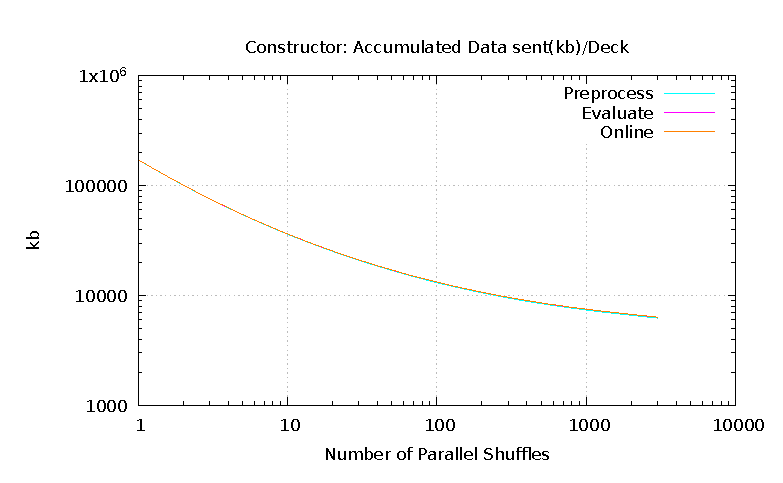
\includegraphics[width=\textwidth]{figurs/const_kb_log_xy.eps}
        }
        \caption{}
        \label{fig:const_kb_plot}
    \end{subfigure}

    \vspace*{0cm}

    \begin{subfigure}{\textwidth}
        \centering
        \scalebox{.7}{
        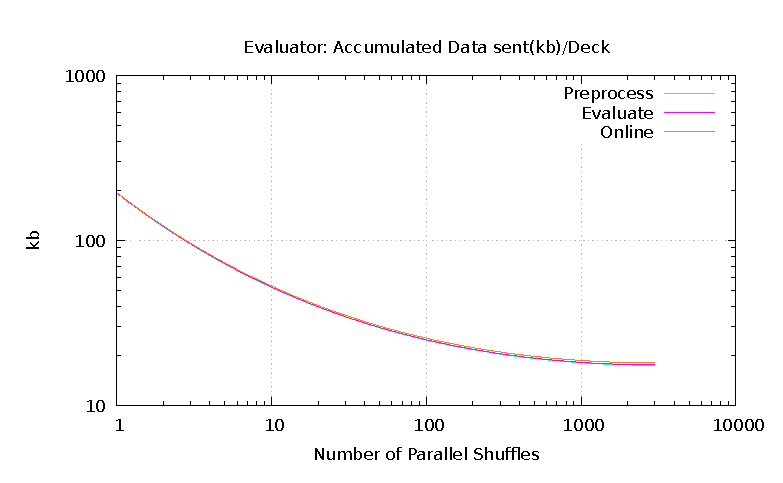
\includegraphics[width=\textwidth]{figurs/eval_kb_log_xy.eps}
        }
        \caption{}
        \label{fig:eval_kb_plot}
    \end{subfigure}

    \vspace*{0cm}

    \begin{subfigure}{\textwidth}
        \centering
        \scalebox{.7}{
        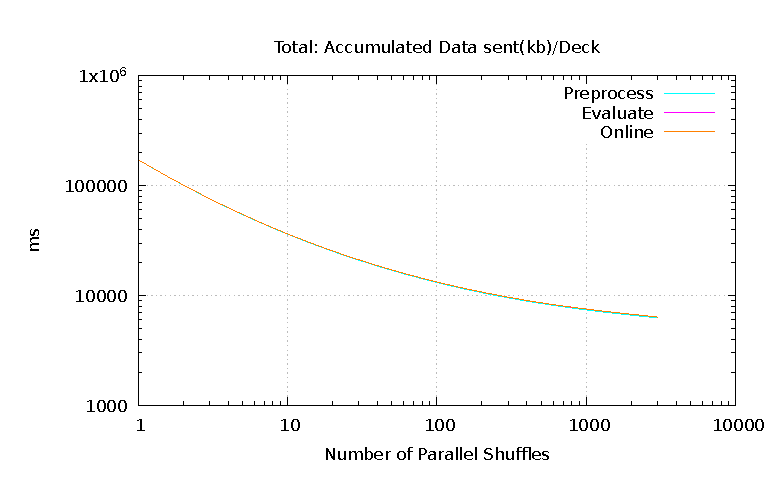
\includegraphics[width=\textwidth]{figurs/total_kb_log_xy.eps}
        }
        \caption{}
        \label{fig:total_kb_plot}
    \end{subfigure}

    \caption{Data sent: Comparison of $Constructor$ and $Evaluator$ in $kb$'s sent to the other party. (a) $Constructor$: Accumulated data sent per deck shuffled on a double logarithmic scale. (b) $Evaluator$: Accumulated data sent per deck shuffled on a double logarithmic scale. (c) $Total$: Accumulated data sent per deck shuffled on a double logarithmic scale.}
    \label{fig:mesurement_kb}
\end{figure}

The first we will look at is the amount of data send in $kb$ per shuffled deck. We see the accumulated data sent per deck shuffled. The data is represented on a double logarithmic scale, to be easier to see the development. It is easy to see that as more simultaneous shuffles are done the less data is sent per deck shuffled. This implies that the most data sent is the overhead, of setting up the protocol. As we see it is hard to distinguish the different lines on the plot. This implies as expected that the $Preprocess$ phase is the one where the most data is communicated between the parties. Relative to this nearly no data is sent in the $Evaluate$ and $Online$ phase. Remembering that it is only the input to the functionality that is sent in the $Evaluate$ phase, which is $830$ bits for each shuffle. In the $Online$ phase we call \verb|DecodeKeys| three times and therefore is it only these keys that are sent. For the $Preprocess$ phase the information of the garbling, soldering and authentication is to be sent, which requires more communication.

In figure \ref{fig:eval_kb_plot} we see that the line is flattening out indicating that there are not much more to gain in shuffling more deck on the $Evaluator$ site. If we then look at figure \ref{fig:const_kb_plot} we see a different tendency where the plot is still decreasing, indicating that some gain can still be done on the $Constructor$ site of the protocol. This may indicate that doing more then $3000$ simultaneous shuffles, can bring the amount of data sent per shuffle further down when looking at the total amount of data sent in the protocol, which can be seen in \ref{fig:total_kb_plot}. When consulting the graph of the total amount of data sent by the parties we see that it is still decreasing, indicating that more is still to be gained in terms of the data transmission. Looking at the scale on the $kb$ axis, it is obvious that it is the $Constructor$ that sends the most data and therefore the one that require the most simultaneous shuffles to bring the overhead of using \DUPLO down.

\bigskip

In this experiment we see exactly what we expected as described above. The amount of $kb$ sent would decrease as more shuffles were done because of the overhead of using \DUPLO. Even going beyond the $3000$ shuffles seems to give a decrease in terms of data sent. The gain of going beyond the $3000$ mark is not nearly as significant as the gain of doing the first $100$.

\bigskip

\begin{figure}
    \centering

    \begin{subfigure}{\textwidth}
        \centering
        \scalebox{.7}{
        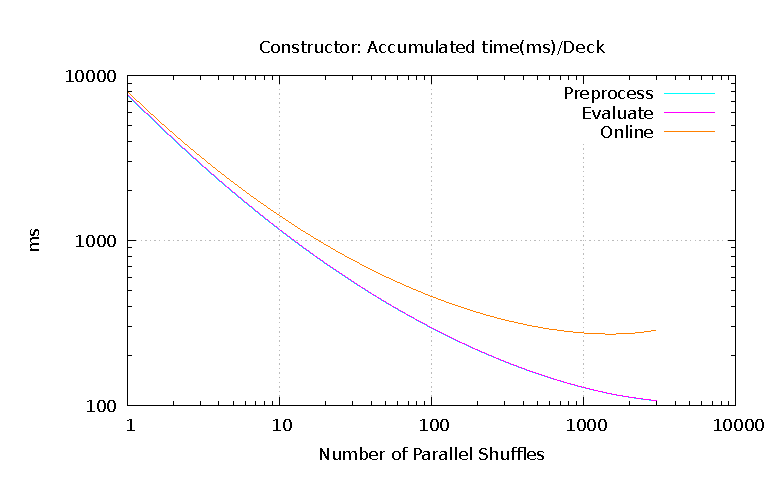
\includegraphics[width=\textwidth]{figurs/const_ms_log_xy.eps}
        }
        \caption{}
        \label{fig:const_ms_plot}
    \end{subfigure}

    \vspace*{0cm}

    \begin{subfigure}{\textwidth}
        \centering
        \scalebox{.7}{
        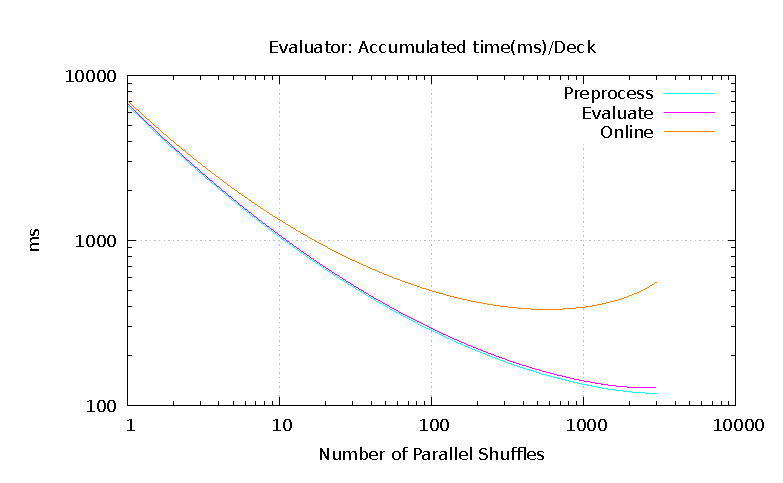
\includegraphics[width=\textwidth]{figurs/eval_ms_log_xy.eps}
        }
        \caption{}
        \label{fig:eval_ms_plot}
    \end{subfigure}

    \vspace*{0cm}

    \begin{subfigure}{\textwidth}
        \centering
        \scalebox{.7}{
        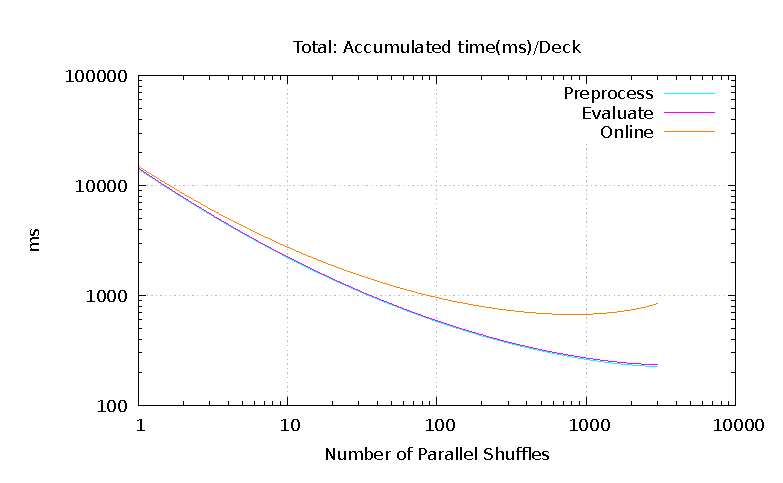
\includegraphics[width=\textwidth]{figurs/total_ms_log_xy.eps}
        }
        \caption{}
        \label{fig:total_ms_plot}
    \end{subfigure}

    \caption{Time: Comparison of $Constructor$ and $Evaluator$ in $ms$'s used. (a) $Constructor$: Accumulated time per deck shuffled on a double logarithmic scale. (b) $Evaluator$: Accumulated time per deck shuffled on a double logarithmic scale. (c) $Total$: Accumulated time per deck shuffled on a double logarithmic scale.}
    \label{fig:mesurement_ms}
\end{figure}

In the next section we will look a the running time used of the framework calls per shuffled deck. This can be seen in figure \ref{fig:mesurement_ms}. The plots are the accumulated running times on a double logarithmic scale. In figure \ref{fig:const_ms_plot} we see the time used in the different phases for the $Constructor$, in \ref{fig:eval_ms_plot} the $Evaluator$ and in \ref{fig:total_ms_plot} summation of these two. On the $Constructor$ side we see that the $Preprocess$ phase accumulates the most of the time. We also see that the time use in this phase is decreasing an approaching $100$ ms per deck shuffled, when shuffling $3000$ decks simultaneous. At the same time we see that the $Evaluate$ phase does not add any significant time. It is a different scenario when looking at the $Online$ phase. Here we see that the space between the $Evaluate$ and $Online$ graphs increases significantly, when approaching $3000$ shuffled deck. This tells us that the $Online$ phase uses more time per shuffled deck, when the amount of shuffles increases. This it not as expected and we will look into that in the next section. For now we can conclude that from the perspective of the $Constructor$, in terms of accumulated running time per shuffled deck, there exists an optimal number of shuffles around $1500$. This optimum will probably variate if tested on other hardware, as the hardware used here are at it limits when doing $3000$ shuffles.
If we the look at the $Evaluator$ in figure \ref{fig:eval_ms_plot} we see the same tendency as for the $Constructor$. The $Preprocess$ is the one consuming the most of the time and here approaching $150$ms per shuffled deck. For the $Evaluate$ phase we see a small increase in time used per shuffle when passing the $1000$ mark. This may be because of the increase in the size of the input to the algorithm. The total time used on these two phases seems to be slightly decreasing. Indicating these can still gain some from doing more shuffles. When we turn our attention to the $Online$ phase, we once again see an increase in the running time. For the $Evaluator$ the increase is more significant than for the $Constructor$ and the optimum is around $500$ shuffles. This is significantly earlier then for the $Constructor$. When we then combine the running times in figure \ref{fig:total_ms_plot}, we see the same tendencies as for the $Constructor$ and $Evaluator$, but with an optimum around $1500$.

\bigskip

This was not the result we had expected. As we discussed earlier we expected the running times to decrease through the complete graph. In the next section we will look into and try to come up with an explanation of why we this results.

\bigskip

\begin{figure}
    \centering

    \begin{subfigure}{\textwidth}
        \centering
        \scalebox{.7}{
        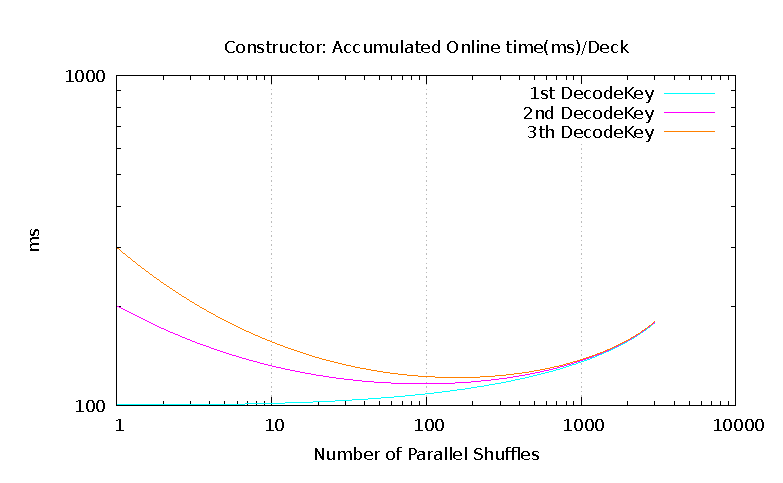
\includegraphics[width=\textwidth]{figurs/const_online_ms_log_xy.eps}
        }
        \caption{}
        \label{fig:const_online_ms_plot}
    \end{subfigure}

    \vspace*{0cm}

    \begin{subfigure}{\textwidth}
        \centering
        \scalebox{.7}{
        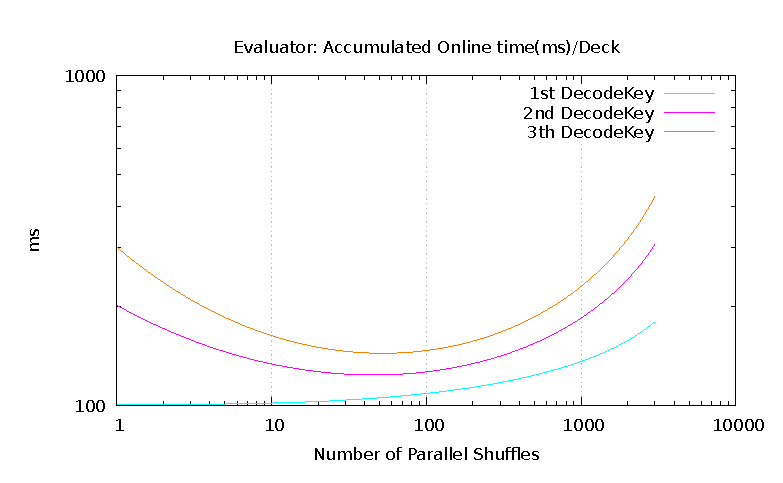
\includegraphics[width=\textwidth]{figurs/eval_online_ms_log_xy.eps}
        }
        \caption{}
        \label{fig:eval_online_ms_plot}
    \end{subfigure}

    \vspace*{0cm}

    \begin{subfigure}{\textwidth}
        \centering
        \scalebox{.7}{
        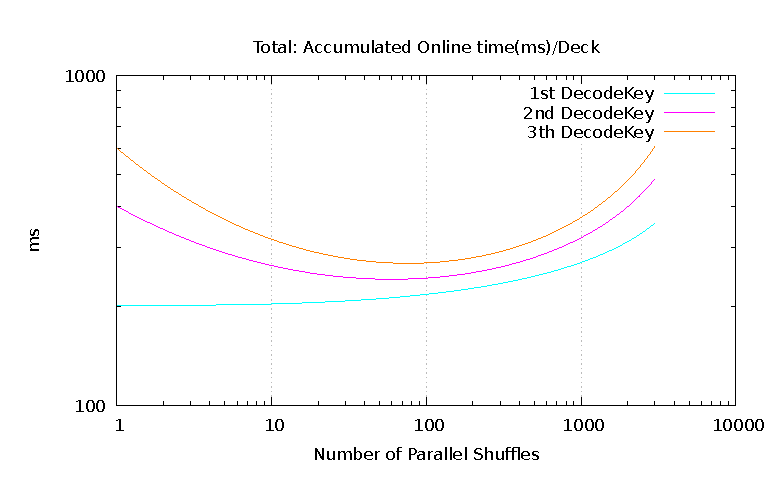
\includegraphics[width=\textwidth]{figurs/total_online_ms_log_xy.eps}
        }
        \caption{}
        \label{fig:total_online_ms_plot}
    \end{subfigure}

    \caption{$Online$ Time: Comparison of $Constructor$ and $Evaluator$ in $ms$'s used in the $Online$ phase. (a) $Constructor$: Accumulated time per deck shuffled on a double logarithmic scale. (b) $Evaluator$: Accumulated time per deck shuffled on a double logarithmic scale. (c) $Total$: Accumulated time per deck shuffled on a double logarithmic scale.}
    \label{fig:mesurement_online_ms}
\end{figure}

We will now take a closer look at the $Online$ phase, to see there are some obvious reasons why we get the results of an increasing $Online$ phase. First off all we start by remember that the $Online$ phase has three calls to the \verb|DecodeKeys| framework function. In figure \ref{fig:mesurement_online_ms} we see the accumulated times used on these \verb|DecodeKeys| calls. The time used by the $Constructor$ can be seen in figure \ref{fig:const_online_ms_plot}. Here we see a increase in the time used on the first \verb|DecodeKeys| call, while the two other calls decreases as expected. This can imply that something happens in the first \verb|DecodeKeys| call, that we did not expect. If we then turn our attention at the $Evaluator$, in figure \ref{fig:eval_online_ms_plot}, we see a graph that looks different from the $Constructor$'s. The main reason is because the most of the work done in the \verb|DecodeKeys| call is done by the $Evaluator$. Here we see an increase in the time used by the first call, while the second and third call firs decreases and then increase again when going towards the $3000$ mark. When consulting figure \ref{fig:total_online_ms_plot} for the combined plot of $Constructor$ and $Evaluator$, we see that the increase in time used by the first \verb|DecodeKeys| call happened before $100$ shuffles, while the increase by the other calls happens after $500$ shuffles. 

The increase in time spent on the \verb|DecodeKeys| calls is probably from the fact that the implementation tries to cache as much as possible. From figure \ref{fig:mesurement_kb} we see that in the $Online$ phase nearly no data is sent. By consulting the data in appendix \ref{app:test-res}, table \ref{table:mesurmet_kb}, we see that approximately $2.5$kb is sent, during the $Online$ phase. Sending this amount of data on a network, with a bandwidth of $1$Gb/s, takes $2.5$ms. As explained earlier the test was done on a network with $50$ms latency. Since we do not know how many rounds of communication the two parties has, we can not conclude any thing from this, beside the fact that this can be seen as a constant. Therefor it must be some implementation specific detail of the framework which is different at the two parties, since we see a fine caching for the $Constructor$ in the second and third call to \verb|DecodeKeys|. The fact that graph looks as it does for the $Constructor$ may indicate that some form of caching is taking place. We cannot say the same about the $Evaluator$, it seems like some caching could take place as the second and third \verb|DecodeKeys| call starts by decrease. What then happens when passing the $100$ shuffle mark is hard to say. The best guess is that the cache may be full and therefore an increase in time is happening, because it has to get the data for a slower memory.

One thing that could support this hypothesis is that it seems like the timings done by each of the \verb|DecodeKeys| calls seems to be more fluctuating when shuffling many decks simultaneous, in a small test I did. This supports the idea that it might be I/O wait that causes the decrease in performance. There simply is a higher risk of some call to wait when shuffling $3000$ decks compared to shuffling $100$. When we then take a look at the time used by each call we see that these task around $100$ms, if a call the has to wait for just $1$ms, we see an increase in time by $1\%$. The problem can also come from the fact that when machines run on high loads their performances go down. When running the $3000$ shuffles test it consumed the most of the memory accessible.

To test this hypothesis of a full cache a test run with the \verb|-d| flag, for the ram only mode, was performed. This did not show any change in the running time other then the uncertainty of the test results. Another approach to cover the reason, could be to take a deeper look at the framework and test the internal structure of the \verb|DecodeKeys| call, to understand what causes this development in the time consumption. This has not been done because of the time limits to this project.

\bigskip

In the next sections I will look into the other things that might affect the protocol. Here it will be the latency on the network and the bandwidth. First off we will start by looking at how the latency affects the \DUPLO protocol, this can be seen in figure \ref{fig:mesurement_delay}. The expectations is to see a decrease in performance when the latency go up, in other words, we expect the running time to go up when the time used on the network goes up. The testing was done with the $1000$ simultaneous shuffle circuit, as this was the constructed circuit closes to the optimum discovered above. The bandwidth was still at the $1$Gb/s mark, to complete the test faster.

\bigskip

\begin{figure}
    \centering

    \begin{subfigure}{\textwidth}
        \centering
        \scalebox{.7}{
        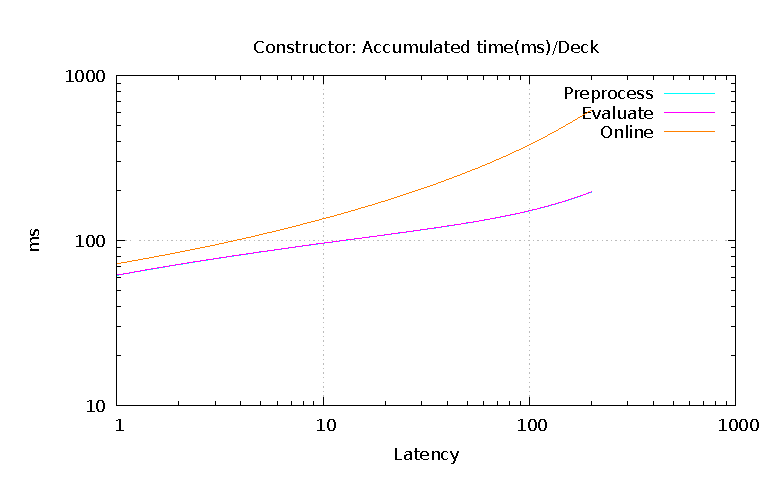
\includegraphics[width=\textwidth]{figurs/const_delay_log_xy.eps}
        }
        \caption{}
        \label{fig:const_delay_plot}
    \end{subfigure}

    \vspace*{0cm}

    \begin{subfigure}{\textwidth}
        \centering
        \scalebox{.7}{
        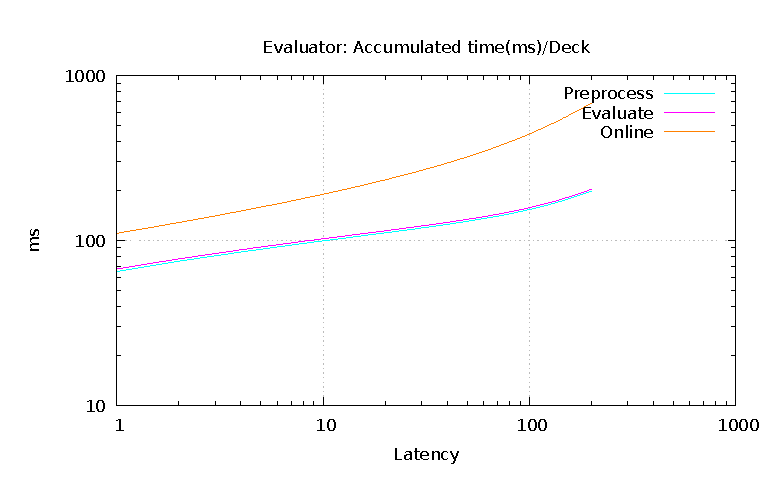
\includegraphics[width=\textwidth]{figurs/eval_delay_log_xy.eps}
        }
        \caption{}
        \label{fig:eval_delay_plot}
    \end{subfigure}

    \vspace*{0cm}

    \begin{subfigure}{\textwidth}
        \centering
        \scalebox{.7}{
        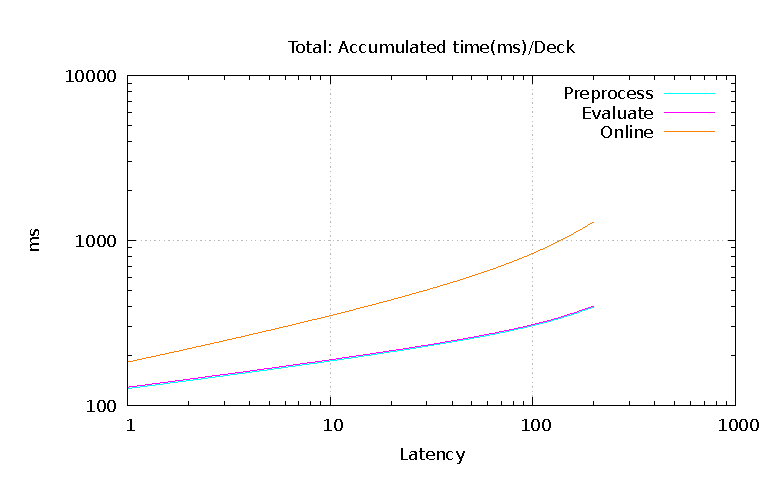
\includegraphics[width=\textwidth]{figurs/total_delay_log_xy.eps}
        }
        \caption{}
        \label{fig:total_delay_plot}
    \end{subfigure}
    \caption{Delay: Comparison of $Constructor$ and $Evaluator$ in $ms$'s used when $1000$ shuffles are done with different latency on the network. (a) $Constructor$: Accumulated time per deck shuffled on a double logarithmic scale. (b) $Evaluator$: Accumulated time per deck shuffled on a double logarithmic scale. (c) $Total$: Accumulated time per deck shuffled on a double logarithmic scale.}
    \label{fig:mesurement_delay}
\end{figure}

In figure \ref{fig:total_delay_plot}, the overall impression is that the protocol handles delay in a constant increasing way. When looking at the $Constructor$ in figure \ref{fig:const_delay_plot} we see that the $Online$ phase is the one effected the most by the network latency, the same is the case for the $Evaluator$ but not as severely. As argued before the $Online$ phase uses a significant amount of time on the network. Therefor an increase in the delay on the network would affect this part of the protocol the most. When comparing these graphs with table \ref{table:ping}, it seems the protocol is performing fine for the latency's found there.

\bigskip

I will now turn the focus towards the benchmarking of the protocol against the bandwidth. To perform this test the $1000$ shuffle circuit was used once again. This time the latency was turned down to $0$ to speed up the process. The expectations of the test is to see a decrease in running time when the bandwidth goes up. It is worth mentioning that no tests are done with bandwidths slower then $50$Mb/s, because the test machine crashed when trying to perform test below this threshold. If consolidating the statistic\footnote{See link in footnote \ref{footnote:bandwith_stats} on page \pageref{footnote:bandwith_stats}.} a bandwidth of $50$ms is within the once used. 

\bigskip

\begin{figure}
    \centering

    \begin{subfigure}{\textwidth}
        \centering
        \scalebox{.7}{
        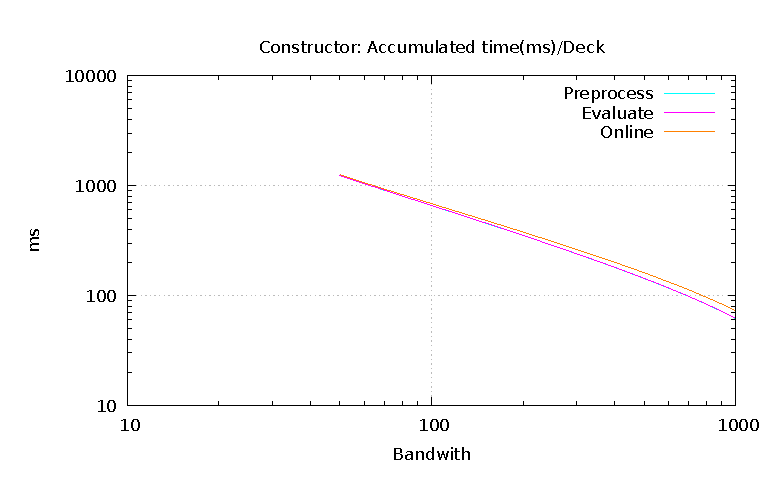
\includegraphics[width=\textwidth]{figurs/const_bandwith_log_xy.eps}
        }
        \caption{}
        \label{fig:const_bandwith_plot}
    \end{subfigure}

    \vspace*{0cm}

    \begin{subfigure}{\textwidth}
        \centering
        \scalebox{.7}{
        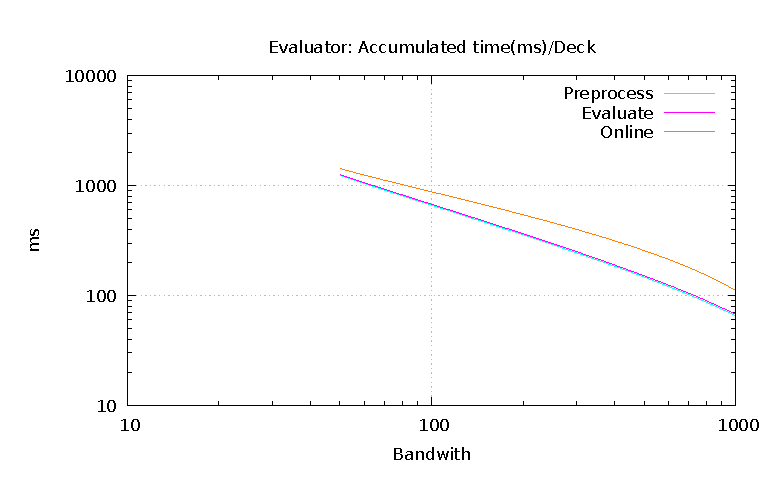
\includegraphics[width=\textwidth]{figurs/eval_bandwith_log_xy.eps}
        }
        \caption{}
        \label{fig:eval_bandwith_plot}
    \end{subfigure}

    \vspace*{0cm}

    \begin{subfigure}{\textwidth}
        \centering
        \scalebox{.7}{
        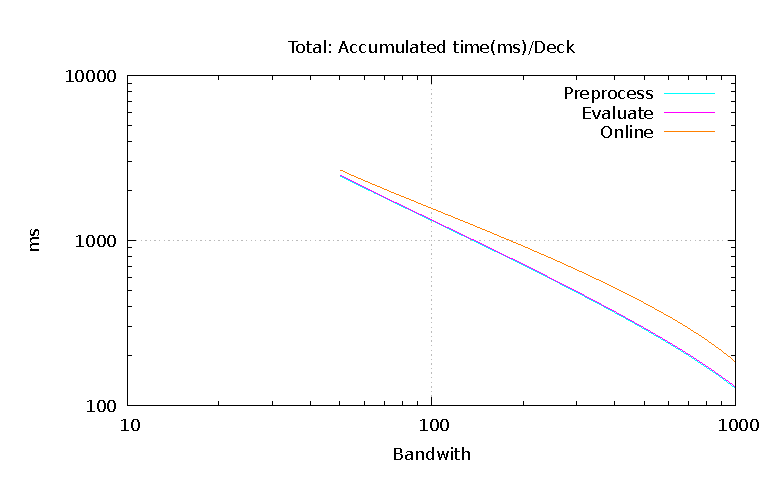
\includegraphics[width=\textwidth]{figurs/total_bandwith_log_xy.eps}
        }
        \caption{}
        \label{fig:total_bandwith_plot}
    \end{subfigure}
    \caption{Bandwidth: Comparison of $Constructor$ and $Evaluator$ in $ms$'s used when $1000$ shuffles are done with different bandwidth on the network. (a) $Constructor$: Accumulated time per deck shuffled on a double logarithmic scale. (b) $Evaluator$: Accumulated time per deck shuffled on a double logarithmic scale. (c) $Total$: Accumulated time per deck shuffled on a double logarithmic scale.}
    \label{fig:mesurement_bandwith}
\end{figure}

The results of the bandwidth test can be found in figure \ref{fig:mesurement_bandwith}. Here we see some fine constant decreasing graphs, both when consulting the graph for the $Constructor$, $Evaluator$ and the total. We see that the $Online$ phase leaves the $Evaluate$ phase a bit to come closer again. This is most probably do to the uncertainty of the testing environment. Overall this follows the expectations we had.

\bigskip

In this section I have tried to cover the tests done an argue for how they were performed. I have discussed the results we have seen and try to argue for why they are a they are. If the results was not as expected I have tried to cover these areas with new results within the time limit of the project. In the next section I will try to hold the results from this section up against what can be expected in of running times of real online poker.

\section{Discussion}
\label{sec:discussion}

In this section the benchmarking done in section \ref{sec:bechmarking} will be compared to what can be expected in the real world. I will discuss both settings of the poker game introduced in section \ref{sec:poker_imp}. This will be done because some of the settings used when testing fits best in one setting and others in the other.

The first setting that will be discussed is the setting implemented, where the $Constructor$ and $Evaluator$ both play the part of server and client. Before comparing this setting to the real world an discussion of the different parameters used will be done. If we start by looking at the latency used in figure \ref{fig:mesurement_ms}. This was done using $50$ms delay, compared to table \ref{table:ping} it seems to be a fair latency between two player in the real world. The bandwidth in this setting was set to $1024$Gb/s, as argued above this is to high when compared to statistics\footnote{Same as in footnote \ref{footnote:bandwith_stats} on page \pageref{footnote:bandwith_stats}}. Correcting the results according to this will imply that more time would be added to the running time. This can be done by combining the results from figure \ref{fig:mesurement_ms} and figure \ref{fig:mesurement_bandwith}. If we use the timing of the$50$Mb/s, then when doing $1000$ shuffles we would have to add around $1$ second to the running time per deck shuffled. This will yield a total running time of around $1.2$ second per deck for the $Constructor$ and $1.5$ for the $Evaluator$. Here it is important to remember that the time used in the $Preprocess$ phase can be done ahead of time. It may also be fair to argue that for two player to play $1000$ hands may be to the high site, as the preparation of the protocol can be done in a cycle, such that the preprocessing is done when they do not play. By reducing the amount of shuffles the running time per deck will go up but the total time may go down. We can then argue that the hardware used is to the extreme end when comparing to ordinary household machines, this may imply that the optimal number of simultaneous shuffles will be reduced and therefore fit better with the discussion about $1000$ shuffles being to many. This may yield an optimum around $500$ shuffles. From the test done it is not possible to conclude on the exact time of such a game but an estimate would be below $1.5$ seconds per shuffle, in total $1000$ seconds which is around $13$ minute. Consolidating the graph the $Preprocess$ phase uses approximately the half of this time, in this case around $7$ minutes. By doing this preprocess the players are then able to play $500$ games of poker, with a running time of $6$ minutes in total. This yields a running time of just below $75$ms per game. Here we remember that the tests are done automatically without any change of cards, but when two players are playing against each other the decision of choosing cards would be significantly longer then this. Therefore we may argue that performance of the poker implementation is good if the time for the preprocessing is not to high. In this setting we argue that on a consumer computer it will take around $7$ minutes to preprocess $500$ decks. Two players of this type, must be assumed to leave their computer for more then $7$ minutes a day, and therefore may the protocol actually do well in this setting.

In the other setting where the $Constructor$ and $Evaluator$ plays the role of servers, but not clients them self, we may argue that we will see some other results. Once again the latency used during the test seems to be fair. The bandwidth used during the test may also be fair in this setting since servers prioritize a higher bandwidth to handle a big load. In this setting we may argue that $1000$ shuffles is to few.  The $1000$ shuffles takes around $1.2$ seconds for the $Constructor$ and $1.5$ for the $Evaluator$ per deck shuffled as argued above. Yielding $20$ minutes for the $Constructor$ and $25$ minutes for the $Evaluator$. We may argue that a poker provider use more then $1000$ decks in $25$ minutes, and the fact that no games can be played while the servers is in the $Preprocess$ phase. This problem can be handled by having two sets of servers one preprocessing enough games to last the time it takes for the other set of servers to do their preprocessing. Then we may argue that servers of poker providers have more computation power then the hardware used during the test and therefor can handle more simultaneous shuffles and therefor may be able to produce a greater amount in the same time. In this setting it is hard to argue whether the protocol can handle the task or not. In this setting we do not have the ability to do the preprocess when no game is ongoing, but the phase where the clients are dealt the cards are still acceptable, as it will be hidden in the choice of cards to be changed as argued above.

\bigskip

All in all, the we seem to be able to draw the conclusion that the poker game implemented using \DUPLO in this project can actually handle real world scenarios. The biggest concern is to find the time to do the preprocessing, but is a setting used where the time to the preprocessing can be found, then is the running time in the other phases acceptable.

In the next chapter, I will do a summary of the project and reflect the conclusion done in this section. I will introduce some future work that could be done to see how things stack up in different scenarios and why I got the results I did.

%%%%%%%%%%%%%%%%%%%%%%%%%%%%%%%%%%%%%%%%%%%%%%%%%%%%%%%%%%%%%%%%%%%%%%%

\chapter{Conclusion}
\label{ch:conclution}

In this chapter I will try to do a summary of the project and conclude on the results found in chapter \ref{ch:implementation}.

In this project I have studied the application of using the \DUPLO framework and protocol in the setting of a poker game. This was done to see how using a two party computation protocol will affect the overall running time and see if the protocols are mature enough to be used in real world situation. To do this the \DUPLO protocol was chosen, which is a secure two party computation protocol, using garbled circuits. This was chosen, because it has the possibility to do unique single wire opening, the existence of a circuit compiler and the fact that is developed at Aarhus University. Because of the security of \DUPLO we are guaranteed to be able to provide privacy, correctness and independence of input. Privacy is the ability of the protocol to ensure that nothing more than the output is leaned. Correctness it the ability of the protocol to guarantee that the right output is provided to the parties. Independence of input is the ability of the protocol to guarantee that the input of one of the parties can not depend on the input of the other. Because these properties is given from the protocol we can start looking at the decision that should be made before the implementation could begin.

First a decision was made on the setting of how the protocol should be used. This could either be a setting where the two parties of the protocol acted as both server and client, or one where they only acted as server. The setting where the both acted as server and client, was the one chosen mainly because of its simplicity and the time limit of the project. The other setting is proposed as a future work below, for others to look into.

A decision of which type of poker game to implement also had to be done. Here the five card draw variant was chosen. This was done mainly because it is the variant of poker used the most games when only two players participate. When only two parties participate it allowed for some optimizations of the shuffle algorithm, such a smaller circuit could be produced for evaluation in the protocol.

To be able to use the \DUPLO protocol in the poker implementation we needed to generate the functionality that should be used. In this case it was the shuffling of the cards, that should be handled by \DUPLO. We looked into different algorithms to compare their circuit size, to be able to choose the one giving the fast's run time of the protocol. Because the complexity of circuits is high when the complexity of the functionality implemented gets higher then simple a compiler was used to generate the circuits. This allowed for a higher level of abstraction. The \FY and \CS algorithm was then implemented, both in a non-optimized and optimized version. This was done to see the affect of only shuffling the cards necessary when only two players participated in the poker game. Based on the comparison of the shuffle algorithms the optimized version of \CS was the one chosen.

The implementation of the game could then start. The \DUPLO protocol stated the order of the framework calls. The main purpose of the implementation was to generate the inputs to the protocol at the right time. Because of the way the \DUPLO framework had splitted the functions, three different phases was made. The first phase was based on the functionality of the circuits where this was garbled, such that it could be securely evaluated. This is denoted the preprocessing phase, as it can be done only based on the circuit generated. The second phase was the evaluation phase where the input to the functionality was given and the garbled circuit evaluated. The last phase was the online phase, this was the phase where per player would be shown their hand, chose which cards to change and see the opponents cards. No betting or declaration of a winner was implemented because of the time limits to the project. The betting functionality is proposed as future work as it could be interesting to see if this could be done using another secure protocol. Now that the implementation was in place the testing could begin.

During the benchmarking different parameters was tested to see how the \DUPLO protocol handled these settings. Because the \DUPLO protocol should perform better when working with big circuits, different variants of the \CS shuffle was generated where different amount of shuffled decks was generated. This was done to see how big the benefit was of doing many simultaneous shuffles. The expected result was that it would perform better and better, but this was not the case. We saw that there existed an optimum for the protocol. This is probably because of the internal optimizations of the protocol where it tries to cache as much as possible, and when the limit of the cache is exceeded the performance decreases. The optimal number of shuffles was then used to test how the protocol reacted to different amounts of latency on the network. The expectation was that it would have a linear slowdown in performance when the latency on the network went up. This was also the results we got when performing the benchmark. The optimal circuit was then also used to test how the bandwidth affected the protocol. Here the expectations was that we would see a linear increase in performance when the bandwidth went up. One again it performed as expected. When the benchmarks was done the running times from these was then compared to what could be expected of a real world poker game.

When looking at the numbers for the the setting studied in the project we may conclude that the poker implementation using the \DUPLO protocol can achieve running times that are good. When discussing the benchmarks the numbers of playing $500$ hands of poker between to players yields $7$ minutes used on preprocessing and evaluation of the circuit and less then $75$ms for each game played. The $75$ms is negligible when comparing to the time used by the player to decide which cards to keep and which to change. Furthermore the time is determined by the network latency which is $50$ms in this estimate of time. Therefor all in all the performance achieved is good, but the most online poker games are not played in this setting. Therefor and argument was done to try to compare it to that setting. Here we a down period for preprocessing the shuffles cannot be tolerated. This can be handled by letting to systems run in parallel where one preprocess shuffles while the other deals cards. As argued this setup is only feasible if the time it takes for players to play the amount of shuffles produced during the preprocess phase exceeds the time it takes to preprocess them. This haven been studied but as argued in the discussion of the benchmarking the online timings are feasible enough for the protocol to work in this setting, the questing is if the latency, bandwidth, and hardware of online poker providers allow them to preprocess shuffles fast enough. This can not be concluded before tested in such a setting, but the performance of secure two party computation are closing the gab to be feasible in real world applications.

\bigskip

In the next section I will come up with some proposals to further work that could be done based on this project and the \DUPLO protocol.

\section{Proposed future work}
Here I will propose some interesting aspects i have touched during the project but have not had the time to look into. Each of the proposals should be possible to cover in the time of a project. Some of them might not be for a thesis, but could be used as a preproject to get into the \DUPLO protocol and the working mechanisms of a $MPC$. I will give each project a short paragraph on why this could be interesting and how this could be done.

\paragraph{DecodeKeys running time coverage:}
In this project the development of the running times of the \verb|DecodeKeys| call could be studied. It could be interesting to get a deeper understanding of why we see the development in the graphs in figure \ref{fig:mesurement_online_ms}, as we do. This could be done by going in to the framework an time the different calls made inside of the \verb|DecodeKeys| function. It could be interesting to see if the hypothesis of the full cache is the reason or something else. It could also be interesting to see the differences at the two parties, why do the timings differentiate in such a way they do.

\paragraph{\DUPLO in a server setting:}
It could be interesting in this project to study how the \DUPLO protocol would perform in the setting where the $Constructor$ and $Evaluator$ acts and servers and not clients at the same time. How would the authenticity and correctness of the inputs be guaranteed. Would the addition of these properties add an extra overhead to the \DUPLO protocol making it perform significantly worse, or will it handle it well. 

\paragraph{Five card draw vs. Texas Hold'em:}
This project could be interesting to see especially in the server setting where more then two player could participate. Overall it could be interesting to see how much the difference in the optimization of the circuit will affect the running times. In a two party setting only $9$ cards is used in Texas Hold'em compared to the $20$ in five card draw.

\paragraph{Addition of betting:}
Betting is a big part of online poker, therefore could it be interesting to add this to the implementation. This could be done by using smart contract in block chain. by doing it this way the money will only be transferred if a condition is satisfied. Some but not all cryptocurrency protocols allows for these contracts, but I think it should be possible to do.


%%%%%%%%%%%%%%%%%%%%%%%%%%%%%%%%%%%%%%%%%%%%%%%%%%%%%%%%%%%%%%%%%%%%%%%

\begin{appendices}
\chapter{Code base}
In this appendix references will presented to the different Code base used during the thesis. An URL to the repositories on GitHub will be presented together with a short description of where the most interesting parts for this project can be found.

\section{Hardware}
\label{app:hardware}
For compilations of the circuits with the $Frigate$ compiler the following setup has been used:

\begin{center}
\begin{verbatim}
OS:        Ubuntu 16.10/17.04
Processor: Intel i5-4210U CPU @ 1.70GHz
Cores:     2
Threads:   4
RAM:       12 GB
\end{verbatim}
\end{center}

I did not encounter any problems or slow compilations of circuits using this setup.

\bigskip
For the testing of the poker game that setup was not sufficient as it could not handle more than 500 simultaneous shuffles. Therefore another setup up was used:

\begin{center}
\begin{verbatim}
OS:        Ubuntu 16.04 LTS
Processor: Intel i7-3770K CPU @ 3.50GHz
Cores:     4
Threads:   8
RAMS:      32 GB
\end{verbatim}
\end{center}

This setup allowed for testing up to 3000 simultaneous shuffles, which is the highest done in the testing phase. When going up to 4000 this setup ran out of memory on the $Evaluator$ site of the execution.


\section{DUPLO}
\label{app:duplo}
The \DUPLO repository at GitHub can be found here \footnote{\url{https://github.com/AarhusCrypto/DUPLO}}.

The documentation on the site is clear and illustrates clearly how it is compiled such it can be tested. No documentation is presented for how interacting with the framework can be done for new implementations. The most interesting part for the sake of this project is located in the \verb|src| folder. Here the \verb|CMakeLists.txt| file is located which specifies how the project is compiled, this is overwritten when compiling the poker implementation. The folder \verb|src/duplo-mains| is where the actual implementations of the $Constructor$ and $Evaluator$ can be found. Here the implementations of the poker $Constructor$ and $Evaluator$ will be placed.

\bigskip

For a easy setup of duplo a docker instance is created and can be found here \footnote{\url{https://hub.docker.com/r/cbobach/duplo/}}. This can be started in docker version \verb|17.05.0-ce| with the command;

\begin{center}
\begin{verbatim}
docker run -it --network:host cbobach/duplo
\end{verbatim}
\end{center}

The \verb|--network:host| flag is not secure but is the fart easy way to let the container running the $Constructor$ expose the port on which the container running the $Evaluator$ needs to connect. When running two instances of these docker containers the $Constructor$ and $Evaluator$ is run using one for these commands for the default setting:

\begin{center}
\begin{verbatim}
./build/release/DuploConstructor 
./build/release/DuploEvaluator
\end{verbatim}
\end{center}


\section{Frigate}
\label{app:frigate}
The $Frigate$ repository on GitHub is a sub-repository to \DUPLO and can be found here \footnote{\url{https://github.com/AarhusCrypto/DUPLO/tree/master/frigate}}.

The documentation of how $Frigate$ is installed with the special versions of some of the libraries used is specified in the documentation of \DUPLO, the link can be found in appendix \ref{app:duplo}. It is also here the documentation of how to compile \DUPLO circuit formats are done.

To find the documentation of the \verb|.wir| file format a look should be taken at the link above. Here the specifications are of how wire access is done for example. It is here all functionalities that are implemented in the language is listed and how they are used. This documentation is narrow at some places. It does for example not specify that the modulo operator \verb|%| does only work on powers of $2$.

\bigskip

Using the docker image from docker \footnote{\url{https://hub.docker.com/r/cbobach/duplo/}} and running the following command, in docker version \verb|17.05.0-ce|;

\begin{center}
\begin{verbatim}
docker run -it -v host/dir:container/dir cbobach/duplo
\end{verbatim}
\end{center}

will start a container where it is possible to compiler a \verb|.wir| file using the container. For it to work the \verb|.wir| files has to be located in the \verb|host/dir| then the following command can be run to compile the functionality:

\begin{center}
\begin{verbatim}
./build/release/Frigate container/dir/functionality.wir -dp
\end{verbatim}
\end{center}

The \verb|-db| flag ensures that the \DUPLO file format is generated. The \DUPLO generate file will have the extension \verb|.wir.GC_duplo| this can then be fed to the \DUPLO framework using

\begin{center}
\begin{verbatim}
./build/release/DuploConstructor -f container/dir/functionality.wir.GC_duplo
./build/release/DuploEvaluator -f container/dir/functionality.wir.GC_duplo
\end{verbatim}
\end{center}

Then the new functionality will be run in the default \DUPLO environment.

\section{Poker}
\label{app:poker}
In this section the GitHub repositories to the different phases will be linked. A short description to where the interesting parts are will be presented.

\subsection{Circuit implementation}
\label{app:circuit-impl}
The different circuit \verb|.wir| files can be found in the GitHub repository here \footnote{\url{https://github.com/cbobach/speciale_circuit}}.

Here the implementations of the shuffle algorithms are present as \verb|fisher_yates_shuffle.wir| and \verb|conditional_swap_shuffle*.wir|. Multiple versions of the \verb|conditiona_swap_shuffle*.wir| file are present with different values for \verb|*|. This is to allow for multiple sequential hands to be played, these files are then used when testing the \DUPLO framework to show its capabilities.

Only one version of \verb|fisher_yates_shuffle.wir| is located in the repository since this is a slower algorithm in this setting as discussed in section \ref{sec:comp}.

The files \verb|init_deck.wir|, \verb|xor_seed.wir| and \verb|correcred_seed.wir| are all modules that are called by the shuffle algorithms. The \verb|init_deck.wir| file is used by both algorithms and hard wires the card values to their respective wires. The \verb|corrected_seed.wir| file is used by the \FY algorithm to ensure that the seed fed to the shuffle algorithm is in the correct intervals as explained in section \ref{sec:fisher-yates}. The \verb|xor_seed.wir| file is used by the \CS algorithm to generate the seed used by the shuffle.

\bigskip

It is also here that the parser used to debug the $Frigate$ compiler is located and is found as \verb|parse.py|. The other python script found in \verb|count-gate-types.py| is the one used to compare the amount of gates types for the compiled circuits.


\subsection{DUPLO implementation}
\label{app:duplo-impl}
The poker repository for the implementation using the duplo framework can be found here \footnote{\url{https://github.com/cbobach/speciale_implementation}}.

Here the \verb|CMakeLists.txt| file is the one used to overwrite the original file found in the \DUPLO framework to allow for compilation of the poker $Constructor$ and $Evaluator$. In the folder \verb|duplo-mains| the implementations of these are located as \verb|poker-const-main.cpp| for the $Constructor$ and \verb|poker-eval-main.cpp| for the $Evaluator$. In this folder their shared functionality is found in the \verb|poker-mains.h|.

\bigskip

Back in the main dir of the repository the docker files are found for generating the docker instance of \DUPLO used in appendix \ref{app:duplo} and \ref{app:frigate}. This is the \verb|Dockerfile.DUPLO| where as the \verb|Dockerfile| is the one used for running the poker implementation. The \verb|entry-point.sh| files is used to start the docker containers correct such that they can run in the background. The docker image can be found here \footnote{\url{https://hub.docker.com/r/cbobach/duplo-poker/}}. The containers can be started using the following commands in docker:

\begin{center}
\begin{verbatim}
docker run -d -p 2800:2800 cbobach/duplo-poker --profile const -i 0
docker run -d -network:host cbobach/duplo-poker --profile eval -i 0
\end{verbatim}
\end{center}

The \verb|-d| flag tells docker that the containers should run detached. The \verb|-p| flags tells docker to connect the host port $2800$ to the containers internal port 2800. \verb|--network:host| is the easy way to let the container have access to the hosts network ports. These commands will play one hand of poker in the background, if more are required the \verb|-f| flag can be used to specify which circuits should be used. To get the the right timings the \verb|-n| flag is required together with the \verb|-f| flag. This flag needs to reflect the number of simultaneous shuffles in the circuit.

Using the \verb|-it| flag in docker instead of the \verb|-d| flag allow for interactive rounds of poker if the \verb|-i| flag is set to $1$ instead of $0$.


\subsection{Test results}
\label{app:test-res}
In this section a link to the repository on GitHub with all the generated statistics. Here all generated graphs and timings can be found. The repository can be found here \footnote{\url{https://github.com/cbobach/speciale_thesis/tree/master/figurs}}

\bigskip

In the tables here the actual data used to generate the figure \ref{fig:mesurement_kb} and \ref{fig:mesurement_ms} in section \ref{sec:bechmarking} can be found.

\begin{table}
\centering

    \begin{subtable}{\textwidth}
    \label{table:const_kb}
    \centering
    \scalebox{1}{
    \begin{tabular}{l || r r r r r}
               & \multicolumn{5}{c}{Number of Parallel Shuffles} \\
    Phase      &         1 &       10 &     100 &    1000 & 3000 \\
    \hline
    Preprocess & 172140.31 & 26817.94 & 9380.99 & 7380.56 & 6219.38  \\
    Evaluate   &    122.84 &   122.84 &  122.84 &  122.84 &  122.84  \\
    Online     &      5.94 &     2.38 &    2.02 &    1.99 &    1.99  \\
    \hline
    Total      & 172269.09 & 26943.16 & 9505.85 & 7505.42 & 6344.21
    \end{tabular}
    }
    \caption{$Constructor$}
    \end{subtable}%
    
    \vspace*{.5cm}
    
    \begin{subtable}{\textwidth}
    \label{table:eval_kb}
    \centering
    \scalebox{1}{
    \begin{tabular}{l || r r r r r}
               & \multicolumn{5}{c}{Number of Parallel Shuffles} \\
    Phase      &      1 &    10 &   100 &  1000 & 3000 \\
    \hline
    Preprocess & 193.75 & 36.59 & 19.15 & 17.57 & 17.50 \\
    Evaluate   &   0.11 &  0.10 &  0.10 &  0.10 &  0.10 \\
    Online     &   1.44 &  0.58 &  0.49 &  0.48 &  0.48 \\
    \hline
    Total      & 195.30 & 37.27 & 19.74 & 18.15 & 18.08
    \end{tabular}
    }
    \caption{$Evaluator$}
    \end{subtable}%

    \vspace*{.5cm}
    
    \begin{subtable}{\textwidth}
    \label{table:eval_kb}
    \centering
    \scalebox{1}{
    \begin{tabular}{l || r r r r r}
               & \multicolumn{5}{c}{Number of Parallel Shuffles} \\
    Phase      &         1 &       10 &     100 &    1000 & 3000 \\
    \hline
    Preprocess & 172334.06 & 26854.53 & 9400.14 & 7398.13 & 6236.88 \\
    Evaluate   &    122.95 &   122.94 &  122.94 &  122.94 &  122.94 \\
    Online     &      7.38 &     2.96 &    2.51 &    2.47 &    2.47 \\
    \hline
    Total      & 172464.39 & 26980.43 & 9525.59 & 7523.57 & 6362.29 
    \end{tabular}
    }
    \caption{$Total$}
    \end{subtable}%

    \caption{Data sent: Comparison of $Constructor$ and $Evaluator$ in $kb$'s sent to the other party. (a) $Constructor$: $kb$'s data sent in different phases. (b) $Evaluator$: $kb$'s data sent in different phases.}
    \label{table:mesurmet_kb}
\end{table}

\begin{table}
    \centering

    \begin{subtable}{\textwidth}
    \centering
    \scalebox{1}{
    \begin{tabular}{l ||r r r r r}
          & \multicolumn{5}{c}{Number of Parallel Shuffles} \\
    Phase      &       1 &      10 &    100 &   1000 & 3000    \\
    \hline
    Preprocess & 8202.12 &  918.74 & 193.32 & 116.73 & 106.89 \\
    Evaluate   &  100.82 &   10.22 &   1.18 &   0.30 &   0.30 \\
    Online     &  301.09 &  120.84 & 103.38 & 116.60 & 179.35 \\
    \hline
    Total      & 8604.03 & 1049.80 & 297.88 & 233.63 & 286.54 
    \end{tabular}
    }
    \caption{$Constructor$}
    \label{table:const_ms}
    \end{subtable}%

    \vspace*{.5cm}

    \begin{subtable}{\textwidth}
    \centering
    \scalebox{1}{
    \begin{tabular}{l || r r r r r}
          & \multicolumn{5}{c}{Number of Parallel Shuffles} \\
    Phase      &       1 &     10 &    100 &   1000 & 3000    \\
    \hline
    Preprocess & 6619.65 & 823.37 & 187.27 & 119.74 & 118.28\\    
    Evaluate   &  129.49 &  17.91 &   5.43 &   5.44 &   9.58 \\
    Online     &  301.76 & 121.09 & 116.34 & 159.80 & 430.11\\
    \hline
    Total      & 7050.90 & 962.37 & 309.04 & 284.98 & 557.97
    \end{tabular}
    }
    \caption{$Evaluator$}
    \label{table:eval_ms}
    \end{subtable}%

    \vspace*{.5cm}

    \begin{subtable}{\textwidth}
    \centering
    \scalebox{1}{
    \begin{tabular}{l || r r r r r}
          & \multicolumn{5}{c}{Number of Parallel Shuffles} \\
    Phase      &        1 &      10 &    100 &   1000 & 3000    \\
    \hline
    Preprocess & 14821.77 & 1742.11 & 380.59 & 236.47 & 225.17 \\    
    Evaluate   &   230.31 &   28.13 &   6.61 &   5.74 &   9.88 \\
    Online     &   602.85 &  241.93 & 219.72 & 276.40 & 609.46 \\
    \hline
    Total      & 15654.93 & 2012.17 & 606.92 & 518.61 & 844.51 
    \end{tabular}
    }
    \caption{Total}
    \label{table:eval_ms}
    \end{subtable}%

    \caption{Comparison of $Constructor$ and $Evaluator$ in terms of time consumption in $ms$ during framework calls. (a) $Constructor$: Time consumption in different phases. (b) $Evaluator$: Time consumption in different phases. (c) $Total$: Time consumption in different phases.}
    \label{table:mesurement_ms}
\end{table}


\todo{Add log files to GitHub}

\todo{describe test bash script}



\end{appendices}

%%%%%%%%%%%%%%%%%%%%%%%%%%%%%%%%%%%%%%%%%%%%%%%%%%%%%%%%%%%%%%%%%%%%%%%

\addcontentsline{toc}{chapter}{Bibliography}
\bibliography{references}{}
\bibliographystyle{plain} 

\end{document}